% ---------------------------------------------------------------------------
% The LuPNT Manual -- LaTeX edition.
%
% Build (no system LaTeX required):
%   cd latex_docs && ./build.sh
%
% This document covers LuPNT's design and mathematical specifications: full
% derivations, unit and time-scale contracts, and the implementing C++/Python
% code inline. See README.md for the layout and for the conventions every
% chapter follows.
% ---------------------------------------------------------------------------

% `book` (not `report`) for \frontmatter / \mainmatter / \backmatter.
\documentclass[11pt,twoside,openright]{book}

% ---------------------------------------------------------------------------
% preamble.tex -- shared packages, styles and macros for the LuPNT manual.
%
% Every chapter under chapters/ is written against the contract defined here:
% the listing styles, the \code/\file/\cpp/\py macros, and the label prefixes
% (chap:, sec:, eq:, tab:, fig:).  Chapters must not load packages of their
% own -- add them here so that a chapter stays compilable in isolation via
% \includeonly.
% ---------------------------------------------------------------------------

\usepackage[T1]{fontenc}
\usepackage[utf8]{inputenc}
\usepackage{lmodern}
\usepackage[margin=1in]{geometry}

% --- mathematics ------------------------------------------------------------
\usepackage{amsmath}
\usepackage{amssymb}
\usepackage{bm}
\usepackage{siunitx}
% \year and \day are TeX count registers, so these units need their own
% control sequences rather than the siunitx defaults.
% siunitx's default \micro resolves to \textmu, which under T1 + Latin Modern
% renders as a t-cedilla ("0.3 tps") rather than a mu. Every microsecond,
% micrometre and microradian in the manual goes through this, so redeclare the
% prefix to use the math mu. Verified by rendering, not by text extraction:
% pdftotext maps the broken glyph misleadingly either way.
\DeclareSIPrefix{\micro}{\ensuremath{\mu}}{-6}

\DeclareSIUnit{\yr}{yr}
\DeclareSIUnit{\dayunit}{d}
\DeclareSIUnit{\bit}{bit}
\DeclareSIUnit{\dB}{dB}
\DeclareSIUnit{\dBHz}{dB\text{-}Hz}
\DeclareSIUnit{\dBW}{dBW}
\DeclareSIUnit{\dBi}{dBi}
\DeclareSIUnit{\TECU}{TECU}
\DeclareSIUnit{\au}{au}

% --- tables, figures, floats ------------------------------------------------
\usepackage{booktabs}
\usepackage{longtable}
\usepackage{array}
\usepackage{multirow}
\usepackage{tabularx}
\usepackage{graphicx}
\usepackage{float}

% --- where figures come from ------------------------------------------------
% latex_docs holds text only. Binary artefacts live in one of two places:
%
%   ../assets/               repository-level brand assets, already in git
%   $LUPNT_DATA_PATH/docs/   generated/large artefacts, fetched not committed
%
% build.sh resolves LUPNT_DATA_PATH and writes figpath.tex (gitignored) with
% the absolute path; the \providecommand below is the fallback for a plain
% `pdflatex lupnt` run from this directory.
\IfFileExists{figpath.tex}{\input{figpath}}{}
\providecommand{\datafigdir}{../data/LuPNT_data/docs/}
\graphicspath{{\datafigdir}{../assets/}{../docs/_static/}}

% \datafig[<includegraphics opts>]{<file>} -- include a figure from
% \datafigdir, degrading to a visible placeholder when the data directory has
% not been fetched. A missing artefact must not break the build: the manual has
% to compile from a bare clone.
\newcommand{\datafig}[2][width=\textwidth]{%
  \IfFileExists{\datafigdir #2}{%
    \includegraphics[#1]{#2}%
  }{%
    % \detokenize, not a bare \texttt{#2}: the filename was tokenized at the
    % call site, so its underscores carry catcode 8 and would be read as
    % subscripts. \detokenize re-emits them as printable catcode-12 characters.
    \fbox{\parbox{0.92\textwidth}{\centering\small\vspace{6pt}
      \textbf{Figure not available:} \texttt{\detokenize{#2}}\\[3pt]
      It lives in \texttt{\$LUPNT\_DATA\_PATH/docs/}, which this build could not
      find. See the figure notes in \texttt{latex\_docs/README.md} for how to
      regenerate it.\vspace{6pt}}}%
  }%
}
\usepackage[labelfont=bf,font=small]{caption}
\usepackage{enumitem}
\usepackage{microtype}

% Ragged-right X column: long identifiers in the spec tables must not be
% stretched into rivers.
\newcolumntype{L}{>{\raggedright\arraybackslash}X}

% Weighted ragged-right X column, used directly in a spec as `W{2}`: it takes
% twice the share of a plain `L`. The weights across one tabularx must sum to
% the number of X/L columns -- two columns can be W{1.4} W{0.6}, three can be
% W{1.5} W{1} W{0.5}, and so on. Reach for this instead of a fixed `l`/`r`/`c`
% column whenever a cell holds a phrase rather than a single token: a non-X
% column claims its content's natural width first, so one long cell there
% starves the real X columns until they wrap a word at a time.
\newcolumntype{W}[1]{>{\hsize=#1\hsize\raggedright\arraybackslash}X}
% Right-aligned weighted X, for a numeric comparison column that should still
% be able to wrap a trailing note.
\newcolumntype{Y}[1]{>{\hsize=#1\hsize\raggedleft\arraybackslash}X}

% A fixed-width ragged-right column, used as `P{2.1cm}`: for a token column
% (identifier, path) that is narrow on average but has an entry or two long
% enough that a bare `l` would widen the whole table.
\newcolumntype{P}[1]{>{\raggedright\arraybackslash}p{#1}}

% --- diagrams ---------------------------------------------------------------
\usepackage{tikz}
\usetikzlibrary{arrows.meta, positioning, fit, backgrounds, calc, shapes.geometric}

\tikzset{
  tsnode/.style   = {draw, rounded corners=2pt, minimum width=1.05cm,
                     minimum height=6mm, font=\small\sffamily, fill=white},
  boxnode/.style  = {draw, rounded corners=2pt, minimum width=2.4cm,
                     minimum height=8mm, font=\small\sffamily, fill=white,
                     align=center},
  constant/.style = {-, thick, black},
  table/.style    = {-, thick, black, dashed},
  linear/.style   = {-, thick, blue!65!black},
  model/.style    = {-, ultra thick, orange!85!black},
  integral/.style = {-, ultra thick, red!75!black, double},
  flow/.style     = {-{Latex[length=2mm]}, thick},
}

% --- admonitions ------------------------------------------------------------
% The reStructuredText sources use .. note:: / .. warning:: heavily; these
% reproduce them as light framed boxes without pulling in tcolorbox.
\usepackage{mdframed}
\usepackage{xcolor}

\definecolor{notebg}{RGB}{240,244,250}
\definecolor{noterule}{RGB}{ 70,110,170}
\definecolor{warnbg}{RGB}{253,244,238}
\definecolor{warnrule}{RGB}{200,110, 40}

\newmdenv[
  backgroundcolor=notebg, linecolor=noterule, linewidth=0.8pt,
  leftline=true, rightline=false, topline=false, bottomline=false,
  innerleftmargin=8pt, innerrightmargin=8pt,
  innertopmargin=6pt, innerbottommargin=6pt,
  skipabove=8pt, skipbelow=8pt
]{notebox}

\newmdenv[
  backgroundcolor=warnbg, linecolor=warnrule, linewidth=0.8pt,
  leftline=true, rightline=false, topline=false, bottomline=false,
  innerleftmargin=8pt, innerrightmargin=8pt,
  innertopmargin=6pt, innerbottommargin=6pt,
  skipabove=8pt, skipbelow=8pt
]{warnbox}

\newenvironment{lupntnote}{\begin{notebox}\noindent\textbf{Note.}\ \ignorespaces}
  {\end{notebox}}
\newenvironment{lupntwarning}{\begin{warnbox}\noindent\textbf{Warning.}\ \ignorespaces}
  {\end{warnbox}}

% --- source listings --------------------------------------------------------
\usepackage{listings}

\definecolor{codebg}{RGB}{248,248,248}
\definecolor{codekw}{RGB}{ 20, 70,160}
\definecolor{codestr}{RGB}{160, 60, 40}
\definecolor{codecomment}{RGB}{100,120,100}
\definecolor{codeframe}{RGB}{220,220,220}

\lstdefinestyle{lupnt}{
  backgroundcolor = \color{codebg},
  basicstyle      = \ttfamily\footnotesize,
  keywordstyle    = \color{codekw}\bfseries,
  stringstyle     = \color{codestr},
  commentstyle    = \color{codecomment}\itshape,
  numberstyle     = \tiny\color{gray},
  frame           = single,
  rulecolor       = \color{codeframe},
  framesep        = 4pt,
  xleftmargin     = 6pt,
  xrightmargin    = 0pt,
  breaklines      = true,
  breakatwhitespace = false,
  postbreak       = \mbox{\textcolor{gray}{$\hookrightarrow$}\space},
  columns         = fullflexible,
  keepspaces      = true,
  showstringspaces= false,
  captionpos      = b,
  aboveskip       = 8pt,
  belowskip       = 8pt,
  literate        = {->}{{->}}2 {<-}{{<-}}2 {~}{{\textasciitilde}}1
                    {_}{{\_}}1 {°}{{$^\circ$}}1 {±}{{$\pm$}}1
                    {μ}{{$\mu$}}1 {Δ}{{$\Delta$}}1 {→}{{$\rightarrow$}}1
                    {↔}{{$\leftrightarrow$}}1 {—}{{---}}1 {–}{{--}}1
                    {’}{{'}}1 {‘}{{`}}1 {“}{{``}}1 {”}{{''}}1,
}
\lstset{style=lupnt}

% Language aliases used by the chapters.  Each chapter selects one with
% \begin{lstlisting}[language=cpp] etc.; the names below are the only ones
% guaranteed to exist.
\lstdefinelanguage{cpp}[ANSI]{C++}{
  morekeywords={auto,constexpr,nullptr,override,using,namespace,template,
                typename,struct,class,enum,static,inline,const,noexcept,
                Real,Vec3,Vec6,VecX,MatX,Ptr,std},
}
\lstdefinelanguage{py}[]{Python}{
  morekeywords={None,True,False,self,async,await,match,case},
}
\lstdefinelanguage{yamlcfg}{
  keywords={true,false,null,name,type,agents,applications,measurements,
            simulation,dynamics,frame,epoch,duration,step,outputs},
  keywordstyle=\color{codekw}\bfseries,
  comment=[l]{\#},
  morestring=[b]',
  morestring=[b]",
  sensitive=false,
}
\lstdefinelanguage{shell}{
  keywords={cd,ls,git,cmake,pixi,pip,make,python,export,source,conda,sudo,apt,
            brew,doxygen,sphinx-build,tectonic},
  keywordstyle=\color{codekw}\bfseries,
  comment=[l]{\#},
  morestring=[b]",
  sensitive=true,
}
\lstdefinelanguage{bibtexlang}{
  keywords={@article,@inproceedings,@book,@techreport,@misc,@phdthesis},
  keywordstyle=\color{codekw}\bfseries,
  comment=[l]{\%},
  sensitive=false,
}

% --- inline literals --------------------------------------------------------
% \code   -- an identifier, type, enum value, CLI flag, or short expression
% \file   -- a path in the repository (breaks at / and _)
% \cpp    -- a C++ symbol (same rendering as \code; kept distinct so that a
%            future index pass can separate the two)
% \py     -- a Python symbol
\usepackage{url}
\urlstyle{tt}
% All four are robust so they survive unprotected in captions and section
% headings -- \path is fragile, and a bare \file{a_b.cc} in a \caption would
% otherwise fail with "Undefined control sequence".
\DeclareRobustCommand{\code}[1]{\texttt{#1}}
\DeclareRobustCommand{\cpp}[1]{\texttt{#1}}
\DeclareRobustCommand{\py}[1]{\texttt{#1}}
\DeclareRobustCommand{\file}[1]{\path{#1}}
\newcommand{\lupnt}{\textsc{LuPNT}}
\newcommand{\pylupnt}{\texttt{pylupnt}}

% Long typewriter identifiers that are allowed to wrap. `\code`/`\cpp` set a
% \texttt box that never breaks, so a 40-character API name pokes out of a
% table cell or into the margin. Two flavours, both underscore-safe:
%
%   \longid{Foo.barBaz_qux}  breaks only at dots, underscores and slashes --
%                            the tidy choice for a dotted or underscored name.
%   \brk{NONSPHERICALGRAVITY} breaks between any two characters -- the only
%                            option for a separator-less run of capitals that
%                            is itself wider than the column.
%
% Reach for either only when an identifier is too long to sit on one line;
% short ones stay \code.
\DeclareUrlCommand{\longid}{\urlstyle{tt}%
  \def\UrlBreaks{\do\/\do\_\do\.\do\-\do\:}}  % + C++ scope operator ::
\makeatletter
\DeclareUrlCommand{\brk}{\urlstyle{tt}%
  \def\UrlBreaks{\do\/\do\_\do\.\do\-%
    \do\A\do\B\do\C\do\D\do\E\do\F\do\G\do\H\do\I\do\J\do\K\do\L\do\M%
    \do\N\do\O\do\P\do\Q\do\R\do\S\do\T\do\U\do\V\do\W\do\X\do\Y\do\Z%
    \do\a\do\b\do\c\do\d\do\e\do\f\do\g\do\h\do\i\do\j\do\k\do\l\do\m%
    \do\n\do\o\do\p\do\q\do\r\do\s\do\t\do\u\do\v\do\w\do\x\do\y\do\z%
    \do0\do1\do2\do3\do4\do5\do6\do7\do8\do9}}
\makeatother

% Vectors and frequently used operators.  Chapters use \vec{} for 3-vectors
% and \mat{} for matrices so the whole manual stays typographically uniform.
\renewcommand{\vec}[1]{\bm{#1}}
\newcommand{\mat}[1]{\bm{#1}}
\newcommand{\uvec}[1]{\hat{\bm{#1}}}
\newcommand{\dd}{\mathrm{d}}
\newcommand{\transpose}{^{\mathsf{T}}}
\DeclareMathOperator{\diag}{diag}
\DeclareMathOperator{\atantwo}{atan2}
\DeclareMathOperator*{\argmin}{arg\,min}
\DeclareMathOperator{\Tr}{tr}
\DeclareMathOperator{\erf}{erf}

% Time scales typeset uniformly as upright abbreviations.
\newcommand{\TT}{\mathrm{TT}}
\newcommand{\TAI}{\mathrm{TAI}}
\newcommand{\TDB}{\mathrm{TDB}}
\newcommand{\TCB}{\mathrm{TCB}}
\newcommand{\TCG}{\mathrm{TCG}}
\newcommand{\TCL}{\mathrm{TCL}}
\newcommand{\LT}{\mathrm{LT}}
\newcommand{\UTC}{\mathrm{UTC}}
\newcommand{\UTone}{\mathrm{UT1}}
\newcommand{\GPST}{\mathrm{GPS}}

% --- bibliography and cross references --------------------------------------
\usepackage[numbers,sort&compress]{natbib}
\usepackage[hidelinks]{hyperref}
\usepackage{cleveref}

\crefname{chapter}{Chapter}{Chapters}
\crefname{section}{Section}{Sections}
\crefname{equation}{Eq.}{Eqs.}
\crefname{figure}{Figure}{Figures}
\crefname{table}{Table}{Tables}
\crefname{listing}{Listing}{Listings}

\setlength{\emergencystretch}{4em}  % absorb long unbreakable \texttt identifiers


\title{\textbf{The \lupnt{} Manual}\\[4pt]
       \large A C++/Python Library for Lunar Communications, Positioning,\\
       \large Navigation, and Timing}
\author{Stanford NAV Lab\\[4pt]
        \normalsize \url{https://github.com/Stanford-NavLab/LuPNT}}
\date{\today}

\begin{document}

% --- title page -------------------------------------------------------------
\begin{titlepage}
  \centering
  \vspace*{3.0cm}
  \datafig[width=0.66\textwidth]{lupnt_logo_horizontal.pdf}\\[2.4cm]
  {\Huge\bfseries The \lupnt{} Manual}\\[10pt]
  {\large A C++/Python Library for Lunar Communications,}\\[2pt]
  {\large Positioning, Navigation, and Timing}\\[2.4cm]
  {\large Stanford NAV Lab}\\[10pt]
  {\normalsize \url{https://github.com/Stanford-NavLab/LuPNT}}\\[2.4cm]
  {\large \today}
  \vfill
  {\small Released under the MIT License.}
\end{titlepage}

\frontmatter
\pagenumbering{roman}

% --- version page -----------------------------------------------------------
\chapter*{Version}
\addcontentsline{toc}{chapter}{Version}

\begin{table}[H]
  \centering
  \caption*{\textbf{Document and component versions}}
  \begin{tabularx}{\textwidth}{lL}
    \toprule
    Item & Value \\
    \midrule
    Manual revision      & 1.0 \\
    Manual date          & \today \\
    \lupnt{} version     & 0.1.0 \quad (\file{cpp/lupnt/version.txt}, \file{pixi.toml}) \\
    Python distribution  & \pylupnt{} 0.1.0 \quad (\file{python/pyproject.toml}) \\
    Repository           & \url{https://github.com/Stanford-NavLab/LuPNT} \\
    Upstream origin      & \url{https://github.com/Stanford-NavLab/LuPNT} \\
    License              & MIT \\
    \bottomrule
  \end{tabularx}
\end{table}

\begin{table}[H]
  \centering
  \caption*{\textbf{Revision history}}
  \begin{tabularx}{\textwidth}{llL}
    \toprule
    Revision & Date & Summary \\
    \midrule
    1.0 & \today & First LaTeX edition. Consolidates the design notes and
                   mathematical specifications, and adds cross-validation
                   against GMAT and Orekit. \\
    \bottomrule
  \end{tabularx}
\end{table}

\vfill

\section*{Provenance}

\lupnt{} is an open-source project of the \textbf{Stanford NAV Lab},
published at
\url{https://github.com/Stanford-NavLab/LuPNT}. The simulator and the models it
implements are described in \citet{iiyama2023lupnt} and
\citet{casadesus2025lupnt}, and the underlying algorithms in
\citet{iiyama2026thesis}.

Development continues at the \textbf{Stanford NAV Lab}; the repository above is
the authoritative source for this manual and for the tutorial material that
accompanies the papers.

\clearpage

\chapter*{About this manual}
\addcontentsline{toc}{chapter}{About this manual}

\lupnt{} is a C++ library, with Python bindings (\pylupnt{}), for simulating
and analysing communications, positioning, navigation, and timing (PNT) in
cislunar space. This manual is the self-contained reference: it states the
mathematical contract of every model --- state conventions, units, time
scales, optional corrections, and observable equations --- and ties each one to
the code that implements it.

The manual is organised in four parts.
\begin{description}[leftmargin=1.6cm,style=nextline,font=\normalfont\itshape]
  \item[Part~\ref{part:overview}, Overview and Setup] introduces the library,
    installs it, sets up a development environment, and walks through building
    a simulation and the documentation itself.
  \item[Part~\ref{part:tutorials}, Tutorials] works through the Python and C++
    examples that ship in the repository, including what each one produces.
  \item[Part~\ref{part:math}, Mathematical Specifications] is the core of the
    document: time and frame conversions, dynamics, integration, automatic
    differentiation, estimation, measurement and signal models, and navigation
    message design.
  \item[Part~\ref{part:verification}, Verification, Data, and References]
    covers external data products, cross-validation against GMAT and Orekit,
    and the publications behind the models.
\end{description}

Throughout, \code{monospace} marks an identifier, an enum value, or a command;
\file{a/slashed/path} is a path relative to the repository root. Equations are
numbered per chapter and cross-referenced with \code{\textbackslash cref}, so
\cref{eq:tc-compose} always resolves to the right number regardless of where it
moves.

\tableofcontents

\mainmatter
\pagenumbering{arabic}

% ===========================================================================
\part{Overview and Setup}
\label{part:overview}
% ===========================================================================

\chapter{Introducing \lupnt{}}
\label{chap:introduction}

This chapter states what \lupnt{} is, how the C++ library and the \pylupnt{}
Python package fit together, and where every model documented in the rest of
this manual lives in the source tree. It is the map: each module named here is
specified in full in a later chapter. The library was first described in
\citep{iiyama2023lupnt}, extended to communications and the agent-based
simulation framework in \citep{casadesus2025lupnt}, and is used as the
computational backbone of \citep{iiyama2026thesis}.

\section{What \lupnt{} is}
\label{sec:intro-what}

\lupnt{} is an open-source C++/Python library for Lunar Positioning,
Navigation, and Timing (PNT) research. It provides high-fidelity
astrodynamics, signal-propagation models, measurement models, and navigation
algorithms tailored for cislunar missions. It is released under the MIT
License.

Although the library is designed for lunar PNT analysis, nothing in its core is
lunar-specific. The central body of a dynamics model, a frame conversion, or a
constellation is a parameter, so the same machinery covers spacecraft orbit
determination and navigation research for other mission scenarios --- from
Earth orbit (LEO and GNSS) to interplanetary (Mars) --- as several of the
bundled examples demonstrate.

Three properties distinguish \lupnt{} from a general-purpose astrodynamics
toolkit:

\begin{description}[leftmargin=1.2cm,style=nextline,font=\normalfont\itshape]
  \item[Differentiable by construction] Every state, dynamics, and measurement
    function is templated on the scalar type \cpp{Real}, which is an
    \code{autodiff} forward-mode dual number \citep{leal2018autodiff,
    griewank2008}. Jacobians used by the filters are therefore machine-exact
    rather than finite-differenced.
  \item[Relativistically explicit] Time is not a floating-point number of
    seconds since an arbitrary origin. \lupnt{} carries an explicit time scale
    with every epoch --- $\TAI$, $\TT$, $\TCG$, $\TCB$, $\TDB$, $\TCL$, $\LT$,
    $\UTC$, $\UTone$, $\GPST$ --- including the lunar scales needed for
    cislunar timekeeping \citep{turyshev2025transformations,
    turyshev2026cislunar}.
  \item[Config-driven] Scenarios are described in YAML rather than in code, so
    a new mission study is a configuration file plus, at most, one new
    \cpp{Application} subclass.
\end{description}

\begin{lupntnote}
\lupnt{} is installed \emph{from source only}; it is no longer distributed on
PyPI. The legacy \pylupnt{} wheels (last published for version \code{0.0.4})
predate the current C++/Fortran dependency stack --- OpenCV, Matplot++, the
Fortran plasma models, HDF5 --- and are unmaintained. \cref{chap:getting-started}
is the supported installation path.
\end{lupntnote}

\section{Architecture: agents, applications, simulations}
\label{sec:intro-architecture}

\lupnt{} is organised as a \emph{config-driven, agent-based simulation
framework}. Three abstractions carry the whole design:

\begin{description}[leftmargin=1.2cm,style=nextline,font=\normalfont\itshape]
  \item[Agent] A physical entity with a state and a propagator: a satellite, a
    spacecraft, a ground station, a rover, a lander, a surface station, or a
    whole constellation. An agent owns its \emph{dynamics} (how its state
    evolves) and its \emph{devices} (clock, IMU, camera, GNSS receiver,
    communication terminals). Implemented in \file{cpp/lupnt/agents}.
  \item[Application] The mission and navigation logic hosted \emph{by} an
    agent: an orbit-determination and time-synchronisation (ODTS) filter, an
    inter-satellite-link (ISL) estimator, a surface-rover or lander navigation
    filter, an ephemeris or almanac generator. Applications subscribe to
    scheduled events and produce measurements, state updates, and logs.
    Implemented in \file{cpp/lupnt/applications}.
  \item[Simulation] The event-scheduled engine that owns the world clock, the
    agent registry, and the event queue, and that steps every agent and
    application forward in a consistent time scale. Implemented in
    \file{cpp/lupnt/simulations/simulation.cc} and
    \file{cpp/lupnt/simulations/world.cc}.
\end{description}

Agents, their devices, their dynamics, and their applications are all
assembled from YAML by an \emph{asset factory}
(\file{cpp/lupnt/core/asset_factory.h}), so a new scenario is described in
configuration rather than code. The reusable configuration fragments ship in
\file{configs}; the end-to-end scenarios currently provided there are
\file{configs/ephemeris.yaml}, \file{configs/ground_station_odts.yaml},
\file{configs/isl_odts_distributed.yaml}, \file{configs/lander_nav.yaml},
\file{configs/lunar_gnss_odts.yaml}, \file{configs/sat_bearing_odts.yaml}, and
\file{configs/surface_rover_nav.yaml}, all layered on the shared
\file{configs/config.yaml}. \cref{chap:new-simulation} walks through the
architecture and the workflow for building a scenario end to end.

\section{Module map}
\label{sec:intro-modules}

\cref{tab:intro-modules} is the functional view of the library: what each
module does. \cref{tab:intro-dirs} is the physical view: which directory under
\file{cpp/lupnt} implements it and which chapter of this manual specifies it.

\begin{table}[H]
  \centering
  \caption{Functional module map of \lupnt{}.}
  \label{tab:intro-modules}
  \begin{tabularx}{\textwidth}{@{}lL@{}}
    \toprule
    Module & Description \\
    \midrule
    Agents \& Applications &
      Config-driven agents (satellite, ground station, rover, lander, surface
      station, constellation) that host navigation and mission
      \emph{Applications} --- ODTS, ISL, surface-rover and lander navigation,
      ephemeris and almanac generation --- built from YAML via an asset
      factory. \\
    Simulations &
      Event-scheduled \cpp{Simulation} engine plus end-to-end scenario drivers
      (ground-station and inter-satellite ODTS, lunar GNSS ODTS, lander and
      surface navigation, ephemeris fitting). \\
    Devices \& sensors &
      Clocks, IMUs, cameras, GNSS receivers, and communication devices attached
      to agents. \\
    Dynamics &
      Two-body, $N$-body, and high-fidelity force models (gravity, drag, solar
      radiation pressure) for Earth, lunar, and arbitrary central-body orbits. \\
    Environment &
      Gravity fields, atmosphere, solar-system bodies, occultation, and
      plasma/ionosphere models. \\
    Plasma &
      GCPM v2.4 plasmasphere \citep{gallagher2000gcpm} plus IRI ionosphere
      \citep{bilitza2022iri} electron density; GNSS ray tracing with TEC and
      signal delay for cislunar links (the integrated \code{pecsim} code). \\
    GNSS &
      GPS/GNSS signal generation, SP3- and ANTEX-backed constellations,
      yaw-steering and attitude models, and space-user ranging. \\
    Measurements &
      Pseudorange, Doppler, and carrier-phase measurement models with
      light-time, Shapiro, and optional plasma corrections. \\
    Filters \& States &
      Extended Kalman filter (EKF), unscented Kalman filter (UKF), square-root
      information filter (SRIF) and smoother, $\mat{U}\mat{D}\mat{U}\transpose$
      and Schmidt
      variants, and batch least-squares estimators over composable state and
      joint-state abstractions. \\
    Interfaces &
      Data loaders and I/O: SP3, ANTEX, RINEX navigation, TLE, SPICE kernels,
      EOP and TAI--UTC tables, LOLA DEM and crater data, plus Cesium and
      Matplotlib export. \\
    Conversions &
      Reference-frame transformations (ECI, ECEF, LVLH, Moon-centred, generic
      body-fixed and inertial) and time-system utilities. \\
    Numerics &
      Numerical integration (RK4, RK8, RKF45), a Nelder--Mead optimiser,
      Chebyshev fitting, interpolation, and matrix utilities. \\
    Visualization &
      Matplotlib and Plotly plotting plus interactive 3-D CesiumJS
      (\url{https://cesium.com/platform/cesiumjs/}) scenes of constellations
      and surface assets (\py{pnt.plot.CesiumScene}). \\
    Python bindings &
      Full \pylupnt{} package exposing the C++ library via pybind11 ---
      including subclassing \cpp{Application}, \cpp{Agent}, and
      \cpp{Measurement} in pure Python and registering them into a YAML-driven
      \cpp{Simulation}. \\
    \bottomrule
  \end{tabularx}
\end{table}

\begin{table}[H]
  \centering
  \caption{Source directories under \code{cpp/lupnt} and where they are
           specified in this manual.}
  \label{tab:intro-dirs}
  \begin{tabularx}{\textwidth}{@{}llL@{}}
    \toprule
    Directory & Specified in & Principal contents \\
    \midrule
    \file{agents/} & \cref{chap:new-simulation} &
      \cpp{Agent} base class; \cpp{Satellite}, \cpp{Spacecraft},
      \cpp{GroundStation}, \cpp{Rover}, \cpp{Lander}, \cpp{SurfaceStation};
      \cpp{Constellation}, \cpp{GnssConstellation},
      \cpp{LunarNavConstellation}; the \cpp{EphemerisManager},
      \cpp{GroundStationManager}, and \cpp{SurfaceStationManager}
      registries. \\
    \file{applications/} & \cref{chap:new-simulation} &
      \cpp{Application} base plus per-mission subdirectories
      \file{ephemeris/}, \file{ground_station/}, \file{lander/},
      \file{lunar_gnss_odts/}, \file{lunar_sat_odts/},
      \file{lunar_station/}, \file{rover/}. \\
    \file{simulations/} & \cref{chap:new-simulation} &
      \file{simulation.cc}, \file{world.cc}, and the \file{ephemeris/} and
      \file{lunar_gnss_odts/} scenario drivers. \\
    \file{devices/} & \cref{chap:measurements} &
      \file{device.h} base, \file{clock.cc}, \file{imu.cc}, \file{camera.cc},
      \file{gnss_device.cc}, \file{comm_devices.cc}. \\
    \file{dynamics/} & \cref{chap:dynamics} &
      \file{numerical_orbit_dynamics.cc}, \file{analytical_orbit_dynamics.cc},
      \file{attitude_dynamics.cc}, \file{clock_dynamics.cc},
      \file{imu_dynamics.cc}, \file{joint_orbit_clock_dynamics.cc},
      \file{parameter_dynamics.h}, \file{surface_dynamics.cc},
      \file{dynamics_params.cc}. \\
    \file{environment/} & \cref{chap:dynamics} &
      \file{body.cc}, \file{forces.cc}, \file{gravity.h},
      \file{atmosphere.cc}, \file{occultation.cc}, \file{solar_system.cc};
      the \file{plasma/} subtree (\file{core/}, \file{env/}, \file{fortran/},
      \file{gcpm/}, \file{igrf/}, \file{tec/}). \\
    \file{measurements/} & \cref{chap:gnss-measurements},
      \cref{chap:measurements} &
      \file{measurement.h}, \file{gnss_measurement.cc},
      \file{crosslink_measurement.cc}, \file{ground_range_measurement.cc},
      \file{ground_station_corrections.cc}, \file{lander_measurements.cc},
      \file{lunar_gnss_combined_measurement.cc},
      \file{surface_measurements.cc}, \file{antenna.cc}, \file{channel.cc},
      \file{comms_utils.cc}. \\
    \file{attitude/} & \cref{chap:gnss-measurements} &
      \file{gnss_attitude.cc}, \file{gnss_yaw_steering.cc}
      \citep{kouba2009yaw, cheng2025yaw}. \\
    \file{transmission/} & \cref{chap:link-budget} &
      \file{transmission.cc} --- link geometry and signal transmission
      modelling. \\
    \file{states/} & \cref{chap:filters} &
      \file{state.cc}, \file{joint_state.cc}, \file{params.h}. \\
    \file{interfaces/} & \cref{chap:sp3-download} &
      \file{sp3_loader.cc}, \file{antex_loader.cc},
      \file{rinex_nav_loader.cc}, \file{tle.cc}, \file{eop.cc},
      \file{tai_utc.cc}, \file{spice.cc}, \file{spice_cheby.cc},
      \file{kernels.cc}, \file{iau_sofa.cc}, \file{dem.cc},
      \file{lola_dem.cc}, \file{crater_data.h}, \file{cesium.cc},
      \file{matplot.h}, \file{python.cc}, \file{yaml.h}. \\
    \file{conversions/} & \cref{chap:time-conversions},
      \cref{chap:frame-conversions} &
      \file{time_conversions.cc}, \file{epoch.cc},
      \file{frame_conversions.cc}, \file{frame_converter.cc},
      \file{frame_converter_spice.cc}, \file{coordinate_conversions.cc},
      \file{state_conversions.cc}, \file{state_converter.cc},
      \file{anomaly_conversions.cc}, \file{attitude_conversions.cc},
      \file{mean_osc_conversions.cc}. \\
    \file{numerics/} & \cref{chap:integration}, \cref{chap:filters} &
      \file{integrator.cc}, \file{interpolation.cc}, \file{math_utils.cc},
      \file{cheby_fit.h}, \file{graphs.cc}, \file{vector_macros.h}; the
      \file{filters/} subtree (\file{ekf.cc}, \file{ukf.cc}, \file{srif.cc},
      \file{udu_filter.cc}, \file{schmidt_ekf.h}, \file{batch_filter.cc},
      \file{adaptive_process_noise.cc}). \\
    \file{core/} & \cref{chap:new-simulation} &
      \file{constants.h}, \file{config.cc}, \file{definitions.cc},
      \file{asset_factory.h}, \file{data_logger.cc}, \file{event.h},
      \file{file.cc}, \file{logger.cc}, \file{object.h},
      \file{progress_bar.cc}, \file{random_engine.cc},
      \file{string_utils.cc}, \file{error.h}. \\
    \bottomrule
  \end{tabularx}
\end{table}

The single umbrella header \file{cpp/lupnt/lupnt.h} is generated at configure
time by \file{cmake/WriteHeader.cmake} and includes every public header, so a
consumer only ever writes \code{\#include <lupnt/lupnt.h>}.

\section{The C++ core and the Python layer}
\label{sec:intro-bindings}

\lupnt{} is a C++20 library with a Fortran component (the legacy IRI, GCPM,
IGRF, and \code{xform} plasma codes, compiled with
\code{-ffixed-form -std=legacy -fno-automatic}). The CMake project therefore
declares \code{LANGUAGES CXX Fortran}. Everything else is a thin layer on top:

\begin{enumerate}[leftmargin=*]
  \item \file{cpp/lupnt} builds the shared library target \code{lupnt}. Sources
    are globbed (\code{file(GLOB\_RECURSE ...\ CONFIGURE\_DEPENDS)}), so adding
    a \file{.cc} file requires no CMake edit.
  \item \file{python/bindings} is a \emph{separate} CMake project that links
    against \code{lupnt} and produces the pybind11 extension module
    \code{\_pylupnt}. Its \code{pylupnt-dev} target copies the built shared
    object into \file{python/pylupnt/} so the package is usable in place, with
    no install step.
  \item \file{python/pylupnt} is the Python package. \file{__init__.py}
    re-exports the entire extension module (\code{from .\_pylupnt import *}),
    so \py{pylupnt} symbols and C++ symbols share one namespace. The
    pure-Python sub-packages \file{python/pylupnt/plot},
    \file{python/pylupnt/plasma}, \file{python/pylupnt/core}, and
    \file{python/pylupnt/interfaces} add plotting, Cesium export, plasma
    helpers, and data-path management. A generated stub file
    \file{python/pylupnt/_pylupnt.pyi} gives editors and \code{mypy} full
    type information for the bound API.
\end{enumerate}

The binding layer is not read-only: \cpp{Application}, \cpp{Agent}, and
\cpp{Measurement} are exposed with pybind11 trampolines, so they can be
subclassed in pure Python and registered into a YAML-driven \cpp{Simulation}.
The canonical demonstration is example~17
(\file{python/examples/ex17_python_new_sim_example.ipynb}), an angles-only
orbit-determination scenario whose application and measurement model are
written entirely in Python.

\subsection{External dependencies}
\label{sec:intro-deps}

Dependencies come from two places. Conda-forge packages are resolved by Pixi
(\cref{sec:gs-install}) and found with \code{find\_package}: Eigen~3.4
\citep{eigen2010}, \code{fmt}, \code{pybind11}, \code{yaml-cpp},
\code{spdlog}, OpenCV, GDAL, OpenMP, HDF5, TBB, Boost, and \code{gfortran}.
Header- and source-level dependencies are vendored at configure time by CPM
(\file{cpp/thirdparty/CMakeLists.txt}), as listed in
\cref{tab:intro-thirdparty}.

\begin{table}[H]
  \centering
  \caption{Dependencies fetched by CPM at configure time.}
  \label{tab:intro-thirdparty}
  \begin{tabularx}{\textwidth}{@{}llL@{}}
    \toprule
    Package & Version & Role \\
    \midrule
    \code{autodiff}          & \code{v1.1.2}          & forward-mode dual numbers behind the \cpp{Real} scalar type \citep{leal2018autodiff} \\
    \code{cspice}            & \code{master}          & NAIF SPICE toolkit: kernels, ephemerides, body-fixed frames \citep{acton1996spice} \\
    \code{matplotplusplus}   & \code{v1.2.2}          & C++ plotting used by the C++ examples \\
    \code{magic\_enum}       & \code{v0.9.7}          & compile-time enum reflection, used by the YAML asset factory \\
    \code{HighFive}          & \code{v3.0.0-beta2}    & HDF5 C++ interface for the data logger \\
    \code{crow}              & \code{v1.2.1}          & embedded HTTP server for the Cesium scene viewer \\
    \code{PackageProject.cmake} & \code{v1.11.2}      & generates the installable \code{lupntConfig.cmake} package \\
    \bottomrule
  \end{tabularx}
\end{table}

\section{Repository layout}
\label{sec:intro-layout}

\begin{lstlisting}[language=shell, caption={Top-level layout of the repository.}, label={lst:intro-layout}]
lupnt/
  cpp/
    lupnt/            # C++ library source, one directory per module
    examples/         # C++ example programs
      tutorials/      # C++ counterparts to the Python notebooks (ex1-ex16)
    test/             # Catch2 / CTest suites, plus orekit/ and gmat/ fixtures
    thirdparty/       # CPM declarations for autodiff, cspice, matplot++, ...
  python/
    pylupnt/          # Python package, installed in place
      core/           # data-path and download helpers
      plasma/         # pylupnt.plasma sub-module
      plot/           # Matplotlib / Plotly / Cesium plotting
      interfaces/     # Python-side data interfaces
      _pylupnt*.so    # compiled pybind11 extension (built by `pixi run build-py`)
      _pylupnt.pyi    # type stubs for the bound API
    bindings/         # pybind11 binding sources (separate CMake project)
    examples/         # tutorial notebooks ex1-ex17
    test/             # pytest suite
  configs/            # YAML scenario configuration
  projects/           # research workflows, notebooks, and scripts
  data/
    LuPNT_data/       # runtime data, fetched automatically on the first build
      antenna/  ephemeris/  examples/  gnss/  gravity/
      ground_station/  planetary_coeff/  plasma/  surface/  tle/  topo/
  scripts/            # install_kernel.py, notebook runners, format checks
  cmake/              # CPM.cmake, FetchLuPNTData.cmake, WriteHeader.cmake, ...
  docs/               # Sphinx / Breathe / Exhale sources (API reference site)
  latex_docs/         # this manual: lupnt.tex, preamble.tex, chapters/, refs.bib
  pixi.toml           # reproducible environment and task definitions
\end{lstlisting}

The bundled runtime dataset \file{data/LuPNT_data} is gitignored and roughly
650~MB; it holds SPICE kernels and planetary ephemerides
\citep{park2021de440}, spherical-harmonic gravity fields
\citep{lemoine2013grgm}, GNSS antenna and clock products, EOP and TAI--UTC
tables \citep{iers2010}, TLEs, plasma coefficient files, and lunar surface
imagery and DEMs. It is downloaded automatically the first time the project is
built; see \cref{sec:gs-build}.

\section{Worked examples}
\label{sec:intro-examples}

A progressive set of Jupyter notebooks under \file{python/examples} teaches the
\pylupnt{} API and reproduces \lupnt{}'s core navigation workflows, from a
single orbit propagation up to full orbit-determination filters, constellation
design, optical navigation, and non-lunar PNT. Each has a C++ counterpart under
\file{cpp/examples/tutorials}. \cref{chap:tutorials} indexes them and maps each
one to the models it exercises; the short version is
\cref{tab:intro-examples}.

\begin{table}[H]
  \centering
  \caption{The bundled tutorial examples.}
  \label{tab:intro-examples}
  \begin{tabularx}{\textwidth}{@{}clL@{}}
    \toprule
    \# & Example & Theme \\
    \midrule
     1 & \file{ex1_propagate_orbit}        & elements, frames, force models \\
     2 & \file{ex2_time_conversions}       & $\TT$, $\TCG$, $\TCB$, $\TDB$, $\TCL$, $\LT$ \\
     3 & \file{ex3_gnss_interface}         & TLEs, antenna gain, SP3 versus broadcast \\
     4 & \file{ex4_plasmasphere}           & GCPM v2.4 electron density, TEC, ray-traced delay \\
     5 & \file{ex5_gnss_measurement_sim}   & lunar-receiver visibility and $C/N_0$ \\
     6 & \file{ex6_gnss_odts}              & weak-signal EKF for position, velocity, clock, SRP \\
     7 & \file{ex7_groundstation_odts}     & DSN batch least squares plus SRIF/smoother \\
     8 & \file{ex8_isl_odts}               & five parallel consider-state EKFs, surface timing \\
     9 & \file{ex9_ephemeris}              & compressing trajectories into broadcast models \\
    10 & \file{ex10_surface_rover}         & IMU, LCRNS pseudoranges, DEM error-state EKF \\
    11 & \file{ex11_lander_navigation}     & powered-descent MEKF: IMU, altimeter, craters \\
    12 & \file{ex12_constellation_design}  & ELFO Walker layout, PDOP, coverage, EIRP \\
    13 & \file{ex13_cesium}                & interactive 3-D CesiumJS scenes \\
    14 & \file{ex14_opnav}                 & lunar-horizon image processing to EKF fixes \\
    15 & \file{ex15_marspnt}               & Mars gravity, frames, Walker constellation \\
    16 & \file{ex16_leopnt}                & Earth LEO with Harris--Priester drag \citep{harris1962priester} \\
    17 & \file{ex17_python_new_sim_example} & authoring an Application and Measurement in Python \\
    \bottomrule
  \end{tabularx}
\end{table}

\section{Quick start}
\label{sec:intro-quickstart}

All dependencies --- compiler toolchain, CMake, Ninja, Python, and every
C++/Python package --- are provisioned by Pixi (\url{https://pixi.sh}) from
conda-forge, so no compiler or library is installed by hand. From the
repository root:

\begin{lstlisting}[language=shell]
# repository root
pixi install         # provision the conda-forge environment into .pixi/
pixi run build       # build the C++ library (target: lupnt)
pixi run build-py    # build and deploy the Python bindings (_pylupnt)
\end{lstlisting}

The runtime dataset is downloaded on the first build.
\cref{chap:getting-started} gives the complete procedure, including the NASA
Earthdata credentials, the Windows/WSL path, and how to verify the install; \cref{chap:development} covers build variants, debugging, and the
VS~Code workflow; \cref{chap:building-docs} covers building the documentation.

\section{How to read this manual}
\label{sec:intro-howtoread}

This manual is a specification, not a tour. Read it as follows.

\begin{itemize}[leftmargin=*]
  \item If you want a running install, read \cref{chap:getting-started} and
    stop there. Everything else assumes a working \code{pixi} environment.
  \item If you want to build a scenario, read \cref{chap:new-simulation} for
    the agent/application/simulation contract, then \cref{chap:tutorials} for
    the closest worked example, and copy it.
  \item If you want to know \emph{what a model actually computes} --- its
    state and unit contract, its governing equations with every symbol
    defined, the code that implements them, the configuration knobs that
    change its behaviour, and the explicit statement of what it approximates
    and omits --- go to \cref{part:math}. That part is the core of this
    document. Its chapters are ordered so that each one depends only on the
    ones before it: time (\cref{chap:time-conversions}), frames
    (\cref{chap:frame-conversions}), dynamics (\cref{chap:dynamics}),
    integration and differentiation (\cref{chap:integration},
    \cref{chap:autodiff}), estimation (\cref{chap:filters}), then the
    measurement and signal models (\cref{chap:gnss-measurements} onward).
  \item If you are chasing a number rather than a method, \cref{part:verification}
    holds the external data products, the cross-validation results against
    GMAT \citep{gmat2023} and Orekit, and the publication list.
\end{itemize}

Throughout, \code{monospace} marks an identifier, an enum value, or a command,
and \file{a/slashed/path} is a path relative to the repository root. Every
listing names the source file it came from on its first line.

\section{Citing \lupnt{}}
\label{sec:intro-citing}

Work that uses \lupnt{} should cite the original simulator paper
\citep{iiyama2023lupnt} and, for the current agent-based communications and PNT
framework, \citep{casadesus2025lupnt}. The full development history, the
derivations behind the models in \cref{part:math}, and the mission-design
studies built on them are collected in \citep{iiyama2026thesis}.

\begin{lstlisting}[language=bibtexlang]
@inproceedings{IiyamaCasadesus2023,
  title     = {LuPNT: Open-Source Simulator for Lunar Positioning,
               Navigation, and Timing},
  author    = {Iiyama, Keidai and Casadesus Vila, Guillem and Gao, Grace},
  booktitle = {Proceedings of the Institute of Navigation GNSS+ Conference
               (ION GNSS+ 2023)},
  institution = {Stanford University},
  year      = {2023},
  url       = {https://github.com/Stanford-NavLab/LuPNT},
}
\end{lstlisting}

The MIT License covers \lupnt{}'s own source code only. The plasma module
embeds third-party scientific codes that retain their original terms and
carry their own citation requirements: IRI2007 and IRI2020
\citep{bilitza2022iri}, GCPM v2.4 \citep{gallagher2000gcpm}, the \code{xform}
coordinate-transformation utilities, and IGRF-14 \citep{alken2021igrf}.

\chapter{Getting Started}
\label{chap:getting-started}

This chapter walks through a complete \lupnt{} setup on a fresh machine:
installing the toolchain, cloning the repository, building the C++ library and
the Python bindings, verifying the install, registering the Jupyter kernel, and
configuring the NASA Earthdata credentials needed by the data-driven GNSS
examples and tests. For an overview of what \lupnt{} is, see
\cref{chap:introduction}; for the developer workflow --- build variants,
debugging, VS~Code --- see \cref{chap:development}; for building the
documentation, see \cref{chap:building-docs}.

Every dependency --- the C++ compiler toolchain, CMake and Ninja, the Fortran
compiler, Python, and every C++/Python package --- is provisioned by Pixi
(\url{https://pixi.sh}) from conda-forge into a project-local \file{.pixi}
directory. \textbf{You install no compiler and no library by hand}, and nothing
in this procedure touches your system Python, your system compilers, or any
other conda environment.

\begin{lupntnote}
\lupnt{} is built from source. It is not distributed on PyPI or conda-forge;
the last published \pylupnt{} wheels (\code{0.0.4}) predate the current
C++/Fortran dependency stack and are unmaintained. \code{pip install pylupnt}
will not give you the library described in this manual.
\end{lupntnote}

\section{Prerequisites}
\label{sec:gs-prereq}

\subsection{Pixi}

Pixi is the only tool you install manually:

\begin{lstlisting}[language=shell]
curl -fsSL https://pixi.sh/install.sh | bash
\end{lstlisting}

Restart the shell, or \code{source} your profile, so that \code{pixi} is on
\code{PATH}. Verify with \code{pixi --version}.

\subsection{Git}

Needed to clone the repository. It is also available \emph{inside} the Pixi
environment (\code{git} is a declared dependency in \file{pixi.toml}), but you
need a system \code{git} to perform the initial clone.

\subsection{Windows}

\lupnt{} does not build natively on Windows. Build and run inside
\textbf{WSL2 (Ubuntu)}, which is a real Linux environment and follows exactly
the Linux/macOS procedure below. Create the \file{~/.netrc} file of
\cref{sec:gs-earthdata} inside WSL as well.

\begin{lstlisting}[language=shell]
# 1. In an Administrator PowerShell: install WSL and the default Ubuntu distro
wsl --install
# reboot if prompted, then launch "Ubuntu" and create a Unix user

# 2. Inside the WSL Ubuntu shell
sudo apt update && sudo apt upgrade -y

# 3. Clone inside the WSL filesystem, NOT under /mnt/c/... which is much
#    slower and breaks symlinks and permissions
cd ~
git clone https://github.com/Stanford-NavLab/LuPNT.git
cd LuPNT
\end{lstlisting}

Then continue with the ordinary steps below from inside the WSL shell. You can
still edit the repository with Windows tools --- VS~Code with the ``WSL''
extension, or \code{code .} from inside the WSL shell --- while all builds and
tests run inside WSL.

\subsection{Disk and network}

The bundled data set (SPICE kernels, gravity fields, ephemerides, EOP and
TAI--UTC tables, TLEs, plasma coefficients, surface imagery) is roughly
650~MB compressed and about 1~GB on disk, and is downloaded automatically on
the first build. The Pixi environment itself adds several gigabytes under
\file{.pixi}, and the three build trees (\file{build}, \file{build-debug},
\file{build-reldbg}) a few more.

\section{Clone the repository}
\label{sec:gs-clone}

\begin{lstlisting}[language=shell]
git clone https://github.com/Stanford-NavLab/LuPNT.git
cd LuPNT
\end{lstlisting}

\begin{lupntnote}
The optical-navigation and stereo research code under
\file{python/thirdparty} lives in git submodules. The core library and every
numbered example build without them; fetch them only if you need those
projects:

\begin{lstlisting}[language=shell]
git submodule update --init --recursive
\end{lstlisting}
\end{lupntnote}

\section{Install the environment}
\label{sec:gs-install}

From the repository root, provision the isolated conda-forge environment. This
downloads the toolchain and every dependency into \file{.pixi}:

\begin{lstlisting}[language=shell]
pixi install
\end{lstlisting}

The environment is pinned by \file{pixi.lock}, so every machine and the CI
runners resolve byte-identical packages. \file{pixi.toml} declares two
environments: \code{default}, used by everything in this chapter, and
\code{dev}, which adds the optional \code{orekit} package used only to
\emph{regenerate} the cross-validation reference vectors
(\cref{chap:cross-validation}). \code{pixi install} provisions only
\code{default}; \code{pixi install -e dev} adds the extra feature.

Every subsequent command runs through Pixi, either as \code{pixi run <task>} or
from inside an activated shell:

\begin{lstlisting}[language=shell]
pixi shell        # activate the environment; leave it with `exit`
# ...or prefix individual commands:
pixi run <task>
\end{lstlisting}

Activation exports the four runtime environment variables listed in
\cref{tab:gs-envvars}, all derived from \code{PIXI\_PROJECT\_ROOT}. Outside an
activated shell --- for instance when launching a binary directly --- they must
be set by hand, or the library aborts with
\code{"Environment variable LUPNT\_DATA\_PATH is not set."} from
\file{cpp/lupnt/core/file.cc}.

\begin{table}[H]
  \centering
  \caption{Environment variables exported by Pixi activation
           (the \code{[activation]} block of \code{pixi.toml}).}
  \label{tab:gs-envvars}
  \begin{tabularx}{\textwidth}{@{}llL@{}}
    \toprule
    Variable & Default value & Meaning \\
    \midrule
    \code{LUPNT\_DATA\_PATH} & \file{<root>/data/LuPNT_data} &
      Root of the runtime data set. Read by \file{cpp/lupnt/core/file.cc} and
      by \py{pylupnt.core}; every kernel, gravity field, ANTEX, SP3, and TLE
      path is resolved relative to it. Fatal if unset. \\
    \code{PYTHONPATH} & \file{<root>/python} &
      Puts the in-place \pylupnt{} package on the import path. There is no
      \code{pip install} step. \\
    \code{PECSIMPY\_BASE\_PATH} & \file{<root>/data/LuPNT_data/plasma} &
      Base directory of the plasma models: IRI and GCPM coefficient files, the
      IGRF-14 coefficients, and the \file{data/kp/} cache written by
      \file{python/pylupnt/plasma/kp_loader.py}. \\
    \code{LUPNT\_OUTPUT\_PATH} & \file{<root>/output} &
      Where simulations, filters, and the data logger write results (HDF5
      logs, CSV, generated Cesium scenes). Optional: if unset, the Python
      helpers fall back to the current working directory. \\
    \bottomrule
  \end{tabularx}
\end{table}

\section{Build \lupnt{}}
\label{sec:gs-build}

\begin{lstlisting}[language=shell]
pixi run build       # build the C++ library      (target: lupnt)
pixi run build-py    # build and deploy the Python bindings (_pylupnt)
\end{lstlisting}

These are not opaque wrappers. \code{pixi run build} expands to

\begin{lstlisting}[language=shell]
cmake -S cpp -B build -GNinja -DCMAKE_BUILD_TYPE=Release \
  && cmake --build build --target lupnt
\end{lstlisting}

and \code{pixi run build-py} to

\begin{lstlisting}[language=shell]
cmake -S python/bindings -B build-py -GNinja -DCMAKE_BUILD_TYPE=Release \
  && cmake --build build-py --target pylupnt-dev
\end{lstlisting}

The \code{lupnt} target compiles every \file{.cc} under \file{cpp/lupnt}
(globbed with \code{CONFIGURE\_DEPENDS}, so new files need no CMake edit)
together with the Fortran plasma libraries \code{gcpm\_lib},
\code{iri2007\_lib}, \code{iri2020\_lib}, \code{xform\_lib}, and
\code{igrf\_lib}, and links Eigen, \code{fmt}, \code{yaml-cpp},
\code{spdlog}, OpenCV, GDAL, OpenMP, and the CPM-vendored \code{autodiff},
\code{cspice}, Matplot++, \code{magic\_enum}, HighFive, and \code{crow}. The
\code{pylupnt-dev} target builds the pybind11 extension from
\file{python/bindings} against that library and copies the resulting shared
object into \file{python/pylupnt/}, so the package is importable in place.
\code{ccache} is used automatically if it is on \code{PATH}.

\subsection{Build variants}
\label{sec:gs-buildvariants}

Three CMake build types are available. Each uses its own build directory, so
you can switch between them without reconfiguring
(\cref{tab:gs-buildmodes}).

\begin{table}[H]
  \centering
  \caption{Build variants and their build directories.}
  \label{tab:gs-buildmodes}
  \begin{tabularx}{\textwidth}{@{}lllL@{}}
    \toprule
    Pixi task & CMake type & Build directory & Use case \\
    \midrule
    \code{build}        & \code{Release}        & \file{build/}        & production: full optimisation, no debug symbols \\
    \code{build-reldbg} & \code{RelWithDebInfo} & \file{build-reldbg/} & profiling: optimised, with debug symbols \\
    \code{build-debug}  & \code{Debug}          & \file{build-debug/}  & development: no optimisation, full debug symbols \\
    \bottomrule
  \end{tabularx}
\end{table}

The corresponding binding tasks copy the compiled extension into
\file{python/pylupnt/}:

\begin{lstlisting}[language=shell]
pixi run build-py          # Release bindings       -> build-py/
pixi run build-py-reldbg   # RelWithDebInfo bindings -> build-py-reldbg/
pixi run build-py-debug    # Debug bindings          -> build-py-debug/
\end{lstlisting}

\begin{lupntnote}
The \textbf{first} build downloads the bundled \file{data/LuPNT_data} set ---
SPICE kernels, gravity fields, ephemerides, EOP and TAI--UTC tables, TLEs,
plasma coefficients --- via \file{cmake/FetchLuPNTData.cmake}, from a public
GitHub Release asset. The download is unauthenticated (no token or account
needed) and runs headlessly. CMake decides whether to fetch by probing for the
marker file \file{data/LuPNT_data/gnss/igs20.atx}; later builds skip it. Only
the live GNSS products of \cref{sec:gs-earthdata} additionally require an
Earthdata login.

To disable the fetch entirely --- for air-gapped builds, or when the data is
already staged --- pass \code{-DLUPNT\_FETCH\_DATA=OFF} to the underlying
\code{cmake} configure call, or place the data manually at
\file{data/LuPNT_data} beforehand.
\end{lupntnote}

\subsection{The C++ example programs}
\label{sec:gs-examples}

Optionally build the standalone C++ tutorial programs, one per source file in
\file{cpp/examples/tutorials}:

\begin{lstlisting}[language=shell]
pixi run build-examples          # builds all_examples into build-examples-pixi/
./build-examples-pixi/ex1_propagate_orbit
\end{lstlisting}

Configuring \file{cpp/examples} as a top-level project puts the binaries in
\file{build-examples-pixi/}. When the examples are built as part of the main
\file{cpp} tree instead, they land in \file{build/examples/}:

\begin{lstlisting}[language=shell]
# from inside `pixi shell`
./build/examples/ex1_propagate_orbit
./build/examples/ex4_plasmasphere
\end{lstlisting}

Outside an activated shell the runtime variables must be supplied explicitly:

\begin{lstlisting}[language=shell]
LUPNT_DATA_PATH=$PWD/data/LuPNT_data \
PECSIMPY_BASE_PATH=$PWD/data/LuPNT_data/plasma \
./build/examples/ex4_plasmasphere
\end{lstlisting}

\section{Verify the install}
\label{sec:gs-verify}

Inside \code{pixi shell} the \pylupnt{} package is already importable:
\code{PYTHONPATH} and the data paths are set by the environment. Three checks,
in increasing order of coverage.

\subsection{Smoke test: the extension imports and constants resolve}

\begin{lstlisting}[language=shell]
python -c "import pylupnt as pnt; print(pnt.R_MOON)"
\end{lstlisting}

This must print \code{1737400.0}: the lunar mean radius, \SI{1737.4}{\kilo\metre},
expressed in the library's base units. \lupnt{}'s constants and states are SI
throughout --- metres, metres per second, $\si{\metre\cubed\per\second\squared}$
for gravitational parameters, seconds for time --- not the kilometre-based
convention some astrodynamics packages use. A failure
here is almost always one of: the bindings were never built
(\code{pixi run build-py}), \code{PYTHONPATH} is not set (you are outside
\code{pixi shell}), or a shared-library mismatch such as the
\code{libjxl.so.0.11} case pinned in \file{pixi.toml}.

\subsection{Fuller check: constants, epoch, and a propagation}

The following exercises the constant table, an epoch in a named time scale, a
frame conversion, and one integration step --- that is, one path through each
of \cref{chap:time-conversions}, \cref{chap:frame-conversions}, and
\cref{chap:dynamics}. Save it as \file{verify.py} and run
\code{python verify.py} inside \code{pixi shell}.

\begin{lstlisting}[language=py, caption={A minimal install check.}, label={lst:gs-verify}]
# verify.py -- run inside `pixi shell`
import os
import numpy as np
import pylupnt as pnt

print("pylupnt version :", pnt.__version__)
print("LUPNT_DATA_PATH :", os.environ["LUPNT_DATA_PATH"])
print("R_MOON  [m]     :", pnt.R_MOON)
print("R_EARTH [m]     :", pnt.R_EARTH)
print("GM_MOON [m3/s2] :", pnt.GM_MOON)

# A circular 100 km lunar orbit.  Base units are SI: m, m/s, s.
a = pnt.R_MOON + 100.0e3
v = np.sqrt(pnt.GM_MOON / a)
rv0 = np.array([a, 0.0, 0.0, 0.0, v, 0.0])
period = 2.0 * np.pi * np.sqrt(a**3 / pnt.GM_MOON)
print("speed   [m/s]   :", v)
print("period  [s]     :", period)
\end{lstlisting}

On a correct install this prints

\begin{lstlisting}[language=shell]
pylupnt version : 0.1.0
LUPNT_DATA_PATH : /path/to/lupnt/data/LuPNT_data
R_MOON  [m]     : 1737400.0
R_EARTH [m]     : 6378137.0
GM_MOON [m3/s2] : 4902800118000.0
speed   [m/s]   : 1633.5041340503267
period  [s]     : 7067.4597282997065
\end{lstlisting}

preceded by the \code{[PyLuPNT] Initializing} banner that the library logs on
first import.

\subsection{Full check: the test suites and a worked example}

\begin{lstlisting}[language=shell]
pixi run test-py                 # Python tests; no credentials needed
pixi run test-cpp                # C++ tests; some GNSS cases need Earthdata
python python/examples/ex1_propagate_orbit.py
\end{lstlisting}

\code{pixi run test-py} depends on \code{build-py} and then runs
\code{pytest python/test}. \code{pixi run test-cpp} configures
\file{cpp/test} into \file{build-cpp-test-pixi/}, builds the
\code{lupnt\_tests} target, and runs \code{ctest --output-on-failure}.

Eight of the C++ tests need live GNSS and EOP products from CDDIS and
therefore an Earthdata login (\cref{sec:gs-earthdata}):

\begin{lstlisting}[language=shell]
data.eop_latest_iers
devices.space_comms
agents.gnss_constellation.setup_from_files   # also needs files on disk
interfaces.antex_loader
interfaces.rinex_nav_loader                  # also needs files on disk
interfaces.sp3_loader                        # also needs files on disk
measurements.gnss_measurements.visibility
states.tle
\end{lstlisting}

The three marked above additionally expect specific SP3 and BRDC files to be on
disk already, rather than downloading them on the fly; the expected location is
given by \code{GnssFilesDir()} in
\file{cpp/test/interfaces/test_sp3_loader.cc}. Fetch them once first:

\begin{lstlisting}[language=shell]
pixi run download-gnss-test-data   # one-time; requires ~/.netrc
pixi run test-cpp                  # build and run the C++ Catch2/CTest suite
pixi run test-py                   # build the bindings, then run pytest
pixi run test                      # both suites
\end{lstlisting}

If you have not set up an Earthdata login, use \code{pixi run test-cpp-ci}
instead. It is the exact command CI runs and excludes those eight tests via a
\code{ctest -E} pattern.

\section{NASA Earthdata credentials}
\label{sec:gs-earthdata}

The Earth-GNSS examples --- ex3 (\file{ex3_gnss_interface}), ex5
(\file{ex5_gnss_measurement_sim}), ex6 (\file{ex6_gnss_odts}), and their Python
notebooks --- plus the \code{pixi run test-cpp} cases listed above download
precise SP3, BRDC, and ANTEX products from NASA CDDIS
(\url{https://cddis.nasa.gov/}), which requires a free \textbf{NASA Earthdata
Login}. All non-GNSS examples run from the bundled data with no credentials at
all.

\paragraph{Step 1 --- create an account}
at \url{https://urs.earthdata.nasa.gov/} (``Register for a profile''), fill in
the required fields, and verify your email address.

\paragraph{Step 2 --- create a \code{.netrc} file}
in your home directory (on Windows, inside WSL). Note that it is
\file{~/.netrc}, \emph{not} a file in the repository:

\begin{lstlisting}[language=shell]
touch ~/.netrc
chmod 0600 ~/.netrc
echo "machine urs.earthdata.nasa.gov login <your_username> password <your_password>" >> ~/.netrc
\end{lstlisting}

Replace \code{<your\_username>} and \code{<your\_password>} with your actual
credentials, and verify the result with \code{cat} on \file{~/.netrc}.

\begin{lupntwarning}
The \code{chmod 0600} step is required --- \code{curl} and \code{wget} refuse
to use a world-readable \file{.netrc}. Keep this file private and
\textbf{never commit it}. It lives outside the repository at \file{~/.netrc},
so it cannot be checked into git.
\end{lupntwarning}

\paragraph{Step 3 (alternative)}
For short local tests both loaders also read the credentials from environment
variables instead of \file{~/.netrc}:

\begin{lstlisting}[language=shell]
export EARTHDATA_USERNAME="<your_username>"
export EARTHDATA_PASSWORD="<your_password>"
\end{lstlisting}

\paragraph{Step 4}
On the first scripted CDDIS access, sign in through a browser once and approve
any Earthdata application-access prompt for CDDIS. Until that approval is
given, the download returns an HTML login page rather than the product, and the
loaders fail with a parse error rather than an authentication error.

The full download workflow --- cache location, running the Python and C++ SP3
examples, and the ex6 precompute stages --- is in \cref{chap:sp3-download}.

\section{Jupyter and notebook setup}
\label{sec:gs-jupyter}

The Python example notebooks under \file{python/examples} run in a dedicated
kernel that bakes in \code{PYTHONPATH}, \code{LUPNT\_DATA\_PATH},
\code{LUPNT\_OUTPUT\_PATH}, and \code{PECSIMPY\_BASE\_PATH}, so
\code{import pylupnt} and the data-backed examples work when the kernel is
launched directly by Jupyter or VS~Code, outside Pixi activation. Register it
once per machine:

\begin{lstlisting}[language=shell]
pixi run install-kernel     # registers the "LuPNT (pixi)" kernel
\end{lstlisting}

Then select the \textbf{LuPNT (pixi)} kernel in Jupyter or VS~Code. The task
depends on \code{build-py} and runs \file{scripts/install_kernel.py}, which

\begin{itemize}[leftmargin=*]
  \item writes a kernelspec named \code{lupnt} with display name
    \code{LuPNT (pixi)},
  \item points its \code{argv} at the stable project-local interpreter
    symlink \file{.pixi/envs/default/bin/python} rather than at the hashed
    package-cache path, which changes whenever the environment is re-solved,
  \item derives all four environment variables from the repository layout, so
    the kernelspec is correct on both macOS and Linux/WSL, and
  \item writes a git-ignored \file{.env} at the repository root so that VS~Code
    applies the same variables when the pixi interpreter is selected directly
    rather than through the kernelspec.
\end{itemize}

Re-run the task after moving the repository or switching machines. If the
kernel picker only shows the bare pixi interpreter, with no environment
variables, re-run it.

Two further tasks execute the notebooks in bulk:

\begin{lstlisting}[language=shell]
pixi run run-notebooks       # execute every python/examples/ex*.ipynb, report pass/fail
pixi run render-notebooks    # execute and write cell outputs back IN PLACE
pixi run run-notebooks -- --only ex1 --timeout 600   # forward extra arguments
\end{lstlisting}

Both depend on \code{install-plotly-chrome}, which fetches the headless Chrome
that \code{kaleido} needs to render static Plotly images. It is idempotent and
a fast no-op once installed.

\section{Other tasks worth knowing}
\label{sec:gs-tasks}

\cref{tab:gs-tasks} is the full task list from \file{pixi.toml}. Run any of
them as \code{pixi run <task>}.

\begin{table}[H]
  \centering
  \caption{Pixi tasks defined in \code{pixi.toml}.}
  \label{tab:gs-tasks}
  \begin{tabularx}{\textwidth}{@{}lL@{}}
    \toprule
    Task & What it does \\
    \midrule
    \code{build}, \code{build-debug}, \code{build-reldbg} &
      Configure and build the \code{lupnt} library in the corresponding CMake
      build type (\cref{tab:gs-buildmodes}). \\
    \code{build-py}, \code{build-py-debug}, \code{build-py-reldbg} &
      Build the \code{pylupnt-dev} pybind11 target and copy the extension into
      \file{python/pylupnt/}. \\
    \code{build-examples} &
      Configure \file{cpp/examples} into \file{build-examples-pixi/} and build
      the \code{all\_examples} target. \\
    \code{build-docs} &
      Run \file{docs/make_docs.py} (Sphinx, Doxygen, Breathe, Exhale) into
      \file{build/docs}; depends on \code{build-py}
      (\cref{chap:building-docs}). \\
    \code{install-kernel} &
      Register the \code{LuPNT (pixi)} Jupyter kernelspec
      (\cref{sec:gs-jupyter}). \\
    \code{test-cpp}, \code{test-cpp-ci}, \code{test-py}, \code{test} &
      Run the C++ CTest suite, the credential-free CI subset, the pytest
      suite, or both suites. \\
    \code{cov-cpp}, \code{cov-py} &
      Build with \code{gcov} instrumentation and emit Cobertura coverage
      reports \file{coverage-cpp.xml} and \file{coverage-py.xml}. \\
    \code{download-gnss-test-data} &
      One-time fetch of the SP3 and BRDC fixtures the file-based GNSS tests
      expect on disk; requires \file{~/.netrc}. \\
    \code{run-notebooks}, \code{render-notebooks}, \code{render-tutorials} &
      Execute the example notebooks, optionally writing outputs back in place
      and optimising the embedded images. \\
    \code{format-check} &
      Run \file{scripts/check_format.py} (\code{clang-format} 18 and
      \code{cmake-format}). \\
    \code{install-test} &
      Configure with \code{CMAKE\_INSTALL\_PREFIX} set to
      \file{<root>/install}, build the
      \code{install} target, and assert that
      \file{install/lib/cmake/lupnt/lupntConfig.cmake} and
      \file{install/include/lupnt-0.1.0} exist. This is the check that
      \lupnt{} is consumable by an external project via
      \code{find\_package(lupnt)}. \\
    \code{install-plotly-chrome} &
      Fetch the headless Chrome used by \code{kaleido} for static Plotly
      export. \\
    \bottomrule
  \end{tabularx}
\end{table}

Pre-commit hooks run automatically on \code{git commit}; to run them by hand:

\begin{lstlisting}[language=shell]
pixi run pre-commit run --all-files
\end{lstlisting}

Building and previewing the HTML documentation:

\begin{lstlisting}[language=shell]
pixi run build-docs
python -m http.server 8000 --directory build/docs
# then open http://localhost:8000
\end{lstlisting}

\begin{lupntnote}
The GitHub Actions workflows (\file{.github/workflows/}) runs exactly these tasks ---
\code{format-check}, \code{test-cpp-ci}, \code{test-py},
\code{build-examples}, \code{install-test}, \code{cov-cpp}, \code{cov-py},
\code{build-docs} --- so a green local run of the same task is a faithful
predictor of CI. There is no separate CI build script.
\end{lupntnote}

\section{Troubleshooting}
\label{sec:gs-trouble}

\begin{description}[leftmargin=0.9cm,style=nextline,font=\normalfont\itshape]
  \item[The \file{data/LuPNT_data} download fails] The bundle is fetched
    unauthenticated from a public GitHub Release, so a failure usually means no
    network access or a transient error. Re-run the configure step; or download
    the archive manually from the release and extract its \file{LuPNT_data/}
    folder into \file{data/}; or build with \code{-DLUPNT\_FETCH\_DATA=OFF} and
    stage \file{data/LuPNT_data} yourself.
  \item[\code{Environment variable LUPNT\_DATA\_PATH is not set}]
    You are running a binary or a Python process outside \code{pixi shell}.
    Either enter the shell, prefix with \code{pixi run}, or set the variables
    explicitly as in \cref{sec:gs-examples}.
  \item[\code{ImportError: libjxl.so.0.11: cannot open shared object file}]
    A conda solve picked an incompatible image stack.
    \file{pixi.toml} pins \code{libjxl = "0.11.*"} for this reason; re-run
    \code{pixi install} so the lock file is honoured.
  \item[\code{import pylupnt} works in the terminal but not in a notebook]
    The kernelspec is stale or absent. Re-run \code{pixi run install-kernel}
    and select \textbf{LuPNT (pixi)}.
  \item[GNSS tests or examples fail with a parse error on a downloaded file]
    CDDIS returned an HTML login page. Complete Steps 2 and 4 of
    \cref{sec:gs-earthdata}, then delete the cached bad file and retry.
\end{description}

\section{Next steps}
\label{sec:gs-next}

\begin{itemize}[leftmargin=*]
  \item \cref{chap:tutorials} --- the worked Python and C++ examples; start
    with \file{ex1_propagate_orbit}.
  \item \cref{chap:new-simulation} --- the agent-based architecture and the
    workflow for building your own scenario.
  \item \cref{part:math} --- the mathematical specifications for the dynamics,
    measurement, and estimation models.
  \item \cref{chap:development} --- build variants, debugging, and the VS~Code
    workflow.
\end{itemize}

\chapter{Development Environment and Workflow}
\label{chap:development}

This chapter specifies the developer-facing side of \lupnt{}: how the build
environment is provisioned, which build targets exist and what each one
produces, how the \pylupnt{} extension module is compiled and where its
artefacts land, how the test suites are laid out and executed, which coding
conventions are mechanically enforced, and what the continuous-integration
pipeline runs on every push. It is the LaTeX counterpart of
\file{docs/development.rst}, expanded with the contents of the files that
actually define the workflow: \file{pixi.toml}, \file{CMakePresets.json},
\file{cpp/CMakeLists.txt}, \file{python/bindings/CMakeLists.txt},
\file{cpp/test/CMakeLists.txt}, \file{.pre-commit-config.yaml},
\file{.clang-format}, \file{.clang-tidy}, and \file{.github/workflows/}.

Installation for \emph{users} (as opposed to developers) is covered in
\cref{chap:getting-started}; the library and its scope are introduced in
\cref{chap:introduction}. Building the documentation --- including this manual
--- is covered separately in \cref{chap:building-docs}.

\section{The Pixi environment}
\label{sec:dev-environment}

\lupnt{} does not ask the developer to assemble a toolchain by hand. Every
compiler, every C++ dependency, the Python interpreter, and all Python packages
are provisioned by \emph{Pixi} (\url{https://pixi.sh}) from conda-forge, pinned
by \file{pixi.lock}. There is no conda or mamba environment to create, no
\code{environment.yml} to activate, and no system package manager involvement
except for the handful of shared libraries headless Chrome needs
(\cref{sec:dev-notebooks}).

The manifest \file{pixi.toml} declares a workspace named \code{lupnt} at
version \code{0.1.0}, drawing from the \code{conda-forge} channel and
supporting the platforms \code{linux-64} and \code{osx-arm64}. Windows is not
a supported Pixi platform for this repository.

\subsection{Dependency groups}
\label{sec:dev-deps}

The \code{[dependencies]} table splits into three logical groups, listed in
\cref{tab:dev-deps}. The \code{[pypi-dependencies]} table adds the pure-Python
stack that has no conda-forge counterpart in use here: \code{bpy} (pinned to
\code{4.5.11}), \code{fastapi}, \code{h5py}, \code{ipykernel}, \code{kaleido},
\code{matplotlib}, \code{nbformat}, \code{numba}, \code{pandas},
\code{plotly}, \code{pre-commit}, \code{pymoo}, \code{pytest},
\code{pytest-cov}, \code{gcovr}, \code{requests}, \code{scikit-learn},
\code{sphinx}, \code{sphinx-rtd-theme}, \code{furo}, \code{exhale},
\code{breathe}, \code{nbsphinx}, \code{nbsphinx-link},
\code{lxml\_html\_clean}, \code{tqdm}, and \code{uvicorn}. The documentation
toolchain therefore comes with the ordinary environment: no separate
documentation install step is needed inside Pixi.

\begin{table}[H]
  \centering
  \caption{Dependency groups declared in \file{pixi.toml}.}
  \label{tab:dev-deps}
  \small
  \begin{tabularx}{\textwidth}{lL}
    \toprule
    Group & Packages (with pins where they matter) \\
    \midrule
    Build tools &
      \code{cmake >= 3.21}, \code{ninja}, \code{make}, \code{compilers},
      \code{git}, \code{clang-format 18.*}, \code{cmake-format},
      \code{python-build} \\
    Python &
      \code{python 3.11.*}, \code{numpy < 2.0.0}, \code{pybind11},
      \code{mypy} (supplies \code{stubgen}) \\
    C++ libraries &
      \code{boost-cpp}, \code{eigen 3.4.0.*}, \code{fmt}, \code{hdf5},
      \code{llvm-openmp}, \code{tbb}, \code{tbb-devel},
      \code{nlohmann\_json}, \code{spdlog}, \code{yaml-cpp},
      \code{libjpeg-turbo}, \code{libjxl 0.11.*}, \code{libtiff},
      \code{gdal}, \code{libopencv}, \code{ffmpeg}, \code{libcxx 18.*},
      \code{gfortran}, \code{gtsam}, \code{doxygen}, \code{pandoc} \\
    \bottomrule
  \end{tabularx}
\end{table}

\begin{lupntwarning}
\code{libjxl} is pinned to \code{0.11.*} deliberately. The conda-forge image
stack (\code{libtiff}, \code{libopencv}, \code{gdal}) links
\code{libjxl.so.0.11}; letting the solver pick \code{0.12} produces an
environment in which \code{import pylupnt} fails on Linux with
\code{libjxl.so.0.11: cannot open shared object file}. Do not relax the pin
without re-solving the whole image stack.
\end{lupntwarning}

\subsection{Activation and environment variables}
\label{sec:dev-activation}

The \code{[activation]} table exports four variables into every
\code{pixi shell} and \code{pixi run} invocation. \code{\$PIXI\_PROJECT\_ROOT}
is the repository root.

\begin{table}[H]
  \centering
  \caption{Environment variables exported by Pixi activation.}
  \label{tab:dev-envvars}
  \small
  \begin{tabularx}{\textwidth}{lL}
    \toprule
    Variable & Value and purpose \\
    \midrule
    \code{LUPNT\_DATA\_PATH} &
      \file{$PIXI_PROJECT_ROOT/data/LuPNT_data} --- root of the runtime data
      bundle (SPICE kernels, gravity fields, EOP, GNSS products). \\
    \code{LUPNT\_OUTPUT\_PATH} &
      \file{$PIXI_PROJECT_ROOT/output} --- default destination for simulation
      output and generated figures. \\
    \code{PECSIMPY\_BASE\_PATH} &
      \file{$PIXI_PROJECT_ROOT/data/LuPNT_data/plasma} --- data root for the
      plasmasphere/ionosphere models. \\
    \code{PYTHONPATH} &
      \file{$PIXI_PROJECT_ROOT/python} --- makes \pylupnt{} importable directly
      from the source tree, without an editable install. \\
    \bottomrule
  \end{tabularx}
\end{table}

Enter an interactive shell with the environment applied:

\begin{lstlisting}[language=shell]
# from the repository root
pixi shell
\end{lstlisting}

or run a single command without entering a shell:

\begin{lstlisting}[language=shell]
pixi run <task-or-command>
\end{lstlisting}

\code{pixi run} accepts both the named tasks of \cref{sec:dev-tasks} and
arbitrary commands, so \code{pixi run python -c "..."} and
\code{pixi run ctest ...} work as expected.

\subsection{The \code{dev} environment}
\label{sec:dev-envs}

Two Pixi environments are declared, sharing one solve group so their common
packages resolve to identical versions:

\begin{lstlisting}[language=yamlcfg]
# pixi.toml
[feature.orekit.dependencies]
orekit = "*"

[environments]
default = { solve-group = "default" }
dev     = { features = ["orekit"], solve-group = "default" }
\end{lstlisting}

\code{orekit} is a JVM-based astrodynamics library reached through the JCC
Python wrapper. It is needed only to \emph{regenerate} the reference vectors
consumed by the \code{*\_orekit\_reference*} tests, never to run them, so it is
isolated in its own feature to keep the default environment small:

\begin{lstlisting}[language=shell]
pixi run -e dev python cpp/test/data/orekit/gen_orekit_reference.py
\end{lstlisting}

\section{Pixi tasks}
\label{sec:dev-tasks}

Every routine operation has a named task. The tasks are the contract shared by
developers and CI: \cref{sec:dev-ci} shows that the pipeline invokes exactly
the same \code{pixi run <task>} commands a developer types locally, so a green
pipeline is reproducible on a laptop. \Cref{tab:dev-tasks} enumerates them,
grouped by purpose; \code{depends-on} relations are stated explicitly because
they determine what gets rebuilt implicitly.

\begin{table}[H]
  \centering
  \caption{Tasks defined in the \code{[tasks]} table of \file{pixi.toml}.}
  \label{tab:dev-tasks}
  \scriptsize
  \begin{tabularx}{\textwidth}{lL}
    \toprule
    Task & Command, build directory, and dependencies \\
    \midrule
    \multicolumn{2}{l}{\textit{Library builds --- configure \file{cpp/} with Ninja and build the \code{lupnt} target}} \\
    \code{build}        & \code{Release} into \file{build} \\
    \code{build-debug}  & \code{Debug} into \file{build-debug} \\
    \code{build-reldbg} & \code{RelWithDebInfo} into \file{build-reldbg} \\
    \midrule
    \multicolumn{2}{l}{\textit{Python bindings --- configure \file{python/bindings} and build the \code{pylupnt-dev} target}} \\
    \code{build-py}        & \code{Release} into \file{build-py} \\
    \code{build-py-debug}  & \code{Debug} into \file{build-py-debug} \\
    \code{build-py-reldbg} & \code{RelWithDebInfo} into \file{build-py-reldbg} \\
    \midrule
    \multicolumn{2}{l}{\textit{Tests and coverage}} \\
    \code{configure-test-cpp} & configure \file{cpp/test} into \file{build-cpp-test-pixi} (\code{Release}) \\
    \code{build-test-cpp}     & build target \code{lupnt\_tests}; depends on \code{configure-test-cpp} \\
    \code{test-cpp}           & \code{ctest --output-on-failure}; depends on \code{build-test-cpp} \\
    \code{test-cpp-ci}        & as \code{test-cpp} but excludes the network/data-gated tests
                                (\cref{sec:dev-testing}) \\
    \code{test-py}            & \code{pytest python/test}; depends on \code{build-py} \\
    \code{test}               & depends on \code{test-cpp} and \code{test-py} \\
    \code{cov-cpp}            & reconfigure \file{cpp/test} into \file{build-cov} with
                                \code{-DENABLE\_TEST\_COVERAGE=ON}, run the CI subset, emit
                                \file{coverage-cpp.xml} via \code{gcovr} \\
    \code{cov-py}             & \code{pytest --cov=pylupnt --cov-report=xml:coverage-py.xml};
                                depends on \code{build-py} \\
    \midrule
    \multicolumn{2}{l}{\textit{Examples, install, packaging}} \\
    \code{build-examples} & configure \file{cpp/examples} into \file{build-examples-pixi},
                            build \code{all\_examples} \\
    \code{install-test}   & install into \file{install/} and assert that
                            \file{install/lib/cmake/lupnt/lupntConfig.cmake} and
                            \file{install/include/lupnt-0.1.0} exist \\
    \midrule
    \multicolumn{2}{l}{\textit{Notebooks, kernels, documentation}} \\
    \code{install-kernel}         & \code{python scripts/install\_kernel.py}; depends on
                                    \code{build-py} \\
    \code{install-plotly-chrome}  & \code{plotly\_get\_chrome -y} (idempotent) \\
    \code{run-notebooks}          & execute every \file{python/examples/ex*.ipynb} and report
                                    pass/fail; outputs \emph{not} written back \\
    \code{render-notebooks}       & execute every notebook and write outputs back \emph{in place} \\
    \code{render-tutorials}       & \code{render-notebooks} followed by
                                    \code{scripts/optimize\_notebook\_images.py} \\
    \code{build-docs}             & \code{python docs/make\_docs.py}; depends on \code{build-py} \\
    \midrule
    \multicolumn{2}{l}{\textit{Style and data}} \\
    \code{format-check}            & \code{python scripts/check\_format.py} \\
    \code{download-gnss-test-data} & fetch the SP3/BRDC fixtures the loader tests expect;
                                     depends on \code{build-py} \\
    \bottomrule
  \end{tabularx}
\end{table}

The three notebook tasks all depend on \code{build-py}, \code{install-kernel},
and \code{install-plotly-chrome}, so a bare \code{pixi run render-notebooks}
on a fresh checkout will build the bindings, register the Jupyter kernel, and
fetch headless Chrome before executing anything.

Note that the build directories are disjoint per configuration. Switching
between \code{Release} and \code{Debug} therefore never invalidates the other
tree, at the cost of disk space:

\begin{lstlisting}[language=shell]
# what each task leaves behind
build/                  # Release library
build-debug/            # Debug library
build-reldbg/           # RelWithDebInfo library
build-py/               # Release bindings
build-py-debug/         # Debug bindings
build-py-reldbg/        # RelWithDebInfo bindings
build-cpp-test-pixi/    # C++ test binary + CTest database
build-cov/              # gcov-instrumented test build
build-examples-pixi/    # C++ tutorial programs
build-install-pixi/     # staging tree for `pixi run install-test`
install/                # the installed package, checked by install-test
\end{lstlisting}

\section{The CMake build}
\label{sec:dev-cmake}

\subsection{Project structure}

The repository holds four independent CMake projects rather than one
super-project; each is configured with \code{cmake -S <dir> -B <builddir>} and
pulls the others in through CPM when it needs them.

\begin{table}[H]
  \centering
  \caption{CMake projects in the repository.}
  \label{tab:dev-cmake-projects}
  \small
  \begin{tabularx}{\textwidth}{llL}
    \toprule
    Source directory & Project & Produces \\
    \midrule
    \file{cpp}             & \code{lupnt}        & the shared library \code{liblupnt} and its
                                                    install/export set \\
    \file{python/bindings} & \code{lupnt\_python}& the \code{\_pylupnt} extension module and the
                                                    \code{pylupnt-dev} convenience target \\
    \file{cpp/test}        & \code{lupnt\_tests} & the Catch2 test executable and its CTest
                                                    registrations \\
    \file{docs}            & \code{lupnt\_docs}  & the \code{GenerateDocs} target
                                                    (\cref{chap:building-docs}) \\
    \bottomrule
  \end{tabularx}
\end{table}

Shared CMake helper modules live in \file{cmake/} at the repository root and
are \code{include()}d by \file{cpp/CMakeLists.txt}:

\begin{table}[H]
  \centering
  \caption{Helper modules under \file{cmake/}.}
  \label{tab:dev-cmake-modules}
  \small
  \begin{tabularx}{\textwidth}{lL}
    \toprule
    Module & Role \\
    \midrule
    \file{CondaAware.cmake}   & derives \code{CMAKE\_PREFIX\_PATH} from \code{CONDA\_PREFIX} so
                                \code{find\_package} resolves inside the Pixi environment \\
    \file{CPM.cmake}          & CPM package manager entry point (vendored copy
                                \file{cmake/CPM\_0.40.2.cmake}) \\
    \file{WriteHeader.cmake}  & generates the umbrella header \file{cpp/lupnt/lupnt.h} from the
                                headers found by globbing \\
    \file{FetchLuPNTData.cmake} & downloads and version-checks the \file{LuPNT\_data} bundle \\
    \file{RegisterJupyterKernel.cmake} & registers the Jupyter kernel used by the notebooks \\
    \file{Tools.cmake}        & optional developer tooling, included by \file{cpp/test} if present \\
    \bottomrule
  \end{tabularx}
\end{table}

\subsection{Library configuration}

\file{cpp/CMakeLists.txt} sets the compilation contract for the whole library.
The salient settings, in the order they appear:

\begin{itemize}[leftmargin=1.4em]
  \item \code{project(lupnt LANGUAGES CXX Fortran)} --- Fortran is required
    because the plasma models under
    \file{cpp/lupnt/environment/plasma/fortran} are legacy fixed-form sources.
    With GNU Fortran they are compiled with
    \code{-ffixed-form -std=legacy -fno-automatic}.
  \item \code{CMAKE\_CXX\_STANDARD 20}, required, with
    \code{CMAKE\_POSITION\_INDEPENDENT\_CODE ON} so the archive can be linked
    into the Python extension.
  \item \code{ccache} is used as the compiler launcher when found on
    \code{PATH}.
  \item In-source builds are rejected with a fatal error.
  \item \code{\$HOME/anaconda3} and \code{\$LUPNT\_PYTHON\_PATH} are added to
    \code{CMAKE\_IGNORE\_PREFIX\_PATH}, so a stray Anaconda installation cannot
    shadow the Pixi environment's headers.
  \item Sources and headers are globbed with \code{CONFIGURE\_DEPENDS} from
    \file{cpp/lupnt}; the version comes from \file{cpp/lupnt/version.txt},
    parsed for \code{MAJOR}, \code{MINOR}, and \code{PATCH}.
  \item The target is a \code{SHARED} library with an embedded relative
    \code{INSTALL\_RPATH} --- \code{@loader\_path} on macOS, \code{\$ORIGIN} on
    Linux, plus \code{\$CONDA\_PREFIX/lib} --- so that \code{liblupnt} finds
    \code{libiri2007\_lib} when both are deployed next to each other in
    \file{python/lib}.
\end{itemize}

Three compile definitions are set \code{PUBLIC} before precompiled headers are
generated, and are part of the ABI contract for anything linking the library:

\begin{lstlisting}[language=cpp]
// cpp/CMakeLists.txt :: target_compile_definitions(lupnt PUBLIC ...)
MAGIC_ENUM_RANGE_MIN=0
MAGIC_ENUM_RANGE_MAX=1024
AUTODIFF_ENABLE_IMPLICIT_CONVERSION
AUTODIFF_ENABLE_IMPLICIT_CONVERSION_REAL
OPENCV_EIGEN_TENSOR_SUPPORT
\end{lstlisting}

The \code{MAGIC\_ENUM} range widening is what allows the large enumerations
(bodies, frames, GNSS signals) to be reflected by name; the \code{AUTODIFF}
implicit-conversion switches are what make \cpp{Real} interoperate with
\cpp{double} in the dynamics code (see \cref{chap:autodiff}).

Precompiled headers cover the five heaviest includes:

\begin{lstlisting}[language=cpp]
// cpp/CMakeLists.txt :: target_precompile_headers(lupnt PUBLIC ...)
#include <Eigen/Core>
#include <Eigen/Dense>
#include <autodiff/forward/real.hpp>
#include <yaml-cpp/yaml.h>
#include <nlohmann/json.hpp>
#include <magic_enum/magic_enum.hpp>
\end{lstlisting}

Dependencies split between CPM-provided sources (\code{matplot},
\code{autodiff}, \code{magic\_enum}, \code{cspice}, added through a
\code{target\_link\_libraries\_system} helper that marks their include
directories \code{SYSTEM} to silence third-party warnings) and packages found
in the Pixi environment: \code{Eigen3}, \code{fmt}, \code{pybind11},
\code{yaml-cpp}, \code{spdlog}, \code{OpenCV}, \code{GDAL}, and \code{OpenMP}.
Warnings on the library's own sources are enabled with
\code{-Wall -Wextra -Wpedantic -Wno-sign-compare} for GCC and Clang, and
\code{/W4} for MSVC.

Installation goes through \code{packageProject}, which writes
\code{lupntConfig.cmake} into \file{lib/cmake/lupnt}, installs headers into
\file{include/lupnt-<version>}, generates \file{lupnt/version.h}, and declares
\code{SameMajorVersion} compatibility under the \code{lupnt::} namespace. This
is exactly what \code{pixi run install-test} asserts:

\begin{lstlisting}[language=shell]
pixi run install-test
# configures cpp/ into build-install-pixi with
#   -DCMAKE_INSTALL_PREFIX=$PIXI_PROJECT_ROOT/install
# builds the `install` target, then checks
#   install/lib/cmake/lupnt/lupntConfig.cmake
#   install/include/lupnt-0.1.0
\end{lstlisting}

\subsection{CMake presets}
\label{sec:dev-presets}

\file{CMakePresets.json} (schema version 6, minimum CMake 3.21) declares a
hidden \code{pixi-base} preset that fixes the generator to Ninja and nothing
else, plus three configure presets and three matching build presets:

\begin{table}[H]
  \centering
  \caption{Presets in \file{CMakePresets.json}.}
  \label{tab:dev-presets}
  \small
  \begin{tabularx}{\textwidth}{@{}l l W{0.95} W{1.05}@{}}
    \toprule
    Preset & \code{CMAKE\_BUILD\_TYPE} & \code{binaryDir} & Intent \\
    \midrule
    \code{release}        & \code{Release}        & \file{build}        & fastest runtime, no debug symbols \\
    \code{debug}          & \code{Debug}          & \file{build-debug}  & full symbols, LLDB friendly \\
    \code{relwithdebinfo} & \code{RelWithDebInfo} & \file{build-reldbg} & optimised with symbols, for profiling \\
    \bottomrule
  \end{tabularx}
\end{table}

\begin{lupntnote}
The base preset deliberately contains no \code{\$env\{\}} expansions.
VS~Code expands those in its own shell \emph{before} the Pixi wrapper runs,
which would capture the wrong conda environment. Compilers (\code{CC},
\code{CXX}, \code{FC}) and package paths are instead resolved at
CMake-configure time from the environment that \file{cmake-pixi.sh} activates.
\end{lupntnote}

\section{Building the Python bindings}
\label{sec:dev-bindings}

\subsection{What \code{build-py} does}

The task \code{build-py} configures \file{python/bindings} and builds the
custom target \code{pylupnt-dev}:

\begin{lstlisting}[language=shell]
pixi run build-py          # Release bindings
pixi run build-py-reldbg   # RelWithDebInfo bindings
pixi run build-py-debug    # Debug bindings
\end{lstlisting}

\code{pylupnt-dev} is not a compiled target itself; it is a driver that
performs four steps in order:

\begin{enumerate}[leftmargin=1.6em]
  \item build the \code{\_pylupnt} extension (which transitively builds
    \code{lupnt::lupnt}, brought in by
    \code{CPMAddPackage(NAME lupnt SOURCE\_DIR ../../cpp)} when the target does
    not already exist);
  \item copy \code{\$<TARGET\_FILE:\_pylupnt>} into \file{python/pylupnt};
  \item run \code{stubgen -m \_pylupnt -o python/pylupnt} from the Pixi
    environment, producing \file{python/pylupnt/\_pylupnt.pyi} so that IDEs can
    autocomplete the compiled module;
  \item as a \code{POST\_BUILD} step of \code{\_pylupnt} itself, copy
    \code{liblupnt} (and \code{libiri2007\_lib}, when that target exists) into
    \file{python/lib} and re-sync the extension into \file{python/pylupnt}.
\end{enumerate}

The resulting layout is what makes \code{import pylupnt} work straight from the
source tree, given the \code{PYTHONPATH} of \cref{tab:dev-envvars}:

\begin{lstlisting}[language=shell]
python/
  pylupnt/
    __init__.py
    _pylupnt.cpython-311-x86_64-linux-gnu.so   # the extension, copied here
    _pylupnt.pyi                               # stubgen output
    core/  plasma/  plot/                      # pure-Python subpackages
    lander_guidance.py  montecarlo.py
  lib/
    liblupnt.so                                # the C++ library
    libiri2007_lib.so                          # SHARED Fortran ionosphere lib
\end{lstlisting}

Loading works without \code{LD\_LIBRARY\_PATH} because \code{\_pylupnt} is
linked with the RPATH \longid{\$ORIGIN;\$ORIGIN/../lib;\$CONDA_PREFIX/lib} on
Linux and the \code{@loader\_path} equivalent on macOS.

\subsection{Extension module composition}

\file{python/bindings/CMakeLists.txt} globs every \code{.cc} in the directory
into a single \longid{pybind11_add_module(_pylupnt MODULE ...)} target linked
against \code{lupnt::lupnt}, \code{TBB::tbb}, and \code{TBB::tbbmalloc}.
Notable target properties:

\begin{itemize}[leftmargin=1.4em]
  \item \code{CXX\_STANDARD 20}, matching the library;
  \item \code{-fno-sanitize=all} on both compile and link (except link on
    macOS): Python cannot import a module built with sanitizers, and this flag
    overrides any globally enabled sanitizer setting;
  \item \code{-fvisibility=hidden} plus \code{-fvisibility-inlines-hidden} on
    Clang, and \longid{-undefined dynamic_lookup} on macOS;
  \item \longid{PYBIND11_FINDPYTHON ON}, so the modern \code{FindPython} module
    is used instead of the deprecated \code{FindPythonInterp} /
    \code{FindPythonLibs};
  \item \longid{CMAKE_IGNORE_PREFIX_PATH} set to
    \longid{/opt/homebrew;/usr/local} so Homebrew and MacPorts cannot leak into
    the build;
  \item \longid{LUPNT_WITH_PYTHON} is forced \code{OFF} in the cache: the
    library itself does not embed a Python interpreter when it is being wrapped.
\end{itemize}

The module's translation units are one file per subsystem, each exposing an
\longid{Init<Subsystem>(py::module&)} function that
\file{python/bindings/py\_main.cc} calls from the single
\code{PYBIND11\_MODULE} block:

\begin{lstlisting}[language=cpp]
// python/bindings/py_main.cc
PYBIND11_MODULE(_pylupnt, m) {
  InitAutodiff(m);
  InitConstants(m);
  InitTimeConverter(m);
  InitFrameConverter(m);
  InitDynamics(m);
  InitConversions(m);
  // InitAgents(m);          // currently disabled
  InitAntenna(m);
  InitTle(m);
  InitKernels(m);
  InitMathUtils(m);
  InitFile(m);
  InitConfig(m);
  InitLogger(m);
  InitDem(m);
  InitPlasma(m);
  InitGnss(m);
  InitEop(m);
  InitSimulation(m);
  InitIslOdts(m);
  InitGroundStationOdts(m);
  InitEphemeris(m);
  InitGnssOdts(m);
  InitSurfaceNav(m);
  InitLanderNav(m);
  InitEpoch(m);
  init_spice_interface(m);   // exposes the pnt.spice submodule
}
\end{lstlisting}

Adding a new binding file therefore means: create
\file{python/bindings/py\_<subsystem>.cc} with an \code{Init<Subsystem>}
function, forward-declare it at the top of \file{py\_main.cc}, and call it
inside \code{PYBIND11\_MODULE}. No CMake edit is needed --- the glob picks the
file up on the next configure. Shared helpers live in
\file{python/bindings/py\_eigen.h}, \file{py\_real.h}, \file{py\_pybind11.h},
\file{py\_yaml.h}, and \file{py\_vectorized\_macros.h}.

\subsection{Verifying the build}

Inside \code{pixi shell} the package is already importable:

\begin{lstlisting}[language=shell]
python -c "import pylupnt as pnt; print(pnt.R_MOON)"
\end{lstlisting}

Outside Pixi activation --- for example a Jupyter or VS~Code kernel launched
directly by the IDE, which never runs the activation hook --- register the
LuPNT kernel once. \code{scripts/install\_kernel.py} bakes \code{PYTHONPATH},
\code{LUPNT\_DATA\_PATH} and the rest of \cref{tab:dev-envvars} into the kernel
specification, deriving all paths from the repository layout so the result is
correct per machine on both macOS and Linux/WSL:

\begin{lstlisting}[language=shell]
pixi run install-kernel   # creates the "LuPNT (pixi)" Jupyter kernel
\end{lstlisting}

Re-run it after moving the repository or switching machines.

\section{VS~Code setup}
\label{sec:dev-vscode}

Two committed files wire the editor to the Pixi environment.
\file{cmake-pixi.sh} is a wrapper that routes every CMake invocation through
\code{pixi run}, so compilers, libraries, and \code{CONDA\_PREFIX} are always
the Pixi ones no matter which shell VS~Code inherited:

\begin{lstlisting}[language=shell]
# cmake-pixi.sh
cd "$(dirname "${BASH_SOURCE[0]}")"
exec ~/.pixi/bin/pixi run cmake "$@"
\end{lstlisting}

The \code{cd} is load-bearing: VS~Code calls the wrapper with the working
directory set to \code{/}, not the workspace root, and \code{pixi run} must be
executed where \file{pixi.toml} lives.

\file{.vscode/settings.json} points the CMake Tools extension at that wrapper
and forces preset-driven configuration:

\begin{lstlisting}[language=py]
// .vscode/settings.json
{
  "cmake.cmakePath": "${workspaceFolder}/cmake-pixi.sh",
  "cmake.useCMakePresets": "always",
  "cmake.options.statusBarVisibility": "visible",
  "python-envs.defaultEnvManager": "ms-python.python:system",
  "python-envs.pythonProjects": [],
  "pixi-code.pixiExecutable": "~/.pixi/bin/pixi"
}
\end{lstlisting}

For the Python extension, select the Pixi interpreter explicitly: open the
Command Palette, choose \emph{Python: Select Interpreter}, and pick
\file{.pixi/envs/default/bin/python}. The active CMake preset
(\cref{tab:dev-presets}) is switchable from the status bar.

\section{Rendering the tutorial notebooks}
\label{sec:dev-notebooks}

The documentation renders the example notebooks with \code{nbsphinx}
configured as \code{nbsphinx\_execute = "never"}: the published pages show
whatever outputs are \emph{stored} in each \file{.ipynb}, and the docs build
never re-runs them. After changing an example, or an API an example depends on,
refresh the stored outputs:

\begin{lstlisting}[language=shell]
pixi run run-notebooks       # execute all, report pass/fail, discard outputs
pixi run render-notebooks    # execute all, write outputs back IN PLACE
pixi run render-tutorials    # render-notebooks, then optimize embedded PNGs
\end{lstlisting}

Extra arguments are forwarded after \code{--}:

\begin{lstlisting}[language=shell]
pixi run render-notebooks -- --only ex1 ex4
pixi run run-notebooks -- --only ex1 --timeout 600
pixi run render-notebooks -- --allow-errors
\end{lstlisting}

Order matters for \code{render-tutorials}: a render regenerates full-size
figures, so \code{scripts/optimize\_notebook\_images.py} must run afterwards.
This also interacts with the pre-commit size limit of \cref{sec:dev-style} ---
unoptimised notebooks routinely exceed it.

Plotly 3-D figures are converted to static PNGs through \code{kaleido}
(\file{python/examples/\_doc\_assets.py}), which needs a headless Chrome.
\code{install-plotly-chrome} fetches one via \code{plotly\_get\_chrome} and is
a fast no-op once installed, but Chrome itself needs shared libraries that a
minimal Linux image does not ship. If \code{plotly\_get\_chrome} succeeds and
Chrome then fails immediately with, for example,
\code{error while loading shared libraries: libnspr4.so: cannot open shared
object file}, install them:

\begin{lstlisting}[language=shell]
sudo apt-get install -y \
  ca-certificates fonts-liberation libasound2t64 libatk-bridge2.0-0 libatk1.0-0 \
  libcairo2 libcups2 libdbus-1-3 libexpat1 libfontconfig1 libgbm1 \
  libglib2.0-0 libgtk-3-0 libnspr4 libnss3 libpango-1.0-0 libpangocairo-1.0-0 \
  libx11-6 libx11-xcb1 libxcb1 libxcomposite1 libxcursor1 libxdamage1 \
  libxext6 libxfixes3 libxi6 libxrandr2 libxrender1 libxss1 libxtst6 \
  lsb-release wget xdg-utils
\end{lstlisting}

On older Ubuntu releases use \code{libasound2} and \code{libxtst1} in place of
the \code{t64} and \code{6} variants.

\begin{lupntnote}
Cesium globes have no static-render equivalent. \py{embed\_cesium\_scene} saves
the interactive scene under \file{output/python\_examples/cesium\_scenes} and
notes in the rendered page that it must be viewed by running the notebook
locally.
\end{lupntnote}

\section{Debugging}
\label{sec:dev-debugging}

\subsection{Mixed Python/C++ sessions}

Install the \emph{Python C++ Debugger} extension
(\code{benjamin-simmonds.pythoncpp-debug}) to step from Python into the
compiled extension in one session; its marketplace page documents the Windows
and \code{gdb} variants. On Apple silicon --- and generally on macOS --- also
install \emph{CodeLLDB} (\code{vadimcn.vscode-lldb}) for the C++ side, then
create \file{.vscode/launch.json} with the three configurations below. The path
to \file{cpp/eigenlldb.py} must be edited to match the local checkout; it
enables pretty-printing of Eigen and \lupnt{} matrix types
(\cref{sec:dev-prettyprint}).

\begin{lstlisting}[language=py]
// .vscode/launch.json
{
    "configurations": [
        {
            "name": "* C++ Attach",
            "type": "lldb",
            "request": "attach",
            "pid": "",
            "initCommands": [
                // ***** CHANGE THIS *****
                "command script import \"YOUR-PATH-TO-LUPNT/LuPNT/eigenlldb.py\"",
                // ***** CHANGE THIS *****
            ],
        },
        {
            "name": "* Python",
            "type": "debugpy",
            "request": "launch",
            "program": "${file}",
            "cwd": "${fileDirname}",
            "console": "integratedTerminal"
        },
        {
            "name": "* Python/C++ Debugger",
            "type": "pythoncpp",
            "request": "launch",
            "pythonLaunchName": "* Python Debugger: Current File",
            "cppAttachName": "* Attach",
        },
    ],
}
\end{lstlisting}

The \code{pythoncpp} configuration starts an ordinary Python debug session and
hands the process PID to the C++ debugger, so breakpoints on both sides of the
pybind11 boundary are hit in the same run. Build the bindings with
\code{build-py-debug} or \code{build-py-reldbg} first: the \code{Release}
extension carries no usable line information.

\subsection{Pure C++ targets}

To debug a C++ target launched by the CMake Tools extension, set
\code{cmake.debugConfig} in \file{.vscode/settings.json}:

\begin{lstlisting}[language=py]
// .vscode/settings.json
{
    "cmake.debugConfig": {
        "name": "* C++ Launch",
        "type": "lldb",
        "request": "launch",
        "initCommands": [
            // ***** CHANGE THIS *****
            "command script import \"YOUR-PATH-TO-LUPNT/LuPNT/eigenlldb.py\"",
            // ***** CHANGE THIS *****
        ],
    },
}
\end{lstlisting}

\subsection{Pretty printing Eigen types}
\label{sec:dev-prettyprint}

\file{cpp/eigenlldb.py} is an LLDB formatter script for Eigen and \lupnt{}
matrix types. It needs NumPy inside LLDB's own Python: open the Command
Palette (\code{Cmd/Ctrl + Shift + P}), select \code{LLDB: Command Prompt}, and
run \code{pip install numpy}.

In the debug console, \code{p <variable>} prints a formatted value and
\code{? <variable>} shows the raw contents. Given

\begin{lstlisting}[language=cpp]
Vec3 r(4338.99, -4338.99, -0.0757297);
Body moon = Body::Moon();
\end{lstlisting}

the console shows

\begin{lstlisting}[language=shell]
p r
(lupnt::Vec3) (3,1) (static,static)
[[ 4338.99     ]
 [-4338.99     ]
 [   -0.0757297]]

? moon
{id:MOON, name:"MOON", GM:4902.8001180000001, R:1737.4, ...}
    id = MOON
    name = "MOON"
    GM = 4902.8001180000001
    R = 1737.4000000000001
    fixed_frame = MOON_PA
    inertial_frame = MOON_CI
    use_gravity_field = true
\end{lstlisting}

\section{Test layout and execution}
\label{sec:dev-testing}

\subsection{C++ tests}

The C++ suite is a single Catch2 v3 executable, \code{lupnt\_tests}, built from
every \code{.cc} found recursively under \file{cpp/test} --- about 170 files
across the subdirectories of \cref{tab:dev-testdirs}. Catch2 is fetched by CPM
at version 3.6.0, and \code{catch\_discover\_tests} registers each
\code{TEST\_CASE} with CTest individually, so tests can be selected by name and
run in parallel.

\begin{table}[H]
  \centering
  \caption{Subdirectories of \file{cpp/test} and the approximate number of
           translation units in each.}
  \label{tab:dev-testdirs}
  \small
  \begin{tabularx}{\textwidth}{lrL}
    \toprule
    Directory & Files & Covers \\
    \midrule
    \file{conversions}  & 21 & time-scale and coordinate conversions \\
    \file{dynamics}     & 21 & force models, propagators, dynamics interfaces \\
    \file{interfaces}   & 19 & SPICE, SP3, RINEX navigation, ANTEX, file loaders \\
    \file{environment}  & 15 & gravity fields, atmosphere, plasma, DEM \\
    \file{core}         & 13 & math utilities, containers, logging, configuration \\
    \file{measurements} & 12 & GNSS and radiometric observables \\
    \file{agents}       & 11 & spacecraft, ground stations, constellations \\
    \file{filters}      &  9 & EKF/UKF/SRIF estimators \\
    \file{numerics}     &  9 & integrators, root finding, interpolation \\
    \file{devices}      &  6 & antennas, transmitters, receivers \\
    \file{physics}      &  6 & physical models and constants \\
    \file{data}         &  6 & EOP and data-product handling \\
    \file{applications} &  4 & ODTS and navigation applications \\
    \file{states}       &  4 & orbit-state representations, TLE \\
    \file{orekit}       &  4 & cross-validation against Orekit references \\
    \file{gmat}         &  3 & cross-validation against GMAT references \\
    \file{simulations}  &  2 & end-to-end simulation drivers \\
    \file{transmission} &  1 & link and transmission models \\
    \file{fixtures}     & -- & committed data fixtures (not compiled) \\
    \bottomrule
  \end{tabularx}
\end{table}

Two details in \file{cpp/test/CMakeLists.txt} are worth knowing:

\begin{lstlisting}[language=cpp]
// cpp/test/CMakeLists.txt
target_compile_definitions(lupnt_tests PRIVATE
  LUPNT_TEST_FIXTURES_DIR="${CMAKE_CURRENT_SOURCE_DIR}/fixtures")

catch_discover_tests(lupnt_tests PROPERTIES SKIP_RETURN_CODE 4)
\end{lstlisting}

\code{LUPNT\_TEST\_FIXTURES\_DIR} gives loader tests an absolute path to the
small trimmed GNSS products committed under \file{cpp/test/fixtures}, so they
run in CI without downloading anything. \code{SKIP\_RETURN\_CODE 4} maps
Catch2's exit code for a skipped \code{TEST\_CASE} (raised by \code{SKIP()})
onto CTest's \emph{skipped} status; without it a data-gated test --- for
instance a DEM-backed rover or lander integration test whose data is absent
from the downloaded bundle --- would be reported as a failure.

The test project also pulls \code{TheLartians/Format.cmake@1.7.3}, which
provides the \code{check-format}, \code{fix-format},
\code{check-clang-format}, \code{fix-clang-format}, \code{check-cmake-format},
and \code{fix-cmake-format} targets in the \code{format} folder.

Running the suite:

\begin{lstlisting}[language=shell]
pixi run test-cpp        # configure + build + ctest --output-on-failure
pixi run build-test-cpp  # build only
pixi run test-cpp-ci     # the CI subset (see below)

# re-run an already-built binary directly
pixi run ctest --test-dir build-cpp-test-pixi --output-on-failure
\end{lstlisting}

\begin{lupntwarning}
The full suite requires a NASA Earthdata Login in \file{~/.netrc}, because
several tests fetch or parse live CDDIS GNSS and EOP products. Run
\code{pixi run download-gnss-test-data} once beforehand to pre-fetch the
SP3/BRDC files that \longid{interfaces.sp3_loader},
\longid{interfaces.rinex_nav_loader}, and
\longid{agents.gnss_constellation.setup_from_files} expect on disk. Without
Earthdata credentials, use \code{pixi run test-cpp-ci}.
\end{lupntwarning}

\code{test-cpp-ci} is \code{test-cpp} with a CTest exclusion regular
expression covering exactly the network- and credential-dependent cases:

\begin{lstlisting}[language=shell]
# pixi.toml :: task test-cpp-ci (regex shown one alternative per line)
ctest --test-dir build-cpp-test-pixi --output-on-failure -E '
  data.eop_latest_iers
  devices.space_comms
  agents.gnss_constellation.setup_from_files
  interfaces.antex_loader
  interfaces.rinex_nav_loader
  interfaces.sp3_loader
  measurements.gnss_measurements.visibility
  states.tle '
\end{lstlisting}

In the manifest these eight names are a single alternation joined by
\code{|} on one line.

\subsection{Cross-validation tests}

\file{cpp/test/orekit} and \file{cpp/test/gmat} compare \lupnt{}'s time-scale
conversions, frame conversions, ephemerides, orbit propagation, and force
models against reference values pre-computed with Orekit and with GMAT R2026a
(the latter pointed at \lupnt{}'s own DE440 ephemeris). The references
are committed as \file{cpp/test/orekit/data/orekit\_reference.json} and
\file{cpp/test/gmat/data/gmat\_reference.json}, so the tests need neither tool
installed. Regenerating the Orekit references requires the \code{dev}
environment of \cref{sec:dev-envs}. \Cref{chap:cross-validation} discusses the
comparisons themselves.

\subsection{Python tests}

\code{pytest python/test} runs 22 modules that exercise the bindings and the
pure-Python layer: \file{test\_bodies.py}, \file{test\_constants.py},
\file{test\_conversions.py}, \file{test\_frames.py},
\file{test\_frame\_converter.py}, \file{test\_time.py},
\file{test\_dynamics.py}, \file{test\_orbital\_mechanics.py},
\file{test\_gnss.py}, \file{test\_math\_utils.py}, \file{test\_logger.py},
\file{test\_montecarlo.py}, \file{test\_plasma\_module.py},
\file{test\_kp\_loader.py}, \file{test\_lander\_guidance.py},
\file{test\_cesium.py}, \file{test\_plot\_mpl.py},
\file{test\_plot\_plotly.py}, \file{test\_authoring.py},
\file{test\_core\_base.py}, \file{test\_core\_utils.py},
\file{test\_pylupnt\_utils.py}, with shared helpers in \file{utils.py}.

\begin{lstlisting}[language=shell]
pixi run test-py    # builds the bindings first, then pytest python/test
pixi run test       # test-cpp and test-py
\end{lstlisting}

\begin{lupntnote}
If another conda or Anaconda environment is active and CMake picks up headers
from it, deactivate it before running any Pixi task. The
\code{CMAKE\_IGNORE\_PREFIX\_PATH} entries of \cref{sec:dev-cmake} guard the
common cases but not every layout.
\end{lupntnote}

\subsection{Coverage}

Coverage is instrumented per language and emitted as Cobertura XML:

\begin{lstlisting}[language=shell]
pixi run cov-cpp   # gcov build in build-cov, CI test subset, coverage-cpp.xml
pixi run cov-py    # pytest --cov=pylupnt, coverage-py.xml
\end{lstlisting}

\code{cov-cpp} configures \file{cpp/test} in \code{Debug} with
\code{-DENABLE\_TEST\_COVERAGE=ON}, which appends
\code{-O0 -g -fprofile-arcs -ftest-coverage} to the \code{lupnt} target's
compile and link options, runs the CI test subset (tolerating failures so a
report is always produced), and then filters the \code{gcovr} report to
\file{cpp/lupnt/}. It requires GCC and \code{gcov}, so it is a Linux workflow.

\section{Coding conventions and pre-commit}
\label{sec:dev-style}

\subsection{C++ formatting}

\file{.clang-format} is the single source of truth for C++ layout. It is
Google style with the deviations of \cref{tab:dev-clangformat}; the pinned
formatter in the Pixi environment is \code{clang-format 18.*}.

\begin{table}[H]
  \centering
  \caption{Deviations from Google style declared in \file{.clang-format}.}
  \label{tab:dev-clangformat}
  \small
  \begin{tabularx}{\textwidth}{lL}
    \toprule
    Option & Value and effect \\
    \midrule
    \code{ColumnLimit}    & \code{100} --- lines wrap at 100 columns, not 80 \\
    \code{IndentWidth}    & \code{2} \\
    \code{AccessModifierOffset} & \code{-2} --- \code{public:} sits flush with the class \\
    \code{NamespaceIndentation} & \code{All} --- namespace bodies are indented \\
    \code{BreakBeforeBraces} & \code{Attach} \\
    \code{BreakBeforeBinaryOperators} & \code{All} --- operators start the continuation line \\
    \code{BreakBeforeTernaryOperators} & \code{true} \\
    \code{AllowAllParametersOfDeclarationOnNextLine} & \code{false} \\
    \code{AllowShortCaseLabelsOnASingleLine} & \code{true} \\
    \code{AlwaysBreakTemplateDeclarations} & \code{No} \\
    \code{AlignTrailingComments} & \code{true} \\
    \code{ConstructorInitializerAllOnOneLineOrOnePerLine} & \code{true} \\
    \code{IncludeBlocks}  & \code{Regroup} --- include blocks are re-sorted and regrouped \\
    \code{IndentPPDirectives} & \code{AfterHash} \\
    \bottomrule
  \end{tabularx}
\end{table}

CMake files are formatted by \code{cmake-format}, configured in
\file{.cmake-format} at the repository root.

\subsection{clang-tidy}

\file{.clang-tidy} exists but disables every check:

\begin{lstlisting}[language=yamlcfg]
# .clang-tidy
Checks: '-*'
\end{lstlisting}

The file is present so that IDEs and language servers which auto-discover a
\file{.clang-tidy} do not apply their own default check set and flood the
codebase with diagnostics. No static-analysis gate runs in CI; correctness is
enforced by the test suites and by the compiler warnings of
\cref{sec:dev-cmake} instead. Enabling checks is therefore a deliberate,
repository-wide decision, not something to switch on in a single directory.

\subsection{Pre-commit hooks}

\lupnt{} uses \code{pre-commit} (\url{https://pre-commit.com/}). The hooks run
automatically on \code{git commit}; run them over the whole tree with

\begin{lstlisting}[language=shell]
pixi run pre-commit run --all-files
\end{lstlisting}

A failing check rejects the commit. \code{git commit --no-verify} bypasses the
hooks when work in progress must be committed, but CI re-checks formatting
(\cref{sec:dev-ci}), so the bypass only defers the fix.

\begin{table}[H]
  \centering
  \caption{Hooks configured in \file{.pre-commit-config.yaml}.}
  \label{tab:dev-precommit}
  \small
  \begin{tabularx}{\textwidth}{llL}
    \toprule
    Hook & Rev & Configuration \\
    \midrule
    \code{clang-format}   & \code{v19.1.7} & \code{--style=file}, applied to C, C++, and CUDA \\
    \code{cmake-format}   & \code{v0.6.13} & formats \code{CMakeLists.txt} and \code{*.cmake} \\
    \code{check-yaml}     & \code{v5.0.0}  & parses every YAML file \\
    \code{end-of-file-fixer}  & \code{v5.0.0} & excludes \file{cpp/test/fixtures/} \\
    \code{trailing-whitespace}& \code{v5.0.0} & excludes \file{cpp/test/fixtures/} \\
    \code{mixed-line-ending}  & \code{v5.0.0} & excludes \file{cpp/test/fixtures/} \\
    \code{check-added-large-files} & \code{v5.0.0} & \code{--maxkb=1536}, with grandfathered
                                                     exclusions \\
    \code{nbqa-black}     & \code{v1.9.1}  & \code{black 24.8.0}, \code{--target-version=py310},
                                             with \code{BLACK\_DISABLE\_MYPYC=1} \\
    \code{black}          & \code{v25.1.0} & \code{--line-length=100} \\
    \code{nbstripout}     & \code{v0.8.1}  & strips outputs \emph{except} for
                                             \file{python/examples/exN\_*.ipynb} \\
    \bottomrule
  \end{tabularx}
\end{table}

Three of these exclusions encode real constraints and must not be simplified
away:

\begin{itemize}[leftmargin=1.4em]
  \item \file{cpp/test/fixtures/} holds fixed-column data products (SP3,
    RINEX navigation, ANTEX). Stripping trailing whitespace or rewriting line
    endings corrupts their column layout, so all three whitespace-normalising
    hooks skip that directory.
  \item \code{nbstripout} deliberately keeps the outputs of the tutorial
    notebooks \file{python/examples/exN\_*.ipynb}, because
    \code{nbsphinx\_execute = "never"} means those stored figures and tables
    \emph{are} the rendered documentation. Every other notebook --- under
    \file{projects/}, GNSS helpers, subdirectories --- is still stripped.
  \item \code{check-added-large-files} caps files at 1536~kB.
    Grandfathered exceptions are \file{docs/\_static/LuPNT\_background.png},
    \file{docs/\_static/LuPNT\_square.png}, and the notebooks
    \file{ex3\_gnss\_interface.ipynb}, \file{ex15\_marspnt.ipynb},
    \file{ex16\_leopnt.ipynb} --- the latter two are genuinely data-dense 3-D
    trajectory plots that stay over the limit even at \code{scale=1}.
\end{itemize}

\begin{lupntnote}
The pre-commit hook pins \code{clang-format v19.1.7} while the Pixi
environment --- and therefore \code{pixi run format-check} and the CI
\code{style} job --- pins \code{clang-format 18.*}. The two versions agree on
this configuration in practice, but a formatting disagreement between a local
hook run and CI is the expected symptom if that ever changes.
\end{lupntnote}

\subsection{The incremental format check}

CI does not reformat the world; it checks only what a branch touched.
\file{scripts/check\_format.py} takes a Git base reference, collects files
changed with \code{git diff --name-only --diff-filter=ACMRT <base>} plus
untracked files from \code{git ls-files --others --exclude-standard}, splits
them by extension, and runs the two formatters in check mode:

\begin{lstlisting}[language=shell]
# scripts/check_format.py, in effect
clang-format  --dry-run --Werror <changed .c .cc .cpp .cxx .h .hh .hpp .hxx>
cmake-format  --check           <changed CMakeLists.txt and *.cmake>
\end{lstlisting}

The base reference is the first positional argument, falling back to the
environment variable \code{FORMAT\_BASE\_REF} and then to \code{HEAD}. Locally:

\begin{lstlisting}[language=shell]
pixi run format-check                 # against HEAD
pixi run format-check origin/master   # against a branch point
\end{lstlisting}

\section{Continuous integration}
\label{sec:dev-ci}

The public CI runs on \textbf{GitHub Actions}; the workflows under
\file{.github/workflows/} each invoke the same Pixi tasks a developer runs
locally, so any pipeline failure reproduces verbatim on a developer machine.

\begin{table}[H]
  \centering
  \caption{GitHub Actions workflows.}
  \label{tab:dev-ci}
  \small
  \begin{tabularx}{\textwidth}{@{}l l L@{}}
    \toprule
    Workflow & Command & Notes \\
    \midrule
    \code{style}    & \code{pixi run format-check} & clang-format / black / notebook style \\
    \code{ubuntu}, \code{macos}, \code{windows} & \code{pixi run test-cpp-ci} & C++ build + unit tests, one workflow per platform \\
    \code{python}   & \code{pixi run test-py}       & Python test suite \\
    \code{examples} & \code{pixi run build-examples}& builds the C++ examples (no data download needed) \\
    \code{install}  & \code{pixi run install-test}  & install + downstream \code{find\_package} smoke test \\
    \code{coverage} & \code{pixi run cov-cpp}, \code{cov-py} & C++ and Python coverage \\
    \code{docs}     & \code{pixi run build-docs}    & Sphinx site, deployed to GitHub Pages on the default branch \\
    \bottomrule
  \end{tabularx}
\end{table}

The reference-data bundle (\file{data/LuPNT\_data/}) is fetched from a public
GitHub Release by \file{cmake/FetchLuPNTData.cmake} (or \file{download\_data.py})
and cached between runs; the download is unauthenticated. \code{LUPNT\_DATA\_TAG}
in \file{cmake/FetchLuPNTData.cmake}, \code{DATA\_TAG} in
\file{python/pylupnt/core/download\_data.py}, and the \code{LUPNT\_DATA\_TAG}
repository variable read by the workflows must all name the same release tag;
bump them together whenever a new bundle is published.


\section{Workflow boundaries}
\label{sec:dev-boundaries}

What this workflow does \emph{not} do is worth stating explicitly, since each
item is a place where a reasonable expectation fails.

\begin{itemize}[leftmargin=1.4em]
  \item \textbf{Platforms.} Only \code{linux-64} and \code{osx-arm64} are
    declared as Pixi platforms in \file{pixi.toml}; there is no Windows Pixi
    environment (build under WSL2 instead), and Intel macOS is not a declared
    platform either.
  \item \textbf{Static analysis.} \code{clang-tidy} is configured to run no
    checks, and no analysis job exists in CI.
  \item \textbf{Coverage.} The \code{.coverage} job is disabled; coverage
    numbers are only produced on demand, locally, with \code{cov-cpp} and
    \code{cov-py}.
  \item \textbf{Test completeness in CI.} \code{test-cpp-ci} excludes eight
    test groups that need CDDIS credentials or live network access, so a green
    pipeline does not exercise the SP3, RINEX-navigation, ANTEX, TLE, EOP, or
    GNSS-visibility paths. Those must be run locally with Earthdata
    credentials.
  \item \textbf{Notebook execution.} The documentation build never executes
    notebooks. If \code{render-notebooks} is not run after an API change, the
    published tutorials silently show stale outputs; nothing in CI detects this.
  \item \textbf{Source globbing.} Both the library and the test executable glob
    their sources. \code{CONFIGURE\_DEPENDS} makes Ninja re-glob on build, but
    a newly added file that is not picked up is almost always a stale build
    directory --- reconfigure rather than debug the glob.
  \item \textbf{Formatter version skew.} The pre-commit \code{clang-format} is
    v19 while the Pixi and CI one is v18 (\cref{sec:dev-style}).
\end{itemize}

\chapter{Building a New Simulation}
\label{chap:new-simulation}

This chapter specifies how a scenario is assembled in \lupnt{}: the object model
(\cpp{Simulation}, \cpp{World}, \cpp{Agent}, \cpp{Application}, \cpp{Device},
\cpp{Measurement}, \cpp{Dynamics}, \cpp{State}), the discrete-event engine that
schedules them, the YAML schema that instantiates them through a string-keyed
asset factory, and the two supported authoring paths --- a factory-registered
C++ class, or a pure-Python subclass injected through the \code{pybind11}
trampolines. The implementing sources are
\file{cpp/lupnt/simulations/simulation.h}, \file{cpp/lupnt/simulations/world.h},
\file{cpp/lupnt/core/event.h}, \file{cpp/lupnt/core/asset_factory.h},
\file{cpp/lupnt/agents/agent.h}, \file{cpp/lupnt/applications/application.h},
\file{cpp/lupnt/measurements/measurement.h}, the shipped scenarios under
\file{configs/}, and the Python binding layer
\file{python/bindings/py_simulation.cc}. The design follows the agent-based
architecture described in \citep{iiyama2023lupnt,casadesus2025lupnt} and
\citep{iiyama2026thesis}.

\section{One engine, one path}
\label{sec:sim-one-engine}

Every scenario in \lupnt{} is built from a YAML configuration by the same generic
event-driven engine, \cpp{lupnt::Simulation}
(\file{cpp/lupnt/simulations/simulation.cc}). There is no ``monolithic''
alternative: nothing in the repository subclasses \cpp{Simulation} or hand-writes
a \cpp{Run()} loop. Agents, applications, devices, dynamics, channels, and
filters are all assembled by name through factories; a top-level \code{world:}
block defines the shared read-only environment (epoch, integration frame, force
model) that both the truth agents and the estimators draw from; and any new
mission or navigation logic goes into a factory-registered \cpp{Application} that
self-drives from that environment.

The ground-station ODTS, GNSS ODTS, inter-satellite-link (ISL) ODTS (centralized
\emph{and} distributed), ephemeris, surface-rover, and lander scenarios all run
this one way; see \file{configs/ground_station_odts.yaml},
\file{configs/lunar_gnss_odts.yaml}, \file{configs/isl_odts_distributed.yaml},
\file{configs/ephemeris.yaml}, \file{configs/surface_rover_nav.yaml},
\file{configs/lander_nav.yaml}, and \file{configs/sat_bearing_odts.yaml}.

A configuration is launched from Python with \py{pnt.Simulation(yaml\_or\_dict)}
--- the pattern used by every \file{python/examples/exN_run_*.py} driver script
--- or from a small C++ driver such as the tutorials under
\file{cpp/examples/tutorials/}, which merely load the YAML, construct a
\cpp{Simulation}, and call \cpp{Run()}:

\begin{lstlisting}[language=cpp, caption={The complete C++ driver for a scenario.}, label={lst:sim-cpp-driver}]
// cpp/examples/tutorials/ex7_groundstation_odts.cc :: main
YAML::Node config = YAML::LoadFile(config_path);
Simulation sim(config);          // Setup() runs inside the constructor
sim.Run();                       // drains the event queue

// The manager agent's application owns the centralized OD solution.
Agent* mgr_agent = sim.GetAgent("gs_manager");
auto mgr = std::dynamic_pointer_cast<GroundStationManagerApp>(mgr_agent->GetApplication());
LUPNT_CHECK(mgr && mgr->HasSolved(), "GroundStationManagerApp did not solve", "ex7");
\end{lstlisting}

The only real design choice left to the scenario author is \emph{how to decompose
the per-epoch logic across applications}. Four shapes recur, and every shipped
scenario is one of them:

\begin{description}[leftmargin=1.2cm,style=nextline,font=\normalfont\itshape]
  \item[Sensor / estimator split] Separate sensor applications generate
    observations and push them to a manager application that estimates. Ground
    station OD: \cpp{GroundStationTrackingApp} on each \cpp{GroundStation}, all
    feeding one \cpp{GroundStationManagerApp} on a \cpp{GroundStationManager}
    agent.
  \item[Single coordinator application] One manager agent hosts an application
    that runs the whole estimator itself. Centralized ground ODTS:
    \cpp{SurfaceStationManager} $+$ \cpp{GroundOdtsApp}, a single EKF over all
    surface-station beacon observations.
  \item[Fully distributed] Every platform is its own agent running its own
    application, exchanging state over the \cpp{Publish} / \cpp{Subscribe} bus.
    Distributed ISL ODTS: \cpp{Spacecraft} $+$ \cpp{SatelliteOdtsApp}, alongside
    \cpp{SurfaceStation} $+$ \cpp{StationBeaconSensor} feeding
    \cpp{SurfaceStationManager} $+$ \cpp{GroundOdtsApp}.
  \item[Several applications on one platform] One physical agent hosts multiple
    applications in an \code{applications:} list, run in insertion order and
    sharing the agent's truth state. Lander descent: a guidance
    \cpp{LanderGncApp} that owns the truth trajectory, plus a navigation
    \cpp{LanderNavApp} multiplicative extended Kalman filter (MEKF) that reads it,
    resolved through \cpp{GetApplicationByName}.
\end{description}

A heavyweight engine needs no rewrite to fit. From its \cpp{Step}, the
application \cpp{LunarGnssOdtsApp} calls
\cpp{RunLunarGnssODTSMonteCarlo} directly, so an existing batch or
Monte-Carlo solver can be dropped inside a single application unchanged.

\section{The object model}
\label{sec:sim-object-model}

\Cref{tab:sim-blocks} lists the eight building blocks and the header that defines
each one; \cref{fig:sim-object-model} shows containment and the per-step call
flow.

\begin{table}[H]
  \centering
  \caption{The building blocks of a \lupnt{} scenario. Paths are relative to
           \texttt{cpp/lupnt/}.}
  \label{tab:sim-blocks}
  \begin{tabularx}{\textwidth}{@{}l L L@{}}
    \toprule
    Block & Base class (header) & Role \\
    \midrule
    Simulation & \cpp{Simulation} (\file{simulations/simulation.h}) &
      Discrete-event engine: a time-ordered \cpp{std::priority\_queue<Event>},
      \cpp{Schedule} / \cpp{Run} / publish--subscribe, and the \cpp{agents\_},
      \cpp{channels\_}, \cpp{constellations\_} registries built from config. Owns
      the \cpp{World}. \\
    World & \cpp{World} (\file{simulations/world.h}) &
      The shared, read-only physical environment built from the top-level
      \code{world:} block: epoch, integration \code{frame}, one force model,
      an optional point-mass \code{gravity:}, an optional \code{dem:} terrain
      service, and an optional \code{plasma:} block. \cpp{MakeDynamics()} hands
      out a fresh \cpp{NBodyDynamics} from that one force model. It never
      propagates agents. \\
    Agent & \cpp{Agent} $\rightarrow$ \cpp{AgentWithDynamics}
      (\file{agents/agent.h}) &
      A platform (satellite, ground station, rover, lander, surface station).
      Owns a \cpp{Dynamics}, \cpp{Device}s, a \cpp{State}, and hosts one or more
      \cpp{Application}s. Answers \cpp{GetStateAt(t)} for measurement geometry. \\
    Application & \cpp{Application} (\file{applications/application.h}) &
      The mission / navigation logic run per step. Builds \cpp{Measurement}s and
      runs a \cpp{Filter}. \\
    Device & \cpp{Device} (\file{devices/device.h}) &
      A sensor or component on an agent (\cpp{Clock}, \cpp{Imu}, \cpp{Camera},
      \cpp{Transmitter} / \cpp{Receiver} / \cpp{Transponder},
      \cpp{GnssTransmitter} / \cpp{GnssReceiver}). Steps on its own schedule; read
      by applications through \cpp{GetDevice(name)}. \\
    Measurement & \cpp{Measurement} / \cpp{ErrorStateMeasurement}
      (\file{measurements/measurement.h}) &
      The observable model. \cpp{Compute(x, H)} returns the predicted value, its
      covariance, and the Jacobian $\mat{H} = \partial \vec{h} / \partial \vec{x}$;
      \cpp{CreateFunction()} wires it into a \cpp{Filter}. \\
    Dynamics & \cpp{Dynamics} (\file{dynamics/dynamics.h}) &
      The propagation model. \cpp{Propagate(x0,t0,tf[,u][,stm])} advances a
      \cpp{State} and optionally its state-transition matrix
      $\mat{\Phi} = \partial \vec{x}_f / \partial \vec{x}_0$. \\
    State & \cpp{State}, \cpp{JointState} (\file{states/state.h},
      \file{states/joint_state.h}) &
      A labeled Eigen vector with a type, per-element names and units, and a
      frame. \cpp{JointState} composes orbit $+$ clock ($+$ parameters) into one
      filter state. \\
    \bottomrule
  \end{tabularx}
\end{table}

\begin{figure}[H]
  \centering
  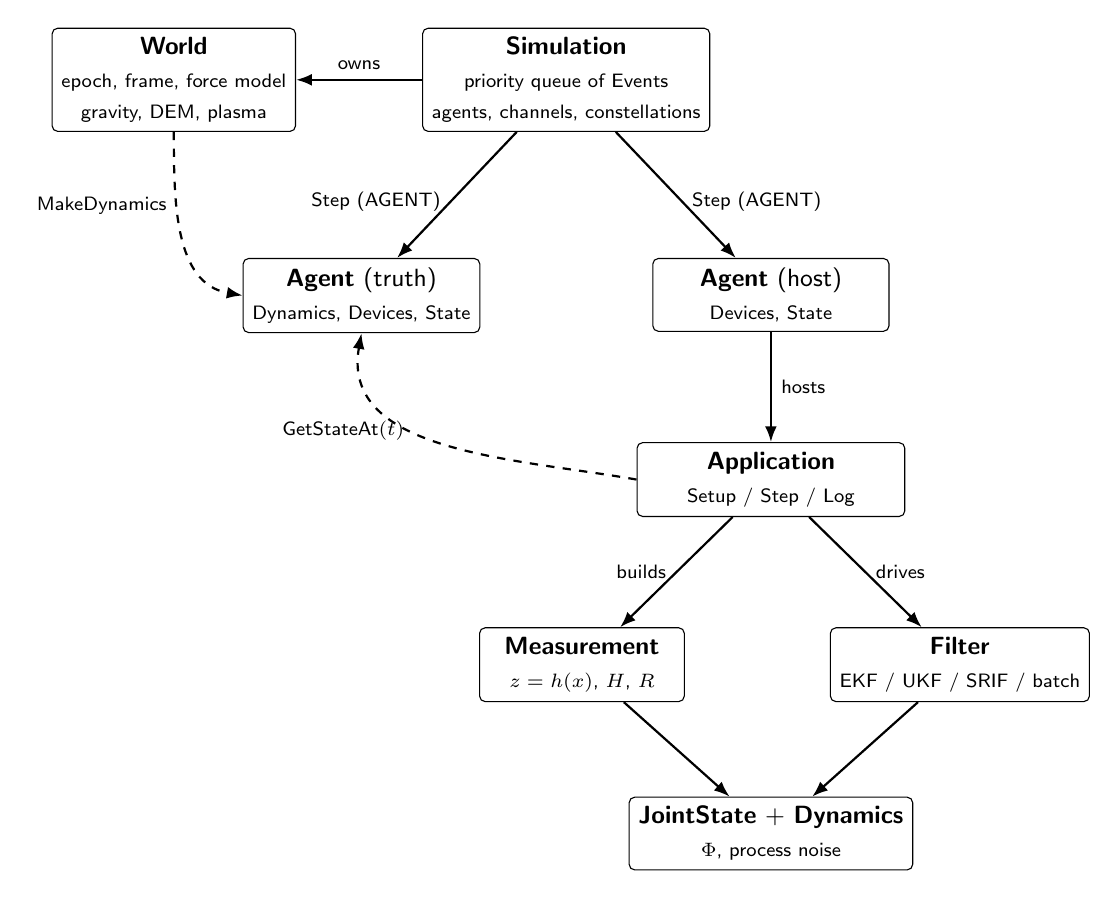
\begin{tikzpicture}[node distance=9mm and 12mm]
    % --- engine layer -------------------------------------------------------
    \node[boxnode, minimum width=3.6cm] (sim)
      {\textbf{Simulation}\\[1pt]\scriptsize priority queue of Events\\
       \scriptsize agents, channels, constellations};
    \node[boxnode, left=16mm of sim, minimum width=3.0cm] (world)
      {\textbf{World}\\[1pt]\scriptsize epoch, frame, force model\\
       \scriptsize gravity, DEM, plasma};

    % --- agent layer --------------------------------------------------------
    \node[boxnode, below=16mm of sim, xshift=-26mm, minimum width=3.0cm] (agentA)
      {\textbf{Agent} (truth)\\[1pt]\scriptsize Dynamics, Devices, State};
    \node[boxnode, below=16mm of sim, xshift=26mm, minimum width=3.0cm] (agentB)
      {\textbf{Agent} (host)\\[1pt]\scriptsize Devices, State};

    % --- application layer --------------------------------------------------
    \node[boxnode, below=14mm of agentB, minimum width=3.4cm] (app)
      {\textbf{Application}\\[1pt]\scriptsize Setup / Step / Log};

    % --- model layer --------------------------------------------------------
    \node[boxnode, below=14mm of app, xshift=-24mm, minimum width=2.6cm] (meas)
      {\textbf{Measurement}\\[1pt]\scriptsize $z=h(x)$, $H$, $R$};
    \node[boxnode, below=14mm of app, xshift=24mm, minimum width=2.6cm] (filt)
      {\textbf{Filter}\\[1pt]\scriptsize EKF / UKF / SRIF / batch};
    \node[boxnode, below=12mm of meas, xshift=24mm, minimum width=3.4cm] (state)
      {\textbf{JointState} $+$ \textbf{Dynamics}\\[1pt]\scriptsize $\Phi$, process noise};

    % --- edges --------------------------------------------------------------
    \draw[flow] (sim) -- node[above,font=\scriptsize\sffamily] {owns} (world);
    \draw[flow] (sim) -- node[left,pos=0.55,font=\scriptsize\sffamily] {Step (AGENT)} (agentA);
    \draw[flow] (sim) -- node[right,pos=0.55,font=\scriptsize\sffamily] {Step (AGENT)} (agentB);
    \draw[flow] (agentB) -- node[right,font=\scriptsize\sffamily] {hosts} (app);
    \draw[flow] (app) -- node[left,font=\scriptsize\sffamily] {builds} (meas);
    \draw[flow] (app) -- node[right,font=\scriptsize\sffamily] {drives} (filt);
    \draw[flow] (meas) -- (state);
    \draw[flow] (filt) -- (state);
    \draw[flow, dashed] (app.west) to[out=170,in=-100]
      node[left,pos=0.6,font=\scriptsize\sffamily] {GetStateAt$(t)$} (agentA.south);
    \draw[flow, dashed] (world.south) to[out=-90,in=170]
      node[left,pos=0.35,font=\scriptsize\sffamily] {MakeDynamics} (agentA.west);
  \end{tikzpicture}
  \caption{Object model and per-step call flow. Solid arrows are ownership or
           scheduling; dashed arrows are read-only queries. The engine pops due
           events, agents self-propagate their truth, devices advance, and the
           hosted application reads truth through \cpp{GetStateAt}, forms a
           measurement, and runs one filter cycle.}
  \label{fig:sim-object-model}
\end{figure}

\subsection{Simulation --- the engine}
\label{sec:sim-engine}

\cpp{Simulation} is a discrete-event engine backed by a
\cpp{std::priority\_queue<Event>}. An \cpp{Event} (\file{cpp/lupnt/core/event.h})
is a \code{\{time, frequency, priority, callback\}} tuple:

\begin{lstlisting}[language=cpp, caption={The event record and its ordering.}, label={lst:sim-event}]
// cpp/lupnt/core/event.h :: Event
struct Event {
  Real time;
  Real frequency;
  Real priority = 0.0;
  std::function<void(Real)> callback;
  bool operator<(const Event& e) const {
    return time > e.time || (time == e.time && priority > e.priority);
  }
  enum Priority {
    LOW = 0, MEDIUM = 1, HIGH = 2,
    LOGGING = LOW, APPLICATION = LOW,
    DEVICE = MEDIUM,
    DYNAMICS = HIGH, AGENT = HIGH,
  };
  constexpr static Real SINGLE_EVENT = -1.0;
};
\end{lstlisting}

The comparator inverts \cpp{operator<} on \code{time}, so the
\cpp{std::priority\_queue} (a max-heap) pops the \emph{earliest} event first ---
the intended behaviour. The tie-break on \code{priority} is written in the same
direction, so at equal time the numerically \emph{lower} priority value is popped
first: \code{APPLICATION} $=$ \code{LOGGING} $(0)$, then \code{DEVICE} $(1)$, then
\code{DYNAMICS} $=$ \code{AGENT} $(2)$.

\begin{lupntnote}
The enum names suggest the opposite intent (dynamics before devices before
applications). In practice the ordering is benign, because an application never
reads a cached agent state: \cpp{AgentWithDynamics::GetStateAt(t)} propagates a
\emph{copy} of \code{state\_} from \code{time\_} to $t$ without mutating the
agent, so the truth an application sees at time $t$ is correct whether or not the
agent's own \cpp{Step} has already fired at that epoch. Applications that depend
on a device having advanced first (an IMU sample, a clock realization) should
read the device through its own accessor rather than relying on event order.
\end{lupntnote}

The main loop pops the earliest event, sets the simulation clock, invokes the
callback, and --- if the event carries a non-zero \code{frequency} --- reschedules
it at $t + 1/f$, which is how periodic \cpp{Step} callbacks recur:

\begin{lstlisting}[language=cpp, caption={The engine loop.}, label={lst:sim-run-loop}]
// cpp/lupnt/simulations/simulation.cc :: Simulation::Run
running_ = true;
while (!queue_.empty() && queue_.top().time <= duration_ + EPS) {
  Event e = queue_.top();
  queue_.pop();
  time_ = e.time;
  e.callback(e.time);                 // Agent / Device / Application Step, or a Publish
  if (e.frequency > 0.0) {            // periodic -> reschedule
    Real time_next = e.time + 1.0 / e.frequency;
    if (time_next <= duration_ + EPS) { e.time = time_next; queue_.push(e); }
  }
}
DataLogger::Flush();
\end{lstlisting}

\cpp{Schedule(time, callback, freq, priority)} adds events. \cpp{Subscribe(topic,
callback)} and \cpp{Publish(time, topic, message)} provide a topic-based message
bus; a \cpp{Publish} does not call subscribers inline but schedules one
single-shot \code{APPLICATION}-priority event per subscriber at the given time,
which is what gives the distributed ISL scenario its one-interval message latency.
\cpp{GetAgent(name)} and \cpp{GetChannel(name)} accept either a bare name or the
fully-qualified \code{<simname>/<name>} key under which the object was registered.

\subsection{World --- the shared environment}
\label{sec:sim-world}

\cpp{Simulation::Setup} builds a single \cpp{World} from the top-level
\code{world:} block \emph{after} the epoch is set and \emph{before} any agents, so
every agent and application can pull the shared force model and truth facade
during its own \cpp{Setup}. Reach it from anywhere with \cpp{Agent::GetWorld()}
(equivalently \cpp{GetSimulation()->GetWorld()}).

The \cpp{World} recognizes the keys in \cref{tab:sim-world-keys}. All of them are
optional; a scenario with no \code{world:} block simply has
\cpp{GetWorld() == nullptr}.

\begin{table}[H]
  \centering
  \caption{Keys parsed by \cpp{World::World} in \texttt{cpp/lupnt/simulations/world.cc}.}
  \label{tab:sim-world-keys}
  \begin{tabularx}{\textwidth}{@{}l l L@{}}
    \toprule
    Key & Default & Meaning \\
    \midrule
    \code{frame} & \code{MOON\_CI} & Integration / environment reference frame. \\
    \code{force\_model} & --- & An \cpp{NBodyDynamics}-style force-model block
      (see \cref{sec:sim-force-model}); enables \cpp{MakeDynamics()},
      \cpp{MakeTruthDynamics()} and \cpp{HasForceModel()}. \\
    \code{gravity.body} & \code{MOON} & Central body whose point-mass $GM$ backs
      \cpp{Gravity(r)}, used by surface inertial-navigation mechanization. \\
    \code{dem.site\_lat\_deg}, \code{dem.site\_lon\_deg} & required in
      \code{dem:} & Site centre of the LOLA digital elevation model, and the
      origin of the local east--north--up (ENU) tangent frame. \\
    \code{dem.half\_width\_m} & \num{5000} & Half-width of the loaded DEM tile
      [\si{\meter}]. \\
    \code{dem.max\_res\_m} & \num{20} & Target DEM resolution [\si{\meter}]. \\
    \code{dem.dem\_file} & --- & Explicit GeoTIFF to crop instead of downloading
      a tile (used by tests and small fixtures). \\
    \code{plasma} & --- & Ionosphere / plasmasphere signal-delay environment; a
      shared truth property, read by the GNSS ODTS application. \\
    \bottomrule
  \end{tabularx}
\end{table}

The epoch is not a \code{world:} key: it is taken from the global \lupnt{} epoch,
which \cpp{Simulation::Setup} sets from the scenario-level \code{epoch:} string
before constructing the \cpp{World}.

Three factory methods hand out dynamics built from the one shared force model:

\begin{lstlisting}[language=cpp, caption={\cpp{World} dynamics factories.}, label={lst:sim-world-dyn}]
// cpp/lupnt/simulations/world.cc
Ptr<NBodyDynamics> World::MakeDynamics() const {        // for ESTIMATORS
  Config cfg = force_model_;
  auto dynamics = MakePtr<NBodyDynamics>(cfg);
  dynamics->SetFrame(frame_);
  dynamics->SetAutodiff(true);      // analytic state-transition matrix
  return dynamics;
}
Ptr<NBodyDynamics> World::MakeDynamics(double cr, double area_m2, double mass_kg) const;
Ptr<NBodyDynamics> World::MakeTruthDynamics() const {   // same model, SetAutodiff(false)
  auto dynamics = MakeDynamics();
  dynamics->SetAutodiff(false);     // truth propagation needs no STM
  return dynamics;
}
\end{lstlisting}

An application that reuses \cpp{MakeDynamics()} for \emph{both} the truth grid and
the filter has no truth/filter model mismatch by construction. The \cpp{World} is
strictly read-only: it \emph{provides} the environment and a truth facade
(\cpp{World::GetStateAt(name, t)}, which forwards to
\cpp{Simulation::GetAgent(name)->GetStateAt(t)}), but each
\cpp{AgentWithDynamics} still self-propagates through its own \code{dynamics\_}.

\begin{lupntnote}
An agent that declares no \code{dynamics:} block of its own inherits the shared
\code{world.force\_model} as its truth dynamics. \cpp{Simulation::Setup} injects a
copy of that block into the agent's config, defaulting \code{class} to
\code{NBodyDynamics}, inheriting \code{world.frame}, and forcing
\code{autodiff: false}. Fixed agents (ground and surface stations, which use a
\cpp{StaticDynamics}) and manager agents ignore the injected block.
\end{lupntnote}

\subsection{Agent --- a platform}
\label{sec:sim-agent}

\cpp{Agent} owns \code{name\_}, a back-pointer to the \cpp{Simulation}, a
\cpp{State}, a map of \cpp{Device}s, and one or more \cpp{Application}s. Its
pure-virtual

\begin{equation}
  \label{eq:sim-getstateat}
  \cpp{Cart6 GetStateAt(Real t) const}
  \quad\longmapsto\quad
  \vec{x}(t) = \begin{bmatrix}\vec{r}(t)\\ \vec{v}(t)\end{bmatrix}
\end{equation}

is the contract every concrete agent must answer --- \emph{``where am I at time
$t$?''} --- and is what measurement models call for light-time geometry. The
returned state is Cartesian position and velocity in the agent's dynamics frame.

Almost every physical agent derives from \cpp{AgentWithDynamics}, which adds a
\cpp{Ptr<Dynamics>}, an \cpp{AttitudeDynamics}, a \cpp{Cart6 state\_}, an
\cpp{Attitude attitude\_}, and a \cpp{State control\_}. Its \cpp{Step(t)} calls
\cpp{Propagate(t)} --- integrating the dynamics in place from \code{time\_} to $t$
with the current \code{control\_} --- and then \cpp{Log(t)}. Its
\cpp{GetStateAt(t)} returns the cached \code{state\_} if $|t - \code{time\_}| <
\code{EPS}$, and otherwise propagates a non-mutating copy.

\Cref{tab:sim-agent-classes} lists the concrete agents registered with the
factory. Applications are attached with the \code{application:} map (a single app)
or the \code{applications:} sequence (several, run in insertion order); retrieve
them with \cpp{GetApplication()}, \cpp{GetApplications()}, or
\cpp{GetApplicationByName("...")}, which matches any app whose (agent-prefixed)
name \emph{ends with} the argument.

\begin{table}[H]
  \centering
  \caption{Agent classes registered with \cpp{AgentFactory} (the string is the
           YAML \code{class:} value).}
  \label{tab:sim-agent-classes}
  \begin{tabularx}{\textwidth}{@{}l l L@{}}
    \toprule
    \code{class:} & Source & Role \\
    \midrule
    \cpp{Satellite} & \file{agents/satellite.cc} &
      Orbit-only truth from a \code{ClassicalOE} initial state; self-propagates
      its \code{dynamics:} block. \\
    \cpp{Spacecraft} & \file{agents/spacecraft.cc} &
      Joint orbit $+$ clock 8-state truth
      $[\vec{r}, \vec{v}, b, d]$ with a \code{clock:} model; accepts
      \code{r0\_m}/\code{v0\_mps} or a \code{ClassicalOE} block. \\
    \cpp{GroundStation} & \file{agents/ground_station.cc} &
      Earth station from \code{latitude\_deg} / \code{longitude\_deg} /
      \code{altitude\_m}, or from SPICE (\code{spice\_name}, \code{spice\_id},
      \code{spice\_frame}, \code{spice\_kernel(s)}). \\
    \cpp{GroundStationManager} & \file{agents/ground_station_manager.cc} &
      Massless ground-segment host for a centralized estimator application. \\
    \cpp{SurfaceStation} & \file{agents/surface_station.cc} &
      Lunar surface beacon / station. \\
    \cpp{SurfaceStationManager} & \file{agents/surface_station_manager.cc} &
      Host for the centralized ground filter in the ISL scenario. \\
    \cpp{Rover} & \file{agents/rover.cc} &
      Surface rover driven by \cpp{SurfaceDynamics2D} with a control input. \\
    \cpp{Lander} & \file{agents/lander.cc} &
      Thin descent platform; carries the guidance and navigation applications. \\
    \cpp{EphemerisManager} & \file{agents/ephemeris_manager.cc} &
      Host for the ephemeris-generation application. \\
    \cpp{LunarNavConstellation} & \file{agents/lunar_nav_constellation.cc} &
      Group generator: one \code{agents:} entry expands into $N$ child
      \cpp{Spacecraft}, from an explicit \code{satellites:} list or a symmetric
      \code{walker:} spec. \\
    \bottomrule
  \end{tabularx}
\end{table}

\cpp{LunarNavConstellation} deserves a note because it removes the need to declare
one agent per navigation satellite. Its \code{walker:} block takes
\code{n\_planes}, \code{sats\_per\_plane}, the common frozen-orbit elements
\code{a}, \code{e}, \code{i}, \code{omega}, and the phasing keys
\code{raan0\_deg}, \code{m0\_deg}, \code{phase\_deg}, plus \code{frame} (default
\code{MOON\_OP}) and \code{name\_prefix} (default \code{SV}). Right ascension of
the ascending node for plane $p$ and mean anomaly for satellite $s$ of that plane
are

\begin{align}
  \Omega_p &= \Omega_0 + p\,\frac{360^\circ}{n_\text{planes}},
  & p &= 0,\dots,n_\text{planes}-1, \label{eq:sim-walker-raan}\\
  M_{p,s} &= M_0 + s\,\frac{360^\circ}{n_\text{sat/plane}} + p\,\Delta\phi,
  & s &= 0,\dots,n_\text{sat/plane}-1, \label{eq:sim-walker-anomaly}
\end{align}

with $\Delta\phi$ the inter-plane phasing \code{phase\_deg}. The surface-rover
example sources its relay truth from such a constellation via
\cpp{GetSatelliteStateAt(j, t)}. A separate top-level \code{constellations:} block
builds \cpp{Constellation} / \cpp{GnssConstellation} objects, which are registered
and set up alongside agents.

\subsection{Application --- the mission logic}
\label{sec:sim-application}

\cpp{Application} holds a back-pointer to its owning \cpp{Agent} and a copy of its
\code{application:} config block. The base constructor reads only two keys,
\code{name} (defaulting to the object id) and \code{frequency} [\si{\hertz}];
everything else is the derived class's business. The base \cpp{Setup()} schedules
the periodic step and nothing more:

\begin{lstlisting}[language=cpp, caption={The \cpp{Application} lifecycle.}, label={lst:sim-app-lifecycle}]
// cpp/lupnt/applications/application.cc
Application::Application(Config& config) {
  name_ = config["name"] ? config["name"].as<std::string>() : GetId();
  config_ = config;
  if (config["frequency"]) frequency_ = config["frequency"].as<Real>();
}

void Application::Setup() {
  if (frequency_ > 0.0) {
    agent_->GetSimulation()->Schedule(
        0.0, [this](Real t) { Step(t); }, frequency_, Event::Priority::APPLICATION);
  } else {
    Logger::Warn(fmt::format("No frequency set for {}", name_), "Agent");
  }
}

virtual void Step(Real t) = 0;     // pure virtual: one predict/update cycle
virtual void Log(Real t);          // called from Agent::Log
\end{lstlisting}

So the three overridable virtuals are \cpp{Setup()} (resolve target agents, reach
the environment, seed the filter state and covariance, then call the base to keep
the scheduling), the pure-virtual \cpp{Step(Real t)} (one predict/update cycle),
and \cpp{Log(Real t)} (record results; \cpp{Agent::Log} forwards to it).

Logic can also be composed \emph{within} one application through the sub-application
pattern: \cpp{LunaNetSatApp} holds a \cpp{std::vector<Ptr<LunaNetSubApp>>} and fans
its \cpp{Step} out to each sub-application (\cpp{IslOdtsApp},
\cpp{EphemerisGenApp}).

\begin{table}[H]
  \centering
  \caption{Application classes registered with \cpp{ApplicationFactory}.}
  \label{tab:sim-app-classes}
  \begin{tabularx}{\textwidth}{@{}l L@{}}
    \toprule
    \code{class:} & Role \\
    \midrule
    \cpp{GroundStationTrackingApp} & Sensor on each \cpp{GroundStation}:
      visibility-gated range and range-rate, with optional troposphere,
      ionosphere, Shapiro, and solid Earth tide corrections, pushed to a manager. \\
    \cpp{GroundStationManagerApp} & Centralized batch (weighted least squares) plus
      square-root information filter (SRIF) and smoother, with configurable filter
      dynamics. \\
    \cpp{LunarGnssOdtsApp} & GNSS ODTS; calls the Monte-Carlo engine from its
      \cpp{Step}. \\
    \cpp{SatelliteOdtsApp} & Per-satellite onboard Schmidt EKF for the distributed
      ISL scenario; exchanges consider-states over publish--subscribe. \\
    \cpp{StationBeaconSensor} & Surface-station sensor pushing
      \cpp{IslStationObs} records to the ground filter. \\
    \cpp{GroundOdtsApp} & Centralized station-only EKF over every satellite's joint
      orbit $+$ clock 8-state. \\
    \cpp{EphemerisApp}, \cpp{LunaNetSatApp} & Ephemeris fitting; the latter hosts
      sub-applications (\cpp{IslOdtsApp}, \cpp{EphemerisGenApp}). \\
    \cpp{SurfaceStationApp} & Surface-station logic. \\
    \cpp{SurfaceRoverNavApp} & Rover inertial navigation aided by a
      \cpp{LunarNavConstellation}. \\
    \cpp{LanderGncApp} & Guidance / control: owns the powered-descent truth
      trajectory and writes the lander state. \\
    \cpp{LanderNavApp} & Error-state inertial navigation MEKF fusing IMU,
      altimeter, crater bearings, and LunaNet pseudoranges. \\
    \bottomrule
  \end{tabularx}
\end{table}

\subsection{Device, Measurement, Dynamics, State}
\label{sec:sim-models}

\paragraph{Device.} Created from the agent's \code{devices:} block, stored in
\cpp{Agent::devices\_} under \code{<agent>/<device>}, and stepped independently on
its own \code{DEVICE}-priority events, so its internal state is current when an
application reads it with \cpp{GetDevice(name)} (which accepts the bare or the
prefixed name). Registered devices: \cpp{Clock}, \cpp{Imu}, \cpp{Camera},
\cpp{Transmitter}, \cpp{Receiver}, \cpp{Transponder}, \cpp{GnssTransmitter},
\cpp{GnssReceiver}.

\paragraph{Measurement.} The observable contract is one method:

\begin{equation}
  \label{eq:sim-meas}
  \cpp{MeasData Compute(const State\& x, MatXd* H) const},
\end{equation}
which returns
\begin{equation}
  \label{eq:sim-meas-terms}
  \vec{z} = \vec{h}(\vec{x}), \qquad
  \mat{H} = \frac{\partial \vec{h}}{\partial \vec{x}}, \qquad
  \mat{R} = \operatorname{Cov}\!\left[\vec{z}\right].
\end{equation}

\cpp{MeasData} carries \code{timestamp}, the stacked observable \code{value}
($\vec{z}$), and \code{covariance} ($\mat{R}$, sized $n_z \times n_z$, diagonal by
convention). \code{H} is filled only when the caller passes a non-null pointer.
Derive from \cpp{MeasurementClone<Derived>}, a CRTP helper that supplies the
required polymorphic \cpp{Clone()}. \cpp{CreateFunction()} adapts the model to a
\cpp{FilterMeasurementFunction} suitable for
\cpp{Filter::SetMeasurementFunction} by capturing a \cpp{Clone()} of itself:

\begin{lstlisting}[language=cpp, caption={Adapting a measurement model to a filter.}, label={lst:sim-meas-fn}]
// cpp/lupnt/measurements/measurement.h :: Measurement::CreateFunction
virtual FilterMeasurementFunction CreateFunction() const {
  Ptr<Measurement> self = Clone();
  return [self](const State& x, MatXd* H, MatXd* R) -> VecXd {
    MeasData md = self->Compute(x, H);
    if (R != nullptr) *R = md.covariance;
    return md.value;
  };
}
\end{lstlisting}

Error-state (inertial navigation) observables use the parallel
\cpp{ErrorStateMeasurement} base instead. Its Jacobian is taken with respect to
the navigation \emph{error} state
$\delta\vec{x} = [\delta\vec{r}, \delta\vec{v}, \delta\vec{\theta},
\delta\vec{b}_a, \delta\vec{b}_g, \delta b, \delta d]$ and depends on the nominal
attitude, so the model consumes a \cpp{NavErrorContext}
($\vec{r}$, $\vec{v}$, $\mat{R}_{b \to n}$, clock bias and drift, error-state
size) rather than a flat \cpp{State}, and there is no \cpp{Filter} integration ---
the hosting application drives the Joseph-form update directly.

\paragraph{Dynamics.} The \cpp{Propagate} family is the contract. The
state-transition-matrix overload is what filters use for covariance propagation;
if a subclass does not provide one, the base computes it by automatic
differentiation. Concrete classes registered with \cpp{DynamicsFactory}:
\cpp{NBodyDynamics}, \cpp{JointOrbitClockDynamics}, \cpp{StaticDynamics},
\cpp{SurfaceDynamics2D}; \cpp{ClockDynamics} has its own registry, and
\cpp{FixedAttitudeDynamics} / \cpp{FixedPointingDynamics} register as
\cpp{AttitudeDynamics}.

\paragraph{State.} A labeled vector (\cpp{Cart6}, \cpp{ClassicalOE},
\cpp{ClockState2}, \cpp{ImuState}, \dots). \cpp{JointState} concatenates
(\cpp{State}, \cpp{Dynamics}, \cpp{ParamState}, estimation types, $\tau_q$) triples
and exposes the combined dynamics, state-transition-matrix, and process-noise
functions the \cpp{Filter} consumes --- this is how orbit $+$ clock ($+$ estimated
or consider parameters) become one filter state.

\section{Per-step data flow}
\label{sec:sim-dataflow}

At a given epoch the engine runs all due callbacks, and the following work
happens (\cref{fig:sim-object-model}):

\begin{enumerate}[leftmargin=*]
  \item \cpp{AgentWithDynamics::Step} advances each physical agent's \emph{truth}
        state by \cpp{Propagate}, then logs it.
  \item \cpp{Device::Step} advances clocks, IMUs, cameras, and radios.
  \item \cpp{Application::Step} reads other agents' truth via \cpp{GetStateAt(t)}
        or \cpp{World::GetStateAt(name, t)} and its own devices via
        \cpp{GetDevice(...)}, forms one or more \cpp{Measurement}s
        ($\vec{z}, \mat{H}, \mat{R}$), and runs a filter predict (using the
        \cpp{Dynamics} / \cpp{JointState} state-transition matrix and process
        noise) followed by an update.
  \item Results are logged through \cpp{Application::Log}, reached from
        \cpp{Agent::Log}. Periodic events reschedule themselves.
\end{enumerate}

In pseudocode, an agent step and a navigation application step are:

\begin{lstlisting}[language=cpp, caption={Truth propagation and one navigation cycle (pseudocode).}, label={lst:sim-step-pseudocode}]
// AgentWithDynamics::Step(t)          (priority AGENT) -- advance the truth state
state_, attitude_ = dynamics_.Propagate(state_, time_, t, control_);
time_ = t;  Log(t);

// A navigation Application::Step(t)   (priority APPLICATION)
for (tx : visible_transmitters(t)) {          // geometry via tx.GetStateAt(t)
  z, H, R = measurement(tx, receiver = agent_).Compute(x_hat, &H);
  stack(z, H, R);
}
filter.Predict(t);                            // x_hat, P via Dynamics/JointState STM + Q
filter.Update(z, H, R);                       // innovation, gain, covariance update
Log(t);
\end{lstlisting}

\section{Configuration and the asset factory}
\label{sec:sim-factory}

Classes are instantiated by name through \cpp{AssetFactory<Base, Config\&>}
(\file{cpp/lupnt/core/asset_factory.h}). A class opts in with one macro at file
scope:

\begin{lstlisting}[language=cpp, caption={Factory registration.}, label={lst:sim-register}]
// cpp/lupnt/core/asset_factory.h :: REGISTER_FACTORY_CLASS(BASE, DERIVED)
// registers a creator  [](Config& config) { return std::make_shared<DERIVED>(config); }
// under the string "DERIVED", via a file-scope static registrar object.

REGISTER_FACTORY_CLASS(Application, MyApp)    // at file scope in my_app.cc
\end{lstlisting}

The YAML \code{class:} value must match that string exactly; if it does not, the
factory aborts with a message listing every registered class name. Typed aliases
exist for each base: \cpp{AgentFactory}, \cpp{DeviceFactory},
\cpp{ApplicationFactory}, \cpp{DynamicsFactory}, \cpp{ChannelFactory}. Each
registry is defined in exactly one translation unit and explicitly instantiated,
so a single registry is shared across library boundaries.

\subsection{The scenario schema}
\label{sec:sim-schema}

\cpp{Simulation::Setup} reads the scenario-level keys in
\cref{tab:sim-top-keys}, in that order, then hands each \code{agents:} entry to
the factory named by its \code{class:}. The agent constructor in turn builds its
\code{dynamics:}, \code{attitude\_dynamics:}, \code{initial\_state:},
\code{devices:}, and \code{application:} (or \code{applications:}) sub-blocks
through the matching factories. Names are made unique by prefixing:
a channel, agent, or constellation named \code{X} in a simulation named \code{S}
is registered under \code{S/X}; a device \code{d} on agent \code{A} under
\code{A/d}; an application under \code{A/<name>}, defaulting to
\code{A/application} for the singular form and to \code{A/<class>} for each entry
of an \code{applications:} list.

\begin{table}[H]
  \centering
  \caption{Top-level scenario keys parsed by \cpp{Simulation::Setup}.}
  \label{tab:sim-top-keys}
  \begin{tabularx}{\textwidth}{@{}l L@{}}
    \toprule
    Key & Meaning \\
    \midrule
    \code{name} & Scenario name; also the output directory and the
      \code{<name>.h5} log file, and the registry prefix. \\
    \code{log\_level} & One of the \cpp{Logger::LogLevel} enum names
      (e.g.\ \code{DEBUG}, \code{INFO}, \code{WARNING}). \\
    \code{cesium\_port} & If present, starts a \cpp{CesiumViewer} on that port. \\
    \code{epoch} & Gregorian string, e.g.\ \code{"2027-03-01T00:00:00"}; sets the
      global \lupnt{} epoch for $t = 0$. \\
    \code{duration} & \code{HH:MM:SS(.sss)}; parsed to seconds and used as the
      event-loop horizon. \\
    \code{world} & The shared environment (\cref{tab:sim-world-keys}). \\
    \code{channels} & Map of \cpp{Channel} configs. \\
    \code{agents} & Map of agent configs, each with a \code{class:}. \\
    \code{constellations} & Map of \cpp{Constellation} configs. \\
    \code{seed} & Monte-Carlo seed, propagated as the default to every agent and
      its application. \\
    \bottomrule
  \end{tabularx}
\end{table}

An abridged scenario, from \file{configs/ground_station_odts.yaml}:

\begin{lstlisting}[language=yamlcfg, caption={A complete scenario skeleton, abridged from \texttt{configs/ground\_station\_odts.yaml}.}, label={lst:sim-yaml-gsodts}]
# configs/ground_station_odts.yaml
name: ground_station_odts
epoch: "2026-01-01T00:00:00"
duration: "36:00:00"          # 36 h (~2.7 ELFO orbits)
log_level: INFO

world:                        # shared, read-only environment
  frame: MOON_CI
  force_model:                # 2x2 Moon + Earth/Sun + SRP
    integrator: RKF45
    dt: 10.0
    max_iter: 1000
    abstol: 1.0e-6
    reltol: 1.0e-10
    autodiff: true            # analytic STM for the estimator
    mass: 10.0                # [kg]   } SRP: CR * area / mass
    area: 0.02                # [m^2]  }
    CR: 1.8
    bodies:
      - MOON: { n: 2, m: 2 }
      - EARTH: {}
      - SUN: {}

agents:
  sat:                              # truth target
    class: Satellite
    frequency: 0.0033333333333333   # 1/300 Hz truth logging
    # No `dynamics:` block -> inherits world.force_model (autodiff forced off).
    initial_state:
      class: ClassicalOE
      frame: MOON_OP
      a: 6541400.0                  # [m]
      e: 0.6
      i: 56.2                       # [deg]
      Omega: 0.0
      omega: 90.0
      M: 0.0

  gs_manager:                       # centralized OD estimator
    class: GroundStationManager
    application:
      class: GroundStationManagerApp
      target: sat
      obs_interval_s: 300.0
      seed: 42
      initial_position_sigma_m: 2000.0
      initial_velocity_sigma_mps: 0.5
      batch_max_iterations: 10
      batch_convergence_tol: 1.0e-3
      run_srif: true
      srif_use_process_noise: true
      srif_accel_psd: 3.0e-13

  DSS14:                            # a tracking station (sensor)
    class: GroundStation
    latitude_deg: 35.426456
    longitude_deg: 243.110461
    altitude_m: 1001.39
    application:
      class: GroundStationTrackingApp
      frequency: 0.0033333333333333
      target: sat                   # resolved via GetSimulation()->GetAgent("sat")
      manager: gs_manager           # where observations are pushed
      elevation_mask_deg: 10.0
      use_range: true
      use_range_rate: true
      range_sigma_m: 10.0
      range_rate_sigma_mps: 1.0e-3
      apply_troposphere: true       # Saastamoinen zenith delay + 1/sin(el) mapping
      apply_ionosphere: true        # thin-shell VTEC delay 40.3*STEC/f^2
      apply_shapiro: true           # relativistic light-time delay
      apply_solid_earth_tide: true  # degree-2 station displacement
\end{lstlisting}

\begin{lupntwarning}
\code{yaml-cpp} does not support YAML merge keys (\code{<<:}), so repeated station
blocks must be written out in full. Anchors and aliases (\code{\&id}, \code{*id})
\emph{are} supported and are used in
\file{configs/isl_odts_distributed.yaml} to share the station list across
satellites.
\end{lupntwarning}

\subsection{One force-model schema everywhere}
\label{sec:sim-force-model}

Every place that specifies an orbit force model --- the shared
\code{world: force\_model:}, a physical agent's \code{dynamics:}, and an
estimator's filter force model --- uses the \emph{same} block, parsed by
\cpp{ParseForceModelSpec} (\file{cpp/lupnt/dynamics/numerical_orbit_dynamics.cc}).
There is no separate \code{moon\_gravity\_degree\_*} / \code{include\_earth}
dialect. The keys are:

\begin{table}[H]
  \centering
  \caption{The shared force-model block.}
  \label{tab:sim-force-model}
  \begin{tabularx}{\textwidth}{@{}l L@{}}
    \toprule
    Key & Meaning \\
    \midrule
    \code{bodies} & Sequence of single-key maps \code{BODY: \{ n, m \}}. For
      \code{MOON}, \code{n}/\code{m} are the spherical-harmonic degree and order
      (default $0$, i.e.\ point mass); \code{EARTH} and \code{SUN} are third-body
      point masses and take \code{\{\}}. \\
    \code{relativity} & Enable the relativistic correction. The spelling
      \code{use\_relativity} is accepted as an alias. \\
    \code{CR}, \code{area}, \code{mass} & Solar-radiation-pressure ballistic
      coefficient $C_R A / m$; SRP is enabled only when \code{CR} is present. \\
    \code{CD} & Drag coefficient (with \code{area} and \code{mass}). \\
    \code{integrator}, \code{dt}, \code{abstol}, \code{reltol}, \code{max\_iter} &
      Integrator selection and step/tolerance controls. \\
    \code{autodiff} & Whether the model carries an analytic state-transition
      matrix. Estimators need \code{true}; truth propagation does not. \\
    \code{frame} & Reference frame; inherited from \code{world.frame} when
      omitted in an injected block. \\
    \code{units} & Optional non-dimensional unit system. \\
    \bottomrule
  \end{tabularx}
\end{table}

\subsection{Different dynamics for truth and filter}
\label{sec:sim-truth-filter}

Truth and filter dynamics are independent knobs, so a realistic orbit-determination
study can run the estimator against a deliberately mismodeled truth.

\emph{Truth} is whatever propagates the physical agent: a self-propagating
\cpp{AgentWithDynamics} integrates its own \code{dynamics:} block (or the injected
\code{world.force\_model}), and an application reads that truth through
\cpp{GetStateAt(t)} or \cpp{World::GetStateAt(name, t)}.

\emph{Filter} dynamics are built \emph{inside} the estimator \cpp{Application} ---
either by reusing \cpp{World::MakeDynamics()} or from application-specific config.
Whatever the filter uses also supplies its state-transition matrix, so keep
\code{autodiff: true} on that model.

\emph{Same model (no mismatch).} Omit the target agent's \code{dynamics:} block so
it inherits \code{world: force\_model:}, and have the application build its filter
from \cpp{World::MakeDynamics()}. This is exactly what
\file{configs/ground_station_odts.yaml} and \file{configs/sat_bearing_odts.yaml}
do.

\emph{Different models (mismatch).} Configure the two sides separately. In the
distributed ISL scenario the truth is propagated from \code{world: force\_model:}
--- inherited by every \cpp{Spacecraft} --- at $16 \times 16$ lunar gravity, while
each onboard \cpp{SatelliteOdtsApp} runs its EKF at $8 \times 8$:

\begin{lstlisting}[language=yamlcfg, caption={Deliberate truth/filter force-model mismatch.}, label={lst:sim-yaml-mismatch}]
# configs/isl_odts_distributed.yaml
world:
  force_model:                            # truth propagated at 16x16 lunar gravity
    integrator: RKF45
    dt: 60.0
    autodiff: false
    bodies:
      - MOON: { n: 16, m: 16 }
      - EARTH: {}
      - SUN: {}

# ... every Spacecraft inherits that truth force model; the onboard app filters
# coarser using the SAME force_model schema:
application:
  class: SatelliteOdtsApp
  force_model:                            # EKF runs at 8x8 -> intentional mismatch
    bodies:
      - MOON: { n: 8, m: 8 }
      - EARTH: {}
      - SUN: {}
    relativity: true
  integration_step_s: 60.0
  process_accel_sigma_mps2: 1.0e-08
\end{lstlisting}

More generally: give the truth agent a high-fidelity \code{dynamics:} block (more
third bodies, higher gravity degree and order, SRP, drag) and point the filter at
a coarser model. An estimator application can also expose the filter model as
config: \cpp{GroundStationManagerApp} accepts an optional \code{filter\_dynamics:}
block applied to \emph{both} its batch and its sequential SRIF/smoother filters,
or \code{batch\_dynamics:} / \code{sequential\_dynamics:} to set each
independently. Absent those, both inherit \code{world: force\_model:} --- truth
equals filter, the default. In a custom application, simply build two
\cpp{Dynamics} objects instead of sharing one.

\section{Authoring a new scenario}
\label{sec:sim-authoring}

The reference template is \file{configs/ground_station_odts.yaml} together with
\file{python/examples/ex7_run_odts.py}. The steps, in increasing order of effort:

\begin{enumerate}[leftmargin=*]
  \item \textbf{Add the shared environment.} Write a \code{world:} block
    (\code{frame} $+$ \code{force\_model}, or a \code{gravity:} / \code{dem:}
    block for surface scenarios). Both truth and estimator dynamics derive from
    it.
  \item \textbf{Reuse existing classes.} List \code{agents:} with
    already-registered \code{class:} values
    (\cref{tab:sim-agent-classes}), each with an \code{initial\_state:}, an
    optional \code{dynamics:} block, optional \code{devices:}, and an
    \code{application:} block. Launch with \py{pnt.Simulation(config)}. Nothing
    else is needed if the physics and the observables already exist.
  \item \textbf{New Application} --- the most common extension. Subclass
    \cpp{Application}, implement \cpp{MyApp(Config\&)}, \cpp{Setup()}, and
    \cpp{Step(Real)}; add \cpp{REGISTER\_FACTORY\_CLASS(Application, MyApp)}.
    Reference: \file{cpp/lupnt/applications/ground_station/ground_station_manager_app.cc}.
  \item \textbf{New Measurement} --- only for a new observable. Subclass
    \cpp{MeasurementClone<MyMeas>} (or \cpp{ErrorStateMeasurement}) and implement
    \cpp{Compute(const State\&, MatXd*)}. Wire it into a filter with
    \cpp{CreateFunction()}. Reference:
    \file{cpp/lupnt/measurements/crosslink_measurement.cc}.
  \item \textbf{New Dynamics} --- only for new physics. Subclass
    \cpp{NumericalDynamics} (implementing \cpp{ComputeRates}, \cpp{Propagate},
    \cpp{GetStateType}) or \cpp{Dynamics} directly, and add
    \cpp{REGISTER\_FACTORY\_CLASS(Dynamics, MyDyn)}. The state-transition matrix is
    supplied by automatic differentiation if you do not provide one.
  \item \textbf{New Agent} --- only for a new platform kind. Subclass
    \cpp{AgentWithDynamics}, implement \cpp{GetStateAt}, optionally override
    \cpp{Propagate} / \cpp{Setup}, and add
    \cpp{REGISTER\_FACTORY\_CLASS(Agent, MyAgent)}. Reference:
    \file{cpp/lupnt/agents/satellite.cc}, \file{cpp/lupnt/agents/rover.cc}.
\end{enumerate}

The skeleton of the two most common C++ extensions:

\begin{lstlisting}[language=cpp, caption={A new application and a new observable in C++.}, label={lst:sim-cpp-skeleton}]
// --- A new navigation application ---------------------------------------
class MyOdtsApp : public Application {
 public:
  MyOdtsApp(Config& cfg) : Application(cfg) {
    target_ = cfg["target"].as<std::string>();       // agent name to track
    sigma_  = cfg["range_sigma_m"].as<double>();
  }
  void Setup() override {
    Application::Setup();                            // schedules Step at frequency_
    target_agent_ = GetAgent()->GetSimulation()->GetAgent(target_);
    dyn_ = GetAgent()->GetWorld()->MakeDynamics();    // filter model, STM enabled
    // seed filter_ state x_hat_ and covariance P_ here
  }
  void Step(Real t) override {
    Cart6 x_tx = target_agent_->GetStateAt(t);       // truth geometry
    MatXd H; MyMeasurement meas(BuildConfig(x_tx));
    MeasData zHR = meas.Compute(x_hat_, &H);         // z = h(x), R, and H
    filter_.Predict(t);                              // STM + process noise
    filter_.Update(zHR.value, H, zHR.covariance);    // innovation, gain, update
    Log(t);
  }
};
REGISTER_FACTORY_CLASS(Application, MyOdtsApp)       // YAML: class: MyOdtsApp

// --- A new observable ---------------------------------------------------
class MyMeasurement : public MeasurementClone<MyMeasurement> {
 public:
  MeasData Compute(const State& x, MatXd* H = nullptr) const override {
    VecXd z(1);   z(0) = /* h(x): range, Doppler, ... */;
    if (H) { H->resize(1, x.size()); *H = /* dh/dx */; }
    return MeasData{timestamp_, z, R_};              // value, covariance
  }
};
\end{lstlisting}

\begin{lupntwarning}
\cpp{Simulation(config)} calls \cpp{Setup()} inside its constructor, so every
agent and application is fully built and set up before \cpp{Run()} is reachable.
Any state that a host must inject \emph{after} construction (for example the
lander guidance application's reference trajectory) should therefore be applied
through a lazy \cpp{Initialize} inside the application's first \cpp{Step}.
\end{lupntwarning}

\section{Working in Python}
\label{sec:sim-python}

The whole simulation lifecycle is driven from Python. A scenario is just a
\py{dict} (or a loaded YAML document), so it can be built, mutated, and swept
programmatically:

\begin{lstlisting}[language=py, caption={Composing, mutating, and running a scenario from Python.}, label={lst:sim-py-run}]
# python/examples/ex7_run_odts.py (pattern)
import copy, yaml, pylupnt as pnt

cfg = yaml.safe_load(open("configs/ground_station_odts.yaml"))
cfg["agents"]["gs_manager"]["application"]["srif_accel_psd"] = 1e-13

sim = pnt.Simulation(cfg)     # builds World + agents + apps from the `class:` keys
sim.run()                     # runs the event loop
app = sim.get_agent("gs_manager").get_application()   # downcasts to the concrete app
\end{lstlisting}

\cpp{pnt.Simulation} accepts either a path string or a config dict. The bound
surface is deliberately small: \py{run()}, \py{get\_agent(name)},
\py{get\_world()}, \py{get\_duration()}, \py{get\_time()} on the simulation;
\py{get\_name()}, \py{get\_state\_at(t)}, \py{get\_application()},
\py{get\_applications()}, \py{get\_application\_by\_name(name)}, \py{get\_world()} on
an agent; and \py{get\_epoch()}, \py{get\_frame()}, \py{has\_force\_model()},
\py{get\_gm()}, \py{gravity(r)}, the DEM accessors, and \py{get\_state\_at(name, t)}
on the world. Each concrete application binds its own result accessors in its own
binding file (\file{python/bindings/py_ground_station_odts.cc},
\file{python/bindings/py_isl_odts.cc}, and so on).

\subsection{Authoring an Application in Python}
\label{sec:sim-py-application}

\cpp{Application}, \cpp{Agent}, and \cpp{Measurement} are exposed as polymorphic
bases with \code{pybind11} trampolines (\cpp{PyApplication}, \cpp{PyAgent},
\cpp{PyMeasurement} in \file{python/bindings/py_simulation.cc}), so a pure-Python
subclass can be driven by the C++ engine with no C++ build.
\Cref{tab:sim-trampolines} gives the dispatch contract.

\begin{table}[H]
  \centering
  \caption{Python override points exposed by the trampolines in
           \texttt{python/bindings/py\_simulation.cc}.}
  \label{tab:sim-trampolines}
  \begin{tabularx}{\textwidth}{@{}l l L@{}}
    \toprule
    Base & Python method & Contract \\
    \midrule
    \py{pnt.Application} & \py{step(self, t)} & \textbf{Required.} $t$ arrives as
      a plain Python \py{float} (not an autodiff \cpp{Real}), so ordinary
      arithmetic works. \\
    & \py{setup(self)} & Optional. Call
      \py{pnt.Application.setup(self)} to keep the base's frequency-based
      scheduling of \py{step}. \\
    & \py{log(self, t)} & Optional; falls back to the C++ base. \\
    \py{pnt.Agent} & \py{get\_state\_at(self, t)} & \textbf{Required.} Must return a
      numpy 6-vector $[\vec{r}; \vec{v}]$; the trampoline checks the size. \\
    & \py{setup}, \py{step}, \py{log} & Optional; fall back to the C++ base. \\
    \py{pnt.Measurement} & \py{compute(self, x)} & \textbf{Required.} Returns the
      tuple $(\vec{z}, \mat{H} = \partial \vec{h}/\partial \vec{x}, \mat{R})$, all
      numpy. \py{evaluate(x)} runs it through the C++ base --- the same path a
      filter uses. \\
    \bottomrule
  \end{tabularx}
\end{table}

Register the class with \py{pnt.register\_application(name, cls)} and reference it
by \code{class: name} in a config. The factory constructs it as
\py{cls(config\_dict)}, where the dict is the \code{application:} block converted
recursively from YAML (integers, floats --- including scientific notation such as
\code{1.0e-8} --- booleans, strings, lists, dicts). The returned Python object is
kept alive for the simulation's lifetime and
\py{sim.get\_agent(...).get\_application()} hands back the \emph{same} object, so
results stored on \py{self} survive the run.

\begin{lstlisting}[language=py, caption={An estimator application authored entirely in Python.}, label={lst:sim-py-app}]
# python/examples/ex17_python_new_sim_example.ipynb
import numpy as np, yaml, pylupnt as pnt

def make_dyn():
    d = pnt.NBodyDynamics()
    for b in (pnt.Body.Moon(8, 8), pnt.Body.Earth(), pnt.Body.Sun()):
        d.add_body(b)
    d.set_frame(pnt.Frame.MOON_CI)
    d.set_integrator(pnt.IntegratorType.RKF45)
    d.set_autodiff(True)          # analytic STM for the filter
    return d

class PyAnglesOdtsApp(pnt.Application):
    def __init__(self, config):                      # config = the `application:` block
        pnt.Application.__init__(self)
        self.target = config["target"]
        self.set_frequency(config.get("frequency", 1.0 / 60))
        self.sigma = np.radians(config.get("angle_sigma_arcsec", 2.0) / 3600.0)
        self.p0 = config.get("initial_position_sigma_m", 300.0)
        self.v0 = config.get("initial_velocity_sigma_mps", 0.3)
        self.qa = config.get("process_accel_sigma_mps2", 1e-6)
        self.rng = np.random.default_rng(config.get("seed", 42))
        self.times, self.est, self.truth, self.sig = [], [], [], []
        self._init = False

    def setup(self):
        pnt.Application.setup(self)   # base schedules step() at get_frequency()
        self.dyn = make_dyn()
        self.meas = BearingMeasurement(self.sigma)

    def step(self, t):
        if not self._init:                                   # seed once
            self.obs = np.asarray(self.get_agent().get_state_at(0.0))
            self.tgt = np.asarray(
                self.get_agent().get_world().get_state_at(self.target, 0.0))
            self.x = self.obs + np.r_[self.rng.normal(0, self.p0, 3),
                                      self.rng.normal(0, self.v0, 3)]
            self.P = np.diag(np.r_[[self.p0**2] * 3, [self.v0**2] * 3])
            self._init, self._t = True, t
            return
        dt = t - self._t
        xf, F = self.dyn.propagate_stm(self.x, float(self._t), float(t))
        self.x = np.asarray(xf).ravel(); F = np.asarray(F); self._t = t
        Q = self.qa**2 * np.block([[dt**3 / 3 * np.eye(3), dt**2 / 2 * np.eye(3)],
                                   [dt**2 / 2 * np.eye(3), dt * np.eye(3)]])
        self.P = F @ self.P @ F.T + Q                        # predict
        self.meas.target = self.tgt[:3]
        z = self.meas.evaluate(self.obs)[0] + self.rng.normal(0, self.sigma, 3)
        u, H, R = self.meas.evaluate(self.x)                 # predict the observable
        S = H @ self.P @ H.T + R
        K = self.P @ H.T @ np.linalg.inv(S)
        self.x = self.x + K @ (z - u)                        # update
        IKH = np.eye(6) - K @ H
        self.P = IKH @ self.P @ IKH.T + K @ R @ K.T          # Joseph form
        self.times.append(t); self.est.append(self.x.copy())

pnt.register_application("PyAnglesOdtsApp", PyAnglesOdtsApp)
cfg = yaml.safe_load(open("configs/sat_bearing_odts.yaml"))
sim = pnt.Simulation(cfg); sim.run()
est = np.array(sim.get_agent("observer").get_application().est)   # results off `self`
\end{lstlisting}

The scenario it runs is \file{configs/sat_bearing_odts.yaml}, an ordinary config
whose only unusual feature is that its \code{class:} names a Python type:

\begin{lstlisting}[language=yamlcfg, caption={A config whose application class is authored in Python.}, label={lst:sim-yaml-bearing}]
# configs/sat_bearing_odts.yaml (abridged)
observer:
  class: Spacecraft
  frequency: 0.016666666666666666
  initial_state:
    class: ClassicalOE
    frame: MOON_OP
    a: 1837400.0                    # [m] ~100 km altitude circular
    e: 0.001
    i: 30.0
    Omega: 0.0
    omega: 0.0
    M: 0.0
  application:
    class: PyAnglesOdtsApp          # registered by pnt.register_application
    target: target
    frequency: 0.016666666666666666
    dt_s: 60.0
    angle_sigma_arcsec: 2.0         # star-tracker class bearing noise
    seed: 42
    force_model:                    # filter force model, same schema as world
      bodies:
        - MOON: { n: 8, m: 8 }
        - EARTH: {}
        - SUN: {}
      relativity: false
    process_accel_sigma_mps2: 1.0e-6
    initial_position_sigma_m: 300.0
    initial_velocity_sigma_mps: 0.3
\end{lstlisting}

\subsection{Authoring a Measurement in Python}
\label{sec:sim-py-measurement}

A \py{pnt.Measurement} subclass implements
\py{compute(self, x) -> (z, H, R)}. Because \py{evaluate(x)} routes through the
C++ base --- the same path a \cpp{Filter} uses --- the \emph{same} Python class
both \emph{generates} an observation (apply it to a truth state and add noise) and
\emph{predicts} one (apply it to the filter state). The bearing model of
Example~17 is the unit line of sight $\uvec{u}$ from the observer at $\vec{r}$ to a
known target at $\vec{p}$:

\begin{align}
  \vec{d} &= \vec{p} - \vec{r}, \qquad \rho = \lVert \vec{d} \rVert, \qquad
  \uvec{u} = \vec{d}/\rho, \label{eq:sim-bearing}\\
  \frac{\partial \uvec{u}}{\partial \vec{r}}
    &= -\frac{1}{\rho}\left(\mat{I}_3 - \uvec{u}\,\uvec{u}\transpose\right),
  \qquad
  \frac{\partial \uvec{u}}{\partial \vec{v}} = \mat{0}_{3\times 3},
  \qquad
  \mat{R} = \sigma^2 \mat{I}_3. \label{eq:sim-bearing-jac}
\end{align}

\begin{lstlisting}[language=py, caption={A measurement model authored in Python.}, label={lst:sim-py-meas}]
# python/examples/ex17_python_new_sim_example.ipynb
class BearingMeasurement(pnt.Measurement):
    "Unit line-of-sight (bearing) to a known target position."

    def __init__(self, sigma_rad):
        pnt.Measurement.__init__(self)
        self.sigma = sigma_rad
        self.target = np.zeros(3)    # set per-epoch to the target truth position

    def compute(self, x):            # -> (z = h(x), H = dh/dx, R)
        d = self.target - x[:3]
        rn = np.linalg.norm(d)
        u = d / rn
        H = np.zeros((3, 6))
        H[:, :3] = -(np.eye(3) - np.outer(u, u)) / rn
        return u, H, self.sigma**2 * np.eye(3)

m = BearingMeasurement(np.radians(2 / 3600))
m.target = tgt_truth[:3]
z = m.evaluate(obs_truth)[0] + rng.normal(0, m.sigma, 3)   # GENERATE from truth
u, Hx, R = m.evaluate(x_hat)                               # PREDICT at the filter state
\end{lstlisting}

\subsection{Authoring an Agent in Python}
\label{sec:sim-py-agent}

A platform whose truth trajectory is defined in Python --- an analytic ephemeris, a
scripted path --- subclasses \py{pnt.Agent}, implements \py{get\_state\_at(self, t)},
and is registered with \py{pnt.register\_agent(name, cls)}:

\begin{lstlisting}[language=py, caption={A physical platform whose truth is an analytic Python ephemeris.}, label={lst:sim-py-agent}]
class PyEphemeris(pnt.Agent):
    def __init__(self, config):
        pnt.Agent.__init__(self)
        self.a = config["radius_m"]
        self.w = (pnt.GM_MOON / self.a**3) ** 0.5
    def get_state_at(self, t):                 # must return a numpy [r; v] 6-vector
        c, s = np.cos(self.w * t), np.sin(self.w * t)
        return np.array([self.a * c, self.a * s, 0.0,
                         -self.a * self.w * s, self.a * self.w * c, 0.0])

pnt.register_agent("PyEphemeris", PyEphemeris)
# config:  {class: PyEphemeris, radius_m: 2.0e6}
\end{lstlisting}

A complete, converging example --- the angles-only orbit-determination EKF of
\cref{lst:sim-py-app} and \cref{lst:sim-py-meas}, reaching the metre level over a
\SI{6}{\hour} arc from a \SI{300}{\meter} a-priori with \SI{2}{arcsecond} bearings
--- is Example~17, \file{python/examples/ex17_python_new_sim_example.ipynb}.

\subsection{Monte-Carlo trials}
\label{sec:sim-montecarlo}

Monte-Carlo settings live at the \emph{simulation} level, not on an agent or an
application: a trial is one independent \py{pnt.Simulation} run built from a deep
copy of the config with a distinct top-level \code{seed:}, which
\cpp{Simulation::Setup} propagates as the default to every agent and every
application. \py{pnt.run\_monte\_carlo} (\file{python/pylupnt/montecarlo.py})
parallelizes across \emph{processes} --- the C++ engine stays serial, and a
\code{spawn} context gives each worker a clean interpreter so the thread-local C++
random engine starts fresh:

\begin{lstlisting}[language=py, caption={Parallel Monte-Carlo over a scenario config.}, label={lst:sim-py-montecarlo}]
# python/pylupnt/montecarlo.py
import pylupnt as pnt

def final_error(sim):                     # must be a top-level (picklable) function
    app = sim.get_agent("gs_manager").get_application()
    return float(app.est_central()[-1, 0])

summaries = pnt.run_monte_carlo(config, n_runs=16, extract=final_error,
                                n_workers=8, seed0=0, output_root="output/mc")
# trial i uses seed = seed0 + i; every nested `output_dir` key is redirected to
# <output_root>/run_<i> so parallel trials never overwrite each other.
\end{lstlisting}

For a scenario with an expensive \emph{shared} precompute, the GNSS ODTS engine
also offers an in-configuration \code{monte\_carlo\_runs:} knob (one precompute,
then \code{seed = base\_seed + i} per run); see
\file{python/examples/ex6_gnss_odts.ipynb}.

\section{Model boundaries}
\label{sec:sim-boundaries}

This section states what the YAML front end can express on its own, what still
requires code, and which behaviours are approximations of the engine rather than
of the physics.

\subsection{What the YAML front end supports}

\begin{itemize}[leftmargin=*]
  \item The full scenario skeleton: \code{name}, \code{epoch}, \code{duration},
    \code{log\_level}, \code{cesium\_port}, \code{seed}, \code{world},
    \code{channels}, \code{agents}, \code{constellations}
    (\cref{tab:sim-top-keys}).
  \item Any composition of already-registered agents, devices, dynamics,
    channels, and applications, selected by string (\cref{tab:sim-agent-classes},
    \cref{tab:sim-app-classes}); every constructor knob of those classes is a
    config key.
  \item The complete force-model specification (\cref{tab:sim-force-model}),
    used identically for the shared environment, per-agent truth, and per-filter
    fidelity --- so a truth/filter mismatch study is a pure configuration change.
  \item Multi-application platforms (\code{applications:}), constellation
    expansion (\code{walker:} or an explicit \code{satellites:} list), and
    seed-driven Monte-Carlo sweeps.
  \item Any class authored in \emph{Python} and registered with
    \py{pnt.register\_application} or \py{pnt.register\_agent} before
    \py{pnt.Simulation} is constructed --- these are indistinguishable from C++
    classes to the config.
\end{itemize}

\subsection{What still requires code}

\begin{itemize}[leftmargin=*]
  \item \textbf{New physics.} A new \cpp{Dynamics} class must be C++: there is no
    \cpp{PyDynamics} trampoline, so a Python author reuses
    \py{pnt.NBodyDynamics} (built and propagated with state-transition matrix from
    Python) rather than writing a new propagator.
  \item \textbf{New devices and channels.} \cpp{Device} and \cpp{Channel} have no
    Python trampoline either; new hardware models are C++ subclasses with
    \cpp{REGISTER\_FACTORY\_CLASS}.
  \item \textbf{Error-state observables.} \cpp{ErrorStateMeasurement} is not bound
    to Python; only the state-vector \cpp{Measurement} base is. Inertial-navigation
    observables are therefore C++.
  \item \textbf{New filters.} The \cpp{Filter} family (\cpp{EKF}, \cpp{SRIF},
    \cpp{UDUEKF}, \cpp{UDUStochasticCloningEKF}) is registered but not
    Python-subclassable; a Python application implements its own estimator in
    numpy, as \cref{lst:sim-py-app} does.
  \item \textbf{Cross-application data structures.} An application that must hand
    typed records to another (for example \cpp{IslStationObs} from
    \cpp{StationBeaconSensor} to \cpp{GroundOdtsApp}) needs a C++ struct and an
    accessor; the generic escape hatch is the \cpp{Publish} / \cpp{Subscribe} bus,
    which carries a \cpp{std::any}.
  \item \textbf{New initial-state parameterizations.} \cpp{Satellite} accepts only
    a \code{ClassicalOE} block; \cpp{Spacecraft} accepts \code{ClassicalOE} or
    explicit \code{r0\_m}/\code{v0\_mps}. Anything else is a constructor change.
\end{itemize}

\subsection{Engine approximations and expected behaviour}

\begin{itemize}[leftmargin=*]
  \item \textbf{Tie-breaking.} At equal event time the numerically lower priority
    value runs first, so applications may execute before the agents' own
    \cpp{Step} at that epoch. This is safe because \cpp{GetStateAt(t)}
    self-propagates a copy; it is \emph{not} safe for logic that assumes a device
    has already been advanced.
  \item \textbf{Horizon.} \cpp{Run} stops when the queue is empty or the next event
    exceeds \code{duration\_} $+$ \code{EPS}, and a periodic event is not
    rescheduled past that horizon. The final epoch of a run is therefore the last
    multiple of $1/f$ within the duration, not the duration itself.
  \item \textbf{Truth propagation carries no state-transition matrix.} Inherited
    world dynamics are injected with \code{autodiff: false}, and both
    \cpp{Spacecraft} and \cpp{World::MakeTruthDynamics} force it off. An
    application that needs an STM must build its own dynamics with
    \code{autodiff: true}.
  \item \textbf{The \cpp{World} is read-only and never propagates.} It provides
    the environment and the \cpp{GetStateAt} facade; every
    \cpp{AgentWithDynamics} self-propagates. There is no central integrator and no
    global synchronization of agent epochs.
  \item \textbf{Setup runs in the constructor.} There is no window between
    construction and \cpp{Run()} in which the engine will call back into a
    partially built application, so post-construction injection must be deferred
    to the first \cpp{Step}.
  \item \textbf{Determinism.} A run is reproducible for a fixed top-level
    \code{seed:} on a fixed build; parallel Monte-Carlo uses one process per trial
    precisely because the C++ random engine is thread-local, and per-trial
    \code{output\_dir} redirection is required to keep file outputs from
    colliding.
  \item \textbf{Python overhead.} A Python-authored application acquires the GIL on
    every \py{step}, \py{setup}, \py{log}, \py{get\_state\_at}, and \py{compute}
    call. This is acceptable at the \SI{1}{\per\minute} cadences used by the
    orbit-determination examples and is not appropriate for high-rate
    (\si{\kilo\hertz}) inertial mechanization, which stays in C++.
\end{itemize}

\chapter{Building the Documentation}
\label{chap:building-docs}

\lupnt{} ships two documents built from the same repository: the Sphinx
website under \file{docs/}, which combines narrative pages, the executed
tutorial notebooks, the Python API, and a Doxygen-derived C++ API; and this
LaTeX manual under \file{latex_docs/}, which carries the mathematical
specifications in full. This chapter specifies how each is produced, which
files configure it, what the build writes where, and how to extend either one.
It expands \file{docs/builddocs.rst} with the contents of
\file{docs/make\_docs.py}, \file{docs/conf.py}, \file{docs/index.rst},
\file{docs/CMakeLists.txt}, \file{docs/Doxyfile}, and the LaTeX sources
themselves.

The developer environment that supplies the toolchain --- Pixi, its tasks, and
the CI pipeline that publishes the site --- is specified in
\cref{chap:development}.

\section{The documentation toolchain}
\label{sec:bd-toolchain}

The narrative documentation and the Python API pages are written in
reStructuredText and rendered by Sphinx. The tutorial pages come from two
sources: the Python example notebooks, included through \code{nbsphinx} and
\code{nbsphinx-link}, and the C++ example programs, included with
\code{literalinclude}. The C++ API reference is generated from Doxygen
comments in the public headers and pulled into Sphinx by the Breathe and Exhale
extensions. The generated HTML is GitHub Pages-ready.

\begin{table}[H]
  \centering
  \caption{Documentation toolchain components and where they are configured.}
  \label{tab:bd-toolchain}
  \small
  \begin{tabularx}{\textwidth}{@{}l L L@{}}
    \toprule
    Component & Role & Configured in \\
    \midrule
    Sphinx           & site generator, HTML builder & \file{docs/conf.py} \\
    \code{furo}      & HTML theme (light and dark logos) & \file{docs/conf.py} \\
    \code{autodoc}, \code{autosummary}, \code{napoleon}
                     & Python API extraction, Google/NumPy docstrings & \file{docs/conf.py} \\
    \code{nbsphinx}, \code{nbsphinx-link}
                     & renders \file{.ipynb} tutorials from stored outputs
                     & \file{docs/conf.py}, \file{docs/tutorial/Python/*.nblink} \\
    Doxygen          & parses the C++ headers into XML
                     & \code{exhaleDoxygenStdin} in \file{docs/conf.py} \\
    \code{breathe}   & bridges Doxygen XML into the Sphinx C++ domain & \file{docs/conf.py} \\
    \code{exhale}    & generates the C++ API page tree & \file{docs/conf.py} \\
    \code{pandoc}    & notebook markdown conversion for \code{nbsphinx} & Pixi dependency \\
    \code{tectonic}  & builds this LaTeX manual & \file{latex_docs/build.sh} \\
    \bottomrule
  \end{tabularx}
\end{table}

The layout of \file{docs/} is:

\begin{lstlisting}[language=shell]
docs/
  index.rst              # root toctree, and the MAKE_DOCS python-api markers
  conf.py                # Sphinx configuration (incl. the Doxygen stdin config)
  make_docs.py           # the build driver invoked by `pixi run build-docs`
  make.bat               # Windows convenience wrapper around sphinx-build
  requirements.txt       # pip requirements for a non-pixi build
  Doxyfile               # standalone Doxygen config, used by docs/CMakeLists.txt
  CMakeLists.txt         # the GenerateDocs (m.css) target
  .nojekyll              # copied into the published site
  introduction.rst  getting_started.rst  development.rst  builddocs.rst
  initialization.rst  roadmap.md
  pages/                 # new_simulation, sp3_download, cross_validation,
                         #   related_publications, about.dox
  math/                  # the mathematical specification pages (index + 11 pages)
  tutorial/
    Python/              # one .nblink per python/examples/exN_*.ipynb
    C++/                 # one .rst per cpp/examples tutorial program
  _static/               # logos, background images, generated cesium scenes
  latex/                 # THIS manual (see the last section of this chapter)
\end{lstlisting}

\section{Building with Pixi}
\label{sec:bd-pixi}

One task builds everything:

\begin{lstlisting}[language=shell]
pixi run build-docs
\end{lstlisting}

The task is defined as \code{python docs/make\_docs.py} with
\code{depends-on = ["build-py"]}. The dependency matters: the Python API
generator \emph{imports} \pylupnt{} to enumerate its classes and functions, so
the compiled extension must exist. If \file{python/pylupnt/\_pylupnt*.so} is
missing --- which only happens on a manual, non-Pixi build --- build the
bindings first:

\begin{lstlisting}[language=shell]
pixi run build-py
\end{lstlisting}

\subsection{What \file{make\_docs.py} does}
\label{sec:bd-makedocs}

\file{docs/make\_docs.py} descends from the Open3D documentation driver,
modified to use Breathe and Exhale for the C++ API. Running it performs the
following steps, in order, with the working directory set to \file{docs/}:

\begin{enumerate}[leftmargin=1.6em]
  \item Create or clear the staging directory \file{docs/\_out}.
  \item Remove \file{docs/\_static/C++/build} if present.
  \item With \code{--clean} (the default), remove \file{docs/\_out},
    \file{docs/cpp\_api}, \file{docs/python\_api}, and \file{docs/\_build}.
  \item Read \file{docs/index.rst} and collect the modules to document from the
    \code{MAKE\_DOCS/python\_api/...} markers (\cref{sec:bd-pythonapi}).
  \item For every such module, generate one \file{.rst} file per class, per
    function, and one summary page per submodule, into \file{docs/python\_api}.
  \item Invoke \code{sphinx-build -b html -j <jobs> . \_out/html}. Exhale runs
    Doxygen from inside this call and generates \file{docs/cpp\_api}.
  \item With \code{--copy} (the default), delete \file{build/docs}, copy
    \file{docs/\_out/html} there, remove the \file{.doctrees} directory, and
    copy \file{docs/.nojekyll} into it.
  \item Clean the staging directories again.
\end{enumerate}

The final site is therefore the repository-level \file{build/docs} directory,
not anything under \file{docs/}. The \file{.nojekyll} marker is what makes
GitHub Pages serve generated directories whose names begin with an underscore,
such as \file{\_static}, instead of filtering them through Jekyll.

Sphinx parallelism defaults to \code{multiprocessing.cpu\_count()} and is
overridden by the environment variable \code{LUPNT\_DOCS\_JOBS}:

\begin{lstlisting}[language=shell]
LUPNT_DOCS_JOBS=4 pixi run build-docs
\end{lstlisting}

The CI \code{pages} job sets exactly this variable to \code{4}
(\cref{sec:bd-ci}).

\begin{lupntnote}
\file{make\_docs.py} hard-codes the \code{html} builder. To produce any other
output --- \code{latex}, \code{linkcheck}, \code{dirhtml} --- call
\code{sphinx-build} directly from \file{docs/}, after generating the Python API
pages at least once so the \code{python\_api/*} toctree entries resolve.
\end{lupntnote}

\subsection{Sphinx configuration}
\label{sec:bd-conf}

\file{docs/conf.py} inserts \file{<repo>/python} at the front of
\code{sys.path} so \code{import pylupnt} resolves from the source tree exactly
as it does under Pixi activation, then declares:

\begin{lstlisting}[language=py]
# docs/conf.py
extensions = [
    "sphinx.ext.autodoc",
    "sphinx.ext.autosummary",
    "sphinx.ext.napoleon",
    "breathe",
    "exhale",
    "nbsphinx",
    "nbsphinx_link",
]

html_theme = "furo"
html_title = "LuPNT"
html_static_path = ["_static"]
html_favicon = "_static/lupnt_mark.svg"
html_theme_options = {
    "light_logo": "lupnt_logo_horizontal.svg",
    "dark_logo": "lupnt_logo_horizontal_dark.svg",
}

autodoc_default_options = {
    "members": True,
    "undoc-members": True,
    "inherited-members": True,
}
autosummary_generate = True
napoleon_google_docstring = True
napoleon_numpy_docstring = True
nbsphinx_execute = "never"

primary_domain = "cpp"
highlight_language = "cpp"
\end{lstlisting}

Because \code{primary\_domain} and \code{highlight\_language} are both
\code{cpp}, an unqualified code role or code block in a \file{.rst} page is
interpreted and highlighted as C++; Python snippets must say so explicitly.

\subsection{The C++ API: Breathe and Exhale}
\label{sec:bd-cppapi}

Exhale, not the committed \file{docs/Doxyfile}, drives the Doxygen run used by
the website. \code{exhaleUseDoxyfile} is \code{False} and
\code{exhaleExecutesDoxygen} is \code{True}, so the configuration is supplied
inline:

\begin{lstlisting}[language=py]
# docs/conf.py
breathe_projects = {"lupnt": str(DOCS_DIR / "_build" / "doxygen" / "xml")}
breathe_default_project = "lupnt"

exhale_args = {
    "containmentFolder": "./cpp_api",
    "rootFileName": "cpp_library_root.rst",
    "rootFileTitle": "C++ API",
    "doxygenStripFromPath": str(REPO_ROOT / "cpp" / "lupnt"),
    "createTreeView": True,
    "exhaleExecutesDoxygen": True,
    "exhaleUseDoxyfile": False,
    "exhaleDoxygenStdin": """
PROJECT_NAME = LuPNT
INPUT = <repo>/cpp/lupnt
RECURSIVE = YES
FILE_PATTERNS = *.h
EXCLUDE_PATTERNS = */environment/plasma/fortran/*
GENERATE_XML = YES
GENERATE_HTML = NO
GENERATE_LATEX = NO
XML_OUTPUT = xml
EXTRACT_ALL = YES
EXTRACT_ANON_NSPACES = NO
HIDE_UNDOC_MEMBERS = NO
HIDE_UNDOC_CLASSES = NO
QUIET = YES
""",
}
\end{lstlisting}

Two of these settings encode deliberate decisions:

\begin{itemize}[leftmargin=1.4em]
  \item \code{FILE\_PATTERNS = *.h} with \code{EXTRACT\_ANON\_NSPACES = NO}
    documents only the public headers. Implementation files hold internal
    anonymous-namespace helpers that Doxygen would otherwise surface as
    \code{lupnt::@<number>} namespaces in the API listing; the public API lives
    in the headers.
  \item \code{EXCLUDE\_PATTERNS} drops
    \file{cpp/lupnt/environment/plasma/fortran}, whose legacy fixed-form
    Fortran sources are not meaningfully documentable by Doxygen.
\end{itemize}

The generated pages land in \file{docs/cpp\_api}, rooted at
\file{cpp\_api/cpp\_library\_root.rst}, and the Doxygen XML in
\file{docs/\_build/doxygen/xml}. Both are regenerated from scratch on every
build and are removed by the clean steps of \cref{sec:bd-makedocs}, so neither
is committed.

To document a new C++ symbol on the website, no documentation file is needed:
add a Doxygen comment to its declaration in a header under \file{cpp/lupnt},
and it appears in the tree on the next build.

\subsection{The Python API pages}
\label{sec:bd-pythonapi}

Which Python modules get API pages is declared in a comment block inside
\file{docs/index.rst}. \file{make\_docs.py} parses lines matching
\code{MAKE\_DOCS/python\_api/<module> <type>}; the optional second field is
\code{python\_only} for pure-Python modules, and is omitted for
pybind11-backed ones. The distinction changes the member-discovery rule:
\code{python\_only} modules are scanned for classes and functions whose
\code{\_\_module\_\_} equals the module name, while binding modules are scanned
for classes belonging to the module or a submodule and for built-in functions.

\begin{lstlisting}[language=py]
# docs/index.rst (inside a comment block)
MAKE_DOCS/python_api/pylupnt
MAKE_DOCS/python_api/pylupnt.plot python_only
MAKE_DOCS/python_api/pylupnt.core.pylupnt_utils python_only
MAKE_DOCS/python_api/pylupnt.plasma.kp_loader python_only
\end{lstlisting}

The same four modules are listed again, without the marker prefix, in the
\emph{Python API} toctree so that the generated pages are actually reachable:

\begin{lstlisting}[language=py]
# docs/index.rst
.. toctree::
    :maxdepth: 1
    :caption: Python API

    python_api/pylupnt
    python_api/pylupnt.plot
    python_api/pylupnt.core.pylupnt_utils
    python_api/pylupnt.plasma.kp_loader
\end{lstlisting}

Adding a module to the Python API therefore requires editing both places: the
marker block (so the pages are generated) and the toctree (so they are linked).
Forgetting the first yields a broken toctree entry; forgetting the second
yields orphaned pages and a Sphinx warning.

\subsection{The site toctrees}

\file{docs/index.rst} groups the pages into four captioned toctrees, plus the
Python and C++ API ones above:

\begin{table}[H]
  \centering
  \caption{Top-level structure of \file{docs/index.rst}.}
  \label{tab:bd-toctrees}
  \small
  \begin{tabularx}{\textwidth}{lL}
    \toprule
    Caption & Entries \\
    \midrule
    Getting Started & \file{introduction}, \file{getting\_started},
      \file{development}, \file{pages/new\_simulation}, \file{builddocs},
      \file{pages/sp3\_download}, \file{pages/cross\_validation} \\
    Tutorial & \file{tutorial/Python/index}, \file{tutorial/C++/index},
      \file{pages/related\_publications} \\
    Math Specs & \file{math/index} \\
    Python API / C++ API & the generated trees of
      \cref{sec:bd-pythonapi,sec:bd-cppapi} \\
    \bottomrule
  \end{tabularx}
\end{table}

This is the same ordering the LaTeX manual follows in its four parts, so a page
added to one document has an obvious home in the other.

\section{Previewing locally}
\label{sec:bd-preview}

Serve the generated site rather than opening the HTML files from disk:

\begin{lstlisting}[language=shell]
python -m http.server 8000 --directory build/docs
\end{lstlisting}

then open \url{http://localhost:8000}. A local server is required for in-page
search and for the interactive visualizations to load; opening
\file{build/docs/index.html} directly leaves both broken because of the
browser's file-origin restrictions.

\section{Tutorial outputs}
\label{sec:bd-notebooks}

\code{nbsphinx} is configured with \code{nbsphinx\_execute = "never"}. The
rendered notebooks therefore display the outputs \emph{stored in} each
\file{.ipynb}; the documentation build never re-runs them. This is a
deliberate trade: the docs build stays fast and needs no runtime data bundle,
at the cost of the stored outputs being a committed artefact that can go stale.

After changing an example, or an API an example depends on, refresh those
stored outputs in place:

\begin{lstlisting}[language=shell]
pixi run render-notebooks                 # all notebooks
pixi run render-notebooks -- --only ex16  # a subset
pixi run render-tutorials                 # render, then optimize the PNGs
\end{lstlisting}

The \code{nbstripout} pre-commit hook is configured to preserve outputs for
exactly these files (\file{python/examples/exN\_*.ipynb}) and to strip every
other notebook in the repository; see \cref{sec:dev-style}.

Three classes of output behave differently once published:

\begin{itemize}[leftmargin=1.4em]
  \item \textbf{Static Matplotlib figures} are embedded as images and always
    render, offline included.
  \item \textbf{Plotly figures} (examples \code{ex12}, \code{ex14} through
    \code{ex16}) pull \code{plotly.js} from a CDN at view time, so a network
    connection is required to see them.
  \item \textbf{Cesium scenes} (example \code{ex13}) are written as
    self-contained HTML into \file{docs/\_static/cesium\_scenes} and linked
    from the page; they pull CesiumJS from a CDN.
\end{itemize}

The headless-Chrome prerequisite for the static Plotly renders, and the
system libraries it needs on a minimal Linux image, are documented in
\cref{sec:dev-notebooks}.

\section{Manual build without Pixi}
\label{sec:bd-manual}

If Pixi is not available, build the C++ library and the Python bindings first
(\cref{sec:dev-bindings}), then install the documentation dependencies and run
the driver:

\begin{lstlisting}[language=shell]
cd docs
pip install -r requirements.txt
brew install doxygen pandoc          # macOS
sudo apt-get install doxygen pandoc  # Linux
python make_docs.py
\end{lstlisting}

\file{docs/requirements.txt} lists \code{notebook}, \code{sphinx},
\code{sphinx-rtd-theme}, \code{furo}, \code{exhale}, \code{breathe},
\code{nbsphinx}, \code{nbsphinx-link}, \code{jinja2}, and
\code{lxml\_html\_clean}; Doxygen and pandoc are not pip-installable and must
come from a system package manager or conda-forge. As with the Pixi build, the
generated HTML is written to the repository-level \file{build/docs} folder.

\begin{lupntwarning}
A manual build must be able to \code{import pylupnt}. Either run it inside a
shell where \code{PYTHONPATH} contains \file{python/}, or install the package;
otherwise the Python API generation step of \cref{sec:bd-makedocs} raises an
import error before Sphinx is ever invoked.
\end{lupntwarning}

\section{The standalone Doxygen target}
\label{sec:bd-doxygen}

Independently of the Sphinx site, \file{docs/CMakeLists.txt} defines a
\code{lupnt\_docs} CMake project with a \code{GenerateDocs} target that renders
Doxygen through \code{m.css} for a standalone, more richly styled C++ reference:

\begin{lstlisting}[language=shell]
cmake -S docs -B build-docs-cmake -GNinja
cmake --build build-docs-cmake --target GenerateDocs
\end{lstlisting}

The project fetches \code{mosra/m.css} at a pinned commit through CPM, adds the
\file{cpp} project as a dependency, configures \file{docs/Doxyfile} and
\file{docs/conf.py} into the binary directory, and runs
\code{m.css/documentation/doxygen.py} on the configured \file{conf.py},
writing to \code{<binary dir>/doxygen}. The variables substituted into the
\file{Doxyfile} are \code{DOXYGEN\_PROJECT\_NAME},
\code{DOXYGEN\_PROJECT\_VERSION}, \code{DOXYGEN\_PROJECT\_ROOT}, and
\code{DOXYGEN\_OUTPUT\_DIRECTORY}.

\begin{lupntnote}
The committed \file{docs/Doxyfile} (project name \code{"LuPNT (C++ API)"},
\code{OUTPUT\_DIRECTORY = doxygen}) is used by this target only. The website's
C++ API uses the inline Doxygen configuration of \cref{sec:bd-cppapi} instead,
so changing the \file{Doxyfile} has no effect on \code{pixi run build-docs}.
\end{lupntnote}

\section{Publishing from CI}
\label{sec:bd-ci}

The \code{pages} job in \file{.github/workflows/} is the only job in the
\code{docs} stage and runs only on the default branch:

\begin{lstlisting}[language=yamlcfg]
# .github/workflows/
pages:
  extends: .build_template
  stage: docs
  variables:
    LUPNT_DOCS_JOBS: "4"
  script:
    - *download_lupnt_data
    - pixi run build-docs
    - rm -rf public
    - mv build/docs public
  artifacts:
    paths:
      - public
  rules:
    - if: '$CI_COMMIT_BRANCH == $CI_DEFAULT_BRANCH'
\end{lstlisting}

It downloads the runtime data bundle first, because \code{build-docs} depends
on \code{build-py} and the import of \pylupnt{} performed by the Python API
generator touches data paths. The site is then renamed to \file{public}, which
is where GitHub Pages expects it, and published as a job artifact. The
\file{.nojekyll} file that \file{make\_docs.py} copies makes the same tree
serve correctly from GitHub Pages.

\section{This manual: \file{latex_docs}}
\label{sec:bd-latex}

The LaTeX manual is a separate document with a separate build, and it lives at
the repository root rather than under \file{docs/}. That placement is
deliberate: the manual is a self-contained reference, so \file{docs/} may
eventually be retired, and the manual is designed to survive that. It reads nothing from \file{docs/} --- the
\code{\textbackslash graphicspath} entry for \file{docs/_static} is an optional
fallback, not a dependency.

It carries the mathematical specifications as full derivations, unit contracts,
and inline implementing code, together with the bibliography behind the models
--- of which the primary reference is \citep{iiyama2026thesis}. What only the
Sphinx site provides is the auto-generated API reference and the executed
notebooks; those are generated artefacts and are not duplicated here.

\subsection{Layout}

\begin{table}[H]
  \centering
  \caption{Files under \file{latex_docs}.}
  \label{tab:bd-latex-layout}
  \small
  \begin{tabularx}{\textwidth}{lL}
    \toprule
    Path & Role \\
    \midrule
    \file{lupnt.tex}    & the master document: class options, title page, front
      matter, the four \code{\textbackslash part} divisions, and one
      \code{\textbackslash include} per chapter \\
    \file{preamble.tex} & every package, listing style, TikZ style, admonition
      environment, and macro available to a chapter --- the only place
      \code{\textbackslash usepackage} may appear \\
    \file{chapters/}    & one \file{.tex} fragment per chapter, each
      \code{\textbackslash include}d by \file{lupnt.tex} \\
    \file{refs.bib}     & the bibliography database; the only source of
      citation keys \\
    \file{build.sh}     & the build driver; also resolves
      \code{LUPNT\_DATA\_PATH} and writes \file{figpath.tex} \\
    \file{STYLE.md}     & the chapter style contract every fragment must follow \\
    \file{build/}       & generated output, including \file{build/lupnt.pdf} \\
    \bottomrule
  \end{tabularx}
\end{table}

\subsection{Building}

No system LaTeX installation is required. \file{build.sh} uses \code{tectonic},
which downloads the packages it needs on demand and runs BibTeX itself, so a
single invocation produces a document with resolved citations and cross
references:

\begin{lstlisting}[language=shell]
cd latex_docs
./build.sh            # full build into ./build
./build.sh --keep     # keep .aux/.bbl intermediates for debugging
\end{lstlisting}

The script prefers a \code{tectonic} already on \code{PATH} and otherwise falls
back to \code{pixi exec}, which fetches it into a throwaway environment ---
nothing is added to \file{pixi.toml} or the lockfile:

\begin{lstlisting}[language=shell]
# latex_docs/build.sh, in effect
if command -v tectonic >/dev/null 2>&1; then
  RUNNER=(tectonic)
elif command -v pixi >/dev/null 2>&1; then
  RUNNER=(pixi exec --spec tectonic tectonic)
fi
"${RUNNER[@]}" --outdir build lupnt.tex
\end{lstlisting}

Without the \code{--keep} flag the script deletes the \code{.aux}, \code{.log},
\code{.out}, \code{.toc}, \code{.bbl}, \code{.blg}, and \code{.bcf}
intermediates, leaving only \file{build/lupnt.pdf}. Equivalent invocations, if
either tool is preferred directly:

\begin{lstlisting}[language=shell]
# tectonic, directly
tectonic --outdir build lupnt.tex

# or a classic TeX Live toolchain
pdflatex lupnt && bibtex lupnt && pdflatex lupnt && pdflatex lupnt
\end{lstlisting}

\begin{lupntnote}
\file{refs.bib} must sit beside \file{lupnt.tex}, which is why it is committed
in \file{latex_docs} rather than generated or symlinked from elsewhere:
tectonic resolves the bibliography relative to the main file.
\end{lupntnote}

The manual is not built by \code{pixi run build-docs} and is not published by
the \code{pages} job. It is built on demand.

\subsection{Adding a chapter}
\label{sec:bd-newchapter}

Three steps, in order:

\begin{enumerate}[leftmargin=1.6em]
  \item Write \file{latex_docs/chapters/foo.tex} as a \emph{fragment}. It must
    not contain \code{\textbackslash documentclass},
    \code{\textbackslash usepackage}, \code{\textbackslash begin\{document\}},
    or a bibliography --- \file{preamble.tex} has already been read by the time
    the fragment is included. It opens with a
    \code{\textbackslash chapter\{...\}} and its label:
\begin{lstlisting}
% latex_docs/chapters/foo.tex
\chapter{Time Systems and Conversions}
\label{chap:time-conversions}

Opening paragraph: what this chapter specifies, which source files
implement it, and which references it follows.

\section{...}
\label{sec:tc-...}
\end{lstlisting}
  \item Add \code{\textbackslash include\{chapters/foo\}} to
    \file{lupnt.tex}, inside the \code{\textbackslash part} it belongs to. The
    order of the \code{\textbackslash include} lines is the order of the
    document; there is no separate table of contents to maintain.
  \item Follow \file{STYLE.md}. It is the contract, not a suggestion; the
    points it fixes are summarised below.
\end{enumerate}

If a new package is genuinely needed, add it to \file{preamble.tex} rather than
to the chapter, so that every chapter stays compilable in isolation via
\code{\textbackslash includeonly}.

\subsection{The style contract in brief}

\file{STYLE.md} is authoritative; this is an index of what it fixes.

{\small
  \begin{longtable}{@{}>{\raggedright\arraybackslash}p{0.40\textwidth}
                      >{\raggedright\arraybackslash}p{0.54\textwidth}@{}}
    \caption{Macros and environments a chapter may use, from
             \file{preamble.tex}.}
    \label{tab:bd-style} \\
    \toprule
    Construct & Use for \\
    \midrule
    \endfirsthead
    \toprule
    Construct & Use for \\
    \midrule
    \endhead
    \bottomrule
    \endlastfoot
    \code{\textbackslash code\{x\}} & identifier, enum value, CLI flag, short
      expression \\
    \code{\textbackslash cpp\{X\}}, \code{\textbackslash py\{x\}} & a C++ or
      Python symbol \\
    \code{\textbackslash file\{cpp/lupnt/x.cc\}} & a repository path (breaks at
      \code{/} and the underscore) \\
    \code{\textbackslash lupnt\{\}}, \code{\textbackslash pylupnt\{\}} & the
      library name, the Python package \\
    \code{\textbackslash vec}, \code{\textbackslash mat},
      \code{\textbackslash uvec} & 3-vector, matrix, unit vector \\
    \code{\textbackslash dd}, \code{\textbackslash transpose} & upright
      differential, transpose superscript \\
    \code{\textbackslash diag}, \code{\textbackslash atantwo},
      \code{\textbackslash argmin}, \code{\textbackslash Tr},
      \code{\textbackslash erf} & operators \\
    \code{\textbackslash TT}, \code{\textbackslash TAI},
      \code{\textbackslash TDB}, \ldots & time scales, in math mode \\
    \code{\textbackslash SI}, \code{\textbackslash si},
      \code{\textbackslash num} & units, via \code{siunitx}; extra units
      \code{\textbackslash yr}, \code{\textbackslash dayunit},
      \code{\textbackslash bit}, \code{\textbackslash dB},
      \code{\textbackslash dBHz}, \code{\textbackslash dBW},
      \code{\textbackslash dBi}, \code{\textbackslash TECU},
      \code{\textbackslash au} \\
    \code{lupntnote}, \code{lupntwarning} & replace the reStructuredText
      \code{.. note::} and \code{.. warning::} \\
    \code{lstlisting} & languages \code{cpp}, \code{py}, \code{yamlcfg},
      \code{shell}, \code{bibtexlang} \\
    \code{booktabs}, \code{tabularx} with the ragged-right \code{L} column &
      tables \\
    TikZ styles \code{tsnode}, \code{boxnode} and edge classes
      \code{constant}, \code{table}, \code{linear}, \code{model},
      \code{integral}, \code{flow} & diagrams \\
  \end{longtable}
}

Four rules are easy to violate and worth restating:

\begin{itemize}[leftmargin=1.4em]
  \item \textbf{Labels are prefixed by kind and scope}: \code{chap:<slug>},
    \code{sec:<slug>-<name>}, \code{eq:<slug>-<name>},
    \code{tab:<slug>-<name>}, \code{fig:<slug>-<name>},
    \code{lst:<slug>-<name>}. Reference them with
    \code{\textbackslash cref} or \code{\textbackslash Cref}, never with a
    hard-coded number.
  \item \textbf{Citations use keys that already exist in \file{refs.bib}}. Add
    an entry rather than inventing a key. Chapter and equation numbers in the
    thesis are cited as
    \code{\textbackslash citep[Ch.~6.2]\{iiyama2026thesis\}}.
  \item \textbf{Listings are ASCII only} --- no arrows, Greek letters, or en
    dashes --- and every listing names the file it came from on its first
    line. The same applies to prose: non-ASCII characters belong in math mode,
    as \code{\$\textbackslash mu\$} or \code{\$\textbackslash approx\$}, never
    bare.
  \item \textbf{Chapters are specifications, not summaries.} Each model states
    the state, unit, and time-scale contract it assumes; the governing
    equations, numbered, with every symbol defined; the implementing code with
    its source path; the configuration knobs that change its behaviour; and an
    explicit \emph{model boundaries} section covering what is approximated,
    what is omitted, and what accuracy is expected.
\end{itemize}

\subsection{Keeping the two documents consistent}

The Sphinx site and this manual are written from the same repository but are
not generated from one another. Consequences worth planning around:

\begin{itemize}[leftmargin=1.4em]
  \item A change to a \file{.rst} page does not propagate to the corresponding
    chapter, and vice versa. The mapping is one chapter per page, with the
    filenames deliberately kept parallel
    (\file{docs/development.rst} $\leftrightarrow$
    \file{latex_docs/chapters/development.tex}).
  \item The manual has no CI job. A LaTeX error is caught only when someone
    runs \file{build.sh}; there is no equivalent of the \code{pages} job to
    fail the pipeline.
  \item Undefined cross references and missing citations are warnings, not
    errors, under tectonic. Check the build log for
    \code{LaTeX Warning: Reference ... undefined} and
    \code{Citation ... undefined} before considering a chapter finished.
  \item Notebook outputs and the API references appear only on the website. The
    manual draws its own figures in TikZ instead, so that they add no binary
    weight to the repository and cannot drift out of sync with the prose.
  \item \file{latex_docs} is \textbf{text only}; its \file{.gitignore} rejects
    images and PDFs. Assets shared with the Sphinx site are read from
    \file{docs/_static}, and generated or large artefacts from
    \file{\$LUPNT_DATA_PATH/docs}, included with \code{\textbackslash datafig}
    so that a clone without the fetched data directory still builds --- the
    figure degrades to a placeholder rather than failing.
\end{itemize}


% ===========================================================================
\part{Tutorials}
\label{part:tutorials}
% ===========================================================================

\chapter{Tutorials}
\label{chap:tutorials}

This chapter walks through the worked examples that ship with \lupnt{}. Every
example exists in two forms: a Python notebook under \file{python/examples/},
which renders the results as 3-D scenes, time histories, maps and histograms,
and --- for most of them --- a standalone C++ program under
\file{cpp/examples/tutorials/} that computes the same quantities and prints them
as console statistics. The two are deliberately kept numerically equivalent: the
notebook is the exploratory surface, the \code{.cc} file is the
compile-time-checked twin that exercises the same library entry points from
C++.

The chapter is organised as one section per example. Each section states the
scenario the example configures --- epochs, orbital elements, constellations,
station sets, sensor noise --- with the actual numbers taken from the notebook;
walks through the computation with excerpts of the real source; then describes
\emph{what the example produces}: every figure it draws, what is on each axis,
the magnitudes involved, and the conclusion the reader is meant to draw. Each
section closes with a pointer to the Part~\ref{part:math} chapter that specifies
the underlying model. A consolidated index is given in
\cref{tab:tut-examples}, and \cref{sec:tut-publications} maps the examples onto
the publications whose methodology they implement.

\begin{lupntnote}
The examples are not unit tests. They are allowed to download data, to take
minutes to run, and to print approximate numbers. Every numeric result quoted in
this chapter is the value stored in the committed notebook output for one
particular run on one particular machine; a re-run with a different random seed,
a different SP3 vintage, or a different Earthdata snapshot will move the last
digits. The authoritative statements about accuracy live in the
Part~\ref{part:math} chapters and in the validation material of
Part~\ref{part:verification}.
\end{lupntnote}

% ===========================================================================
\section{Running the Examples}
\label{sec:tut-running}

Both flavours are driven by the \code{pixi} workspace defined in
\file{pixi.toml} at the repository root. The workspace's activation block sets
the environment variables the examples assume --- \code{LUPNT\_DATA\_PATH}
pointing at \file{data/LuPNT_data}, \code{PYTHONPATH} pointing at
\file{python/}, \code{PECSIMPY\_BASE\_PATH} at the plasma data, and
\code{LUPNT\_OUTPUT\_PATH} at \file{output/} --- so no manual export is needed
as long as commands are run through \code{pixi run}.

\subsection{Python notebooks}
\label{sec:tut-running-python}

The notebooks import \pylupnt{}, the pybind11 binding layer, which must be built
once. Building the bindings and registering a Jupyter kernel that inherits the
workspace environment is a single task each:

\begin{lstlisting}[language=shell, caption={Building and running the Python examples.}, label={lst:tut-run-python}]
# from the repository root
pixi run build-py         # builds the pylupnt-dev extension module
pixi run install-kernel   # registers a Jupyter kernel with LUPNT_DATA_PATH baked in

# then open any notebook with the "LuPNT (pixi)" kernel, e.g.
#   python/examples/ex1_propagate_orbit.ipynb

# or execute them headlessly and get a pass/fail summary
pixi run run-notebooks -- --only ex1 --timeout 600
pixi run run-notebooks                      # all of ex1 .. ex17
\end{lstlisting}

Every notebook begins with the same defensive preamble: it walks up from the
working directory until it finds \file{python/pylupnt/__init__.py}, puts that
\file{python/} first on \code{sys.path}, and pins \code{LUPNT\_DATA\_PATH} to the
sibling \file{data/LuPNT_data}. This makes a notebook use \emph{this} checkout's
bindings and data even when a stale copy sits on a global \code{PYTHONPATH} or
in an old kernelspec.

\code{run-notebooks} executes each notebook end-to-end without writing outputs
back. The companion task \code{render-notebooks} executes them \emph{in place},
so that the Sphinx build (which never re-executes notebooks) shows real results;
\code{render-tutorials} additionally optimises the embedded figures. Several of
the heavier examples (\cref{sec:tut-ex6}, \cref{sec:tut-ex7},
\cref{sec:tut-ex8}, \cref{sec:tut-ex9}, \cref{sec:tut-ex10},
\cref{sec:tut-ex11}) delegate the expensive run to a sibling
\code{ex*\_run\_*.py} script and let the notebook read back the exported results,
which keeps the rendered tutorial fast. Those scripts seed their output
directory from a shipped copy under \file{data/LuPNT_data/examples/}, so the
notebook still plots real numbers on a machine that has never run the
simulation.

\subsection{C++ tutorial binaries}
\label{sec:tut-running-cpp}

The directory \file{cpp/examples/} is its own CMake project, \code{lupnt\_examples}.
Its \file{CMakeLists.txt} globs every \code{.cc} file under \file{tutorials/},
turns each into an executable named after the file stem, links it against
\code{lupnt::lupnt} plus TBB, and collects them all under a convenience target
\code{all\_examples}:

\begin{lstlisting}[language=shell, caption={Building and running the C++ examples.}, label={lst:tut-run-cpp}]
# configures cpp/examples into build-examples-pixi and builds the all_examples target
pixi run build-examples

# each .cc becomes its own binary; run it FROM THE REPOSITORY ROOT, because the
# YAML-driven examples default to a relative config path such as configs/...
./build-examples-pixi/ex1_propagate_orbit
./build-examples-pixi/ex7_groundstation_odts
./build-examples-pixi/ex7_groundstation_odts configs/my_variant.yaml
\end{lstlisting}

Every YAML-driven example takes an optional first argument overriding the
configuration file, so a scenario variant can be tried without recompiling.

\subsection{Data prerequisites}
\label{sec:tut-running-data}

The Earth-GNSS examples --- \cref{sec:tut-ex3}, \cref{sec:tut-ex5}, and
\cref{sec:tut-ex6} --- are data-driven. They read SP3 precise-ephemeris
products, and in places ANTEX antenna files and RINEX broadcast navigation
messages, which are fetched from NASA CDDIS and require a free Earthdata login
(a \file{~/.netrc} entry, or the \code{EARTHDATA\_USERNAME} and
\code{EARTHDATA\_PASSWORD} environment variables). The download procedure is
specified in \cref{chap:sp3-download}. Downloads are cached under
\file{output/gnss_files/}, so only the first run needs the network.

\begin{lupntwarning}
\code{pixi run build-examples} only \emph{compiles} the programs; the data is
loaded at run time. Each of the three guards its inputs: with the files or
credentials absent it prints an informative note and exits with status zero, so
it always builds and runs, and produces its full analysis once the data is
present. \cref{sec:tut-ex6} additionally requires the staged link and
plasma-delay precompute produced by \file{python/examples/ex6_precompute.py}.
\end{lupntwarning}

\subsection{Where the figures in this chapter come from}
\label{sec:tut-running-figures}

The notebooks are committed \emph{with} their outputs --- \code{nbstripout} is
configured in this repository to preserve them --- so every plot a tutorial
produces already sits in the notebook JSON as a base64 \code{image/png} output.
\file{latex_docs/} is a text-only tree, so those images cannot be committed
beside this chapter. They are extracted instead:

\begin{lstlisting}[language=shell, caption={Extracting the tutorial figures into the data directory.}, label={lst:tut-extract-figs}]
# writes $LUPNT_DATA_PATH/docs/tutorials/<notebook-stem>_<n>.png
LUPNT_DATA_PATH=/path/to/LuPNT_data \
    python latex_docs/scripts/extract_notebook_figures.py

# only one notebook, or a dry run that writes nothing
python latex_docs/scripts/extract_notebook_figures.py --only ex15
python latex_docs/scripts/extract_notebook_figures.py --dry-run
\end{lstlisting}

The counter \code{<n>} runs over that notebook's images in execution order, so
\file{ex1_propagate_orbit_3.png} is the third plot Example~1 draws. The chapter
includes them with \code{\textbackslash datafig}, which degrades to a visible
placeholder when \code{LUPNT\_DATA\_PATH} has not been fetched; the manual
therefore still compiles from a bare clone. Two notebooks contribute no figures:
\cref{sec:tut-ex2} ships without stored outputs (its plots are described in
prose from the plotting code), and \cref{sec:tut-ex13} emits interactive HTML
scenes rather than raster images.

% ===========================================================================
\section{Example 1: Propagating an ELFO Orbit}
\label{sec:tut-ex1}

\textbf{Python:} \file{python/examples/ex1_propagate_orbit.ipynb} \quad
\textbf{C++:} \file{cpp/examples/tutorials/ex1_propagate_orbit.cc}

\paragraph{The scenario.}
The entry point to the library. A lunar Elliptical Frozen Orbit (ELFO) is
initialised at the epoch \textbf{2009-07-15 01:00:00 TDB} from the classical
elements $a=\SI{6541.4}{\kilo\meter}$, $e=0.6$, $i=\SI{56.2}{\degree}$,
$\Omega=\SI{0}{\degree}$, $\omega=\SI{90}{\degree}$, $M_0=\SI{0}{\degree}$,
expressed in the Moon-centred Orbital Plane (OP) frame --- the frame that tracks
the Earth's instantaneous orbit plane about the Moon, and in which the canonical
frozen-orbit parameters of Ely are defined. The Keplerian period of that
semi-major axis is \SI{13.19}{\hour}. Converting to Cartesian and rotating into
the Moon-Centred Inertial (MCI) frame moves the initial position from
$(0,\,1455.58,\,2174.32)\,\si{\kilo\meter}$ in OP to
$(1076.81,\,-334.33,\,2361.16)\,\si{\kilo\meter}$ in MCI --- the same physical
point, a different set of axes.

The force model is a $2\times2$ lunar spherical-harmonic field (so $J_2$ and
$C_{22}$), Earth and Sun as point-mass third bodies, and a cannonball solar
radiation pressure with $C_R=1.8$, $A=\SI{0.02}{\meter\squared}$,
$m=\SI{10}{\kilogram}$. The integrator is adaptive RKF45 with a relative
tolerance of \num{1e-10} and an absolute tolerance of \SI{1e-6}{\meter}. The arc
is \textbf{720 days} --- the variable is spelled \code{sim\_days = 30 * 24} ---
sampled every \SI{30}{\minute}, giving \num{34561} output states.

\begin{lstlisting}[language=py, caption={Elements, frame rotation, and the force model.}, label={lst:tut-ex1-setup}]
# python/examples/ex1_propagate_orbit.ipynb
t0 = pnt.gregorian_to_time(2009, 7, 15, 1, 0, 0)  # [s] TDB

a = 6541.4e3        # [m]   semi-major axis
e = 0.6             # [-]   eccentricity
i = 56.2 * pnt.RAD  # [rad] inclination
raan = 0.0 * pnt.RAD
w = 90.0 * pnt.RAD  # [rad] argument of perigee
M0 = 0.0 * pnt.RAD

coe0_op = np.array([a, e, i, raan, w, M0])
rv0_op = pnt.classical_to_cart(coe0_op, pnt.GM_MOON)                # [m, m/s] in OP
rv0_mci = pnt.convert_frame(t0, rv0_op, pnt.MOON_OP, pnt.MOON_CI)   # [m, m/s] in MCI

dyn = pnt.NBodyDynamics()
dyn.set_frame(pnt.MOON_CI)
dyn.set_units(pnt.SI_UNITS)                    # states in metres / seconds
dyn.add_body(pnt.create_body(pnt.MOON, 2, 2))  # Moon gravity, 2x2 spherical harmonics
dyn.add_body(pnt.create_body(pnt.EARTH))       # Earth third-body
dyn.add_body(pnt.create_body(pnt.SUN))         # Sun third-body + SRP source
dyn.set_srp_coeff(1.8, 0.02, 10.0)             # C_R, area [m^2], mass [kg]
dyn.set_integrator(pnt.IntegratorType.RKF45)
params = pnt.IntegratorParams()
params.reltol = 1e-10
params.abstol = 1e-6                           # [m] -- 1 micrometre position floor
dyn.set_integrator_params(params)
\end{lstlisting}

\paragraph{The computation.}
Propagation is one call. The interpretation happens afterwards: each MCI state
is rotated back into OP and converted to osculating classical elements, i.e.\ the
instantaneous Keplerian orbit that would match the state if all perturbations
were switched off. That turns a Cartesian trajectory into the physically
meaningful $(a,e,i,\omega)$ history in which ``frozen'' means something.

\begin{lstlisting}[language=py, caption={Propagating, then recovering osculating elements in the OP frame.}, label={lst:tut-ex1-prop}]
# python/examples/ex1_propagate_orbit.ipynb
sim_days = 30 * 24
dt_out = 30 * pnt.SECS_MINUTE                                 # [s] output cadence
tspan = np.arange(0, sim_days * pnt.SECS_DAY + dt_out, dt_out)
tfs = t0 + tspan
rv_mci = dyn.propagate(rv0_mci, tfs)                          # [N x 6] in metres, m/s

rv_op = np.array([pnt.convert_frame(tfs[k], rv_mci[k], pnt.MOON_CI, pnt.MOON_OP)
                  for k in range(len(tfs))])
coe = np.array([pnt.cart_to_classical(rv_op[k], pnt.GM_MOON) for k in range(len(tfs))])
# columns: [a, e, i, RAAN, argp, M] -- angles in radians, a in metres
\end{lstlisting}

The last cell re-propagates a short, finely sampled arc (3 orbits at
$T/300 \approx \SI{158}{\second}$ cadence) under an $8\times8$ lunar field and
asks the dynamics object to hand back each acceleration term separately.

\begin{lstlisting}[language=py, caption={Decomposing the acceleration into individual harmonics and third bodies.}, label={lst:tut-ex1-acc}]
# python/examples/ex1_propagate_orbit.ipynb
acc_terms = {}  # term name -> [N, 3] acceleration array [m/s^2]
for k in range(len(tfs_acc)):
    for name, vec in dyn_hf.compute_accelerations(
        tfs_acc[k], rv_acc[k], decompose_gravity=True
    ).items():
        acc_terms.setdefault(name, np.zeros((len(tfs_acc), 3)))[k] = vec

acc_mag = {name: np.linalg.norm(v, axis=1) for name, v in acc_terms.items()}
peak = {name: mag.max() for name, mag in acc_mag.items()}
ranked = sorted(peak, key=peak.get, reverse=True)
\end{lstlisting}

\paragraph{The results.}
The notebook produces four figures.

The first (\cref{fig:tut-ex1-orbit}) is a Plotly 3-D view of the first two
orbital periods ($\approx\SI{26.4}{\hour}$) in the MCI frame, with the Moon
drawn to scale. It is a geometry check: the orbit is visibly eccentric, perilune
sits close to the surface, and the spacecraft spends most of the period out near
apolune, which is exactly the dwell time a relay or navigation satellite is
after.

\begin{figure}[htbp]
  \centering
  \datafig[width=0.52\textwidth]{tutorials/ex1_propagate_orbit_1.png}
  \caption{Example~1, first figure: the ELFO over its first two revolutions in
           the Moon-Centred Inertial frame. The long apolune arc, not the fast
           perilune passage, is where the satellite spends its time.}
  \label{fig:tut-ex1-orbit}
\end{figure}

The second (\cref{fig:tut-ex1-coe}) is the point of the example: a
$2\times2$ panel of the osculating $a$ [\si{\kilo\meter}], $e$ [--],
$i$ [\si{\degree}] and $\omega$ [\si{\degree}] against time in days over the
whole 720-day arc. The semi-major axis oscillates about its mean without a
secular trend; the eccentricity and the argument of perigee execute a slow,
bounded libration about $(e,\omega)=(0.6,\SI{90}{\degree})$ rather than
circulating. That bounded behaviour \emph{is} the frozen-orbit property. (The
panel's suptitle still reads ``30-day'', a leftover from an earlier arc length;
the abscissa runs to 720 days.)

\begin{figure}[htbp]
  \centering
  \datafig[width=0.92\textwidth]{tutorials/ex1_propagate_orbit_2.png}
  \caption{Example~1, second figure: osculating elements in the OP frame over
           the 720-day arc under the N-body plus SRP model. Each element
           oscillates within a bounded envelope; none drifts away.}
  \label{fig:tut-ex1-coe}
\end{figure}

The third (\cref{fig:tut-ex1-phase}) plots the same information as an
$e$-versus-$\omega$ phase portrait, coloured by elapsed time, with a red star at
the nominal frozen point $(\SI{90}{\degree},0.6)$. A truly circulating orbit
would sweep $\omega$ through the full \SI{360}{\degree}; here the trajectory
stays in a closed loop around the star. Reading the colour bar shows the loop is
traversed repeatedly rather than spiralling outward.

\begin{figure}[htbp]
  \centering
  \datafig[width=0.62\textwidth]{tutorials/ex1_propagate_orbit_3.png}
  \caption{Example~1, third figure: the $e$--$\omega$ phase portrait, coloured
           by time. The libration loop around the frozen point (red star) is the
           direct visual signature of a frozen orbit.}
  \label{fig:tut-ex1-phase}
\end{figure}

The fourth (\cref{fig:tut-ex1-acc}) is a semi-logarithmic time history of the
magnitude of each modelled acceleration over three orbits, with dotted vertical
lines at the period boundaries. The ranking it prints establishes the budget
for a lunar navigation satellite: the lunar monopole peaks at
\SI{7.19e-1}{\meter\per\second\squared}; $J_2$ at
\SI{1.56e-4}{\meter\per\second\squared} and the Earth third body at
\SI{1.08e-4}{\meter\per\second\squared} are comparable and four orders of
magnitude down; $C_{31}$ (\SI{5.0e-5}{}) and $C_{22}$ (\SI{2.7e-5}{}) follow;
the Sun contributes \SI{4.6e-7}{\meter\per\second\squared}; and the relativistic
correction (\SI{4.4e-8}{}) and SRP (\SI{3.2e-8}{\meter\per\second\squared}) are
the smallest terms retained. Every harmonic term peaks sharply at perilune and
collapses at apolune, so the higher-order field only matters during the short
low-altitude passage, whereas the Earth's pull peaks at apolune --- the two
dominant perturbations act on opposite halves of the orbit.

\begin{figure}[htbp]
  \centering
  \datafig[width=\textwidth]{tutorials/ex1_propagate_orbit_4.png}
  \caption{Example~1, fourth figure: acceleration budget by force term over
           three orbits with an $8\times8$ lunar field. The lunar harmonics
           spike at perilune; the Earth third body peaks at apolune.}
  \label{fig:tut-ex1-acc}
\end{figure}

The force model, the integrator, and the tolerance contract are specified in
\cref{chap:dynamics} and \cref{chap:integration}; the OP, MCI and body-fixed
frame definitions and the \cpp{ConvertFrame} graph are specified in
\cref{chap:frame-conversions}.

% ===========================================================================
\section{Example 2: Relativistic Time Conversions}
\label{sec:tut-ex2}

\textbf{Python:} \file{python/examples/ex2_time_conversions.ipynb} \quad
\textbf{C++:} \file{cpp/examples/tutorials/ex2_time_conversions.cc}

\paragraph{The scenario.}
The example evaluates the IAU coordinate time scales relevant to cislunar
operations --- $\TT$, $\TDB$, Selenocentric Coordinate Time $\TCL$, and Lunar
Time $\LT$ --- on a \textbf{15-year grid of 721 points from 2020-01-01 to
2035-01-01} (a spacing of about \SI{7.6}{\dayunit}), and a second, denser
\textbf{6-year grid at \SI{0.25}{\dayunit} spacing} used only for the lunar
spectrum. It opens by making the precision argument explicit: the largest
absolute epoch on the grid has an ULP of about \SI{245}{\nano\second}, i.e.\
\SI{73}{\meter} once multiplied by $c$, so the API returns \emph{offsets} rather
than differencing two large absolute epochs.

\paragraph{The computation.}
Three independent routes to $\TT-\TDB$ are compared: the DE440 Eq.~(3)
relativistic integral evaluated from \lupnt{}'s own ephemeris with an \SI{864}{\second}
trapezoid step; JPL's own integrated $\TT-\TDB$ read straight out of the
\code{de440t} time-ephemeris segment (the reference); and the Chebyshev fit of
that kernel, which is what \lupnt{} uses by default.

\begin{lstlisting}[language=py, caption={Three routes to TT - TDB on the same grid.}, label={lst:tut-ex2-routes}]
# python/examples/ex2_time_conversions.ipynb
t_start = float(pnt.gregorian_to_time("2020-01-01T00:00:00"))
t_end = float(pnt.gregorian_to_time("2035-01-01T00:00:00"))
n_pts = 721                                  # ~7.6 day sampling over 15 years
t_tdb = np.linspace(t_start, t_end, n_pts)

# --- Route 2: the DE440t kernel (reference) -----------------------------------
tt_tdb_kernel = np.asarray(
    pnt.spice.get_time_ephemeris_offset(t_tdb, 1000000001), float)   # TT - TDB [s]

# --- Route 1: DE440 Eq. (3) relativistic integral ------------------------------
pnt.set_de440_tt_tdb_step(0.01 * SECS_DAY)   # 864 s trapezoid
tt_tdb_integral = -np.asarray(pnt.tdb_minus_tt_de440(t_tdb), float)

# --- Route 3: Chebyshev fit of the kernel (LuPNT default) ---------------------
pnt.init_tt_minus_tdb_fit(t_start - 30 * SECS_DAY, t_end + 30 * SECS_DAY)
tt_tdb_fit = np.asarray(pnt.tt_minus_tdb(t_tdb), float)
\end{lstlisting}

The expensive $\TDB\leftrightarrow\TCL$ integral --- the one edge in the
conversion graph that sweeps from $T_0=1977$ on every call --- is then composed
with the cheap linear $\TCL\leftrightarrow\LT$ rescaling to reach $\LT-\TT$, and
the composed chain is cross-checked against what \py{Epoch} produces when asked
to walk the graph itself.

\begin{lstlisting}[language=py, caption={Composing LT - TT from offsets, and checking it against Epoch.}, label={lst:tut-ex2-lt}]
# python/examples/ex2_time_conversions.ipynb
tdb_lt = np.asarray(pnt.tdb_minus_lt(t_tdb), float)   # TDB - LT [s]
lt_tt = -tdb_lt - tt_tdb_fit                          # LT - TT = (LT-TDB) + (TDB-TT)

lt_tt_epoch = -np.array([
    float(pnt.time_scale_offset(
        pnt.Epoch.from_seconds(float(x), pnt.Time.LT), pnt.Time.TT))
    for x in (t_tdb[_chk] - tdb_lt[_chk])              # LT reading of the same instant
])

days = (t_tdb - t_tdb[0]) / SECS_DAY
slope_us_per_day = np.polyfit(days, lt_tt * 1e6, 1)[0]
\end{lstlisting}

A final Fourier stage detrends each signal and takes a Hanning-windowed
amplitude spectrum, picking the strongest lines at least three frequency bins
apart. The notebook is explicit that the two signals need different grids: the
\SI{7.6}{\dayunit} spacing of the 15-year record aliases the \SI{27.55}{\dayunit}
anomalistic and \SI{29.53}{\dayunit} synodic months, and the two lunar months
are only resolved once the record is longer than about \SI{4.5}{\yr}, hence the
separate 6-year, \SI{0.25}{\dayunit} grid.

\begin{lstlisting}[language=py, caption={Amplitude spectrum of a detrended, uniformly sampled offset.}, label={lst:tut-ex2-fft}]
# python/examples/ex2_time_conversions.ipynb
def spectrum(sig, t):
    """Amplitude spectrum of a detrended, uniformly-sampled signal."""
    n = len(sig)
    dt = t[1] - t[0]
    x = sig - sig.mean()
    w = np.hanning(n)
    amp = np.abs(np.fft.rfft(x * w)) / (w.sum() / 2.0)
    freq = np.fft.rfftfreq(n, d=dt)
    with np.errstate(divide="ignore"):
        period_d = 1.0 / (freq * SECS_DAY)
    return period_d[1:], amp[1:], freq[1:]
\end{lstlisting}

\paragraph{The results.}
This is the one notebook in the set that is committed \emph{without} stored
outputs, so no extracted figures accompany it; the three figures it draws are
described here from the plotting code.

The first figure is a three-panel stack sharing a year axis. The top panel is
$\TT-\TDB$ from the DE440t kernel in milliseconds, dominated by the annual term
of amplitude $\approx\SI{1.66}{\milli\second}$ driven by the Earth's orbital
eccentricity. The middle panel is the Eq.~(3) integral minus the kernel in
nanoseconds, overlaid with the fitted linear drift: the difference is
\emph{almost purely secular}, so the periodic physics of the two computations
agrees and only the rate differs slightly --- the residual rate comes from the
343 asteroids, 30 KBOs and the Kuiper ring that DE440 integrates and that
\lupnt{} approximates with two ring models. The bottom panel is the Chebyshev fit
minus the kernel in \emph{picoseconds}: the fit interpolates the same data read
as clean offsets, so nothing limits it but the polynomial degree. That is the
argument for making it the default.

The second figure is a two-panel stack for $\LT-\TT$: the top panel shows the
raw offset, whose secular slope is the printed drift compared against the
published \SI{56.0256}{\micro\second\per\dayunit} of Turyshev et al.; the bottom
panel shows what is left after removing that linear trend, a purely periodic
signal at the microsecond level.

The third figure is a pair of log--log amplitude spectra. The left panel, from
the 15-year record, has period in years on the abscissa with a marker at
\SI{1}{\yr}: the annual line towers over everything, with much smaller planetary
lines at longer periods. The right panel, from the dense 6-year record, has
period in days with markers at \SI{27.5545}{\dayunit} (anomalistic month),
\SI{29.5306}{\dayunit} (synodic month) and \SI{13.6061}{\dayunit} (half
anomalistic month); the lunar structure of $\LT-\TT$ resolves into those lines.
The reader's takeaway is the attribution: the annual term of $\TT-\TDB$ is the
Earth's orbit, and the monthly terms of $\LT-\TT$ are the Moon's.

The scale definitions, the conversion graph and its edge classes (constant,
table, linear, model, integral), and the choice of route are specified in
\cref{chap:time-conversions}.

% ===========================================================================
\section{Example 3: GNSS Interface}
\label{sec:tut-ex3}

\textbf{Python:} \file{python/examples/ex3_gnss_interface.ipynb} \quad
\textbf{C++:} \file{cpp/examples/tutorials/ex3_gnss_interface.cc}

\paragraph{The scenario.}
The Earth-GNSS data interfaces, exercised end to end in four parts.

Part~one loads two-line elements archived for \textbf{2025-01-01} ---
\textbf{31 GPS}, \textbf{31 Galileo} and \textbf{4 QZSS} satellites --- and
reports the mean altitude at epoch: \SI{20143}{\kilo\meter} for GPS (range
19\,887--20\,780), \SI{23380}{\kilo\meter} for Galileo (23\,208--25\,728) and
\SI{36622}{\kilo\meter} for QZSS (35\,653--38\,902). Each satellite is then
propagated with two-body dynamics for two days at \SI{1}{\minute} cadence.

Part~two loads transmit-antenna gain tables for four GPS blocks and for Galileo
and QZSS signals. Part~three downloads the daily COD MGEX final SP3 products and
the multi-GNSS broadcast navigation messages for a \textbf{3-day window starting
2026-01-01}, plus one day of lead-in margin, and compares broadcast against
precise orbits and clocks on a \textbf{\SI{15}{\minute} grid of 289 epochs} for
the first five common GPS PRNs (G01--G05) and Galileo PRNs (E02--E06). The SP3
file carries 123 satellites, the broadcast file 115. Part~four evaluates the
satellites' yaw-steering attitude laws.

\begin{lstlisting}[language=py, caption={Downloading and parsing the precise and broadcast products.}, label={lst:tut-ex3-load}]
# python/examples/ex3_gnss_interface.ipynb
START_DT = datetime(2026, 1, 1)   # UTC start date
SIM_DAYS = 3

# one daily product per day, plus a one-day lead-in margin for the interpolators
window_days = [START_DT + timedelta(days=d) for d in range(-1, SIM_DAYS + 1)]
sp3_paths, brdc_paths = [], []
for dt in window_days:
    te = _day_epoch_tai(dt)
    sp3_paths.append(pnt.Sp3Loader.download_file_for_epoch(te, pnt.Time.TAI))
    brdc_paths.append(pnt.RinexNavLoader.download_file_for_epoch(te, pnt.Time.TAI))

sp3 = pnt.Sp3Loader(sp3_paths)          # C++ loaders parse the downloaded files
brdc = pnt.RinexNavLoader(brdc_paths)
antex = pnt.AntexLoader(os.path.join(DATA_DIR, "gnss/igs20.atx"))
\end{lstlisting}

\paragraph{The computation.}
SP3 products are referenced to the satellite centre of mass, while the broadcast
model is used at the antenna phase centre, so the comparison is only meaningful
after applying the IGS20 ANTEX phase-centre offset
$\vec{r}_\mathrm{APC} = \vec{r}_\mathrm{CoM}
 + \mat{R}_{\mathrm{NEU}\to\mathrm{ECEF}}\,\mathbf{PCO}_\mathrm{NEU}$.
The C++ helper builds the satellite body-frame rotation from the nadir direction
and the Sun direction, so the yaw-steering attitude is applied consistently.

\begin{lstlisting}[language=py, caption={Applying the ANTEX phase-centre offset and decomposing into RTN.}, label={lst:tut-ex3-pco}]
# python/examples/ex3_gnss_interface.ipynb
for k in range(len(t_tai_arr)):
    t_k = float(t_tai_arr[k])
    pco_neu = np.asarray(antex.get_pco(const, prn, freq, t_k))   # NEU offset [m]
    r_apc_ecef[k] = np.asarray(
        pnt.AntexLoader.apply_pco_correction_ecef(t_k, r_com_ecef[k], pco_neu))

def rtn_decompose(r_ref, v_ref, dr):
    r_hat = r_ref / np.linalg.norm(r_ref, axis=1, keepdims=True)
    h = np.cross(r_ref, v_ref)
    n_hat = h / np.linalg.norm(h, axis=1, keepdims=True)
    t_hat = np.cross(n_hat, r_hat)
    return (dr * r_hat).sum(axis=1), (dr * t_hat).sum(axis=1), (dr * n_hat).sum(axis=1)
\end{lstlisting}

The clock comparison first removes a systematic per-constellation bias: the
precise and broadcast products are referenced to slightly different time scales,
so their satellite-clock estimates differ by an offset common to every satellite
in a constellation, which a real receiver would absorb into its own clock-bias
state.

\begin{lstlisting}[language=py, caption={Removing the per-constellation broadcast-versus-precise clock bias.}, label={lst:tut-ex3-clkbias}]
# python/examples/ex3_gnss_interface.ipynb
# median(precise - broadcast) over every satellite AND epoch of the constellation
for c in constellations:
    pooled = np.concatenate([
        results[tag]["clk_sp3_raw"] - results[tag]["clk_brdc"]
        for tag in results if const_of(tag) == c])
    clock_bias_s[c] = float(np.nanmedian(pooled))

for tag, d in results.items():
    d["clk_sp3"] = d["clk_sp3_raw"] - clock_bias_s[const_of(tag)]
\end{lstlisting}

\paragraph{The results.}
Ten figures come out of this notebook.

Figure~1 is a 3-D Earth-fixed snapshot of the three constellations propagated
for two days --- GPS in blue, Galileo in orange, QZSS in green --- showing the
two MEO shells and the QZSS inclined-geosynchronous ground trace.

Figures~2 and~3 are the antenna patterns, drawn as polar maps in which the
radius is off-boresight angle from \SI{0}{\degree} at the centre to
\SI{90}{\degree} at the rim, the azimuth is antenna azimuth, and colour is gain
in \si{\dB}. \cref{fig:tut-ex3-gain} shows the four GPS blocks side by side. All
four peak at about \SI{14.8}{\dB} --- IIA, IIR-M and IIF at
$\varphi=\SI{12}{\degree}$, IIR at \SI{10}{\degree} --- and all four show the
main lobe collapsing beyond roughly \SI{14}{\degree}, which is the angular
radius of the Earth as seen from MEO. Everything a lunar receiver can use lives
outside that ring, in the sidelobes, \SI{20}{\dB} to \SI{30}{\dB} down.
Figure~3 puts GPS IIR-M/IIF, Galileo E1/E5a and two QZSS L1 patterns on the same
scale; figure~4 is a 3-D rendering of the Block~IIF table wrapped around
boresight.

\begin{figure}[htbp]
  \centering
  \datafig[width=\textwidth]{tutorials/ex3_gnss_interface_2.png}
  \caption{Example~3, second figure: GPS transmit-antenna gain patterns for the
           four blocks, as polar maps in off-boresight angle (radius, $0$ to
           \SI{90}{\degree}) and antenna azimuth. Peak gain is
           $\approx\SI{14.8}{\dB}$ near \SI{12}{\degree}; a lunar receiver lives
           entirely in the sidelobe structure outside the main beam.}
  \label{fig:tut-ex3-gain}
\end{figure}

Figure~5 (\cref{fig:tut-ex3-rtn}) is the orbit comparison: six panels of
broadcast minus (precise + PCO) in the radial, along-track and cross-track
directions, GPS in the left column and Galileo in the right, over the 72-hour
window. The per-PRN standard deviations printed alongside are, for GPS,
$\sigma_R = 0.14$--\SI{0.19}{\meter}, $\sigma_T = 0.48$--\SI{0.65}{\meter} and
$\sigma_N = 0.21$--\SI{0.42}{\meter}; for Galileo they are roughly half that,
$\sigma_R = 0.12$--\SI{0.16}{\meter}, $\sigma_T = 0.26$--\SI{0.35}{\meter},
$\sigma_N = 0.11$--\SI{0.20}{\meter}. The along-track channel is the worst in
both systems, and the traces show the characteristic once-per-revolution
signature of a broadcast fit.

\begin{figure}[htbp]
  \centering
  \datafig[width=\textwidth]{tutorials/ex3_gnss_interface_5.png}
  \caption{Example~3, fifth figure: broadcast minus (precise + phase-centre
           offset) orbit differences in the radial/along-track/cross-track
           frame, GPS (left) and Galileo (right), \SI{15}{\minute} cadence over
           three days. Along-track is the largest component in both systems.}
  \label{fig:tut-ex3-rtn}
\end{figure}

Figure~6 (\cref{fig:tut-ex3-clk}) is the clock comparison, again in a
$3\times2$ grid: the broadcast clock polynomial, the debiased precise clock, and
their difference in nanoseconds. The removed per-constellation bias is
\SI{0.789}{\nano\second} for GPS and \SI{-1.005}{\nano\second} for Galileo. What
remains is broadcast clock \emph{prediction} error: per-PRN standard deviations
of 0.32 to \SI{1.63}{\nano\second} with peak-to-peak excursions up to
\SI{8.4}{\nano\second}, which at $c$ is a few metres of pseudorange.

\begin{figure}[htbp]
  \centering
  \datafig[width=0.86\textwidth]{tutorials/ex3_gnss_interface_6.png}
  \caption{Example~3, sixth figure: broadcast clock, debiased precise clock, and
           their difference for five GPS and five Galileo satellites, after
           removing the per-constellation median offset.}
  \label{fig:tut-ex3-clk}
\end{figure}

Figures~7 and~8 pool those differences into histograms, one row per
constellation, with radial, along-track, cross-track and clock panels annotated
with RMS and $\sigma$. Pooled over 5 PRNs $\times$ 289 epochs the GPS numbers are
radial RMS \SI{0.53}{\meter} (95th percentile \SI{0.96}{\meter}), along-track
\SI{0.82}{\meter} (\SI{1.62}{\meter}), cross-track \SI{0.32}{\meter}
(\SI{0.60}{\meter}) and clock \SI{1.02}{\nano\second} (\SI{1.75}{\nano\second});
the Galileo numbers are \SI{0.16}{\meter}, \SI{0.31}{\meter}, \SI{0.16}{\meter}
and \SI{0.84}{\nano\second}. This is the signal-in-space error budget that the
later measurement simulations must tolerate --- and it is dominated by the
broadcast product, not by anything \lupnt{} models.

Figure~9 compares nominal and block-specific ``dedicated'' yaw-steering laws for
one GPS and one Galileo satellite over the window. The two curves \emph{coincide}
and their difference is flat, which is the expected result and is explained
rather than hidden: over this arc G01 has $|\beta| =$ 23.8--\SI{25.1}{\degree},
far outside the \SI{5.8}{\degree} eclipse regime in which a rate-limited law
departs from nominal. Figure~10 (\cref{fig:tut-ex3-yaw}) therefore constructs a
synthetic low-$\beta$ turn at $\beta=\SI{1.5}{\degree}$ and sweeps the orbit
angle $\pm\SI{40}{\degree}$ around noon and around midnight, showing the nominal
law against the constant-rate block laws (IIR and IIR-M at
\SI{0.20}{\degree\per\second}, IIF at \SI{0.11}{\degree\per\second}). Only there
do the laws visibly diverge, and the slower IIF limit lags furthest behind
nominal.

\begin{figure}[htbp]
  \centering
  \datafig[width=\textwidth]{tutorials/ex3_gnss_interface_10.png}
  \caption{Example~3, tenth figure: a synthetic low-$\beta$ noon turn (left) and
           midnight turn (right) at $\beta=\SI{1.5}{\degree}$, comparing the
           nominal yaw law with the rate-limited GPS block laws.}
  \label{fig:tut-ex3-yaw}
\end{figure}

The observable definitions, the antenna gain model, and the broadcast ephemeris
evaluation this example compares against are specified in
\cref{chap:gnss-measurements}; the download workflow and product naming are in
\cref{chap:sp3-download}.

% ===========================================================================
\section{Example 4: Plasmasphere and Ionosphere}
\label{sec:tut-ex4}

\textbf{Python:} \file{python/examples/ex4_plasmasphere.ipynb} \quad
\textbf{C++:} \file{cpp/examples/tutorials/ex4_plasmasphere.cc}

\paragraph{The scenario.}
The \code{pecsim} backend behind \py{pylupnt.plasma}, in two parts, both at the
epoch \textbf{2026-01-01 00:00 UTC} ($t=\SI{820497627}{\second}$ from J2000)
with a geomagnetic activity index $K_p = 2.0$ and the IRI-2007 ionosphere model
selected inside GCPM v2.4.

Part~one samples the electron density on a $101\times101$ meridional grid
spanning $\pm 8\,R_E$ in the noon--midnight plane, skipping points inside
$1.01\,R_E$ and outside the domain. Part~two ray-traces one GPS-to-lunar link:
the transmitter is a circular MEO satellite at
$a=\SI{26560}{\kilo\meter}$, $e=0.001$, $i=\SI{55}{\degree}$ with its mean
anomaly deliberately tuned to \SI{245}{\degree} so that it sits on the
\emph{far} side of the Earth from the Moon; the receiver is the same ELFO family
used throughout ($a=\SI{6541.4}{\kilo\meter}$, $e=0.6$, $i=\SI{56.2}{\degree}$,
$\omega=\SI{90}{\degree}$, $M=\SI{180}{\degree}$), propagated about the Moon and
then shifted into the Earth-centred frame. At this epoch the transmitter is at
$4.17\,R_E$, the Moon at $56.67\,R_E$ and the receiver at $55.34\,R_E$, and the
line of sight grazes the plasmasphere instead of missing it entirely. The
notebook says so explicitly: a transmitter on the same side as the Moon would
give a path that never dips below the $4\,R_E$ cutoff and a TEC of exactly zero.

\begin{lstlisting}[language=py, caption={Epoch, activity index, and the electron-density grid.}, label={lst:tut-ex4-grid}]
# python/examples/ex4_plasmasphere.ipynb
YEAR, MONTH, DAY, HOUR = 2026, 1, 1, 0
mjd = plasma.gregorian_to_mjd(YEAR, MONTH, DAY, HOUR)
epoch_j2000 = plasma.mjd_to_tj2000(mjd)   # seconds since J2000 (UTC)
dt = plasma.mjd_to_datetime(mjd)          # DateTime for GCPM/IRI queries
kp = plasma.get_kp_index(dt)
plasma.set_iri_model("IRI2007")

for i in range(N):
    for j in range(N):
        x, z = XX[i, j], ZZ[i, j]
        r = np.hypot(x, z)
        alatr = np.arctan2(z, np.abs(x))     # magnetic latitude [rad]
        amlt = 12.0 if x >= 0 else 0.0       # noon-midnight meridian
        ne = plasma.gcpm_v24(dt, r, amlt, alatr, kp)[0]
\end{lstlisting}

\paragraph{The computation.}
The ray tracer integrates the plasma model along the path at
\SI{100}{\kilo\meter} steps with RK4, applies a receiver-position correction by
Nelder--Mead, and stops modelling plasma beyond a cutoff radius of $4\,R_E =
\SI{25484}{\kilo\meter}$ (vacuum above that, all the way to the Moon).

\begin{lstlisting}[language=py, caption={Ray-trace configuration and the returned path profile.}, label={lst:tut-ex4-trace}]
# python/examples/ex4_plasmasphere.ipynb
config = plasma.RayTraceConfig()
config.freq_Hz = plasma.freq_L1        # 1575.42 MHz
config.step_size = 100.0               # integration step [km]
config.correction = True               # apply receiver-position correction
config.fine_correction = False
config.correction_method = "neldermead"
config.cutoff_r = CUTOFF_RE * RE_km    # 4 R_E
config.kp = kp
config.integ_method = "rk4"
config.straight_ray = False

pp = plasma.trace_ray(epoch_j2000, pos_tx_km, pos_rx_km, config,
                      debug_prop=False, debug_corr=False)
# pp.tecu, pp.tec_delay_m, pp.dist_bend_m, pp.dist_straight_km, pp.pos_eci, pp.r, pp.s
\end{lstlisting}

\paragraph{The results.}
The example prints a small table of scalars and draws two figures.

The scalars are the physical answer. The grid sweep reports an electron density
spanning \SI{1.58e-1}{} to \SI{1.55e6}{\per\centi\meter\cubed} --- seven orders
of magnitude between the outer magnetosphere and the F-region peak. The ray
trace returns \textbf{\SI{4.968}{\TECU}} of total electron content along a
straight-line distance of \SI{376900}{\kilo\meter}, which at L1 becomes a total
delay of \SI{0.8066}{\meter}, of which \SI{0.8067}{\meter} is the dispersive TEC
term and only \SI{2e-6}{\meter} is geometric bending. The lesson is quantitative:
the delay is dominated entirely by the TEC integral, ray bending is negligible at
L1, and the whole effect is at the metre level --- large compared with a
carrier-phase observable, small compared with a broadcast ephemeris error.

The first figure (\cref{fig:tut-ex4-slice}) is the meridional slice: a
\code{pcolormesh} of $\log_{10} n_e$ over $X\in[-8,8]\,R_E$ (noon on $+X$,
midnight on $-X$) and $Z\in[-8,8]\,R_E$ along the magnetic axis, colour-scaled
from $10^0$ to $10^5\,\si{\per\centi\meter\cubed}$, with the Earth filled in, a
dashed white plasmapause circle at $4\,R_E$ and the GPS orbit radius
($4.2\,R_E$) drawn in yellow. The dense torus hugging the Earth is the
plasmasphere; the sharp drop across the plasmapause and the day/night asymmetry
between the noon and midnight halves are both visible, and the GPS shell is
shown to sit right at the plasmapause --- which is why link geometry, not
altitude alone, decides whether a signal is affected.

\begin{figure}[htbp]
  \centering
  \datafig[width=0.68\textwidth]{tutorials/ex4_plasmasphere_1.png}
  \caption{Example~4, first figure: meridional slice of GCPM~v2.4 + IRI-2007
           electron density at $K_p=2$, in the noon--midnight plane. Dashed
           white: the $4\,R_E$ plasmapause; yellow: the GPS orbit radius.}
  \label{fig:tut-ex4-slice}
\end{figure}

The second figure (\cref{fig:tut-ex4-ray}) has three panels. The left panel
plots the traced ray in the $XZ$ plane over the near-Earth region, each sample
coloured by $\log_{10} n_e$, with the transmitter marked, the $4\,R_E$ cutoff
circle dashed, and a cyan arrow pointing off-plot toward the Moon; it shows the
path diving in toward perigee and back out. The middle panel is altitude above
the Earth's surface against arc length, truncated at the outbound $4\,R_E$
crossing, with the perigee marked. The right panel is the electron-density
profile along the same arc. The notebook then spends a whole markdown cell on
that third panel: the two near-vertical walls in $n_e$ are \emph{not} a
discontinuity but the genuinely steep, still-continuous plasmapause gradient,
under-sampled by the \SI{100}{\kilo\meter} step; resampling the identical path
at \SI{2}{\kilo\meter} shows $n_e$ falling smoothly from about 2000 to
\SI{330}{\per\centi\meter\cubed} over \SI{230}{\kilo\meter} on the inbound wall
and rising from about 450 to \SI{4400}{\per\centi\meter\cubed} over
\SI{450}{\kilo\meter} on the perigee side. The density peak also sits slightly
off the geometric perigee, because the plasma is organised by dipole $L$-shell
and magnetic latitude rather than by geocentric radius.

\begin{figure}[htbp]
  \centering
  \datafig[width=\textwidth]{tutorials/ex4_plasmasphere_2.png}
  \caption{Example~4, second figure: the GPS-to-ELFO ray through the
           plasmasphere (left, coloured by $n_e$), its altitude profile to the
           $4\,R_E$ crossing (centre), and the electron density along the path
           (right).}
  \label{fig:tut-ex4-ray}
\end{figure}

The GCPM and IRI density models, the Haselgrove ray-tracing equations, the
dispersive delay relation, and the model boundaries are specified in
\cref{chap:ionosphere}. A higher-fidelity closed-loop variant with a full
constellation and occultation gating lives in
\file{projects/old/Plasma_Examples/ex_plasma_raytrace.py}.

% ===========================================================================
\section{Example 5: GNSS Measurement Simulation}
\label{sec:tut-ex5}

\textbf{Python:} \file{python/examples/ex5_gnss_measurement_sim.ipynb} \quad
\textbf{C++:} \file{cpp/examples/tutorials/ex5_gnss_measurement_sim.cc}

\paragraph{The scenario.}
Which Earth-GNSS signals can a lunar receiver actually track? The receiver is
the standard ELFO ($a=\SI{6541.4}{\kilo\meter}$, $e=0.6$,
$i=\SI{56.2}{\degree}$, $\omega=\SI{90}{\degree}$), started at
\textbf{2026-01-01 00:00:00 TDB} and propagated for exactly \textbf{one orbital
period (\SI{47474.9}{\second}, \SI{13.19}{\hour})} at \SI{300}{\second} steps,
i.e.\ 159 receiver epochs. Over that period the altitude above the lunar surface
swings from \SI{879}{\kilo\meter} at periapsis to \SI{8727}{\kilo\meter} at
apoapsis.

The transmitters come from the same COD MGEX SP3 products as
\cref{sec:tut-ex3}: \textbf{32 GPS} and \textbf{27 Galileo} satellites with
complete coverage over the arc, sampled on a \SI{300}{\second} grid that starts
one step early so the light-time iteration (about \SI{1.3}{\second} at cislunar
range) has data to interpolate. The receiver antenna is the \code{moongpsr}
model --- an Earth-pointing dish, \SI{+14}{\dBi}, roughly \SI{7}{\degree}
half-power beamwidth --- and both the Earth and the Moon are registered as
occulting bodies, the Moon with a per-epoch position provider because it moves
\SI{7}{\degree} over the arc. Acquisition and tracking $C/N_0$ thresholds are
\SI{22}{\dBHz} and \SI{20}{\dBHz}.

\begin{lstlisting}[language=py, caption={Receiver-side measurement model configuration.}, label={lst:tut-ex5-opts}]
# python/examples/ex5_gnss_measurement_sim.ipynb
opts = pnt.GnssMeasurementOptions()
opts.frame = pnt.ECI
opts.receive_time_scale = pnt.TAI
opts.solve_light_time = True
opts.apply_transmitter_relativity = True
opts.apply_visibility = True
opts.apply_cn0_threshold = True
opts.cn0_acquisition_threshold_dbhz = 22.0
opts.cn0_tracking_threshold_dbhz = 20.0

gnss_meas = pnt.GNSSMeasurements(gps_const)
gnss_meas.set_frequency(pnt.GnssFreq.L1)
gnss_meas.add_constellation(gal_const, pnt.GnssFreq.E1)
gnss_meas.set_options(opts)
gnss_meas.set_receiver_antenna(pnt.Antenna("moongpsr"))  # Earth-pointing, +14 dBi
gnss_meas.set_occluding_bodies([earth_body, moon_body])
gnss_meas.set_boresight_target_provider(earth_pos_eci)
\end{lstlisting}

\paragraph{The computation.}
For each receiver epoch the model solves light time, applies transmitter
relativity, checks the path against both occulting bodies, evaluates the
transmit antenna gain in the satellite body frame, adds free-space loss, and
returns one channel per surviving link with its $C/N_0$.

\begin{lstlisting}[language=py, caption={Building the per-epoch channel list.}, label={lst:tut-ex5-loop}]
# python/examples/ex5_gnss_measurement_sim.ipynb
epoch_results = []
for t_tai, state in zip(t_tai_arr.tolist(), states_list):
    channels = gnss_meas.build_channels(t_tai, state)
    epoch_results.append(_Epoch(t_tai, channels))

# Use ch.gnss_const (not the PRN number) to tag constellation -- Galileo PRNs
# 2-31 overlap with GPS PRNs, so PRN-based tagging silently miscounts.
for i, ep in enumerate(epoch_results):
    for ch in ep.channels:
        const = "G" if ch.gnss_const == pnt.GnssConst.GPS else "E"
        links.append((t_hrs[i], f"{const}{ch.prn:02d}", float(ch.cn0_dbhz)))
\end{lstlisting}

Each visible link is then projected back into the \emph{transmitter's} antenna
frame, so the reader can see where on the pattern the lunar receiver actually
sits.

\begin{lstlisting}[language=py, caption={Projecting each link into the transmit-antenna frame.}, label={lst:tut-ex5-angles}]
# python/examples/ex5_gnss_measurement_sim.ipynb
att = pnt.GnssAttitude(tx_pos, sun_pos)
u = rx_pos - tx_pos
u /= np.linalg.norm(u)
theta_r, phi_r = att.get_angles(np.array(u))   # theta = azimuth, phi = off-boresight
\end{lstlisting}

\paragraph{The results.}
Over the 159 epochs the model yields \textbf{844 visible links} ---
\textbf{657 GPS} and \textbf{187 Galileo} --- a mean of \textbf{5.3 visible
satellites}, a peak of \textbf{10} and a minimum of \textbf{1}, with $C/N_0$
spanning \SI{20.0}{} to \SI{44.9}{\dBHz}. Four or more simultaneous satellites,
the classic requirement for an instantaneous 3-D-plus-clock fix, is available
much but not all of the time --- which is precisely why \cref{sec:tut-ex6} uses
a filter rather than a snapshot solution.

The first figure (\cref{fig:tut-ex5-vis}) is a two-panel step plot of the number
of visible GPS (top) and Galileo (bottom) satellites against time from epoch in
hours. The dips are geometry: occultation by the Moon near perilune, and stretches
where the Earth-pointing beam sees only weak sidelobes. Galileo contributes
roughly a quarter of the links, reflecting both the smaller usable sidelobe
structure and the smaller number of satellites in the SP3 file.

\begin{figure}[htbp]
  \centering
  \datafig[width=0.92\textwidth]{tutorials/ex5_gnss_measurement_sim_1.png}
  \caption{Example~5, first figure: visible GPS (top) and Galileo (bottom)
           satellite count over one ELFO period, gated at \SI{22}{\dBHz}
           acquisition.}
  \label{fig:tut-ex5-vis}
\end{figure}

The second figure (\cref{fig:tut-ex5-cn0}) is the more informative view: a
$C/N_0$ heat map with satellites on the ordinate (GPS then Galileo, PRN-sorted)
and time on the abscissa, colour-scaled \SI{15}{} to \SI{45}{\dBHz}. Each
horizontal streak is one satellite's pass; the streaks are short, because a lunar
receiver sees a given GPS satellite only while the sidelobe geometry happens to
line up. The colour tells the reader what the visibility count cannot: a link
barely over the \SI{22}{\dBHz} threshold and a \SI{40}{\dBHz} link contribute
very different measurement noise.

\begin{figure}[htbp]
  \centering
  \datafig[width=\textwidth]{tutorials/ex5_gnss_measurement_sim_2.png}
  \caption{Example~5, second figure: $C/N_0$ received by the ELFO from each GPS
           L1 and Galileo E1 satellite over one orbit. Short streaks are
           sidelobe passes, not continuous tracking.}
  \label{fig:tut-ex5-cn0}
\end{figure}

Figures~3 and~4 close the argument. Each is a $2\times3$ grid of polar plots,
one per most-tracked PRN (GPS 2, 11, 15, 18, 20, 29; Galileo 14, 18, 21, 23, 27,
30), showing that transmitter's own gain table as a faint background with every
link to the lunar receiver over-plotted at its off-boresight angle and azimuth.
\cref{fig:tut-ex5-polar} shows the GPS panel. Essentially every point lies well
outside the Earth's angular radius from MEO ($\approx\SI{13.9}{\degree}$), i.e.\
outside the main beam that the antenna was designed for. That is the whole thesis
of lunar GNSS in one picture: the usable signal is sidelobe signal.

\begin{figure}[htbp]
  \centering
  \datafig[width=\textwidth]{tutorials/ex5_gnss_measurement_sim_3.png}
  \caption{Example~5, third figure: directions to the lunar receiver plotted on
           each GPS transmitter's own gain pattern. Every link falls outside the
           Earth-facing main lobe.}
  \label{fig:tut-ex5-polar}
\end{figure}

The light-time iteration, the relativistic and plasma corrections, the antenna
gain and occultation gating, and the online versus batch \cpp{Precompute} paths
are specified in \cref{chap:gnss-measurements}; the $C/N_0$ computation itself
is in \cref{chap:link-budget}.

% ===========================================================================
\section{Example 6: GNSS Sidelobe ODTS}
\label{sec:tut-ex6}

\textbf{Python:} \file{python/examples/ex6_gnss_odts.ipynb} \quad
\textbf{C++:} \file{cpp/examples/tutorials/ex6_gnss_odts.cc}

\paragraph{The scenario.}
Orbit determination and time synchronisation for a lunar receiver navigating on
the weak sidelobe signals of \cref{sec:tut-ex5}. The scenario is a YAML file,
\file{configs/lunar_gnss_odts.yaml}: a physical \code{receiver} \cpp{Spacecraft}
agent hosts a \cpp{LunarGnssOdtsApp}, and the notebook's own configuration
module mirrors the same values field-for-field so that the C++ precompute cache
--- keyed on a fingerprint of the configuration --- is shared between the
notebook and the standalone script. The configuration the notebook prints is:

\begin{itemize}[nosep]
  \item a \textbf{\SI{13.19}{\hour}} run ($\approx$ one ELFO period,
        \SI{47475}{\second}) at \textbf{\SI{1}{\hertz}}, starting
        \textbf{2026-01-01T02:00:00};
  \item TDCP on, SRP-coefficient estimation on with a truth
        $C_R A/m = \SI{2.00e-3}{\meter\squared\per\kilogram}$;
  \item ionosphere-free (L1+L5) pseudorange, $C/N_0$-derived noise plus filter
        inflation of \SI{10}{\meter} on pseudorange and \SI{200}{\milli\meter}
        on TDCP;
  \item tangent-altitude cutoffs of \SI{1000}{\meter} for pseudorange and
        \SI{4000}{\meter} for TDCP;
  \item GPS + Galileo, \code{moongpsr} receiver antenna, \SI{22}{}/\SI{20}{\dBHz}
        acquisition/tracking gate;
  \item plasma delay ray-traced every \SI{120}{\second} and interpolated to
        \SI{1}{\hertz}.
\end{itemize}

The filter is deliberately imperfect: truth carries higher-fidelity dynamics,
the Sun's Shapiro delay and the ray-traced plasmaspheric delay, while the
estimator uses a simpler onboard-style model and inflated measurement noise so
that it does not chase unmodelled effects as if they were state error.

\paragraph{The computation.}
Three observables drive a stochastic-cloning UDU extended Kalman filter over the
nine-state $[\vec{r},\vec{v},b,\dot b, C_R A/m]$: pseudorange, instantaneous
Doppler, and time-differenced carrier phase. TDCP references two epochs, so the
augmented state carries both the current and the previous receiver state --- the
main mathematical lesson of the notebook.

Stage~1 builds the link geometry and caches it; stage~2 ray-traces the plasma
delay. Ray tracing is far too slow to run per link at \SI{1}{\hertz}, so it is
done at \SI{120}{\second} anchor epochs and interpolated in time per
satellite-frequency link, cutting the trace count by roughly $120\times$; a
satellite whose whole pass falls between two anchors is traced directly rather
than silently zeroed.

\begin{lstlisting}[language=py, caption={Loading the scenario, then reading back the two cached precompute stages.}, label={lst:tut-ex6-stage}]
# python/examples/ex6_gnss_odts.ipynb
cfg = build_config()     # struct config: drives the Stage 2 plasma ray-trace
scen = load_scenario()   # agent-based scenario dict for pnt.Simulation
sim = pnt.Simulation(scen)
app = sim.get_agent("receiver").get_application()

app.precompute()         # Stage 1: link geometry / C-N0 -> precomputed_links.csv
links = pd.read_csv(cfg.links_file)

if delays_cache_valid(cfg, PLASMA_DELAY_DT_S):     # Stage 2: GCPM/IRI ray trace
    delays = pd.read_csv(Path(cfg.delays_file))
else:
    delays = compute_delays(cfg, links, PLASMA_DELAY_DT_S)
\end{lstlisting}

\begin{lstlisting}[language=py, caption={Running the filter and reading the per-run summary.}, label={lst:tut-ex6-run}]
# python/examples/ex6_gnss_odts.ipynb
sim.run()
summary = app.get_summaries()[0]
print(f"Final position error:    {summary.final_position_error_m:8.3f} m")
print(f"RMS position error:      {summary.rms_position_error_m:8.3f} m")
print(f"Final clock bias error:  {summary.final_clock_bias_error_m * 1e2:8.3f} cm")

traj = pd.read_csv(Path(cfg.output_dir) / "trajectory_mc0.csv")
\end{lstlisting}

The Monte-Carlo section re-runs the same deterministic truth and link geometry
with only the noise realisation and initial-estimate perturbation changing,
three trials each for pseudorange-only and pseudorange-plus-TDCP:

\begin{lstlisting}[language=py, caption={A three-trial Monte Carlo for each measurement variant.}, label={lst:tut-ex6-mc}]
# python/examples/ex6_gnss_odts.ipynb
N_MC = 3
MC_VARIANTS = {"Pseudorange only": ("mc_pr_only", False),
               "Pseudorange + TDCP": ("mc_pr_tdcp", True)}

s = load_scenario()
a = s["agents"]["receiver"]["application"]
a["simulation"]["output_dir"] = str(vdir)
a["simulation"]["monte_carlo_runs"] = N_MC
a["measurements"]["use_tdcp"] = use_tdcp
pnt.Simulation(s).run()
\end{lstlisting}

\paragraph{The results.}
Ten figures, and they build an argument rather than just reporting numbers.

Figure~1 (\cref{fig:tut-ex6-delay}) is the plasma sanity check: a scatter of
plasmaspheric delay (logarithmic, in metres) against the ray's tangent altitude
above the Earth's surface in kilometres, coloured by epoch index, for the L1
links only. The delay falls off monotonically as the tangent point rises away
from the dense inner plasmasphere, which is the expected physical behaviour; the
delays span \SI{0}{} to \SI{133.91}{\meter} across the arc.

\begin{figure}[htbp]
  \centering
  \datafig[width=0.78\textwidth]{tutorials/ex6_gnss_odts_1.png}
  \caption{Example~6, first figure: GCPM/IRI-2007 plasmaspheric delay against
           signal-path tangent altitude, L1 links. Delay falls off
           monotonically as the path clears the plasmasphere.}
  \label{fig:tut-ex6-delay}
\end{figure}

Figure~2 (\cref{fig:tut-ex6-rtn}) is the filter's core result: six panels of
estimate error against time in hours, radial/tangential/normal position in the
left column (clipped to $\pm\SI{100}{\meter}$) and the corresponding velocity
components in the right column (clipped to $\pm\SI{20}{\milli\meter\per\second}$),
each overlaid with the filter's own formal $3\sigma$ envelope from the EKF
covariance. The error stays inside the envelope, and the envelope narrows as
sidelobe measurements accumulate.

\begin{figure}[htbp]
  \centering
  \datafig[width=\textwidth]{tutorials/ex6_gnss_odts_2.png}
  \caption{Example~6, second figure: RTN position and velocity error with the
           filter's formal $3\sigma$ bounds, over one ELFO period at
           \SI{1}{\hertz}.}
  \label{fig:tut-ex6-rtn}
\end{figure}

Figure~3 shows the clock: bias error and drift error in range-equivalent units
with their $3\sigma$ bands, the drift band explicitly flagged as untrustworthy
(a covariance-conditioning artefact, unrelated to TDCP). Figure~4 is the
solar-radiation-pressure coefficient estimate relative to truth, with its
$3\sigma$ band: the filter starts from a deliberately biased value and the
estimate creeps toward the dashed truth line while the band shrinks slowly ---
SRP acts as a slow, mostly along-track acceleration, so one orbital period is
about the shortest arc on which it moves at all.

Figure~5 (\cref{fig:tut-ex6-hist}) turns the time histories into four
histograms over all 47\,475 epochs of the single run. The printed statistics are
radial mean \SI{-3.43}{\meter}, $\sigma=\SI{20.48}{\meter}$, RMS
\SI{20.76}{\meter}, 95th-percentile $|{\cdot}|$ \SI{32.84}{\meter}; transverse
\SI{5.24}{}/\SI{24.25}{}/\SI{24.81}{}/\SI{47.33}{\meter}; normal
\SI{-5.23}{}/\SI{22.28}{}/\SI{22.88}{}/\SI{51.63}{\meter}; and clock bias
\SI{-6.60}{}/\SI{20.32}{}/\SI{21.37}{}/\SI{33.95}{\meter}. In other words, a
lunar receiver navigating purely on terrestrial GNSS sidelobes holds a few tens
of metres in each axis over an orbit.

\begin{figure}[htbp]
  \centering
  \datafig[width=\textwidth]{tutorials/ex6_gnss_odts_5.png}
  \caption{Example~6, fifth figure: per-epoch distribution of the RTN position
           error and the range-equivalent clock-bias error. Each is centred near
           zero with an RMS in the low tens of metres.}
  \label{fig:tut-ex6-hist}
\end{figure}

Figure~6 overlays, on twin axes, the number of distinct GNSS satellites tracked
per epoch and the total number of measurement rows fed to the filter (pseudorange
and Doppler rows plus one TDCP row per continuously tracked link); 47\,474 of
47\,475 epochs carry at least one TDCP row, the exception being the first, which
has no previous epoch to difference against. Figure~7 histograms the broadcast
signal-in-space error the pseudorange actually sees, split into the transmitter
orbit error projected on the line of sight, the transmitter clock error in range
units, and their sum. Pooled over 78\,391 GPS satellite-epochs the total is
mean \SI{+0.447}{\meter}, RMS \SI{0.726}{\meter}, 95th percentile
\SI{1.197}{\meter}; over 30\,315 Galileo satellite-epochs it is
\SI{+0.176}{\meter}, RMS \SI{0.319}{\meter}, 95th percentile \SI{0.628}{\meter}
--- consistent with \cref{sec:tut-ex3} and, the notebook argues, the binding
residual in this scenario.

Figures~8 and~9 are the Monte-Carlo comparison. Figure~8 plots the 3-D position
error of each of the three trials plus the ensemble mean, pseudorange-only on
the left and pseudorange-plus-TDCP on the right, on a common
\SIrange{0}{200}{\meter} scale. \cref{fig:tut-ex6-mc} is the head-to-head bar
chart: mean RMS position error drops from \SI{47.27}{\meter} to
\SI{40.10}{\meter} and mean final error from \SI{21.24}{\meter} to
\SI{19.16}{\meter} when TDCP is added, with the individual trials shown as black
dots so the reader can see the spread is comparable to the improvement.

\begin{figure}[htbp]
  \centering
  \datafig[width=0.82\textwidth]{tutorials/ex6_gnss_odts_9.png}
  \caption{Example~6, ninth figure: RMS and final 3-D position error,
           pseudorange-only versus pseudorange-plus-TDCP, three Monte-Carlo
           trials each (bars are ensemble means, dots individual trials).}
  \label{fig:tut-ex6-mc}
\end{figure}

The accompanying discussion is the sharpest quantitative result in the notebook
and does not appear in any figure. TDCP is single-frequency (L1 / E1), so unlike
the ionosphere-free pseudorange it gets \emph{no} plasma cancellation; the
epoch-to-epoch change of the ray-traced delay, measured directly from the cached
table, is RMS \SI{3.6}{\centi\meter} with a tail to about \SI{0.85}{\meter}.
Feeding TDCP at a nominal \SI{1}{\centi\meter} noise makes the filter chase those
spikes: normalised-error RMS of 25/31/49 in R/T/N and a position RMS of
\SI{768}{\meter}, i.e.\ divergence. At the default \SI{0.20}{\meter} inflation
the normalised-error RMS is 1.6 in all three axes --- as consistent as the
pseudorange-only baseline --- \emph{and} more accurate. Measurement-noise
inflation, not process noise, is the lever.

Figure~10 is a capability demonstration rather than an accuracy result: the same
engine run at the future epoch \textbf{2027-01-01T02:00:00} for
\SI{15}{\minute}, GPS-only, with the constellation seeded from a freshly
downloaded YUMA almanac and numerically propagated (Earth $J_2$ plus Sun and
Moon third bodies) to the run epoch, and with a modelled synthetic
signal-in-space error injected through the same filter path. Over 901 epochs it
gives a final 3-D position error of \SI{8522}{\meter} and an RMS of
\SI{18665}{\meter} --- kilometre-level, as the notebook says it should be for a
year-extrapolated almanac seen through sparse sidelobes. The point is that the
pipeline runs and produces sane measurements at an epoch for which no precise
product exists.

Run \file{python/examples/ex6_precompute.py} first: stage~1 builds the link
geometry, stage~2 the GCPM/IRI plasma delays, and both caches are keyed on a
fingerprint of the configuration so the notebook and the C++ binary share them.
The filter formulation is specified in \cref{chap:filters}, the observables in
\cref{chap:gnss-measurements}, and the delay model in \cref{chap:ionosphere}.

% ===========================================================================
\section{Example 7: Ground-Station Orbit Determination}
\label{sec:tut-ex7}

\textbf{Python:} \file{python/examples/ex7_groundstation_odts.ipynb} \quad
\textbf{C++:} \file{cpp/examples/tutorials/ex7_groundstation_odts.cc}

\paragraph{The scenario.}
A lunar satellite is tracked by the three \SI{70}{\meter} Deep Space Network
antennas --- Goldstone (\code{DSS14}), Canberra (\code{DSS43}) and Madrid
(\code{DSS63}) --- via two-way range and range rate over a
\textbf{\SI{36}{\hour}} arc sampled at \textbf{433 epochs}, producing
\textbf{627 measurements} in total under a \SI{10}{\degree} elevation mask.
This is the first fully agent-based example: a shared \code{World} holds the
epoch, frame and truth force model; a \cpp{Satellite} agent self-propagates the
ELFO truth; each antenna is a \cpp{GroundStation} agent running a
\cpp{GroundStationTrackingApp} that generates its own visibility-gated, noisy
observations; and a \cpp{GroundStationManager} agent runs the
\cpp{GroundStationManagerApp}, which aggregates them and recovers the orbit from
a perturbed a-priori state.

The tracking apps add the dominant Earth signal-path delays to the \emph{truth}
observable --- Saastamoinen troposphere ($\approx\SI{2.4}{\meter}$ at zenith,
$\approx\SI{14}{\meter}$ at the \SI{10}{\degree} mask), a thin-shell ionosphere
(sub-metre at X-band), the relativistic Shapiro delay (a few metres) and a solid
Earth tide station displacement of up to \SI{0.3}{\meter}. The manager removes
the deterministic terms in full (\code{model\_shapiro},
\code{model\_solid\_earth\_tide}) and calibrates a configurable fraction of the
atmospheric ones (\code{troposphere\_cancel\_fraction} and
\code{ionosphere\_cancel\_fraction}, here 0.8), inflating the range noise for
the uncancelled remainder via \code{residual\_delay\_noise\_scale}. An optional
\code{filter\_dynamics:} block lets the estimator run at a deliberately
different fidelity from truth.

\paragraph{The computation.}
The manager runs an iterative weighted-least-squares batch filter whose design
matrix is chained analytically through the autodiff state-transition matrix,
then a square-root information filter and a fixed-interval smoother over the
same data. The \SI{36}{\hour} arc is compute-heavy, so the notebook reads back
CSVs written by \file{python/examples/ex7_run_odts.py}.

\begin{lstlisting}[language=py, caption={Reading back the exported ODTS run.}, label={lst:tut-ex7-load}]
# python/examples/ex7_groundstation_odts.ipynb
DATA = seed_example_output("ex7_data")
meta = json.load(open(DATA / "meta.json"))
grid = pd.read_csv(DATA / "grid.csv")
iters = pd.read_csv(DATA / "iterations.csv")
elevation = pd.read_csv(DATA / "elevation.csv")
measurements = pd.read_csv(DATA / "measurements.csv")
epoch_sol = pd.read_csv(DATA / "epoch_solution.csv").set_index("which")
covariance = pd.read_csv(DATA / "covariance.csv", index_col=0).values
# duration=36:00:00  epochs=433  measurements=627  converged=True  iterations=5
\end{lstlisting}

\begin{lstlisting}[language=py, caption={Rotating the estimate error and its covariance into the RTN frame.}, label={lst:tut-ex7-rtn}]
# python/examples/ex7_groundstation_odts.ipynb
R_hat = r_true / np.linalg.norm(r_true, axis=1, keepdims=True)
h = np.cross(r_true, v_true)
N_hat = h / np.linalg.norm(h, axis=1, keepdims=True)
T_hat = np.cross(N_hat, R_hat)
Q = np.stack([R_hat, T_hat, N_hat], axis=1)

dpos_rtn = np.einsum("nij,nj->ni", Q, est[:, :3] - truth[:, :3])
Prr = np.einsum("nij,njk,nlk->nil", Q, est_cov[:, :3, :3], Q)
sig_pos_rtn = np.sqrt(np.diagonal(Prr, axis1=1, axis2=2))
\end{lstlisting}

The corresponding C++ driver reads the same solution off the manager
application:

\begin{lstlisting}[language=cpp, caption={Reading the centralized OD solution off the manager app.}, label={lst:tut-ex7-cpp}]
// cpp/examples/tutorials/ex7_groundstation_odts.cc
Simulation sim(YAML::LoadFile("configs/ground_station_odts.yaml"));
sim.Run();

auto mgr = std::dynamic_pointer_cast<GroundStationManagerApp>(
    sim.GetAgent("gs_manager")->GetApplication());
std::cout << "Batch filter converged: " << (mgr->Converged() ? "yes" : "no")
          << " in " << mgr->NumIterations() << " iterations\n";
const Vec6d x0_est = mgr->X0Estimated();
const double sigma_pos = std::sqrt(mgr->Covariance().topLeftCorner(3, 3).trace());
\end{lstlisting}

\paragraph{The results.}
Six figures, plus a convergence table.

Figure~1 (\cref{fig:tut-ex7-vis}) plots each station's topocentric elevation of
the satellite against time in hours, with the region above the \SI{10}{\degree}
mask shaded --- those shaded bands are exactly the passes that produced
measurements. The coverage is markedly uneven: Goldstone sees the satellite at
291 of 432 epochs (\SI{67.4}{\percent}), Madrid 221 (\SI{51.2}{\percent}) and
Canberra only 115 (\SI{26.6}{\percent}). Figure~2 shows the resulting
observations themselves: range in kilometres (a few hundred thousand, as
expected at lunar distance) and range rate in \si{\meter\per\second}, one colour
per station, visibly segmented into passes.

\begin{figure}[htbp]
  \centering
  \datafig[width=0.92\textwidth]{tutorials/ex7_groundstation_odts_1.png}
  \caption{Example~7, first figure: DSN elevation of the lunar satellite from
           Goldstone, Canberra and Madrid over \SI{36}{\hour}, with the
           above-mask tracking passes shaded.}
  \label{fig:tut-ex7-vis}
\end{figure}

Figure~3 (\cref{fig:tut-ex7-conv}) is the batch convergence, in two
logarithmic panels: the epoch-state error against iteration on the left, and the
RMS measurement residual against iteration on the right with dotted lines at the
assumed noise floors. The printed table is worth quoting because it shows a real
Gauss--Newton trajectory rather than a monotone one. Starting from an a-priori
that is \SI{1149.0}{\meter} and \SI{0.468}{\meter\per\second} from truth, the
range residual falls from \SI{116286.7}{\meter} to \SI{12811.7}{\meter} to
\SI{1791.4}{\meter} to \SI{10.5}{\meter} to \SI{10.2}{\meter}; the state error
\emph{worsens} at iteration~1 (\SI{16144.5}{\meter}) before collapsing to
\SI{24.4}{\meter}, \SI{3.96}{\meter} and finally \SI{1.639}{\meter}. The filter
converges in five iterations, the residual settles at the noise floor, and the
weighted RMS lands at 0.989 --- essentially unity, the signature of a correctly
weighted least-squares solution.

\begin{figure}[htbp]
  \centering
  \datafig[width=0.92\textwidth]{tutorials/ex7_groundstation_odts_3.png}
  \caption{Example~7, third figure: batch least-squares convergence. Left, the
           epoch-state error; right, the RMS range and range-rate residuals
           against their noise floors (dotted).}
  \label{fig:tut-ex7-conv}
\end{figure}

The final solution is a position error of \SI{1.639}{\meter} against a formal
$1\sigma$ of \SI{1.877}{\meter}, and a velocity error of
\SI{0.711}{\milli\meter\per\second} against a formal
\SI{0.973}{\milli\meter\per\second} --- error and covariance agree, so the
formal statistics are believable at the epoch. Figure~4 shows that solution
propagated: six panels of RTN position and velocity error along the arc inside
the batch covariance tube $\mat{P}(t_i)=\mat\Phi\mat{P}_0\mat\Phi\transpose$.

Figure~5 (\cref{fig:tut-ex7-srif}) is the methodological punchline. It plots
the formal position $1\sigma$ on a logarithmic axis for three estimators over
the same arc, with the tracking passes shaded: the batch
$\mat\Phi\mat{P}_0\mat\Phi\transpose$ curve, the SRIF forward filter, and the
SRIF fixed-interval smoother. The batch curve is optimistic --- it assumes
perfect dynamics, so mapping the epoch covariance forward never grows it
honestly. The forward filter, which carries white-noise-acceleration process
noise, grows visibly through each untracked apoapsis coast and is pulled back
down at every pass, giving the characteristic scalloped shape. The smoother,
which uses data on both sides of every epoch, stays bounded throughout. Figure~6
then shows the smoothed error in RTN with the smoother covariance tube (solid)
against the batch tube (dashed), confirming that the smoother's tighter
\emph{and} honest envelope still contains the error.

\begin{figure}[htbp]
  \centering
  \datafig[width=0.92\textwidth]{tutorials/ex7_groundstation_odts_5.png}
  \caption{Example~7, fifth figure: formal position $1\sigma$ from the batch
           mapping, the SRIF forward filter, and the SRIF smoother. Shaded
           bands are tracking passes; the forward filter grows through every
           untracked coast.}
  \label{fig:tut-ex7-srif}
\end{figure}

The batch and square-root information filters are specified in
\cref{chap:filters}; the closed forms and magnitudes of the ground-station
signal-path and station-location corrections are in \cref{chap:measurements}.

% ===========================================================================
\section{Example 8: Distributed Inter-Satellite-Link ODTS}
\label{sec:tut-ex8}

\textbf{Python:} \file{python/examples/ex8_isl_odts.ipynb} \quad
\textbf{C++:} \file{cpp/examples/tutorials/ex8_isl_odts.cc}

\paragraph{The scenario.}
NASA's five-satellite \textbf{LCRNS Reference Constellation~3.1}, taken as
Cartesian states in the Moon-centred ICRF at the reference epoch
\textbf{2027-03-01 00:00:00}, propagated over a \textbf{\SI{6}{\hour}} arc at a
\textbf{\SI{60}{\second}} measurement interval (361 epochs). The five ELFOs share
an orbital period of about \SI{30}{\hour}; their initial radii are
\SI{3485.5}{}, \SI{19149.8}{}, \SI{12548.6}{}, \SI{17631.0}{} and
\SI{17602.3}{\kilo\meter}, with \code{SV-1} and \code{SV-2} in one plane,
\code{SV-3} and \code{SV-4} in a second, and \code{SV-5} in a third. The
constellation is fully cross-linked --- four links per satellite --- and is
supplemented by three lunar surface stations.

The agent roster the notebook prints from \file{configs/isl_odts_distributed.yaml}
is five \cpp{Spacecraft} each hosting a \cpp{SatelliteOdtsApp}, three
\cpp{SurfaceStation} each hosting a \cpp{StationBeaconSensor}, and one
\cpp{SurfaceStationManager} hosting the centralized \cpp{GroundOdtsApp}. The
shared \code{world:} block holds the higher-fidelity truth force model; each
onboard app carries only its \emph{filter} model, a reduced $8\times8$ lunar
field. The two prior uncertainties are tuned deliberately: each satellite knows
its \emph{own} freshly initialised state to \SI{200}{\meter} but has only a
coarse broadcast ephemeris of its neighbours, \SI{500}{\meter}. Crosslink range
noise is \SI{1.0}{\meter} and range-rate noise
\SI{0.001}{\meter\per\second}; two-way time and frequency transfer are enabled;
consider states are exchanged every \SI{10}{\minute}.

\paragraph{The computation.}
Every satellite runs its own Schmidt EKF: it estimates its own eight-state
$[\vec{r},\vec{v},b,\dot b]$ and carries each neighbour as a \emph{consider}
state --- propagated and used in the measurement update, but never directly
corrected. Satellite-to-satellite links give two-way range and range rate (nearly
clock-free, so they constrain relative geometry) plus two-way time transfer
$c\,(b_i-b_j)$ and frequency transfer $c\,(d_i-d_j)$. Surface stations exchange a
one-way pseudorange and its Doppler with every satellite above their mask,
supplying the one \emph{absolute} time reference.

Five variants are produced by \file{python/examples/ex8_run_isl_odts.py} over
identical truth and geometry: the full system, exchange off, stations off, a
covariance-intersection exchange, and a three-step sweep of the crosslink clock
observables.

\begin{lstlisting}[language=py, caption={The LCRNS reference states used as truth initial conditions.}, label={lst:tut-ex8-lcrns}]
# python/examples/ex8_isl_odts.ipynb
t0_str = "2027-03-01T00:00:00"    # UTC, LCRNS Reference Constellation 3.1 epoch
lcrns_states_km = {   # Moon-centered ICRF, [km], [km/s]  (Ryden & Volle, Table 2)
    "SV-1": ([-198.931445, 386.023132, 3458.355412], [-1.539867, 0.022243, -0.091059]),
    "SV-2": ([1089.980598, -2260.918271, -18984.562823], [0.280301, -0.004049, 0.016575]),
    "SV-3": ([9187.665852, -260.470721, -8543.222759], [0.273629, 0.417588, -0.313828]),
    "SV-4": ([6484.019002, 14329.883921, -7966.345594], [-0.258433, 0.033951, 0.235264]),
    "SV-5": ([-5074.242314, 14473.022751, -8638.530033], [-0.229931, -0.026926, -0.264381]),
}
\end{lstlisting}

\begin{lstlisting}[language=py, caption={Per-epoch NEES, the covariance-consistency metric.}, label={lst:tut-ex8-nees}]
# python/examples/ex8_isl_odts.ipynb
def nees_ts(r, dof=3):
    """Per-epoch NEES averaged over the constellation.

    dof=3 -> position only, dof=8 -> full [r, v, clock_bias, clock_drift] state.
    A consistent filter sits near `dof`; NEES >> dof means the covariance is optimistic.
    """
    N, ns = len(r.t_s), len(r.satellite_names)
    out = np.full(N, np.nan)
    for k in range(N):
        vals = []
        for j in range(ns):
            e = own_block(r, j)[k, :dof] - r.truth_states[j][k, :dof]
            P = own_cov_8x8(r, j)[k, :dof, :dof]
            vals.append(float(e @ np.linalg.solve(P, e)))
        out[k] = np.mean(vals)
    return out
\end{lstlisting}

\paragraph{The results.}
Six figures, each answering a separate question.

Figure~1 (\cref{fig:tut-ex8-mesh}) is the geometry: the five ELFO truth tracks
over the arc, one colour per satellite, with the full crosslink mesh drawn as
grey segments at a single snapshot epoch. It makes plain why the constellation
works --- the satellites spend most of their long period near apolune over the
southern hemisphere, so a south-polar station sees most of them most of the
time. Figure~2 shows the observable geometry the onboard filters range across:
two-way crosslink range and range rate for the four links referenced to
\code{SV-1}; the \code{SV-1}--\code{SV-2} range alone spans \SI{14859}{} to
\SI{22635}{\kilo\meter} over the six hours.

\begin{figure}[htbp]
  \centering
  \datafig[width=0.55\textwidth]{tutorials/ex8_isl_odts_1.png}
  \caption{Example~8, first figure: the five LCRNS ELFOs over the \SI{6}{\hour}
           arc, with the full inter-satellite crosslink mesh at one snapshot
           epoch.}
  \label{fig:tut-ex8-mesh}
\end{figure}

Figure~3 (\cref{fig:tut-ex8-conv}) is the convergence panel. The top row plots
each satellite's own position error and clock-bias error against time on
logarithmic axes with the individual $3\sigma$ envelopes dashed; the bottom row
isolates the two observability contributions using the constellation mean. The
numbers underneath separate them cleanly. Final own-state position error with the
full system is \SI{31.0}{}, \SI{25.4}{}, \SI{39.0}{}, \SI{55.7}{} and
\SI{53.0}{\meter} for \code{SV-1}--\code{SV-5}, a constellation mean of
\SI{40.8}{\meter}; with the \SI{10}{\minute} consider-state exchange
\emph{disabled} the mean degrades to \SI{162.6}{\meter}, with individual
satellites as bad as \SI{444}{\meter}. Clock bias is the mirror image: the mean
is \SI{24.9}{\meter} with the surface stations on and \SI{410.2}{\meter} with
them off, essentially unobserved. \textbf{Crosslinks plus exchange fix the
orbit; the surface station fixes the time.}

\begin{figure}[htbp]
  \centering
  \datafig[width=\textwidth]{tutorials/ex8_isl_odts_3.png}
  \caption{Example~8, third figure: own position and clock-bias error for all
           five onboard filters with their $3\sigma$ envelopes (top), and the
           exchange-off and station-off ablations against the constellation mean
           (bottom).}
  \label{fig:tut-ex8-conv}
\end{figure}

Figure~4 asks whether the reported covariance is \emph{honest}, using the
normalised estimation error squared, which for a consistent filter sits near its
degrees of freedom (3 for position). The naive-overwrite exchange --- each
filter simply adopting a neighbour's self-reported covariance --- reaches a
position NEES of \num{34180}, about \num{11393} times the consistent value of 3:
it reports a $\sigma$ of \SI{0.42}{\meter} while the true RMS error is
\SI{24.5}{\meter}. The cause is named explicitly: the five filters share the same
crosslink observations and have already been mixed by previous exchanges, so
treating a broadcast as fresh independent information counts it repeatedly, a
data-incest feedback loop. Switching to a covariance-intersection exchange with
matched process noise brings the NEES down to \num{236} --- a $145\times$
reduction in over-confidence --- at the cost of only a slight accuracy change
(RMS \SI{19.5}{\meter}) and a reported $\sigma$ of \SI{16.25}{\meter}, now the
same order as the true error.

Figure~5 (\cref{fig:tut-ex8-transfer}) sweeps the crosslink clock observables
on the same truth with the consistent exchange: constellation-mean clock-bias
error and clock-drift error against time for three configurations. Range and
range rate alone leave \SI{58.5}{\meter} of clock bias and
\SI{0.00356}{\meter\per\second} of drift; adding two-way time transfer collapses
the bias to \SI{19.0}{\meter} and the drift to
\SI{0.00121}{\meter\per\second}; adding frequency transfer as well gives
\SI{5.4}{\meter} and \SI{0.00038}{\meter\per\second}. Coherent two-way ranging
cancels the clocks and therefore says nothing about them; the two transfer
observables are what make the constellation's relative clocks observable.

\begin{figure}[htbp]
  \centering
  \datafig[width=\textwidth]{tutorials/ex8_isl_odts_5.png}
  \caption{Example~8, fifth figure: constellation-mean clock-bias and
           clock-drift error as two-way time transfer and then frequency
           transfer are added to the crosslink observables.}
  \label{fig:tut-ex8-transfer}
\end{figure}

Figure~6 (\cref{fig:tut-ex8-central}) is the head-to-head against the classic
architecture: per-satellite final position error, clock error, and a summary
panel, distributed ISL against the centralized ground filter that sees only the
surface-station pseudoranges. The distributed scheme is \emph{uniform} ---
\SIrange{25}{56}{\meter} across all five satellites --- while the ground filter
ranges from \SI{1503}{\meter} on the well-covered \code{SV-5} to
\SI{6789}{\meter} on the low-perilune \code{SV-1} that spends long stretches
below every station's horizon, with clock errors from \SI{1455}{} to
\SI{14371}{\meter}. Crosslinks buy observability that no ground network alone
can supply.

\begin{figure}[htbp]
  \centering
  \datafig[width=\textwidth]{tutorials/ex8_isl_odts_6.png}
  \caption{Example~8, sixth figure: final per-satellite position and clock error,
           distributed inter-satellite-link filters versus the centralized
           ground filter on identical truth and station geometry.}
  \label{fig:tut-ex8-central}
\end{figure}

The Schmidt/consider formulation, the covariance-intersection fusion, the
stochastic-cloning bookkeeping, and the covariance conventions are specified in
\cref{chap:filters}; the crosslink and beacon observables are in
\cref{chap:measurements}.

% ===========================================================================
\section{Example 9: Ephemeris and Almanac Fitting}
\label{sec:tut-ex9}

\textbf{Python:} \file{python/examples/ex9_ephemeris.ipynb} \quad
\textbf{C++:} \file{cpp/examples/tutorials/ex9_ephemeris.cc}

\paragraph{The scenario.}
The accuracy-versus-broadcast-datasize trade-off of two lunar-satellite orbit
models fit to a numerically propagated truth trajectory. The truth is the ELFO
of \cref{sec:tut-ex1} propagated under N-body dynamics and exported already
rotated into the Moon-fixed principal-axis frame \code{MOON\_PA} --- the frame a
lunar navigation broadcast uses, so that a surface user can form topocentric
geometry directly. Two arcs are exported: a dense \textbf{1-day arc, 1441
samples at \SI{60}{\second}}, for the precise ephemeris, and a coarse
\textbf{30-day arc, 4321 samples at \SI{600}{\second}}, for the almanac.

The two models are \cpp{LansEphemeris} --- an osculating two-body baseline plus
per-axis Chebyshev Cartesian residuals, fit here over a \textbf{2-hour} window
with polynomial order~8, giving \textbf{35 parameters} --- and
\cpp{LansAlmanac}, which fits each element with a linear polynomial plus one
element-specific Fourier term, replacing the argument of periapsis by an
argument-of-latitude correction, fit over a \textbf{15-day} window with
\textbf{27 parameters}.

\begin{lstlisting}[language=py, caption={Fitting both broadcast models in the Moon-fixed frame.}, label={lst:tut-ex9-fit}]
# python/examples/ex9_ephemeris.ipynb
cart_opts = pnt.EphemerisFitOptions()
cart_opts.poly_order = 8
cart_opts.use_keplerian_baseline = True
cart_opts.frame = pnt.MOON_PA
cart_eph = pnt.LansEphemeris(cart_opts)

alm_opts = pnt.AlmanacFitOptions()
alm_opts.poly_order = 1        # linear polynomial + one Fourier term per element
almanac = pnt.LansAlmanac(alm_opts)
\end{lstlisting}

\paragraph{The computation.}
Both models are fit and evaluated in \code{MOON\_PA}; internally the osculating
elements are formed in the quasi-inertial principal-axis-inertial (PAI) frame,
which shares position with PA and differs in velocity by
$\vec\omega\times\vec{r}$ with $\omega_M=\SI{2.6617e-6}{\radian\per\second}$,
and the two-body baseline's node drifts at the Moon's rotation rate so that the
model lands in the rotating output frame.

The trade-off study is automated by an \cpp{EphemerisApp} hosted on a thin
\cpp{EphemerisManager} agent, run out of process by
\file{python/examples/ex9_run_ephemeris.py}. For each fit-window length it fits
several windows, and for each parameter a bisection finds the fewest fractional
bits whose quantisation keeps the \emph{worst-case} in-window position offset
under the target precision; the broadcast value is then quantised to that
resolution and the orbit re-evaluated, so the reported accuracy is what a
receiver decoding the message actually gets.

\begin{lstlisting}[language=py, caption={Per-parameter bit search, mirroring the C++ EphemerisApp.}, label={lst:tut-ex9-bits}]
# python/examples/ex9_ephemeris.ipynb
def _search_param_bits(eph_model, t_s, params, idx, precision_m, max_bits=50):
    base = eph_model.eval(t_s, params)[:, :3]

    def perturbed_err(k):
        eps = 2.0 ** (-k)
        q = params.copy()
        q[idx] += eps
        plus = eph_model.eval(t_s, q)[:, :3]
        q[idx] -= 2.0 * eps
        minus = eph_model.eval(t_s, q)[:, :3]
        return max(...)
\end{lstlisting}

\begin{lstlisting}[language=py, caption={Turning the almanac into the observables a surface user needs.}, label={lst:tut-ex9-obs}]
# python/examples/ex9_ephemeris.ipynb
user_lla = np.array([-90.0, 0.0, 0.0])            # lunar South Pole [lat deg, lon deg, alt m]
user_pa = pnt.lat_lon_alt_to_cart(user_lla, pnt.R_MOON)
f_carrier_hz = 2.4e9                              # nominal S-band carrier

def observables(rv_pa):
    """(az[deg], el[deg], range[m], range-rate[m/s], Doppler[Hz]) at the user."""
    aer = np.asarray(pnt.cart_to_az_el_range(rv_pa[:, :3], user_pa))
    rel = rv_pa[:, :3] - user_pa
    range_rate = np.sum(rel * rv_pa[:, 3:], axis=1) / np.linalg.norm(rel, axis=1)
    doppler_hz = -range_rate * f_carrier_hz / pnt.C
    return np.rad2deg(aer[:, 0]), np.rad2deg(aer[:, 1]), aer[:, 2], range_rate, doppler_hz
\end{lstlisting}

\paragraph{The results.}
Four figures plus two tables, and the headline is the four-orders-of-magnitude
gap between the two models.

The single-window comparison prints, for the 2-hour \cpp{LansEphemeris},
position RMS \SI{0.183}{\meter} and 95th percentile \SI{0.318}{\meter}, with
velocity RMS \SI{1.54}{\milli\meter\per\second}; for the 15-day
\cpp{LansAlmanac}, position RMS \SI{11156}{\meter} and 95th percentile
\SI{19558}{\meter}, with velocity RMS \SI{1.87}{\meter\per\second}. Figure~1
(\cref{fig:tut-ex9-fit}) plots those two error histories side by side on
logarithmic ordinates --- hours within the window for the ephemeris, days for
the almanac. The ephemeris error is essentially flat and sub-metre across the
window; the almanac error oscillates strongly at the orbital period, spiking
near periapsis where the geometry changes fastest.

\begin{figure}[htbp]
  \centering
  \datafig[width=\textwidth]{tutorials/ex9_ephemeris_1.png}
  \caption{Example~9, first figure: 3-D position error inside one fit window,
           \cpp{LansEphemeris} over \SI{2}{\hour} (left) and \cpp{LansAlmanac}
           over \SI{15}{\dayunit} (right). Note the different ordinate decades.}
  \label{fig:tut-ex9-fit}
\end{figure}

Figure~2 (\cref{fig:tut-ex9-user}) asks what that almanac error means for the
user who has to point an antenna: four stacked panels of azimuth, elevation,
range and Doppler prediction error for a receiver at the lunar South Pole over
the 15-day window, with the intervals in which the satellite is below a
\SI{5}{\degree} elevation mask greyed out. Over the 1625 of 2161 samples
(\SI{75.2}{\percent}) in which the satellite is actually visible, the errors are
azimuth RMS \SI{0.082}{\degree} (95th percentile \SI{0.160}{\degree}, max
\SI{0.242}{\degree}), elevation RMS \SI{0.049}{\degree}, range RMS
\SI{4036}{\meter} (max \SI{13640}{\meter}) and Doppler RMS \SI{3.12}{\hertz}
at S-band (95th percentile \SI{6.25}{\hertz}). This is the practical reading of
``coarse but useful'': kilometres of range error, but pointing good to a tenth
of a degree and Doppler good to a few hertz --- enough to acquire the signal,
which is all an almanac has to do.

\begin{figure}[htbp]
  \centering
  \datafig[width=0.78\textwidth]{tutorials/ex9_ephemeris_2.png}
  \caption{Example~9, second figure: \cpp{LansAlmanac} prediction error in
           azimuth, elevation, range and S-band Doppler as seen from the lunar
           South Pole. Grey bands are below the \SI{5}{\degree} elevation mask.}
  \label{fig:tut-ex9-user}
\end{figure}

Figure~3 (\cref{fig:tut-ex9-trade}) is the trade-off proper: 95th-percentile
3-D position error against fit-window length on the left, and against total
broadcast size in bits on the right, with each point annotated by its window.
The six sweep points are, for \cpp{LansEphemeris}, \SI{30}{\minute} / 29
parameters / \textbf{381 bits} / \SI{0.048}{\meter}, \SI{60}{\minute} /
\textbf{400 bits} / \SI{0.102}{\meter}, and \SI{120}{\minute} / \textbf{428
bits} / \SI{0.345}{\meter}; and for \cpp{LansAlmanac}, \SI{1}{\dayunit} / 27
parameters / \textbf{740 bits} / \SI{8452}{\meter}, \SI{7}{\dayunit} /
\textbf{752 bits} / \SI{14141}{\meter}, and \SI{15}{\dayunit} / \textbf{754
bits} / \SI{26889}{\meter}. Two conclusions fall out. First, within a model,
error grows steeply with validity while the bit count barely moves --- the
almanac buys fifteen days for fourteen extra bits, at the price of a factor of
three in error. Second, the two models are not on one curve: the almanac costs
roughly \emph{twice} the bits of the ephemeris and delivers four orders of
magnitude worse accuracy, because it is answering a different question
(acquisition over weeks, not ranging over hours).

\begin{figure}[htbp]
  \centering
  \datafig[width=\textwidth]{tutorials/ex9_ephemeris_3.png}
  \caption{Example~9, third figure: 95th-percentile position error against fit
           window (left) and against broadcast size in bits (right) for both
           models, each point labelled with its window length.}
  \label{fig:tut-ex9-trade}
\end{figure}

Figure~4 opens up the 428-bit ephemeris point into a per-parameter bar chart:
the six Keplerian baseline elements and the three per-axis Chebyshev blocks
stacked by coefficient order. The bars sum to exactly the 428 bits of the
trade-off point, so the reader can see which parameters are expensive --- the
low-order coefficients, which move the orbit most per unit change --- and which
are nearly free.

Because the sweep is compute-heavy, the notebook delegates it to
\file{python/examples/ex9_run_ephemeris.py} and reads back the exported results.
The parameterisations, the fitting procedure, the quantisation and bit-budget
accounting are specified in \cref{chap:ephemeris-almanac}.

% ===========================================================================
\section{Example 10: Surface Rover Navigation}
\label{sec:tut-ex10}

\textbf{Python:} \file{python/examples/ex10_surface_rover.ipynb} \quad
\textbf{C++:} \file{cpp/examples/tutorials/ex10_surface_rover.cc}

\paragraph{The scenario.}
A lunar-surface rover driving a slowly curving arc at \textbf{Site01
(``Connecting ridge'')} near the south pole, over \textbf{2401 epochs at
\SI{1}{\second}}, i.e.\ a \textbf{\SI{40}{\minute}} arc. It fuses a full
strapdown inertial measurement unit (accelerometer and gyroscope, Kalibr noise
model), LCRNS/LANS pseudoranges from a five-satellite relay constellation, and a
LOLA digital-elevation-model altitude constraint, estimating the IMU biases
online.

The scenario is \file{configs/surface_rover_nav.yaml}. A shared \code{World}
holds the frame (\code{MOON\_PA}), point-mass lunar gravity, and the DEM site,
downloaded and cached from NASA PGDA. A thin \code{Rover} agent hosts the
\cpp{SurfaceRoverNavApp}, an error-state strapdown-INS EKF that precomputes the
driving-arc truth, synthesises the IMU, pseudorange and DEM measurements each
epoch from the \code{World}, and runs predict/update. A
\code{LunarNavConstellation} agent stands in for the five relay satellites ---
one configuration entry expanding into five self-propagating \cpp{Spacecraft}
--- so the rover queries the relay geometry rather than propagating the orbits
itself.

The \SI{30}{\minute}-scale INS arc is compute-heavy, so
\file{python/examples/ex10_run_surface_nav.py} runs it once (a full-sensor run
and a DEM-disabled ablation) and caches CSVs that the notebook reads.

\begin{lstlisting}[language=py, caption={Reading the full-sensor run and the DEM ablation.}, label={lst:tut-ex10-load}]
# python/examples/ex10_surface_rover.ipynb
DATA = seed_example_output("ex10_data")
meta = json.load(open(DATA / "meta.json"))
on = pd.read_csv(DATA / "series_dem_on.csv")    # DEM constraint enabled
off = pd.read_csv(DATA / "series_dem_off.csv")  # DEM constraint disabled (ablation)
dem_x = np.load(DATA / "dem_x.npy")
dem_y = np.load(DATA / "dem_y.npy")
dem_z = np.load(DATA / "dem_elevation.npy")
# Site: Site01 (Connecting ridge)  epochs=2401  dt=1.0 s
\end{lstlisting}

The C++ twin performs the same ablation by editing the configuration in memory
rather than on disk:

\begin{lstlisting}[language=cpp, caption={Ablating the DEM constraint by editing the config in memory.}, label={lst:tut-ex10-cpp}]
// cpp/examples/tutorials/ex10_surface_rover.cc
Config cfg_off = YAML::LoadFile(config_path);
cfg_off["agents"]["Rover"]["application"]["enable_dem_constraint"] = false;
Simulation sim_off(cfg_off);
sim_off.Run();
auto* app_off = dynamic_cast<SurfaceRoverNavApp*>(
    sim_off.GetAgent("Rover")->GetApplication().get());
// app_off->pos_err_norm(), pos_err_enu(), n_visible(), site_id()
\end{lstlisting}

\paragraph{The results.}
Six figures, and one clean ablation number.

Figure~1 (\cref{fig:tut-ex10-track}) is the setting: a filled contour map of the
LOLA terrain elevation in kilometres over the local East/North tile, with the
truth ground track in white, the DEM-aided estimate dashed in red, and the start
marked. The two tracks are visually indistinguishable at map scale --- the
metre-level errors that follow are invisible against a multi-kilometre tile,
which is itself worth seeing.

\begin{figure}[htbp]
  \centering
  \datafig[width=0.66\textwidth]{tutorials/ex10_surface_rover_1.png}
  \caption{Example~10, first figure: LOLA terrain at Site01 with the rover's
           truth track (white) and DEM-aided estimate (red dashed).}
  \label{fig:tut-ex10-track}
\end{figure}

Figure~2 (\cref{fig:tut-ex10-err}) is the consistency check: East, North and Up
position error against time in minutes, each with the filter's $\pm3\sigma$
envelope, with the ordinate zoomed to the converged behaviour rather than the
initial transient. All three components stay inside the envelope, so the filter
is consistent in every axis. Figure~3 shows the online IMU bias estimation ---
accelerometer bias error in \si{\milli\meter\per\second\squared} and gyroscope
bias error in \si{\micro\degree\per\second}, per axis, against the dotted
$3\sigma$ bounds --- converging toward zero as the arc proceeds. Figure~4 shows
the attitude error (the nav-frame rotation vector, roll/pitch/yaw in degrees)
inside its own $3\sigma$ envelope; attitude observability here comes from the
accelerometer sensing gravity plus the rover's own motion.

\begin{figure}[htbp]
  \centering
  \datafig[width=0.86\textwidth]{tutorials/ex10_surface_rover_2.png}
  \caption{Example~10, second figure: East/North/Up position error against the
           filter's $\pm3\sigma$ envelope, DEM-aided.}
  \label{fig:tut-ex10-err}
\end{figure}

Figure~5 (\cref{fig:tut-ex10-dem}) is the point of the example: the absolute
vertical error with the DEM constraint on and off, on one axis. The final
$|\mathrm{Up}|$ error is \textbf{\SI{1.21}{\meter}} with the constraint and
\textbf{\SI{16.42}{\meter}} without it, and the total 3-D position error goes
from \SI{6.06}{\meter} to \SI{16.65}{\meter}. Essentially all of the degradation
is vertical: with relays clustered above a polar user the vertical channel is
the weakly observable one, and tying the estimate to the terrain height is what
holds it down.

\begin{figure}[htbp]
  \centering
  \datafig[width=0.86\textwidth]{tutorials/ex10_surface_rover_5.png}
  \caption{Example~10, fifth figure: the DEM altitude constraint ablation.
           Removing it inflates the vertical error from
           $\approx\SI{1}{\meter}$ to $\approx\SI{16}{\meter}$.}
  \label{fig:tut-ex10-dem}
\end{figure}

Figure~6 closes the loop on the aiding source: the number of LCRNS relays above
the elevation mask on top, and the receiver-clock-bias error in nanoseconds with
its $\pm3\sigma$ band below, so the reader can correlate dips in relay
visibility with excursions in the clock estimate.

The IMU error model, the pseudorange observable, and the DEM height constraint
are specified in \cref{chap:measurements}; the error-state filter is in
\cref{chap:filters}.

% ===========================================================================
\section{Example 11: Lunar Lander Navigation}
\label{sec:tut-ex11}

\textbf{Python:} \file{python/examples/ex11_lander_navigation.ipynb} \quad
\textbf{C++:} \file{cpp/examples/tutorials/ex11_lander_navigation.cc}

\paragraph{The scenario.}
A lander on powered descent to the same south-pole site (\textbf{Site01,
Connecting ridge}), over \textbf{601 epochs at \SI{0.5}{\second}} --- a
\textbf{\SI{300}{\second}} descent. It glides from roughly \SI{2.5}{\kilo\meter}
downrange and \SI{2}{\kilo\meter} altitude to a hover, ending at a truth height
above terrain of \SI{15.00}{\meter}.

Navigation is an error-state INS multiplicative EKF fusing a full IMU (Kalibr
noise model), a nadir radar altimeter measuring height above the DEM terrain,
crater-landmark bearings against a synthetic crater map (terrain-relative
navigation), and LunaNet/LANS pseudoranges, with the IMU biases estimated
online. The single \code{Lander} agent hosts \emph{two} applications: a
\cpp{LanderGncApp} that owns the powered-descent truth trajectory --- a built-in
smoothstep, or a guidance-law trajectory injected through
\py{set\_reference\_trajectory\_enu} --- and writes the lander truth state each
epoch, and a \cpp{LanderNavApp} that reads that truth to synthesise its
measurements and drive the descent MEKF. The scenario is
\file{configs/lander_nav.yaml}; \file{python/examples/ex11_run_lander_nav.py}
runs the full-sensor descent plus a sensor ablation and caches the CSVs.

\begin{lstlisting}[language=py, caption={The cached descent run, crater map, and ablation table.}, label={lst:tut-ex11-load}]
# python/examples/ex11_lander_navigation.ipynb
DATA = seed_example_output("ex11_data")
meta = json.load(open(DATA / "meta.json"))
s = pd.read_csv(DATA / "series_all.csv")
craters = pd.read_csv(DATA / "craters.csv")
ablation = pd.read_csv(DATA / "ablation.csv")
# Site: Site01 (Connecting ridge)  epochs=601  dt=0.5 s
# final 3D position error (all sensors): 5.06 m ; touchdown altitude (truth): 15.00 m
\end{lstlisting}

\begin{lstlisting}[language=cpp, caption={Two applications on one agent, and the sensor ablation.}, label={lst:tut-ex11-cpp}]
// cpp/examples/tutorials/ex11_lander_navigation.cc
Simulation sim(YAML::LoadFile(config_path));
sim.Run();
auto* app = dynamic_cast<LanderNavApp*>(
    sim.GetAgent("Lander")->GetApplicationByName("LanderNavApp").get());
// app->alt_truth(), app->pos_err_norm(), app->vel_err_norm()

Config c = YAML::LoadFile(config_path);
c["agents"]["Lander"]["application"]["enable_craters"] = false;   // then re-run
\end{lstlisting}

\paragraph{The results.}
Five figures.

Figure~1 (\cref{fig:tut-ex11-track}) draws the descent over the terrain: a
filled elevation contour with the truth ground track in white, the estimated
track dashed in red, the synthetic crater field as small black dots, the start
marked with a star and the landing target with a cross. It shows both that the
descent is a few kilometres of downrange travel and that the crater map the
terrain-relative navigation uses actually covers the approach corridor.

\begin{figure}[htbp]
  \centering
  \datafig[width=0.66\textwidth]{tutorials/ex11_lander_navigation_1.png}
  \caption{Example~11, first figure: powered-descent ground track over the
           Site01 terrain, with the synthetic crater map used for
           terrain-relative navigation.}
  \label{fig:tut-ex11-track}
\end{figure}

Figure~2 pairs the altitude profile --- truth against estimated height above
terrain, falling from about \SI{2}{\kilo\meter} to the \SI{15}{\meter} hover ---
with the per-epoch counts of craters in the field of view and LunaNet satellites
visible, so the reader can see which aiding source is actually available at each
phase of the descent. Figure~3 (\cref{fig:tut-ex11-err}) is the consistency
plot: East, North and Up position error against the filter's $\pm3\sigma$
envelope over the \SI{300}{\second} descent. Figure~4 stacks the accelerometer
bias error, gyroscope bias error and attitude error with their bounds.

\begin{figure}[htbp]
  \centering
  \datafig[width=0.86\textwidth]{tutorials/ex11_lander_navigation_3.png}
  \caption{Example~11, third figure: descent position error in East/North/Up
           against the MEKF's $\pm3\sigma$ envelope.}
  \label{fig:tut-ex11-err}
\end{figure}

Figure~5 (\cref{fig:tut-ex11-ablation}) is the sensor ablation, as a labelled
bar chart of final 3-D position error: \textbf{all sensors
\SI{5.06}{\meter}}, \textbf{no craters \SI{5.11}{\meter}}, \textbf{no altimeter
\SI{4.76}{\meter}}, \textbf{no LunaNet \SI{12.15}{\meter}}. The honest reading
is that in \emph{this} configuration only LunaNet is load-bearing for the final
error: removing it more than doubles it, while removing craters or the altimeter
changes it by a few percent --- the altimeter case even improves marginally,
which is within the noise of a single run. Craters constrain the horizontal
channel and the altimeter the vertical, but with an absolute pseudorange fix
available throughout, neither is what sets the terminal accuracy. That is a
useful negative result: it says the ablation must be re-run without LunaNet if
one wants to see what terrain-relative navigation is worth on its own.

\begin{figure}[htbp]
  \centering
  \datafig[width=0.62\textwidth]{tutorials/ex11_lander_navigation_5.png}
  \caption{Example~11, fifth figure: final 3-D position error with each aiding
           source disabled in turn. Only the loss of LunaNet moves the terminal
           error appreciably.}
  \label{fig:tut-ex11-ablation}
\end{figure}

The altimeter, bearing, and pseudorange observables and their Jacobians are
specified in \cref{chap:measurements}; the multiplicative error-state
formulation is in \cref{chap:filters}.

% ===========================================================================
\section{Example 12: Lunar Navigation Constellation Design}
\label{sec:tut-ex12}

\textbf{Python:} \file{python/examples/ex12_constellation_design.ipynb} \quad
\textbf{C++:} none (Python only)

\paragraph{The scenario.}
The first example that studies geometry rather than estimating a state. A
reusable \py{LunarNavConstellation} class generates a symmetric ELFO
Walker-type constellation, propagates it, computes visibility and dilution of
precision, estimates the required EIRP, and optimises satellite phasing.

The orbit design is closed analytically before any propagation. A resonant
semi-major axis is chosen so that an integer number of revolutions fits exactly
into one sidereal month (\SI{27.3217}{\dayunit}), making the whole geometry
repeat monthly: \textbf{$N_\mathrm{rev}=22$} gives a period of
\SI{29.805}{\hour} and $a=\SI{11265.75}{\kilo\meter}$. With $e=0.60$ and
$\omega=\SI{90}{\degree}$ the frozen inclination follows from requiring the
secular apsidal rate to vanish, and comes out at
\textbf{\SI{51.757}{\degree}}, giving a perilune altitude of
\SI{2769}{\kilo\meter} over the northern hemisphere and an apolune altitude of
\SI{16288}{\kilo\meter} over the south --- exactly the dwell a polar service
needs.

The constellation is \textbf{6 satellites in 3 planes} (2 per plane), propagated
over one sidereal month at \SI{30}{\minute} sampling (1312 steps). The service
volume is the south-polar cap below \SI{75}{\degree}S sampled at
$\SI{5}{\degree}\times\SI{30}{\degree}$, \textbf{37 user points}, under a
\SI{10}{\degree} elevation mask, and the availability requirement is
$\mathrm{PDOP} < 6$.

\begin{lstlisting}[language=py, caption={Resonant semi-major axis and frozen inclination.}, label={lst:tut-ex12-design}]
# python/examples/ex12_constellation_design.ipynb
def resonant_sma(n_rev, gm=GM_MOON, t_repeat=T_SIDEREAL_MONTH):
    """Semi-major axis [m] and period [s] for n_rev revolutions per repeat window."""
    period = t_repeat / n_rev
    a = (gm * (period / (2 * np.pi)) ** 2) ** (1.0 / 3.0)
    return a, period


def omega_dot(a, e, inc, gm=GM_MOON, n_third=OMEGA_EM, j2=J2_MOON, r_body=R_MOON):
    """Secular apsidal rate [rad/s] at omega=90deg: Moon-J2 + Earth third-body."""
    n = np.sqrt(gm / a**3)
    p = a * (1.0 - e**2)
    w_j2 = 0.75 * n * j2 * (r_body / p) ** 2 * (5 * np.cos(inc) ** 2 - 1.0)
    w_3b = (0.75 * (n_third**2 / n) / np.sqrt(1 - e**2)
            * (2 + 3 * e**2 - 5 * np.sin(inc) ** 2))
    return w_j2 + w_3b


def frozen_inclination(a, e, **kw):
    return brentq(lambda inc: omega_dot(a, e, inc, **kw), 5 * RAD, 89 * RAD)
\end{lstlisting}

\paragraph{The computation.}
The design metric is position dilution of precision. With $\mat{G}$ the matrix
of line-of-sight unit vectors to the visible satellites, augmented with a column
of ones for the receiver clock,
\begin{equation}
  \mat{Q} = \left(\mat{G}\transpose \mat{G}\right)^{-1},
  \qquad
  \mathrm{PDOP} = \sqrt{Q_{xx} + Q_{yy} + Q_{zz}},
  \label{eq:tut-pdop}
\end{equation}
evaluated in a vectorised sweep over all users and epochs, with fewer than four
visible satellites flagged as no fix.

Phasing is then optimised. Re-propagating for each candidate would be far too
slow, so the notebook exploits two facts of the two-body resonant design: the
inertial-to-fixed rotation does not depend on phasing and can be precomputed
once, and shifting a satellite's mean anomaly by $\Delta M$ is exactly a time
shift $\Delta t = \Delta M/n$ along its inertially fixed orbit, so each plane's
reference trajectory can be precomputed over an extended grid and any phase
offset realised as an index roll. Each objective evaluation reduces to array
rolls, an \py{einsum}, and a batched $4\times4$ inverse.

\begin{lstlisting}[language=py, caption={Vectorised PDOP over a stack of line-of-sight vectors.}, label={lst:tut-ex12-pdop}]
# python/examples/ex12_constellation_design.ipynb
def batched_pdop(u_enu, visible):
    """Vectorized PDOP over a (..., n_sat, 3) stack of unit LOS vectors + visibility.

    Geometry matrix rows are [e, n, u, 1]; PDOP = sqrt(trace of the 3x3 position
    block of (H^T W H)^-1) with 0/1 weights. Entries with fewer than 4 visible
    satellites are set to DOP_INF.
    """
    h = np.concatenate([u_enu, np.ones(u_enu.shape[:-1] + (1,))], axis=-1)
\end{lstlisting}

\begin{lstlisting}[language=py, caption={Optimising the per-plane phase offsets.}, label={lst:tut-ex12-opt}]
# python/examples/ex12_constellation_design.ipynb
def neg_availability(x):
    return -evaluator.availability(np.concatenate([[0.0], x]))

result = differential_evolution(neg_availability,
                                bounds=[(0, 2 * np.pi)] * (N_PLANES - 1),
                                maxiter=20, popsize=12, tol=1e-4, seed=0, polish=False)
best_phase = np.concatenate([[0.0], result.x])
\end{lstlisting}

\paragraph{The results.}
Ten figures, in a narrative that goes design $\rightarrow$ baseline $\rightarrow$
optimisation $\rightarrow$ verification.

Figure~1 is the service volume: the 37 south-polar user points on a polar
projection with rings at \SI{5}{}, \SI{10}{} and \SI{15}{\degree} from the pole.
Figure~2 (\cref{fig:tut-ex12-const}) is the six-satellite constellation drawn in
\code{MOON\_CI} with the Moon to scale and the South Pole marked; the three
planes and the strongly eccentric, apolune-southern geometry are both apparent.
Figure~3 shows the ground tracks of all six satellites over one sidereal month
in the Moon-fixed frame, with the \SI{75}{\degree}S service boundary marked ---
the tracks converge over the southern cap, which is the whole design intent.

\begin{figure}[htbp]
  \centering
  \datafig[width=0.58\textwidth]{tutorials/ex12_constellation_design_2.png}
  \caption{Example~12, second figure: the six-satellite, three-plane frozen-ELFO
           navigation constellation in \code{MOON\_CI}, with the South Pole
           marked in red.}
  \label{fig:tut-ex12-const}
\end{figure}

Figures~4 and~5 establish the baseline with naive phasing (all plane offsets
zero). Figure~4 plots, for a user at the pole itself, the number of visible
satellites (with a red line at the four needed for a 3-D-plus-clock fix) and the
PDOP against time in days. Figure~5 maps per-user availability over the cap on a
polar projection, coloured red-to-green. With naive phasing the availability is
only \textbf{\SI{43.6}{\percent}}, with a median of 5 visible satellites (range
3 to 6) and a median PDOP of 3.57 --- the geometry is often adequate and often
not.

Figure~6 sizes the payload: required transmit EIRP against slant range, coloured
by elevation, for a \SI{30}{\dBHz} target with a \SI{6}{\dBi} user antenna at
the LunaNet Augmented Forward Signal band. The requirement runs from
\SI{-3.3}{\dBW} (\SI{0.46}{\watt}) at best to \textbf{\SI{4.5}{\dBW}}
(\SI{2.8}{\watt}) at the maximum in-view slant range of
\SI{17140}{\kilo\meter}; the 95th percentile is \SI{4.3}{\dBW}. A few watts
closes the link, so the constellation is not power-limited.

Figure~7 (\cref{fig:tut-ex12-land}) is the optimisation landscape: availability
as a function of the two free per-plane phase offsets on a
$25\times25$ grid (about \SI{15}{\degree} resolution), with the grid optimum
starred. It spans \textbf{\SI{20.2}{\percent}} at the worst phasing to
\textbf{\SI{69.2}{\percent}} at the best --- phasing alone is worth a factor of
three in availability, at zero cost in mass, power or satellite count. The
differential-evolution refinement finds offsets of
$(0,\,209.3,\,328.0)\si{\degree}$ and \textbf{\SI{72.0}{\percent}}.

\begin{figure}[htbp]
  \centering
  \datafig[width=0.6\textwidth]{tutorials/ex12_constellation_design_7.png}
  \caption{Example~12, seventh figure: $\mathrm{PDOP}<6$ availability over the
           south-polar service volume as a function of the two free per-plane
           phase offsets. The landscape spans \SIrange{20}{69}{\percent}.}
  \label{fig:tut-ex12-land}
\end{figure}

Figure~8 (\cref{fig:tut-ex12-avail}) puts the naive and optimised per-user
availability maps side by side on a shared colour scale, and figure~9 shows the
PDOP cumulative distribution over the service volume for both, with a vertical
line at $\mathrm{PDOP}=6$: the optimised curve crosses that line far higher, and
its whole distribution is shifted left.

\begin{figure}[htbp]
  \centering
  \datafig[width=\textwidth]{tutorials/ex12_constellation_design_8.png}
  \caption{Example~12, eighth figure: per-user $\mathrm{PDOP}<6$ availability
           over the south-polar cap, naive phasing (left) versus optimised
           phasing (right).}
  \label{fig:tut-ex12-avail}
\end{figure}

The verification step is deliberately sobering. Re-propagating the optimised
constellation with full N-body dynamics (a $7\times1$ lunar field plus Earth and
Sun third bodies) over the same month drops availability from
\textbf{\SI{71.2}{\percent}} (two-body) to \textbf{\SI{60.3}{\percent}}: the slow
frozen libration reshapes the geometry away from the idealised two-body optimum,
so a production design would have to optimise directly on the perturbed
trajectories. Figure~10 confirms the orbits nevertheless remain frozen --- an
$e$--$\omega$ phase portrait librating around the frozen point, and a bounded
inclination history --- so the degradation is a phasing effect, not an orbit
instability.

There is no dedicated Part~\ref{part:math} chapter for constellation design; the
propagation it rests on is specified in \cref{chap:dynamics}, the line-of-sight
geometry and visibility gating in \cref{chap:measurements}, and the design study
itself is \citep{iiyama2025constellation}. The same optimiser is reused as a
building block by \cref{sec:tut-ex10}, whose \code{LunarNavConstellation} agent
plays the relay constellation.

% ===========================================================================
\section{Example 13: Visualising Constellations in Cesium}
\label{sec:tut-ex13}

\textbf{Python:} \file{python/examples/ex13_cesium.ipynb} \quad
\textbf{C++:} none (Python only)

\paragraph{The scenario.}
Turning \lupnt{} trajectory samples into interactive CesiumJS scenes. Beyond
presentation, this is a practical debugging tool for frame conventions,
body-fixed coordinates, surface locations, and moving link geometry. Three
scenes are built.

The Earth scene loads the \textbf{31 GPS and 31 Galileo} two-line elements
archived at \textbf{2025-01-01} and propagates each with two-body dynamics for
\textbf{\SI{16}{\hour} at \SI{4}{\minute}} steps --- more than one full
revolution for both systems --- handing the inertial states to
\py{add\_trajectory}, which rotates them into the Earth-fixed frame. The lunar
scene takes the same five LCRNS Reference Constellation~3.1 states as
\cref{sec:tut-ex8}, at \textbf{2027-03-01}, and propagates them for
\textbf{\SI{31}{\hour} at \SI{10}{\minute}} steps (about one full ELFO period)
under an $8\times8$ lunar field plus Earth and Sun third bodies, rendering them
in the Moon-fixed \code{MOON\_PA} frame together with five surface sites ---
Shackleton HQ (\SI{-89.9}{\degree}, \SI{0}{\degree}), Connecting Ridge HQ
(\SI{-89.45}{\degree}, \SI{222.8}{\degree}), de Gerlache HQ
(\SI{-88.5}{\degree}, \SI{290}{\degree}), plus a near-side and a far-side site.
The third scene puts both constellations in one Earth-centred inertial view.

\begin{lstlisting}[language=py, caption={Building a CZML scene from inertial samples.}, label={lst:tut-ex13}]
# python/examples/ex13_cesium.ipynb
earth = pnt.plot.CesiumScene(body="EARTH", name="Earth GNSS constellation",
                             epoch=EPOCH_EARTH, multiplier=120, texture=True)
for i, tle in enumerate(gps_tles):
    earth.add_trajectory(f"GPS-{i+1}", t_tdb, gnss_eci(tle),
                         frame_in=pnt.ECI, color=(0, 180, 255))   # cyan
for i, tle in enumerate(gal_tles):
    earth.add_trajectory(f"GAL-{i+1}", t_tdb, gnss_eci(tle),
                         frame_in=pnt.ECI, color=(255, 180, 0))   # amber
\end{lstlisting}

\paragraph{The results.}
This notebook produces no raster figures --- its outputs are standalone HTML
files containing CZML, Cesium's time-dynamic JSON format, which is why it
contributes nothing to the extracted figure set. What it \emph{does} print is a
useful cross-check on the lunar scene: the perilune and apolune altitudes of the
five LCRNS satellites, \SI{1728}{}/\SI{17406}{}, \SI{1704}{}/\SI{17433}{},
\SI{1890}{}/\SI{17325}{}, \SI{1802}{}/\SI{17289}{} and
\SI{1723}{}/\SI{17379}{\kilo\meter} respectively --- five nearly identical
frozen ELFOs, as the reference constellation intends.

The notebook is candid about one rendering artefact: the drawn orbit path is the
finite propagated arc, not a mathematically closed conic, so the top of an ELFO
can look clipped where the first and last samples fail to wrap into one another.
\py{pnt.plot.CesiumScene} needs no Cesium ion account; it embeds a textured
ellipsoid and loads only the CesiumJS library from a public CDN. Surface assets
are placed with \py{add\_station(lat=..., lon=...)} in degrees, on a sphere of
the body's radius in the same frame as the orbits, so stations and satellites
share one consistent scene. The frame rotations \py{add\_trajectory} applies are
specified in \cref{chap:frame-conversions}.

% ===========================================================================
\section{Example 14: Optical Navigation}
\label{sec:tut-ex14}

\textbf{Python:} \file{python/examples/ex14_opnav.ipynb} \quad
\textbf{C++:} none (Python only)

\paragraph{The scenario.}
A compact optical-navigation pipeline for a spacecraft in lunar orbit,
combining \lupnt{} propagation, synthetic image generation in Blender, image
processing, geometric measurement formation, and an EKF.

The truth orbit is circular at \textbf{\SI{2600}{\kilo\meter}} altitude ---
orbit radius \SI{4337.4}{\kilo\meter}, inclination \SI{55}{\degree}, right
ascension \SI{35}{\degree}, period \SI{7.12}{\hour} --- at the epoch
\textbf{2025-01-01T00:00:00}. A high orbit is chosen deliberately so the full
lunar disk fits inside a modest field of view and a simple circle fit can
recover the limb. \textbf{18 images} are rendered over \textbf{0.36 of one
orbit}, a cadence of \SI{9.0}{\minute}, with a \textbf{$256\times256$ pixel}
camera at a \textbf{\SI{50}{\degree}} field of view, nadir-pointed with attitude
assumed known. The Sun is at \SI{146.74e6}{\kilo\meter} from the Moon and the
solar phase angle over the sequence runs from \SI{28.1}{} to \SI{67.8}{\degree},
so the images are genuinely phase-lit rather than fully illuminated.

Rendering uses Blender's Python module (\code{bpy}~4.5.11, provided by
\code{pixi install}) with NASA SVS CGI Moon Kit textures --- the 2025 LROC WAC
colour map for surface colour and the LOLA-derived preview displacement map as a
bump map --- plus directional sunlight, a weak camera-side fill so the night-side
limb stays visible, and a sparse star background.

\paragraph{The computation.}
Each image is segmented by taking the border median as the sky level, thresholding
at eight robust standard deviations above it, keeping the largest connected
component, filling interior mare and crater holes, extracting the one-pixel
exterior boundary, and fitting a circle to it by linear least squares (with a
half-pixel outward correction, because the binary boundary lies just inside the
continuous limb).

For a spherical Moon of radius $R_M$, a fitted image radius $r_\mathrm{px}$ at
focal length $f_\mathrm{px}$ gives
\begin{equation}
  \alpha = \arctan\!\left(\frac{r_\mathrm{px}}{f_\mathrm{px}}\right),
  \qquad
  \rho = \frac{R_M}{\sin\alpha},
  \label{eq:tut-opnav}
\end{equation}
and the fitted disk centre gives the bearing to the Moon centre, so each image
becomes a full Moon-centred inertial position measurement.

\begin{lstlisting}[language=py, caption={From a fitted limb circle to a Moon-centred position fix.}, label={lst:tut-ex14-meas}]
# python/examples/ex14_opnav.ipynb
def detection_to_position_ci(det, q_cam_to_ci, cam):
    alpha = np.arctan(det["radius_px"] / cam["f_px"])
    rho = R_MOON / np.sin(alpha)
    u_cam = np.array([(det["xc"] - cam["cx"]) / cam["f_px"],
                      -(det["yc"] - cam["cy"]) / cam["f_px"],
                      1.0])
    u_cam /= np.linalg.norm(u_cam)
    u_ci = q_cam_to_ci @ u_cam
    return -rho * u_ci
\end{lstlisting}

\begin{lstlisting}[language=py, caption={The position-only EKF measurement update.}, label={lst:tut-ex14-ekf}]
# python/examples/ex14_opnav.ipynb
def ekf_update_position(x, p, z, sigma_pos=8.0e3):
    h = np.zeros((3, 6))
    h[:, :3] = np.eye(3)
    r = (sigma_pos**2) * np.eye(3)
    y = z - h @ x
    s = h @ p @ h.T + r
    k = np.linalg.solve(s, h @ p).T
    x = x + k @ y
    i_kh = np.eye(6) - k @ h
    p = i_kh @ p @ i_kh.T + k @ r @ k.T
    return x, p, y
\end{lstlisting}

The filter state is Cartesian $[\vec{r},\vec{v}]$; propagation is two-body lunar
dynamics with RK4 and a process-noise acceleration of
\SI{2e-7}{\meter\per\second\squared}; the measurement is position-only with an
assumed $\sigma=\SI{8}{\kilo\meter}$. It is started deliberately imperfect:
the first image fix perturbed by \SI{15}{\kilo\meter} per axis, the truth
velocity perturbed by \SI{8}{\meter\per\second} per axis, with a prior of
\SI{25}{\kilo\meter} and \SI{20}{\meter\per\second}.

\paragraph{The results.}
Three figures, and a result that is worth reading carefully because it is not a
success story.

Figure~1 (\cref{fig:tut-ex14-limb}) shows the first six rendered frames with the
fitted limb circle drawn in red and the fitted radius in the panel title. The
renders are visibly phase-lit --- part of the disk is in shadow --- yet the fit
still tracks the full silhouette, because the segmentation keys on
\emph{difference from the sky}, not on brightness. This is the figure that
demonstrates the image-processing stage works.

\begin{figure}[htbp]
  \centering
  \datafig[width=0.82\textwidth]{tutorials/ex14_opnav_1.png}
  \caption{Example~14, first figure: six of the eighteen Blender-rendered lunar
           disks, each with the fitted limb circle and its radius in pixels.}
  \label{fig:tut-ex14-limb}
\end{figure}

The scalars quantify it: the limb radius error has an RMS of
\textbf{\SI{1.054}{px}}, and the resulting raw optical position fixes have an
RMS error of \textbf{\SI{31.87}{\kilo\meter}}. That number follows directly from
\cref{eq:tut-opnav}: at this range one pixel of radius error maps to tens of
kilometres of range error, so a one-pixel circle fit is a tens-of-kilometres
measurement. Optical limb navigation is a coarse absolute sensor, and the
example makes that unavoidable.

Figure~2 (\cref{fig:tut-ex14-err}) plots position error against time in hours
for the raw image fixes and for the EKF estimate on the left, and the velocity
error on the right. The filter ends at a final position error of
\SI{47.55}{\kilo\meter} and a filtered position RMS of
\SI{39.39}{\kilo\meter}, with a final velocity error of
\SI{16.02}{\meter\per\second}. Those are \emph{worse} than the raw fix RMS of
\SI{31.87}{\kilo\meter}. The reason is visible in the setup rather than the
plot: the arc is only 18 measurements over a third of an orbit, the filter is
started \SI{15}{\kilo\meter} and \SI{8}{\meter\per\second} away from truth with
a loose prior, and the assumed measurement $\sigma$ of \SI{8}{\kilo\meter} is
optimistic against the \SI{32}{\kilo\meter} the fixes actually deliver, so the
filter under-weights its own dynamics. The honest conclusion is that a
short-arc, position-only EKF cannot improve on the fixes it is fed; the
velocity, which no single image observes, is recovered only through the dynamic
model tying the sequence together, and \SI{16}{\meter\per\second} is what that
buys over a third of an orbit.

\begin{figure}[htbp]
  \centering
  \datafig[width=0.92\textwidth]{tutorials/ex14_opnav_2.png}
  \caption{Example~14, second figure: position error of the raw image fixes and
           of the EKF estimate (left), and the velocity error recovered through
           the dynamics (right).}
  \label{fig:tut-ex14-err}
\end{figure}

Figure~3 is the 3-D summary: the truth orbit, the EKF estimate as a dashed
crimson curve, and the individual image fixes as black markers, around a
half-transparent Moon. It shows the fixes scattering about the truth track and
the filtered curve running smoothly through the middle of them.

The notebook is explicit about what has been kept simple so the mathematical
structure stays visible: a spherical shape model, known camera attitude, no lens
distortion, no terrain relief, and no illuminated-limb-only fitting. Those are
listed as the natural extensions. The filter is specified in
\cref{chap:filters} and the bearing-measurement machinery in
\cref{chap:measurements}.

% ===========================================================================
\section{Example 15: Mars PNT}
\label{sec:tut-ex15}

\textbf{Python:} \file{python/examples/ex15_marspnt.ipynb} \quad
\textbf{C++:} \file{cpp/examples/tutorials/ex15_marspnt.cc}

\paragraph{The scenario.}
Nothing in \lupnt{}'s core is Moon-specific, and this example demonstrates that
by building a Mars navigation constellation end to end at the epoch
\textbf{2035-01-01}. Mars is taken from \py{Body.Mars} with
$GM=\SI{4.282838e13}{\meter\cubed\per\second\squared}$ and
$R=\SI{3396.0}{\kilo\meter}$, and the shipped \textbf{Mars-50c} spherical-harmonic
field truncated to \textbf{$8\times8$}. The measured sidereal day recovered from
the frame rotation is \SI{24.6230}{\hour} against the true \SI{24.6229}{\hour}.

The constellation is a \textbf{Walker-delta 9/3/1}: 9 satellites in 3 planes,
circular, \textbf{\SI{15000}{\kilo\meter}} altitude ($a=\SI{18396}{\kilo\meter}$),
\textbf{\SI{45}{\degree}} inclination \emph{to Mars' equator}, giving a period of
\SI{21.04}{\hour} that is deliberately \emph{not} synchronous with the
\SI{24.62}{\hour} Martian day, so the ground tracks walk westward and sample
every longitude within a few sols. It is propagated for \textbf{two sols} (985
epochs at \SI{180}{\second}, about 2.3 orbital periods).

The inclination caveat is worth stating: \code{MARS\_CI} is ICRF-aligned, and
Mars' spin pole is tilted \textbf{\SI{37.13}{\degree}} from the ICRF pole, so
elements built directly in \code{MARS\_CI} would be measured against the wrong
equator. The notebook therefore constructs a Mars-equatorial inertial frame from
\lupnt{}'s own Mars orientation --- rotating the body-fixed $z$-axis into
\code{MARS\_CI} to get the pole, then completing an orthonormal triad --- and
designs there.

\begin{lstlisting}[language=py, caption={A Mars-equatorial design frame from LuPNT's own orientation model.}, label={lst:tut-ex15-frame}]
# python/examples/ex15_marspnt.ipynb
def mars_equatorial_to_ci(t):
    """Rotation from a Mars-equatorial inertial frame (z = Mars pole) to MARS_CI."""
    pole = np.asarray(pnt.convert_frame(t, np.array([0.0, 0.0, 1.0]), FIXED, CI, True))
    pole /= np.linalg.norm(pole)
    x = np.cross([0.0, 0.0, 1.0], pole)   # node of Mars equator on the ICRF equator
    x /= np.linalg.norm(x)
    y = np.cross(pole, x)
    return np.column_stack([x, y, pole])  # columns = equatorial axes in MARS_CI
\end{lstlisting}

\begin{lstlisting}[language=py, caption={Walker layout, propagation, and rotation into the body-fixed frame.}, label={lst:tut-ex15-walker}]
# python/examples/ex15_marspnt.ipynb
def walker_elements(T, P, Fp, a, e, inc):
    """Classical elements [a,e,i,RAAN,argp,M] for a Walker-delta constellation."""
    spp = T // P
    coes = []
    for p in range(P):
        raan = p * 2 * np.pi / P
        for s in range(spp):
            M = (s * 2 * np.pi / spp + p * 2 * np.pi * Fp / T) % (2 * np.pi)
            coes.append([a, e, inc, raan, 0.0, M])
    return np.array(coes)

for k in range(N_SAT):
    POS_CI[k] = np.asarray(dyn.propagate(RV0[k], TS))[:, :3]
    POS_FIXED[k] = np.asarray(pnt.convert_frame(TS, POS_CI[k], CI, FIXED, True))
\end{lstlisting}

\paragraph{The computation.}
The same $\mathrm{PDOP} = \sqrt{Q_{11}+Q_{22}+Q_{33}}$ of \cref{eq:tut-pdop} is
evaluated on a $\SI{5}{\degree}\times\SI{5}{\degree}$ latitude/longitude grid at
every epoch under a \SI{5}{\degree} elevation mask, and the median over the
two-sol window is mapped. A user-positioning simulation at \textbf{Jezero
Crater} (\SI{18.44}{\degree}N, \SI{77.45}{\degree}E) then forms a pseudorange to
every visible satellite with $\sigma=\SI{8}{\meter}$ and solves for position and
clock bias by iterated Gauss--Newton least squares, seeded at the planet centre.

\paragraph{The results.}
Five figures.

Figure~1 (\cref{fig:tut-ex15-acc}) is the acceleration budget on a
representative satellite, drawn as a horizontal log-scale bar chart of the
strongest decomposed terms. The printed ranking is monopole
\SI{1.266e-1}{\meter\per\second\squared}, $J_2$
\SI{1.132e-5}{}, $C_{22}$ \SI{1.485e-6}{}, $C_{33}$
\SI{1.932e-7}{}, $C_{31}$ \SI{9.849e-8}{}, $C_{32}$
\SI{6.208e-8}{}, $J_3$ \SI{4.490e-8}{}, $C_{44}$
\SI{1.445e-8}{\meter\per\second\squared}. The point made in the text is that
$J_2$ --- about twice Earth's, at $1.96\times10^{-3}$ --- sits four orders below
the central term but acts \emph{secularly}, steadily rotating each orbit plane,
so it dominates the long-term geometry even though the instantaneous number
looks small. Propagation over two sols produces only \SI{6.9}{\kilo\meter} of
orbit-radius spread, the short-period $J_2$ breathing.

\begin{figure}[htbp]
  \centering
  \datafig[width=0.72\textwidth]{tutorials/ex15_marspnt_1.png}
  \caption{Example~15, first figure: Mars gravity acceleration budget on a
           satellite at $R_\mathrm{Mars}+\SI{15000}{\kilo\meter}$, decomposed
           per spherical-harmonic term.}
  \label{fig:tut-ex15-acc}
\end{figure}

Figure~2 is the constellation in 3-D over one period in \code{MARS\_CI},
coloured by plane over a textured Mars. Figure~3 draws the ground tracks over
two sols on the Mars surface map: each track is a slowly drifting sinusoid
reaching $\pm\SI{45}{\degree}$ latitude, with the three planes offset by
\SI{120}{\degree} in longitude, and the westward walk of the non-synchronous
period is directly visible.

Figure~4 (\cref{fig:tut-ex15-pdop}) is the coverage assessment: median PDOP over
the two sols on the left with a black contour at $\mathrm{PDOP}=6$ and Jezero
starred, and mean number of satellites in view on the right. The verdict is
blunt: the \textbf{global median PDOP is 6.74}, only \textbf{\SI{37}{\percent}}
of the grid achieves a median PDOP below 6, and the grid-average number of
satellites in view is \textbf{3.27} --- below the four needed for a fix. Nine
satellites is a genuinely minimal fleet, and the map shows exactly where the
gaps are: the mid-latitude band that the \SI{45}{\degree} inclination favours is
served, the poles are not.

\begin{figure}[htbp]
  \centering
  \datafig[width=\textwidth]{tutorials/ex15_marspnt_4.png}
  \caption{Example~15, fourth figure: median PDOP over two sols (left, black
           contour at PDOP 6) and mean satellites above the \SI{5}{\degree} mask
           (right), with Jezero Crater marked.}
  \label{fig:tut-ex15-pdop}
\end{figure}

Figure~5 (\cref{fig:tut-ex15-jezero}) is the user's experience at Jezero, in
three panels: 3-D position error against time coloured by PDOP, the error
cumulative distribution with the median marked, and a sky view at the
best-geometry epoch showing the visible satellites in azimuth and elevation
coloured by plane. A fix is available at \textbf{504 of 985 epochs}
(\SI{51}{\percent} of the window); when it is, the \textbf{median 3-D error is
\SI{30.0}{\meter}} with a 95th percentile of \SI{201.6}{\meter}
(\SI{15.2}{\meter} horizontal, \SI{20.0}{\meter} vertical), at a median PDOP of
4.84. Tens of metres from \SI{8}{\meter} ranging is exactly what a PDOP near 5
predicts, so the two halves of the analysis agree; the binding constraint is
availability, not accuracy.

\begin{figure}[htbp]
  \centering
  \datafig[width=\textwidth]{tutorials/ex15_marspnt_5.png}
  \caption{Example~15, fifth figure: pseudorange least-squares positioning at
           Jezero Crater --- error against time coloured by PDOP, the error CDF,
           and the sky view at the best-geometry epoch.}
  \label{fig:tut-ex15-jezero}
\end{figure}

The non-Earth body models and gravity fields are specified in
\cref{chap:dynamics}, the planetary body-fixed frames in
\cref{chap:frame-conversions}, and the positioning solution in
\cref{chap:measurements}. The underlying study is \citep{iiyama2025mars}.

% ===========================================================================
\section{Example 16: LEO PNT}
\label{sec:tut-ex16}

\textbf{Python:} \file{python/examples/ex16_leopnt.ipynb} \quad
\textbf{C++:} \file{cpp/examples/tutorials/ex16_leopnt.cc}

\paragraph{The scenario.}
The Earth companion to \cref{sec:tut-ex15}, at the same epoch
\textbf{2035-01-01}. A dense \textbf{Walker-delta 110/10/1} constellation --- 110
satellites in 10 planes --- circular at \textbf{\SI{600}{\kilo\meter}}
($a=\SI{6978}{\kilo\meter}$) and \textbf{\SI{55}{\degree}} inclination, with a
period of \SI{96.7}{\minute} (14.9 revolutions per day). Earth gravity is EGM96
truncated to $4\times4$, and the distinguishing force is Harris-Priester
atmospheric drag with a ballistic coefficient
$B = C_D A/m = \SI{0.022}{\meter\squared\per\kilogram}$ ($C_D=2.2$,
$A=\SI{1}{\meter\squared}$, $m=\SI{100}{\kilogram}$). The fleet is propagated
for two orbital periods (\SI{193}{\minute}, 194 epochs at \SI{60}{\second}).

Unlike Mars, Earth needs no special design frame: the \code{GCRF} pole sits
within a fraction of a degree of the spin axis, so an inclination specified in
\code{GCRF} is the geographic inclination.

\begin{lstlisting}[language=py, caption={Adding Harris-Priester drag to the force model.}, label={lst:tut-ex16-drag}]
# python/examples/ex16_leopnt.ipynb
CD, AREA, MASS = 2.2, 1.0, 100.0   # drag coefficient, area [m^2], mass [kg]
BSTAR = CD * AREA / MASS           # ballistic coefficient B = CD*A/m [m^2/kg]
earth = pnt.Body.Earth(N_GRAV, N_GRAV, gravity_file="EGM96.cof")

def make_dynamics(drag=True, integrator=pnt.IntegratorType.RK4, step=30.0):
    dyn = pnt.NBodyDynamics()
    dyn.set_frame(GCRF)
    dyn.set_units(pnt.SI_UNITS)
    dyn.add_body(earth)            # Earth gravity field (incl. J2)
    dyn.set_integrator(integrator)
    dyn.set_time_step(step)
    if drag:
        dyn.set_drag_coeff(BSTAR)  # Harris-Priester atmospheric drag
    return dyn
\end{lstlisting}

\paragraph{The computation.}
Four studies follow. A drag-ablation propagates one satellite twice from the
same state over five days at \SI{15}{\minute} sampling, once with and once
without drag, using the same RK8 integrator so numerical error cancels in the
difference. Coverage and PDOP are mapped on a \SI{4}{\degree} grid under a
\SI{5}{\degree} mask. A user fix is computed at San Francisco with
$\sigma=\SI{1}{\meter}$ ranging, seeded at a coarse surface point beneath the
visible set because LEO satellites sit close overhead and an Earth-centre seed
converges poorly. Finally, an onboard orbit-determination EKF over
$[\vec{r},\vec{v},b,\dot b]$ estimates one nav satellite's own state from
ionosphere-free GPS pseudoranges against a nominal Walker 24/6/2 GPS
constellation at \SI{20200}{\kilo\meter}.

\begin{lstlisting}[language=py, caption={The onboard ODTS predict step, using the native STM.}, label={lst:tut-ex16-ekf}]
# python/examples/ex16_leopnt.ipynb
dyn_filter = make_dynamics(drag=False)   # on-board model: gravity only (drag unmodeled)
SIGMA_RHO = 1.0      # iono-free pseudorange noise [m]
Q_ACC = 1e-5         # dynamics process noise (accel) [m/s^2]
Q_CLK = 5e-4         # clock-drift random walk [m/s/sqrt(s)]

xf, stm, _ = dyn_filter.propagate_stm_with_info(x[:6], TS_ODTS[k - 1], TS_ODTS[k])
x[:6] = np.asarray(xf)
x[6] += x[7] * DT_ODTS
Phi = np.eye(8)
Phi[:6, :6] = np.asarray(stm)
Phi[6, 7] = DT_ODTS
\end{lstlisting}

\paragraph{The results.}
Six figures.

Figure~1 (\cref{fig:tut-ex16-drag}) is the motivation: the position separation
between the drag and no-drag propagations, in kilometres against days. It grows
super-linearly --- drag removes energy, so the unmodelled satellite falls behind
along-track and the along-track error accumulates quadratically --- reaching
\textbf{\SI{0.74}{\kilo\meter} after five days}. For a satellite that broadcasts
its own predicted position, that is a direct, unacceptable contribution to every
user's fix, which is the reason a LEO PNT operator must model drag. The printed
budget puts it in context: at \SI{600}{\kilo\meter} the monopole is
\SI{8.20}{\meter\per\second\squared}, $J_2$ is
\SI{1.115e-2}{\meter\per\second\squared}, and drag only
\SI{2.299e-7}{\meter\per\second\squared} --- and at \SI{400}{\kilo\meter} drag
is \SI{3.277e-6}{} while at \SI{800}{\kilo\meter} it is
\SI{2.683e-8}{\meter\per\second\squared}, a factor of 100 across
\SI{400}{\kilo\meter} of altitude.

\begin{figure}[htbp]
  \centering
  \datafig[width=0.72\textwidth]{tutorials/ex16_leopnt_1.png}
  \caption{Example~16, first figure: position error accumulated by ignoring
           Harris-Priester drag at \SI{600}{\kilo\meter} over five days.}
  \label{fig:tut-ex16-drag}
\end{figure}

Figure~2 is the 110-satellite fleet in 3-D over one period in \code{GCRF},
coloured by plane over a textured Earth; figure~3 shows the Earth-fixed ground
tracks over two orbits sweeping the $\pm\SI{55}{\degree}$ band, with San
Francisco marked. Figure~4 (\cref{fig:tut-ex16-pdop}) maps median PDOP with a
contour at 6 and mean satellites in view: the characteristic footprint of an
inclined Walker constellation, a strong mid-latitude service band that thins
toward the poles. The quantitative summary over the $|\mathrm{lat}| \le
\SI{60}{\degree}$ band is a median PDOP of \textbf{6.65} and a mean of
\textbf{3.50} satellites in view --- again a fleet at the edge of sufficiency,
even at 110 satellites, because each one is visible for only a few minutes from
\SI{600}{\kilo\meter}.

\begin{figure}[htbp]
  \centering
  \datafig[width=\textwidth]{tutorials/ex16_leopnt_4.png}
  \caption{Example~16, fourth figure: median PDOP over two orbits (left,
           contour at PDOP 6) and mean satellites above the \SI{5}{\degree}
           mask (right).}
  \label{fig:tut-ex16-pdop}
\end{figure}

Figure~5 is the San Francisco fix, in the same three panels as
\cref{sec:tut-ex15}: error against time coloured by PDOP, the error CDF, and the
best-epoch sky view. San Francisco sees a minimum of 2, a mean of 4.5 and a
maximum of 6 satellites, giving a fix at \textbf{166 of 194 epochs}
(\SI{86}{\percent}); the \textbf{median 3-D error is \SI{3.3}{\meter}} with a
95th percentile of \SI{15.6}{\meter} (\SI{1.3}{\meter} horizontal,
\SI{2.9}{\meter} vertical) at a median PDOP of 4.94. The contrast with
\cref{sec:tut-ex15} is instructive: a comparable PDOP with \SI{1}{\meter}
instead of \SI{8}{\meter} ranging gives metres instead of tens of metres, so
ranging quality, not geometry, is what separates the two studies.

Figure~6 (\cref{fig:tut-ex16-odts}) is the onboard ODTS result, in three panels:
position error and filter $3\sigma$ on a log axis, clock-bias error with its
$\pm3\sigma$ band, and the number of GPS satellites in view. Looking \emph{up}
at the GPS shell from \SI{600}{\kilo\meter}, the receiver sees a minimum of 12,
a mean of 14.0 and a maximum of 16 satellites --- far better geometry than any
ground user. The filter converges from an initial error of
\textbf{\SI{2.56}{\kilo\meter}} down to a steady-state position RMS of
\textbf{\SI{0.32}{\meter}} and a clock-bias RMS of \SI{0.24}{\meter}
(\SI{0.79}{\nano\second}), with \SI{100}{\percent} of steady-state epochs inside
$3\sigma$. That is achieved with a filter whose dynamics model has \emph{no}
drag term at all: the process noise $Q_\mathrm{acc}$ absorbs it, which is the
practical answer to the problem figure~1 poses.

\begin{figure}[htbp]
  \centering
  \datafig[width=\textwidth]{tutorials/ex16_leopnt_6.png}
  \caption{Example~16, sixth figure: onboard GPS orbit determination ---
           position convergence against the filter $3\sigma$, receiver clock
           estimation, and GPS visibility from \SI{600}{\kilo\meter}.}
  \label{fig:tut-ex16-odts}
\end{figure}

The drag model, the gravity field, and the state-transition-matrix propagation
used by the filter are specified in \cref{chap:dynamics} and
\cref{chap:integration}; the EKF is in \cref{chap:filters} and the GPS
observable in \cref{chap:gnss-measurements}.

% ===========================================================================
\section{Example 17: Angles-Only OD Authored in Python}
\label{sec:tut-ex17}

\textbf{Python:} \file{python/examples/ex17_python_new_sim_example.ipynb} \quad
\textbf{C++:} none (Python only, by construction)

\paragraph{The scenario.}
The template for prototyping a new scenario without touching C++. Both the
measurement model and the estimator application are Python classes, driven by
the same C++ \py{pnt.Simulation} engine as every other example, and configured
from \file{configs/sat_bearing_odts.yaml}.

Two \cpp{Spacecraft} share the lunar environment. An \emph{observer} measures
only the bearing --- the unit line-of-sight direction --- to a \emph{target}
whose ephemeris is treated as known, and an EKF on the observer estimates the
observer's own six-state orbit $[\vec{r},\vec{v}]$; there is no clock state,
because angles are clock-independent. Measurements are taken at
\textbf{\SI{1}{\per\minute}} with a bearing noise of \textbf{2 arcseconds}, from
an a-priori of \textbf{\SI{300}{\meter}} in position and
\textbf{\SI{0.3}{\meter\per\second}} in velocity, with a process-noise
acceleration of \SI{1e-6}{\meter\per\second\squared}, over a
\textbf{\SI{6}{\hour}} arc; the notebook runs \textbf{5 Monte-Carlo trials} by
looping the seed.

Measuring a direction to a \emph{known} landmark is well posed; recovering an
\emph{unknown} target's range from bearings alone is the classic ill-posed
angles-only problem and is deliberately not attempted.

\paragraph{The computation.}
Three extension points are exercised: subclass \py{pnt.Measurement} and
implement \py{compute(self, x) -> (z, H, R)}; subclass \py{pnt.Application} with
\py{setup()} and \py{step(t)}; and register the class with
\py{pnt.register\_application} so that the \code{application:} block of the YAML
can name it. The predicted observable is evaluated through the same C++ base
path a filter uses, so the same class both generates an observation (applied to
truth, plus noise) and predicts one (applied to the filter state).

\begin{lstlisting}[language=py, caption={A measurement model written in Python.}, label={lst:tut-ex17-meas}]
# python/examples/ex17_python_new_sim_example.ipynb
class BearingMeasurement(pnt.Measurement):
    "Unit line-of-sight (bearing) to a known target position."

    def __init__(self, sigma_rad):
        pnt.Measurement.__init__(self)
        self.sigma = sigma_rad
        self.target = np.zeros(3)   # set per-epoch to the target truth position

    def compute(self, x):           # -> (z = h(x), H = dh/dx, R)
        d = self.target - x[:3]
        rn = np.linalg.norm(d)
        u = d / rn
        H = np.zeros((3, 6))
        H[:, :3] = -(np.eye(3) - np.outer(u, u)) / rn
        return u, H, self.sigma**2 * np.eye(3)
\end{lstlisting}

\begin{lstlisting}[language=py, caption={An application written in Python, then registered and run.}, label={lst:tut-ex17-app}]
# python/examples/ex17_python_new_sim_example.ipynb
class PyAnglesOdtsApp(pnt.Application):
    def __init__(self, config):
        pnt.Application.__init__(self)
        self.target = config["target"]
        self.set_frequency(config.get("frequency", 1.0 / 60))
        self.sigma = np.radians(config.get("angle_sigma_arcsec", 2.0) / 3600.0)
        self.p0 = config.get("initial_position_sigma_m", 300.0)
        self.v0 = config.get("initial_velocity_sigma_mps", 0.3)
        self.qa = config.get("process_accel_sigma_mps2", 1e-6)

    def setup(self):
        pnt.Application.setup(self)  # base schedules step() at get_frequency()
        self.dyn = make_dyn()
        self.meas = BearingMeasurement(self.sigma)

pnt.register_application("PyAnglesOdtsApp", PyAnglesOdtsApp)
sim = pnt.Simulation(cfg)            # cfg from configs/sat_bearing_odts.yaml
sim.run()
app = sim.get_agent("observer").get_application()
\end{lstlisting}

The filter force model is built from Python too --- a $8\times8$ lunar field
plus Earth and Sun, RKF45, autodiff on --- and propagated with
\py{dyn.propagate\_stm} so the covariance uses the native state-transition
matrix.

\paragraph{The results.}
Two figures.

Figure~1 (\cref{fig:tut-ex17-conv}) has two panels. The left shows the ensemble
position-error RMS over the five Monte-Carlo runs against time in hours,
descending from the \SI{300}{\meter} a-priori to the metre level as bearing
geometry accumulates; the right shows the per-axis error of one run with the
filter's own $3\sigma$ envelope shaded, clipped to $\pm\SI{400}{\meter}$, with
the estimate staying inside its covariance. The printed numbers are a
\textbf{final position error of \SI{6.31}{\meter}} RMS over the ensemble and an
\textbf{arc-wide RMS of \SI{76.84}{\meter}} --- the large arc-wide figure being
dominated by the initial transient, which is exactly what the left panel makes
visible.

\begin{figure}[htbp]
  \centering
  \datafig[width=\textwidth]{tutorials/ex17_python_new_sim_example_1.png}
  \caption{Example~17, first figure: ensemble convergence over five Monte-Carlo
           runs (left) and one run's per-axis error with the filter $3\sigma$
           bounds (right).}
  \label{fig:tut-ex17-conv}
\end{figure}

Figure~2 (\cref{fig:tut-ex17-orbit}) plots the observer's true trajectory in the
$X$--$Y$ plane of \code{MOON\_CI}, with the Moon drawn as a grey disk, coloured
by the estimate-error magnitude. It shows both the orbit geometry and where
along it the estimate is worst --- the early part of the arc --- so the reader
can connect the convergence curve to a physical location rather than only to a
time axis.

\begin{figure}[htbp]
  \centering
  \datafig[width=0.55\textwidth]{tutorials/ex17_python_new_sim_example_2.png}
  \caption{Example~17, second figure: the observer's truth orbit in
           \code{MOON\_CI}, coloured by the Python-authored EKF's position
           error.}
  \label{fig:tut-ex17-orbit}
\end{figure}

The conclusion the example is built to support is that angles-only navigation
against a \emph{known} landmark is observable and converges --- a few metres
over a \SI{6}{\hour} arc from a \SI{300}{\meter} a-priori with 2-arcsecond
bearings --- and that the whole scenario needed no C++ at all. The full
authoring contract (agents, applications, measurements, the \code{world:} block,
the event loop, and the registration mechanism in both languages) is specified
in \cref{chap:new-simulation}.

% ===========================================================================
\section{Example Index}
\label{sec:tut-summary}

\cref{tab:tut-examples} collects the seventeen examples. Python file names are
relative to \file{python/examples/} and C++ file names to
\file{cpp/examples/tutorials/}; a dash marks an example with no C++ twin (the
constellation optimiser, the Cesium and Blender tooling, and the Python-authoring
template all live in the Python layer) or with no dedicated publication.

\begin{table}[htbp]
  \centering
  \caption{The \lupnt{} tutorial examples, their files, and the publications
           behind them.}
  \label{tab:tut-examples}
  \small
  \begin{tabularx}{\textwidth}{@{}r L L L l@{}}
    \toprule
    \# & Topic & Python (\code{.ipynb}) & C++ (\code{.cc}) & Reference \\
    \midrule
    1  & Orbit propagation, frames, ELFO libration
       & \file{ex1_propagate_orbit}
       & \file{ex1_propagate_orbit}
       & \citep{iiyama2026thesis} \\
    2  & Relativistic time conversions
       & \file{ex2_time_conversions}
       & \file{ex2_time_conversions}
       & \citep{iiyama2026thesis} \\
    3  & GNSS interface: antennas, SP3 vs.\ BRDC
       & \file{ex3_gnss_interface}
       & \file{ex3_gnss_interface}
       & \citep{iiyama2024navi} \\
    4  & Plasmasphere / ionosphere delay and ray tracing
       & \file{ex4_plasmasphere}
       & \file{ex4_plasmasphere}
       & \citep{iiyama2026gcpm,iiyama2025iono} \\
    5  & GNSS measurement simulation, visibility, $C/N_0$
       & \file{ex5_gnss_measurement_sim}
       & \file{ex5_gnss_measurement_sim}
       & \citep{iiyama2024navi} \\
    6  & Sidelobe pseudorange + TDCP ODTS (UDU EKF)
       & \file{ex6_gnss_odts}
       & \file{ex6_gnss_odts}
       & \citep{iiyama2026scud,iiyama2024navi} \\
    7  & Ground-station (DSN) batch orbit determination
       & \file{ex7_groundstation_odts}
       & \file{ex7_groundstation_odts}
       & \citep{iiyama2023dcp} \\
    8  & Distributed ISL ODTS, Schmidt EKF
       & \file{ex8_isl_odts}
       & \file{ex8_isl_odts}
       & \citep{iiyama2024contact,iiyama2026edm} \\
    9  & Ephemeris and almanac fitting, bit budget
       & \file{ex9_ephemeris}
       & \file{ex9_ephemeris}
       & \citep{iiyama2025ephemeris,cortinovis2024navi} \\
    10 & Surface rover: IMU + LANS + DEM
       & \file{ex10_surface_rover}
       & \file{ex10_surface_rover}
       & \citep{iiyama2023tdcp,coimbra2025endurance} \\
    11 & Lander descent: IMU + altimeter + craters
       & \file{ex11_lander_navigation}
       & \file{ex11_lander_navigation}
       & \citep{dai2025fullstack,dai2025iongnss} \\
    12 & Constellation design, PDOP, phasing
       & \file{ex12_constellation_design}
       & ---
       & \citep{iiyama2025constellation} \\
    13 & Cesium / CZML visualisation
       & \file{ex13_cesium}
       & ---
       & --- \\
    14 & Optical navigation from horizon images
       & \file{ex14_opnav}
       & ---
       & --- \\
    15 & Mars PNT Walker constellation
       & \file{ex15_marspnt}
       & \file{ex15_marspnt}
       & \citep{iiyama2025mars} \\
    16 & LEO PNT with Harris-Priester drag
       & \file{ex16_leopnt}
       & \file{ex16_leopnt}
       & --- \\
    17 & Angles-only OD authored in Python
       & \file{ex17_python_new_sim_example}
       & ---
       & \citep{casadesus2025lupnt} \\
    \bottomrule
  \end{tabularx}
\end{table}

\cref{tab:tut-results} condenses the headline result of each example into one
line, so that a reader can find the example that already answers a question
without opening seventeen notebooks.

\begin{table}[htbp]
  \centering
  \caption{Headline result of each example, as stored in the committed notebook
           output.}
  \label{tab:tut-results}
  \small
  \begin{tabularx}{\textwidth}{@{}r L@{}}
    \toprule
    \# & Headline result \\
    \midrule
    1  & Frozen ELFO elements librate but stay bounded over \SI{720}{\dayunit};
         acceleration budget spans \SI{7.2e-1}{} (lunar monopole) to
         \SI{3.2e-8}{\meter\per\second\squared} (SRP) \\
    2  & Chebyshev $\TT-\TDB$ fit reproduces the DE440t kernel to picoseconds;
         $\LT-\TT$ drifts at $\approx\SI{56}{\micro\second\per\dayunit}$ with
         anomalistic- and synodic-month periodic terms \\
    3  & Broadcast vs.\ precise: GPS along-track RMS \SI{0.82}{\meter}, clock
         RMS \SI{1.02}{\nano\second}; Galileo \SI{0.31}{\meter} and
         \SI{0.84}{\nano\second} \\
    4  & A grazing GPS-to-lunar link carries \SI{4.97}{\TECU}, i.e.\
         \SI{0.81}{\meter} of L1 delay; ray bending contributes
         \SI{2e-6}{\meter} \\
    5  & \num{844} sidelobe links over one ELFO period, mean \num{5.3} visible
         satellites, $C/N_0$ \SIrange{20.0}{44.9}{\dBHz}, all outside the main
         beam \\
    6  & Sidelobe ODTS holds \SI{20}{}--\SI{25}{\meter} RTN RMS; TDCP improves
         RMS \SI{47.3}{} $\rightarrow$ \SI{40.1}{\meter} only if its noise is
         inflated to \SI{0.20}{\meter} \\
    7  & DSN batch converges in 5 iterations to \SI{1.64}{\meter} against a
         formal \SI{1.88}{\meter}; the SRIF smoother gives the honest
         uncertainty \\
    8  & Distributed ISL: \SI{41}{\meter} mean position (vs.\ \SI{163}{\meter}
         without exchange) and \SI{25}{\meter} clock (vs.\ \SI{410}{\meter}
         without stations); ground-only filter is 1.5--\SI{6.8}{\kilo\meter} \\
    9  & \cpp{LansEphemeris} \SI{0.35}{\meter} at \SI{428}{\bit} over
         \SI{2}{\hour}; \cpp{LansAlmanac} \SI{26.9}{\kilo\meter} at
         \SI{754}{\bit} over \SI{15}{\dayunit} \\
    10 & DEM constraint cuts the final vertical error from \SI{16.4}{} to
         \SI{1.2}{\meter} (3-D: \SI{16.7}{} to \SI{6.1}{\meter}) \\
    11 & Descent MEKF ends at \SI{5.1}{\meter}; only removing LunaNet moves it
         (to \SI{12.2}{\meter}) \\
    12 & Phasing alone moves $\mathrm{PDOP}<6$ availability from \SI{20.2}{} to
         \SI{72.0}{\percent}; N-body verification drops it to
         \SI{60.3}{\percent} \\
    13 & Three CZML scenes; the five LCRNS ELFOs check out at
         \SI{1.7}{}/\SI{17.4}{\kilo\meter} perilune/apolune altitude \\
    14 & A \SI{1.05}{px} limb-fit error is a \SI{31.9}{\kilo\meter} position
         fix; the short-arc EKF does not improve on it \\
    15 & Mars 9/3/1: median PDOP 6.74 globally, fix available
         \SI{51}{\percent} of the time at Jezero with a \SI{30.0}{\meter}
         median error \\
    16 & LEO 110/10/1: \SI{3.3}{\meter} median fix in San Francisco; onboard GPS
         EKF converges \SI{2.56}{\kilo\meter} $\rightarrow$ \SI{0.32}{\meter}
         with drag absorbed by process noise \\
    17 & Python-authored angles-only EKF converges from \SI{300}{} to
         \SI{6.3}{\meter} over \SI{6}{\hour} with 2-arcsecond bearings \\
    \bottomrule
  \end{tabularx}
\end{table}

% ===========================================================================
\section{Examples Mapped to Publications}
\label{sec:tut-publications}

\lupnt{} is the simulation backbone for the Stanford NAV Lab's lunar PNT
research, and most of the examples are reduced versions of a published study.
This section maps each group of examples onto the work that specifies its
methodology and reports its results, so that a notebook can be read alongside
the paper it came from. The simulator itself should be cited as
\citep{iiyama2023lupnt}, with the extended description in
\citep{casadesus2025lupnt}.

\begin{description}[leftmargin=2.4cm,style=nextline,font=\normalfont\itshape]
  \item[\cref{sec:tut-ex1}, \cref{sec:tut-ex2} --- fundamentals]
    The dynamics, frame, and lunicentric time-scale conventions follow
    \citep[Ch.~2]{iiyama2026thesis} and the simulator papers
    \citep{iiyama2023lupnt,casadesus2025lupnt}.
  \item[\cref{sec:tut-ex3}, \cref{sec:tut-ex5}, \cref{sec:tut-ex6} --- terrestrial GNSS]
    Lunar orbit and clock estimation from terrestrial GPS is developed in
    \citep{iiyama2024navi} and, with the stochastic-cloning UD filter used here,
    in \citep{iiyama2026scud}. See \cref{chap:filters} and
    \cref{chap:gnss-measurements}.
  \item[\cref{sec:tut-ex4} --- plasmasphere and ionosphere]
    Ionospheric and plasmaspheric delay characterisation with the Global Core
    Plasma Model is \citep{iiyama2026gcpm}, with the mitigation methodology in
    \citep{iiyama2025iono}. See \cref{chap:ionosphere}.
  \item[\cref{sec:tut-ex7}, \cref{sec:tut-ex8} --- ground-station and ISL ODTS]
    Distributed lunar ODTS and time synchronisation are
    \citep{iiyama2023dcp,iiyama2024contact}; ODTS with lunar surface stations is
    \citep{casadesus2025surface}; the inter-satellite-link autonomous clock-fault
    monitoring exercised in \cref{sec:tut-ex8} is \citep{iiyama2026edm}.
  \item[\cref{sec:tut-ex9} --- ephemeris and almanac]
    Ephemeris and almanac design for lunar navigation satellites is
    \citep{iiyama2025ephemeris}, building on the earlier parameterisation studies
    \citep{cortinovis2024navi,cortinovis2023ephemeris}. See
    \cref{chap:ephemeris-almanac}.
  \item[\cref{sec:tut-ex10}, \cref{sec:tut-ex11} --- surface and descent navigation]
    Lunar surface user positioning is \citep{iiyama2023tdcp} and
    \citep{coimbra2025endurance}; the full surface autonomy stack is
    \citep{dai2025fullstack}, with the conference version
    \citep{dai2025iongnss}.
  \item[\cref{sec:tut-ex12} --- constellation design]
    The LANS constellation trade-off analysis and staged deployment study is
    \citep{iiyama2025constellation}.
  \item[\cref{sec:tut-ex15} --- Mars PNT]
    Orbit determination and time synchronisation for a future Mars relay and
    navigation constellation is \citep{iiyama2025mars}.
  \item[General motivation]
    The overview article ``Can satellite-based radionavigation be extended to
    the Moon and other extraterrestrial bodies?'' is
    \citep{iiyama2025insidegnss}.
\end{description}

\begin{lupntnote}
\cref{sec:tut-ex13} (Cesium visualisation), \cref{sec:tut-ex14} (optical
navigation), \cref{sec:tut-ex16} (LEO PNT with Harris-Priester drag) and
\cref{sec:tut-ex17} (Python authoring template) are simulator and demonstration
examples without a dedicated publication.
\end{lupntnote}

A fuller bibliography of the group's lunar-PNT work, ordered chronologically, is
given in \cref{chap:publications}.


% ===========================================================================
\part{Mathematical Specifications}
\label{part:math}
% ===========================================================================

\chapter{Time Systems and Conversions}
\label{chap:time-conversions}

This chapter fixes the mathematical contract for \lupnt{}'s time systems: the
epoch origin, the scale definitions, the exact offset/rate/periodic equations,
the body and reference system each scale is proper to, and the leap-second and
Earth-orientation inputs. Every conversion is tied to the function that
implements it in \file{cpp/lupnt/conversions/time_conversions.h} and
\file{cpp/lupnt/conversions/epoch.h}; the Python surface is
\py{pnt.convert\_time} and friends from
\file{python/bindings/py_time_converter.cc}.

The relativistic content follows \citep[Ch.~2.3]{iiyama2026thesis} and the
lunar time-scale formulation of \citet{turyshev2026cislunar}, with the
barycentric relation taken from the DE440 ephemeris paper
\citep{park2021de440}. This chapter states what the implementation is
supposed to compute.

\section{The unit and argument contract}
\label{sec:tc-contract}

Every scalar time in the API is a \emph{coordinate offset in seconds from the
J2000 epoch of the corresponding scale}, not a calendar date. The J2000 origin
is
%
\begin{equation}
\label{eq:tc-j2000}
  \mathrm{MJD}_{\mathrm{J2000}} = 51544.5\ \text{(TT days)},
  \qquad
  \mathrm{JD}_{\mathrm{J2000}}  = 2451545.0\ \text{(TT days)} .
\end{equation}
%
The Julian and Modified Julian bridges are exact linear maps,
%
\begin{equation}
\label{eq:tc-mjd}
  t = \bigl(\mathrm{MJD} - 51544.5\bigr)\cdot 86400,
  \qquad
  \mathrm{MJD} = t/86400 + 51544.5 ,
\end{equation}
%
implemented as one-liners:

\begin{lstlisting}[language=cpp,caption={Julian-date bridges.},label={lst:tc-mjd}]
// cpp/lupnt/conversions/time_conversions.cc :: MjdToTime / TimeToMjd
Real MjdToTime(Real mjd) { return (mjd - MJD_J2000_TT) * SECS_DAY; }
Real TimeToMjd(Real t)   { return t / SECS_DAY + MJD_J2000_TT; }
\end{lstlisting}

The \code{Time} enum in \file{cpp/lupnt/core/constants.h} enumerates the ten
supported scales:
%
\begin{equation*}
  \code{UT1},\ \code{UTC},\ \code{TAI},\ \code{TDB},\ \code{TT},\
  \code{TCG},\ \code{TCB},\ \code{GPS},\ \code{TCL},\ \code{LT}.
\end{equation*}

\begin{lupntnote}
A Julian Date is a \emph{representation} of an instant rather than a time
scale, so it is not a member of the enum. Use \cpp{JdToTime} / \cpp{TimeToJd}
together with the relevant scale.
\end{lupntnote}

\section{The precision problem and the \texttt{Epoch} class}
\label{sec:tc-epoch}

\subsection{Why a bare \texttt{double} is not enough}

The natural way to store an instant is a single floating-point number of
seconds elapsed since J2000. A binary64 value \citep{ieee754} carries a fixed
52-bit fraction, so its resolution scales with its own magnitude: the gap
between neighbouring representable values --- one unit in the last place (ULP)
--- is
%
\begin{equation}
\label{eq:tc-ulp}
  \mathrm{ULP}(t) = |t|\,2^{-52} .
\end{equation}
%
At present-day dates $|t| \sim \SI{e9}{\second}$, and \cref{eq:tc-ulp} gives
%
\begin{equation}
\label{eq:tc-ulp-value}
  \mathrm{ULP} \approx \SI{245}{\nano\second} \approx \SI{74}{\meter}/c .
\end{equation}
%
No instant can be written down more precisely than that, and neither can any
quantity derived from one: a time-scale offset, a light time, or an
integration step is snapped to the same grid. For a navigation library,
\SI{74}{\meter} of equivalent range is a hard floor that no improvement to the
physical models can lift.

\subsection{The \texttt{Epoch} representation}

\cpp{Epoch} removes the floor by never storing the large and the small parts
of an instant in the same floating-point number. An epoch is a triple
%
\begin{equation}
\label{eq:tc-epochrep}
  \code{Epoch} =
  \bigl(\, \underbrace{s}_{\text{\code{int64}, whole seconds from J2000}},\;\;
           \underbrace{f}_{\code{Real},\; f \in [0,1)},\;\;
           \underbrace{S}_{\text{time scale}} \,\bigr),
  \qquad t = s + f .
\end{equation}
%
The whole seconds live in a 64-bit integer, which is exact: an \code{int64}
counts every second for $\pm 2.9\times10^{11}$ years without rounding. Only the
sub-second remainder $f$ is floating-point, and because $|f| < 1$ its ULP is
$2^{-52} \approx \SI{0.2}{\femto\second}$, independent of the date. The time
scale $S$ is carried with the value, so subtracting a TT epoch from a TDB one
is rejected rather than silently returning a wrong answer.

Two operations then keep full precision:
%
\begin{align}
  \label{eq:tc-epochdiff}
  \text{difference:}\quad & t_1 - t_2 = \underbrace{(s_1 - s_2)}_{\text{exact, integer}}
                              + (f_1 - f_2), \\
  \label{eq:tc-epochconv}
  \text{conversion:}\quad & \code{Epoch}(s,\, f + \Delta_{A\to B},\, B).
\end{align}
%
In \cref{eq:tc-epochdiff} the integer parts cancel exactly, so the result is
carried at the precision of the \emph{difference} rather than of the epochs:
two epochs a second apart differ to ${\sim}\SI{e-16}{\second}$. In
\cref{eq:tc-epochconv} the inter-scale offset $\Delta_{A\to B}$ never exceeds
${\sim}\SI{100}{\second}$ across the supported scales, so adding it to $f$ is
good to ${\sim}\SI{e-14}{\second}$. Neither operation ever subtracts two large
numbers.

\begin{lupntnote}
\textbf{Autodiff contract.} Derivatives live entirely on $f$; $s$ is a plain
integer and is never differentiated. This matches how time enters estimation:
the epoch is a fixed parameter, while the estimated time-like quantities
(clock bias, clock drift) are exactly the ones that stay in $f$.
Renormalisation shifts whole seconds between $s$ and $f$, which is
derivative-preserving because it subtracts an integer constant. See
\cref{chap:autodiff}.
\end{lupntnote}

\begin{lstlisting}[language=cpp,caption={The split representation and its exact difference.},label={lst:tc-epoch}]
// cpp/lupnt/conversions/epoch.h :: Epoch
class Epoch {
 public:
  Epoch(int64_t sec, Real frac, Time scale) : sec_(sec), frac_(frac), scale_(scale) {
    Normalize();          // fold whole seconds out of frac_, so frac_ in [0,1)
  }
  static Epoch FromSeconds(Real t, Time scale);
  static Epoch FromGregorian(int year, int month, int day, int hour, int min,
                             Real sec, Time scale);

  Real ToSeconds() const {              // LOSSY: reintroduces the 245 ns ULP
    return Real(static_cast<double>(sec_)) + frac_;
  }
  Epoch To(Time target) const;          // offset-composing conversion
  Real operator-(const Epoch& other) const;   // exact: integer parts cancel

 private:
  int64_t sec_ = 0;     // exact
  Real    frac_ = 0.0;  // the only differentiated component
  Time    scale_ = Time::TAI;
};
\end{lstlisting}

\subsection{Collapsing to a \texttt{Real}, deliberately}
\label{sec:tc-collapse}

\cpp{Epoch::ToSeconds()} returns $s + f$ as a single \code{Real}. This is lossy
by construction --- it re-imposes the \SI{245}{\nano\second} quantum of
\cref{eq:tc-ulp} --- and it exists because most of the library's interfaces
predate \cpp{Epoch} and take a bare seconds-from-J2000 value.
\cpp{ConvertFrame(Real t\_tdb, ...)} is the important example
(\cref{chap:frame-conversions}).

That is an acceptable trade there rather than an oversight. A frame rotation is
a smooth function of time, and the Earth rotates at \SI{465}{\meter\per\second}
at the equator, so a \SI{245}{\nano\second} error in the time tag displaces a
position by ${\sim}\SI{0.1}{\milli\meter}$ --- four orders of magnitude below
the accuracy of the orientation model itself. The same
\SI{245}{\nano\second} interpreted as a \emph{light} time is \SI{74}{\meter},
which is not acceptable. The distinction is what the time is multiplied by.

\begin{lupntwarning}
Keep an instant in \cpp{Epoch}, and collapse to \code{Real} only at the
boundary of an interface that multiplies time by a velocity rather than
by $c$. Work that multiplies a time by $c$, or that differences two epochs,
must use \cpp{Epoch} or the offset accessors of
\cref{sec:tc-offset-accessors}.
\end{lupntwarning}

\subsection{Epoch series}

Much of the API is vectorized over epochs (\cpp{Propagate(x0, tfs)},
\cpp{GetBodyPosVel}, every \code{VEC\_DEF\_REAL} time function).
\cpp{EpochSeries} stores the split representation columnwise --- an exact
\code{int64} second per sample plus a \code{VecX} of fractions --- so a long
grid keeps the same guarantees a scalar \cpp{Epoch} does:

\begin{lstlisting}[language=cpp,caption={Building an exact uniform grid.},label={lst:tc-epochseries}]
// cpp/lupnt/conversions/epoch.h :: EpochSeries
static EpochSeries Linspace(const Epoch& start, Real step, int n);
VecX Since(const Epoch& ref) const;  // exact elapsed seconds relative to ref
VecX ToSeconds() const;              // LOSSY collapse, for interop
\end{lstlisting}

The $i$-th sample of \cpp{Linspace} is $\text{start} + i\,\text{step}$ computed
in the split representation, so a long grid does not accumulate the rounding
that repeated addition of a rounded step would. \cpp{Since(ref)} is the
precision-preserving way to feed a vectorized \code{Real} API: the large common
epoch is removed once, and the callee sees only small offsets.

\section{The conversion graph}
\label{sec:tc-graph}

A time scale is a coordinate on a particular four-dimensional reference
system, so converting between two of them means evaluating a relativistic
relationship rather than adding a constant \citep{turyshev2026cislunar}.
\lupnt{} represents those relationships as a directed graph whose edges return
the \emph{offset} between two scales,
%
\begin{equation}
\label{eq:tc-offset}
  \delta_{A\to B}(t) = t_B - t_A ,
\end{equation}
%
evaluated at the epoch's reading in scale $A$. A conversion finds the shortest
registered route (\cpp{numerics/graphs.h :: FindShortestPath}) and sums the
offsets along it,
%
\begin{equation}
\label{eq:tc-compose}
  \Delta_{A\to B}(t) = \sum_{k} \delta_{s_k \to s_{k+1}}\!\left(t_k\right),
  \qquad s_0 = A,\; s_n = B .
\end{equation}
%
Because \cref{eq:tc-compose} only ever sums small quantities, the total retains
full double precision, and it is the total --- not a converted absolute epoch
--- that is folded into $f$ by \cref{eq:tc-epochconv}.

\begin{figure}[htbp]
  \centering
  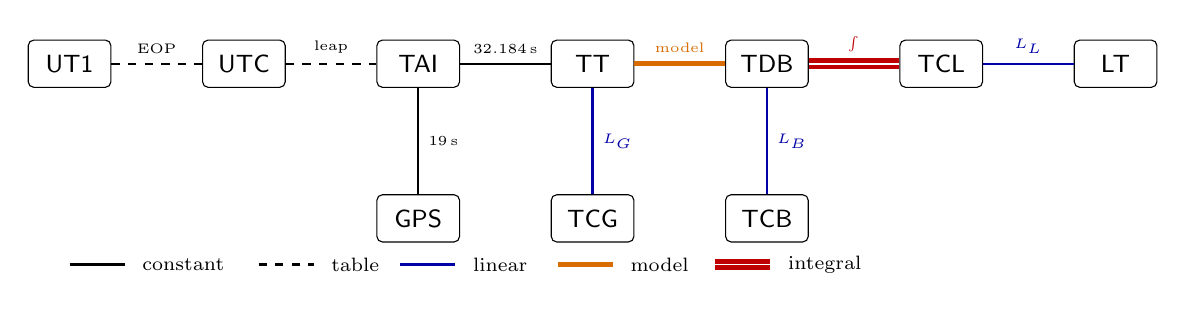
\begin{tikzpicture}[node distance=1.35cm and 1.15cm]
    \node[tsnode] (ut1) {UT1};
    \node[tsnode, right=of ut1] (utc) {UTC};
    \node[tsnode, right=of utc] (tai) {TAI};
    \node[tsnode, right=of tai] (tt)  {TT};
    \node[tsnode, right=of tt]  (tdb) {TDB};
    \node[tsnode, right=of tdb] (tcl) {TCL};
    \node[tsnode, right=of tcl] (lt)  {LT};
    \node[tsnode, below=of tai] (gps) {GPS};
    \node[tsnode, below=of tt]  (tcg) {TCG};
    \node[tsnode, below=of tdb] (tcb) {TCB};

    \draw[table]    (ut1) -- node[above, font=\tiny] {EOP}  (utc);
    \draw[table]    (utc) -- node[above, font=\tiny] {leap} (tai);
    \draw[constant] (tai) -- node[above, font=\tiny] {\SI{32.184}{\second}} (tt);
    \draw[model]    (tt)  -- node[above, font=\tiny] {model} (tdb);
    \draw[integral] (tdb) -- node[above, font=\tiny] {$\int$} (tcl);
    \draw[linear]   (tcl) -- node[above, font=\tiny] {$L_L$} (lt);
    \draw[constant] (tai) -- node[right, font=\tiny] {\SI{19}{\second}} (gps);
    \draw[linear]   (tt)  -- node[right, font=\tiny] {$L_G$} (tcg);
    \draw[linear]   (tdb) -- node[right, font=\tiny] {$L_B$} (tcb);

    \begin{scope}[shift={(0,-2.55)}, every node/.style={font=\scriptsize, anchor=west}]
      \draw[constant] (0,0)   -- (0.7,0);   \node at (0.8,0)   {constant};
      \draw[table]    (2.4,0) -- (3.1,0);   \node at (3.2,0)   {table};
      \draw[linear]   (4.2,0) -- (4.9,0);   \node at (5.0,0)   {linear};
      \draw[model]    (6.2,0) -- (6.9,0);   \node at (7.0,0)   {model};
      \draw[integral] (8.2,0) -- (8.9,0);   \node at (9.0,0)   {integral};
    \end{scope}
  \end{tikzpicture}
  \caption{The registered conversion graph. Every edge returns an
  \emph{offset}; a conversion is the sum of the offsets along the shortest
  route. Edge classes are ordered by cost: constant and table edges are
  arithmetic or a lookup, linear edges rescale elapsed time by
  $L\sim10^{-8}$, the TT\,$\leftrightarrow$\,TDB edge evaluates the active
  model, and the TDB\,$\leftrightarrow$\,TCL edge integrates from $T_0$. The
  graph is drawn undirected only for legibility: each edge is registered in
  both directions, with the inverse offset.}
  \label{fig:tc-graph}
\end{figure}

\begin{table}[htbp]
  \centering
  \caption{Edge classes and their cost. The spread is why the route matters.}
  \label{tab:tc-edges}
  \begin{tabularx}{\textwidth}{llL}
    \toprule
    Class & Edges & Cost \\
    \midrule
    constant & TAI\,$\leftrightarrow$\,TT, TAI\,$\leftrightarrow$\,GPS & arithmetic \\
    table    & TAI\,$\leftrightarrow$\,UTC (leap seconds),
               UTC\,$\leftrightarrow$\,UT1 (EOP) & table lookup \\
    linear   & TT\,$\leftrightarrow$\,TCG, TDB\,$\leftrightarrow$\,TCB,
               TCL\,$\leftrightarrow$\,LT & rescaling of elapsed time by $L\sim10^{-8}$ \\
    model    & TT\,$\leftrightarrow$\,TDB & Chebyshev fit, DE440 integral, or analytic series \\
    integral & TDB\,$\leftrightarrow$\,TCL & trapezoidal sweep from $T_0$ (1977) \\
    \bottomrule
  \end{tabularx}
\end{table}

TCL\,$\leftrightarrow$\,LT and TDB\,$\leftrightarrow$\,TCB are single linear
edges and are reached without touching the TDB\,$\leftrightarrow$\,TCL
integral. The search minimises hops, which coincides with minimum cost for
this edge set because the one expensive edge is also the only bridge to the
lunicentric scales: no route can avoid it that needs it, and no route incurs it
that does not. Adding an edge that breaks that coincidence would require a
cost-weighted search.

\begin{lstlisting}[language=cpp,caption={The registered edge table, abridged.},label={lst:tc-edges}]
// cpp/lupnt/conversions/epoch.cc :: TimeEdges
const std::map<std::pair<Time, Time>, TimeOffsetFn>& TimeEdges() {
  static const std::map<std::pair<Time, Time>, TimeOffsetFn> edges = {
      // --- constant offsets ---
      {{Time::TAI, Time::TT},  [](Real) { return Real(TT_TAI_OFFSET); }},
      {{Time::TAI, Time::GPS}, [](Real) { return Real(-19.0); }},

      // --- leap seconds / Earth orientation ---
      {{Time::TAI, Time::UTC},
       [](Real t_tai) { return Real(-GetTaiUtcDifference(TimeToMjd(t_tai).val())); }},
      {{Time::UTC, Time::UT1},
       [](Real t_utc) { return GetUt1UtcDifference(TimeToMjd(t_utc)); }},

      // --- linear rescalings (elapsed time only ever scaled by L ~ 1e-8) ---
      {{Time::TT,  Time::TCG},
       [](Real t_tt)  { return L_G / (1.0 - L_G) * (t_tt - T0Seconds()); }},
      {{Time::TDB, Time::TCB},
       [](Real t_tdb) { return (L_B * (t_tdb - T0Seconds()) - TDB_0) / (1.0 - L_B); }},
      {{Time::TCL, Time::LT},
       [](Real t_tcl) { return -L_L * (t_tcl - T0Seconds()); }},

      // --- the two model edges ---
      {{Time::TDB, Time::TT},  [](Real t_tdb) { return TtMinusTdb(t_tdb); }},
      {{Time::TDB, Time::TCL}, [](Real t_tdb) { return -TdbMinusTcl(t_tdb); }},
      // ... every edge is also registered in the reverse direction ...
  };
  return edges;
}
\end{lstlisting}

\subsection{Offset accessors}
\label{sec:tc-offset-accessors}

An interface that must \emph{return} an absolute epoch cannot benefit from
\cref{eq:tc-compose}; it is capped near the ULP however good the underlying
model is. \Cref{tab:tc-entrypoints} states the resulting contract.

\begin{table}[htbp]
  \centering
  \caption{What each entry point returns, and the accuracy that follows from
  the return type. Measured for TDB\,$\leftrightarrow$\,TT over 2020--2035.}
  \label{tab:tc-entrypoints}
  \begin{tabularx}{\textwidth}{lLl}
    \toprule
    Entry point & Returns & Accuracy \\
    \midrule
    \cpp{Epoch::To} / \cpp{TimeScaleOffset} & offset & \SI{4e-4}{\nano\second} \\
    \cpp{TtMinusTdb}, \cpp{TdbMinusTcl}, \cpp{TdbMinusLt} & offset & \SI{4e-4}{\nano\second} \\
    \cpp{ConvertTime} & absolute epoch & \SI{38}{\nano\second} rms, \SI{119}{\nano\second} peak \\
    \bottomrule
  \end{tabularx}
\end{table}

\cpp{ConvertTime(t, from, to)} delegates to \cpp{Epoch}; its floor is a
property of the return type, not of the model.

\begin{lstlisting}[language=py,caption={Choosing an interface in Python.},label={lst:tc-python}]
import pylupnt as pnt

e     = pnt.Epoch.from_seconds(t_tai, pnt.Time.TAI)
e_tdb = e.to(pnt.Time.TDB)                        # offset-composing, exact
dt    = pnt.time_scale_offset(e, pnt.Time.TCL)    # offset, sub-picosecond

t_tt  = pnt.convert_time(t_tai, pnt.Time.TAI, pnt.Time.TT)   # ~245 ns floor
\end{lstlisting}

\section{Proper versus coordinate time}
\label{sec:tc-proper-coordinate}

A clock measures \textbf{proper time} $\tau$ along its worldline, while a
\textbf{coordinate time} $t$ labels events in a four-dimensional relativistic
reference system (BCRS, GCRS, LCRS) and cannot be read off any single physical
clock \citep[Ch.~2.3.1]{iiyama2026thesis}. \cpp{IsCoordinateTimeScale}
partitions the enum: TT, TCG, TDB, TCB, TCL, and LT are coordinate scales;
UT1, UTC, TAI, and GPS are not.

\begin{lstlisting}[language=cpp]
// cpp/lupnt/conversions/time_conversions.cc :: IsCoordinateTimeScale
case Time::TT: case Time::TCG: case Time::TDB:
case Time::TCB: case Time::TCL: case Time::LT: return true;
\end{lstlisting}

\cpp{ConvertCoordinateTime} is the coordinate-only entry point. Its
position-aware overloads take a BCRS position $\vec{x}_{\mathrm{bcrs}}$ so that
the position-dependent terms of the TDB/TCB/TCL transforms are evaluated at the
event location rather than at the body centre.

\section{Atomic and terrestrial scales}
\label{sec:tc-atomic}

\paragraph{TAI to TT} is a defining constant offset
\citep[Eq.~2.38]{iiyama2026thesis}:
%
\begin{equation}
\label{eq:tc-tai-tt}
  \TT = \TAI + \SI{32.184}{\second} .
\end{equation}

\begin{lstlisting}[language=cpp]
// cpp/lupnt/conversions/time_conversions.cc :: TaiToTt / TtToTai
Real TaiToTt(Real t_tai) { return t_tai + TT_TAI_OFFSET; }   // TT_TAI_OFFSET = 32.184 s
Real TtToTai(Real t_tt)  { return t_tt  - TT_TAI_OFFSET; }
\end{lstlisting}

\paragraph{TAI to GPS} is the fixed \SI{19}{\second} offset that removes the
leap seconds accumulated at the GPS epoch
\citep[Eq.~2.39]{iiyama2026thesis}; GPS time runs without leap seconds
thereafter:
%
\begin{equation}
\label{eq:tc-gps}
  \GPST = \TAI - \SI{19}{\second} .
\end{equation}

\begin{lupntnote}
Only GPS is implemented among the GNSS scales. The thesis also lists
GLONASS $= \TAI - \SI{34}{\second}$ (leap-tracking, offset by UTC),
Galileo $= \TAI - \SI{19}{\second}$, and BeiDou $= \TAI - \SI{33}{\second}$
(Eqs.~2.40--2.42); these are not in the \code{Time} enum.
\end{lupntnote}

\paragraph{TAI and UTC} differ by the integer leap-second table
$\Delta_{\mathrm{AT}}(\mathrm{MJD})$ from \file{cpp/lupnt/interfaces/tai_utc.h}
\citep[Eq.~2.43]{iiyama2026thesis}:
%
\begin{equation}
\label{eq:tc-utc}
  \UTC = \TAI - \Delta_{\mathrm{AT}},
  \qquad
  \Delta_{\mathrm{AT}} = \cpp{GetTaiUtcDifference}(\mathrm{MJD}) .
\end{equation}

\paragraph{UTC and UT1} differ by the observed Earth-orientation correction
looked up from the EOP table (\file{cpp/lupnt/interfaces/eop.h}):
%
\begin{equation}
\label{eq:tc-ut1}
  \UTone = \UTC + (\UTone - \UTC),
  \qquad
  (\UTone - \UTC) = \cpp{GetUt1UtcDifference}(\mathrm{MJD}) .
\end{equation}

\begin{lstlisting}[language=cpp]
// cpp/lupnt/conversions/time_conversions.cc :: UtcToUt1
Real mjd_utc = t_utc / SECS_DAY + MJD_J2000_TT;
Real ut1_utc = GetUt1UtcDifference(mjd_utc);
return t_utc + ut1_utc;
\end{lstlisting}

UT1 in turn drives Earth rotation. \cpp{EarthRotationAngle} gives the ERA
%
\begin{equation}
\label{eq:tc-era}
  \theta = 2\pi\left(0.7790572732640
           + 1.00273781191135448\,\frac{t_{\UTone}}{86400}\right),
\end{equation}
%
and \cpp{GreenwichMeanSiderealTime} / \cpp{GreenwichApparentSiderealTime} give
GMST and GAST, the latter adding the equation of the equinoxes. These are the
only rotation quantities keyed on UT1; see \cref{chap:frame-conversions}.

\section{Barycentric and geocentric coordinate scales}
\label{sec:tc-bary}

The four Einstein-scaled coordinate times share the reference epoch
$T_0 = $ 1977-01-01 00:00:00 TAI (\code{MJD\_COORDINATE\_TT\_TCG\_TCB}) and the
defining rates \citep{iers2010}
%
\begin{equation}
\label{eq:tc-rates}
  L_B = 1.550519768\times10^{-8},\quad
  L_G = 6.969290134\times10^{-10},\quad
  \TDB_0 = \SI{-65.5}{\micro\second} .
\end{equation}
%
Writing $\tau = t - T_0$ for elapsed time from the coordinate-time origin, the
constant and linear edges of \cref{fig:tc-graph} are
%
\begin{align}
  \label{eq:tc-linear}
  \TCG - \TT   &= \frac{L_G}{1 - L_G}\,\tau_{\TT}, &
  \TCB - \TDB  &= \frac{L_B\,\tau_{\TDB} - \TDB_0}{1 - L_B}, \\
  \LT - \TCL   &= -L_L\,\tau_{\TCL}, &
  \UTC - \TAI  &= -\Delta_{\mathrm{AT}}(t) .
\end{align}

\begin{lstlisting}[language=cpp]
// cpp/lupnt/conversions/time_conversions.cc :: TtToTcg  (offset form)
Real tt_tcg = -L_G / (1.0 - L_G) * (mjd_tt - MJD_COORDINATE_TT_TCG_TCB) * SECS_DAY;
return t_tt - tt_tcg;

// cpp/lupnt/conversions/time_conversions.cc :: TcbToTdb
Real t_tdb = t_tcb - L_B * (mjd_tcb - MJD_COORDINATE_TT_TCG_TCB) * SECS_DAY + TDB_0;
\end{lstlisting}

Only the two remaining edges, TT\,$\leftrightarrow$\,TDB and
TDB\,$\leftrightarrow$\,TCL, require a relativistic model.

\section{The TT--TDB model}
\label{sec:tc-tttdb}

\subsection{The DE440 relation}

The barycentric edge is the DE440 relativistic relation
\citep[Eqs.~3--7]{park2021de440}. With $s_B = (1-L_G)/(1-L_B)$ and a station at
BCRS position $\vec{r}_S$,
%
\begin{equation}
\label{eq:tc-de440}
\begin{aligned}
  \TDB - \TT
    &= \frac{L_G - L_B}{1 - L_B}\,\tau_{\TDB}
     + s_B\,\TDB_0
     + \frac{s_B}{c^{2}} \int_{T_0 + \TDB_0}^{\TDB} f_2 \,\dd t
     - \frac{s_B}{c^{4}} \int_{T_0 + \TDB_0}^{\TDB} f_4 \,\dd t \\[2pt]
    &\quad + \frac{1}{c^{2}}\,\vec{v}_E \cdot (\vec{r}_S - \vec{r}_E)
     + \frac{1}{c^{4}}\left(3 w_{0E} + \tfrac{1}{2} v_E^{2}\right)
       \vec{v}_E \cdot (\vec{r}_S - \vec{r}_E),
\end{aligned}
\end{equation}
%
where the integrands collect the Earth's kinetic and potential terms,
%
\begin{align}
  \label{eq:tc-f2}
  f_2 &= \tfrac{1}{2} v_E^{2} + w_{0E} + w_{LE}, \\
  \label{eq:tc-f4}
  f_4 &= -\tfrac{1}{8} v_E^{4} - \tfrac{3}{2} v_E^{2} w_{0E}
         + 4\,\vec{v}_E \cdot \vec{w}_{iE}
         + \tfrac{1}{2} w_{0E}^{2} + \Delta_E ,
\end{align}
%
and $w_{0E}$ is the external potential at the Earth,
%
\begin{equation}
\label{eq:tc-w0e}
  w_{0E} = \sum_{i \neq E} \frac{GM_i}{r_{iE}}
  + U_{\mathrm{ring}}(r_{\odot E};\, GM_{\mathrm{ast}}, a_{\mathrm{ast}})
  + U_{\mathrm{ring}}(r_{\odot E};\, GM_{\mathrm{KB}}, a_{\mathrm{KB}}),
\end{equation}
%
with $w_{LE}$ the solar oblateness potential, $\vec{w}_{iE}$ the mass-weighted
velocity potential, and $\Delta_E$ the remaining $c^{-4}$ terms. The two ring
terms are \cref{sec:tc-smallbody}. At the geocentre $\vec{r}_S = \vec{r}_E$ and
both endpoint terms vanish, leaving only the integrals.

\subsection{The model chain}
\label{sec:tc-model-chain}

Evaluating \cref{eq:tc-de440} means sweeping from $T_0$, so it is not viable
per call. \cpp{TtMinusTdb(t)} is the single implementation of the TT--TDB
relation --- both \cpp{TtToTdb} and \cpp{TDBToTt} delegate to it, so the pair
round-trips exactly whichever model is active --- and it selects, in order:

\begin{enumerate}[leftmargin=*]
  \item \textbf{Chebyshev fit of the DE440t TT--TDB ephemeris.}
    \cpp{InitTtMinusTdbFit} samples the \file{de440t.bsp} time-ephemeris
    segment as a clean offset and fits piecewise Chebyshev segments (16-day
    segments, degree 12). Reproduces the kernel to \SI{4e-4}{\nano\second}.
  \item \textbf{DE440 integral}, \cref{eq:tc-de440}, opt-in via
    \cpp{SetTtTdbModel(TtTdbModel::DE440\_INTEGRAL)}. Trapezoidal sweep of the
    $c^{-2}$ and $c^{-4}$ integrands from $T_0$; agrees with the DE440t
    ephemeris to \SI{2.4}{\nano\second} rms with a residual secular term
    (\cref{sec:tc-boundaries}).
  \item \textbf{Auto-fit}: if no fit covers the requested epoch, one
    decade-wide window is built on demand (\cpp{SetTtTdbAutoFit}, default on).
    This is what makes the \emph{default} accuracy \SI{4e-4}{\nano\second} for
    every caller --- \cpp{ConvertTime}, \cpp{Epoch}, and the offset accessors
    alike.
  \item \textbf{Analytic fallback}, used only when the DE440t segment is
    unavailable: the two-term IAU/IERS series \citep{urban2013},
    %
    \begin{equation}
    \label{eq:tc-series}
      \TDB - \TT \approx
      \SI{0.001658}{\second}\,\sin g + \SI{0.000014}{\second}\,\sin 2g,
    \end{equation}
    %
    with $g = \ang{357.53} + \ang{0.9856003}\,d_{\mathrm{J2000}}$ the Earth's
    mean anomaly, good to $\lesssim\SI{2}{\milli\second}$.
\end{enumerate}

\begin{lupntnote}
The \textbf{position-aware} overloads \cpp{TtToTdb(t, x\_bcrs)} and
\cpp{TDBToTt(t, x\_bcrs)} evaluate the full GCRS\,$\leftrightarrow$\,BCRS
four-dimensional transform \citep[Eqs.~21--22]{turyshev2026cislunar}: a
trapezoidal integral of the $c^{-2}$ and $c^{-4}$ integrands built from the
Earth's barycentric velocity and the external Solar-System potential
$w_{\mathrm{ext}} = \sum_{B \neq E} GM_B / r_{EB}$, plus a position term
$-\vec{v}_E \cdot \vec{r}_E / c^2$. \cpp{TtToTdb(t, x\_bcrs)} inverts by
10-step Newton iteration.
\end{lupntnote}

\subsection{Small-body populations}
\label{sec:tc-smallbody}

DE440 integrates the solar system with 343 discrete asteroids, 30 individual
Kuiper-belt objects, and a 36-point circular ring representing the rest of the
Kuiper belt at \SI{44}{\au} \citep{park2021de440}. \lupnt{} carries no
ephemerides for any of them. Omitting that mass leaves a near-constant deficit
in the external potential, which \cref{eq:tc-de440} integrates into a purely
secular drift.

Each population is therefore added as a uniform circular ring of mass $M$ and
radius $a$, whose potential at heliocentric distance $r$ in the ring plane is
%
\begin{equation}
\label{eq:tc-ring}
  U(r) = \frac{2GM}{\pi(a+r)}\,K(k),
  \qquad k = \frac{2\sqrt{ar}}{a+r} .
\end{equation}
%
It is evaluated at the body's actual heliocentric distance at each step, so it
carries the small annual modulation rather than being held constant.

The factor $K$ is the complete elliptic integral of the first kind
\citep[Ch.~17]{abramowitz1964},
%
\begin{equation}
\label{eq:tc-elliptic}
  K(k) = \int_{0}^{\pi/2} \frac{\dd\theta}{\sqrt{1 - k^{2}\sin^{2}\theta}} .
\end{equation}
%
It arises for a geometric reason: the potential of a ring is the sum of $GM/d$
over every element of it, and the distance $d$ from the field point to a ring
element varies around the ring; integrating $1/d$ over the ring angle produces
exactly \cref{eq:tc-elliptic}. The modulus $k \in [0,1)$ measures how close the
field point is to the ring. As $k \to 0$ (far away) $K \to \pi/2$ and
\cref{eq:tc-ring} reduces to the point-mass potential $GM/r$; as $k \to 1$ (on
the ring) $K$ diverges logarithmically. For the Earth inside a \SI{44}{\au}
ring, $k$ is small and the ring is a mild correction to a point mass --- but a
correction with the right radial dependence, which is what the secular drift is
sensitive to.

\lupnt{} evaluates \cref{eq:tc-elliptic} by the arithmetic--geometric mean
(AGM) \citep[\S17.6]{abramowitz1964}: iterating
$a_{n+1} = \tfrac{1}{2}(a_n + b_n)$, $b_{n+1} = \sqrt{a_n b_n}$ from $a_0 = 1$,
$b_0 = \sqrt{1-k^{2}}$ converges quadratically to a common limit $M(k)$, and
$K(k) = \pi / \bigl(2 M(k)\bigr)$.

\begin{lstlisting}[language=cpp,caption={The ring potential, built from arithmetic and square roots so that it composes with automatic differentiation.},label={lst:tc-ring}]
// cpp/lupnt/conversions/time_conversions.cc :: RingPotential
// k' = sqrt(1-k^2). AGM converges quadratically (~5 iterations here) and is
// differentiable, so this composes with autodiff unlike std::comp_ellint_1.
Real RingPotential(Real r, double gm_ring, double a_ring) {
  if (gm_ring == 0.0) return Real(0.0);
  Real apr = a_ring + r;
  Real k2  = 4.0 * a_ring * r / (apr * apr);
  Real a = 1.0;
  Real b = sqrt(1.0 - k2);            // complementary modulus k'
  for (int i = 0; i < 12; i++) {
    Real a_next = 0.5 * (a + b);
    b = sqrt(a * b);
    a = a_next;
    if (abs((a - b).val()) < 1e-16) break;
  }
  Real K = PI / (2.0 * a);
  return 2.0 * gm_ring * K / (PI * apr);
}
\end{lstlisting}

\begin{table}[htbp]
  \centering
  \caption{Ring parameters, taken from DE440's own integration header rather
  than from independently published values. See the caveat below.}
  \label{tab:tc-rings}
  \begin{tabular}{lrr}
    \toprule
    Population & $GM$ [\si{\meter\cubed\per\second\squared}] & Ring radius [\si{\au}] \\
    \midrule
    Kuiper ring $+$ 30 KBOs & $1.1232\times10^{13}$ & 44 \\
    343 asteroids           & $1.7053\times10^{11}$ & 2.7 \\
    \bottomrule
  \end{tabular}
\end{table}

\begin{lupntwarning}
DE440 \emph{fitted} its ring mass during the integration, so
\cref{tab:tc-rings} is not the published Kuiper-belt total --- the
independently derived value is smaller by a factor of $1.43$. Only the value
DE440 actually integrated reproduces its TT--TDB. These are therefore
reproduction constants, not physical mass estimates: they should not be reused
as measurements of either population, nor tuned against any residual. For
sub-nanosecond absolute agreement with JPL use the Chebyshev fit instead.
\end{lupntwarning}

\section{Lunicentric coordinate scales}
\label{sec:tc-lunar}

The Moon's analogues follow \citet{turyshev2026cislunar}, with LCRS as the
lunar four-dimensional system. Reaching lunar time uses the same construction
one level down, with the Moon in place of the Earth.

\subsection{TCB to TCL}

TCL is the coordinate time of the Lunicentric Celestial Reference System. The
barycentric-to-lunicentric transform \citep[Eqs.~23,~25]{turyshev2026cislunar},
\citep[Eqs.~2.44--2.45]{iiyama2026thesis} is structurally identical to the
Earth case with the Moon substituted:
%
\begin{equation}
\label{eq:tc-tcbtcl}
  \TCL = \TCB
    - \frac{1}{c^2}\!\int\!\Bigl(\tfrac{1}{2}v_M^2 + w_{\mathrm{ext}}(\vec{x}_M)\Bigr)\dd\TCB
    - \frac{1}{c^4}\!\int (\cdots)\,\dd\TCB
    - \frac{\vec{v}_M \cdot \vec{r}_M}{c^2} - \cdots
\end{equation}
%
where $\vec{r}_M = \vec{x}_{\mathrm{bcrs}} - \vec{x}_M$,
$\vec{v}_M = \dd\vec{x}_M/\dd\TCB$, and
$w_{\mathrm{ext}}(\vec{x}_M) = \sum_{B \neq M} GM_B / |\vec{x}_M - \vec{x}_B|$
sums the Sun, Mercury, Venus, Earth, Mars, and the outer planets
(\code{kTclExternalBodies}), plus the same two rings of
\cref{sec:tc-smallbody}. Passing no position places the clock at the lunar
centre ($\vec{v}_M \cdot \vec{r}_M = 0$). \cpp{TclToTcb} inverts by Newton
iteration.

Equivalently, in the offset form the graph edge uses,
%
\begin{equation}
\label{eq:tc-tcl}
  \TDB - \TCL
   = -L_B\,\tau_{\TCB} + \TDB_0
   + \frac{1}{c^{2}} \int_{T_0}^{\TCB} g_2 \,\dd t
   + \frac{1}{c^{4}} \int_{T_0}^{\TCB} g_4 \,\dd t,
\end{equation}
%
\begin{equation}
\label{eq:tc-g24}
  g_2 = \tfrac{1}{2} v_M^{2} + w_{0M},
  \qquad
  g_4 = \tfrac{1}{8} v_M^{4} + \tfrac{3}{2} v_M^{2} w_{0M} - \tfrac{1}{2} w_{0M}^{2},
\end{equation}
%
where $w_{0M}$ is \cref{eq:tc-w0e} evaluated at the Moon.

\begin{lstlisting}[language=cpp]
// cpp/lupnt/conversions/time_conversions.cc :: TcbToTcl  (Turyshev Eq. 23/25)
auto [i2, i4] = IntegrateTcbToTclTerms(t_tcb);
return t_tcb - i2/(C*C) - i4/(C*C*C*C) + TcbToTclPositionTerm(t_tcb, x_bcrs);
\end{lstlisting}

\subsection{TCL to LT}

LT is the lunar analogue of TT: a defining rate on the selenoid
\citep[Eqs.~2.48--2.49]{iiyama2026thesis} with
$L_L = 3.139054\times10^{-11}$,
%
\begin{equation}
\label{eq:tc-lt}
  \LT = \TCL - L_L\,(\TCL - T_{L0}),
  \qquad
  \frac{\dd \LT}{\dd \TCL} = 1 - L_L .
\end{equation}

\begin{lstlisting}[language=cpp]
// cpp/lupnt/conversions/time_conversions.cc :: TclToLt  (T_L0 assumed = T_0)
Real lt_tcl = -L_L * (mjd_tcl - MJD_COORDINATE_TT_TCG_TCB) * SECS_DAY;
return t_tcl + lt_tcl;
\end{lstlisting}

\begin{lupntwarning}
$L_L$ is not yet internationally standardized. The code uses the Turyshev
selenoid value $3.139054\times10^{-11}$ (potential
$\Phi_L = 2.82123744381\times10^{6}\ \si{\meter\squared\per\second\squared}$),
whereas \citet{kopeikin2024lunar} adopt $3.14027\times10^{-11}$
\citep[Ch.~2.3.5]{iiyama2026thesis}. LT is therefore provisional pending
standardization.
\end{lupntwarning}

\subsection{Lunar time as a function of TT: the direct path}
\label{sec:tc-lt-direct}

Rather than chaining TT\,$\to$\,TDB\,$\to$\,TCB\,$\to$\,TCL\,$\to$\,LT,
\lupnt{} also implements LT directly as an Earth--Moon \emph{difference}
\citep[Eq.~57]{turyshev2026cislunar}, the TDB-argument form of thesis
Eq.~2.50, in \cpp{TdbToLtMinusTt}:
%
\begin{equation}
\label{eq:tc-ltmtt}
\begin{aligned}
  \LT - \TT
    &= \frac{L_G - L_L}{1 - L_B}\left(\TDB - T_0 - \TDB_0\right) \\[2pt]
    &\quad - \frac{1}{c^{2}} \int_{T_0 + \TDB_0}^{\TDB}
       \left[ \tfrac{1}{2} v_{EM}^{2}
            + \frac{GM_E - 2\,GM_M}{r_{EM}}
            + W^{\odot}_{EM}
            + \tfrac{3}{2} L_G \frac{GM_S}{r_{SE}} \right] \dd t \\[2pt]
    &\quad + \frac{1}{c^{2}}
       \Bigl[ \vec{v}_E \cdot \vec{r}_{EM} \Bigr]_{\TDB}^{T_0 + \TDB_0}
     - \frac{3}{c^{4}} \int_{T_0 + \TDB_0}^{\TDB}
       \frac{GM_S}{r_{SE}}\, \vec{v}_E \cdot \vec{v}_{EM} \,\dd t,
\end{aligned}
\end{equation}
%
with the solar $\ell = 2$ tidal term
%
\begin{equation}
\label{eq:tc-tidal}
  W^{\odot}_{EM} = \frac{3}{2}\,\frac{GM_S}{r_{SE}^{5}}
    \left[ (\vec{r}_{ES} \cdot \vec{r}_{EM})^{2}
         - \tfrac{1}{3} r_{SE}^{2} r_{EM}^{2} \right].
\end{equation}

\begin{lupntnote}
The factor of two on $GM_M$ in \cref{eq:tc-ltmtt} is not a typo: one $-GM_M$
comes from TCL\,--\,TCG, and a second from the $L_L$ rescaling that defines LT.
Because \cref{eq:tc-ltmtt} contains only Earth--Moon differences, distant
bodies --- including the small-body rings of \cref{sec:tc-smallbody} ---
cancel identically and are deliberately omitted from it. Including them there
would add ${\sim}10^{-9}\ \si{\meter\squared\per\second\squared}$ of numerical
noise rather than physics.
\end{lupntnote}

The integral is a trapezoidal sweep at $\dd t = \SI{0.01}{\dayunit}$. For
repeated queries in a window, \cpp{InitLtMinusTtFit} fits piecewise Chebyshev
segments (degree 12, 1-day segments) over the window in a single forward sweep
and caches them; \cpp{TdbToLtMinusTt} then uses the fast path
(\cpp{ChebyshevFitModel::Eval}, \file{cpp/lupnt/numerics/cheby_fit.h}).

\begin{lstlisting}[language=cpp]
// cpp/lupnt/conversions/time_conversions.cc :: TdbToLt / TtToLt
Real TdbToLt(Real t_tdb) { return TDBToTt(t_tdb) + TdbToLtMinusTt(t_tdb); }
Real TtToLt(Real t_tt)   { return TdbToLt(TtToTdb(t_tt)); }
\end{lstlisting}

\cpp{LtToTdb} and \cpp{LtToTt} invert by 10-step Newton iteration. That
\lupnt{} reaches LT by two genuinely different formulations --- the absolute
lunar potential of \cref{eq:tc-tcl} and the Earth--Moon difference of
\cref{eq:tc-ltmtt} --- makes their agreement a real check rather than a
tautology.

A separate lunar-surface proper-time term is provided by
\cpp{GetProperTimeCorrectionTcl(t\_tcg, x\_mci)}, the first-order clock
correction $-\vec{v}_{LE}\cdot(\vec{r}_x - \vec{r}_{LE})/c^2$ for a clock at
MCI position $\vec{x}_{\mathrm{mci}}$ relative to the Moon's geocentric motion.

\section{Exact calendar input}
\label{sec:tc-calendar}

The chain from a calendar date to an epoch is a second place where precision
can be lost before any conversion happens. Routing through a Modified Julian
Date rounds at the coarsest point in the chain: MJD counts days from 1858, so
one ULP of an MJD at present-day epochs is \SI{1129}{\nano\second} --- eight
times coarser than seconds-from-J2000, because its origin sits eight times
further away. Whole minutes survive that (their fraction-of-day is a dyadic
rational) but arbitrary clock times do not.

\cpp{Epoch::FromGregorian} therefore computes the integer second with integer
arithmetic \citep{hinnant2013} and carries only the sub-second remainder as a
floating-point value:

\begin{lstlisting}[language=cpp,caption={Integer-exact calendar conversion.},label={lst:tc-fromgregorian}]
// cpp/lupnt/conversions/epoch.cc :: Epoch::FromGregorian
const int64_t days = DaysFromCivil(year, month, day) - kDaysCivilToJ2000;
const double  s       = sec.val();
const double  s_floor = std::floor(s);
const int64_t whole   = days * 86400 + static_cast<int64_t>(hour) * 3600
                        + static_cast<int64_t>(min) * 60
                        + static_cast<int64_t>(s_floor) - kJ2000NoonOffset;
return Epoch(whole, sec - s_floor, scale);
\end{lstlisting}

The measured input error across a set of calendar dates including non-dyadic
clock times is \SI{0.0}{\nano\second}, against \SI{358}{\nano\second} for the
MJD-routed path. Dates before the Gregorian reform
defer to the MJD path, which handles the calendar discontinuity.

\section{Conversion of physical quantities and constants}
\label{sec:tc-scaling}

Because the scaled coordinate times (TT, TDB, LT) run at rates $(1-L_G)$,
$(1-L_B)$, $(1-L_L)$ relative to their unscaled partners (TCG, TCB, TCL),
spatial coordinates and gravitational parameters must be rescaled to keep $c$
and the equations of motion invariant
\citep[Eqs.~2.52--2.57]{iiyama2026thesis}:
%
\begin{align}
  \label{eq:tc-scale-tt}
  \mathcal{X}_{\TT}  &= (1-L_G)\,\mathcal{X}_{\TCG}, &
  \mu_{\TT}          &= (1-L_G)\,\mu_{\TCG}, \\
  \label{eq:tc-scale-tdb}
  \mathcal{X}_{\TDB} &= (1-L_B)\,\mathcal{X}_{\TCB}, &
  \mathcal{X}_{\LT}  &= (1-L_L)\,\mathcal{X}_{\TCL}.
\end{align}
%
\lupnt{} encodes these as the \code{CoordinateScale} factors $1 - L_x$, with
\cpp{CoordinateScaleRatio(from, to)} returning
$(1-L_{\mathrm{to}})/(1-L_{\mathrm{from}})$ for the rescale, guarded by
\cpp{AreCoordinateScalesConvertible} --- only
barycentric\,$\leftrightarrow$\,barycentric,
geocentric\,$\leftrightarrow$\,geocentric, and
lunicentric\,$\leftrightarrow$\,lunicentric pairs share a constant factor.

\begin{lstlisting}[language=cpp]
// cpp/lupnt/core/constants.h :: CoordinateScaleFactor
case CoordinateScale::TDB: return 1.0 - L_B;
case CoordinateScale::TT:  return 1.0 - L_G;
case CoordinateScale::TL:  return 1.0 - L_L;
\end{lstlisting}

\section{Model boundaries}
\label{sec:tc-boundaries}

\begin{itemize}[leftmargin=*]
  \item All API times are seconds from the per-scale J2000 origin; calendar
    input and output go through \cpp{GregorianToTime} /
    \cpp{TimeToGregorianString}, or --- preferably ---
    \cpp{Epoch::FromGregorian} (\cref{sec:tc-calendar}).
  \item Only GPS is implemented among the GNSS scales; GLONASS, Galileo, and
    BeiDou offsets are documented but not exposed.
  \item \cpp{ConvertTime} and \cpp{ConvertCoordinateTime} return absolute
    epochs and are therefore bounded near \SI{245}{\nano\second} regardless of
    model quality. Use \cpp{Epoch} or the offset accessors below that level.
  \item The DE440 integral of \cref{eq:tc-de440} carries a small secular
    difference against the DE440t ephemeris, dominated by the ring
    approximation of \cref{sec:tc-smallbody}. Refining the trapezoidal step
    from \SI{864}{\second} to \SI{216}{\second} moves the drift by
    \SI{0.0005}{\nano\second\per\yr}, so the residual is a model difference
    and not quadrature. Use the Chebyshev fit when absolute agreement with JPL
    matters.
  \item \cpp{TdbMinusTcl} and \cpp{TdbToLtMinusTt} integrate from $T_0$ per
    call. Both auto-fit a decade-wide Chebyshev window on demand
    (\cpp{SetTdbTclAutoFit}, \cpp{InitLtMinusTtFit}); with auto-fitting
    disabled a single lunar conversion costs seconds.
  \item $L_L$, and hence LT, is provisional pending international
    standardization.
\end{itemize}

\chapter{Reference Frames and Frame Conversions}
\label{chap:frame-conversions}

This chapter specifies every reference frame \lupnt{} knows about, the exact
rotation and translation that relates each adjacent pair, the time scale each
rotation is evaluated in, and the velocity transformation that accompanies
each rotation. The public dispatch --- \cpp{ConvertFrame},
\cpp{GetFrameRotationTranslation}, \cpp{GetFrameRotationTranslationRv} and
\cpp{GetFrameCenter} --- is implemented in
\file{cpp/lupnt/conversions/frame_converter.cc} and declared in
\file{cpp/lupnt/conversions/frame_converter.h}, which also owns the
\cpp{Frame} enumeration. The individual body-pair rotations
(\cpp{GcrfToItrf}, \cpp{GcrfToMoonCi}, \cpp{RotMoonCiToPa}, the IAU planet
orientation, \dots) live in
\file{cpp/lupnt/conversions/frame_conversions.cc} and
\file{cpp/lupnt/conversions/frame_conversions.h}. The topocentric
(east--north--up, azimuth--elevation--range) helpers are in
\file{cpp/lupnt/conversions/coordinate_conversions.cc}.

The Earth models follow the IAU 2006/2000A conventions of
\citep{iers2010}, with the classical background of \citep{montenbruck2000}
and \citep{vallado2013}. The Earth--Moon translation and the lunar mantle
libration angles come from the JPL DE440 ephemeris \citep{park2021de440}.
The optional high-accuracy path is calibrated against
SPICE \citep{acton1996spice}. The cislunar frame conventions and their
navigation consequences are developed in \citep[Ch.~2]{iiyama2026thesis}.
Time-scale conversions themselves --- $\TDB\to\TT$, $\TDB\to\UTC$,
$\TDB\to\UTone$ --- are specified in \cref{chap:time-conversions} and are
used here as black boxes.

\section{Epoch, state and unit contract}
\label{sec:fc-contract}

Every frame-conversion entry point takes its epoch as \emph{barycentric
dynamical time in seconds past the J2000 epoch}:
%
\begin{equation}
  \label{eq:fc-epoch}
  t \equiv t_{\TDB}
  \quad [\si{\second}\ \text{past J2000}].
\end{equation}
%
A caller holding an epoch in any other scale must convert it first
(\cref{chap:time-conversions}); no frame function inspects or repairs the
scale of its argument. Internally the Earth-orientation routines re-derive
whichever scale each physical effect depends on:
$\TT$ for the precession--nutation series and the TIO locator, $\UTone$ for
the Earth Rotation Angle, and $\UTC$ for the tabulated Earth orientation
parameters (EOP). \Cref{tab:fc-timescales} collects the dependencies.

\begin{table}[H]
  \centering
  \caption{Time scale consumed by each elementary rotation. All are derived
    internally from the single $t_{\TDB}$ argument.}
  \label{tab:fc-timescales}
  \begin{tabularx}{\textwidth}{l l l L}
    \toprule
    Rotation & Implementing function & Scale & Reason \\
    \midrule
    $\mat{R}_{\mathrm{PN}}$    & \cpp{RotPrecessionNutation} & $\TT$   & the IAU 2006/2000A $(X,Y,s)$ series is tabulated against Julian date TT \\
    $\mat{R}_{\mathrm{ERA}}$   & \cpp{RotSideralMotion}      & $\UTone$ & the Earth Rotation Angle is defined as a linear function of UT1 \\
    $\dot{\mat{R}}_{\mathrm{ERA}}$ & \cpp{RotSideralMotionDot} & $\UTone$, $\UTC$ & rate from EOP length-of-day (sampled at UTC) or from the fitted $\UTone-\UTC$ \\
    $\mat{R}_{\mathrm{polar}}$ & \cpp{RotPolarMotion}        & $\TT$, $\UTC$ & TIO locator $s'$ in TT; $(x_p,y_p)$ interpolated from the EOP table at UTC \\
    $\mat{B}_e$                & \cpp{RotGcrfToEme}          & ---     & constant frame bias, no epoch argument \\
    $\mat{R}_{\mathrm{PA},\mathrm{CI}}$ & \cpp{RotMoonCiToPa} & $\TDB$  & DE440 libration Chebyshev coefficients are indexed by TDB \\
    $\mat{B}_{\mathrm{moon}}$  & \cpp{RotMoonPaToMe}         & ---     & constant PA-to-ME bias, no epoch argument \\
    $\mat{R}_{\mathrm{OP}}$    & \cpp{RotMoonOpToCi}         & $\TDB$  & built from the DE440 Moon--Earth state \\
    $\mat{R}_{\mathrm{FIXED},\mathrm{CI}}$ & \cpp{RotBodyCiToFixed} & $\TT$ & IAU orientation elements are linear in days/centuries past J2000 TT \\
    \bottomrule
  \end{tabularx}
\end{table}

\paragraph{Units.} Frame conversions are unit-agnostic \emph{for the state}:
they apply a dimensionless rotation and add a translation obtained from the
ephemeris, so the output carries whatever length unit the input carried
\emph{provided} the ephemeris is queried in the same unit. \lupnt{}'s
ephemeris layer returns \si{\meter} and \si{\meter\per\second}, so the
documented contract of every \cpp{ConvertFrame} overload is
\si{\meter} and \si{\meter\per\second}. Angles are radians throughout,
except in the topocentric helpers of \cref{sec:fc-topocentric}, where
latitude and longitude are in degrees. The epoch is always seconds.

\begin{lupntwarning}
  Mixing units silently produces a wrong answer for any conversion that
  \emph{translates} (ICRF$\leftrightarrow$GCRF,
  GCRF$\leftrightarrow$MOON\_CI, the planet frames): a state in kilometres
  will have a metre-valued ephemeris offset added to it. Pure rotations
  (GCRF$\leftrightarrow$ITRF, GCRF$\leftrightarrow$EME,
  MOON\_CI$\leftrightarrow$MOON\_PA, MOON\_PA$\leftrightarrow$MOON\_ME) are
  unaffected.
\end{lupntwarning}

\section{The frame set}
\label{sec:fc-frames}

\Cref{tab:fc-frames} enumerates every value of the \cpp{Frame} enum declared
in \file{cpp/lupnt/conversions/frame_converter.h}, its origin, the definition
of its axes, and whether \cpp{ConvertFrameBase} implements a route to it.
Two aliases exist at the enum level: \code{ECEF} is a synonym for
\code{ITRF} and \code{ECI} is a synonym for \code{EME}, so they compare
equal and cannot be distinguished at runtime.

\begin{table}[H]
  \centering
  \caption{The \cpp{Frame} enumeration: origin, axis definition, and
    implementation status.}
  \label{tab:fc-frames}
  \small
  \begin{tabularx}{\textwidth}{l l L l}
    \toprule
    \code{Frame} & Origin & Axes & Status \\
    \midrule
    \code{UNDEFINED} & --- & sentinel for an untagged state & throws \\
    \code{ICRF}   & solar-system barycenter & ICRS axes: the kinematically non-rotating extragalactic realization & hub \\
    \code{GCRF}   & Earth center of mass & ICRS axes, geocentric origin & hub \\
    \code{ITRF} (\code{ECEF}) & Earth center of mass & IERS terrestrial pole and prime meridian; co-rotates with the crust & implemented \\
    \code{EME} (\code{ECI}) & Earth center of mass & mean equator and equinox of J2000 & implemented \\
    \code{EMR}    & Earth--Moon barycenter & synodic: $\uvec{x}$ along Earth$\to$EMB, $\uvec{z}$ along the EMB orbit normal, $\uvec{y}$ completing the in-plane triad & implemented \\
    \code{SER}    & Earth & Sun--Earth rotating & declared only \\
    \code{GSE}    & Earth & geocentric solar ecliptic & declared only \\
    \code{MOD}    & Earth & mean equator and equinox of date & declared only \\
    \code{TOD}    & Earth & true equator and equinox of date & declared only \\
    \code{MOON\_CI} & Moon center of mass & ICRS/GCRF axes, selenocentric origin & hub \\
    \code{MOON\_PA} & Moon center of mass & DE440 lunar principal axes (mantle frame) & implemented \\
    \code{MOON\_ME} & Moon center of mass & mean-Earth/polar axes; a fixed bias from PA & implemented \\
    \code{MOON\_OP} & Moon center of mass & orbit plane: $\uvec{z}$ along the Moon--Earth orbit normal, $\uvec{x}$ the ME pole projected into that plane & implemented \\
    \code{<PLANET>\_CI} & planet center & ICRS axes, planet-centered; \code{MERCURY} \dots \code{NEPTUNE} & implemented \\
    \code{<PLANET>\_FIXED} & planet center & IAU body-fixed axes (pole $\alpha,\delta$ and prime meridian $W$) & implemented \\
    \bottomrule
  \end{tabularx}
\end{table}

Requesting a conversion to or from \code{SER}, \code{GSE}, \code{MOD},
\code{TOD} or \code{UNDEFINED} makes \cpp{ConvertFrameBase} raise a
\code{std::runtime\_error} carrying the message \code{"Not implemented"};
these values exist so that external data tagged with them round-trips
through the enum, not because a transformation is available.

\paragraph{Frame centers.} The map \cpp{frame\_centers} and its accessor
\cpp{GetFrameCenter} give the natural central body of a frame, used by the
dynamics and clock models to pick a gravitational parameter and a
relativity reference:
%
\begin{align}
  \label{eq:fc-centers}
  \operatorname{center}(\mathrm{ICRF}) &= \mathrm{SSB}, \nonumber\\
  \operatorname{center}(\mathrm{GCRF})
    = \operatorname{center}(\mathrm{ITRF})
    &= \operatorname{center}(\mathrm{EME}) = \mathrm{Earth}, \\
  \operatorname{center}(\mathrm{MOON\_CI})
    = \operatorname{center}(\mathrm{MOON\_PA})
    = \operatorname{center}(\mathrm{MOON\_ME})
    &= \operatorname{center}(\mathrm{MOON\_OP}) = \mathrm{Moon},
    \nonumber
\end{align}
%
together with $\operatorname{center}(\code{<PLANET>\_CI}) =
\operatorname{center}(\code{<PLANET>\_FIXED}) = \text{that planet}$.

\begin{lupntnote}
  \code{EMR} has no entry in \cpp{frame\_centers}, so
  \cpp{GetFrameCenter}\code{(Frame::EMR)} throws even though
  \cpp{ConvertFrame} handles \code{EMR} states. Code that needs a center for
  a rotating frame must special-case it.
\end{lupntnote}

\section{The affine transform}
\label{sec:fc-affine}

\subsection{Positions}

For position-only conversions, the mapping from frame $A$ to frame $B$ is
affine:
%
\begin{equation}
  \label{eq:fc-affine}
  \vec{r}_B = \mat{R}_{BA}(t)\,\vec{r}_A + \vec{p}_{BA}(t),
\end{equation}
%
where $\mat{R}_{BA} \in SO(3)$ rotates vector \emph{components} from the $A$
axes into the $B$ axes, and $\vec{p}_{BA}$ is the position of the origin of
$A$ expressed in $B$ axes. \cpp{GetFrameRotationTranslation} returns exactly
the pair $(\mat{R}_{BA}, \vec{p}_{BA})$, and it recovers them without any
knowledge of the routing by transforming the identity basis and the zero
vector:

\begin{lstlisting}[language=cpp, caption={Recovering the affine pair from
  the generic dispatcher (\texttt{cpp/lupnt/conversions/frame\_converter.cc}).},
  label={lst:fc-rt}]
// cpp/lupnt/conversions/frame_converter.cc :: GetFrameRotationTranslation
std::pair<Mat3, Vec3> GetFrameRotationTranslation(Real t_tdb, Frame from_frame, Frame to_frame) {
  MatX3 I3 = Mat3::Identity();
  Mat3 M = ConvertFrame(t_tdb, I3, from_frame, to_frame);          // images of e1,e2,e3
  MatX3 r0 = MatX3::Zero(1, 3);
  Vec3 r = ConvertFrame(t_tdb, r0, from_frame, to_frame).transpose();   // image of 0 = p_BA
  Mat3 R = (M.rowwise() - r.transpose()).transpose();              // subtract the offset
  return std::make_pair(R, r);
}
\end{lstlisting}

\subsection{Cartesian states and the transport term}
\label{sec:fc-transport}

For a Cartesian state $\vec{x} = (\vec{r}, \vec{v})$ the transform is again
affine, now in six dimensions,
%
\begin{equation}
  \label{eq:fc-affine6}
  \begin{bmatrix}\vec{r}_B \\ \vec{v}_B\end{bmatrix}
  =
  \mat{R}_{6,BA}(t)
  \begin{bmatrix}\vec{r}_A \\ \vec{v}_A\end{bmatrix}
  + \vec{p}_{6,BA}(t),
\end{equation}
%
and for a transform composed of a time-dependent rotation and a
time-dependent translation the blocks follow from differentiating
\cref{eq:fc-affine}:
%
\begin{equation}
  \label{eq:fc-vel}
  \vec{v}_B
  = \mat{R}_{BA}\,\vec{v}_A
  + \dot{\mat{R}}_{BA}\,\vec{r}_A
  + \dot{\vec{p}}_{BA},
  \qquad
  \mat{R}_{6,BA}
  = \begin{bmatrix}
      \mat{R}_{BA} & \mat{0} \\
      \dot{\mat{R}}_{BA} & \mat{R}_{BA}
    \end{bmatrix}.
\end{equation}
%
The middle term of \cref{eq:fc-vel} is the transport (or \emph{Coriolis
carry}) contribution. It is worth writing it in its physical form. Because
$\mat{R}_{BA}$ is orthogonal, differentiating
$\mat{R}_{BA}\mat{R}_{BA}\transpose = \mat{I}$ shows that
$\dot{\mat{R}}_{BA}\mat{R}_{BA}\transpose$ is skew-symmetric, so there is a
unique vector $\vec{\omega}_{BA}$ --- the angular velocity of frame $B$ with
respect to frame $A$, expressed in $B$ axes --- with
%
\begin{equation}
  \label{eq:fc-omega}
  \dot{\mat{R}}_{BA}\,\mat{R}_{BA}\transpose = -\left[\vec{\omega}_{BA}\right]_\times,
  \qquad
  \left[\vec{a}\right]_\times \vec{b} \equiv \vec{a}\times\vec{b}.
\end{equation}
%
Substituting into \cref{eq:fc-vel} with $\vec{p}_{BA}=\vec{0}$ gives the
familiar form
%
\begin{equation}
  \label{eq:fc-transport}
  \vec{v}_B
  = \mat{R}_{BA}\,\vec{v}_A - \vec{\omega}_{BA}\times\vec{r}_B .
\end{equation}
%
\lupnt{} never forms $\vec{\omega}_{BA}$ explicitly: it propagates
$\dot{\mat{R}}$ analytically through the product rule, which is both exact
and differentiable by the automatic-differentiation scalar type. The sign in
\cref{eq:fc-omega} follows from \lupnt{}'s \emph{passive} elementary
rotations,
%
\begin{equation}
  \label{eq:fc-elementary}
  \mat{R}_x(\alpha) =
  \begin{bmatrix} 1&0&0\\ 0&\cos\alpha&\sin\alpha\\ 0&-\sin\alpha&\cos\alpha\end{bmatrix},
  \quad
  \mat{R}_y(\alpha) =
  \begin{bmatrix} \cos\alpha&0&-\sin\alpha\\ 0&1&0\\ \sin\alpha&0&\cos\alpha\end{bmatrix},
  \quad
  \mat{R}_z(\alpha) =
  \begin{bmatrix} \cos\alpha&\sin\alpha&0\\ -\sin\alpha&\cos\alpha&0\\ 0&0&1\end{bmatrix},
\end{equation}
%
defined in \file{cpp/lupnt/numerics/math_utils.cc} together with their exact
derivatives $\mat{R}_x'(\alpha,\dot\alpha) = \dd\mat{R}_x/\dd t$ etc.\ (the
\cpp{RotXdot}/\cpp{RotYdot}/\cpp{RotZdot} family). Every composite rotation
in this chapter is built from these three, which is what guarantees that the
reconstructed matrices are orthonormal to floating-point precision no matter
how the underlying angles were obtained.

\cpp{GetFrameRotationTranslationRv} returns
$(\mat{R}_{6,BA}, \vec{p}_{6,BA})$ by the same trick as \cref{lst:fc-rt},
applied to the six Cartesian basis states:

\begin{lstlisting}[language=cpp, caption={Six-state affine transform
  (\texttt{cpp/lupnt/conversions/frame\_converter.cc}).},
  label={lst:fc-rt6}]
// cpp/lupnt/conversions/frame_converter.cc :: GetFrameRotationTranslationRv
MatX6 zero_row = MatX6::Zero(1, 6);
Vec6 t6 = ConvertFrame(t_tdb, zero_row, from_frame, to_frame, false).row(0).transpose();
MatX6 I6 = Mat6::Identity();
MatX6 Y = ConvertFrame(t_tdb, I6, from_frame, to_frame, false);  // 6x6
Mat6 R6;
for (int j = 0; j < 6; ++j) R6.col(j) = Y.row(j).transpose() - t6;
return {R6, t6};
\end{lstlisting}

\subsection{Rotate-only mode}

Every \cpp{ConvertFrame} overload accepts a trailing \code{rotate\_only}
flag. When it is set, the six-state path is replaced by the \emph{three}
dimensional affine pair applied to the position and the bare rotation
applied to the velocity:
%
\begin{equation}
  \label{eq:fc-rotate-only}
  \vec{r}_B = \mat{R}_{BA}\vec{r}_A + \vec{p}_{BA},
  \qquad
  \vec{v}_B = \mat{R}_{BA}\vec{v}_A .
\end{equation}

\begin{lstlisting}[language=cpp, caption={The \texttt{rotate\_only} branch
  (\texttt{cpp/lupnt/conversions/frame\_converter.cc}).},
  label={lst:fc-rotate-only}]
// cpp/lupnt/conversions/frame_converter.cc :: ConvertFrame (Vec6 overload)
Vec6 ConvertFrame(Real t_tdb, const Vec6& rv_in, Frame frame_in, Frame frame_out,
                  bool rotate_only) {
  if (frame_in == frame_out) return rv_in;
  if (!rotate_only) return ConvertFrameBase(t_tdb, rv_in, frame_in, frame_out);
  auto [R, r] = GetFrameRotationTranslation(t_tdb, frame_in, frame_out);
  Vec6 rv_out;
  rv_out.head(3) = R * rv_in.head(3) + r;   // position: rotate AND translate
  rv_out.tail(3) = R * rv_in.tail(3);       // velocity: rotate only
  return rv_out;
}
\end{lstlisting}

\begin{lupntnote}
  The name is slightly misleading: \code{rotate\_only} still translates the
  \emph{position} by $\vec{p}_{BA}$; what it drops is the
  $\dot{\mat{R}}\vec{r} + \dot{\vec{p}}$ contribution to the
  \emph{velocity}. Use it for vector-like quantities --- accelerations,
  line-of-sight directions, local offsets --- where the origin motion must
  not appear. For an absolute position--velocity state, leave it \code{false}.
\end{lupntnote}

\section{The frame graph and the routing algorithm}
\label{sec:fc-graph}

\cpp{ConvertFrameBase} is a recursive \code{switch} over \code{frame\_in}
that hops through three hubs --- ICRF for the solar system, GCRF for the
Earth family, and MOON\_CI for the lunar family --- until \code{frame\_out}
is reached. \Cref{fig:fc-graph} draws the implemented graph.

\begin{figure}[H]
  \centering
  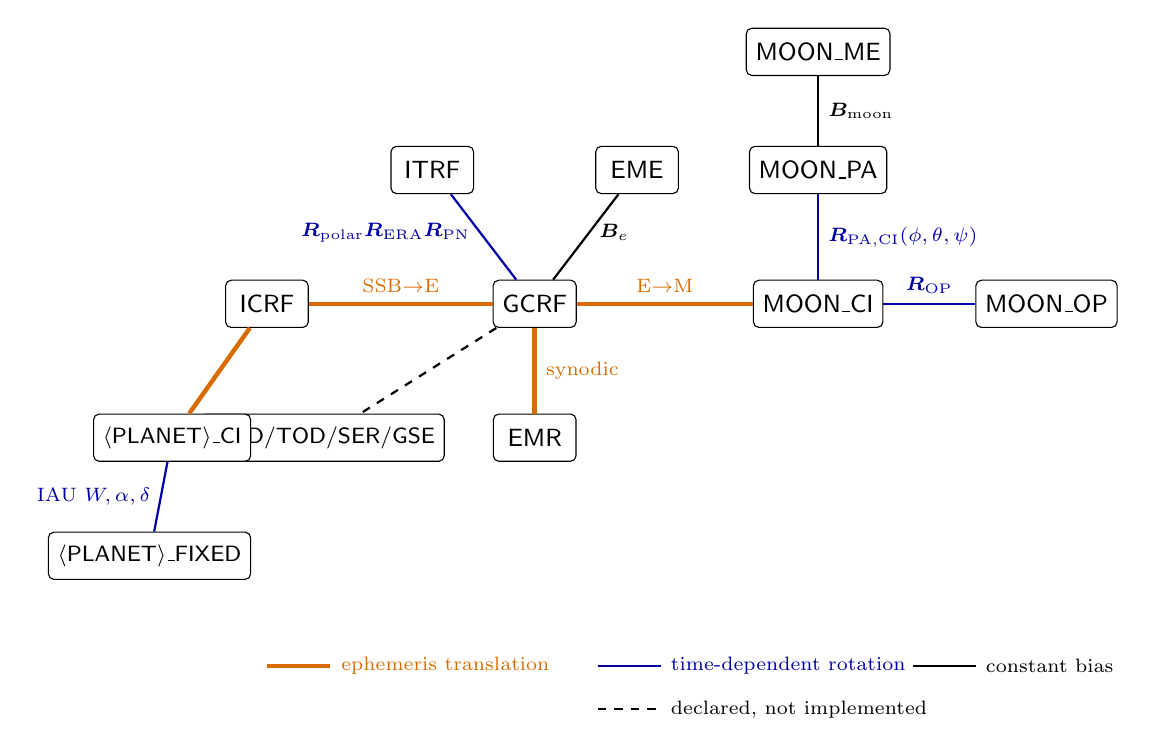
\begin{tikzpicture}[node distance=8mm]
    % --- hubs ---------------------------------------------------------
    \node[tsnode] (icrf)  at (0,0)     {ICRF};
    \node[tsnode] (gcrf)  at (3.4,0)   {GCRF};
    \node[tsnode] (mci)   at (7.0,0)   {MOON\_CI};
    % --- Earth family -------------------------------------------------
    \node[tsnode] (itrf)  at (2.1,1.7)  {ITRF};
    \node[tsnode] (eme)   at (4.7,1.7)  {EME};
    \node[tsnode] (emr)   at (3.4,-1.7) {EMR};
    \node[tsnode] (nyi)   at (0.7,-1.7) {\footnotesize MOD/TOD/SER/GSE};
    % --- Moon family --------------------------------------------------
    \node[tsnode] (mpa)   at (7.0,1.7)  {MOON\_PA};
    \node[tsnode] (mme)   at (7.0,3.2)  {MOON\_ME};
    \node[tsnode] (mop)   at (9.9,0)    {MOON\_OP};
    % --- planets ------------------------------------------------------
    \node[tsnode] (pci)   at (-0.2,-1.7) [anchor=east] {\footnotesize $\langle$PLANET$\rangle$\_CI};
    \node[tsnode] (pfx)   at (-0.2,-3.2) [anchor=east] {\footnotesize $\langle$PLANET$\rangle$\_FIXED};
    % --- edges --------------------------------------------------------
    \draw[model]    (icrf) -- node[above,font=\scriptsize] {SSB$\to$E} (gcrf);
    \draw[model]    (gcrf) -- node[above,font=\scriptsize] {E$\to$M} (mci);
    \draw[linear]   (gcrf) -- node[left,font=\scriptsize,pos=0.55] {$\mat{R}_{\mathrm{polar}}\mat{R}_{\mathrm{ERA}}\mat{R}_{\mathrm{PN}}$} (itrf);
    \draw[constant] (gcrf) -- node[right,font=\scriptsize,pos=0.55] {$\mat{B}_e$} (eme);
    \draw[model]    (gcrf) -- node[right,font=\scriptsize] {synodic} (emr);
    \draw[linear]   (mci)  -- node[right,font=\scriptsize] {$\mat{R}_{\mathrm{PA},\mathrm{CI}}(\phi,\theta,\psi)$} (mpa);
    \draw[constant] (mpa)  -- node[right,font=\scriptsize] {$\mat{B}_{\mathrm{moon}}$} (mme);
    \draw[linear]   (mci)  -- node[above,font=\scriptsize] {$\mat{R}_{\mathrm{OP}}$} (mop);
    \draw[model]    (icrf) -- (pci);
    \draw[linear]   (pci)  -- node[left,font=\scriptsize] {IAU $W,\alpha,\delta$} (pfx);
    \draw[table]    (gcrf) -- (nyi);
    % --- legend -------------------------------------------------------
    \begin{scope}[shift={(0,-4.6)}]
      \draw[model]    (0,0)   -- (0.8,0)   node[right,font=\scriptsize] {ephemeris translation};
      \draw[linear]   (4.2,0) -- (5.0,0)   node[right,font=\scriptsize] {time-dependent rotation};
      \draw[constant] (8.2,0) -- (9.0,0)   node[right,font=\scriptsize] {constant bias};
      \draw[table]    (4.2,-0.55) -- (5.0,-0.55) node[right,font=\scriptsize] {declared, not implemented};
    \end{scope}
  \end{tikzpicture}
  \caption{The implemented frame graph. ICRF, GCRF and MOON\_CI are the
    three hubs; every conversion is routed as a path through them. Edge
    style encodes the nature of the transformation.}
  \label{fig:fc-graph}
\end{figure}

Solar-system planet frames are peeled off first, because they need the ICRF
hub rather than the GCRF one, and because a same-body \code{<PLANET>\_CI}
$\leftrightarrow$ \code{<PLANET>\_FIXED} pair must \emph{not} round-trip
through the barycenter --- doing so would add and subtract a
$\sim\SI{1e11}{\meter}$ vector and destroy the precision of a small
body-relative state.

\begin{lstlisting}[language=cpp, caption={The routing switch and the
  planet-frame fast path
  (\texttt{cpp/lupnt/conversions/frame\_converter.cc}).},
  label={lst:fc-route}]
// cpp/lupnt/conversions/frame_converter.cc :: ConvertFrameBase
template <int N>
Vec<N> ConvertFrameBase(Real t_tdb, const Vec<N>& rv_in, Frame frame_in, Frame frame_out) {
  if (frame_in == frame_out) return rv_in;
  if (IsPlanetFrame(frame_in) || IsPlanetFrame(frame_out))
    return ConvertPlanetFrame(t_tdb, rv_in, frame_in, frame_out);
  switch (frame_in) {
    case Frame::ICRF:
      return ConvertFrame(t_tdb, IcrfToGcrf(t_tdb, rv_in), Frame::GCRF, frame_out);
    case Frame::ITRF:
      return ConvertFrame(t_tdb, ItrfToGcrf(t_tdb, rv_in), Frame::GCRF, frame_out);
    case Frame::GCRF:
      switch (frame_out) {
        case Frame::ICRF: return GcrfToIcrf(t_tdb, rv_in);
        case Frame::ITRF: return GcrfToItrf(t_tdb, rv_in);
        case Frame::EMR:  return GcrfToEmr(t_tdb, rv_in);
        case Frame::EME:  return GcrfToEme(rv_in);
        case Frame::SER: case Frame::GSE:
        case Frame::MOD: case Frame::TOD: throw std::runtime_error("Not implemented");
        case Frame::MOON_PA: case Frame::MOON_ME: case Frame::MOON_OP: case Frame::MOON_CI:
          return ConvertFrame(t_tdb, GcrfToMoonCi(t_tdb, rv_in), Frame::MOON_CI, frame_out);
        default: throw std::runtime_error("Not implemented");
      }
    case Frame::MOON_CI:
      switch (frame_out) {
        case Frame::MOON_OP: return MoonCiToOp(t_tdb, rv_in);
        case Frame::MOON_PA: return MoonCiToPa(t_tdb, rv_in);
        case Frame::MOON_ME: return MoonPaToMe(MoonCiToPa(t_tdb, rv_in));
        default: return ConvertFrame(t_tdb, MoonCiToGcrf(t_tdb, rv_in), Frame::GCRF, frame_out);
      }
    // ... MOON_ME / MOON_PA / MOON_OP / EME / EMR hop back to their hub ...
  }
}
\end{lstlisting}

\begin{lstlisting}[language=cpp, caption={Same-body fast path for planet
  frames (\texttt{cpp/lupnt/conversions/frame\_converter.cc}).},
  label={lst:fc-planetroute}]
// cpp/lupnt/conversions/frame_converter.cc :: ConvertPlanetFrame
if (IsPlanetFrame(frame_in) && IsPlanetFrame(frame_out)
    && GetFrameCenter(frame_in) == GetFrameCenter(frame_out)) {
  BodyId body = GetFrameCenter(frame_in);
  bool in_fixed = IsPlanetFixedFrame(frame_in);
  bool out_fixed = IsPlanetFixedFrame(frame_out);
  if (in_fixed == out_fixed) return rv_in;            // CI<->CI or FIXED<->FIXED
  if (out_fixed) return BodyCiToFixed(t_tdb, rv_in, body);
  return BodyFixedToCi(t_tdb, rv_in, body);
}
\end{lstlisting}

Because the routing is recursive, a conversion such as ITRF $\to$ MOON\_ME
is realised as the composition
ITRF $\to$ GCRF $\to$ MOON\_CI $\to$ MOON\_PA $\to$ MOON\_ME, i.e.\ four
elementary steps, each contributing its own rotation and, where applicable,
its own $\dot{\mat{R}}\vec{r}$ term.

\section{ICRF and GCRF}
\label{sec:fc-icrf}

GCRF and ICRF share axes and differ only in origin. With
$\vec{r}_{\mathrm{SSB}\to E}$ and $\vec{v}_{\mathrm{SSB}\to E}$ the
barycentric state of the Earth from DE440 \citep{park2021de440}, expressed in
GCRF (= ICRS) axes,
%
\begin{equation}
  \label{eq:fc-icrf}
  \vec{r}_{\mathrm{ICRF}} = \vec{r}_{\mathrm{GCRF}} + \vec{r}_{\mathrm{SSB}\to E},
  \qquad
  \vec{v}_{\mathrm{ICRF}} = \vec{v}_{\mathrm{GCRF}} + \vec{v}_{\mathrm{SSB}\to E},
\end{equation}
%
so $\mat{R}_{\mathrm{ICRF},\mathrm{GCRF}} = \mat{I}$ and
$\vec{p}_{\mathrm{ICRF},\mathrm{GCRF}} = \vec{r}_{\mathrm{SSB}\to E}$; the
inverse subtracts the same state. This is a purely kinematic
(Newtonian) origin shift: no relativistic scale factor between TCB-based and
TCG-based coordinates is applied, which is the correct choice given that
\lupnt{}'s states are TDB-compatible throughout.

\section{GCRF and ITRF}
\label{sec:fc-itrf}

This is the only conversion in \lupnt{} that involves three different time
scales simultaneously. It follows the IAU 2006/2000A CIO-based convention
\citep{iers2010}, factored into the product of three rotations:
%
\begin{equation}
  \label{eq:fc-itrf-chain}
  \mat{R}_{\mathrm{ITRF},\mathrm{GCRF}}(t)
  =
  \underbrace{\mat{R}_{\mathrm{polar}}\!\left(t_{\TT}, x_p, y_p\right)}_{\text{polar motion}}
  \;
  \underbrace{\mat{R}_{\mathrm{ERA}}\!\left(t_{\UTone}\right)}_{\text{Earth rotation}}
  \;
  \underbrace{\mat{R}_{\mathrm{PN}}\!\left(t_{\TT}\right)}_{\text{bias--precession--nutation}} .
\end{equation}
%
Read right to left: a GCRF vector is first carried into the Celestial
Intermediate Reference System, then rotated about the Celestial Intermediate
Pole (CIP) through the Earth Rotation Angle into the Terrestrial
Intermediate Reference System, and finally tilted onto the ITRF pole by
polar motion.

\subsection{Bias, precession and nutation}

\lupnt{} does not evaluate the classical precession and nutation angle
series. It reads the CIP unit-vector coordinates $X, Y$ and the CIO locator
$s$ from a tabulated IAU 2006/2000A (SOFA) series
(\file{cpp/lupnt/interfaces/iau_sofa.cc}, one row per day in arcseconds
against Julian date TT, interpolated with a ninth-order Lagrange
polynomial), and assembles the celestial-to-intermediate matrix in closed
form:
%
\begin{equation}
  \label{eq:fc-pn}
  \mat{R}_{\mathrm{PN}}
  =
  \mat{R}_z(-s)
  \begin{bmatrix}
    1-aX^2 & -aXY   & -X \\
    -aXY   & 1-aY^2 & -Y \\
    X      & Y      & 1-a\left(X^2+Y^2\right)
  \end{bmatrix},
  \qquad
  a = \frac{1}{1+\sqrt{1-X^2-Y^2}} .
\end{equation}
%
Here $X = \sin d\cos E$ and $Y = \sin d\sin E$ are the direction cosines of
the CIP in the GCRS, $d$ and $E$ being its polar coordinates, and $s$ is the
CIO locator that positions the Celestial Intermediate Origin on the
intermediate equator. Because the frame bias (the offset between the GCRS
pole/origin and the mean pole/equinox of J2000) is already folded into the
tabulated $X, Y, s$, \cref{eq:fc-pn} is a \emph{bias--precession--nutation}
matrix: no separate bias factor appears in \cref{eq:fc-itrf-chain}. The
argument is $t_{\TT}$, obtained as
$t_{\TT} = \code{ConvertTime}(t_{\TDB}, \TDB, \TT)$ and converted to a
Julian date.

\subsection{Earth rotation}

$\mat{R}_{\mathrm{ERA}} = \mat{R}_z(\theta_{\mathrm{ERA}})$ is a rotation
about the CIP through the Earth Rotation Angle, which is \emph{exactly}
linear in UT1 by definition \citep{iers2010}:
%
\begin{equation}
  \label{eq:fc-era}
  \theta_{\mathrm{ERA}}(t_{\UTone})
  =
  2\pi\left(0.7790572732640 + 1.00273781191135448\, D_{\UTone}\right),
  \qquad
  D_{\UTone} = \frac{t_{\UTone}}{\SI{86400}{\second}},
\end{equation}
%
with $D_{\UTone}$ the number of UT1 days elapsed since J2000; the result is
wrapped to $(-\pi,\pi]$. UT1 itself is recovered in one of two ways: if a
SPICE-fitted EOP model covers the epoch (\cref{sec:fc-spicefit}), then
$t_{\UTone} = t_{\UTC} + (\UTone-\UTC)_{\text{fitted}}$; otherwise the
generic $\TDB\to\UTone$ conversion of \cref{chap:time-conversions} is used,
which interpolates the bundled IERS EOP~14~C04 table.

$\theta_{\mathrm{ERA}}$ is the only factor of \cref{eq:fc-itrf-chain} whose
derivative is retained. Its rate is the Earth rotation rate
$\omega_\oplus \approx \SI{7.292115e-5}{\radian\per\second}$, computed as
%
\begin{equation}
  \label{eq:fc-omega-earth}
  \omega_\oplus =
  \begin{cases}
    \dfrac{2\pi \times 1.00273781191135448}{\SI{86400}{\second}}
      \left(1 + \dfrac{\dd(\UTone-\UTC)}{\dd t}\right)
      & \text{fitted EOP available,}\\[3.2ex]
    \num{7.292115146706979e-5}\left(1 - \dfrac{\mathrm{LOD}}{\SI{86400}{\second}}\right)
      & \text{otherwise,}
  \end{cases}
\end{equation}
%
where LOD is the excess length of day in seconds interpolated from the EOP
table at UTC. In the fitted branch the derivative of $\UTone-\UTC$ is
obtained analytically by differentiating the Chebyshev polynomial, so it is
exact rather than a finite difference.

\subsection{Polar motion}

$\mat{R}_{\mathrm{polar}}$ carries the CIP onto the ITRF pole using the pole
offsets $x_p, y_p$ (radians, from the fitted EOP or interpolated from the
bundled table at UTC) and the TIO locator $s'$:
%
\begin{equation}
  \label{eq:fc-polar}
  \mat{R}_{\mathrm{polar}}
  = \mat{R}_x(-y_p)\,\mat{R}_y(-x_p)\,\mat{R}_z(s'),
  \qquad
  s' = -47\,\mu''\,T,
  \qquad
  T = \frac{t_{\TT}[\si{\second}]}{86400 \times 36525},
\end{equation}
%
where $T$ is the number of Julian centuries of TT elapsed since J2000, as the
IERS definition of the TIO locator requires \citep[Eq.~(5.13)]{iers2010}.
\lupnt{} carries $t_{\TT}$ as seconds past J2000, so the conversion divides by
\code{DAYS\_CENTURY}~$\times$~\code{SECS\_DAY}. The evaluation is factored into
a single file-local helper, templated on the scalar type so that the
\cpp{Real} caller keeps its autodiff derivative and the \cpp{double} caller
stays plain arithmetic:

\begin{lstlisting}[language=cpp, caption={The one place the TIO locator is
  evaluated (\texttt{cpp/lupnt/conversions/frame\_conversions.cc}).},
  label={lst:fc-tio}]
// cpp/lupnt/conversions/frame_conversions.cc :: TioLocator
template <typename T> inline T TioLocator(const T& t_tt) {
  return -47e-6 * RAD_ARCSEC * (t_tt / (DAYS_CENTURY * SECS_DAY));
}
\end{lstlisting}

\begin{lupntnote}
  Both the division by \code{SECS\_DAY} and the fact that there is only one
  copy of \cref{lst:fc-tio} are corrections. The expression previously divided
  by \code{DAYS\_CENTURY} alone, treating seconds as days: the argument was
  $t_{\TT}[\si{\second}]/36525$ instead of
  $t_{\TT}[\si{\second}]/(86400\times36525)$, inflating $s'$ by a factor of
  $\num{86400}$. By the mid-2020s that gave $s' \approx \num{4.9e-6}$~rad in
  place of the intended $\num{5.7e-11}$~rad --- since $s'$ enters
  $\mat{R}_z$ alongside $\theta_{\mathrm{ERA}}$, about \SI{31}{\meter} of
  spurious rotation about the polar axis at the equator.

  The more useful lesson is why it went unnoticed for so long. The formula was
  written out in \emph{three} places: \cpp{RotPolarMotion}, which applies
  $s'$; \cpp{ComputeEopFromSpice} (\cref{sec:fc-spicefit}), which subtracts it
  again when inverting SPICE for the ERA; and a hardcoded copy inside the
  round-trip test in \file{cpp/test/conversions/test_frame_conversions.cc}. In
  that round trip $s'$ cancels identically --- one site removes exactly what
  the other re-applies --- so the test only ever verified that the copies
  \emph{agreed with each other}. It would have passed for any value of $s'$
  whatsoever, including zero, which is precisely how a wrong one survived.
  The two library sites are now the single helper of \cref{lst:fc-tio}; the
  test keeps its own independent expression on purpose, since a test that
  called the helper would verify nothing. Collapsing the duplicates removes the
  possibility of disagreement but not the possibility of a shared error, so the
  magnitude itself is now pinned separately by
  \code{conversions.frame\_conversions\_extra.tio\_locator\_magnitude} in
  \file{cpp/test/conversions/test_frame_conversions_extra.cc}, which recovers
  $s'$ from $\mat{R}_{\mathrm{polar}}$ and bounds it at
  $\num{1e-8}$~rad --- orders of magnitude away from both the correct value and
  the old one.
\end{lupntnote}

\subsection{The complete mapping and its inverse}

The position and velocity mapping is
%
\begin{align}
  \label{eq:fc-itrf-rv}
  \vec{r}_{\mathrm{ITRF}} &= \mat{R}_{\mathrm{ITRF},\mathrm{GCRF}}\,\vec{r}_{\mathrm{GCRF}}, \\
  \vec{v}_{\mathrm{ITRF}} &= \mat{R}_{\mathrm{ITRF},\mathrm{GCRF}}\,\vec{v}_{\mathrm{GCRF}}
    + \dot{\mat{R}}_{\mathrm{ITRF},\mathrm{GCRF}}\,\vec{r}_{\mathrm{GCRF}},
  \nonumber
\end{align}
%
where only the sidereal factor is differentiated,
%
\begin{equation}
  \label{eq:fc-itrf-rdot}
  \dot{\mat{R}}_{\mathrm{ITRF},\mathrm{GCRF}}
  = \mat{R}_{\mathrm{polar}}\,\dot{\mat{R}}_{\mathrm{ERA}}\,\mat{R}_{\mathrm{PN}} .
\end{equation}
%
Applying \cref{eq:fc-omega} to \cref{eq:fc-itrf-rdot} and using
$\dot{\mat{R}}_{\mathrm{ERA}}\mat{R}_{\mathrm{ERA}}\transpose
= -\left[\omega_\oplus\uvec{z}\right]_\times$ gives
%
\begin{equation}
  \label{eq:fc-itrf-omega}
  \dot{\mat{R}}_{\mathrm{ITRF},\mathrm{GCRF}}\,
  \mat{R}_{\mathrm{ITRF},\mathrm{GCRF}}\transpose
  = -\left[\vec{\omega}_\oplus\right]_\times,
  \qquad
  \vec{\omega}_\oplus = \omega_\oplus\, \mat{R}_{\mathrm{polar}}\uvec{z},
\end{equation}
%
so \cref{eq:fc-itrf-rv} is exactly the classical
$\vec{v}_{\mathrm{ITRF}} = \mat{R}\vec{v}_{\mathrm{GCRF}}
- \vec{\omega}_\oplus\times\vec{r}_{\mathrm{ITRF}}$ with the spin axis taken
as the polar-motion-corrected CIP direction --- to first order, the ITRF
$z$-axis. Neglecting $\dot{\mat{R}}_{\mathrm{PN}}$ and
$\dot{\mat{R}}_{\mathrm{polar}}$ discards precession--nutation rates of
order $\num{1e-12}$~rad/s and polar-motion rates of order $\num{1e-13}$~rad/s,
seven to eight orders of magnitude below $\omega_\oplus$; see
\cref{sec:fc-boundaries} for the resulting velocity error.

The inverse solves \cref{eq:fc-itrf-rv} for the GCRF state, reusing the
already-computed $\vec{r}_{\mathrm{GCRF}}$ in the transport term:
%
\begin{align}
  \label{eq:fc-itrf-inv}
  \vec{r}_{\mathrm{GCRF}} &= \mat{R}_{\mathrm{ITRF},\mathrm{GCRF}}\transpose\,\vec{r}_{\mathrm{ITRF}}, \\
  \vec{v}_{\mathrm{GCRF}} &= \mat{R}_{\mathrm{ITRF},\mathrm{GCRF}}\transpose
    \left(\vec{v}_{\mathrm{ITRF}} - \dot{\mat{R}}_{\mathrm{ITRF},\mathrm{GCRF}}\,\vec{r}_{\mathrm{GCRF}}\right).
  \nonumber
\end{align}

\begin{lstlisting}[language=cpp, caption={GCRF to ITRF, rotation product and
  velocity term
  (\texttt{cpp/lupnt/conversions/frame\_conversions.cc}).},
  label={lst:fc-gcrf-itrf}]
// cpp/lupnt/conversions/frame_conversions.cc :: GcrfToItrf
Vec6 GcrfToItrf(Real t_tdb, const Vec6& rv_gcrf) {
  Mat3 R_po    = RotPolarMotion(t_tdb);        // R_polar(t_TT, x_p, y_p)
  Mat3 R_pn    = RotPrecessionNutation(t_tdb); // R_PN(t_TT) from tabulated (X, Y, s)
  Mat3 R_s     = RotSideralMotion(t_tdb);      // R_z(theta_ERA(t_UT1))
  Mat3 R_s_dot = RotSideralMotionDot(t_tdb);   // d/dt of the above

  Mat3 R_GcrfToItrf     = R_po * R_s     * R_pn;
  Mat3 R_GcrfToItrf_dot = R_po * R_s_dot * R_pn;

  Vec3 r_gcrf = rv_gcrf.head(3);
  Vec3 v_gcrf = rv_gcrf.tail(3);
  Vec3 r_itrf = R_GcrfToItrf * r_gcrf;
  Vec3 v_itrf = R_GcrfToItrf * v_gcrf + R_GcrfToItrf_dot * r_gcrf;

  Vec6 rv_itrf;
  rv_itrf << r_itrf, v_itrf;
  return rv_itrf;
}
\end{lstlisting}

\begin{lstlisting}[language=cpp, caption={Precession--nutation from the
  tabulated CIP coordinates
  (\texttt{cpp/lupnt/conversions/frame\_conversions.cc}).},
  label={lst:fc-pn}]
// cpp/lupnt/conversions/frame_conversions.cc :: RotPrecessionNutation
Real t_tt  = ConvertTime(t_tdb, Time::TDB, Time::TT);
Real jd_tt = TimeToJd(t_tt);
IauSofaData iau_data = GetIauSofaData(jd_tt);   // X, Y, s in arcsec
Real X = iau_data.X * RAD_ARCSEC;
Real Y = iau_data.Y * RAD_ARCSEC;
Real s = iau_data.s * RAD_ARCSEC;
Real a = 1. / (1. + sqrt(1. - X * X - Y * Y));
Mat3 mat{{1. - a * X * X, -a * X * Y,     -X},
         {-a * X * Y,     1. - a * Y * Y, -Y},
         {X,              Y,              1. - a * (X * X + Y * Y)}};
Mat3 R_pn = RotZ(-s) * mat;
\end{lstlisting}

\begin{lupntnote}
  The \cpp{Vec3} (position-only) overloads of \cpp{GcrfToItrf} and
  \cpp{ItrfToGcrf} skip \cpp{RotSideralMotionDot} entirely. They are
  therefore cheaper by one EOP lookup, and are the right entry point for
  static ground-station coordinates.
\end{lupntnote}

\subsection{Equinox-based sidereal angles}

\lupnt{} also provides the classical equinox-based angles in
\file{cpp/lupnt/conversions/time_conversions.cc}, but they are \emph{not}
used by \cpp{GcrfToItrf}. Greenwich Mean Sidereal Time is evaluated from the
IAU-82 polynomial,
%
\begin{equation}
  \label{eq:fc-gmst}
  \begin{aligned}
    \theta_{\mathrm{GMST}}
      &= 2\pi \operatorname{frac}\!\left(\frac{g}{\SI{86400}{\second}}\right), \\
    g &= 24110.54841 + 8640184.812866\,T_0
         + 1.002737909350795\,u
         + \left(0.093104 - \num{6.2e-6}\,T\right)T^2,
  \end{aligned}
\end{equation}
%
with $T_0$ the Julian centuries from J2000 to UT1 midnight of the day in
question, $u$ the seconds of UT1 elapsed since that midnight, and $T$ the
Julian centuries from J2000 to the epoch itself; Greenwich Apparent Sidereal
Time adds the equation of the equinoxes,
%
\begin{equation}
  \label{eq:fc-gast}
  \theta_{\mathrm{GAST}} = \theta_{\mathrm{GMST}} + \Delta\psi\cos\varepsilon
  \pmod{2\pi}.
\end{equation}
%
GAST is used by the Sun/Moon analytic ephemeris helper
(\file{cpp/lupnt/environment/solar_system.cc}, which builds
$\mat{R}_z(\theta_{\mathrm{GAST}})$), and both angles are cross-validated
against Orekit. Because \cref{eq:fc-itrf-chain} is CIO-based, the equinox
route and the CIO route are alternative --- not composable --- descriptions
of the same physical rotation.

\section{GCRF and EME2000}
\label{sec:fc-eme}

EME2000 (also called J2000 or, in the enum, \code{ECI}) is the mean equator
and equinox of J2000. It differs from GCRF by the constant IAU 2006 frame
bias:
%
\begin{equation}
  \label{eq:fc-bias}
  \mat{B}_e \equiv \mat{R}_{\mathrm{EME},\mathrm{GCRF}}
  = \mat{R}_x(-\eta_0)\,\mat{R}_y(\xi_0)\,\mat{R}_z(\Delta\alpha_0),
\end{equation}
%
with the three bias angles taken from
\file{cpp/lupnt/core/constants.h},
%
\begin{equation}
  \label{eq:fc-bias-angles}
  \xi_0 = -16.6170\ \mathrm{mas}, \qquad
  \eta_0 = -6.8192\ \mathrm{mas}, \qquad
  \Delta\alpha_0 = -14.6\ \mathrm{mas},
\end{equation}
%
where $\xi_0, \eta_0$ are the celestial-pole offsets at J2000 and
$\Delta\alpha_0$ is the right-ascension offset of the GCRS origin from the
mean equinox \citep{iers2010}. \Cref{eq:fc-bias} is exact to all orders in
the angles because it is a genuine product of elementary rotations; the
first- and second-order approximations are also available for comparison,
%
\begin{equation}
  \label{eq:fc-bias-first}
  \mat{B}_e \approx
  \begin{bmatrix}
    1 & \Delta\alpha_0 & -\xi_0 \\
    -\Delta\alpha_0 & 1 & -\eta_0 \\
    \xi_0 & \eta_0 & 1
  \end{bmatrix}
  \quad (\cpp{RotGcrfToEmeFirstOrder}),
\end{equation}
%
with \cpp{RotGcrfToEmeSecondOrder} retaining the quadratic terms. Since
$\mat{B}_e$ is constant, $\dot{\mat{B}}_e = \mat{0}$ and the same matrix is
applied to position and velocity; the inverse is
$\mat{B}_e\transpose$. Neither \cpp{GcrfToEme} nor \cpp{EmeToGcrf} takes an
epoch argument.

\section{The Earth--Moon rotating frame}
\label{sec:fc-emr}

\code{EMR} is a synodic frame built on the instantaneous Earth$\to$EMB
(Earth--Moon barycenter) state $(\vec{r}_c, \vec{v}_c)$ taken from DE440 in
GCRF axes. Its basis is
%
\begin{equation}
  \label{eq:fc-emr-basis}
  \uvec{x} = \frac{\vec{r}_c}{\lVert\vec{r}_c\rVert},
  \qquad
  \uvec{n} = \frac{\vec{r}_c\times\vec{v}_c}{\lVert\vec{r}_c\times\vec{v}_c\rVert},
  \qquad
  \uvec{y} = \uvec{n}\times\uvec{x},
\end{equation}
%
and the rotation from GCRF to EMR stacks these as rows in the order
$(\uvec{x}, \uvec{y}, \uvec{n})$, so the EMR components of a vector are
(radial, in-track, orbit-normal). The transform of a GCRF state
$(\vec{r}_d,\vec{v}_d)$ is
%
\begin{equation}
  \label{eq:fc-emr}
  \vec{r}_{\mathrm{EMR}} = \mat{R}\left(\vec{r}_d - \vec{r}_c\right),
  \qquad
  \vec{v}_{\mathrm{EMR}} = \mat{R}\left(\vec{v}_d - \vec{v}_c
    - \vec{\omega}\times\left(\vec{r}_d - \vec{r}_c\right)\right),
\end{equation}
%
implemented by \cpp{InertialToSynodic} /\cpp{SynodicToInertial} in
\file{cpp/lupnt/conversions/state_conversions.cc}, which \cpp{GcrfToEmr} and
\cpp{EmrToGcrf} wrap. The origin of EMR is therefore the EMB, not the Earth.

\begin{lupntwarning}
  \cpp{InertialToSynodic} forms the frame angular velocity as
  $\vec{\omega} = (\vec{r}_c\times\vec{v}_c)/\lVert\vec{r}_c\rVert$, whereas
  the angular velocity of the rotating frame is
  $\vec{\omega} = (\vec{r}_c\times\vec{v}_c)/\lVert\vec{r}_c\rVert^2$. The
  transport term in \cref{eq:fc-emr} is consequently scaled by
  $\lVert\vec{r}_c\rVert$. EMR \emph{positions} are unaffected (they do not
  involve $\vec{\omega}$); EMR \emph{velocities} should not be relied on
  until this is reconciled. The \cpp{Vec3} overloads zero the velocity
  before calling through, so they return correct positions.
\end{lupntwarning}

\section{GCRF and MOON\_CI}
\label{sec:fc-moonci}

\code{MOON\_CI} is Moon-centered and axis-aligned with GCRF/ICRF: the
conversion is a pure translation by the geocentric Moon state, evaluated
from the DE440 Chebyshev coefficients \citep{park2021de440} bundled with
\lupnt{} (\file{cpp/lupnt/interfaces/kernels.cc}). With
$\vec{r}_{E\to M}, \vec{v}_{E\to M}$ the Moon state relative to Earth in
GCRF axes,
%
\begin{equation}
  \label{eq:fc-moonci}
  \vec{r}_{\mathrm{MOON\_CI}} = \vec{r}_{\mathrm{GCRF}} - \vec{r}_{E\to M},
  \qquad
  \vec{v}_{\mathrm{MOON\_CI}} = \vec{v}_{\mathrm{GCRF}} - \vec{v}_{E\to M},
\end{equation}
%
so $\mat{R}_{\mathrm{MOON\_CI},\mathrm{GCRF}} = \mat{I}$ and
$\vec{p} = -\vec{r}_{E\to M}$. The velocity is the analytic derivative of
the position Chebyshev series, not a finite difference.

\begin{lstlisting}[language=cpp, caption={GCRF to Moon-centered inertial ---
  a pure DE440 translation
  (\texttt{cpp/lupnt/conversions/frame\_conversions.cc}).},
  label={lst:fc-moonci}]
// cpp/lupnt/conversions/frame_conversions.cc :: GcrfToMoonCi
Vec6 GcrfToMoonCi(Real t_tdb, const Vec6& rv_gcrf) {
  Vec6 rv_earth2moon = GetBodyPosVel(t_tdb, BodyId::EARTH, BodyId::MOON, Frame::GCRF);
  Vec6 rv_mi = rv_gcrf - rv_earth2moon;
  return rv_mi;
}
\end{lstlisting}

\section{MOON\_CI and MOON\_PA}
\label{sec:fc-moonpa}

\code{MOON\_PA} is the lunar principal-axis (mantle) frame. Its orientation
relative to the inertial axes is given by the three Euler angles of the
lunar physical libration, $\phi$ (node), $\theta$ (inclination of the
principal-axis equator) and $\psi$ (rotation), which DE440 supplies as a
Chebyshev series in the same file as the planetary positions
(\cpp{GetLunarMantleData}, ephemeris item
\code{MOON\_MANTLE\_LIBRATIONS}). The rotation is the classical
$Z$--$X$--$Z$ sequence
%
\begin{equation}
  \label{eq:fc-moonpa}
  \mat{R}_{\mathrm{PA},\mathrm{CI}}(t)
  = \mat{R}_z\!\left(\psi(t)\right)\,
    \mat{R}_x\!\left(\theta(t)\right)\,
    \mat{R}_z\!\left(\phi(t)\right),
\end{equation}
%
whose exact derivative follows from the product rule and the elementary
derivative matrices of \cref{eq:fc-elementary}:
%
\begin{equation}
  \label{eq:fc-moonpa-dot}
  \dot{\mat{R}}_{\mathrm{PA},\mathrm{CI}}
  = \mat{R}_z'(\psi,\dot\psi)\,\mat{R}_x(\theta)\,\mat{R}_z(\phi)
  + \mat{R}_z(\psi)\,\mat{R}_x'(\theta,\dot\theta)\,\mat{R}_z(\phi)
  + \mat{R}_z(\psi)\,\mat{R}_x(\theta)\,\mat{R}_z'(\phi,\dot\phi).
\end{equation}
%
The angle rates $\dot\phi,\dot\theta,\dot\psi$ come from differentiating the
same Chebyshev series, so \cref{eq:fc-moonpa-dot} is exact (subject to the
ephemeris fit), not a numerical derivative. Unlike the Earth case, no term
is dropped: the lunar rotation rate
($\approx\SI{2.66e-6}{\radian\per\second}$) and the libration rates are of
comparable smallness, so retaining all three products matters. The state
transform and its inverse are
%
\begin{align}
  \label{eq:fc-moonpa-vel}
  \vec{r}_{\mathrm{PA}} &= \mat{R}_{\mathrm{PA},\mathrm{CI}}\,\vec{r}_{\mathrm{CI}},
  &\vec{v}_{\mathrm{PA}} &= \mat{R}_{\mathrm{PA},\mathrm{CI}}\,\vec{v}_{\mathrm{CI}}
    + \dot{\mat{R}}_{\mathrm{PA},\mathrm{CI}}\,\vec{r}_{\mathrm{CI}}, \\
  \vec{r}_{\mathrm{CI}} &= \mat{R}_{\mathrm{PA},\mathrm{CI}}\transpose\,\vec{r}_{\mathrm{PA}},
  &\vec{v}_{\mathrm{CI}} &= \mat{R}_{\mathrm{PA},\mathrm{CI}}\transpose
    \left(\vec{v}_{\mathrm{PA}} - \dot{\mat{R}}_{\mathrm{PA},\mathrm{CI}}\,\vec{r}_{\mathrm{CI}}\right).
  \nonumber
\end{align}

\begin{lstlisting}[language=cpp, caption={Lunar libration rotation and its
  analytic derivative
  (\texttt{cpp/lupnt/conversions/frame\_conversions.cc}).},
  label={lst:fc-moonpa}]
// cpp/lupnt/conversions/frame_conversions.cc :: RotMoonCiToPa
Vec6 lunar_mantle = GetLunarMantleData(t_tdb, compute_vel);
auto [phi, theta, psi, phi_dot, theta_dot, psi_dot] = Unpack(lunar_mantle);

Mat3 R_z_phi = RotZ(phi), R_x_theta = RotX(theta), R_z_psi = RotZ(psi);
Mat3 R_mi2pa = R_z_psi * R_x_theta * R_z_phi;

if (compute_vel) {
  *R_mi2pa_dot = RotZdot(psi, psi_dot) * R_x_theta          * R_z_phi
               + R_z_psi               * RotXdot(theta, theta_dot) * R_z_phi
               + R_z_psi               * R_x_theta          * RotZdot(phi, phi_dot);
}
\end{lstlisting}

Two implementation details are worth recording. First,
\cpp{GetLunarMantleData} divides the raw ephemeris item by
\code{M\_KM}~$=\num{1e3}$, undoing the kilometre-to-metre scaling that the
generic Chebyshev reader applies to \emph{position} items, so the returned
angles are radians and the rates are \si{\radian\per\second}. Second,
\cpp{RotMoonCiToPa} caches the last evaluated $(\mat{R},\dot{\mat{R}})$ pair
keyed on the epoch, because a single \cpp{ConvertFrame} call from a
lunar-fixed frame to an Earth frame can request it several times.

\begin{lupntnote}
  The \code{M\_KM} division above is applied \emph{once}, in the scalar
  \cpp{GetLunarMantleData(Real, bool)} overload. The vectorised overload
  \cpp{GetLunarMantleData(VecX, bool)} in
  \file{cpp/lupnt/interfaces/kernels.cc} used to divide the scalar overload's
  return value by \code{M\_KM} a second time, so every libration angle it
  produced was $\num{1e3}$ too small: at one sample epoch it returned
  $\phi = \num{-5.41e-5}$ where the scalar overload returned
  $\num{-5.41e-2}$. The defect was latent --- nothing inside \lupnt{} routes
  \cref{eq:fc-moonpa} through the vector overload, so no \code{MOON\_PA}
  result was ever wrong --- but the overload is declared public API in
  \file{cpp/lupnt/interfaces/kernels.h}, so any external caller batching
  epochs would have received silently wrong angles. The
  extra division has been removed, and the two overloads are now required to
  agree row for row by
  \code{interfaces.kernels\_extra.lunar\_mantle\_vector\_matches\_scalar} in
  \file{cpp/test/interfaces/test_kernels_extra.cc}.
\end{lupntnote}

\begin{lupntnote}
  If \cpp{InitFrameConversionFromSpice} has fitted a lunar-orientation model
  covering $t_{\TDB}$, \cpp{TryGetFittedMoonCiToPa} returns the
  SPICE-derived rotation and its exact derivative instead, and the DE
  libration branch is bypassed entirely (\cref{sec:fc-spicefit}).
\end{lupntnote}

\section{MOON\_PA and MOON\_ME}
\label{sec:fc-moonme}

The mean-Earth/polar-axis frame \code{MOON\_ME} --- the frame in which lunar
cartographic products and surface-station coordinates are published --- is
related to the principal-axis frame by a constant bias rotation of three
small angles:
%
\begin{equation}
  \label{eq:fc-moonme}
  \mat{B}_{\mathrm{moon}} \equiv \mat{R}_{\mathrm{ME},\mathrm{PA}}
  = \mat{R}_x(-0.2785'')\,\mat{R}_y(-78.6944'')\,\mat{R}_z(-67.8526'') .
\end{equation}
%
The total angle is about $104''$, i.e.\ roughly \SI{880}{\meter} on the
lunar surface --- large enough that confusing PA and ME coordinates is a
first-order error for any surface user. As with the Earth frame bias, the
same matrix is applied to position and velocity, no epoch is needed, and the
inverse is the transpose.

\section{MOON\_OP: the lunar orbit-plane frame}
\label{sec:fc-moonop}

\code{MOON\_OP} is the frozen-orbit analysis frame: it is Moon-centered,
with its $z$-axis along the Earth--Moon orbital angular momentum and its
$x$-axis the lunar mean-Earth pole projected into that plane. Let
$(\vec{r}_{M\to E}, \vec{v}_{M\to E})$ be the Moon-to-Earth state in GCRF
axes; then
%
\begin{equation}
  \label{eq:fc-moonop-z}
  \uvec{z}_{\mathrm{OP}}
  = \frac{\vec{r}_{M\to E}\times\vec{v}_{M\to E}}
         {\lVert\vec{r}_{M\to E}\times\vec{v}_{M\to E}\rVert},
\end{equation}
%
and with $\uvec{p}$ the \code{MOON\_ME} $z$-axis expressed in
\code{MOON\_CI} (obtained by a recursive \cpp{ConvertFrame} call on
$\uvec{e}_z$),
%
\begin{equation}
  \label{eq:fc-moonop-xy}
  \uvec{x}_{\mathrm{OP}}
  = \frac{\uvec{p}\times\uvec{z}_{\mathrm{OP}}}
         {\lVert\uvec{p}\times\uvec{z}_{\mathrm{OP}}\rVert},
  \qquad
  \uvec{y}_{\mathrm{OP}} = \uvec{z}_{\mathrm{OP}}\times\uvec{x}_{\mathrm{OP}} .
\end{equation}
%
The columns of the OP-to-CI rotation are these three unit vectors expressed
in CI axes,
%
\begin{equation}
  \label{eq:fc-moonop-R}
  \mat{R}_{\mathrm{CI},\mathrm{OP}}
  = \begin{bmatrix}
      \uvec{x}_{\mathrm{OP}} & \uvec{y}_{\mathrm{OP}} & \uvec{z}_{\mathrm{OP}}
    \end{bmatrix},
\end{equation}
%
and \cpp{MoonCiToOp} applies its transpose.

\begin{lstlisting}[language=cpp, caption={Orbit-plane triad
  (\texttt{cpp/lupnt/conversions/frame\_conversions.cc}).},
  label={lst:fc-moonop}]
// cpp/lupnt/conversions/frame_conversions.cc :: RotMoonOpToCi
Vec6 rv_m2e = GetBodyPosVel(t_tdb, BodyId::MOON, BodyId::EARTH, Frame::GCRF);
Vec3 z_op   = rv_m2e.head(3).cross(rv_m2e.tail(3)).normalized();
Vec3 i_pole = ConvertFrame(t_tdb, Vec3::UnitZ(), Frame::MOON_ME, Frame::MOON_CI);
Vec3 x_op   = i_pole.cross(z_op).normalized();
Vec3 y_op   = z_op.cross(x_op).normalized();
Mat3 R_op2ci;
R_op2ci << x_op, y_op, z_op;
\end{lstlisting}

\begin{lupntwarning}
  \cpp{MoonCiToOp}/\cpp{MoonOpToCi} apply $\mat{R}_{\mathrm{CI},\mathrm{OP}}$
  to position \emph{and} velocity with no $\dot{\mat{R}}$ term. The OP frame
  precesses with the lunar orbit at
  $\sim\SI{2.7e-6}{\radian\per\second}$, so an OP velocity omits a transport
  term of order $\omega r$ --- about \SI{5}{\meter\per\second} at
  \SI{2000}{\kilo\meter} selenocentric radius. \code{MOON\_OP} is intended
  for geometric orbit-design work (orbit-plane orientation, frozen-orbit
  elements), not for velocity-critical computation.
\end{lupntwarning}

\section{Solar-system planet frames}
\label{sec:fc-planets}

Each \code{<PLANET>\_CI} frame is planet-centered with ICRF axes; reaching it
from the ICRF hub is a pure ephemeris translation
(\cpp{PlanetCiToIcrf}/\cpp{IcrfToPlanetCi}). Each \code{<PLANET>\_FIXED}
frame co-rotates with the planet under the IAU linear orientation model:
with pole right ascension $\alpha$, pole declination $\delta$, and
prime-meridian angle $W$,
%
\begin{equation}
  \label{eq:fc-iau}
  \mat{R}_{\mathrm{FIXED},\mathrm{CI}}
  = \mat{R}_z(W)\,
    \mat{R}_x\!\left(\tfrac{\pi}{2}-\delta\right)\,
    \mat{R}_z\!\left(\tfrac{\pi}{2}+\alpha\right),
\end{equation}
%
where
%
\begin{equation}
  \label{eq:fc-iau-elements}
  \alpha = \alpha_0 + \dot{\alpha}\,T, \qquad
  \delta = \delta_0 + \dot{\delta}\,T, \qquad
  W = W_0 + \dot{W}\,d,
\end{equation}
%
with $d$ the days and $T = d/36525$ the Julian centuries past J2000 in TT.
The coefficients (\cref{tab:fc-iau}) are the IAU Working Group on
Cartographic Coordinates and Rotational Elements values; the small periodic
terms of the full model are omitted.

\begin{table}[H]
  \centering
  \caption{IAU linear orientation coefficients used by
    \cpp{RotBodyCiToFixed}. Angles in degrees; $T$ in Julian centuries and
    $d$ in days past J2000 (TT).}
  \label{tab:fc-iau}
  \begin{tabular}{l r r r r r r}
    \toprule
    Body & $\alpha_0$ & $\dot{\alpha}$ & $\delta_0$ & $\dot{\delta}$ & $W_0$ & $\dot{W}$ \\
    \midrule
    Mercury & $281.0103$  & $-0.0328$   & $61.4155$  & $-0.0049$ & $329.5988$ & $6.1385108$    \\
    Venus   & $272.76$    & $0$         & $67.16$    & $0$       & $160.20$   & $-1.4813688$   \\
    Mars    & $317.68143$ & $-0.1061$   & $52.88650$ & $-0.0609$ & $176.630$  & $350.89198226$ \\
    Jupiter & $268.056595$& $-0.006499$ & $64.495303$& $0.002413$& $284.95$   & $870.5360000$  \\
    Saturn  & $40.589$    & $-0.036$    & $83.537$   & $-0.004$  & $38.90$    & $810.7939024$  \\
    Uranus  & $257.311$   & $0$         & $-15.175$  & $0$       & $203.81$   & $-501.1600928$ \\
    Neptune & $299.36$    & $0$         & $43.46$    & $0$       & $249.978$  & $541.1397757$  \\
    \bottomrule
  \end{tabular}
\end{table}

Only the prime-meridian spin contributes appreciably to the derivative --- the
pole rates are of order $\SI{0.01}{\degree}$ per century, i.e.\
$\sim\num{1e-16}$~rad/s --- so
%
\begin{equation}
  \label{eq:fc-iau-dot}
  \dot{\mat{R}}_{\mathrm{FIXED},\mathrm{CI}}
  \approx \mat{R}_z'\!\left(W, \dot{W}\right)
    \mat{R}_x\!\left(\tfrac{\pi}{2}-\delta\right)
    \mat{R}_z\!\left(\tfrac{\pi}{2}+\alpha\right),
  \qquad
  \dot{W}\ \text{in \si{\radian\per\second}}.
\end{equation}

\begin{lstlisting}[language=cpp, caption={IAU body orientation
  (\texttt{cpp/lupnt/conversions/frame\_conversions.cc}).},
  label={lst:fc-iau}]
// cpp/lupnt/conversions/frame_conversions.cc :: RotBodyCiToFixed
Real t_tt = ConvertTime(t_tdb, Time::TDB, Time::TT);
Real d = TimeToJd(t_tt) - JD_J2000_TT;  // days past J2000 (TT)
Real T = d / 36525.0;                   // Julian centuries past J2000 (TT)

Real ra  = (o.ra0  + o.ra0_T  * T) * RAD;
Real dec = (o.dec0 + o.dec0_T * T) * RAD;
Real W   = (o.w0   + o.w_dot  * d) * RAD;

Mat3 Rx_pole = RotX(M_PI / 2 - dec);
Mat3 Rz_node = RotZ(M_PI / 2 + ra);
Mat3 R = RotZ(W) * Rx_pole * Rz_node;
if (R_dot != nullptr) {
  Real w_dot = o.w_dot * RAD / SECS_DAY;  // [rad/s]
  *R_dot = RotZdot(W, w_dot) * Rx_pole * Rz_node;
}
\end{lstlisting}

\section{Topocentric frames: ENU and azimuth--elevation--range}
\label{sec:fc-topocentric}

The topocentric helpers in
\file{cpp/lupnt/conversions/coordinate_conversions.cc} operate
\emph{entirely inside one body-fixed frame}; they take a reference position
$\vec{r}_{\mathrm{ref}}$ and a body shape, never a \cpp{Frame} argument. The
caller is responsible for having converted both the target and the reference
into the same body-fixed frame (ITRF for Earth, MOON\_PA or MOON\_ME for the
Moon) with \cpp{ConvertFrame} first.

\paragraph{Geodetic coordinates.} With equatorial radius $R_b$, flattening
$f$, and first eccentricity squared $e^2 = f(2-f)$, the geodetic-to-Cartesian
map is
%
\begin{equation}
  \label{eq:fc-lla}
  \vec{r} =
  \begin{bmatrix}
    (N+h)\cos\varphi\cos\lambda \\
    (N+h)\cos\varphi\sin\lambda \\
    \left((1-e^2)N+h\right)\sin\varphi
  \end{bmatrix},
  \qquad
  N = \frac{R_b}{\sqrt{1-e^2\sin^2\varphi}},
\end{equation}
%
$\varphi$ being geodetic latitude, $\lambda$ longitude and $h$ altitude
above the ellipsoid. The inverse (\cpp{CartToLatLonAlt}) is the classical
fixed-point iteration on $\Delta z = N e^2 \sin\varphi$, iterated to
\code{EPS} and capped at 1000 iterations; passing $R_b = 0$ makes it fall
back to a sphere of radius $\lVert\vec{r}\rVert$.

\paragraph{East--north--up.} The rotation from body-fixed axes to the local
ENU triad at $(\varphi,\lambda)$ is
%
\begin{equation}
  \label{eq:fc-enu-rot}
  \mat{R}_{\mathrm{ENU}}
  = \mat{R}_x\!\left(\tfrac{\pi}{2}-\varphi\right)
    \mat{R}_z\!\left(\tfrac{\pi}{2}+\lambda\right)
  = \begin{bmatrix}
      -\sin\lambda & \cos\lambda & 0 \\
      -\sin\varphi\cos\lambda & -\sin\varphi\sin\lambda & \cos\varphi \\
      \cos\varphi\cos\lambda & \cos\varphi\sin\lambda & \sin\varphi
    \end{bmatrix},
\end{equation}
%
whose rows are the east, north and up unit vectors. The transform of a
state is
%
\begin{equation}
  \label{eq:fc-enu}
  \vec{r}_{\mathrm{ENU}} = \mat{R}_{\mathrm{ENU}}\left(\vec{r}-\vec{r}_{\mathrm{ref}}\right),
  \qquad
  \vec{v}_{\mathrm{ENU}} = \mat{R}_{\mathrm{ENU}}\,\vec{v} .
\end{equation}
%
No $\dot{\mat{R}}$ term appears, and none is needed: $\mat{R}_{\mathrm{ENU}}$
is constant \emph{in the body-fixed frame}, and the input velocity is
already body-fixed-relative. The rotation of the body has been accounted for
once, in the GCRF$\to$ITRF (or MOON\_CI$\to$MOON\_PA) step.

\paragraph{Azimuth, elevation, range.} Finally,
%
\begin{equation}
  \label{eq:fc-azel}
  \rho = \lVert\vec{r}_{\mathrm{ENU}}\rVert, \qquad
  A = \atantwo(e, n), \qquad
  E = \arcsin\!\left(\frac{u}{\rho}\right),
\end{equation}
%
so azimuth is measured clockwise from north and elevation upward from the
local horizon; the inverse is
$(e,n,u) = \rho(\cos E\sin A,\ \cos E\cos A,\ \sin E)$.
\cpp{CartToAzElRange} is the composition of \cref{eq:fc-enu} and
\cref{eq:fc-azel}.

\section{SPICE-calibrated Earth and lunar orientation}
\label{sec:fc-spicefit}

\lupnt{}'s native Earth and lunar orientation models are analytic and
self-contained: an IAU 2006/2000A series plus an IERS EOP table for the
Earth, and DE Chebyshev libration angles for the Moon. Both can disagree
with SPICE's high-accuracy binary PCK products
(\file{earth_latest_high_prec.bpc}, \file{moon_pa_de*.bpc})
\citep{acton1996spice}, most severely when the bundled EOP table does not
cover the requested epoch. \cpp{InitFrameConversionFromSpice} closes that
gap for a known simulation window, without requiring SPICE at evaluation
time.

For the Earth, \cpp{ComputeEopFromSpice} inverts the decomposition
\cref{eq:fc-itrf-chain} at a single epoch. Given SPICE's
\code{"J2000"}$\to$\code{"ITRF93"} rotation $\mat{R}_{\mathrm{SPICE}}$ and
\lupnt{}'s own $\mat{R}_{\mathrm{PN}}$, it forms
$\mat{M} = \mat{R}_{\mathrm{SPICE}}\mat{R}_{\mathrm{PN}}\transpose$ and reads
off
%
\begin{equation}
  \label{eq:fc-eopinv}
  x_p = \arcsin M_{13}, \qquad
  y_p = -\atantwo\!\left(M_{23}, M_{33}\right), \qquad
  s' + \theta_{\mathrm{ERA}} = \atantwo\!\left(M_{12}, M_{11}\right),
\end{equation}
%
then linearises \cref{eq:fc-era} about $t_{\UTone}\approx t_{\TDB}$ to
recover $\UTone-\UTC$ (valid because the true offset is at most about
\SI{1}{\second}, far shorter than the one-day period of
$\theta_{\mathrm{ERA}}$).

Both the three Earth EOP parameters $(x_p, y_p, \UTone-\UTC)$ and the three
lunar Euler angles are then fitted over the requested window with piecewise
Chebyshev polynomials sampled at Chebyshev--Gauss nodes,
%
\begin{equation}
  \label{eq:fc-cheb}
  q_k(t) \approx \sum_{n=0}^{N-1} c_{kn} T_n(\tau),
  \qquad
  \tau = \frac{t - t_{\mathrm{mid}}}{\Delta t/2} \in [-1,1],
\end{equation}
%
with $N = 13$ coefficients per quantity per segment and a default segment
length of \SI{1}{\dayunit}. For the lunar model the fitted quantities are
the ZXZ angles $(\phi,\theta,\psi)$ extracted from SPICE's
\code{"J2000"}$\to$\code{"IAU\_MOON"} rotation by
%
\begin{equation}
  \label{eq:fc-zxz}
  \theta = \arccos R_{33}, \qquad
  \phi = \atantwo\!\left(R_{31}, -R_{32}\right), \qquad
  \psi = \atantwo\!\left(R_{13}, R_{23}\right),
\end{equation}
%
with $\phi$ and $\psi$ continuously unwrapped across the window so that the
polynomial sees a smooth function rather than a $2\pi$ sawtooth. At
evaluation time the rotation is \emph{reconstructed} as
$\mat{R} = \mat{R}_z(\psi)\mat{R}_x(\theta)\mat{R}_z(\phi)$ and its
derivative by the product rule with the analytically differentiated
Chebyshev coefficients. This is the reason the angles, and not the nine
matrix entries, are fitted: a product of elementary rotations is exactly
orthonormal to floating-point precision regardless of the fit residual,
whereas fitting the entries independently left an orthonormality violation
of order $\num{4e-8}$.

\begin{lstlisting}[language=cpp, caption={Fitting the SPICE-derived Earth
  and lunar orientation
  (\texttt{cpp/lupnt/conversions/frame\_conversions.cc}).},
  label={lst:fc-spicefit}]
// cpp/lupnt/conversions/frame_conversions.cc :: InitFrameConversionFromSpice
ChebyshevFitModel earth_fit = FitChebyshevModel(
    [](double t) -> VecXd {
      SpiceEopParams p = ComputeEopFromSpice(Real(t));
      VecXd f(3);
      f << p.x_pole.val(), p.y_pole.val(), p.ut1_utc.val();
      return f;
    },
    t0, t1, /*num_dims=*/3, seg_len, num_coeffs);

ChebyshevFitModel moon_fit = FitEulerAngleModel(
    [](double t) { return SampleSpiceRotationMatrix(t, "J2000", "IAU_MOON"); },
    t0, t1, seg_len, num_coeffs);
\end{lstlisting}

The feature is purely additive: outside the fitted window, or if
\cpp{InitFrameConversionFromSpice} was never called,
\cpp{RotPolarMotion}/\cpp{RotSideralMotion}/\cpp{RotSideralMotionDot} and
\cpp{RotMoonCiToPa} behave exactly as specified in
\cref{sec:fc-itrf,sec:fc-moonpa}. \cpp{ClearFrameConversionFit} removes the
fit; \brk{HasFittedEarthOrientation} and \brk{HasFittedLunarOrientation}
report coverage. A separate, always-SPICE path
(\longid{lupnt::spice::ConvertFrameSpice} in
\file{cpp/lupnt/conversions/frame_converter_spice.cc}) exists as the
reference against which the native path is validated.

\section{Coordinate scale}
\label{sec:fc-units}

Frame conversions do not rescale. Non-dimensionalisation, when used, happens
in the ephemeris layer: for a constant coordinate scale factor $F$,
%
\begin{equation}
  \label{eq:fc-scale}
  \vec{r}_{\mathrm{to}} = F\,\vec{r}_{\mathrm{from}},
  \qquad
  \mu_{\mathrm{to}} = F\,\mu_{\mathrm{from}},
  \qquad
  \vec{v}_{\mathrm{to}} = \vec{v}_{\mathrm{from}} ,
\end{equation}
%
i.e.\ lengths and gravitational parameters scale together while velocities
are invariant. Callers must keep the scale consistent across the states they
transform; see the caveat at the end of \cref{sec:fc-contract}.

\section{The Python binding surface}
\label{sec:fc-python}

\pylupnt{} exposes the \cpp{Frame} enum and the dispatchers directly; every
\cpp{ConvertFrame} overload maps to the single overloaded name
\py{convert\_frame}, with the epoch first and \py{rotate\_only} keyword-only
by convention.

\begin{lstlisting}[language=cpp, caption={Binding definitions
  (\texttt{python/bindings/py\_frame\_converter.cc}).},
  label={lst:fc-bindings}]
// python/bindings/py_frame_converter.cc
py::enum_<Frame>(m, "Frame", "Reference frames (Earth, Moon, and solar-system planet frames).")
    .value("ITRF", Frame::ITRF, "International Terrestrial Reference Frame (Earth-fixed).")
    .value("GCRF", Frame::GCRF, "Geocentric Celestial Reference Frame (Earth-centered inertial).")
    .value("MOON_CI", Frame::MOON_CI, "Moon-centered inertial frame (ICRF-aligned axes).")
    .value("MOON_PA", Frame::MOON_PA, "Moon-fixed principal-axis frame.")
    .value("MOON_ME", Frame::MOON_ME, "Moon-fixed mean-Earth/polar-axis frame.")
    /* ... EME/ECI, ICRF, EMR, MOON_OP, <PLANET>_CI, <PLANET>_FIXED ... */
    .export_values();

m.def("convert_frame", py::overload_cast<Real, const Vec6&, Frame, Frame, bool>(&ConvertFrame),
      py::arg("t_tdb"), py::arg("rv_in"), py::arg("frame_in"), py::arg("frame_out"),
      py::arg("rotate_only") = false);
m.def("get_frame_rotation_translation",
      py::overload_cast<Real, Frame, Frame>(&GetFrameRotationTranslation),
      py::arg("t_tdb"), py::arg("frame_in"), py::arg("frame_out"));
m.def("get_frame_rotation_translation_rv",
      py::overload_cast<Real, Frame, Frame>(&GetFrameRotationTranslationRv),
      py::arg("t_tdb"), py::arg("frame_in"), py::arg("frame_out"));
m.def("get_frame_center", &GetFrameCenter, py::arg("frame"));
m.def("compute_eop_from_spice", /* ... */);      // (x_pole, y_pole, UT1-UTC) at t_tdb
m.def("get_lunar_orientation_angles", /* ... */); // (phi, theta, psi, and rates) at t_tdb
\end{lstlisting}

Eight \py{convert\_frame} overloads are registered, covering the four
argument shapes (single \code{Vec3}/\code{Vec6}, row-wise
\code{MatX3}/\code{MatX6}) against the two epoch shapes (a scalar epoch
applied to all rows, and a vector of epochs applied row by row). The
vectorised forms are the ones to use from Python: they keep the whole loop
inside C++ and, for a fixed epoch, evaluate the ephemeris and the
orientation rotations once.

\begin{lstlisting}[language=py, caption={Typical use from Python.},
  label={lst:fc-pyuse}]
import numpy as np
import pylupnt as pnt

t_tdb = pnt.gregorian_to_time(2026, 7, 21, 0, 0, 0.0)   # [s, TDB past J2000]
rv_gcrf = np.array([6.8e6, 0.0, 0.0, 0.0, 7.6e3, 0.0])  # [m, m/s]

rv_itrf = pnt.convert_frame(t_tdb, rv_gcrf, pnt.Frame.GCRF, pnt.Frame.ITRF)
rv_pa   = pnt.convert_frame(t_tdb, rv_gcrf, pnt.Frame.GCRF, pnt.Frame.MOON_PA)

R, p = pnt.get_frame_rotation_translation(t_tdb, pnt.Frame.GCRF, pnt.Frame.MOON_ME)
assert np.allclose(R @ R.T, np.eye(3), atol=1e-12)
\end{lstlisting}

\section{Model boundaries}
\label{sec:fc-boundaries}

\subsection{What is approximated}

\begin{description}[leftmargin=0.9cm,style=nextline,font=\normalfont\itshape]
  \item[Velocity of the GCRF$\leftrightarrow$ITRF transform.]
    Only $\dot{\mat{R}}_{\mathrm{ERA}}$ is retained
    (\cref{eq:fc-itrf-rdot}). Precession--nutation rates
    ($\sim\num{1e-12}$~rad/s) and polar-motion rates ($\sim\num{1e-13}$~rad/s)
    are dropped, contributing an error below
    $\SI{1e-5}{\meter\per\second}$ at geostationary radius and far less in
    LEO.
  \item[TIO locator.] $s'$ follows the linear IERS model
    $-47\,\mu''\,T$ exactly (\cref{eq:fc-polar}); at $\sim\num{6e-11}$~rad it
    is negligible against every other term in \cref{tab:fc-accuracy}. The
    seconds-versus-centuries unit error that once inflated it by
    $\num{86400}$ has been fixed and is pinned by a magnitude test; see the
    note in \cref{sec:fc-itrf}.
  \item[MOON\_OP velocity.] No $\dot{\mat{R}}$ term
    (\cref{sec:fc-moonop}); errors of order
    $\omega_{\mathrm{Moon}} r \approx \SI{5}{\meter\per\second}$ at
    \SI{2000}{\kilo\meter}.
  \item[EMR velocity.] The synodic angular velocity is formed with
    $\lVert\vec{r}_c\rVert$ instead of $\lVert\vec{r}_c\rVert^2$
    (\cref{sec:fc-emr}). Positions are correct.
  \item[Earth rotation rate.] The two branches of
    \cref{eq:fc-omega-earth} use nominal rates that differ by
    $\approx\num{7e-13}$~rad/s (a relative $\num{1e-8}$), i.e.\
    $\sim\SI{3e-5}{\meter\per\second}$ at GEO.
  \item[Planet orientation.] The IAU model is linear only; the periodic
    terms (Mars, Neptune, and the outer-planet nutations) are omitted. The
    residual is well under a degree over multi-decade spans, which is
    adequate for geometry but not for planetary geodesy.
  \item[EOP interpolation across leap seconds.] The bundled EOP table stores
    daily $\UTone-\UTC$ and interpolates linearly \emph{across} the
    \SI{1}{\second} jump. Within about a day of an insertion this produces a
    spurious offset --- measured at $+\SI{0.938}{\second}$ one hour before the
    2016-12-31 leap and $+\SI{0.094}{\second}$ six hours after the
    2012-06-30 leap --- which propagates directly into
    $\theta_{\mathrm{ERA}}$ and hence into every ITRF result.
  \item[Ephemeris interpolation.] The DE440 Chebyshev evaluation is exact to
    the distributed coefficients; the residual against an independent
    DE440 reader is $\sim\num{5e-11}$ relative.
\end{description}

\subsection{What is not implemented}

\code{MOD}, \code{TOD}, \code{SER} and \code{GSE} are enum values with no
conversion; requesting them throws. \code{EMR} has no
\cpp{frame\_centers} entry. There is no relativistic scale transformation
between TCB-, TDB-, TCG- and TT-compatible spatial coordinates: all frames
are treated as sharing one length unit, which is consistent with \lupnt{}'s
TDB-compatible convention but means that a state exchanged with a
TCB-compatible product needs an external $1-L_B$ scaling. There is no
station-displacement model (solid Earth tides, ocean loading, pole tide), so
an ITRF ground-station coordinate is a mean position. Nutation offsets
$\dd X, \dd Y$ from the EOP table are read but not applied to
$\mat{R}_{\mathrm{PN}}$.

\subsection{Expected accuracy}

\Cref{tab:fc-accuracy} summarises the differences measured against Orekit
v13.1 and GMAT R2026a on identical inputs and with \lupnt{}'s own physical
constants installed on both sides, so the residuals are algorithmic and
data-vintage differences rather than constant mismatches. Full methodology,
per-case numbers and the calibrated test tolerances are in
\file{docs/pages/cross_validation.rst} and the fixtures under
\file{cpp/test/orekit/} and \file{cpp/test/gmat/}.

\begin{table}[H]
  \centering
  \caption{Measured frame-conversion differences against external tools
    (June 2026 fixtures).}
  \label{tab:fc-accuracy}
  \small
  \begin{tabularx}{\textwidth}{>{\raggedright\arraybackslash}p{2.1cm} L L L}
    \toprule
    Conversion & vs Orekit (max) & vs GMAT (max) & Dominant cause \\
    \midrule
    GCRF $\leftrightarrow$ EME
      & \SI{1.8e-4}{\meter} (trans-lunar), $\sim\num{5e-13}\lVert\vec{r}\rVert$
      & \SI{54}{\meter} (trans-lunar), $\sim\num{1.6e-7}\lVert\vec{r}\rVert$
      & \lupnt{} and Orekit use the same IERS bias matrix; GMAT's
        ICRF$\leftrightarrow$MJ2000Eq differs by $\sim\num{1e-7}$~rad \\
    GCRF $\leftrightarrow$ ITRF
      & \SI{4.4}{\kilo\meter} trans-lunar ($\sim\num{1.3e-5}\lVert\vec{r}\rVert$); \SIrange{14}{98}{\meter} in LEO
      & \SI{1.6}{\kilo\meter} trans-lunar; \SIrange{34}{36}{\meter} in LEO
      & EOP vintage: a tens-of-ms UT1 difference is a
        $\num{1e-6}$--$\num{1e-5}$~rad polar rotation, scaling with radius \\
    GCRF $\to$ MOON\_CI
      & \SI{0.33}{\meter}
      & distribution level ($<\SI{200}{\meter}$)
      & pure DE440 translation; \lupnt{}, Orekit and GMAT R2026a all read DE440
        (GMAT through \lupnt{}'s \file{de440.bsp} via SPICE), so every column is
        a distribution/interpolation residual, not a DE-version offset \\
    Moon body-fixed
      & MOON\_ME vs IAU pole model: \SIrange{57}{200}{\meter} ($\sim\num{3e-5}\lVert\vec{r}\rVert$)
      & MOON\_PA vs SPICE Luna: distribution level ($<\SI{300}{\meter}$)
      & Orekit's analytic IAU pole approximates the DE mean-Earth axes to
        $\sim\num{3e-5}$~rad; GMAT's SPICE Luna PA kernel and \lupnt{}'s
        MOON\_PA, both on DE440, agree sub-arcsecond in orientation and at the
        distribution level in position \\
    Earth$\to$Moon, Earth$\to$Sun ephemeris
      & \SI{0.33}{\meter} / \SI{7.2}{\meter} (both $\sim\num{5e-11}$ relative)
      & ---
      & same DE440 data, independently distributed and interpolated \\
    \bottomrule
  \end{tabularx}
\end{table}

Two readings of \cref{tab:fc-accuracy} are worth stating explicitly. First,
the frames whose transformation is \emph{definitional} --- the frame bias,
the DE translation --- agree with an independent implementation at the
$\num{1e-13}$--$\num{1e-11}$ relative level, which is the floating-point floor.
Second, every metre-level and kilometre-level entry traces back to
Earth-orientation \emph{data}, not to the algorithm: the UT1 and
polar-motion table vintages. The DE ephemeris version is no longer a factor
now that \lupnt{}, Orekit and GMAT R2026a all read DE440, which is why the
Moon-centred columns have fallen to the ephemeris distribution level. That is
precisely the gap
\cpp{InitFrameConversionFromSpice} (\cref{sec:fc-spicefit}) exists to close.
For an application that needs SPICE-level Earth or lunar orientation over a
known window, fitting once at initialisation costs a few seconds and removes
the table-vintage term entirely; for everything else, the native analytic
path is self-contained, differentiable, and free of any runtime kernel
dependency.

\chapter{Orbit Dynamics and Force Models}
\label{chap:dynamics}

This chapter specifies the orbit dynamics of \lupnt{}: the state vectors that may
be propagated, the element sets they can be converted between, the force models
that enter the equations of motion, and the interface through which a trajectory
and its state-transition matrix are obtained. The Cartesian rate assembly is
implemented in \file{cpp/lupnt/dynamics/numerical_orbit_dynamics.cc} (classes
\cpp{NBodyDynamics}, \cpp{CartesianTwoBodyDynamics}, \cpp{JToCartTwoBodyDynamics},
\cpp{J2KeplerianDynamics}, \cpp{MoonMeanDynamics}); the individual force-model
accelerations live in \file{cpp/lupnt/environment/forces.cc} and
\file{cpp/lupnt/environment/forces.h}; the closed-form propagators are in
\file{cpp/lupnt/dynamics/analytical_orbit_dynamics.cc}; the element-set
conversions are in \file{cpp/lupnt/conversions/state_conversions.cc},
\file{cpp/lupnt/conversions/anomaly_conversions.cc}, and
\file{cpp/lupnt/conversions/coordinate_conversions.cc}, dispatched by
\file{cpp/lupnt/conversions/state_converter.cc}.

The formulation follows \citet{montenbruck2000} for the harmonic gravity field,
the shadow function, and the Harris--Priester drag model, and
\citet{vallado2013} for the element-set conventions. Planetary and lunar
ephemerides are DE440 \citep{park2021de440}; the default lunar gravity field is a
GRAIL-derived GRGM solution \citep{lemoine2013grgm}. The design rationale for the
cislunar force model and the fidelity levels used in the navigation studies is
given in \citep[Ch.~2]{iiyama2026thesis}.

\section{Scope and implementing sources}
\label{sec:dyn-sources}

\Cref{tab:dyn-sources} lists the files whose contents this chapter specifies.
Every equation below is tied to one of them.

\begin{table}[H]
  \centering
  \caption{Source files specified by this chapter.}
  \label{tab:dyn-sources}
  \begin{tabularx}{\textwidth}{lL}
    \toprule
    File & Contents \\
    \midrule
    \file{cpp/lupnt/dynamics/dynamics.h} & \cpp{Dynamics} base interface, \cpp{Propagate} overloads, parameter vector \\
    \file{cpp/lupnt/dynamics/numerical_orbit_dynamics.cc} & \cpp{NumericalDynamics} and the Cartesian / element rate functions \\
    \file{cpp/lupnt/dynamics/analytical_orbit_dynamics.cc} & \cpp{KeplerianDynamics}, \cpp{ClohessyWiltshireDynamics}, and relative-motion mappings \\
    \file{cpp/lupnt/dynamics/joint_orbit_clock_dynamics.cc} & coupled orbit + clock state \\
    \file{cpp/lupnt/environment/forces.cc} & harmonic gravity, point mass, SRP, shadow, drag, relativity \\
    \file{cpp/lupnt/environment/body.cc} & body constants, gravity-field file loading and un-normalization \\
    \file{cpp/lupnt/conversions/state_conversions.cc} & Cartesian $\leftrightarrow$ element-set conversions \\
    \file{cpp/lupnt/conversions/anomaly_conversions.cc} & mean / eccentric / true anomaly conversions \\
    \file{cpp/lupnt/conversions/coordinate_conversions.cc} & geodetic, topocentric, and stereographic coordinates \\
    \file{cpp/lupnt/conversions/state_converter.cc} & shortest-path dispatch between state types \\
    \bottomrule
  \end{tabularx}
\end{table}

\section{State, epoch, frame, and unit contract}
\label{sec:dyn-contract}

\subsection{The propagated state}

The propagated Cartesian orbit state is the stacked position and velocity

\begin{equation}
  \label{eq:dyn-state}
  \vec{x} =
  \begin{bmatrix} \vec{r} \\ \vec{v} \end{bmatrix},
  \qquad \vec{r}\in\mathbb{R}^3,\quad \vec{v}\in\mathbb{R}^3,
\end{equation}

with components ordered $[r_x,\ r_y,\ r_z,\ v_x,\ v_y,\ v_z]$. Every Jacobian,
covariance, and state-transition matrix in the library uses this same ordering.
Both $\vec{r}$ and $\vec{v}$ are referred to the origin and axes of the
configured integration frame \code{frame\_} (a \cpp{Frame} enumerator, default
\code{MOON\_CI}) and are expressed in the configured coherent \cpp{UnitSystem}
\code{units\_}. Writing $L$, $T$, and $M$ for the length, time, and mass units of
that system,

\begin{equation}
  \label{eq:dyn-dims}
  [\vec{r}] = L, \qquad [\vec{v}] = L\,T^{-1}, \qquad [\vec{a}] = L\,T^{-2},
  \qquad [\mu] = L^{3}T^{-2}.
\end{equation}

The model computes the right-hand side

\begin{equation}
  \label{eq:dyn-rates}
  \dot{\vec{x}} = f(t,\vec{x}) =
  \begin{bmatrix} \vec{v} \\ \vec{a}(t,\vec{r},\vec{v}) \end{bmatrix},
\end{equation}

which the integrators of \file{cpp/lupnt/numerics/integrator.h} advance in time.

\subsection{The epoch convention}

The integration variable $t$ passed to \cpp{Propagate} and \cpp{ComputeRates} is
\emph{not} an absolute epoch. It is a simulation time offset in seconds measured
from a global reference epoch, so that a scenario runs over $t\in[0,\,
t_\mathrm{dur}]$. The absolute barycentric dynamical epoch used for ephemeris and
frame queries is formed internally as

\begin{equation}
  \label{eq:dyn-epoch}
  t_{\TDB} = t_{\mathrm{LuPNT},0} + t,
\end{equation}

where $t_{\mathrm{LuPNT},0}$ is the value returned by \cpp{GetLupntEpoch()}
(seconds of $\TDB$ since J2000), set once per scenario and restorable through the
\cpp{ScopedLupntEpoch} guard in \file{cpp/lupnt/core/definitions.h}. All
ephemeris evaluations, frame rotations, and the $\TDB\rightarrow\TT$ conversion
required by the drag model are therefore performed at $t_{\TDB}$.

\begin{lupntwarning}
  Passing an absolute epoch as \code{t0}/\code{tf} double-counts
  $t_{\mathrm{LuPNT},0}$ and silently evaluates the ephemeris decades away from
  the intended instant, typically outside the coverage of the loaded SPICE
  kernels. Both arguments are plain \cpp{Real}, so nothing in the type system
  catches the mistake; the regression that pins the convention is
  \file{cpp/test/dynamics/test_epoch_convention.cc}.
\end{lupntwarning}

\subsection{Unit conversion at the model boundary}

The historical \lupnt{} constants (\code{GM\_MOON}, \code{R\_EARTH},
\code{SOLAR\_FLUX\_AU}, \dots) are SI-valued. When a model runs in a non-SI
\cpp{UnitSystem}, a dimensional quantity with length power $p$, time power $q$,
and mass power $s$ is converted by

\begin{equation}
  \label{eq:dyn-units}
  q_\mathrm{unit} = \frac{q_\mathrm{SI}}{L^{p}\,T^{q}\,M^{s}},
\end{equation}

so that, for example,
$\vec{r}_\mathrm{unit} = \vec{r}_\mathrm{SI}/L$,
$\vec{v}_\mathrm{unit} = \vec{v}_\mathrm{SI}/(L/T)$, and
$\mu_\mathrm{unit} = \mu_\mathrm{SI}/(L^3/T^2)$. Planetary ephemerides are
evaluated in the internal $\TDB$-compatible coordinate scale and scaled to the
requested unit system at the dynamics boundary. The scaling helpers live in the
anonymous namespace of the dynamics translation unit.

\begin{lstlisting}[language=cpp, caption={Unit scaling at the dynamics boundary.}, label={lst:dyn-units}]
// cpp/lupnt/dynamics/numerical_orbit_dynamics.cc :: anonymous namespace
Vec3 PositionFromSI(const Vec3& r, const UnitSystem& units) { return r / units.length; }
Vec3 PositionToSI(const Vec3& r, const UnitSystem& units)   { return r * units.length; }
Vec3 VelocityToSI(const Vec3& v, const UnitSystem& units) {
  return v * (units.length / units.time);
}
Vec3 AccelerationFromSI(const Vec3& a, const UnitSystem& units) {
  return a * (units.time * units.time / units.length);
}
Vec6 StateToSI(const Vec6& rv, const UnitSystem& units) {
  Vec6 out;
  out.head(3) = PositionToSI(rv.head(3), units);
  out.tail(3) = VelocityToSI(rv.tail(3), units);
  return out;
}
\end{lstlisting}

The recognised unit systems are \code{SI\_UNITS} (\si{\meter}, \si{\second},
\si{\kilogram}; YAML \code{si}, \code{mks}, \code{m\_s\_kg}) and
\code{KM\_S\_KG\_UNITS} (\si{\kilo\meter}, \si{\second}, \si{\kilogram}; YAML
\code{kms}, \code{km\_s\_kg}); an explicit mapping
\code{units: \{length: ..., time: ..., mass: ...\}} is also accepted.

\section{Orbital element sets}
\label{sec:dyn-elements}

A \lupnt{} \cpp{State} carries a type tag, a name and unit for each component,
and a reference frame. \Cref{tab:dyn-elements} lists the absolute
six-dimensional orbit representations; the relative sets follow in
\cref{sec:dyn-relative}.

\begin{table}[H]
  \centering
  \caption{Absolute orbit state types (\file{cpp/lupnt/states/state.h}).}
  \label{tab:dyn-elements}
  \begin{tabularx}{\textwidth}{llL}
    \toprule
    \cpp{StateType} & Components & Units and remarks \\
    \midrule
    \code{Cart6} & $x,y,z,v_x,v_y,v_z$ & $L$, $L/T$; no singularities \\
    \code{ClassicalOE} & $a,e,i,\Omega,\omega,M$ & $L$, --, rad; singular at $e\in\{0,1\}$ and $i\in\{0,\pi\}$ \\
    \code{QuasiNonsingularOE} & $a,u,e_x,e_y,i,\Omega$ & $L$, rad, --, --, rad, rad; regular at $e=0$ \\
    \code{EquinoctialOE} & $a,\Psi,t_{q1},t_{q2},p_1,p_2$ & $L$, rad, --, --, --, --; regular at $e=0$ and $i=0$, singular at $i=\pi$ \\
    \code{DelaunayOE} & $\ell,g,h,L,G,H$ & canonical Hamiltonian set \\
    \bottomrule
  \end{tabularx}
\end{table}

Conversions are registered as directed edges in
\file{cpp/lupnt/conversions/state_converter.cc} and resolved by a
shortest-path search, so that a request for a pair that has no direct edge (for
instance \code{Cart6} to \code{DelaunayOE}) is composed automatically through
\code{ClassicalOE}, which is the hub of the graph.

\begin{lstlisting}[language=cpp, caption={The absolute conversion graph.}, label={lst:dyn-graph}]
// cpp/lupnt/conversions/state_converter.cc
std::map<std::pair<StateType, StateType>, std::function<State(const State&, Real)>>
    absolute_conversions = {
        ABSOLUTE_CONVERSION(Cart6::TYPE, ClassicalOE::TYPE, CartToClassical),
        ABSOLUTE_CONVERSION(ClassicalOE::TYPE, Cart6::TYPE, ClassicalToCart),
        ABSOLUTE_CONVERSION(ClassicalOE::TYPE, QuasiNonsingularOE::TYPE, ClassicalToQuasiNonsing),
        ABSOLUTE_CONVERSION(ClassicalOE::TYPE, EquinoctialOE::TYPE, ClassicalToEquinoctial),
        ABSOLUTE_CONVERSION(ClassicalOE::TYPE, DelaunayOE::TYPE, ClassicalToDelaunay),
        ABSOLUTE_CONVERSION(QuasiNonsingularOE::TYPE, ClassicalOE::TYPE, QuasiNonsingToClassical),
        ABSOLUTE_CONVERSION(EquinoctialOE::TYPE, ClassicalOE::TYPE, EquinoctialToClassical),
        ABSOLUTE_CONVERSION(DelaunayOE::TYPE, ClassicalOE::TYPE, DelaunayToClassical),
};

State ConvertState(const State& x, StateType type_out, Real GM) {
  if (x.GetType() == type_out) return x;
  std::vector<StateType> path = FindShortestPath(x.GetType(), type_out, absolute_conversions);
  State state = x;
  for (size_t i = 0; i < path.size() - 1; i++)
    state = absolute_conversions[{path[i], path[i + 1]}](state, GM);
  return state;
}
\end{lstlisting}

When the gravitational parameter is not supplied explicitly, it is taken from the
natural centre of the state's frame, \cpp{GetBodyGM(GetFrameCenter(x.GetFrame()))}.
A conversion is therefore only meaningful if the state's frame is centred on the
attracting body.

\subsection{Cartesian to classical elements}
\label{sec:dyn-cart2coe}

Let $\vec{h} = \vec{r}\times\vec{v}$ be the specific angular momentum and
$H=\lVert\vec{h}\rVert$, $R=\lVert\vec{r}\rVert$. The implementation follows the
non-iterative construction of \citet{montenbruck2000}:

\begin{align}
  \Omega &= \atantwo\!\left(h_x,\ -h_y\right), \label{eq:dyn-coe-raan}\\
  i &= \atantwo\!\left(\sqrt{h_x^2+h_y^2},\ h_z\right), \label{eq:dyn-coe-inc}\\
  u &= \atantwo\!\left(z\,H,\ -x\,h_y + y\,h_x\right), \label{eq:dyn-coe-arglat}\\
  a &= \left(\frac{2}{R} - \frac{\lVert\vec{v}\rVert^2}{\mu}\right)^{-1}, \label{eq:dyn-coe-sma}
\end{align}

where $u=\omega+\nu$ is the argument of latitude and \cref{eq:dyn-coe-sma} is the
vis-viva relation solved for $a$. The eccentricity and the eccentric anomaly $E$
are obtained from the two projections

\begin{equation}
  \label{eq:dyn-coe-ecosE}
  e\cos E = 1 - \frac{R}{a},
  \qquad
  e\sin E = \frac{\vec{r}\transpose\vec{v}}{\sqrt{\mu a}},
\end{equation}

so that

\begin{align}
  e &= \sqrt{(e\cos E)^2 + (e\sin E)^2}, & E &= \atantwo(e\sin E,\ e\cos E), \label{eq:dyn-coe-ecc}\\
  M &= E - e\sin E, & \nu &= \atantwo\!\left(\sqrt{1-e^2}\,e\sin E,\ e\cos E - e^2\right), \label{eq:dyn-coe-anom}
\end{align}

and finally $\omega = u - \nu$. Both $M$ and $\omega$ are wrapped to
$(-\pi,\pi]$ by \cpp{WrapToPi}.

\begin{lstlisting}[language=cpp, caption={Cartesian to classical elements.}, label={lst:dyn-cart2coe}]
// cpp/lupnt/conversions/state_conversions.cc :: CartToClassical
Vec3 h = r.cross(v);  // areal velocity
Real H = h.norm();
Real Omega = atan2(h(0), -h(1));                        // longitude of ascending node
Real i = atan2(sqrt(h(0) * h(0) + h(1) * h(1)), h(2));  // inclination
Real u = atan2(r(2) * H, -r(0) * h(1) + r(1) * h(0));   // argument of latitude
Real R = r.norm();
Real a = 1.0 / (2.0 / R - v.squaredNorm() / GM);        // semi-major axis
Real eCosE = 1.0 - R / a;
Real eSinE = r.dot(v) / sqrt(GM * a);
Real e2 = eCosE * eCosE + eSinE * eSinE;
Real e = sqrt(e2);
Real E = atan2(eSinE, eCosE);
Real M = WrapToPi(E - eSinE);
Real nu = atan2(sqrt(1.0 - e2) * eSinE, eCosE - e2);
Real omega = WrapToPi(u - nu);
\end{lstlisting}

\paragraph{Singular cases.}
\Cref{eq:dyn-coe-raan} degenerates when $h_x=h_y=0$, i.e.\ for an equatorial
orbit ($i=0$ or $i=\pi$): $\Omega$ is then undefined and \cpp{atan2(0,0)}
returns $0$, which silently fixes the node at the frame's $x$-axis and moves the
entire angular information into $\omega$. Similarly, at $e=0$ the periapsis is
undefined, \cref{eq:dyn-coe-anom} returns $\nu\to$ an arbitrary value consistent
with $E$, and the split of $u$ into $\omega+\nu$ is not unique. In both cases the
sum $\Omega+\omega+M$ remains well conditioned, which is why the quasi-nonsingular
and equinoctial sets are preferred for near-circular or near-equatorial orbits.
For $e\ge 1$ \cref{eq:dyn-coe-sma} yields $a<0$ and the eccentric-anomaly
relations are not valid; the only hyperbolic-capable entry point is the
Lambert-style overload \cpp{CartToClassical(dt, r1, r2, GM)}, which switches to
the hyperbolic anomaly

\begin{equation}
  \label{eq:dyn-coe-hyper}
  M = e\sinh F - \ln\!\left(\sinh F + \sqrt{1+\sinh^{2} F}\right),
  \qquad
  \sinh F = \frac{\sqrt{(e-1)(e+1)}\ q_s}{e\,(1+q_c)},
\end{equation}

where $q_c = e\cos\nu$ and $q_s = e\sin\nu$ are the eccentricity projections
recovered from the semi-latus rectum and the two radii, and $F$ is the hyperbolic
anomaly.

\subsection{Classical elements to Cartesian}
\label{sec:dyn-coe2cart}

The inverse map solves Kepler's equation for $E$, evaluates the state in the
perifocal frame, and rotates it into the reference frame by the standard
$3$--$1$--$3$ sequence:

\begin{align}
  R &= a(1-e\cos E), &
  V &= \frac{\sqrt{\mu a}}{R}, \label{eq:dyn-cart-rv-mag}\\
  \vec{r}_{PQW} &= \begin{bmatrix} a(\cos E - e) \\ a\sqrt{1-e^2}\,\sin E \\ 0\end{bmatrix}, &
  \vec{v}_{PQW} &= \begin{bmatrix} -V\sin E \\ V\sqrt{1-e^2}\,\cos E \\ 0\end{bmatrix},
  \label{eq:dyn-cart-pqw}
\end{align}

\begin{equation}
  \label{eq:dyn-cart-rot}
  \mat{R}_{PQW\rightarrow F} = \mat{R}_z(-\Omega)\,\mat{R}_x(-i)\,\mat{R}_z(-\omega),
  \qquad
  \vec{r} = \mat{R}_{PQW\rightarrow F}\,\vec{r}_{PQW},
  \qquad
  \vec{v} = \mat{R}_{PQW\rightarrow F}\,\vec{v}_{PQW}.
\end{equation}

\subsection{Anomaly conversions}
\label{sec:dyn-anomaly}

The three anomalies are related by Kepler's equation and the half-angle tangent
identity:

\begin{align}
  M &= E - e\sin E, \label{eq:dyn-kepler}\\
  \nu &= \atantwo\!\left(\sqrt{1-e^2}\,\sin E,\ \cos E - e\right), \label{eq:dyn-ecc2true}\\
  E &= 2\arctan\!\left(\sqrt{\frac{1-e}{1+e}}\,\tan\frac{\nu}{2}\right). \label{eq:dyn-true2ecc}
\end{align}

\Cref{eq:dyn-kepler} is inverted by Newton's method with the initial guess
$E_0=M$ wrapped to $(-\pi,\pi]$,

\begin{equation}
  \label{eq:dyn-kepler-newton}
  E_{k+1} = E_k - \frac{E_k - e\sin E_k - M}{1 - e\cos E_k},
\end{equation}

iterated until $|E_{k+1}-E_k| < \varepsilon$ or a cap of $100$ iterations is
reached. The orbital period used throughout is
$T_\mathrm{orb} = 2\pi\sqrt{a^3/\mu}$.

\begin{lupntnote}
  \Cref{eq:dyn-kepler-newton} converges quadratically for the near-circular
  orbits of interest but degrades as $e\rightarrow1$, where the denominator
  approaches zero near periapsis. \Cref{eq:dyn-true2ecc} additionally loses a
  branch at $\nu=\pi$ because \code{tan} diverges there; the implementation
  returns the principal branch of \code{atan}, so callers that need a continuous
  $E(\nu)$ across periapsis must unwrap the result themselves.
\end{lupntnote}

\subsection{Quasi-nonsingular elements}
\label{sec:dyn-qnsoe}

The quasi-nonsingular set removes the $e=0$ singularity by projecting the
eccentricity vector onto the orbit plane and replacing $M$ by the mean argument
of latitude:

\begin{equation}
  \label{eq:dyn-qnsoe}
  u = \omega + M, \qquad e_x = e\cos\omega, \qquad e_y = e\sin\omega,
\end{equation}

with the inverse

\begin{equation}
  \label{eq:dyn-qnsoe-inv}
  e = \sqrt{e_x^2+e_y^2}, \qquad \omega = \atantwo(e_y,e_x), \qquad M = u - \omega .
\end{equation}

The inclination and node are carried through unchanged, so the set remains
singular at $i\in\{0,\pi\}$ --- hence \emph{quasi}-nonsingular.

\subsection{Equinoctial elements}
\label{sec:dyn-equinoctial}

The equinoctial set is regular at both $e=0$ and $i=0$. With the longitude of
periapsis $\tilde\omega=\Omega+\omega$ and the true anomaly $f$ obtained from $M$
through \cref{eq:dyn-kepler-newton} and \cref{eq:dyn-ecc2true}, the conversion
implemented by \cpp{ClassicalToEquinoctial} is

\begin{align}
  \Psi &= \tilde\omega + f, \label{eq:dyn-equi-psi}\\
  t_{q1} &= e\cos\tilde\omega, & t_{q2} &= e\sin\tilde\omega, \label{eq:dyn-equi-tq}\\
  p_1 &= \tan\frac{i}{2}\cos\Omega, & p_2 &= \tan\frac{i}{2}\sin\Omega, \label{eq:dyn-equi-p}
\end{align}

with $\Psi$ reduced to $(-\pi,\pi]$. The inverse is

\begin{equation}
  \label{eq:dyn-equi-inv}
  \Omega = \atantwo(p_2,p_1),
  \quad
  i = 2\atantwo(p_1,\cos\Omega),
  \quad
  \tilde\omega = \atantwo(t_{q2},t_{q1}),
  \quad
  e = \sqrt{t_{q1}^2+t_{q2}^2},
\end{equation}

followed by $\omega=\tilde\omega-\Omega$, $f=\Psi-\tilde\omega$,
$E=\atantwo\!\left(\sin f\sqrt{1-e^2},\ \cos f + e\right)$, and $M=E-e\sin E$.
The $\tan(i/2)$ factor in \cref{eq:dyn-equi-p} diverges at $i=\pi$, so the
retrograde-equatorial orbit remains singular; the customary remedy of switching
to $\cot(i/2)$ for retrograde orbits is not implemented.

\begin{lupntwarning}
  The \cpp{EquinoctialOE} state advertises component names
  $(a,h,k,p,q,\lambda)$ with the mean longitude last, but
  \cpp{ClassicalToEquinoctial} stores $(a,\Psi,t_{q1},t_{q2},p_1,p_2)$ with the
  angle \emph{second}. The round trip through \cpp{EquinoctialToClassical} is
  self-consistent, but \cpp{KeplerianDynamics<EquinoctialOE>} advances element
  index $5$ --- which under the stored layout is $p_2$, not the longitude. Do not
  propagate an \cpp{EquinoctialOE} produced by \cpp{ClassicalToEquinoctial} with
  the Keplerian analytic propagator; convert to \cpp{ClassicalOE} first.
\end{lupntwarning}

\subsection{Delaunay elements}
\label{sec:dyn-delaunay}

The Delaunay set is the canonical action--angle set of the Kepler problem. With
mean motion $n=\sqrt{\mu/a^3}$ and $t=M/n$,

\begin{align}
  \ell &= M, & g &= \omega, & h &= \Omega - n t, \label{eq:dyn-delaunay-angles}\\
  L &= \sqrt{\mu a}, & G &= L\sqrt{1-e^2}, & H &= G\cos i, \label{eq:dyn-delaunay-actions}
\end{align}

with the inverse

\begin{equation}
  \label{eq:dyn-delaunay-inv}
  a = \frac{L^2}{\mu}, \qquad
  e = \sqrt{1-\left(\frac{G}{L}\right)^{2}}, \qquad
  i = \arccos\!\left(\frac{H}{G}\right), \qquad
  \Omega = h + n t, \qquad \omega = g, \qquad M = \ell .
\end{equation}

The arc cosine in \cref{eq:dyn-delaunay-inv} is evaluated through
\cpp{safe\_acos}, which clamps its argument to $[-1,1]$ so that round-off in
$H/G$ cannot produce a NaN. $G=0$ (rectilinear orbit, $e=1$) and $L=0$ are
excluded. Note that $h$ carries an explicit $-nt$ term, so the Delaunay
representation returned here is referenced to the epoch at which the conversion
was made and is not a pure function of the instantaneous geometry.

\subsection{Relative element sets and the synodic frame}
\label{sec:dyn-relative}

Two relative representations are provided, both scaled by the chief semi-major
axis so that all six components carry length units: \cpp{SingularROE}
$(a\delta a,\ a\delta M,\ a\delta e,\ a\delta\omega,\ a\delta i,\
a\delta\Omega)$ and \cpp{QuasiNonsingROE} $(a\delta a,\ a\delta\ell,\
a\delta e_x,\ a\delta e_y,\ a\delta i_x,\ a\delta i_y)$. A relative Cartesian
state \cpp{RelCart6} is obtained from a chief state $\vec{x}_c$ and a deputy
state $\vec{x}_d$ by rotating into the chief's radial--transverse--normal (RTN)
triad,

\begin{equation}
  \label{eq:dyn-rtn-basis}
  \uvec{e}_R = \frac{\vec{r}_c}{\lVert\vec{r}_c\rVert}, \qquad
  \uvec{e}_N = \frac{\vec{r}_c\times\vec{v}_c}{\lVert\vec{r}_c\times\vec{v}_c\rVert}, \qquad
  \uvec{e}_T = \uvec{e}_N\times\uvec{e}_R,
\end{equation}

and removing the rotation of the triad with angular rate
$\vec{w} = (\vec{r}_c\times\vec{v}_c)/\lVert\vec{r}_c\rVert$:

\begin{equation}
  \label{eq:dyn-rtn}
  \vec{r}_\mathrm{syn} = \mat{R}\,(\vec{r}_d-\vec{r}_c),
  \qquad
  \vec{v}_\mathrm{syn} = \mat{R}\,\bigl(\vec{v}_d-\vec{v}_c-\vec{w}\times(\vec{r}_d-\vec{r}_c)\bigr),
\end{equation}

where the rows of $\mat{R}$ are $\uvec{e}_R\transpose$, $\uvec{e}_T\transpose$,
$\uvec{e}_N\transpose$. Both \cref{eq:dyn-rtn} and its inverse are implemented in
\cpp{InertialToSynodic} / \cpp{SynodicToInertial}.

\subsection{Geodetic and topocentric coordinates}
\label{sec:dyn-geodetic}

The body-fixed Cartesian to geodetic conversion uses the ellipsoid of
first eccentricity squared $e^2 = f(2-f)$, prime vertical radius of curvature
$N = R_\mathrm{body}/\sqrt{1-e^2\sin^2\phi}$, and the fixed-point iteration

\begin{equation}
  \label{eq:dyn-lla}
  \sin\phi^{(k)} = \frac{z+\Delta z^{(k)}}{\sqrt{x^2+y^2+(z+\Delta z^{(k)})^2}},
  \qquad
  \Delta z^{(k+1)} = N^{(k)} e^2 \sin\phi^{(k)},
\end{equation}

started from $\Delta z^{(0)} = e^2 z$ and iterated to a tolerance of
\code{EPS} with a cap of $1000$ iterations, after which
$\lambda=\atantwo(y,x)$, $\phi=\atantwo(z+\Delta z,\sqrt{x^2+y^2})$, and
$h=\sqrt{x^2+y^2+(z+\Delta z)^2}-N$. Latitude and longitude are returned in
degrees. Passing $R_\mathrm{body}=0$ selects a sphere of radius
$\lVert\vec{r}\rVert$. The east--north--up triad and the azimuth--elevation--range
triple follow from
$\mat{R}_{F\rightarrow ENU} = \mat{R}_x(\pi/2-\phi)\,\mat{R}_z(\pi/2+\lambda)$,
$\mathrm{az}=\atantwo(e,n)$, $\mathrm{el}=\arcsin(u/\rho)$,
$\rho=\lVert(e,n,u)\rVert$. A polar stereographic projection used for lunar
south-pole analyses is provided by \cpp{LatLonAltToStereographic} with
$x_s = 2R\,x/(R-z)$, $y_s = 2R\,y/(R-z)$.

\section{Force-model configuration}
\label{sec:dyn-config}

Every scenario declares its orbit force model with the same YAML
\code{force\_model:} block, whether it is the shared truth model
(\code{world.force\_model}), an agent's \code{dynamics:}, or an estimator's
filter and truth dynamics. The block is a \code{bodies:} list plus optional
relativity, cannonball-SRP, and drag entries, and optional integrator settings.

\begin{lstlisting}[language=yamlcfg, caption={Unified force-model block.}, label={lst:dyn-yaml}]
# configs/lunar_gnss_odts.yaml :: world.force_model (all keys shown)
force_model:
  integrator: RKF45         # RK4 | RK8 | RKF45 | PD45
  dt: 30.0                  # nominal step [s]
  abstol: 1.0e-12           # adaptive-integrator absolute tolerance
  reltol: 1.0e-12           # adaptive-integrator relative tolerance
  max_iter: 20
  frame: MOON_CI            # integration frame
  units: si                 # si | kms | {length: ..., time: ..., mass: ...}
  autodiff: false           # required for the STM overload of Propagate
  bodies:
    - MOON: {n: 20, m: 20}  # spherical-harmonic gravity field to degree/order 20
    - EARTH: {}             # third body, point mass (empty {} = no harmonics)
    - SUN: {}               # third body, point mass
  relativity: true          # n-body post-Newtonian correction
  CR: 1.8                   # SRP: enables cannonball SRP with B_SRP = CR * area / mass
  CD: 2.2                   # drag: enables drag with B_D = CD * area / mass
  area: 0.02                # [m^2]
  mass: 10.0                # [kg]
\end{lstlisting}

Each \code{bodies} entry is \code{BODY: \{n: <degree>, m: <order>\}} for a
spherical-harmonic field; an empty \code{\{\}} (or omitted \code{n}/\code{m})
selects point-mass gravity. Because \cpp{Body::Moon} and \cpp{Body::Earth} set
\code{use\_gravity\_field = (n\_max > 1 \&\& m\_max > 1)}, a request for
\code{\{n: 1, m: 1\}} or \code{\{n: 2, m: 0\}} also falls back to a point mass. A
body's presence in the list is what enables its contribution to the sum in
\cref{eq:dyn-total}.

The same block feeds two consumers, so that world, agent, and filter dynamics
stay consistent:

\begin{itemize}[leftmargin=1.4em]
  \item \cpp{NBodyDynamics(Config\&)} builds a complete dynamics object --- adding
    each body through \cpp{Body::CreateBody}, setting the SRP and drag ballistic
    coefficients from \code{CR}/\code{CD}, \code{area}, \code{mass}, and reading
    \code{frame}, \code{units}, \code{autodiff}, and \code{relativity}.
  \item \cpp{ParseForceModelSpec(const Config\&)} reads the same block into the
    lightweight \cpp{ForceModelSpec} struct: \code{moon\_degree} and
    \code{moon\_order} from the \code{MOON} entry, \code{include\_earth} and
    \code{include\_sun} from the presence of those bodies, plus
    \code{relativity} and the SRP scalars. This lets the
    per-example dynamics builders that need their own integrator tolerances or
    clock coupling be fed from one consistent configuration surface. Both
    \code{relativity} and \code{use\_relativity} are accepted.
\end{itemize}

\begin{table}[H]
  \centering
  \caption{Force-model configuration knobs and their programmatic equivalents.}
  \label{tab:dyn-config}
  \begin{tabularx}{\textwidth}{llL}
    \toprule
    YAML key & Setter & Effect \\
    \midrule
    \code{bodies} & \cpp{AddBody} & adds a point mass or a harmonic field to the sum \\
    \code{frame} & \cpp{SetFrame} & integration frame; must be set or \cpp{ComputeRates} aborts \\
    \code{units} & \cpp{SetUnits} & coherent unit system; must precede \cpp{AddBody} \\
    \code{CR}, \code{area}, \code{mass} & \cpp{SetSrpCoefficient} & sets $B_\mathrm{SRP}$ and enables SRP \\
    \code{CD}, \code{area}, \code{mass} & \cpp{SetDragCoefficient} & sets $B_D$ and enables drag \\
    --- & \cpp{SetSolarFlux} & mean total solar irradiance at \SI{1}{\au}, default \SI{1361}{\watt\per\meter\squared} \\
    \code{relativity} & \cpp{SetUseRelativity} & post-Newtonian $n$-body correction; \emph{on} by default \\
    \code{autodiff} & \cpp{SetAutodiff} & \cpp{Real} rather than \code{double} field evaluation; required for the STM \\
    \code{integrator}, \code{dt} & \cpp{SetIntegrator}, \cpp{SetTimeStep} & integrator family and nominal step \\
    \code{abstol}, \code{reltol}, \code{max\_iter} & \cpp{SetIntegratorParams} & adaptive step control \\
    \bottomrule
  \end{tabularx}
\end{table}

The ballistic coefficients are stored in the \cpp{ParamState} parameter vector
under the names \code{bcoeff\_srp} and \code{bcoeff\_drag}, which is what makes
them estimable: a filter can read them with \cpp{GetParams}, perturb them, and
obtain $\partial\vec{x}_f/\partial\vec{p}$ from \cpp{PropagateWithParams}.

\section{Total acceleration}
\label{sec:dyn-total}

The acceleration assembled by \cpp{NBodyDynamics::ComputeRates} is

\begin{equation}
  \label{eq:dyn-total}
  \vec{a} =
  \sum_{i\in\mathcal{P}} \vec{a}_i
  + \sum_{j\in\mathcal{G}} \vec{a}_{\mathrm{field},j}
  + \vec{a}_\mathrm{SRP}
  + \vec{a}_D
  + \vec{a}_\mathrm{rel},
\end{equation}

where $\mathcal{P}$ is the set of configured bodies treated as point masses,
$\mathcal{G}$ the set of configured bodies carrying a spherical-harmonic field,
and each optional term is omitted when its switch is disabled or no applicable
body is configured. The per-term decomposition of the same sum is available from
\cpp{ComputeAccelerations}, which returns a map keyed
\code{"<BODY>\_gravity"}, \code{"<BODY>\_nonspherical"}, \code{"<BODY>\_J<n>"},
\code{"<BODY>\_C<n><m>"}, \code{"srp"}, \code{"drag"}, and
\code{"relativity"}, whose values sum exactly to the acceleration block of
\cref{eq:dyn-rates}. The harmonic decomposition exploits the linearity of the
field in its coefficients: the contribution of a single $(n,m)$ pair is recovered
by evaluating the field with a coefficient matrix in which only $C_{nm}$ (and
$S_{nm}$ for $m>0$) is retained.

\begin{lstlisting}[language=cpp, caption={Rate assembly.}, label={lst:dyn-rates}]
// cpp/lupnt/dynamics/numerical_orbit_dynamics.cc :: NBodyDynamics::ComputeRates
VecX NBodyDynamics::ComputeRates(Real t, const State& rv) const {
  Real t_tdb = t + GetLupntEpoch();
  LUPNT_CHECK(frame_ != Frame::UNDEFINED, "Frame not set", "NBodyDynamics");
  Vec3 r = rv.head(3);
  Vec3 v = rv.tail(3);
  Vec3 a = Vec3::Zero();
  for (const auto& body : bodies_) {
    if (body.use_gravity_field) {
      // ... rotate to body-fixed, evaluate the harmonic field, rotate back ...
    } else {
      Vec3 r_body = GetBodyPos(t_tdb, body.id, frame_, units_);
      a += AccelerationPointMass(rv.head(3), r_body, body.GM);
    }
    if (use_drag_ && body.id == BodyId::EARTH) { /* ... */ }
  }
  if (use_srp_) a += AccelerationSrp(t_tdb, r);
  if (use_relativity_) a += RelativisticNBodyAcceleration(t_tdb, r, v);
  Vec6 rv_dot;
  rv_dot << v, a;
  return rv_dot;
}
\end{lstlisting}

\section{Point-mass and third-body gravity}
\label{sec:dyn-pointmass}

For a perturbing body of gravitational parameter $\mu_i$ located at $\vec{s}_i$ in
the integration frame, the acceleration of the spacecraft \emph{relative to the
frame origin} is the difference between the direct attraction and the attraction
of the origin itself:

\begin{equation}
  \label{eq:dyn-pointmass}
  \vec{a}_i = -\mu_i\left(
    \frac{\vec{r}-\vec{s}_i}{\lVert\vec{r}-\vec{s}_i\rVert^{3}}
    + \frac{\vec{s}_i}{\lVert\vec{s}_i\rVert^{3}}
  \right).
\end{equation}

The first term is the direct attraction; the second is the indirect (origin
recoil) term, which removes the acceleration of the non-inertial frame origin.
When $\vec{s}_i=\vec{0}$ --- that is, when the body \emph{is} the frame centre ---
the indirect term is skipped and \cref{eq:dyn-pointmass} reduces to the central
two-body acceleration

\begin{equation}
  \label{eq:dyn-twobody}
  \vec{a}_i = -\mu_i\,\frac{\vec{r}}{\lVert\vec{r}\rVert^{3}} .
\end{equation}

\begin{lstlisting}[language=cpp, caption={Point-mass acceleration with the indirect term.}, label={lst:dyn-pointmass}]
// cpp/lupnt/environment/forces.cc :: AccelerationPointMass
Vec3 AccelerationPointMass(const Vec3& r, const Vec3& s, Real GM) {
  Vec3 d = r - s;
  Vec3 a = Vec3::Zero();
  if (s.norm() > EPS) a += s / pow(s.norm(), 3);   // indirect (origin recoil) term
  if (d.norm() > EPS) a += d / pow(d.norm(), 3);   // direct attraction
  a *= -GM;
  return a;
}
\end{lstlisting}

The standalone two-body model \cpp{CartesianTwoBodyDynamics} implements
\cref{eq:dyn-twobody} directly with a constant $\mu$ and no ephemeris query,
which makes it the reference propagator for integrator and autodiff tests.

Body positions $\vec{s}_i$ are read from the DE440 ephemeris
\citep{park2021de440} through the SPICE interface, evaluated at $t_{\TDB}$ from
\cref{eq:dyn-epoch} and expressed in \code{frame\_} and \code{units\_} by
\cpp{GetBodyPos}.

\section{Spherical-harmonic gravity}
\label{sec:dyn-harmonics}

\subsection{Potential and the body-fixed evaluation}

The gravitational potential of an extended body of reference radius
$R_\mathrm{ref}$ and gravitational parameter $\mu$, expressed at a body-fixed
position with spherical coordinates $(r,\phi,\lambda)$, is

\begin{equation}
  \label{eq:dyn-potential}
  U(r,\phi,\lambda) =
  \frac{\mu}{R_\mathrm{ref}}
  \sum_{n=0}^{n_\mathrm{max}}\ \sum_{m=0}^{\min(n,m_\mathrm{max})}
  \bigl(C_{nm} V_{nm} + S_{nm} W_{nm}\bigr),
\end{equation}

where $C_{nm}$ and $S_{nm}$ are \emph{unnormalized} Stokes coefficients and the
harmonic functions are

\begin{equation}
  \label{eq:dyn-vw-def}
  V_{nm} = \left(\frac{R_\mathrm{ref}}{r}\right)^{\!n+1} P_{nm}(\sin\phi)\cos m\lambda,
  \qquad
  W_{nm} = \left(\frac{R_\mathrm{ref}}{r}\right)^{\!n+1} P_{nm}(\sin\phi)\sin m\lambda,
\end{equation}

with $P_{nm}$ the associated Legendre function. The acceleration is
$\vec{a}_\mathrm{bf} = \nabla U$, evaluated in the body-fixed frame. \lupnt{}
therefore rotates the spacecraft position into the body-fixed frame of the
gravitating body, evaluates the field, and rotates the resulting acceleration
back:

\begin{equation}
  \label{eq:dyn-bf-rot}
  \vec{r}_\mathrm{bf} = \mat{T}_{F\rightarrow \mathrm{bf}}(t_{\TDB})\,\vec{r},
  \qquad
  \vec{a}_\mathrm{bf} = \nabla U(\vec{r}_\mathrm{bf}),
  \qquad
  \vec{a}_{\mathrm{field}} = \mat{R}_{\mathrm{bf}\rightarrow F}(t_{\TDB})\,\vec{a}_\mathrm{bf}.
\end{equation}

The position transform $\mat{T}$ is the full frame transform including the
translation between frame origins; the acceleration transform uses only the
rotation part $\mat{R}$, because an acceleration is a free vector. For the Moon
the body-fixed frame is \code{MOON\_PA}, the DE440 principal-axis frame; for the
Earth it is \code{ITRF}.

\subsection{The Montenbruck--Gill recursion}

Rather than evaluating $P_{nm}$ and its derivatives directly, \lupnt{} uses the
Cunningham/Pines recursion in the form given by \citet{montenbruck2000}. Define
the normalized coordinates

\begin{equation}
  \label{eq:dyn-vw-coords}
  \rho = \frac{R_\mathrm{ref}^2}{r^2},
  \qquad
  x_0 = \frac{R_\mathrm{ref}\,x}{r^2},
  \qquad
  y_0 = \frac{R_\mathrm{ref}\,y}{r^2},
  \qquad
  z_0 = \frac{R_\mathrm{ref}\,z}{r^2},
\end{equation}

where $(x,y,z)=\vec{r}_\mathrm{bf}$ and $r^2 = x^2+y^2+z^2$. The recursion is
seeded with the zonal terms

\begin{equation}
  \label{eq:dyn-vw-seed}
  V_{00} = \frac{R_\mathrm{ref}}{r}, \qquad
  V_{10} = z_0\,V_{00}, \qquad
  W_{00} = W_{10} = 0,
\end{equation}

and continued along $m=0$ by

\begin{equation}
  \label{eq:dyn-vw-zonal}
  V_{n0} = \frac{(2n-1)\,z_0\,V_{n-1,0} - (n-1)\,\rho\,V_{n-2,0}}{n},
  \qquad W_{n0}=0,
  \qquad n = 2,\dots,n_\mathrm{max}+1 .
\end{equation}

The sectorial (diagonal) terms follow from the previous diagonal element,

\begin{align}
  V_{mm} &= (2m-1)\bigl(x_0\,V_{m-1,m-1} - y_0\,W_{m-1,m-1}\bigr), \label{eq:dyn-vw-sect-v}\\
  W_{mm} &= (2m-1)\bigl(x_0\,W_{m-1,m-1} + y_0\,V_{m-1,m-1}\bigr), \label{eq:dyn-vw-sect-w}
\end{align}

the first sub-diagonal element from

\begin{equation}
  \label{eq:dyn-vw-sub}
  V_{m+1,m} = (2m+1)\,z_0\,V_{mm},
  \qquad
  W_{m+1,m} = (2m+1)\,z_0\,W_{mm},
\end{equation}

and the remaining tesseral terms by the vertical recursion

\begin{equation}
  \label{eq:dyn-vw-tess}
  \begin{aligned}
    V_{nm} &= \frac{(2n-1)\,z_0\,V_{n-1,m} - (n+m-1)\,\rho\,V_{n-2,m}}{n-m}, \\
    W_{nm} &= \frac{(2n-1)\,z_0\,W_{n-1,m} - (n+m-1)\,\rho\,W_{n-2,m}}{n-m},
  \end{aligned}
  \qquad n = m+2,\dots,n_\mathrm{max}+1 .
\end{equation}

Both $V$ and $W$ are built to degree and order $n_\mathrm{max}+1$, one higher
than the field being evaluated, because the gradient of a degree-$n$ term
requires degree-$(n+1)$ harmonics.

\subsection{Acceleration from the recursion}

With the arrays in hand, the Cartesian components of the acceleration are
accumulated term by term. For the zonal terms $m=0$,

\begin{equation}
  \label{eq:dyn-a-zonal}
  \Delta a_x = -C_{n0}V_{n+1,1},
  \qquad
  \Delta a_y = -C_{n0}W_{n+1,1},
  \qquad
  \Delta a_z = -(n+1)\,C_{n0}V_{n+1,0},
\end{equation}

and for $m>0$, writing $C=C_{nm}$, $S=S_{nm}$, and
$F_{nm} = \tfrac{1}{2}(n-m+1)(n-m+2)$,

\begin{align}
  \Delta a_x &= \tfrac{1}{2}\bigl(-C\,V_{n+1,m+1} - S\,W_{n+1,m+1}\bigr)
                + F_{nm}\bigl(+C\,V_{n+1,m-1} + S\,W_{n+1,m-1}\bigr), \label{eq:dyn-a-tess-x}\\
  \Delta a_y &= \tfrac{1}{2}\bigl(-C\,W_{n+1,m+1} + S\,V_{n+1,m+1}\bigr)
                + F_{nm}\bigl(-C\,W_{n+1,m-1} + S\,V_{n+1,m-1}\bigr), \label{eq:dyn-a-tess-y}\\
  \Delta a_z &= (n-m+1)\bigl(-C\,V_{n+1,m} - S\,W_{n+1,m}\bigr). \label{eq:dyn-a-tess-z}
\end{align}

The total is scaled once at the end,

\begin{equation}
  \label{eq:dyn-a-scale}
  \vec{a}_\mathrm{bf} = \frac{\mu}{R_\mathrm{ref}^{2}}
  \begin{bmatrix} a_x \\ a_y \\ a_z\end{bmatrix}.
\end{equation}

Because $C_{00}=1$ is stored in the coefficient matrix, the $n=m=0$ term of
\cref{eq:dyn-a-zonal} reproduces the central two-body acceleration exactly; the
harmonic path therefore replaces, rather than supplements, the point-mass term
for a body in $\mathcal{G}$.

\begin{lstlisting}[language=cpp, caption={Montenbruck--Gill $V_{nm}$/$W_{nm}$ recursion and the acceleration sum.}, label={lst:dyn-harmonics}]
// cpp/lupnt/environment/forces.cc :: AccelarationGravityField<T>
MatrixX<T> V(n_max + 2, n_max + 2);  // harmonic functions
MatrixX<T> W(n_max + 2, n_max + 2);  // work array (0..n_max+1, 0..n_max+1)
T r_sqr = r.squaredNorm();
T rho = R_ref * R_ref / r_sqr;
T x0 = R_ref * r(0) / r_sqr, y0 = R_ref * r(1) / r_sqr, z0 = R_ref * r(2) / r_sqr;

V(0, 0) = R_ref / sqrt(r_sqr);   V(1, 0) = z0 * V(0, 0);
W(0, 0) = 0.0;                   W(1, 0) = 0.0;
for (int n = 2; n <= n_max + 1; n++) {
  V(n, 0) = ((2 * n - 1) * z0 * V(n - 1, 0) - (n - 1) * rho * V(n - 2, 0)) / n;
  W(n, 0) = 0.0;
}
for (int m = 1; m <= m_max + 1; m++) {
  V(m, m) = (2 * m - 1) * (x0 * V(m - 1, m - 1) - y0 * W(m - 1, m - 1));
  W(m, m) = (2 * m - 1) * (x0 * W(m - 1, m - 1) + y0 * V(m - 1, m - 1));
  if (m <= n_max) {
    V(m + 1, m) = (2 * m + 1) * z0 * V(m, m);
    W(m + 1, m) = (2 * m + 1) * z0 * W(m, m);
  }
  for (int n = m + 2; n <= n_max + 1; n++) {
    V(n, m) = ((2 * n - 1) * z0 * V(n - 1, m) - (n + m - 1) * rho * V(n - 2, m)) / (n - m);
    W(n, m) = ((2 * n - 1) * z0 * W(n - 1, m) - (n + m - 1) * rho * W(n - 2, m)) / (n - m);
  }
}
T ax = 0, ay = 0, az = 0;
for (int m = 0; m <= m_max; m++)
  for (int n = m; n <= n_max; n++)
    if (m == 0) {
      T C = CS(n, 0);                       // C_n,0
      ax -= C * V(n + 1, 1);
      ay -= C * W(n + 1, 1);
      az -= (n + 1) * C * V(n + 1, 0);
    } else {
      T C = CS(n, m);                       // C_n,m
      T S = CS(m - 1, n);                   // S_n,m
      T Fac = 0.5 * (n - m + 1) * (n - m + 2);
      ax += +0.5 * (-C * V(n + 1, m + 1) - S * W(n + 1, m + 1))
            + Fac * (+C * V(n + 1, m - 1) + S * W(n + 1, m - 1));
      ay += +0.5 * (-C * W(n + 1, m + 1) + S * V(n + 1, m + 1))
            + Fac * (-C * W(n + 1, m - 1) + S * V(n + 1, m - 1));
      az += (n - m + 1) * (-C * V(n + 1, m) - S * W(n + 1, m));
    }
Vector3<T> a = (GM / (R_ref * R_ref)) * Vector3<T>(ax, ay, az);
\end{lstlisting}

Note the storage convention: the coefficient matrix \code{CS} holds $C_{nm}$ on
and above the diagonal and $S_{nm}$ below it, so that $S_{nm}$ is read from
\code{CS(m - 1, n)}. The routine is templated on the scalar type: \code{Real} when
\code{autodiff: true}, so that the field participates in the derivative tape, and
\code{double} otherwise, which is roughly an order of magnitude faster for a
high-degree field.

\subsection{Coefficient files and un-normalization}

Coefficient sets are read from GEODYN-style \code{.cof} files by
\cpp{ReadHarmonicGravityField} in \file{cpp/lupnt/environment/body.cc}, which
also reads $\mu$ and $R_\mathrm{ref}$ from the \code{POTFIELD} header record and
scales them into the requested unit system. Published coefficients are
$4\pi$-normalized; the loader converts them to the unnormalized convention
required by \cref{eq:dyn-potential} using

\begin{equation}
  \label{eq:dyn-unnorm}
  \begin{bmatrix} C_{nm} \\ S_{nm}\end{bmatrix}
  = N_{nm}
  \begin{bmatrix} \bar{C}_{nm} \\ \bar{S}_{nm}\end{bmatrix},
  \qquad
  N_{nm} = \sqrt{(2-\delta_{0m})(2n+1)\,\frac{(n-m)!}{(n+m)!}} ,
\end{equation}

which reduces to $N_{n0} = \sqrt{2n+1}$ for the zonal terms. The factorial ratio
is evaluated as a running product rather than as two factorials, which keeps the
computation finite for the high degrees available in the GRAIL fields.

\begin{table}[H]
  \centering
  \caption{Default gravity-field files per body (\cpp{Body::CreateBody}).}
  \label{tab:dyn-gravfields}
  \begin{tabularx}{\textwidth}{lllL}
    \toprule
    Body & File & Body-fixed frame & Source \\
    \midrule
    Moon  & \file{grgm1200b.cof}  & \code{MOON\_PA} & GRAIL-derived GRGM solution \citep{lemoine2013grgm} \\
    Earth & \file{EGM96.cof}      & \code{ITRF}     & EGM96 \\
    Mars  & \file{GMM1.cof}       & \code{MARS\_FIXED} & GMM-1 \\
    Venus & \file{MGN75HSAAP.cof} & \code{VENUS\_FIXED} & Magellan \\
    Sun, outer planets & --- & --- & point mass only \\
    \bottomrule
  \end{tabularx}
\end{table}

\begin{lupntnote}
  The lunar field is the dominant perturbation for a low lunar orbit: the
  Moon's $J_2$ and $C_{22}$ are of order $2\times10^{-4}$ and $2\times10^{-5}$,
  and the field remains rough to high degree, which is why a $20\times20$
  truncation is the default truth fidelity in the navigation scenarios of
  \citep[Ch.~2]{iiyama2026thesis} while the onboard filter runs at $18\times18$
  or lower.
\end{lupntnote}

\section{Zonal (\texorpdfstring{$J_2$}{J2}) models}
\label{sec:dyn-j2}

\subsection{Cartesian \texorpdfstring{$J_2$}{J2} dynamics}

\cpp{JToCartTwoBodyDynamics} augments the two-body acceleration with the degree-2
zonal term, evaluated about the body's \emph{fixed spin axis} rather than about
the integration-frame $z$-axis. Let $F$ be the integration frame and $B$ the
configured body-fixed frame; the two must share an origin, which is checked at
run time. With $\vec{r}_B = \mat{R}_{FB}(t_{\TDB})\,\vec{r}_F$ and
$r=\lVert\vec{r}_B\rVert=\lVert\vec{r}_F\rVert$,

\begin{equation}
  \label{eq:dyn-j2}
  \vec{a}_{J_2,B} =
  -\frac{3}{2}\,\frac{\mu J_2 R_\mathrm{body}^{2}}{r^{5}}
  \begin{bmatrix}
    \left(1 - 5\dfrac{z_B^{2}}{r^{2}}\right) x_B \\[8pt]
    \left(1 - 5\dfrac{z_B^{2}}{r^{2}}\right) y_B \\[8pt]
    \left(3 - 5\dfrac{z_B^{2}}{r^{2}}\right) z_B
  \end{bmatrix},
  \qquad
  \vec{a}_{J_2,F} = \mat{R}_{FB}\transpose\,\vec{a}_{J_2,B},
\end{equation}

added to $-\mu\vec{r}/r^3$. Setting $B=F$ recovers the inertial-axis $J_2$
convention used by some reference tools, which is how the GMAT cross-validation
case in \file{cpp/test/gmat/test_orbit_dynamics_gmat.cc} is configured.

\begin{lstlisting}[language=cpp, caption={Body-fixed $J_2$ acceleration.}, label={lst:dyn-j2}]
// cpp/lupnt/dynamics/numerical_orbit_dynamics.cc :: JToCartTwoBodyDynamics::ComputeRates
Real t_tdb = t + GetLupntEpoch();
auto [R_frame_to_body_fixed, translation]
    = GetFrameRotationTranslation(t_tdb, frame_, body_fixed_frame_);
Vec3 r_bf = R_frame_to_body_fixed * r;
Vec3 a_J2_bf;
Real aux1 = -3.0 / 2.0 * GM_ * J2_ * pow(R_body_, 2.0) / pow(r_norm, 5.0);
Real aux2 = 5.0 * pow(r_bf(2) / r_norm, 2.0);
a_J2_bf(0) = aux1 * (1.0 - aux2) * r_bf(0);
a_J2_bf(1) = aux1 * (1.0 - aux2) * r_bf(1);
a_J2_bf(2) = aux1 * (3.0 - aux2) * r_bf(2);
rv_dot.tail(3) += R_frame_to_body_fixed.transpose() * a_J2_bf;
\end{lstlisting}

\subsection{Secular \texorpdfstring{$J_2$}{J2} element rates}

\cpp{J2KeplerianDynamics} integrates the classical elements directly under the
secular $J_2$ rates. With semi-latus rectum $p=a(1-e^2)$, mean motion
$n=\sqrt{\mu/a^3}$, and $\eta=\sqrt{1-e^2}$,

\begin{equation}
  \label{eq:dyn-j2-secular}
  \dot{a}=\dot{e}=\dot{i}=0,
  \quad
  \dot{\Omega} = -\frac{3}{2}J_2\left(\frac{R_\mathrm{body}}{p}\right)^{2} n\cos i,
  \quad
  \dot{\omega} = \frac{3}{4}J_2\left(\frac{R_\mathrm{body}}{p}\right)^{2} n\,(5\cos^2 i - 1),
\end{equation}
\begin{equation}
  \label{eq:dyn-j2-secular-M}
  \dot{M} = n + \frac{3}{4}J_2\left(\frac{R_\mathrm{body}}{p}\right)^{2} n\,\eta\,(3\cos^2 i - 1).
\end{equation}

\cpp{MoonMeanDynamics} extends this with the third-body (Earth) secular terms for
a lunar orbit, using the fixed constants $n_3 = \SI{2.66e-6}{\radian\per\second}$
(Earth's apparent mean motion about the Moon), $J_2 = \num{2.03e-4}$, and
$k=0.98785$; it produces non-zero $\dot{e}$ and $\dot{i}$ driven by
$\sin 2\omega$ and is the model behind the frozen-orbit analyses.

\begin{lupntwarning}
  Both \cpp{J2KeplerianDynamics} and \cpp{MoonMeanDynamics} report
  \code{Cart6::TYPE} from \cpp{GetStateType()} even though the vector they
  integrate is a set of classical elements $(a,e,i,\Omega,\omega,M)$. The type
  tag therefore cannot be used to tell them apart from the Cartesian models; the
  caller is responsible for supplying an element vector.
\end{lupntwarning}

Osculating-to-mean and mean-to-osculating $J_2$ element transformations are
available separately as \cpp{OsculatingToMean} / \cpp{MeanToOsculating} in
\file{cpp/lupnt/conversions/mean_osc_conversions.cc}.

\section{Solar radiation pressure}
\label{sec:dyn-srp}

\subsection{Cannonball acceleration}

SRP is enabled by \cpp{SetUseSrp}, or implicitly by setting the ballistic
coefficient

\begin{equation}
  \label{eq:dyn-srp-bcoeff}
  B_\mathrm{SRP} = C_R\,\frac{A}{m},
\end{equation}

with $C_R$ the radiation-pressure coefficient ($0$ for a translucent body, $1$
for a black body, $2$ for a perfect mirror), $A$ the effective cross-sectional
area, and $m$ the spacecraft mass. The radiation pressure at \SI{1}{\au} is
derived from the configured mean total solar irradiance,

\begin{equation}
  \label{eq:dyn-srp-pressure}
  P_\odot = \frac{S_\odot}{c},
  \qquad S_\odot = \SI{1361}{\watt\per\meter\squared} \text{ by default},
\end{equation}

and the acceleration with the Sun at $\vec{r}_\odot$ in the integration frame is

\begin{equation}
  \label{eq:dyn-srp}
  \vec{a}_\mathrm{SRP} =
  \nu(\vec{r},\vec{r}_\odot)\;
  B_\mathrm{SRP}\,P_\odot\,\mathrm{AU}^{2}\,
  \frac{\vec{r}-\vec{r}_\odot}{\lVert\vec{r}-\vec{r}_\odot\rVert^{3}} .
\end{equation}

The $\mathrm{AU}^2/\lVert\vec{r}-\vec{r}_\odot\rVert^{2}$ factor implements the
inverse-square fall-off of the irradiance and the remaining
$(\vec{r}-\vec{r}_\odot)/\lVert\vec{r}-\vec{r}_\odot\rVert$ is the anti-sunward
unit vector, so $\vec{a}_\mathrm{SRP}$ pushes the spacecraft away from the Sun.
The illumination factor $\nu\in[0,1]$ is formed multiplicatively over every
configured body other than the Sun, each evaluated in that body's own frame:

\begin{equation}
  \label{eq:dyn-srp-illum}
  \nu = \prod_{b\ne\odot} \nu_b\bigl(\vec{r}-\vec{r}_b,\ \vec{r}_\odot-\vec{r}_b,\ R_b\bigr).
\end{equation}

\subsection{Apparent-disk shadow function}

The shadow function is the conical model of \citet[Sec.~3.4.2]{montenbruck2000},
formulated as the overlap of the apparent solar and occulting disks. With
$\vec{\rho}_\odot = \vec{r}_\odot-\vec{r}$ the spacecraft-to-Sun vector, define
the apparent solar radius $\alpha$, the apparent radius of the occulting body
$\beta$, and their apparent separation $\gamma$:

\begin{equation}
  \label{eq:dyn-shadow-angles}
  \alpha = \arcsin\!\left(\frac{R_\odot}{\lVert\vec{\rho}_\odot\rVert}\right),
  \qquad
  \beta = \arcsin\!\left(\frac{R_b}{\lVert\vec{r}\rVert}\right),
  \qquad
  \gamma = \arccos\!\left(\frac{-\vec{r}\transpose\vec{\rho}_\odot}
                               {\lVert\vec{r}\rVert\,\lVert\vec{\rho}_\odot\rVert}\right).
\end{equation}

Three regimes follow:

\begin{equation}
  \label{eq:dyn-shadow-cases}
  \nu =
  \begin{cases}
    1, & \gamma \ge \alpha+\beta \quad\text{(full sunlight)},\\[4pt]
    0, & \gamma \le |\beta-\alpha| \ \text{and}\ \beta \ge \alpha \quad\text{(umbra)},\\[4pt]
    1 - \dfrac{\beta^2}{\alpha^2}, & \gamma \le |\beta-\alpha| \ \text{and}\ \beta < \alpha \quad\text{(annular transit)},\\[8pt]
    1 - \dfrac{A_\cap}{\pi\alpha^{2}}, & \text{otherwise \quad(penumbra)} .
  \end{cases}
\end{equation}

In the penumbral case the occulted area $A_\cap$ is the lens-shaped intersection
of the two apparent disks,

\begin{equation}
  \label{eq:dyn-shadow-area}
  x = \frac{\gamma^2+\alpha^2-\beta^2}{2\gamma},
  \qquad
  y = \sqrt{\alpha^2-x^2},
\end{equation}
\begin{equation}
  \label{eq:dyn-shadow-lens}
  A_\cap = \alpha^{2}\arccos\!\left(\frac{x}{\alpha}\right)
         + \beta^{2}\arccos\!\left(\frac{\gamma-x}{\beta}\right)
         - \gamma\,y .
\end{equation}

\begin{lstlisting}[language=cpp, caption={Shadow function: apparent radii and the regime tests.}, label={lst:dyn-shadow}]
// cpp/lupnt/environment/forces.cc :: ShadowFunction
Real a = asin(ClampUnit(R_sun / rho_sun_norm));  // apparent solar radius
Real b = asin(ClampUnit(R_body / r_norm));       // apparent occulting-body radius
Real c = acos(ClampUnit(-r.dot(rho_sun) / (r_norm * rho_sun_norm)));
if (c >= a + b) return 1.0;                      // fully illuminated
if (c <= abs(b - a)) {
  if (b >= a) return 0.0;                        // total umbra
  return Clamp01(1.0 - b * b / (a * a));         // annular transit
}
Real x = (c * c + a * a - b * b) / (2.0 * c);
Real y2 = a * a - x * x;
Real y = sqrt(Max(y2, 1e-20));
Real occulted_area
    = a * a * acos(ClampUnit(x / a)) + b * b * acos(ClampUnit((c - x) / b)) - c * y;
return Clamp01(1.0 - occulted_area / (PI * a * a));
\end{lstlisting}

\begin{lupntnote}
  \cpp{ClampUnit} returns the strictly interior constant $\pm(1-10^{-12})$ at the
  domain edges of \code{asin}/\code{acos} instead of exactly $\pm1$. The
  derivatives of \code{asin} and \code{acos} diverge at $\pm1$, so returning the
  exact endpoint yields $0/0=\mathrm{NaN}$ in the derivative tape; returning a
  constant strictly inside the domain makes the local derivative zero and keeps
  it finite. The same reasoning floors $y^2$ at $10^{-20}$ in
  \cref{eq:dyn-shadow-area}, where $\sqrt{\cdot}$ has an infinite derivative at
  the penumbra boundary. The value perturbation is below $10^{-9}$ and
  irrelevant; what it buys is a state-transition matrix that can be formed
  analytically across a grazing shadow crossing (\cref{sec:dyn-stm}).
\end{lupntnote}

\section{Atmospheric drag}
\label{sec:dyn-drag}

Drag is modelled only for the Earth. The ballistic coefficient is

\begin{equation}
  \label{eq:dyn-drag-bcoeff}
  B_D = C_D\,\frac{A}{m},
\end{equation}

with $C_D$ the drag coefficient. The atmosphere is assumed to co-rotate with the
Earth at $\omega_\oplus = \SI{7.29212e-5}{\radian\per\second}$, so in the
true-of-date frame the velocity relative to the atmosphere is

\begin{equation}
  \label{eq:dyn-drag-vrel}
  \vec{v}_\mathrm{rel} = \vec{v}_\mathrm{tod} - \vec{\omega}_\oplus\times\vec{r}_\mathrm{tod},
  \qquad
  \vec{\omega}_\oplus = \bigl[0,\ 0,\ \omega_\oplus\bigr]\transpose,
\end{equation}

and the drag acceleration is the standard quadratic law

\begin{equation}
  \label{eq:dyn-drag}
  \vec{a}_{D,\mathrm{tod}} = -\tfrac{1}{2}\,B_D\,\rho_\mathrm{HP}\,
  \lVert\vec{v}_\mathrm{rel}\rVert\,\vec{v}_\mathrm{rel},
  \qquad
  \vec{a}_D = \mat{T}\transpose\,\vec{a}_{D,\mathrm{tod}},
\end{equation}

with $\mat{T} = \mat{N}(\mathrm{MJD}_{\TT})\,\mat{P}(\mathrm{MJD}_{J2000},
\mathrm{MJD}_{\TT})$ the composed precession and nutation matrix from J2000 mean
equator and equinox to true of date. The $\TDB$ epoch of \cref{eq:dyn-epoch} is
converted to $\TT$ and expressed as a modified Julian date before evaluating
$\mat{T}$ and the density.

\subsection{Harris--Priester density}

The density $\rho_\mathrm{HP}$ comes from the modified Harris--Priester model
\citep{harris1962priester} in the form tabulated by \citet{montenbruck2000}: a
table of $50$ altitudes from \SI{100}{\kilo\meter} to \SI{1000}{\kilo\meter} with
a minimum and a maximum density at each level, interpolated exponentially in
altitude and blended by a diurnal-bulge factor.

Let $h$ be the geodetic altitude obtained from \cref{eq:dyn-lla} with
$R_\oplus$ and the WGS-84 flattening $f=1/298.257223563$, and let $i$ index the
tabulated layer with $h_i \le h < h_{i+1}$. The layer scale heights are

\begin{equation}
  \label{eq:dyn-hp-scale}
  H_{\min} = \frac{h_i - h_{i+1}}{\ln\!\bigl(c_{\min,i+1}/c_{\min,i}\bigr)},
  \qquad
  H_{\max} = \frac{h_i - h_{i+1}}{\ln\!\bigl(c_{\max,i+1}/c_{\max,i}\bigr)},
\end{equation}

and the two bounding densities are

\begin{equation}
  \label{eq:dyn-hp-bounds}
  \rho_{\min} = c_{\min,i}\,\exp\!\left(\frac{h_i-h}{H_{\min}}\right),
  \qquad
  \rho_{\max} = c_{\max,i}\,\exp\!\left(\frac{h_i-h}{H_{\max}}\right).
\end{equation}

The diurnal bulge is centred on a point lagging the sub-solar point by
$\Delta\lambda_\mathrm{lag} = \SI{0.523599}{\radian}$ ($30^\circ$). With the Sun's
right ascension $\alpha_\odot$ and declination $\delta_\odot$ from the
low-precision solar ephemeris, the apex unit vector is

\begin{equation}
  \label{eq:dyn-hp-apex}
  \uvec{u} =
  \begin{bmatrix}
    \cos\delta_\odot\cos(\alpha_\odot + \Delta\lambda_\mathrm{lag}) \\
    \cos\delta_\odot\sin(\alpha_\odot + \Delta\lambda_\mathrm{lag}) \\
    \sin\delta_\odot
  \end{bmatrix},
  \qquad
  \cos^{2}\frac{\psi}{2} = \frac{1}{2} + \frac{1}{2}\,
  \frac{\vec{r}_\mathrm{tod}\transpose\uvec{u}}{\lVert\vec{r}_\mathrm{tod}\rVert},
\end{equation}

where $\psi$ is the angle between the spacecraft and the bulge apex, and the
density is

\begin{equation}
  \label{eq:dyn-hp-density}
  \rho_\mathrm{HP} = \rho_{\min} + (\rho_{\max}-\rho_{\min})\,
  \left(\cos^{2}\frac{\psi}{2}\right)^{\!n_p},
  \qquad n_p = 3,
\end{equation}

returned in \si{\kilogram\per\meter\cubed} after the tabulated
\si{\gram\per\kilo\meter\cubed} values are scaled by $10^{-9}$. The exponent
$n_p$ selects the inclination regime: $n_p=2$ for low-inclination and $n_p=6$ for
high-inclination orbits in the original formulation; \lupnt{} fixes $n_p=3$. The
density is identically zero outside $100\,\text{--}\,\SI{1000}{\kilo\meter}$
altitude, so drag simply switches off above and below the table.

\begin{lstlisting}[language=cpp, caption={Drag acceleration and the density blend.}, label={lst:dyn-drag}]
// cpp/lupnt/environment/forces.cc :: AccelerationDrag
const Vec3 omega(0, 0, 7.29212e-5);            // Earth angular velocity [rad/s]
Vec3 r_tod = T * rv.head(3);
Vec3 v_tod = T * rv.tail(3);
Vec3 v_rel = v_tod - omega.cross(r_tod);       // Earth-relative velocity
Real v_abs = v_rel.norm();
Real dens = DensityHarrisPriester(mjd_tt, r_tod);
Vec3 a_tod = -0.5 * bcoeff_drag * dens * v_abs * v_rel * KM_M;
return T.transpose() * a_tod;                  // back to the inertial frame

// cpp/lupnt/environment/forces.cc :: DensityHarrisPriester
Real c_psi2 = 0.5 + 0.5 * r_tod.dot(u) / r_tod.norm();
Real h_min = (h(ih) - h(ih + 1)) / log(c_min(ih + 1) / c_min(ih));
Real h_max = (h(ih) - h(ih + 1)) / log(c_max(ih + 1) / c_max(ih));
Real d_min = c_min(ih) * exp((h(ih) - height) / h_min);
Real d_max = c_max(ih) * exp((h(ih) - height) / h_max);
Real density = d_min + (d_max - d_min) * pow(c_psi2, n_prm);
return density * 1.0e-9;                       // [kg/m^3]
\end{lstlisting}

\begin{lupntwarning}
  \cpp{AccelerationDrag} multiplies by \code{KM\_M} $=10^{-3}$ and is documented
  as returning \si{\kilo\meter\per\second\squared}, but
  \cpp{NBodyDynamics::ComputeRates} feeds it an SI state and passes the result
  through \cpp{AccelerationFromSI}, i.e.\ treats the return value as
  \si{\meter\per\second\squared}. Drag entering \cref{eq:dyn-total} is therefore
  scaled down by a factor of $10^{3}$ relative to \cref{eq:dyn-drag}. This is
  immaterial for the cislunar scenarios that motivate \lupnt{} --- drag is
  identically zero above \SI{1000}{\kilo\meter} altitude --- but it makes the
  present drag path unsuitable for low-Earth-orbit work without correction.
\end{lupntwarning}

\section{Relativistic corrections}
\label{sec:dyn-relativity}

\subsection{The \texorpdfstring{$n$}{n}-body post-Newtonian acceleration}

When \code{relativity} is enabled --- which it is by default,
\code{use\_relativity\_ = true} --- \cpp{NBodyDynamics} adds the full $n$-body
point-mass relativistic perturbative acceleration: the parameterized
post-Newtonian (PPN) Einstein--Infeld--Hoffmann acceleration in the
Solar-System barycentric frame, following Moyer's DSN formulation
\citep[Eq.~(4-26)]{moyer2000}. The leading Newtonian point-mass term is removed
so that the quantity \emph{adds} to the Newtonian gravity already summed in
\cref{eq:dyn-total}.

Let $i$ denote the spacecraft and $j,k,l$ the configured massive bodies, with
barycentric positions $\vec{r}$, velocities $\dot{\vec{r}}$, gravitational
parameters $\mu$, and pairwise distances
$r_{ij}=\lVert\vec{r}_i-\vec{r}_j\rVert$. With PPN parameters $\beta$ and
$\gamma$ (both unity in general relativity) and the speed of light $c$,

\begin{equation}
  \label{eq:dyn-moyer}
  \begin{aligned}
    \vec{a}_\mathrm{rel}
    ={}& \sum_{j\ne i}\frac{\mu_j\,(\vec{r}_j-\vec{r}_i)}{r_{ij}^3}
      \Bigg\{
        -\frac{2(\beta+\gamma)}{c^{2}}\sum_{l\ne i}\frac{\mu_l}{r_{il}}
        -\frac{2\beta-1}{c^{2}}\sum_{k\ne j}\frac{\mu_k}{r_{jk}} \\
    &\qquad\quad
        +\gamma\frac{\lVert\dot{\vec{r}}_i\rVert^{2}}{c^{2}}
        +(1+\gamma)\frac{\lVert\dot{\vec{r}}_j\rVert^{2}}{c^{2}}
        -\frac{2(1+\gamma)}{c^{2}}\,\dot{\vec{r}}_i\!\cdot\!\dot{\vec{r}}_j \\
    &\qquad\quad
        -\frac{3}{2c^{2}}\!\left[\frac{(\vec{r}_i-\vec{r}_j)\!\cdot\!\dot{\vec{r}}_j}{r_{ij}}\right]^{2}
        +\frac{1}{2c^{2}}(\vec{r}_j-\vec{r}_i)\!\cdot\!\ddot{\vec{r}}_j
      \Bigg\} \\
    &+\frac{1}{c^{2}}\sum_{j\ne i}\frac{\mu_j}{r_{ij}^{3}}
      \Bigl\{(\vec{r}_i-\vec{r}_j)\!\cdot\!\bigl[(2+2\gamma)\dot{\vec{r}}_i-(1+2\gamma)\dot{\vec{r}}_j\bigr]\Bigr\}
      (\dot{\vec{r}}_i-\dot{\vec{r}}_j) \\
    &+\frac{3+4\gamma}{2c^{2}}\sum_{j\ne i}\frac{\mu_j\,\ddot{\vec{r}}_j}{r_{ij}} .
  \end{aligned}
\end{equation}

The perturbing-body accelerations $\ddot{\vec{r}}_j$ are taken from the Newtonian
$n$-body model,

\begin{equation}
  \label{eq:dyn-moyer-abody}
  \ddot{\vec{r}}_j = \sum_{k\ne j}\mu_k\,\frac{\vec{r}_k-\vec{r}_j}{r_{jk}^{3}},
\end{equation}

because terms of order $c^{-4}$ are dropped, so the Newtonian value is
sufficient. The spacecraft mass is negligible and contributes nothing to
\cref{eq:dyn-moyer-abody}.

Because \cref{eq:dyn-moyer} is written in barycentric coordinates, position
\emph{differences} are frame-independent but the absolute velocities entering the
$c^{-2}$ terms are not. \cpp{NBodyDynamics} therefore gathers
Solar-System-barycentre-referenced (\code{BodyId::SSB}) states of the spacecraft
and of every configured body before evaluating the sum.

\begin{lstlisting}[language=cpp, caption={Assembling barycentric states for the relativistic term.}, label={lst:dyn-rel}]
// cpp/lupnt/dynamics/numerical_orbit_dynamics.cc :: NBodyDynamics::RelativisticNBodyAcceleration
PhysicalConstants constants = GetPhysicalConstants(units_);
Vec6 rv_center = GetBodyPosVel(t_tdb, BodyId::SSB, GetFrameCenter(frame_), frame_, units_);
Vec3 r_ssb = r + rv_center.head(3);
Vec3 v_ssb = v + rv_center.tail(3);
std::vector<Vec3> r_bodies, v_bodies;
std::vector<Real> mu_bodies;
for (const auto& body : bodies_) {
  Vec6 rv_b = GetBodyPosVel(t_tdb, BodyId::SSB, body.id, frame_, units_);
  r_bodies.push_back(rv_b.head(3));
  v_bodies.push_back(rv_b.tail(3));
  mu_bodies.push_back(body.GM);
}
return AccelerationRelativisticNBody(r_ssb, v_ssb, r_bodies, v_bodies, mu_bodies, constants.C);
\end{lstlisting}

\subsection{Limiting cases}

For a single perturbing body at rest, \cref{eq:dyn-moyer} reduces \emph{exactly}
to the one-body Schwarzschild isotropic form,

\begin{equation}
  \label{eq:dyn-schwarzschild}
  \vec{a}_\mathrm{rel} =
  \frac{\mu}{c^{2}\lVert\vec{r}\rVert^{3}}
  \left[
    \left(2(\beta+\gamma)\frac{\mu}{\lVert\vec{r}\rVert} - \gamma\lVert\dot{\vec{r}}\rVert^{2}\right)\vec{r}
    + 2(1+\gamma)(\vec{r}\!\cdot\!\dot{\vec{r}})\,\dot{\vec{r}}
  \right],
\end{equation}

which is the regression check in
\file{cpp/test/dynamics/test_relativity_nbody.cc}. With $\beta=\gamma=1$,
\cref{eq:dyn-schwarzschild} coincides with the central-body correction of
\citet[Sec.~3.7.3]{montenbruck2000},

\begin{equation}
  \label{eq:dyn-mg-rel}
  \vec{a}_\mathrm{rel} =
  -\frac{\mu}{c^{2}\lVert\vec{r}\rVert^{3}}
  \left[\left(\frac{4\mu}{\lVert\vec{r}\rVert} - \lVert\vec{v}\rVert^{2}\right)\vec{r}
        + 4(\vec{r}\!\cdot\!\vec{v})\,\vec{v}\right],
\end{equation}

available separately as \cpp{AccelerationRelativisticCorrection} and used by the
self-contained Earth-satellite model \cpp{AccelerationEarthSpacecraft}.
Frame-dragging (Lense--Thirring) and geodesic-precession terms are \emph{not}
included in the current dynamics model.

The relativistic \emph{clock}-rate correction --- distinct from the orbit
correction above --- is applied by \cpp{JointOrbitClockDynamics}, which selects a
relativity centre body and adds the corresponding rate offset to the clock state;
see \cref{sec:dyn-classes}.

\section{Dynamics classes and the propagate interface}
\label{sec:dyn-classes}

\subsection{Hierarchy}

All propagation models derive from the abstract \cpp{Dynamics}
(\file{cpp/lupnt/dynamics/dynamics.h}), which owns the parameter vector
\cpp{ParamState params\_} and declares the propagate interface. Two intermediate
bases specialize it: \cpp{NumericalDynamics}, which owns an \cpp{ODE} functor and
an \cpp{Integrator} and defines \cpp{ComputeRates}, and
\cpp{AnalyticalDynamics}, which advances the state by a closed-form
state-transition matrix evaluated at $\Delta t = t_f - t_0$.

\begin{figure}[H]
  \centering
  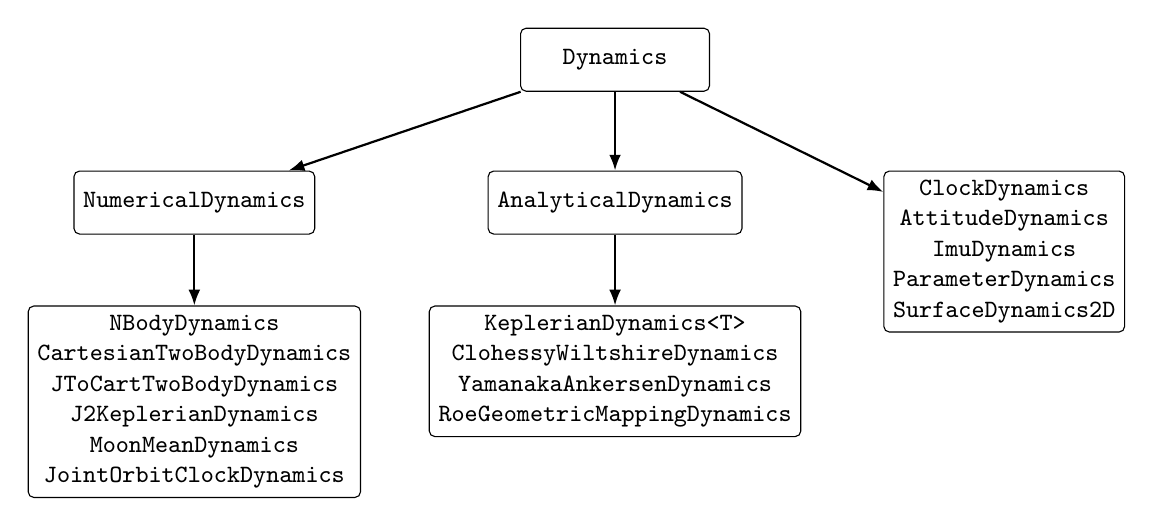
\begin{tikzpicture}[node distance=6mm and 8mm]
    \node[boxnode] (dyn) {\cpp{Dynamics}};
    \node[boxnode, below left=10mm and 26mm of dyn] (num) {\cpp{NumericalDynamics}};
    \node[boxnode, below=10mm of dyn] (ana) {\cpp{AnalyticalDynamics}};
    \node[boxnode, below right=10mm and 22mm of dyn] (oth)
      {\cpp{ClockDynamics}\\\cpp{AttitudeDynamics}\\\cpp{ImuDynamics}\\\cpp{ParameterDynamics}\\\cpp{SurfaceDynamics2D}};
    \node[boxnode, below=9mm of num] (nb)
      {\cpp{NBodyDynamics}\\\cpp{CartesianTwoBodyDynamics}\\\cpp{JToCartTwoBodyDynamics}\\\cpp{J2KeplerianDynamics}\\\cpp{MoonMeanDynamics}\\\cpp{JointOrbitClockDynamics}};
    \node[boxnode, below=9mm of ana] (kep)
      {\cpp{KeplerianDynamics<T>}\\\cpp{ClohessyWiltshireDynamics}\\\cpp{YamanakaAnkersenDynamics}\\\cpp{RoeGeometricMappingDynamics}};
    \draw[flow] (dyn) -- (num);
    \draw[flow] (dyn) -- (ana);
    \draw[flow] (dyn) -- (oth);
    \draw[flow] (num) -- (nb);
    \draw[flow] (ana) -- (kep);
  \end{tikzpicture}
  \caption{The dynamics class hierarchy. Arrows point from base to derived.}
  \label{fig:dyn-hierarchy}
\end{figure}

\begin{table}[H]
  \centering
  \caption{Concrete dynamics models and the state they propagate.}
  \label{tab:dyn-classes}
  \begin{tabularx}{\textwidth}{llL}
    \toprule
    Class & \cpp{GetStateType()} & Model \\
    \midrule
    \cpp{NBodyDynamics} & \code{Cart6} & \cref{eq:dyn-total}: harmonics, third bodies, SRP, drag, relativity \\
    \cpp{CartesianTwoBodyDynamics} & \code{Cart6} & \cref{eq:dyn-twobody} with constant $\mu$ \\
    \cpp{JToCartTwoBodyDynamics} & \code{Cart6} & two-body plus body-fixed $J_2$, \cref{eq:dyn-j2} \\
    \cpp{J2KeplerianDynamics} & \code{Cart6}$^{\dagger}$ & secular $J_2$ element rates, \cref{eq:dyn-j2-secular} \\
    \cpp{MoonMeanDynamics} & \code{Cart6}$^{\dagger}$ & lunar mean-element rates with Earth third-body terms \\
    \cpp{JointOrbitClockDynamics} & \code{JointOrbitClock} & $[\vec{r},\vec{v},b,d]$ or $[\vec{r},\vec{v},b,d,\dot{d}]$ \\
    \cpp{KeplerianDynamics<T>} & \code{T::TYPE} & advance the anomaly-like element by $n\,\Delta t$ \\
    \cpp{ClohessyWiltshireDynamics} & \code{RelCart6} & linearized relative motion, circular reference \\
    \cpp{YamanakaAnkersenDynamics} & \code{ClassicalOE} & eccentric-reference relative motion (STM only) \\
    \cpp{RoeGeometricMappingDynamics} & \code{QuasiNonsingROE} & ROE-to-RTN geometric mapping (matrix only) \\
    \bottomrule
  \end{tabularx}

  \vspace{2pt}
  {\small $^{\dagger}$ The state vector is in fact a set of classical elements;
  see the warning in \cref{sec:dyn-j2}.}
\end{table}

\subsection{The propagate interface}

Five overloads make up the contract. All of them take \emph{relative} simulation
times per \cref{eq:dyn-epoch}.

\begin{lstlisting}[language=cpp, caption={The \cpp{Dynamics} propagate interface.}, label={lst:dyn-interface}]
// cpp/lupnt/dynamics/dynamics.h :: Dynamics
virtual State Propagate(const State& x0, Real t0, Real tf, const State* u = nullptr) = 0;
virtual State Propagate(const State& x0, Real t0, Real tf, const State* u, MatXd* stm);
virtual MatX  Propagate(const State& x0, const VecX& tfs, const State* u = nullptr);
virtual State PropagateWithParams(const State& x0, Real t0, Real tf, const ParamState& params,
                                  const State* u = nullptr);
virtual State PropagateWithParams(const State& x0, Real t0, Real tf, const ParamState& params,
                                  const State* u, MatXd* stm_state, MatXd* stm_param);
virtual StateType GetStateType() const = 0;
\end{lstlisting}

The scalar overload is the only pure-virtual one; everything else has a default
implementation in \file{cpp/lupnt/dynamics/dynamics.cc}. The sequence overload
chains \cpp{Propagate} between consecutive entries of \code{tfs} and accumulates
each result as a row, optionally driving a progress bar;
\cpp{AnalyticalDynamics} overrides it to jump directly from \code{tfs(0)} to each
output epoch in an OpenMP-parallel loop, which analytic propagators can do
because they need no intermediate state.

\cpp{NumericalDynamics} additionally exposes \cpp{PropagateEx} and
\cpp{PropagateExStm}, which return a \cpp{TerminationInfo} describing whether the
integrator reached $t_f$ or stopped early (event trigger or iteration cap), the
time actually reached, and the number of steps taken. A truncated trajectory is
returned as the completed leading rows only.

\subsection{Bindings and configuration-driven construction}

\cpp{NBodyDynamics} is registered with the asset factory
(\code{REGISTER\_FACTORY\_CLASS(Dynamics, NBodyDynamics)}), so a YAML
\code{dynamics:} block naming it is enough to construct a fully configured force
model. When an agent declares no \code{dynamics:} block it inherits the shared
\code{world.force\_model}.

\section{State-transition matrix}
\label{sec:dyn-stm}

\subsection{Definition}

The state-transition matrix is the sensitivity of the propagated state to its
initial condition,

\begin{equation}
  \label{eq:dyn-stm}
  \mat{\Phi}(t_f,t_0) = \frac{\partial\vec{x}(t_f)}{\partial\vec{x}(t_0)},
\end{equation}

which for a smooth flow satisfies the variational equation

\begin{equation}
  \label{eq:dyn-variational}
  \dot{\mat{\Phi}} = \mat{A}(t)\,\mat{\Phi},
  \qquad
  \mat{A}(t) = \left.\frac{\partial f}{\partial\vec{x}}\right|_{\vec{x}(t)},
  \qquad
  \mat{\Phi}(t_0,t_0) = \mat{I}_{6} .
\end{equation}

Rows and columns follow the ordering of \cref{eq:dyn-state}. The composition and
inverse properties $\mat{\Phi}(t_2,t_0)=\mat{\Phi}(t_2,t_1)\mat{\Phi}(t_1,t_0)$
and $\mat{\Phi}(t_0,t_1)=\mat{\Phi}(t_1,t_0)^{-1}$ hold to integration accuracy
and are exercised by the filter tests.

\subsection{How it is obtained}

\lupnt{} does \emph{not} integrate \cref{eq:dyn-variational} as an augmented
$6+36$ state. Instead $\mat{\Phi}$ is obtained by forward-mode automatic
differentiation of the propagation itself: the whole integration --- ephemeris
lookups, frame rotations, the harmonic recursion, the shadow function --- is
carried out in the dual-number type \cpp{Real}, and the Jacobian of the map
$\vec{x}_0\mapsto\vec{x}_f$ is read off the tape. See \cref{chap:autodiff} for
the type system, the seeding strategy, and the parallel Jacobian driver.

\begin{lstlisting}[language=cpp, caption={The generic autodiff STM.}, label={lst:dyn-stm}]
// cpp/lupnt/dynamics/dynamics.cc :: Dynamics::Propagate
State Dynamics::Propagate(const State& x0, Real t0, Real tf, const State* u, MatXd* stm) {
  if (stm == nullptr) return Propagate(x0, t0, tf, u);
  auto func = [=, this](const VecX& x) {
    State xs = State(x, x0.GetNames(), x0.GetUnits());
    return Propagate(xs, t0, tf, u);
  };
  VecX xf_tmp;
  VecX x0_tmp = x0.cast<double>();
  jacobian(func, wrt(x0_tmp), at(x0_tmp), xf_tmp, *stm);
  State xf(xf_tmp, x0.GetNames(), x0.GetUnits());
  return xf;
}
\end{lstlisting}

For the $n$-body model the STM overload additionally requires that autodiff be
enabled, because with \code{autodiff: false} the harmonic field is evaluated in
plain \code{double} and the derivative information would be silently lost:

\begin{lstlisting}[language=cpp, caption={STM requires the autodiff path.}, label={lst:dyn-stm-check}]
// cpp/lupnt/dynamics/numerical_orbit_dynamics.cc :: NBodyDynamics::Propagate
State NBodyDynamics::Propagate(const State& x0, Real t0, Real tf, const State* u, MatXd* stm) {
  LUPNT_CHECK(use_ad_, "Autodiff not enabled", "NBodyDynamics");
  (void)u;
  return NumericalDynamics::Propagate(x0, t0, tf, u, stm);
}
\end{lstlisting}

The same mechanism yields the parameter sensitivity
$\partial\vec{x}_f/\partial\vec{p}$: \cpp{PropagateWithParams} differentiates the
propagation with respect to the \cpp{ParamState} vector, which is how the SRP and
drag ballistic coefficients become estimable states in the orbit-determination
filters.

\subsection{Analytic state-transition matrices}

The analytic propagators supply $\mat{\Phi}$ in closed form. For
\cpp{KeplerianDynamics<ClassicalOE>}, only the mean anomaly advances,
$M(t_f) = M(t_0) + n\,\Delta t$ with $n=\sqrt{\mu/a^3}$, so

\begin{equation}
  \label{eq:dyn-kep-stm}
  \mat{\Phi} = \mat{I}_{6} + \frac{\partial M(t_f)}{\partial a}\,
  \vec{e}_6\vec{e}_1\transpose,
  \qquad
  \frac{\partial M(t_f)}{\partial a} = -\frac{3}{2}\,\frac{n}{a}\,\Delta t ,
\end{equation}

with $\vec{e}_k$ the $k$-th unit vector; the $-3/2$ factor is the derivative of
$n\propto a^{-3/2}$. \cpp{ClohessyWiltshireDynamics} returns the classical
Clohessy--Wiltshire matrix
$\mat{\Phi} = \mat{A}\,\mat{B}(n\Delta t)$ built from the integration constants
solved for on the first call. STM computation is not implemented for the
\cpp{QuasiNonsingularOE} and \cpp{EquinoctialOE} specializations of
\cpp{KeplerianDynamics}, nor for \cpp{YamanakaAnkersenDynamics} and
\cpp{RoeGeometricMappingDynamics}: those overloads throw.

\section{Model boundaries}
\label{sec:dyn-boundaries}

This section states what the default configuration includes, what it
approximates, and what it omits.

\subsection{Defaults}

\begin{table}[H]
  \centering
  \caption{Defaults of a freshly constructed \cpp{NBodyDynamics}.}
  \label{tab:dyn-defaults}
  \begin{tabularx}{\textwidth}{llL}
    \toprule
    Setting & Default & Remark \\
    \midrule
    Integration frame & \code{MOON\_CI} & Moon-centred, ICRF-aligned axes \\
    Unit system & \code{SI\_UNITS} & \si{\meter}, \si{\second}, \si{\kilogram} \\
    Bodies & none & every body must be listed explicitly \\
    Relativity & \emph{enabled} & \cref{eq:dyn-moyer}, $\beta=\gamma=1$ \\
    SRP & disabled & enabled by \code{CR}/\code{area}/\code{mass} or \cpp{SetUseSrp} \\
    Drag & disabled & enabled by \code{CD}/\code{area}/\code{mass}; Earth only \\
    Autodiff & disabled & \code{double} field evaluation; no STM \\
    Solar irradiance & \SI{1361}{\watt\per\meter\squared} & $P_\odot = S_\odot/c$ \\
    Integrator & see \code{default\_integrator} & \code{RKF45} in the shipped configs \\
    Nominal step & \SI{10}{\second} & \code{dt} in the YAML block \\
    Degree/order & $0\times0$ (point mass) & shipped configs use $20\times20$ (truth) and $18\times18$ (filter) for the Moon \\
    \bottomrule
  \end{tabularx}
\end{table}

The shipped lunar scenarios (\file{configs/lunar_gnss_odts.yaml},
\file{configs/ephemeris.yaml}, \file{configs/ground_station_odts.yaml}) use a
Moon field of degree and order $20$, $8$, or $2$ depending on the study, with the
Earth and Sun as point masses, RKF45, and absolute/relative tolerances between
$10^{-6}$ and $10^{-12}$.

\subsection{What is approximated}

\begin{itemize}[leftmargin=1.4em]
  \item \textbf{Gravity field truncation.} The field is truncated at the
    configured $(n,m)$. Truncating the lunar field at degree $20$ leaves the
    residual acceleration of the omitted degrees, which for a
    \SI{100}{\kilo\meter} circular lunar orbit is the dominant remaining error
    source; the truncation degree, not the integrator tolerance, sets the
    achievable propagation accuracy. Increasing the degree costs
    $O(n_\mathrm{max}^2)$ per evaluation.
  \item \textbf{Point-mass third bodies.} Earth and Sun enter through
    \cref{eq:dyn-pointmass} only; the Earth's oblateness is never seen by a lunar
    orbiter in this model. Solid-body and ocean tides, and the associated
    time-varying Stokes coefficients, are not modelled for any body.
  \item \textbf{Cannonball SRP.} \Cref{eq:dyn-srp} assumes a spherical spacecraft
    with a single scalar $C_R$: no attitude dependence, no panel model, no
    thermal re-radiation, and no albedo or infrared radiation from the central
    body. Occulting bodies are treated as spheres of radius \code{body.R}, so
    the shadow geometry ignores oblateness, terrain, and atmospheric refraction
    at the terminator.
  \item \textbf{Fixed exponent Harris--Priester.} The density model fixes
    $n_p=3$ rather than selecting $2$ or $6$ by inclination, uses a low-precision
    solar ephemeris for the bulge apex, and has no solar-activity ($F_{10.7}$,
    $A_p$) dependence at all: the min/max table is static.
  \item \textbf{Relativity.} \Cref{eq:dyn-moyer} keeps terms to $O(c^{-2})$ and
    uses Newtonian body accelerations in the $\ddot{\vec{r}}_j$ terms. It is
    evaluated over the \emph{configured} bodies only, so the correction changes
    if bodies are added or removed for reasons unrelated to relativity.
  \item \textbf{Autodiff clamping.} \cpp{ClampUnit} and the $y^2$ floor
    (\cref{sec:dyn-srp}) perturb the shadow function by less than $10^{-9}$ in
    value in exchange for a finite derivative. Near a grazing shadow boundary the
    resulting $\mat{\Phi}$ is a smoothed approximation of a genuinely
    non-differentiable map.
\end{itemize}

\subsection{What is omitted}

\begin{itemize}[leftmargin=1.4em]
  \item Frame-dragging (Lense--Thirring) and geodesic precession.
  \item Empirical accelerations, manoeuvre and thrust models in the orbit
    right-hand side; a control input \code{u} is accepted by the interface but
    ignored by every orbit model.
  \item Drag for any body other than the Earth, and any thermospheric model other
    than Harris--Priester.
  \item Albedo and planetary infrared radiation pressure.
  \item Process noise: the dynamics are deterministic. Stochastic terms are
    supplied by the filters, not by the dynamics models.
\end{itemize}

\subsection{Structural constraints}

\begin{itemize}[leftmargin=1.4em]
  \item \cpp{SetUnits} must be called \emph{before} \cpp{AddBody}: it aborts if
    any body is already registered, and \cpp{AddBody} rejects a body whose
    \code{units} differ from the model's.
  \item \cpp{ComputeRates} aborts if \code{frame\_} is \code{UNDEFINED}.
  \item \cpp{JToCartTwoBodyDynamics} requires the integration and body-fixed
    frames to share an origin.
  \item A body may be added only once; \cpp{AddBody} aborts on a duplicate
    \code{BodyId}.
  \item The STM overload of \cpp{NBodyDynamics::Propagate} aborts unless
    \code{autodiff: true}.
\end{itemize}

\subsection{Validation}

Cross-validation drivers compare the propagated trajectory against GMAT
\citep{gmat2023} (\file{cpp/test/gmat/test_orbit_dynamics_gmat.cc}) and
Orekit (\file{cpp/test/orekit/test_orbit_dynamics_orekit.cc}). The Earth
point-mass-plus-$J_2$ case agrees to a few hundred metres in position and
\SI{0.15}{\meter\per\second} in velocity over the compared arc, the residual
being dominated by the differing $J_2$ conventions rather than by the integrator.
The pure two-body and $J_2$ element-rate models are additionally checked against
their closed-form solutions, and the relativistic $n$-body term against
\cref{eq:dyn-schwarzschild}. The accuracy actually achieved in the lunar
orbit-determination scenarios, and its sensitivity to the truncation degree, is
reported in \citep[Ch.~2]{iiyama2026thesis}.

\chapter{Numerical Integration}
\label{chap:integration}

This chapter specifies the mathematical contract of \lupnt{}'s ordinary
differential equation (ODE) integrators: the family of explicit Runge--Kutta
methods they realise, the Butcher tableaux they carry, the embedded error
estimates and step-size control laws of the adaptive members, the termination
semantics of a propagation run, and the way the state-transition (sensitivity)
matrix is carried through the integration by the differentiable scalar type of
\cref{chap:autodiff}. Everything here is implemented by
\file{cpp/lupnt/numerics/integrator.h} and
\file{cpp/lupnt/numerics/integrator.cc}; the sensitivity machinery lives in
\file{cpp/lupnt/numerics/math_utils.cc}, and the callers are the numerical
dynamics models of \cref{chap:dynamics}. The reference for the general theory,
the order conditions, and the step-size controller is the standard treatment
of nonstiff initial value problems \citep{hairer1993}; the individual embedded
pairs follow \citep{fehlberg1969} and \citep{dormand1980}.

The chapter is written as a specification rather than a description: the
equations below are the contract that a regression test may assert against.
Three of those contracts were, for a time, violated by the implementation: one
coefficient of the \cpp{RK8} tableau, the stage times of \cpp{PD45}, and the
acceptance threshold of the \cpp{IRKF} controller. All three have been
corrected, and all three are now pinned by
\file{cpp/test/numerics/test_integrator_order.cc}. Each is recorded below, in
the past tense, next to the method it affected rather than in a defect list:
how each one hid --- one behind a weak tolerance, one behind an autonomous
test problem, one behind an integer division --- is the more useful half of
the story. \Cref{sec:int-boundaries} is reserved for what is still a genuine
limitation.

\section{ODE and State Contract}
\label{sec:int-contract}

Every integrator advances a first-order, explicitly time-dependent system
\begin{equation}
  \label{eq:int-ode}
  \dot{x} = f(t, x),
  \qquad x \in \mathbb{R}^{n},
  \qquad f : \mathbb{R}\times\mathbb{R}^{n} \to \mathbb{R}^{n},
\end{equation}
from an initial time $t_0$ to a final time $t_f$. The independent variable $t$
is in seconds; the step size $h$ carries the sign of the propagation
direction. The right-hand side is the \cpp{ODE} type,

\begin{lstlisting}[language=cpp, caption={Right-hand side type. Source: \code{cpp/lupnt/numerics/integrator.h}}, label={lst:int-ode}]
// cpp/lupnt/numerics/integrator.h :: ODE
using ODE = std::function<VecX(Real, const State&)>;
\end{lstlisting}

Two properties of \cref{lst:int-ode} are contractual and used throughout the
rest of this chapter.

\begin{enumerate}[leftmargin=1.5cm]
  \item The scalar is \cpp{Real}, not \cpp{double}. Both the time argument and
    every component of the returned rate vector are forward-mode dual numbers
    (\cref{sec:ad-real}). This is what allows an entire propagation to be
    differentiated with respect to its initial condition without writing a
    variational equation --- see \cref{sec:int-stm}.
  \item The integrator does not interpret the contents of the state. Units,
    reference frame, epoch offset, and the ordering of the components are
    entirely the property of the calling dynamics model
    (\cref{chap:dynamics}). \cpp{NumericalOrbitDynamics},
    \cpp{ClockDynamics}, and \cpp{JointOrbitClockDynamics} each build an
    \cpp{ODE} from their own force and derivative models and hand it to
    \cpp{Integrator::Propagate}.
\end{enumerate}

\begin{lupntnote}
  Because the \cpp{ODE} closure is captured by the numerical dynamics model,
  the absolute epoch enters through the global reference epoch: a dynamics
  model evaluates its ephemeris at $t_{\TDB} = t_{\mathrm{epoch}} + t$, where
  $t$ is the integrator's independent variable. The integrator itself is
  epoch-agnostic.
\end{lupntnote}

\section{Integrator Selection and Configuration}
\label{sec:int-selection}

The concrete method is chosen by the enumeration
\begin{equation}
  \label{eq:int-types}
  \texttt{IntegratorType} \in
  \{\ \texttt{RK4},\ \texttt{RK8},\ \texttt{RKF45},\ \texttt{PD45}\ \},
\end{equation}
with \code{RK4} the default (\cpp{default\_integrator} in
\file{cpp/lupnt/numerics/integrator.h}). \code{RK4} and \code{RK8} are
fixed-step; \code{RKF45} and \code{PD45} carry embedded error estimates and
adapt their internal step.

\begin{lstlisting}[language=cpp, caption={Integrator instantiation. Source: \code{cpp/lupnt/dynamics/numerical\_orbit\_dynamics.cc}}, label={lst:int-select}]
// cpp/lupnt/dynamics/numerical_orbit_dynamics.cc :: NumericalDynamics::SetIntegrator
void NumericalDynamics::SetIntegrator(IntegratorType integ) {
  if (integ == IntegratorType::RK4) {
    integrator_ = MakeUnique<RK4>();
  } else if (integ == IntegratorType::RK8) {
    integrator_ = MakeUnique<RK8>();
  } else if (integ == IntegratorType::RKF45) {
    integrator_ = MakeUnique<RKF45>();
  } else if (integ == IntegratorType::PD45) {
    integrator_ = MakeUnique<PD45>();
  } else {
    LUPNT_CHECK(false, "Invalid Integrator Type", "NumericalOrbitDynamics");
  }
}
\end{lstlisting}

The configuration knobs a scenario file may set are listed in
\cref{tab:int-knobs}. They are read once, in the
\cpp{NumericalDynamics(Config\&)} constructor; the tolerance block is applied
only if at least one of its three keys is present, so the built-in defaults
survive a partial configuration.

\begin{table}[H]
  \centering
  \caption{Integration configuration keys, read by
    \cpp{NumericalDynamics(Config\&)} in
    \code{cpp/lupnt/dynamics/numerical\_orbit\_dynamics.cc} and validated by
    \cpp{IntegratorParams::CheckIntegratorParams}.}
  \label{tab:int-knobs}
  \begin{tabularx}{\textwidth}{llL}
    \toprule
    Key & Default & Meaning \\
    \midrule
    \code{integrator} & \code{RK4} & One of \cref{eq:int-types}, parsed by
      name through \code{magic\_enum}. \\
    \code{dt}         & --- & Nominal step size $\mathrm{d}t$ in seconds; must
      be positive. For the fixed-step methods this is the step; for the
      adaptive methods it is the outer marching increment
      (\cref{sec:int-loop}). \\
    \code{max\_iter}  & \num{20} & Maximum number of rejected attempts an
      adaptive \cpp{Step} may make before throwing. Must be $>0$. \\
    \code{abstol}     & \num{1e-6} & Absolute tolerance $\eta_a$. Must be
      $>0$. \\
    \code{reltol}     & \num{1e-6} & Relative tolerance $\eta_r$. Must be
      $>0$. \\
    \bottomrule
  \end{tabularx}
\end{table}

\begin{lstlisting}[language=yamlcfg, caption={Scenario-file form of \cref{tab:int-knobs}.}, label={lst:int-yaml}]
dynamics:
  integrator: RKF45   # RK4 | RK8 | RKF45 | PD45
  dt: 60.0            # [s]
  abstol: 1.0e-9
  reltol: 1.0e-9
  max_iter: 30
\end{lstlisting}

\section{The Fixed-Step Explicit Runge--Kutta Contract}
\label{sec:int-rk}

An explicit $s$-stage Runge--Kutta method is defined by a Butcher tableau
$(a_{ij}, b_i, c_i)$ with $a_{ij} = 0$ for $j \ge i$,
\begin{equation}
  \label{eq:int-tableau}
  \renewcommand{\arraystretch}{1.15}
  \begin{array}{c|cccc}
    c_1    &        &        &        &           \\
    c_2    & a_{21} &        &        &           \\
    \vdots & \vdots & \ddots &        &           \\
    c_s    & a_{s1} & a_{s2} & \cdots & a_{s,s-1} \\
    \hline
           & b_1    & b_2    & \cdots & b_s
  \end{array}
\end{equation}
which advances the solution over one step of size $h$ by
\begin{align}
  \label{eq:int-stage}
  k_i &= f\!\left(t + c_i h,\ x_k + \sum_{j<i} a_{ij}\, k_j\right),
        \qquad i = 1,\dots,s, \\
  \label{eq:int-update}
  x_{k+1} &= x_k + h \sum_{i=1}^{s} b_i\, k_i .
\end{align}

Two structural conditions are used repeatedly below as verification checks
\citep[Ch.~II.1]{hairer1993}:
\begin{equation}
  \label{eq:int-consistency}
  \sum_{i=1}^{s} b_i = 1
  \qquad\text{(consistency)},
  \qquad\qquad
  c_i = \sum_{j<i} a_{ij}
  \qquad\text{(row-sum / node condition)}.
\end{equation}
The row-sum condition is what makes the stage evaluation time $t + c_i h$
consistent with the stage argument; a tableau that violates it integrates
autonomous systems at full order but loses order on any explicitly
time-dependent right-hand side. Both of the tableau defects \lupnt{} once
carried --- \cref{sec:int-rk8} and \cref{sec:int-pd45} --- were of exactly
this kind, and \cref{eq:int-consistency} is what diagnosed them. It is now
asserted directly, as a property of the coefficient arrays rather than of a
propagated trajectory, by the cases
\code{numerics.integrator\_order.rk8\_tableau\_consistency} and
\code{numerics.integrator\_order.pd45\_node\_consistency} in
\file{cpp/test/numerics/test_integrator_order.cc}.

\begin{lupntnote}
  In the \lupnt{} source the stage derivatives are stored \emph{pre-scaled} by
  the step, $k_i \leftarrow h\, f(\cdot)$ (written \code{f(...) * dt}), so the
  implemented update reads $x_{k+1} = x_k + \sum_i b_i k_i$ without the outer
  $h$. Every tableau in this chapter is stated in the unscaled convention of
  \cref{eq:int-stage}--\cref{eq:int-update}; the two agree because the scaling
  is uniform across stages.
\end{lupntnote}

\subsection{RK4: the classical fourth-order method}
\label{sec:int-rk4}

\cpp{RK4} implements the classical tableau
\begin{equation}
  \label{eq:int-rk4-tableau}
  \renewcommand{\arraystretch}{1.3}
  \begin{array}{c|cccc}
    0            &             &             &             &             \\
    \tfrac{1}{2} & \tfrac{1}{2}&             &             &             \\
    \tfrac{1}{2} & 0           & \tfrac{1}{2}&             &             \\
    1            & 0           & 0           & 1           &             \\
    \hline
                 & \tfrac{1}{6}& \tfrac{1}{3}& \tfrac{1}{3}& \tfrac{1}{6}
  \end{array}
\end{equation}
which satisfies both conditions of \cref{eq:int-consistency} and expands to
\begin{align}
  \label{eq:int-rk4-stages}
  k_1 &= f(t, x_k), &
  k_2 &= f\!\left(t+\tfrac{h}{2},\ x_k + \tfrac{h}{2}k_1\right), \nonumber \\
  k_3 &= f\!\left(t+\tfrac{h}{2},\ x_k + \tfrac{h}{2}k_2\right), &
  k_4 &= f\!\left(t+h,\ x_k + h\,k_3\right),
\end{align}
\begin{equation}
  \label{eq:int-rk4-update}
  x_{k+1} = x_k + \frac{h}{6}\left(k_1 + 2k_2 + 2k_3 + k_4\right).
\end{equation}
The method is of order $4$ with a local truncation error $O(h^5)$, and it is
exact for any right-hand side that is a polynomial of degree $\le 3$ in $t$
alone.

\begin{lstlisting}[language=cpp, caption={Classical RK4 step. Source: \code{cpp/lupnt/numerics/integrator.cc}}, label={lst:int-rk4}]
// cpp/lupnt/numerics/integrator.cc :: RK4::Step
State RK4::Step(const ODE& f, Real t, const State& x, Real dt) {
  State k_1 = f(t, x) * dt;

  Real  t1  = t + dt / 2.0;
  State x1  = x + k_1 / 2.0;
  State k_2 = f(t1, x1) * dt;

  Real  t2  = t + dt / 2.0;
  State x2  = x + k_2 / 2.0;
  State k_3 = f(t2, x2) * dt;

  Real  t3  = t + dt;
  State x3  = x + k_3;
  State k_4 = f(t3, x3) * dt;

  State dx = (k_1 + k_2 * 2.0 + k_3 * 2.0 + k_4) / 6.0;
  return x + dx;
}
\end{lstlisting}

\subsection{RK8: the ten-stage, seventh-order method}
\label{sec:int-rk8}

\cpp{RK8} is a ten-stage explicit method of the Shanks/Cooper--Verner family.
Its order is $7$, not $8$: the name overstates it, and
\cref{sec:int-rk8-order} shows that this is a consequence of the stage count
rather than a residual defect.
Its coefficient matrix is dense enough that reproducing $a_{ij}$ as a
$10\times 9$ array is unreadable at this page width; the tableau is therefore
given in the row-factored form in which the source writes it
(\cref{tab:int-rk8}), from which the individual $a_{ij}$ follow by
distributing the common denominator. The stage nodes are
\begin{equation}
  \label{eq:int-rk8-nodes}
  c = \left[\,0,\ \tfrac{4}{27},\ \tfrac{2}{9},\ \tfrac{1}{3},\ \tfrac{1}{2},
      \ \tfrac{2}{3},\ \tfrac{1}{6},\ 1,\ \tfrac{5}{6},\ 1\,\right],
\end{equation}
and the final combination uses only seven of the ten stages,
\begin{equation}
  \label{eq:int-rk8-update}
  x_{k+1} = x_k + \frac{h}{840}\Big(
    41 k_1 + 27 k_4 + 272 k_5 + 27 k_6 + 216 k_7 + 216 k_9 + 41 k_{10}
  \Big),
\end{equation}
whose weights sum to $840/840 = 1$, satisfying consistency.

\begin{table}[H]
  \centering
  \caption{Stage arguments of \cpp{RK8::Step}, exactly as coded in
    \code{cpp/lupnt/numerics/integrator.cc}. Stage $i$ evaluates
    $k_i = h f(t + c_i h,\ X_i)$. The last column is
    $\sum_{j<i} a_{ij}$, which must equal $c_i$ by
    \cref{eq:int-consistency}.}
  \label{tab:int-rk8}
  \setlength{\tabcolsep}{4pt}
  \begin{tabular}{clll}
    \toprule
    $i$ & $c_i$ & Stage argument $X_i$ & $\sum_j a_{ij}$ \\
    \midrule
    $1$  & $0$            & $x_k$ & $0$ \\
    $2$  & $\tfrac{4}{27}$& $x_k + \tfrac{4}{27}k_1$ & $\tfrac{4}{27}$ \\
    $3$  & $\tfrac{2}{9}$ & $x_k + \tfrac{1}{18}\left(k_1 + 3k_2\right)$
         & $\tfrac{2}{9}$ \\
    $4$  & $\tfrac{1}{3}$ & $x_k + \tfrac{1}{12}\left(k_1 + 3k_3\right)$
         & $\tfrac{1}{3}$ \\
    $5$  & $\tfrac{1}{2}$ & $x_k + \tfrac{1}{8}\left(k_1 + 3k_4\right)$
         & $\tfrac{1}{2}$ \\
    $6$  & $\tfrac{2}{3}$
         & $x_k + \tfrac{1}{54}\left(13k_1 - 27k_3 + 42k_4 + 8k_5\right)$
         & $\tfrac{2}{3}$ \\
    $7$  & $\tfrac{1}{6}$
         & $x_k + \tfrac{1}{4320}\left(389k_1 - 54k_3 + 966k_4 - 824k_5
           + 243k_6\right)$
         & $\tfrac{1}{6}$ \\
    $8$  & $1$
         & $x_k + \tfrac{1}{20}\left(-231\,k_1 + 81k_3 - 1164k_4
           + 656k_5 - 122k_6 + 800k_7\right)$
         & $1$ \\
    $9$  & $\tfrac{5}{6}$
         & $x_k + \tfrac{1}{288}\left(-127k_1 + 18k_3 - 678k_4 + 456k_5
           - 9k_6 + 576k_7 + 4k_8\right)$
         & $\tfrac{5}{6}$ \\
    $10$ & $1$
         & $x_k + \tfrac{1}{820}\left(1481k_1 - 81k_3 + 7104k_4 - 3376k_5
           + 72k_6 - 5040k_7 - 60k_8 + 720k_9\right)$
         & $1$ \\
    \bottomrule
  \end{tabular}
\end{table}

Every row of \cref{tab:int-rk8} now satisfies the node condition, and the
weights of \cref{eq:int-rk8-update} sum to $1$; the tableau as coded is
consistent throughout.

\begin{lstlisting}[language=cpp, caption={Final combination of the ten-stage method. Source: \code{cpp/lupnt/numerics/integrator.cc}}, label={lst:int-rk8}]
// cpp/lupnt/numerics/integrator.cc :: RK8::Step (stages 8 and 10, and the combination)
// 8
// The leading coefficient is -231, not -234: the row must sum to c_8 = 1
// (the consistency condition c_i = sum_j a_ij), and
// (-231 + 81 - 1164 + 656 - 122 + 800)/20 = 1 exactly, whereas -234 gives
// 17/20 and silently drops the method to 3rd order. See
// cpp/test/numerics/test_integrator_order.cc.
Real t7 = t + dt;
State x7
    = x + (1.0 / 20) * (-231 * k_1 + 81 * k_3 - 1164 * k_4 + 656 * k_5 - 122 * k_6 + 800 * k_7);
State k_8 = f(t7, x7) * dt;
// ...
State dx
    = (41 * k_1 + 27 * k_4 + 272 * k_5 + 27 * k_6 + 216 * k_7 + 216 * k_9 + 41 * k_10) / 840;
return x + dx;
\end{lstlisting}

\subsection{Order of RK8: the stage-8 coefficient, and Butcher's barrier}
\label{sec:int-rk8-order}

\paragraph{The corrected coefficient.}
\label{warn:int-rk8}
Stage $8$ was for a long time coded with $-234$ in place of the $-231$ of
\cref{tab:int-rk8}, and was the only row of the tableau that failed the node
condition of \cref{eq:int-consistency}: its coefficients summed to
$17/20 = 0.85$ against a node of $c_8 = 1$. With $-231$ the row sums to
$20/20 = 1$ exactly. Every other row, and the weight vector
\cref{eq:int-rk8-update}, already satisfied the conditions, which is what
identified the entry as an isolated transcription error rather than a
different tableau. Nor is $-231$ merely \emph{a} value that restores the row
sum: repairing any other single coefficient of the row instead --- there are
five candidates --- gives a method that measures order $4$. The intended
coefficient is therefore uniquely determined by the row it sits in.

\paragraph{What the defect cost, and how it hid.}
Let $e(h)$ be the global error at $t = 1$ of a propagation over $t\in[0,1]$
and let
\begin{equation}
  \label{eq:int-emporder}
  p_{\mathrm{emp}} = \log_2 \frac{e(h)}{e(h/2)}
\end{equation}
be the empirical order. Measured with the production \cpp{Real} class at
$h = 1/4$, the as-coded method returned $p_{\mathrm{emp}} = 3.18$ on
$\dot y = -y$ and $2.83$ on the non-autonomous $\dot y = y\cos t$ --- an
order-$3$ method wearing an order-$8$ name. With $-231$ the same experiment
gives $p_{\mathrm{emp}} > 8$ on $\dot y = -y$ and $6.95$ on
$\dot y = y\cos t$. The first of those two figures is not evidence of order
$8$: on a linear, constant-coefficient problem the whole step collapses to a
polynomial in $h\lambda$ that happens to reproduce $e^{h\lambda}$ to higher
degree than the general order conditions require, so such a problem
superconverges and cannot be used to measure order at all. The honest
measurement is the local truncation error evaluated in exact rational
arithmetic on $\dot y = y^{2}$ and $\dot y = t\,y^{2}$: at four successively
halved step sizes it decays as $h^{p+1}$ with $p+1 = 8.00$, $8.13$, $8.02$
and $8.00$, i.e.\ a local error of $O(h^{8})$ and hence a global order of
$7$.

The reason the defect survived for so long is that the unit test in
\file{cpp/test/numerics/test_integrator_extra.cc} propagates with
$\mathrm{d}t = \num{1e-3}$ against a tolerance of \num{1e-8}. An order-$3$
method clears that comfortably; only a test that varies $h$ and looks at the
\emph{ratio} of errors can see the difference. That is what
\code{numerics.integrator\_order.rk8\_is\_seventh\_order} and
\code{numerics.integrator\_order.rk8\_tableau\_consistency}, in
\file{cpp/test/numerics/test_integrator_order.cc}, now do.

\paragraph{Order 7 is optimal for ten stages.}
The remaining gap between the name and the method is not a defect and cannot
be closed by a better tableau. Butcher's order barrier for explicit
Runge--Kutta methods states that order $8$ requires at least $s = 11$ stages
\citep[Thm.~II.5.1]{hairer1993}; \cpp{RK8} has $s = 10$, so order $8$ is
unattainable for it by construction, and order $7$ --- which needs $s \ge 9$
--- is the best a ten-stage explicit method can do. The corrected tableau
attains that bound. It is the class name, not the coefficients, that is
wrong.

Renaming is nonetheless not a free change and should not be made silently:
\code{IntegratorType::RK8} is public API, is selected by name through
\code{magic\_enum} from the \code{integrator} key of \cref{tab:int-knobs},
and is re-exported in the Python bindings, so every scenario file and every
\pylupnt{} script that names it would break. Until a deprecation path is
provided, the name is documented as a misnomer rather than corrected: see
\cref{sec:int-boundaries}.

\section{Embedded Pairs and the Local Error Estimate}
\label{sec:int-embedded}

An embedded pair augments \cref{eq:int-tableau} with a second weight vector
$b^{*}$ of one order lower (or higher) sharing the same stages
$k_1,\dots,k_s$. Evaluating both weightings costs nothing beyond the stages
already computed and yields two approximations at $t+h$,
\begin{equation}
  \label{eq:int-pair}
  \hat{x}^{\mathrm{high}}_{k+1} = x_k + h\sum_{i=1}^{s} b_i k_i,
  \qquad
  \hat{x}^{\mathrm{low}}_{k+1}  = x_k + h\sum_{i=1}^{s} b^{*}_i k_i,
\end{equation}
whose difference estimates the local truncation error of the lower-order
member componentwise,
\begin{equation}
  \label{eq:int-err}
  e_i = \left| \hat{x}^{\mathrm{high}}_{k+1,i}
             - \hat{x}^{\mathrm{low}}_{k+1,i} \right|,
  \qquad i = 1,\dots,n .
\end{equation}
\lupnt{} contains two embedded pairs with two \emph{different} controllers:
\cpp{RKF45}, which derives from the abstract base \cpp{IRKF} and uses the
componentwise controller of \cref{sec:int-control}, and \cpp{PD45}, which is
self-contained and uses the root-mean-square controller of
\cref{sec:int-pd45}.

\subsection{The \texorpdfstring{\cpp{IRKF}}{IRKF} controller}
\label{sec:int-control}

\cpp{IRKF} scales \cref{eq:int-err} by a mixed absolute/relative tolerance
built from the \emph{high}-order solution,
\begin{equation}
  \label{eq:int-tol}
  \mathrm{tol}_i = \max\!\left(
    \eta_r \left|\hat{x}^{\mathrm{high}}_{k+1,i}\right|,\ \eta_a
  \right),
  \qquad
  \varepsilon = \max_{i} \frac{e_i}{\mathrm{tol}_i},
\end{equation}
with $\eta_r = \code{reltol}$ and $\eta_a = \code{abstol}$ from
\cref{tab:int-knobs}. The step is accepted when every component satisfies
\begin{equation}
  \label{eq:int-accept}
  \frac{e_i}{\mathrm{tol}_i} \le \theta,
  \qquad
  \theta = (p+1)^{\,(p+1)/p},
\end{equation}
where $p$ is the order of the lower-order member ($p = 4$ for \cpp{RKF45}).
\Cref{eq:int-accept} is the non-conservative acceptance threshold of the
standard step-size-control literature \citep[Ch.~II.4]{hairer1993}; for $p=4$ its exact value is
$5^{1.25} \approx 7.48$. Whether the step is accepted or not, the step size is
rescaled by
\begin{equation}
  \label{eq:int-scale}
  s = \beta\,\varepsilon^{-1/(p+1)},
  \qquad
  s \leftarrow \min\big(2,\ \max(0.5,\ s)\big),
  \qquad
  \mathrm{d}t \leftarrow s\,\mathrm{d}t,
\end{equation}
with safety factor $\beta = 0.9$ and the clamp restricting any single
adjustment to a factor of two in either direction. The exponent $-1/(p+1)$
follows from $e \sim C h^{p+1}$: to bring a measured $\varepsilon$ down to $1$
the step must be scaled by $\varepsilon^{-1/(p+1)}$, and $\beta$ absorbs the
error in that extrapolation.

\begin{lstlisting}[language=cpp, caption={Componentwise error test and step-size controller. Source: \code{cpp/lupnt/numerics/integrator.cc}}, label={lst:int-relerr}]
// cpp/lupnt/numerics/integrator.cc :: IRKF::ComputeRelError
bool IRKF::ComputeRelError(const State& x_new_low, const State& x_new_high, Real& dt) {
  double tol = 0.0;
  double error = 0.0;
  bool within_tolerance = true;
  double max_error = 0.0;

  // Non-conservative acceptance threshold. J.C. Butcher, Numerical Methods
  // for Ordinary Differential Equations, p291.
  //
  // The exponent must be evaluated in floating point: `order_` is an int, so
  // `(order_ + 1) / order_` is integer division and collapses to 1 for every
  // order >= 1, giving 5 instead of 5^1.25 ~ 7.48 for RKF45.
  double accept_thresh
      = std::pow(order_ + 1, static_cast<double>(order_ + 1) / static_cast<double>(order_));

  for (size_t i = 0; i < x_new_low.size(); ++i) {
    error = abs(x_new_high(i) - x_new_low(i));
    tol = max(params_.reltol * abs(x_new_high(i)), params_.abstol);
    max_error = std::max(max_error, error / tol);
    if ((error / tol) > accept_thresh) within_tolerance = false;
  }

  // Update timestep
  double beta = 0.9;  // safety factor
  double s = beta * std::pow(1.0 / max_error, 1.0 / (order_ + 1));
  s = std::max(0.5, std::min(2.0, s));  // J.C. Butcher, Numerical Methods for
                                        // Ordinary Differential Equations, (371a)
  dt = s * dt;

  return within_tolerance;
}
\end{lstlisting}

\begin{lupntnote}
  \label{warn:int-thresh}
  The two \code{static\_cast<double>} in \cref{lst:int-relerr} are load-bearing
  and were not always there. \cpp{order\_} is an \cpp{int}, so the exponent
  \code{(order\_ + 1) / order\_} was previously evaluated in \emph{integer}
  arithmetic; for \cpp{RKF45} that is $5/4 = 1$, not $1.25$, and in fact the
  quotient collapses to $1$ for \emph{every} order $p \ge 1$, so the
  order-dependence of \cref{eq:int-accept} vanished entirely. The realised
  threshold was $\theta = 5^{1} = 5$ instead of $5^{1.25} \approx 7.48$: a
  third tighter than intended, and therefore conservative rather than wrong
  --- it never accepted a step the published law would have rejected. What it
  did do is silently stop matching the reference the source cites for it
  (Butcher, \emph{Numerical Methods for Ordinary Differential Equations},
  p.~291), which is exactly the kind of drift a specification is meant to
  catch. The threshold now evaluates to $5^{1.25}$ for \cpp{RKF45} and to
  $(p+1)^{(p+1)/p}$ in general.
\end{lupntnote}

The retry loop wrapping the controller is \cpp{IRKF::Step}. It calls the
subclass \cpp{Update} to form the pair, tests it, and repeats with the
rescaled step, up to \code{max\_iter} attempts; on exhaustion it throws
through \code{LUPNT\_CHECK}. Note that the value returned is the
\emph{low}-order member: \lupnt{} does not perform local extrapolation, so the
achieved order of \cpp{RKF45} is $4$ and the fifth-order solution serves only
as the error yardstick.

\begin{lstlisting}[language=cpp, caption={Adaptive retry loop. Source: \code{cpp/lupnt/numerics/integrator.cc}}, label={lst:int-irkf-step}]
// cpp/lupnt/numerics/integrator.cc :: IRKF::Step
State IRKF::Step(const ODE& f, Real t, const State& x, Real dt) {
  int n = x.size();
  State x_new_low(n), x_new_high(n);

  int iter;
  for (iter = 0; iter < params_.max_iter; ++iter) {
    Update(f, t, x, dt, x_new_low, x_new_high);
    bool within_tolerance = ComputeRelError(x_new_low, x_new_high, dt);
    if (within_tolerance) break;
  }
  LUPNT_CHECK(iter < params_.max_iter,
              "IRKF did not converge, increase max_iter or reduce tolerance", "IRKF");

  return x_new_low;
}
\end{lstlisting}

\subsection{RKF45: the Fehlberg 4(5) pair}
\label{sec:int-rkf45}

\cpp{RKF45} is the six-stage Fehlberg pair \citep{fehlberg1969}, constructed
as \cpp{IRKF(4)}. Its tableau, with the fifth-order weights $b$ on the first
rule line and the fourth-order weights $b^{*}$ on the second, is

\begin{equation}
  \label{eq:int-rkf45-tableau}
  {\setlength{\arraycolsep}{3pt}
  \renewcommand{\arraystretch}{1.35}
  \begin{array}{c|cccccc}
    0 & & & & & & \\
    \tfrac{1}{4}    & \tfrac{1}{4} & & & & & \\
    \tfrac{3}{8}    & \tfrac{3}{32} & \tfrac{9}{32} & & & & \\
    \tfrac{12}{13}  & \tfrac{1932}{2197} & -\tfrac{7200}{2197}
                    & \tfrac{7296}{2197} & & & \\
    1               & \tfrac{439}{216} & -8 & \tfrac{3680}{513}
                    & -\tfrac{845}{4104} & & \\
    \tfrac{1}{2}    & -\tfrac{8}{27} & 2 & -\tfrac{3544}{2565}
                    & \tfrac{1859}{4104} & -\tfrac{11}{40} & \\
    \hline
    b               & \tfrac{16}{135} & 0 & \tfrac{6656}{12825}
                    & \tfrac{28561}{56430} & -\tfrac{9}{50} & \tfrac{2}{55} \\
    b^{*}           & \tfrac{25}{216} & 0 & \tfrac{1408}{2565}
                    & \tfrac{2197}{4104} & -\tfrac{1}{5} & 0
  \end{array}}
\end{equation}

Both weight vectors sum to $1$ and every row satisfies the node condition of
\cref{eq:int-consistency}, so the implemented tableau is correct as published.
Written out, the pair is
\begin{align}
  \label{eq:int-rkf45-low}
  \hat{x}^{\mathrm{low}}_{k+1}
    &= x_k + \tfrac{25}{216}k_1 + \tfrac{1408}{2565}k_3
       + \tfrac{2197}{4104}k_4 - \tfrac{1}{5}k_5, \\
  \label{eq:int-rkf45-high}
  \hat{x}^{\mathrm{high}}_{k+1}
    &= x_k + \tfrac{16}{135}k_1 + \tfrac{6656}{12825}k_3
       + \tfrac{28561}{56430}k_4 - \tfrac{9}{50}k_5 + \tfrac{2}{55}k_6,
\end{align}
with $h$-scaled stages as noted in \cref{sec:int-rk}. Stage $k_2$ contributes
to neither weighting; it exists only to build $k_3$ onwards.

\begin{lstlisting}[language=cpp, caption={Fehlberg 4(5) stages and embedded pair. Source: \code{cpp/lupnt/numerics/integrator.cc}}, label={lst:int-rkf45}]
// cpp/lupnt/numerics/integrator.cc :: RKF45::Update
State k1 = f(t, x) * dt;
State k2 = f(t + dt / 4.0, x + k1 * (1.0 / 4.0)) * dt;
State k3 = f(t + dt * 3.0 / 8.0, x + k1 * (3.0 / 32.0) + k2 * (9.0 / 32.0)) * dt;
State k4 = f(t + dt * 12.0 / 13.0,
             x + k1 * (1932.0 / 2197.0) - k2 * (7200.0 / 2197.0) + k3 * (7296.0 / 2197.0))
           * dt;
State k5 = f(t + dt, x + k1 * (439.0 / 216.0) - k2 * 8.0 + k3 * (3680.0 / 513.0)
                         - k4 * (845.0 / 4104.0))
           * dt;
State k6 = f(t + dt / 2.0, x - k1 * (8.0 / 27.0) + k2 * 2.0 - k3 * (3544.0 / 2565.0)
                               + k4 * (1859.0 / 4104.0) - k5 * (11.0 / 40.0))
           * dt;

// 4th order solution
x_new_low = x + k1 * (25.0 / 216.0) + k3 * (1408.0 / 2565.0) + k4 * (2197.0 / 4104.0)
            - k5 * (1.0 / 5.0);

// 5th order solution
x_new_high = x + k1 * (16.0 / 135.0) + k3 * (6656.0 / 12825.0) + k4 * (28561.0 / 56430.0)
             - k5 * (9.0 / 50.0) + k6 * (2.0 / 55.0);
\end{lstlisting}

\subsection{PD45: the Dormand--Prince 4(5) pair}
\label{sec:int-pd45}

\cpp{PD45} implements the seven-stage Dormand--Prince pair
\citep{dormand1980} with its own controller. The coefficient arrays
\cpp{PD45::A\_}, \cpp{PD45::b\_}, and \cpp{PD45::b\_star\_} are static class
constants and reproduce the published tableau exactly:

\begin{equation}
  \label{eq:int-pd45-tableau}
  {\setlength{\arraycolsep}{2.5pt}
  \renewcommand{\arraystretch}{1.4}
  \begin{array}{c|ccccccc}
    0 & & & & & & & \\
    \tfrac{1}{5}   & \tfrac{1}{5} & & & & & & \\
    \tfrac{3}{10}  & \tfrac{3}{40} & \tfrac{9}{40} & & & & & \\
    \tfrac{4}{5}   & \tfrac{44}{45} & -\tfrac{56}{15} & \tfrac{32}{9}
                   & & & & \\
    \tfrac{8}{9}   & \tfrac{19372}{6561} & -\tfrac{25360}{2187}
                   & \tfrac{64448}{6561} & -\tfrac{212}{729} & & & \\
    1              & \tfrac{9017}{3168} & -\tfrac{355}{33}
                   & \tfrac{46732}{5247} & \tfrac{49}{176}
                   & -\tfrac{5103}{18656} & & \\
    1              & \tfrac{35}{384} & 0 & \tfrac{500}{1113}
                   & \tfrac{125}{192} & -\tfrac{2187}{6784}
                   & \tfrac{11}{84} & \\
    \hline
    b     & \tfrac{35}{384} & 0 & \tfrac{500}{1113} & \tfrac{125}{192}
          & -\tfrac{2187}{6784} & \tfrac{11}{84} & 0 \\
    b^{*} & \tfrac{5179}{57600} & 0 & \tfrac{7571}{16695} & \tfrac{393}{640}
          & -\tfrac{92097}{339200} & \tfrac{187}{2100} & \tfrac{1}{40}
  \end{array}}
\end{equation}

The tableau is first-same-as-last (FSAL): row $7$ of $A$ equals $b$, so
$k_7 = f(t+h,\ x^{\mathrm{high}}_{k+1})$ is already the first stage of the
next step. \lupnt{} does not exploit this, and pays the extra evaluation.

\cpp{PD45} stores no $c$ vector. The stage times are instead \emph{derived}
from the coefficient matrix at the point of use, by accumulating the row sum
in the same loop that accumulates the stage combination:
\begin{equation}
  \label{eq:int-pd45-nodes}
  c_i = \sum_{j<i} a_{ij},
  \qquad
  k_i = h\, f\!\left(t + c_i h,\ x_k + \sum_{j<i} a_{ij} k_j\right),
\end{equation}
which is \cref{eq:int-stage} verbatim. Deriving $c$ rather than storing it is
deliberate: a separate node array is a second copy of information already
present in $A$, and the two can disagree, whereas
\cref{eq:int-pd45-nodes} makes the node condition of
\cref{eq:int-consistency} true by construction. For the tableau of
\cref{eq:int-pd45-tableau} the row sums reproduce the published nodes
$c = \left[0,\ \tfrac{1}{5},\ \tfrac{3}{10},\ \tfrac{4}{5},\ \tfrac{8}{9},
\ 1,\ 1\right]$ exactly.

The pair is formed by \cref{eq:int-pair} with these weights, and the error is
reduced to a single scalar by a root-mean-square norm against a per-component
scale built from the \emph{initial} state of the step,
\begin{equation}
  \label{eq:int-pd45-scale}
  \mathrm{sc}_i = \eta_a + \eta_r\,|x_{k,i}|,
  \qquad
  E = \frac{1}{\sqrt{n}}
      \left\|
        \frac{y^{\mathrm{high}}_{k+1} - y^{\mathrm{low}}_{k+1}}{\mathrm{sc}}
      \right\|_2 .
\end{equation}
The step is accepted when $E \le 1$, in which case the \emph{high}-order
member is returned; \cpp{PD45} therefore \emph{does} extrapolate locally and
is a fifth-order method controlled by a fourth-order estimate. On rejection
the step is shrunk by
\begin{equation}
  \label{eq:int-pd45-shrink}
  \mathrm{d}t \leftarrow \mathrm{d}t \cdot
    \max\!\left(0.1,\ \left(\frac{\beta}{E}\right)^{1/4}\right),
  \qquad \beta = 0.9,
\end{equation}
and retried. Two hard failures throw \cpp{std::runtime\_error}: the step
magnitude falling below $\mathrm{d}t_{\min} = \num{1e-3}$, and exceeding
\code{max\_iter} attempts. Note that \cref{eq:int-pd45-shrink} can only
shrink, never grow, so \cpp{PD45} has no mechanism for enlarging its step.

\begin{lstlisting}[language=cpp, caption={Dormand--Prince step, error norm, and rejection branch. Source: \code{cpp/lupnt/numerics/integrator.cc}}, label={lst:int-pd45}]
// cpp/lupnt/numerics/integrator.cc :: PD45::Step
k[0] = dt * f(t, x);
for (int i = 1; i < stages; ++i) {
  State sum = State::Zero(x.size());
  // The stage time is the ROW SUM c_i = sum_j a_ij, not the first column
  // A_[i][0]. Deriving it here rather than storing a separate c_ array
  // keeps the two consistent by construction. Using A_[i][0] put stages
  // 4 and 5 at t + 2.95*dt and t + 2.85*dt -- outside the step -- which
  // is invisible for an autonomous RHS but drops the method to 1st order
  // as soon as f depends on t, as orbit dynamics with ephemeris terms
  // does. See cpp/test/numerics/test_integrator_order.cc.
  double c_i = 0.0;
  for (int j = 0; j < i; ++j) {
    sum += A_[i][j] * k[j];
    c_i += A_[i][j];
  }
  k[i] = dt * f(t + c_i * dt, x + sum);
}

State y_high = x;
State y_low  = x;
for (int i = 0; i < stages; ++i) {
  y_high += b_[i] * k[i];
  y_low  += b_star_[i] * k[i];
}

State error_vec = y_high - y_low;
State scale
    = (Real(this->params_.abstol) + this->params_.reltol * x.cwiseAbs().array()).matrix();
Real error_norm = (error_vec.cwiseQuotient(scale)).norm() / std::sqrt(x.size());

if (error_norm <= 1.0) {
  t += dt;
  return y_high;
} else {
  double factor = std::pow(safety / error_norm.val(), 0.25);
  dt *= std::max(factor, 0.1);
}
\end{lstlisting}

\paragraph{The corrected stage times.}
\label{warn:int-pd45-nodes}
\Cref{eq:int-pd45-nodes} replaced an earlier formulation in which the stage
time was read from the \emph{first column} of the tableau, $t + a_{i1}h$,
rather than from the row sum. The two agree only for the first two stages;
the nodes actually realised were
\begin{equation}
  \label{eq:int-pd45-oldnodes}
  c^{\mathrm{old}} = \left[\,0,\ 0.2,\ 0.075,\ 0.978,\ 2.953,\ 2.846,
    \ 0.091\,\right]
  \quad\text{against}\quad
  c = \left[\,0,\ \tfrac{1}{5},\ \tfrac{3}{10},\ \tfrac{4}{5},
    \ \tfrac{8}{9},\ 1,\ 1\,\right],
\end{equation}
so stages $5$ and $6$ sampled the right-hand side almost \emph{three steps}
beyond the interval being integrated, and the embedded error estimate --- built
from those same stages --- no longer bounded the true local error.

The instructive part is why nothing noticed. A wrong $c_i$ enters the method
only through the first argument of $f$. If $f$ is autonomous, $f(t,x) = g(x)$,
that argument is discarded and the stage values are unchanged: the defect is
\emph{exactly} invisible, not merely small. Measured with
\cref{eq:int-emporder}, the old code returned a clean $p_{\mathrm{emp}} = 5.0$
on an autonomous test problem and $1.30$ on the non-autonomous
$\dot y = y\cos t$; the corrected code returns $5.0$ on both. A test suite
built only from constant-coefficient or autonomous problems --- the natural
first choice for an integrator --- therefore certifies a first-order method as
fifth order.

That matters for \lupnt{} in particular. The right-hand sides \cpp{PD45} is
actually asked to integrate are orbit dynamics whose third-body and
solar-radiation-pressure terms are evaluated from an ephemeris at the current
epoch (\cref{chap:dynamics}); they are explicitly time-dependent, which is the
one case the autonomous tests could not see. The regression case
\code{numerics.integrator\_order.pd45\_is\_fifth\_order} in
\file{cpp/test/numerics/test_integrator_order.cc} measures the order on a
non-autonomous problem for precisely this reason, and
\code{numerics.integrator\_order.pd45\_node\_consistency} checks
\cref{eq:int-pd45-nodes} against the published nodes directly.

\section{Dense Output and Interpolation}
\label{sec:int-dense}

None of the four integrators provides dense output. The Dormand--Prince pair
of \cref{sec:int-pd45} admits the standard fourth-order continuous extension
\begin{equation}
  \label{eq:int-dense}
  u(t_k + \sigma h) = x_k + h \sum_{i=1}^{s} b_i(\sigma)\, k_i,
  \qquad \sigma \in [0,1],
\end{equation}
with polynomial weights $b_i(\sigma)$ \citep[Ch.~II.6]{hairer1993}, but the
$b_i(\sigma)$ are not stored and \cref{eq:int-dense} is not implemented. The
only state available to a caller is the value at the end of each accepted
outer step. A trajectory sampled more finely than the propagation grid must
therefore either be re-propagated at a smaller $\mathrm{d}t$, or driven
through the vector-of-epochs overload
\cpp{Dynamics::Propagate(x0, tfs, u)}, which chains one propagation per
requested epoch.

Interpolation elsewhere in \lupnt{} is unrelated to integration and operates
on tabulated data rather than on integrator stages:
\file{cpp/lupnt/numerics/interpolation.h} provides \cpp{LinearInterp1d},
\cpp{LinearInterp2d}, and a \cpp{LagrangeInterpolator} used for
Earth-orientation and IAU series lookups, and
\file{cpp/lupnt/numerics/cheby_fit.h} provides the Chebyshev fitting used for
ephemeris representation. None of these participate in the ODE solution.

\section{The Propagation Loop}
\label{sec:int-loop}

\cpp{Integrator::Propagate} marches forward only. It requires
$\mathrm{d}t > 0$ and $t_f \ge t_0$, and clamps the last step so the run lands
exactly on $t_f$:
\begin{equation}
  \label{eq:int-march}
  h_k = \min\!\left(\mathrm{d}t,\ t_f - t_k\right),
  \qquad
  x_{k+1} = \Phi_h(t_k, x_k, h_k),
  \qquad
  t_{k+1} = t_k + h_k,
\end{equation}
where $\Phi_h$ denotes one call to the concrete \cpp{Step}.

\cpp{PropagateEx} generalises \cref{eq:int-march} to signed propagation. With
\begin{equation}
  \label{eq:int-dir}
  \mathrm{dir} = \operatorname{sign}(t_f - t_0) \in \{+1, -1\},
  \qquad
  h_k = \mathrm{dir} \cdot \min\!\left(
    |\mathrm{d}t|,\ |t_f - t_k| \right),
\end{equation}
the supplied $\mathrm{d}t$ is treated purely as a magnitude and the direction
comes from the endpoints. A zero span, $t_f = t_0$, returns immediately with
zero steps.

\begin{lstlisting}[language=cpp, caption={Forward marching loop and the signed step. Source: \code{cpp/lupnt/numerics/integrator.cc}}, label={lst:int-loop}]
// cpp/lupnt/numerics/integrator.cc :: Integrator::Propagate
while (t < tf) {
  dt = std::min(dt, tf - t);
  Real prev_dt = dt;
  x = Step(odefunc, t, x, dt);
  t += prev_dt;
}

// cpp/lupnt/numerics/integrator.cc :: Integrator::PropagateEx
const double dir = (tf.val() > t0.val()) ? 1 : -1;  // forward or backward
while ((dir > 0 && t < tf) || (dir < 0 && t > tf)) {
  Real h = dir * std::min(std::abs(dt.val()), std::abs((tf - t).val()));
  Real prev_h = h;
  x = Step(odefunc, t, State(x), h);
  t += prev_h;
  ++steps;
}
\end{lstlisting}

\begin{lupntwarning}
  \label{warn:int-dtvalue}
  \cpp{Integrator::Step} takes its step size \emph{by value}:
  \code{virtual State Step(const ODE\& f, Real t, const State\& x, Real dt)}.
  An adaptive \cpp{Step} that shrinks \code{dt} internally
  (\cref{eq:int-scale} or \cref{eq:int-pd45-shrink}) therefore mutates only
  its own copy; the marching loop of \cref{lst:int-loop} still advances the
  clock by the \emph{original} \code{prev\_dt}. The header documents the
  parameter as ``updated in-place by the step-size controller'', which the
  signature cannot deliver. The consequences are:
  \begin{itemize}[leftmargin=1.4cm,nosep]
    \item \code{dt} from \cref{tab:int-knobs} is a fixed outer grid for all
      four methods; adaptivity operates only \emph{within} one outer step.
    \item If an adaptive step is rejected and retried at a smaller size, the
      returned state corresponds to a shorter interval than the time increment
      applied to $t$, so the trajectory and its time tag disagree. The
      resulting error is silent.
  \end{itemize}
  In practice \code{RKF45} and \code{PD45} are safe only when the requested
  \code{dt} is already small enough that the first attempt is accepted.
\end{lupntwarning}

\subsection{Termination semantics}
\label{sec:int-termination}

\cpp{PropagateEx} returns an \cpp{IntegratorResult}
$(x,\ t,\ \texttt{reason},\ \texttt{steps})$. The optional predicate
\begin{equation}
  \label{eq:int-terminate}
  \texttt{terminate\_if} : (t, x) \mapsto \{\text{true},\ \text{false}\}
\end{equation}
is evaluated once before the first step and again after every accepted step,
and the run reports
\begin{equation}
  \label{eq:int-reason}
  \texttt{reason} =
  \begin{cases}
    \texttt{UserCondition}, & \texttt{terminate\_if}(t,x) = \text{true},\\
    \texttt{ReachedTf},     & t \text{ reaches } t_f .
  \end{cases}
\end{equation}
\code{steps} counts accepted outer steps. The predicate is checked \emph{after}
a step completes, so termination is detected at the first grid point at which
the condition holds, never at the exact crossing: the reported $t$ overshoots
the true event time by up to $|\mathrm{d}t|$. Event location to better than
one step requires bisecting on repeated \cpp{PropagateEx} calls in the caller.

\begin{lstlisting}[language=cpp, caption={Termination predicate placement. Source: \code{cpp/lupnt/numerics/integrator.cc}}, label={lst:int-term}]
// cpp/lupnt/numerics/integrator.cc :: Integrator::PropagateEx
if (params_.terminate_if && params_.terminate_if(t, x)) {
  return {x, t, TerminationReason::UserCondition, steps};
}
while ((dir > 0 && t < tf) || (dir < 0 && t > tf)) {
  // ... Step(...) ...; ++steps;
  if (params_.terminate_if && params_.terminate_if(t, x)) {
    return {x, t, TerminationReason::UserCondition, steps};
  }
}
return {x, t, TerminationReason::ReachedTf, steps};
\end{lstlisting}

\section{Carrying the State-Transition Matrix Through Autodiff Types}
\label{sec:int-stm}

The sensitivity overloads \cpp{Propagate(..., MatXd* J)} and
\cpp{PropagateEx(..., MatXd* J)} return, alongside the final state,
\begin{equation}
  \label{eq:int-jac}
  J = \frac{\partial x(t_f)}{\partial x(t_0)} \in \mathbb{R}^{n\times n},
\end{equation}
the state-transition matrix of the propagation over $[t_0, t_f]$. When
\code{J} is \code{nullptr} the computation is skipped entirely and the
overload degenerates to the plain propagation.

\lupnt{} obtains \cref{eq:int-jac} neither by finite differences nor by
augmenting the state with the variational equation
$\dot{\Phi} = A(t)\Phi$, $A = \partial f/\partial x$. Instead it
\emph{differentiates the integrator itself}. Because the whole call chain ---
\cpp{Step}, the tableau arithmetic, the \cpp{ODE} closure, and every force
model underneath it --- is written in the differentiable scalar \cpp{Real}
(\cref{sec:ad-real}), a forward-mode seed planted on one component of $x(t_0)$
is carried by the chain rule through every stage evaluation and every accepted
step, and emerges as the corresponding column of $J$. The derivative is
therefore that of the \emph{discrete} map actually executed, including its
truncation error, not of the underlying continuous flow. This is the desirable
property for a filter: the propagated covariance is consistent with the
trajectory the filter will actually integrate.

Formally, if $\Psi$ denotes the composition of accepted steps, then seeding
the $i$-th input direction $\vec{e}_i$ gives
\begin{equation}
  \label{eq:int-col}
  J\,\vec{e}_i
    = \left.\frac{\partial}{\partial \epsilon}\right|_{\epsilon=0}
      \Psi\!\left(t_0, t_f,\ x_0 + \epsilon\,\vec{e}_i\right),
\end{equation}
which is exactly one forward sweep. The $n$ columns are independent, so
\cpp{JacobianParallel} distributes them across cores with OpenMP, seeding one
component per thread and re-running the trajectory once per column
(\cref{sec:ad-jacobian}).

\begin{lstlisting}[language=cpp, caption={Sensitivity overload and the column-parallel sweep. Sources: \code{cpp/lupnt/numerics/integrator.cc} and \code{cpp/lupnt/numerics/math\_utils.cc}}, label={lst:int-stm}]
// cpp/lupnt/numerics/integrator.cc :: Integrator::Propagate(..., MatXd* J)
State Integrator::Propagate(const ODE& odefunc, Real t0, Real tf, const State& x0, Real dt,
                            MatXd* J) {
  auto func = [=, this](const State& x) { return Propagate(odefunc, t0, tf, x, dt); };
  State xf = (J != nullptr) ? JacobianParallel(func, x0, *J) : func(x0);
  return xf;
}

// cpp/lupnt/numerics/math_utils.cc :: JacobianParallel
#pragma omp parallel for
for (int i = 0; i < n; i++) {
  VecX xi;
  MatXd Ji;
  VecX x0_tmp = x0.cast<double>();       // drop incoming seeds for this column
  jacobian(func, wrt(x0_tmp(i)), at(x0_tmp), xi, Ji);
  if (i == 0) xf = xi;
  J_vec[i] = Ji;
}
\end{lstlisting}

The cost model follows directly. One column costs one full re-propagation, so
forming $J$ costs $n$ propagations of the trajectory, each evaluating the
right-hand side $s$ times per step. For a six-state orbit propagated over $N$
steps with \cpp{RK8} ($s = 10$) this is $6 \times 10 N = 60N$ force-model
evaluations, reduced by the OpenMP fan-out to $\lceil 6/n_{\mathrm{thr}}\rceil
\times 10N$ wall-clock evaluations. Each evaluation is performed in \cpp{Real}
arithmetic, roughly doubling the arithmetic and memory traffic of a
\cpp{double} evaluation.

\begin{lupntnote}
  The Doxygen comment on the \code{MatXd* J} overload in
  \file{cpp/lupnt/numerics/integrator.h} describes the sensitivity as computed
  ``via parallel finite-difference Jacobians'', and the model-boundaries list
  in the reStructuredText source repeats it. The code in \cref{lst:int-stm}
  calls \code{autodiff::jacobian}: the computation is exact forward-mode
  automatic differentiation with no step-size parameter and no truncation or
  cancellation error. The comment is stale; the behaviour specified here is
  the code's.
\end{lupntnote}

A second, distinct path exists for the estimation stack.
\cpp{Dynamics::Propagate(x0, t0, tf, u, stm)} (\cref{chap:dynamics}) seeds the
\emph{whole} initial state in a single \code{jacobian} call rather than column
by column, and \cpp{GetFilterDynamicsFunction} (\cref{chap:filters}) wraps a
plain dynamics function so that the filter receives
$F = \partial x(t_f)/\partial x(t_0)$ with the propagated state. The EKF, SRIF,
and UDU filters consume that $F$ directly; they never call the integrator's
sensitivity overload. The two paths compute the same mathematical object by
the same mechanism and differ only in how the seeds are batched --- see
\cref{sec:ad-stm}.

\section{Model Boundaries}
\label{sec:int-boundaries}

\paragraph{Method coverage.}
Only explicit Runge--Kutta methods are implemented. There is no implicit,
multistep, symplectic, or extrapolation method, so stiff systems and
long-arc energy-conserving propagation are out of scope. \cpp{RK8} has no
embedded estimate; error control is available only through \cpp{RKF45} and
\cpp{PD45}.

\paragraph{Step-size control is not closed-loop.}
Per \cref{warn:int-dtvalue}, the step size chosen by an adaptive controller
never reaches the marching loop. The outer grid is the user-supplied
$\mathrm{d}t$ for all four methods, and a rejected-then-shrunk step produces a
state whose time tag is wrong by the amount of the shrinkage. Treat
\cpp{RKF45} and \cpp{PD45} as fixed-step methods with an internal error
diagnostic until the signature is changed to take \code{Real\& dt}.

\paragraph{\cpp{RK8} is a seventh-order method.}
The name promises an order the stage count cannot deliver. Butcher's barrier
puts order $8$ out of reach of any explicit method with fewer than $11$ stages
\citep[Thm.~II.5.1]{hairer1993}, and \cpp{RK8} has $10$; its corrected tableau
attains order $7$, which is the maximum available at that stage count
(\cref{sec:int-rk8-order}). Size a step and a tolerance for order $7$, not
order $8$. The enumerator \code{IntegratorType::RK8} is retained because it is
public API and appears in scenario files and in the Python bindings; the
discrepancy is one of naming, not of numerics.

\paragraph{No dense output, no event location.}
Solution values exist only on the outer grid (\cref{sec:int-dense}), and the
termination predicate is polled after each accepted step
(\cref{sec:int-termination}), so an event time is resolved only to within one
step. Any requirement for sub-step accuracy must be met by the caller.

\paragraph{No local extrapolation in \cpp{RKF45}.}
\cpp{IRKF::Step} returns the low-order member of the pair, so \cpp{RKF45} is
fourth-order accurate even though the fifth-order solution has already been
computed. \cpp{PD45} returns the high-order member and does extrapolate.

\paragraph{Sensitivity cost and scope.}
The state-transition matrix of \cref{eq:int-jac} costs $n$ re-propagations
(\cref{sec:int-stm}). It is the derivative of the discrete integration map,
including truncation error, and its accuracy is bounded by the
differentiability of the force models (\cref{sec:ad-rules}); any model that
casts to \cpp{double} internally contributes a zero block to $J$ rather than an
error. It is not the analytic $\Phi$ of the continuous variational equation,
and the difference grows with $\mathrm{d}t$.

\paragraph{Numerical hygiene.}
Comparisons in the marching loops (\code{t < tf}) are exact floating-point
comparisons on the value part of a \cpp{Real}
\citep{ieee754}. Because the final step is clamped to land exactly on $t_f$,
the loop terminates cleanly, but accumulating $t$ by repeated addition over a
long arc loses low-order bits; propagations spanning many days should be
broken into segments rather than run as a single call with a small
$\mathrm{d}t$.

\chapter{Automatic Differentiation}
\label{chap:autodiff}

This chapter specifies how \lupnt{} obtains derivatives. Every
state-transition matrix in \cref{chap:dynamics} and \cref{chap:integration},
every measurement Jacobian consumed by the estimators of \cref{chap:filters},
and every force-model sensitivity used in parameter estimation is produced by
\emph{forward-mode automatic differentiation} (AD) of the model code itself
--- not by hand-coded partial derivatives and not by finite differences. The
consequence is a hard contract on how models may be written: a model that
respects the rules of \cref{sec:ad-rules} gets exact first derivatives for
free, and a model that violates them silently returns wrong ones.

The differentiable scalar and the imported AD entry points are declared in
\file{cpp/lupnt/core/definitions.h}; the parallel Jacobian driver is in
\file{cpp/lupnt/numerics/math_utils.cc}; the filter-facing wrappers are in
\file{cpp/lupnt/numerics/filters/filter_utils.cc}. The underlying library is
\code{autodiff} \citep{leal2018autodiff}, whose containers are Eigen matrices
\citep{eigen2010}. The theory --- forward and reverse accumulation, seeding,
and the cost model --- follows the standard treatment of algorithmic
differentiation \citep{griewank2008}.

\section{The Differentiable Scalar \texorpdfstring{\cpp{Real}}{Real}}
\label{sec:ad-real}

\subsection{Definition}

\lupnt{}'s fundamental arithmetic type is
\begin{equation}
  \label{eq:ad-real}
  \cpp{Real} \equiv \code{autodiff::real} \equiv \code{autodiff::Real<1, double>},
\end{equation}
a first-order truncated Taylor number over \code{double}. Concretely it is a
two-element array: slot $0$ holds the value, slot $1$ holds one directional
derivative. Writing a \cpp{Real} as the pair
\begin{equation}
  \label{eq:ad-dual}
  \tilde{x} = \big(x,\ \dot{x}\big),
  \qquad x = \tilde{x}.\code{val()},
  \qquad \dot{x} = \tilde{x}[1],
\end{equation}
the type is algebraically the dual numbers $\mathbb{R}[\epsilon]/(\epsilon^2)$
under the identification $\tilde{x} = x + \dot{x}\,\epsilon$ with
$\epsilon^2 = 0$.

\begin{lstlisting}[language=cpp, caption={Storage layout of the differentiable scalar. Source: \code{autodiff/forward/real/real.hpp} (vendored dependency)}, label={lst:ad-realtype}]
// autodiff/forward/real/real.hpp :: Real
template <size_t N, typename T>
class Real {
  std::array<T, N + 1> m_data = {};
public:
  constexpr auto val() -> T& { return m_data[0]; }
  constexpr auto val() const -> const T& { return m_data[0]; }
  constexpr auto operator[](size_t i) -> T& { return m_data[i]; }
  constexpr auto operator[](size_t i) const -> const T& { return m_data[i]; }
};

using real1st = Real<1, double>;
using real    = real1st;    // == lupnt::Real
\end{lstlisting}

\subsection{The arithmetic}

Every elementary operation is overloaded to propagate the second slot by the
chain rule. For $\tilde{x} = (x,\dot x)$ and $\tilde{y} = (y,\dot y)$,
\begin{align}
  \label{eq:ad-arith}
  \tilde{x} \pm \tilde{y} &= \big(x \pm y,\ \dot x \pm \dot y\big), &
  \tilde{x}\,\tilde{y}    &= \big(xy,\ x\dot y + \dot x y\big), \nonumber\\
  \frac{\tilde{x}}{\tilde{y}}
    &= \left(\frac{x}{y},\ \frac{\dot x y - x \dot y}{y^{2}}\right), &
  \sqrt{\tilde{x}} &= \left(\sqrt{x},\ \frac{\dot x}{2\sqrt{x}}\right),
\end{align}
and for a general differentiable elementary function $g$,
\begin{equation}
  \label{eq:ad-chain}
  g(\tilde{x}) = \big(g(x),\ g'(x)\,\dot{x}\big).
\end{equation}
\Cref{eq:ad-chain} is the whole mechanism. Two of its instances matter
repeatedly below because their derivative factor is unbounded:
\begin{equation}
  \label{eq:ad-acos}
  \arccos(\tilde{x})
    = \left(\arccos x,\ \frac{-\dot{x}}{\sqrt{1-x^{2}}}\right),
  \qquad
  \arcsin(\tilde{x})
    = \left(\arcsin x,\ \frac{\dot{x}}{\sqrt{1-x^{2}}}\right),
\end{equation}
both of which diverge as $|x| \to 1$ and evaluate to $0/0 = \mathrm{NaN}$ at
$|x| = 1$ exactly. \Cref{sec:ad-rules} specifies how models must handle this.

\subsection{Containers}

Every \lupnt{} vector and matrix type is an Eigen container templated on
\cpp{Real} \citep{eigen2010}, with a plain-\cpp{double} counterpart --- suffix
\code{d} --- used for storage, input/output, and the interfaces that cross
into non-differentiated code such as the filters' covariance algebra.

\begin{lstlisting}[language=cpp, caption={Differentiable scalar, AD entry points, and container aliases. Source: \code{cpp/lupnt/core/definitions.h}}, label={lst:ad-defs}]
// cpp/lupnt/core/definitions.h
namespace ad = autodiff;

using Real = ad::real;      // forward mode, first order
using ad::at;
using ad::derivative;
using ad::jacobian;
using ad::wrt;

template <int rows, int cols> using Mat  = Matrix<Real,   rows, cols>;
template <int rows, int cols> using Matd = Matrix<double, rows, cols>;
template <int size>           using Vec  = Matrix<Real,   size, 1>;
template <int size>           using Vecd = Matrix<double, size, 1>;

// ... expanded by DEFINE_VECTORS_MATRICES():
using VecX  = Matrix<Real,   Eigen::Dynamic, 1>;
using VecXd = Matrix<double, Eigen::Dynamic, 1>;
using MatX  = Matrix<Real,   Eigen::Dynamic, Eigen::Dynamic>;
using MatXd = Matrix<double, Eigen::Dynamic, Eigen::Dynamic>;
\end{lstlisting}

The naming convention is contractual and worth stating explicitly, because
almost every differentiability bug in \cref{sec:ad-rules} is a place where the
wrong member of a pair was chosen:

\begin{table}[H]
  \centering
  \caption{Differentiable and non-differentiable container pairs declared in
    \code{cpp/lupnt/core/definitions.h}.}
  \label{tab:ad-types}
  \begin{tabularx}{\textwidth}{llL}
    \toprule
    Differentiable & Value only & Role \\
    \midrule
    \cpp{Real} & \cpp{double} & Scalar. \cpp{Real} carries one derivative
      slot; \cpp{double} carries none. \\
    \cpp{Vec3}, \cpp{Vec6}, \cpp{VecX} & \cpp{Vec3d}, \cpp{Vec6d},
      \cpp{VecXd} & States, positions, velocities, measurement vectors. \\
    \cpp{Mat3}, \cpp{MatX} & \cpp{Mat3d}, \cpp{MatXd} & Rotations, and the
      output Jacobians. Jacobians are always \cpp{MatXd}: a derivative is a
      number, not a differentiable quantity. \\
    \bottomrule
  \end{tabularx}
\end{table}

\begin{lupntnote}
  The value of a \cpp{Real} is recovered with \code{.val()}; an Eigen
  expression over \cpp{Real} is converted with \code{cast<double>()}. Both
  \emph{discard} the derivative slot. That is exactly what one wants when
  logging, comparing, or handing a result to a non-differentiated interface,
  and exactly what one must not do in the middle of a model
  (\cref{sec:ad-rules}).
\end{lupntnote}

\section{Forward Mode and Why It Was Chosen}
\label{sec:ad-forward}

Let $F : \mathbb{R}^{n} \to \mathbb{R}^{m}$ be the function realised by a
piece of \lupnt{} model code. Forward accumulation evaluates $F$ and,
simultaneously, its directional derivative along a seed vector
$\vec{v} \in \mathbb{R}^{n}$:
\begin{equation}
  \label{eq:ad-jvp}
  \big(F(x),\ J(x)\,\vec{v}\big),
  \qquad J(x) = \frac{\partial F}{\partial x} \in \mathbb{R}^{m\times n},
\end{equation}
at a cost of a small constant multiple of one evaluation of $F$
\citep[Ch.~3]{griewank2008}. Because \cpp{Real} stores a single derivative
slot, one sweep delivers one Jacobian--vector product; a full Jacobian
therefore costs $n$ sweeps, one per input direction:
\begin{equation}
  \label{eq:ad-cost}
  \mathrm{cost}(J) \approx n \cdot c_{F},
  \qquad c_F = \text{cost of one \cpp{Real} evaluation of } F .
\end{equation}
Reverse mode would deliver the same Jacobian in $m$ sweeps, which is cheaper
whenever $m \ll n$. \lupnt{} nonetheless uses forward mode throughout, for
three reasons that are properties of the problem rather than of the library:

\begin{enumerate}[leftmargin=1.5cm]
  \item The dominant object is the state-transition matrix, for which
    $m = n$ (typically $6$ to $12$), so neither mode has an asymptotic
    advantage.
  \item Reverse mode requires taping the entire execution, which for a
    multi-day propagation with a $70\times70$ gravity field and SPICE
    ephemeris lookups is a prohibitive memory cost.
  \item Forward mode is non-invasive: it requires only that the code be
    templated on, or written in, the scalar type. \lupnt{}'s force models,
    frame rotations, time conversions, and measurement models are all
    ordinary C++ written in \cpp{Real}, with no differentiation-specific
    structure.
\end{enumerate}

The order is likewise first only. \code{autodiff::real} is
\code{Real<1,double>}; a Hessian would require \code{Real<2,double>} and is
not instantiated anywhere in \lupnt{}. Every $\Phi$ and every $H$ in this
manual is therefore a first-order object, and second-order filters are out of
scope.

\section{Seeding and Derivative Extraction}
\label{sec:ad-api}

\subsection{The three primitives}

\lupnt{} imports exactly four names from \code{autodiff} into its own
namespace (\cref{lst:ad-defs}). Three of them form the API:

\begin{description}[leftmargin=1.8cm,style=nextline]
  \item[\code{wrt(...)}] Names the independent variables. It may name a whole
    vector (\code{wrt(x)}), a single component (\code{wrt(x(i))}), or a
    separate parameter block (\code{wrt(p)}). These are the variables that
    receive a unit seed in slot $1$.
  \item[\code{at(...)}] Supplies the full evaluation point, in the order the
    function's parameters are declared. It may contain arguments that are
    \emph{not} being differentiated --- times, controls, noise covariances,
    pointers --- and those are simply passed through.
  \item[\code{jacobian(f, wrt(...), at(...), y, J)}] Evaluates $y = f(\cdot)$
    and fills $J$ with $\partial y / \partial(\text{wrt variables})$ in one
    call. It loops internally over the seeded variables, performing one
    forward sweep per variable and writing the resulting column of $J$.
\end{description}

The fourth, \code{derivative(f, wrt(t), at(t))}, returns a single directional
derivative rather than a matrix and is used where the independent variable is
scalar. \cpp{FixedPointingDynamics} uses it to obtain the time derivative of a
rotation matrix, from which the angular velocity follows:

\begin{lstlisting}[language=cpp, caption={Scalar directional derivative: $\dot{R}$ from $R(t)$ by AD in time. Source: \code{cpp/lupnt/dynamics/attitude\_dynamics.cc}}, label={lst:ad-derivative}]
// cpp/lupnt/dynamics/attitude_dynamics.cc :: FixedPointingDynamics
Real t = tf.val();
Mat3 R_b2w = func(tf).reshaped(3, 3);
Mat3 R_b2w_dot = derivative(func, wrt(t), at(t)).reshaped(3, 3);
Vec3 w_w = RotToAngularVelocity(R_b2w, R_b2w_dot);
Vec4 q_b2w = RotToQuat(R_b2w);
\end{lstlisting}

\subsection{The seed-reset idiom}
\label{sec:ad-seedreset}

A \cpp{Real} that arrives from an enclosing computation may already carry a
non-zero derivative slot --- it was itself seeded, or it is downstream of
something that was. Differentiating such a value again would compose the two
seeds and produce the derivative with respect to the \emph{outer} variable,
not the one requested. Every independent \code{jacobian} call in \lupnt{}
therefore begins by copying its input through \code{cast<double>()}, which
constructs a fresh \cpp{VecX} whose derivative slots are all zero:
\begin{equation}
  \label{eq:ad-seedreset}
  \tilde{x} = (x, \dot{x})
  \ \xrightarrow{\ \code{cast<double>()}\ }\ x
  \ \xrightarrow{\ \text{assign to } \cpp{VecX}\ }\ (x, 0),
\end{equation}
after which \code{wrt} plants a clean unit seed. The idiom is

\begin{lstlisting}[language=cpp, caption={Canonical seed reset. This two-line pattern precedes every independent Jacobian in the code base.}, label={lst:ad-idiom}]
VecX x_tmp = x.cast<double>();               // drop any incoming seeds
jacobian(f, wrt(x_tmp), at(x_tmp), y, J);    // J = df/dx evaluated at x
\end{lstlisting}

\begin{lupntwarning}
  Omitting the reset does not raise an error. It produces a Jacobian that is
  numerically plausible but wrong by whatever the stale seed encoded --- most
  often a factor equal to some unrelated sensitivity, or a matrix that is
  correct on the first call and wrong on every subsequent one. Because the
  \code{at(...)} argument must be the same object that \code{wrt(...)} names,
  the reset also fixes the evaluation point: pass \code{x\_tmp}, never the
  original \code{x}, to \code{at}.
\end{lupntwarning}

There is one deliberate exception. \cpp{IslCrosslinkMeasurement::Compute}
re-seeds a fresh state precisely so that the derivative seeds carried by the
\emph{incoming} state are preserved for the consider-state update of the
Schmidt EKF (\cref{chap:filters}); it differentiates a copy and leaves the
caller's seeds untouched.

\begin{lstlisting}[language=cpp, caption={Deliberate fresh re-seed that preserves the caller's derivative directions. Source: \code{cpp/lupnt/measurements/crosslink\_measurement.cc}}, label={lst:ad-isl}]
// cpp/lupnt/measurements/crosslink_measurement.cc :: IslCrosslinkMeasurement::Compute
if (H != nullptr) {
  // Reseed a fresh autodiff state (drops incoming derivative seeds) and differentiate
  // the raw-VecX model, matching the original inline behavior.
  VecX x_tmp = x.cast<double>();
  auto f = [this](const VecX& xx) -> VecX { return Model(xx); };
  jacobian(f, wrt(x_tmp), at(x_tmp), y, *H);
} else {
  y = Model(x);
}
\end{lstlisting}

\section{Jacobian Assembly}
\label{sec:ad-jacobian}

\lupnt{} assembles Jacobians in two ways, differing only in how the $n$
forward sweeps of \cref{eq:ad-cost} are organised.

\subsection{Batched: one \code{jacobian} call}

The default is to hand the whole input vector to \code{jacobian} and let the
library iterate:
\begin{equation}
  \label{eq:ad-batched}
  \big(y,\ J\big) = \code{jacobian}\!\left(f,\ \code{wrt}(x),\ \code{at}(x)\right),
  \qquad
  J_{ji} = \frac{\partial y_j}{\partial x_i}.
\end{equation}
This is used wherever the sweeps are cheap relative to the surrounding work
--- measurement models, analytic dynamics, frame conversions.

\subsection{Column-parallel: \cpp{JacobianParallel}}
\label{sec:ad-jacparallel}

When one sweep means re-propagating an entire trajectory
(\cref{sec:int-stm}), the $n$ sweeps dominate. Since the columns of $J$ are
mutually independent,
\begin{equation}
  \label{eq:ad-col}
  J\,\vec{e}_i = \left.\frac{\partial}{\partial\epsilon}\right|_{\epsilon=0}
    F\!\left(x + \epsilon\,\vec{e}_i\right),
  \qquad i = 1,\dots,n,
\end{equation}
\cpp{JacobianParallel} spawns one OpenMP thread per column, each seeding a
single component \code{wrt(x0\_tmp(i))} and running its own sweep, and then
assembles the $m\times n$ result. Note that each thread performs its own seed
reset, which is what makes the columns independent and the loop thread-safe
with respect to the AD state.

\begin{lstlisting}[language=cpp, caption={Column-parallel Jacobian. Source: \code{cpp/lupnt/numerics/math\_utils.cc}}, label={lst:ad-jacpar}]
// cpp/lupnt/numerics/math_utils.cc :: JacobianParallel
VecX JacobianParallel(const std::function<VecX(const VecX&)>& func, const VecX& x0, MatXd& J) {
  int n = x0.size();
  std::vector<MatXd> J_vec(n);
  VecX xf;

#pragma omp parallel for
  for (int i = 0; i < n; i++) {
    VecX xi;
    MatXd Ji;
    VecX x0_tmp = x0.cast<double>();
    jacobian(func, wrt(x0_tmp(i)), at(x0_tmp), xi, Ji);
    if (i == 0) xf = xi;
    J_vec[i] = Ji;
  }

  int m = xf.size();
  J.resize(m, n);
  for (int i = 0; i < n; i++) {
    for (int j = 0; j < m; j++) {
      J(j, i) = J_vec[i](j);
    }
  }
  return xf;
}
\end{lstlisting}

\begin{lupntnote}
  \cpp{JacobianParallel} returns the function value from the $i=0$ thread
  only. The value is the same in every thread --- forward-mode AD does not
  perturb the value slot --- so this is a valid, if fragile, optimisation. It
  does mean that a function with $n = 0$ inputs leaves \code{xf} empty and
  \code{J} unsized.
\end{lupntnote}

\section{State-Transition and Parameter Sensitivity Matrices}
\label{sec:ad-stm}

\subsection{State-transition matrix}

The default \cpp{Dynamics::Propagate} with a non-null \code{stm} pointer
differentiates the seed-reset, no-STM propagation with respect to the initial
state:
\begin{equation}
  \label{eq:ad-stm}
  \Phi(t_f, t_0) = \frac{\partial x(t_f)}{\partial x(t_0)}
    = \code{jacobian}\!\Big(
        x_0 \mapsto \code{Propagate}(x_0, t_0, t_f, u),
        \ \code{wrt}(x_0),\ \code{at}(x_0)
      \Big).
\end{equation}
This is the same mathematical object as the integrator sensitivity of
\cref{eq:int-jac}; the two differ only in batching (one \code{jacobian} call
versus \cpp{JacobianParallel}). In both cases what is differentiated is the
\emph{discrete} propagation map, so $\Phi$ inherits the integrator's
truncation error and is consistent with the trajectory that is actually
produced --- the property a covariance propagation requires. The continuous
variational contract $\dot{\Phi} = A(t)\Phi$ with
$A = \partial f/\partial x$ is documented in \cref{chap:dynamics}; it is never
integrated.

\subsection{Joint state and parameter sensitivities}

Batch and EKF estimation of force-model or clock parameters needs the two
blocks
\begin{equation}
  \label{eq:ad-stmparam}
  \Phi_{x} = \frac{\partial x(t_f)}{\partial x(t_0)},
  \qquad
  \Phi_{p} = \frac{\partial x(t_f)}{\partial p},
\end{equation}
obtained by seeding the two argument blocks in turn while holding the
evaluation point fixed. The function is evaluated twice, once per seeded
block; \code{at(x0\_tmp, p0\_tmp)} is identical in both calls, so both
derivatives are taken at the same trajectory.

\begin{lstlisting}[language=cpp, caption={STM and parameter sensitivity by seeded blocks. Source: \code{cpp/lupnt/dynamics/dynamics.cc}}, label={lst:ad-stm}]
// cpp/lupnt/dynamics/dynamics.cc :: Dynamics::Propagate(..., MatXd* stm)
auto func = [=, this](const VecX& x) {
  State xs = State(x, x0.GetNames(), x0.GetUnits());
  return Propagate(xs, t0, tf, u);
};
VecX xf_tmp;
VecX x0_tmp = x0.cast<double>();
jacobian(func, wrt(x0_tmp), at(x0_tmp), xf_tmp, *stm);       // stm = d(xf)/d(x0)

// cpp/lupnt/dynamics/dynamics.cc :: Dynamics::PropagateWithParams(..., stm_state, stm_param)
VecX x0_tmp = x0.cast<double>();
VecX p0_tmp = params.cast<double>();
jacobian(func, wrt(x0_tmp), at(x0_tmp, p0_tmp), xf_tmp, *stm_state);  // d(xf)/d(x0)
jacobian(func, wrt(p0_tmp), at(x0_tmp, p0_tmp), xf_tmp, *stm_param);  // d(xf)/d(p)
\end{lstlisting}

\cpp{NBodyDynamics} overrides the STM overload with a hard precondition:
differentiation is refused unless AD has been enabled, because its gravity
field has a \cpp{double} fast path that is not differentiable
(\cref{sec:ad-rules}).

\begin{lstlisting}[language=cpp, caption={AD precondition on the N-body STM. Source: \code{cpp/lupnt/dynamics/numerical\_orbit\_dynamics.cc}}, label={lst:ad-nbody}]
// cpp/lupnt/dynamics/numerical_orbit_dynamics.cc :: NBodyDynamics::Propagate
State NBodyDynamics::Propagate(const State& x0, Real t0, Real tf, const State* u, MatXd* stm) {
  LUPNT_CHECK(use_ad_, "Autodiff not enabled", "NBodyDynamics");
  (void)u;
  return NumericalDynamics::Propagate(x0, t0, tf, u, stm);
}
\end{lstlisting}

\section{Coupling to the Filters}
\label{sec:ad-filters}

The estimators of \cref{chap:filters} require, at each step, a linearisation
alongside the nonlinear evaluation:
\begin{equation}
  \label{eq:ad-fh}
  F = \frac{\partial x(t_f)}{\partial x(t_0)} \in \mathbb{R}^{n\times n},
  \qquad
  H = \frac{\partial z}{\partial x} \in \mathbb{R}^{n_z \times n},
\end{equation}
$F$ for the covariance prediction $P^- = F P F\transpose + Q$ and $H$ for the
innovation covariance and gain. \lupnt{} does not ask model authors to supply
either. A plain \cpp{DynamicsFunction} $(x, t_0, t_f, u) \mapsto x(t_f)$ and a
plain \cpp{MeasurementFunction} $(x, R) \mapsto z$ are \emph{lifted} into the
filter signatures \cpp{FilterDynamicsFunction} and
\cpp{FilterMeasurementFunction} by wrapping them in \code{jacobian}. This is
the single point at which AD enters the estimation stack.

\begin{lstlisting}[language=cpp, caption={Lifting plain models into filter callbacks. Source: \code{cpp/lupnt/numerics/filters/filter\_utils.cc}}, label={lst:ad-filter}]
// cpp/lupnt/numerics/filters/filter_utils.cc :: GetFilterMeasurementFunction
FilterMeasurementFunction f_meas_func = [f_meas](const State& x, MatXd* H, MatXd* R) -> VecX {
  VecX y;
  VecX x_tmp = x.cast<double>();
  jacobian(f_meas, wrt(x_tmp), at(x_tmp, R), y, *H);      // H = dz/dx
  return y;
};

// cpp/lupnt/numerics/filters/filter_utils.cc :: GetFilterDynamicsFunction
FilterDynamicsFunction f_dyn_func
    = [f_dyn](const State& x, Real t0, Real tf, const State* u, MatXd* F) -> State {
  VecX xf;
  VecX x_tmp = x.cast<double>();
  jacobian(f_dyn, wrt(x_tmp), at(x_tmp, t0, tf, u), xf, *F);   // F = d(xf)/d(x0)
  return State(xf, x.GetNames(), x.GetUnits());
};
\end{lstlisting}

Three consequences follow, and they are the reason \cref{sec:ad-rules} is a
requirement rather than a style guide.

\begin{enumerate}[leftmargin=1.5cm]
  \item \textbf{The filter's linearisation is the model's derivative.} There
    is no separate, independently maintained Jacobian that could disagree with
    the model. A change to a force model automatically changes $F$.
  \item \textbf{A non-differentiable model yields a structurally wrong $F$ or
    $H$, not an exception.} A block of the state that a model handles in
    \cpp{double} arithmetic contributes an exactly zero block. The filter then
    believes that part of the state is unobservable or unaffected by dynamics,
    and the covariance becomes optimistic in a way no residual test detects.
  \item \textbf{The UKF is the exception.} \cpp{UKF::Predict} calls the
    dynamics callback with \code{F = nullptr}, because it propagates sigma
    points and needs no linearisation \citep{julier2004ukf}. A model that is
    non-differentiable but numerically correct will therefore work in the UKF
    and fail silently in the EKF, SRIF, and UDU filters
    \citep{bierman1977, thornton1980}.
\end{enumerate}

\section{Differentiability Rules for Models}
\label{sec:ad-rules}

A model is differentiable in the sense required here if, along the execution
path actually taken, every operation from input to output is one of the
overloaded \cpp{Real} operations of
\cref{eq:ad-arith}--\cref{eq:ad-chain} with a finite derivative factor. The
following rules are what that means in practice.

\subsection{Rule 1: never narrow to \cpp{double} inside a model}

Assigning a \cpp{Real} to a \cpp{double}, or an Eigen \cpp{Real} expression to
a \code{d}-suffixed container, drops slot $1$. If the value is later widened
back to \cpp{Real} it re-enters with a zero derivative, and the whole
downstream Jacobian block is zero. The canonical example is the gravity-field
fast path in \cpp{NBodyDynamics::ComputeRates}, which is exactly why the STM
overload of \cref{lst:ad-nbody} refuses to run with \code{use\_ad\_} disabled.

\begin{lstlisting}[language=cpp, caption={Rule 1. The \code{else} branch is numerically correct and produces a zero derivative block. Source: \code{cpp/lupnt/dynamics/numerical\_orbit\_dynamics.cc}}, label={lst:ad-rule1}]
// cpp/lupnt/dynamics/numerical_orbit_dynamics.cc :: NBodyDynamics::ComputeRates
if (use_ad_) {
  // DO: stay in Real -- the spherical-harmonic sum is differentiated exactly
  a_bf = AccelarationGravityField<Real>(r_bf, grav.GM, grav.R, grav.CS, grav.n, grav.m);
} else {
  // DON'T (for any STM/filter use): every derivative is discarded here
  Vec3d r_bf_d = r_bf.cast<double>();
  a_bf = AccelarationGravityField<double>(r_bf_d, static_cast<double>(grav.GM),
                                          static_cast<double>(grav.R),
                                          grav.CS.cast<double>(), grav.n, grav.m);
}
\end{lstlisting}

Use \code{.val()} and \code{cast<double>()} only at the boundaries: logging,
formatted output, comparisons that select a branch, storage into a results
container, and the deliberate seed reset of \cref{sec:ad-seedreset}.

\subsection{Rule 2: branch on values, but understand what the branch means}

Comparing \cpp{Real}s is unavoidable and harmless in itself --- comparison
operators read slot $0$ only. What matters is that \code{jacobian} returns the
derivative of the branch \emph{actually taken}. Two acceptable patterns:

\begin{lstlisting}[language=cpp, caption={Rule 2, acceptable. Selection returns one of the operands unchanged, so its derivative travels with it. Source: \code{cpp/lupnt/numerics/math\_utils.cc}}, label={lst:ad-rule2ok}]
// cpp/lupnt/numerics/math_utils.cc
Real Max(Real x, Real y) { return x.val() > y.val() ? x : y; }
Real Min(Real x, Real y) { return x.val() < y.val() ? x : y; }

// cpp/lupnt/numerics/math_utils.cc :: safe_acos -- round-off guard, not a model branch
Real safe_acos(Real x) {
  if (x >= 1.0) {
    return acos(x - EPS);
  } else if (x <= -1.0) {
    return acos(x + EPS);
  } else {
    return acos(x);
  }
}
\end{lstlisting}

\cpp{Max} and \cpp{Min} select a whole \cpp{Real} and therefore carry its
derivative; they compute a valid one-sided derivative at the kink. What is
\emph{not} acceptable is a branch that reconstructs a value from
\code{.val()}, because that rebuilds the number with a zero seed:

\begin{lstlisting}[language=cpp, caption={Rule 2, the failure mode. Both branches return a derivative-free constant.}, label={lst:ad-rule2bad}]
// DON'T
Real ClampBad(Real x, double lo, double hi) {
  if (x.val() < lo) return Real(lo);          // derivative 0 -- correct here
  if (x.val() > hi) return Real(hi);          // derivative 0 -- correct here
  return Real(x.val());                       // derivative 0 -- WRONG: x was interior
}

// DO
Real ClampGood(Real x, double lo, double hi) {
  if (x.val() < lo) return Real(lo);
  if (x.val() > hi) return Real(hi);
  return x;                                   // interior: pass the Real through
}
\end{lstlisting}

\subsection{Rule 3: keep away from the singular edges of the elementary
  functions}

By \cref{eq:ad-acos}, $\arcsin$ and $\arccos$ have infinite derivative at
$|x| = 1$ and produce $\mathrm{NaN}$ there. The solar-radiation-pressure
shadow function evaluates all three of $\arcsin(R_\odot/\rho)$,
$\arcsin(R_b/r)$, and $\arccos(\cdot)$ on quantities that saturate exactly at
a grazing eclipse boundary. \cpp{ClampUnit} returns a value strictly inside
the domain, $\pm(1 - 10^{-12})$, rather than the endpoint: the value shift is
below \num{1e-9} and irrelevant, while the derivative becomes finite (in fact
zero, since the returned constant no longer depends on $x$). This is what
allows a state-transition matrix to be formed across an arc that grazes a
shadow boundary.

\begin{lstlisting}[language=cpp, caption={Rule 3. Clamp to the interior, never to the endpoint. Source: \code{cpp/lupnt/environment/forces.cc}}, label={lst:ad-clampunit}]
// cpp/lupnt/environment/forces.cc :: ClampUnit
Real ClampUnit(Real x) {
  // Clamp to [-1, 1] for the asin/acos calls in ShadowFunction. When the argument
  // saturates we return a constant *strictly inside* the domain (+/-(1 - kEps))
  // rather than exactly +/-1: under autodiff asin'/acos' diverge at +/-1, and
  // returning exactly +/-1 yields 0/0 = NaN in the derivative (the value is
  // unaffected). Returning a strictly-interior constant keeps the derivative
  // finite (it is zero there, since the return no longer depends on x). This is
  // what lets the state-transition matrix be formed analytically over arcs that
  // graze a shadow boundary. The value shift is < 1e-9 and irrelevant.
  constexpr double kEps = 1e-12;
  if (x.val() >= 1.0) return 1.0 - kEps;
  if (x.val() <= -1.0) return -1.0 + kEps;
  return x;
}
\end{lstlisting}

The same reasoning applies to $\sqrt{\tilde{x}}$ at $x = 0$ (see
\cref{eq:ad-arith}), which is why \file{cpp/lupnt/environment/forces.cc}
writes \code{sqrt(Max(y2, 0.0))} rather than \code{sqrt(y2)}, and to
$\|\vec{v}\|$ at $\vec{v} = \vec{0}$.

\subsection{Rule 4: build special functions from arithmetic and \code{sqrt}}
\label{sec:ad-agm}

The C++ standard library's special functions --- \code{std::comp\_ellint\_1},
\code{std::cyl\_bessel\_j}, and the rest --- take and return \cpp{double}.
Calling one inside a model violates Rule 1 twice over: it narrows the input
and returns a seedless output. The remedy is to compose the function out of
operations that \cpp{Real} already overloads.

The complete elliptic integral of the first kind, needed for the ring
potential that represents the DE440 asteroid and Kuiper populations in the
relativistic time transformation of \cref{chap:time-conversions}, is the
worked example. The arithmetic--geometric mean of $a_0$ and $b_0$ is the
common limit of
\begin{equation}
  \label{eq:ad-agm}
  a_{n+1} = \tfrac{1}{2}\left(a_n + b_n\right),
  \qquad
  b_{n+1} = \sqrt{a_n b_n},
\end{equation}
which converges quadratically --- the number of correct digits doubles each
iteration, so roughly five iterations reach double precision --- and gives
\citep[\S17.6]{abramowitz1964}
\begin{equation}
  \label{eq:ad-agm-K}
  K(k) = \frac{\pi}{2\,\mathrm{AGM}\!\left(1,\ k'\right)},
  \qquad k' = \sqrt{1-k^{2}} .
\end{equation}
Every operation in \cref{eq:ad-agm}--\cref{eq:ad-agm-K} is an addition, a
multiplication, a division, or a square root, all of which appear in
\cref{eq:ad-arith}. The iteration is therefore differentiable as written,
without any special-function derivative rule, and the derivative converges at
the same quadratic rate as the value.

\begin{lstlisting}[language=cpp, caption={Rule 4. An AGM iteration replaces a non-differentiable library special function. Source: \code{cpp/lupnt/conversions/time\_conversions.cc}}, label={lst:ad-agm}]
// cpp/lupnt/conversions/time_conversions.cc :: RingPotential
/// K is evaluated by the arithmetic-geometric mean, K(k) = pi/(2 AGM(1,k')),
/// k' = sqrt(1-k^2). AGM converges quadratically (~5 iterations here) and is
/// differentiable, so this composes with autodiff unlike std::comp_ellint_1.
Real RingPotential(Real r, double gm_ring, double a_ring) {
  if (gm_ring == 0.0) return Real(0.0);
  Real apr = a_ring + r;
  Real k2 = 4.0 * a_ring * r / (apr * apr);
  Real a = 1.0;
  Real b = sqrt(1.0 - k2);          // complementary modulus k'
  for (int i = 0; i < 12; i++) {
    Real a_next = 0.5 * (a + b);
    b = sqrt(a * b);
    a = a_next;
    if (abs((a - b).val()) < 1e-16) break;
  }
  Real K = PI / (2.0 * a);
  return 2.0 * gm_ring * K / (PI * apr);
}
\end{lstlisting}

Note the convergence test: it compares \code{.val()} only, so the loop trip
count is decided by values and the derivative simply rides along the fixed
number of iterations actually executed. That is the correct pattern for an
iterative algorithm --- differentiate the iterates, do not differentiate the
stopping rule.

\subsection{Rule 5: know which helpers deliberately pass the seed through}

\lupnt{}'s rounding helpers overwrite \emph{only} slot $0$ and leave slot $1$
untouched:

\begin{lstlisting}[language=cpp, caption={Rule 5. Value-modifying, seed-preserving helpers. Source: \code{cpp/lupnt/numerics/math\_utils.cc}}, label={lst:ad-rule5}]
// cpp/lupnt/numerics/math_utils.cc
Real floor(Real x) { Real y = x; y[0] = std::floor(x.val()); return y; }
Real ceil(Real x)  { Real y = x; y[0] = std::ceil(x.val());  return y; }
Real frac(Real x)  { Real y = x; y[0] = x.val() - std::floor(x.val()); return y; }
Real mod(Real x, Real y) { Real z = x; z[0] = std::fmod(x.val(), y.val()); return z; }
Real round(Real x, int n) {
  Real y = x;
  y[0] = std::round(x.val() * std::pow(10, n)) / std::pow(10, n);
  return y;
}
\end{lstlisting}

Mathematically $\lfloor x \rfloor$ has derivative $0$ almost everywhere, so
these helpers do \emph{not} return the true derivative of the function they
name. The behaviour is intentional and is what the time-scale conversions of
\cref{chap:time-conversions} require: splitting an epoch as
$t = \lfloor t \rfloor + \mathrm{frac}(t)$ must preserve
$\partial t/\partial\,(\cdot) = 1$ across the split, which it does precisely
because \code{floor} and \code{frac} each pass the seed through and the
derivative of the sum is recovered. Used anywhere else --- a genuine
quantisation, a table index, a modulo wrap whose discontinuity is physical ---
they will report a derivative of $1$ where the true value is $0$. Check the
intent before reaching for them.

\subsection{Checklist}

\begin{table}[H]
  \centering
  \caption{Differentiability checklist for a new model.}
  \label{tab:ad-checklist}
  \begin{tabularx}{\textwidth}{LL}
    \toprule
    Do & Don't \\
    \midrule
    Write the model in \cpp{Real}; template on the scalar if a
      \cpp{double} fast path is also needed. &
    Assign intermediates to \cpp{double} / \code{Vec3d} / \code{MatXd}
      inside the model. \\
    Reset seeds with \code{cast<double>()} before an independent
      \code{jacobian}. &
    Pass the original \code{x} to \code{at(...)} while naming a copy in
      \code{wrt(...)}. \\
    Clamp \code{asin}/\code{acos} arguments to the strict interior
      (\cpp{ClampUnit}). &
    Clamp them to exactly $\pm 1$, or call \code{acos} on an unguarded
      dot product. \\
    Guard \code{sqrt} and \code{norm} against a zero argument with
      \cpp{Max}. &
    Take \code{sqrt} of a quantity that can round to a small negative
      number. \\
    Compose special functions from $+$, $-$, $\times$, $\div$,
      \code{sqrt} (AGM, series). &
    Call \code{std::comp\_ellint\_1} or any \cpp{double}-only special
      function. \\
    Branch on \code{.val()} and return the selected \cpp{Real}
      unchanged. &
    Rebuild the return value as \code{Real(x.val())}. \\
    Use \code{.val()} at output boundaries only. &
    Use \cpp{floor}/\cpp{round}/\cpp{mod} where a true zero derivative
      is meant. \\
    \bottomrule
  \end{tabularx}
\end{table}

\section{Model Boundaries}
\label{sec:ad-boundaries}

\paragraph{First order, forward mode only.}
\cpp{Real} is \code{Real<1,double>}. \lupnt{} produces Jacobians and nothing
else: no Hessians, no second-order filters, no curvature-based step
selection. A full $m\times n$ Jacobian costs $n$ forward sweeps
(\cref{eq:ad-cost}); there is no reverse-mode path, so a scalar objective over
a large parameter vector --- a cost function for trajectory optimisation, for
instance --- is differentiated at a cost proportional to the parameter count
rather than at constant cost.

\paragraph{The derivative is of the code, not of the mathematics.}
AD differentiates the execution path actually taken. Where a model clamps, a
table is indexed, an iteration terminates, or a branch is selected, the
reported derivative is that of the realised path. \cpp{ClampUnit} returns a
derivative of zero at a saturated shadow boundary, which is finite and useful
but is not the derivative of the true, non-differentiable shadow function.
Similarly, an ephemeris read from a tabulated kernel contributes the
derivative of the interpolant, not of the underlying body motion.

\paragraph{Seed hygiene is unenforced.}
The \code{cast<double>()} reset of \cref{eq:ad-seedreset} is a convention, not
a type-system guarantee. Omitting it compiles, runs, and yields a plausible
but incorrect Jacobian. There is no runtime check that an input arrived
unseeded.

\paragraph{Silent zero blocks.}
Any part of a model written in \cpp{double} contributes an exactly zero block
to $F$ or $H$ rather than an error. \cpp{NBodyDynamics} guards its own case
with \code{LUPNT\_CHECK(use\_ad\_, ...)} (\cref{lst:ad-nbody}), but that guard
is specific to that class; nothing prevents another model from silently
returning a zero-derivative block. The recommended acceptance test for a new
model is to compare its AD Jacobian against a central finite difference of its
own value function, component by component, at a few representative states.

\paragraph{Cost and memory.}
A \cpp{Real} is twice the size of a \cpp{double} and roughly doubles the
arithmetic of every operation, so a \cpp{Real} evaluation of a force model
costs about twice its \cpp{double} equivalent even when no derivative is
wanted. Combined with \cref{eq:ad-cost}, a six-state STM over a trajectory
therefore costs on the order of $12$ times a plain \cpp{double} propagation,
reduced by the OpenMP fan-out of \cpp{JacobianParallel}
(\cref{sec:ad-jacparallel}).

\paragraph{Thread safety.}
\cpp{JacobianParallel} is safe because each thread owns its own seeded copy of
the input. That guarantee does not extend to whatever the differentiated
function touches: a model that reads or writes global mutable state --- the
global reference epoch being the notable example --- is not automatically safe
to differentiate in parallel.

\paragraph{Accuracy relative to finite differences.}
AD carries no truncation error and no subtractive cancellation: the result is
the derivative of the floating-point program to within round-off
\citep{ieee754}, with no step-size parameter to tune. Where documentation
elsewhere in the repository describes a Jacobian as ``finite-difference
based'' --- including the Doxygen comment on the integrator's sensitivity
overload (\cref{sec:int-stm}) --- that comment is stale; the implementation
calls \code{autodiff::jacobian}.

\chapter{Estimation Filters}
\label{chap:filters}

This chapter specifies the mathematical contract of \lupnt{}'s estimation
layer: the recursive Kalman family (\cpp{EKF}, \cpp{UKF}, \cpp{UDUEKF},
\cpp{SRIF}, \cpp{SchmidtEKF}, \cpp{UDUStochasticCloningEKF}), the batch
weighted least-squares estimator, the fixed-interval smoothers, and the
process-noise models that drive them. The recursive filters live under
\file{cpp/lupnt/numerics/filters/}; the clock process noise lives in
\file{cpp/lupnt/dynamics/clock_dynamics.cc}. The linear-algebra kernels follow
\citet{bierman1977} and \citet{thornton1980} for the UD factorization,
\citet{tapley2004} for the square-root information filter, and
\citet{julier2004ukf} for the unscented transform. The stochastic-cloning UD
filter and the delayed-state smoother reproduce the contract of
\citep[Ch.~6.2]{iiyama2026thesis} and \citep{iiyama2026scud}; the corresponding
thesis equation numbers are cited inline so that the two documents can be read
side by side.

Every filter in this chapter is a \emph{discrete-time, continuous-dynamics}
estimator: the state is propagated by numerical integration of the dynamics
(\cref{chap:dynamics,chap:integration}), the state-transition matrix and
measurement Jacobian are produced by automatic differentiation
(\cref{chap:autodiff}), and the covariance algebra specified below is the only
part that distinguishes one filter from another. The algorithms therefore share
a single interface, a single outlier-rejection policy, and a single logging
contract; they differ only in \emph{how} the second moment is represented and
propagated, and hence in their numerical conditioning and cost.

\section{The Recursive Estimation Contract}
\label{sec:flt-contract}

\subsection{State and covariance}

Every recursive filter derives from the abstract base class \cpp{Filter}
(\file{cpp/lupnt/numerics/filters/filter.h}) and maintains a state estimate and
a covariance
\begin{equation}
  \label{eq:flt-state}
  \hat{\vec{x}} \in \mathbb{R}^{n},
  \qquad
  \mat{P} \in \mathbb{R}^{n\times n},
  \qquad
  \mat{P} = \mat{P}\transpose \succeq 0 ,
\end{equation}
where $n$ is the state dimension. The base class keeps three snapshots of the
pair: the working copy $(\hat{\vec{x}}, \mat{P})$ in \cpp{x\_}/\cpp{P\_}, the
prior (post-propagation, pre-update) copy
$(\hat{\vec{x}}^{-}, \mat{P}^{-})$ in \cpp{x\_prior\_}/\cpp{P\_prior\_}, and
the posterior (post-update) copy $(\hat{\vec{x}}^{+}, \mat{P}^{+})$ in
\cpp{x\_post\_}/\cpp{P\_post\_}. A fourth matrix, \cpp{P\_bar\_}, holds the
\emph{propagated-only} covariance
\begin{equation}
  \label{eq:flt-pbar}
  \bar{\mat{P}} = \mat{F}\,\mat{P}\,\mat{F}\transpose ,
\end{equation}
that is, the covariance after the dynamics but before process noise is added.
It is exposed through \cpp{GetCovarianceBar} and is consumed only by the
adaptive process-noise estimator of \cref{sec:flt-adaptive}.

The state is carried as a \cpp{State} object, which attaches a reference frame
and a unit convention to the raw vector; the covariance is a plain
\cpp{MatXd}. It is the caller's responsibility to keep the two consistent: the
covariance is always expressed in the same units and frame as the state it
accompanies, and no filter performs an implicit unit conversion. For a coupled
orbit--clock state the usual layout is
\begin{equation}
  \label{eq:flt-layout}
  \vec{x} =
  \begin{bmatrix}
    \vec{r}\transpose & \vec{v}\transpose & b & \dot{b} & (\ddot{b})
  \end{bmatrix}\transpose ,
\end{equation}
with $\vec{r}, \vec{v} \in \mathbb{R}^3$ the position and velocity in the
configured frame and $(b, \dot{b}, \ddot{b})$ the clock bias, drift, and
drift rate in the configured clock-bias unit
(\cref{sec:flt-clock-noise}).

\subsection{The three callbacks}

A filter is not a model. It is driven entirely by three callbacks registered
before the estimation loop starts; all model knowledge enters through them. The
first is the dynamics callback,
\begin{equation}
  \label{eq:flt-cb-dyn}
  \texttt{f\_dyn\_} : (\vec{x}, t_0, t_f, \vec{u}) \;\longmapsto\;
  \bigl(\vec{x}(t_f),\ \mat{F}\bigr),
  \qquad
  \mat{F} = \frac{\partial \vec{x}(t_f)}{\partial \vec{x}(t_0)} ,
\end{equation}
which propagates the state over $[t_0, t_f]$ and returns the state-transition
matrix (STM) $\mat{F}$ of that propagation. The second is the process-noise
callback,
\begin{equation}
  \label{eq:flt-cb-proc}
  \texttt{f\_proc\_} : (\vec{x}, t_0, t_f) \;\longmapsto\; \mat{Q},
  \qquad
  \mat{Q} = \mat{Q}\transpose \succeq 0 ,
\end{equation}
which returns the process-noise covariance accumulated over the same interval.
The third is the measurement callback,
\begin{equation}
  \label{eq:flt-cb-meas}
  \texttt{f\_meas\_} : \vec{x} \;\longmapsto\;
  \bigl(\hat{\vec{z}},\ \mat{H},\ \mat{R}\bigr),
  \qquad
  \mat{H} = \frac{\partial \vec{z}}{\partial \vec{x}} ,
\end{equation}
which predicts the measurement at the current estimate and returns its Jacobian
and noise covariance. The callback signatures are the typedefs
\cpp{FilterDynamicsFunction}, \cpp{ProcessNoiseFunction}, and
\cpp{FilterMeasurementFunction} declared in \file{filter.h}.

Plain models (a \cpp{DynamicsFunction} or a \cpp{MeasurementFunction} without a
Jacobian) are lifted into the callback forms of \cref{eq:flt-cb-dyn} and
\cref{eq:flt-cb-meas} by \cpp{GetFilterDynamicsFunction} and
\cpp{GetFilterMeasurementFunction}
(\file{cpp/lupnt/numerics/filters/filter_utils.h}), which obtain $\mat{F}$ and
$\mat{H}$ by forward-mode automatic differentiation of the model
(\cref{chap:autodiff}). No filter ever forms a finite-difference Jacobian.

\begin{lupntnote}
The process noise is evaluated \emph{at the prior state}, before the dynamics
are applied: $\mat{Q} = \texttt{f\_proc\_}(\hat{\vec{x}}, t_0, t_f)$. All
filters follow this convention so that a state-dependent $\mat{Q}$ (for example
one keyed on the current altitude) is reproducible across the family.
\end{lupntnote}

\subsection{The predict--update cycle}

The estimation loop alternates two virtual calls,
\begin{equation}
  \label{eq:flt-cycle}
  \cdots \;\longrightarrow\;
  \underbrace{\texttt{Predict}(t_k)}_{(\hat{\vec{x}}^{+}_{k-1},\mat{P}^{+}_{k-1})
    \,\mapsto\,(\hat{\vec{x}}^{-}_{k},\mat{P}^{-}_{k})}
  \;\longrightarrow\;
  \underbrace{\texttt{Update}(\vec{z}_k)}_{(\hat{\vec{x}}^{-}_{k},\mat{P}^{-}_{k})
    \,\mapsto\,(\hat{\vec{x}}^{+}_{k},\mat{P}^{+}_{k})}
  \;\longrightarrow\; \cdots
\end{equation}
Both are no-ops for an empty measurement vector: if $\vec{z}_k$ has zero
length, \cpp{Update} returns immediately and the prior becomes the posterior.
This is the normal path for an epoch with no visible transmitters.

\subsection{Process-noise mapping}

Correlated process noise on a subset of the state is supplied through a
mapping matrix $\mat{G} \in \mathbb{R}^{n\times m}$ registered by
\cpp{SetProcessNoiseMappingMatrix}. When mapping is enabled the noise is
transformed before it is used,
\begin{equation}
  \label{eq:flt-gmap}
  \mat{Q} \;\longleftarrow\; \mat{G}\,\mat{Q}\,\mat{G}\transpose ,
\end{equation}
so that the callback of \cref{eq:flt-cb-proc} may return a compact
$m\times m$ noise covariance in the natural noise coordinates (for example a
three-axis acceleration PSD) and the filter expands it to the full state. For
the dense filters \cref{eq:flt-gmap} is applied literally; for the factorized
filters of \cref{sec:flt-udu,sec:flt-srif} the mapping is kept
\emph{separate} from the state factor and never multiplied out, which is
precisely what preserves the small variances (see \cref{sec:flt-udu}).

\subsection{Outlier rejection and fault detection}
\label{sec:flt-outliers}

Before any gain is applied, every measurement component is screened by a
normalized-residual test. With the innovation covariance
$\mat{S} = \mat{R} + \mat{H}\mat{P}^{-}\mat{H}\transpose$ and the residual
$\delta \vec{z} = \vec{z} - \hat{\vec{z}}$, component $i$ is rejected when
\begin{equation}
  \label{eq:flt-outlier}
  \frac{\lvert \delta z_i \rvert}{\sqrt{S_{ii}}} \;>\; \tau ,
\end{equation}
where $\tau$ is \cpp{outlier\_threshold\_}, default $\tau = 3$ (a
$3\sigma$ gate) and configurable from YAML through the
\code{outlier\_threshold} key or at run time through
\cpp{SetOutlierThreshold}. The flagged rows are dropped from $\delta \vec{z}$,
$\mat{H}$, and both the rows and columns of $\mat{R}$, and the innovation
covariance is recomputed on the shrunken system,
\begin{equation}
  \label{eq:flt-outlier-recompute}
  \mat{S} \;\longleftarrow\; \mat{H}\,\mat{P}^{-}\,\mat{H}\transpose + \mat{R} .
\end{equation}
Note that \cref{eq:flt-outlier-recompute} uses the stored \emph{prior}
covariance \cpp{P\_prior\_}, not the working copy, so the recomputation is
exact rather than a rank-corrected approximation. If every component is
rejected, the update returns without touching the estimate.

\begin{lstlisting}[language=cpp, caption={Normalized-residual outlier gate.},
                   label={lst:flt-outliers}]
// cpp/lupnt/numerics/filters/ekf.cc :: EKF::RemoveOutliers
VecXd ratio = dz_.array().abs() / S_.diagonal().array().sqrt();
VecXb is_outlier = ratio.array() > outlier_threshold_;

int N_meas_new = N_meas - is_outlier.count();
if (N_meas_new == N_meas) return;
// ... copy the surviving rows of dz_, H_ and the surviving rows/cols of R_ ...
H_ = H_new;
R_ = R_new;
dz_ = dz_new;
S_ = H_ * P_prior_ * H_.transpose() + R_;   // exact, on the shrunken system
\end{lstlisting}

The default gate can be replaced wholesale by registering a
\cpp{FaultDetectionFunction} through \cpp{SetFaultDetectionFunction}. The
callback has signature \cpp{void(KalmanFilter*)} and is handed the filter
itself, so it may inspect and rewrite $\delta \vec{z}$, $\mat{H}$, $\mat{R}$,
and $\mat{S}$ by any rule --- a chi-square test on the full innovation vector,
a RAIM-style subset-exclusion search, or a clock-fault monitor built on
inter-satellite ranges \citep{iiyama2026edm}. Once a custom function is
registered, \cref{eq:flt-outlier} is not evaluated at all. The same screening
code is shared by \cpp{EKF}, \cpp{SRIF}, and \cpp{UDUEKF}; the UKF does not
screen, because it never forms a row-wise Jacobian.

\begin{lupntwarning}
The gate of \cref{eq:flt-outlier} is a per-component test against the
\emph{filter's own} innovation covariance. A slowly diverging filter inflates
$S_{ii}$, passes increasingly wrong measurements, and can lock onto a false
solution. For safety-relevant use, register a fault-detection function with an
independent consistency statistic rather than relying on the default gate.
\end{lupntwarning}

\section{Extended Kalman Filter}
\label{sec:flt-ekf}

The \cpp{EKF} is the reference implementation of the family; every other dense
filter inherits its screening, logging, and smoothing machinery.

\subsection{Time update}

\cpp{EKF::Predict} evaluates the process noise at the prior state, propagates
the state and STM through \cref{eq:flt-cb-dyn}, and forms the propagated
covariance:
\begin{align}
  \label{eq:flt-ekf-q}
  \mat{Q} &= \texttt{f\_proc\_}(\hat{\vec{x}}, t_0, t_f),
  \qquad
  \mat{Q} \leftarrow \mat{G}\mat{Q}\mat{G}\transpose \ \text{(if mapped)}, \\
  \label{eq:flt-ekf-x}
  \hat{\vec{x}}^{-} &= \texttt{f\_dyn\_}(\hat{\vec{x}}, t_0, t_f, \vec{u};\, \mat{F}), \\
  \label{eq:flt-ekf-p}
  \bar{\mat{P}} &= \mat{F}\,\mat{P}\,\mat{F}\transpose,
  \qquad
  \mat{P}^{-} = \bar{\mat{P}} + \mat{Q} .
\end{align}
The linearization of \cref{eq:flt-ekf-p} is the defining approximation of the
extended filter: the covariance is transported by the Jacobian of the true
nonlinear flow evaluated at the current estimate, so the propagated second
moment is correct to first order in the state error.

\begin{lstlisting}[language=cpp, caption={EKF time update.},
                   label={lst:flt-ekf-predict}]
// cpp/lupnt/numerics/filters/ekf.cc :: EKF::Predict
Q_ = f_proc_(x_, t_, t);
if (use_process_noise_mapping_) Q_ = G_ * Q_ * G_.transpose();

x_ = f_dyn_(x_, t_, t, u, &F_);

P_bar_ = F_ * P_ * F_.transpose();   // retained for adaptive process noise
P_ = P_bar_ + Q_;

t_ = t;
x_prior_ = x_;
P_prior_ = P_;
\end{lstlisting}

\subsection{Measurement update}

\cpp{EKF::Update} linearizes the measurement about the prior, screens the
residual (\cref{sec:flt-outliers}), and applies a Joseph-form correction:
\begin{align}
  \label{eq:flt-ekf-innov}
  \hat{\vec{z}} &= \texttt{f\_meas\_}(\hat{\vec{x}}^{-};\, \mat{H}, \mat{R}),
  \qquad
  \mat{S} = \mat{R} + \mat{H}\,\mat{P}^{-}\,\mat{H}\transpose,
  \qquad
  \delta \vec{z} = \vec{z} - \hat{\vec{z}}, \\
  \label{eq:flt-ekf-gain}
  \mat{K} &= \mat{P}^{-}\mat{H}\transpose \mat{S}^{-1},
  \qquad
  \delta \vec{x} = \mat{K}\,\delta \vec{z},
  \qquad
  \hat{\vec{x}}^{+} = \hat{\vec{x}}^{-} + \delta \vec{x}, \\
  \label{eq:flt-ekf-joseph}
  \mat{P}^{+} &= (\mat{I} - \mat{K}\mat{H})\,\mat{P}^{-}\,
                (\mat{I} - \mat{K}\mat{H})\transpose
              + \mat{K}\,\mat{R}\,\mat{K}\transpose .
\end{align}
The covariance of the state correction itself,
\begin{equation}
  \label{eq:flt-ekf-sigmadx}
  \mat{\Sigma}_{\delta x} = \mat{K}\,\mat{S}\,\mat{K}\transpose ,
\end{equation}
is recorded for the adaptive process-noise estimator of
\cref{sec:flt-adaptive}.

\Cref{eq:flt-ekf-joseph} is the Joseph (symmetric, or ``stabilized'') form
rather than the shorter $\mat{P}^{+} = (\mat{I} - \mat{K}\mat{H})\mat{P}^{-}$.
Two properties motivate the extra work. First, it is manifestly symmetric and
is a sum of two positive-semidefinite congruences, so round-off cannot
introduce an asymmetric or indefinite result to first order. Second --- and
this is what the Schmidt filter below depends on --- it is valid for
\emph{any} gain $\mat{K}$, not only the optimal one: expanding the covariance
of $\hat{\vec{x}}^{+} = \hat{\vec{x}}^{-} + \mat{K}(\vec{z} - \mat{H}
\hat{\vec{x}}^{-})$ for arbitrary $\mat{K}$ reproduces
\cref{eq:flt-ekf-joseph} exactly, whereas the short form is only correct when
$\mat{K}$ satisfies the normal equations. Its cost is $O(n^3)$ per update
against $O(n^2 m)$ for the short form, which is negligible at the state sizes
relevant here.

\begin{lstlisting}[language=cpp, caption={EKF measurement update, Joseph form.},
                   label={lst:flt-ekf-update}]
// cpp/lupnt/numerics/filters/ekf.cc :: EKF::Update
z_prior_ = f_meas_(x_, &H_, &R_);
S_ = R_ + H_ * P_ * H_.transpose();
dz_ = z_true_ - z_prior_;

if (use_custom_fault_detection_ && f_fault_det_) f_fault_det_(this);
else                                             RemoveOutliers();
if (dz_.size() == 0) return;                 // all measurements rejected

K_ = P_ * H_.transpose() * S_.inverse();     // Kalman gain
if (n_consider_ > 0) K_.bottomRows(n_consider_).setZero();

dx_ = K_ * dz_;
Sigma_dx_ = K_ * S_ * K_.transpose();
x_ = x_ + dx_;

MatXd I = MatXd::Identity(N_state, N_state);
MatXd G = I - K_ * H_;
P_ = G * P_ * G.transpose() + K_ * R_ * K_.transpose();   // Joseph form
\end{lstlisting}

\subsection{Consider (Schmidt) states}
\label{sec:flt-schmidt}

Calling \cpp{SetConsiderStateCount}$(n_c)$ --- also exposed as the thin
subclass \cpp{SchmidtEKF} in \file{schmidt_ekf.h} --- marks the trailing $n_c$
components of the state as \emph{consider parameters}. Partition
\begin{equation}
  \label{eq:flt-schmidt-part}
  \vec{x} = \begin{bmatrix} \vec{x}_s \\ \vec{x}_c \end{bmatrix},
  \qquad
  \mat{P} = \begin{bmatrix}
    \mat{P}_{ss} & \mat{P}_{sc} \\
    \mat{P}_{sc}\transpose & \mat{P}_{cc}
  \end{bmatrix},
  \qquad
  \vec{x}_c \in \mathbb{R}^{n_c} .
\end{equation}
Consider parameters enter $\mat{F}$, $\mat{H}$, $\mat{K}$, and the covariance
bookkeeping in the usual way, but their mean is never corrected: the trailing
block of the gain is zeroed,
\begin{equation}
  \label{eq:flt-schmidt-gain}
  \mat{K} =
  \begin{bmatrix} \mat{K}_s \\ \mat{K}_c \end{bmatrix}
  \;\longrightarrow\;
  \tilde{\mat{K}} =
  \begin{bmatrix} \mat{K}_s \\ \mat{0} \end{bmatrix} ,
\end{equation}
before $\delta \vec{x} = \tilde{\mat{K}}\,\delta \vec{z}$ is formed. Because
\cref{eq:flt-ekf-joseph} holds for the suboptimal gain $\tilde{\mat{K}}$, the
consider block's variance $\mat{P}_{cc}$ and, crucially, its cross-covariance
$\mat{P}_{sc}$ with the solved-for states still update consistently. The effect
is that the uncertainty of an unestimated bias (an ephemeris error, an
unmodelled empirical acceleration, a station coordinate) is correctly
propagated into the estimated states without the filter attempting --- and, for
a weakly observable parameter, failing --- to solve for it.

\begin{lstlisting}[language=cpp, caption={Schmidt/consider gain truncation.},
                   label={lst:flt-schmidt}]
// cpp/lupnt/numerics/filters/ekf.cc :: EKF::Update (n_consider_ branch)
if (n_consider_ > 0) {
  // Schmidt-Kalman: never correct the trailing consider states. The Joseph-form
  // covariance update remains valid for this non-optimal gain, so the consider
  // states' (co)variance still updates consistently even though their mean does
  // not move.
  K_.bottomRows(n_consider_).setZero();
}
dx_ = K_ * dz_;
\end{lstlisting}

\section{Unscented Kalman Filter}
\label{sec:flt-ukf}

\cpp{UKF} replaces the analytic linearization of \cref{eq:flt-ekf-p} and
\cref{eq:flt-ekf-innov} with a deterministic sampling scheme, the unscented
transform of \citet{julier2004ukf}. Rather than propagating a Jacobian, it
propagates a small, carefully chosen set of points whose sample mean and
covariance match those of the prior, and reconstructs the moments of the
transformed distribution from the transformed points. The resulting moments are
accurate to second order in the Taylor expansion of the nonlinearity for any
distribution, and to third order for a Gaussian --- against first order for the
EKF --- at the price of $2n+1$ dynamics evaluations per step.

\subsection{Scaling and weights}

For an $n$-dimensional state the filter uses $2n+1$ sigma points with the
composite scaling parameter
\begin{equation}
  \label{eq:flt-ukf-lambda}
  \lambda = \alpha^2 (n + \kappa) - n ,
\end{equation}
and the mean and covariance weights
\begin{equation}
  \label{eq:flt-ukf-weights}
  w^m_0 = \frac{\lambda}{n+\lambda},
  \qquad
  w^c_0 = \frac{\lambda}{n+\lambda} + \bigl(1 - \alpha^2 + \beta\bigr),
  \qquad
  w^m_i = w^c_i = \frac{1}{2(n+\lambda)},
  \quad i = 1,\dots,2n .
\end{equation}
The three tuning constants have distinct roles, summarized in
\cref{tab:flt-ukf-params}: $\alpha$ sets the spread of the points about the
mean and is normally small so that the sampling stays in the region where the
local linearization is meaningful; $\kappa$ is a secondary scaling that shifts
weight between the centre point and the symmetric pairs; $\beta$ injects prior
knowledge of the fourth moment, with $\beta = 2$ optimal for a Gaussian prior.
Note that $\sum_i w^m_i = \sum_i w^c_i = 1$ by construction, and that $w^m_0$
and $w^c_0$ are negative whenever $\lambda < 0$, which is the normal regime for
$\alpha \ll 1$. A negative centre weight is legitimate --- the reconstructed
covariance remains positive semidefinite for the standard parameter ranges ---
but it is the mechanism by which an ill-conditioned prior can produce a
non-positive reconstructed covariance and abort the next Cholesky factorization.

\begin{table}[H]
  \centering
  \caption{Unscented-transform tuning parameters and their defaults in
           \file{cpp/lupnt/numerics/filters/ukf.h}.}
  \label{tab:flt-ukf-params}
  \begin{tabularx}{\textwidth}{llL}
    \toprule
    Symbol & Member (default) & Role \\
    \midrule
    $\alpha$ & \cpp{alpha\_} ($10^{-3}$) &
      Spread of the sigma points about the mean; small values keep the sampling
      local. Set with \cpp{SetAlpha}. \\
    $\beta$ & \cpp{beta\_} ($2$) &
      Prior knowledge of the distribution's kurtosis; $\beta = 2$ is optimal
      for a Gaussian. Enters $w^c_0$ only. Set with \cpp{SetBeta}. \\
    $\kappa$ & \cpp{kappa\_} ($0$) &
      Secondary scaling; $\kappa = 3 - n$ matches the fourth moment of a
      Gaussian but yields a negative $\lambda$ for $n > 3$. Set with
      \cpp{SetKappa}. \\
    $\lambda$ & \cpp{lambda\_} (derived) &
      Composite scaling of \cref{eq:flt-ukf-lambda}. \\
    \bottomrule
  \end{tabularx}
\end{table}

\begin{lstlisting}[language=cpp, caption={Unscented-transform weights.},
                   label={lst:flt-ukf-weights}]
// cpp/lupnt/numerics/filters/ukf.cc :: UKF::InitializeUkfParams
lambda_  = alpha_ * alpha_ * (n_x_ + kappa_) - n_x_;
n_sigma_ = 2 * n_x_ + 1;

w_m_(0) = lambda_ / (n_x_ + lambda_);
w_c_(0) = lambda_ / (n_x_ + lambda_) + (1.0 - alpha_ * alpha_ + beta_);

for (int i = 1; i < n_sigma_; i++) {
  w_m_(i) = 1.0 / (2.0 * (n_x_ + lambda_));
  w_c_(i) = 1.0 / (2.0 * (n_x_ + lambda_));
}
\end{lstlisting}

\subsection{Sigma points}

The points about $(\hat{\vec{x}}, \mat{P})$ are
\begin{equation}
  \label{eq:flt-ukf-sigma}
  \mathcal{X}_0 = \hat{\vec{x}},
  \qquad
  \mathcal{X}_i = \hat{\vec{x}} + \bigl[\mat{L}\bigr]_i,
  \qquad
  \mathcal{X}_{i+n} = \hat{\vec{x}} - \bigl[\mat{L}\bigr]_i,
  \qquad i = 1,\dots,n ,
\end{equation}
where $[\mat{L}]_i$ is the $i$-th column of the lower-triangular Cholesky
factor of the scaled covariance,
\begin{equation}
  \label{eq:flt-ukf-chol}
  \mat{L}\,\mat{L}\transpose = (n + \lambda)\,\mat{P} .
\end{equation}
The set $\{\mathcal{X}_i\}$ with the weights of \cref{eq:flt-ukf-weights}
reproduces the first two moments of the prior exactly.

\begin{lstlisting}[language=cpp, caption={Sigma-point generation.},
                   label={lst:flt-ukf-sigma}]
// cpp/lupnt/numerics/filters/ukf.cc :: UKF::ComputeSigmaPoints
MatXd chol_cov = ((n_x_ + lambda_) * cov).llt().matrixL();

MatX sigma_points(n_x_, n_sigma_);
sigma_points.col(0) = state;
for (int i = 0; i < n_x_; i++) {
  sigma_points.col(i + 1)        = state + chol_cov.col(i);
  sigma_points.col(i + 1 + n_x_) = state - chol_cov.col(i);
}
\end{lstlisting}

\subsection{Time and measurement updates}

\cpp{UKF::Predict} propagates each point through \texttt{f\_dyn\_} with a null
Jacobian pointer --- no STM is computed --- and recombines:
\begin{align}
  \label{eq:flt-ukf-prop}
  \mathcal{X}_i^{-} &= \texttt{f\_dyn\_}(\mathcal{X}_i, t_0, t_f, \vec{u};\, \text{nullptr}), \\
  \label{eq:flt-ukf-predict}
  \hat{\vec{x}}^{-} &= \sum_{i=0}^{2n} w^m_i\,\mathcal{X}_i^{-},
  \qquad
  \mat{P}^{-} = \sum_{i=0}^{2n} w^c_i
      \bigl(\mathcal{X}_i^{-} - \hat{\vec{x}}^{-}\bigr)
      \bigl(\mathcal{X}_i^{-} - \hat{\vec{x}}^{-}\bigr)\transpose + \mat{Q} .
\end{align}
\cpp{UKF::Update} regenerates the points at the prior, maps them through
\texttt{f\_meas\_} to measurement points $\mathcal{Z}_i$, and forms the
predicted measurement, its covariance, and the state--measurement
cross-covariance:
\begin{align}
  \label{eq:flt-ukf-meas}
  \hat{\vec{z}} &= \sum_{i=0}^{2n} w^m_i\,\mathcal{Z}_i,
  \qquad
  \mat{S} = \sum_{i=0}^{2n} w^c_i
      \bigl(\mathcal{Z}_i - \hat{\vec{z}}\bigr)
      \bigl(\mathcal{Z}_i - \hat{\vec{z}}\bigr)\transpose + \mat{R}, \\
  \label{eq:flt-ukf-cross}
  \mat{P}_{xz} &= \sum_{i=0}^{2n} w^c_i
      \bigl(\mathcal{X}_i - \hat{\vec{x}}^{-}\bigr)
      \bigl(\mathcal{Z}_i - \hat{\vec{z}}\bigr)\transpose,
  \qquad
  \mat{K} = \mat{P}_{xz}\,\mat{S}^{-1}, \\
  \label{eq:flt-ukf-update}
  \hat{\vec{x}}^{+} &= \hat{\vec{x}}^{-} + \mat{K}\bigl(\vec{z} - \hat{\vec{z}}\bigr),
  \qquad
  \mat{P}^{+} = \mat{P}^{-} - \mat{K}\,\mat{S}\,\mat{K}\transpose .
\end{align}
\Cref{eq:flt-ukf-cross} is the unscented replacement for
$\mat{P}^{-}\mat{H}\transpose$: the gain is defined directly by the sampled
cross-covariance, so no measurement Jacobian is ever formed. The measurement
noise $\mat{R}$ used in \cref{eq:flt-ukf-meas} is the one returned at the first
sigma point; the implementation evaluates $\mat{R}$ at every point but keeps
only $\mat{R}_0$, which is exact whenever $\mat{R}$ is state-independent and a
first-order approximation otherwise.

\begin{lupntwarning}
\Cref{eq:flt-ukf-update} uses the short covariance form, not the Joseph form.
The UKF is therefore the least numerically robust member of the family: a long
run with tightly constrained states can drive $\mat{P}$ indefinite and abort
the Cholesky factorization of \cref{eq:flt-ukf-chol}. The UKF also does not run
the outlier gate of \cref{eq:flt-outlier} and does not maintain the smoother
logs. Use it when the nonlinearity, not the conditioning, is the limiting
factor.
\end{lupntwarning}

\section{UD-Factorized Filter (Bierman--Thornton)}
\label{sec:flt-udu}

\cpp{UDUEKF} never stores a covariance matrix as such. It maintains the
factorization
\begin{equation}
  \label{eq:flt-udu-fact}
  \mat{P} = \mat{U}\,\diag(\vec{D})\,\mat{U}\transpose ,
\end{equation}
with $\mat{U}$ unit upper-triangular ($U_{ii} = 1$, $U_{ij} = 0$ for $i > j$)
and $\vec{D}$ a non-negative diagonal. This is the UD factorization of
\citet{bierman1977} and \citet{thornton1980}, and it mirrors the thesis
factorization
$\hat{\mat{P}}_{k|m} = \mat{U}_{k|m}\mat{D}_{k|m}\mat{U}_{k|m}\transpose$
\citep[Ch.~6.2.1, Eq.~6.17, Algorithm~1]{iiyama2026thesis}.

Three properties follow immediately. Symmetry and positive semidefiniteness are
structural, not numerical: any $(\mat{U}, \vec{D})$ with $\vec{D} \geq 0$
reconstructs a valid covariance, so no amount of round-off can produce an
indefinite $\mat{P}$. The effective condition number of the stored quantity is
the square root of that of $\mat{P}$, so the factored filter carries roughly
twice the significant digits of the dense filter for the same word length.
Finally --- and this is the decisive property for coupled orbit--clock
estimation --- variances many orders of magnitude apart survive. A lunar
orbit--clock state routinely spans from $\sim\!\SI{1e2}{\meter\squared}$ on
position down to $\sim\!10^{-26}$ on clock drift; forming
$\mat{P} = \mat{U}\diag(\vec{D})\mat{U}\transpose$, adding $\mat{Q}$, and
re-factoring rounds the smallest diagonal entries to zero within a few steps
and collapses the drift estimate. The algorithms below are constructed so that
$\mat{P}$ is never re-formed inside the recursion.

The initial factorization is obtained once, from the user-supplied covariance,
by a backward Cholesky-like sweep in \cpp{UDUDecomposition}
(\file{cpp/lupnt/numerics/filters/udu_utils.cc}):
\begin{equation}
  \label{eq:flt-udu-decomp}
  D_j = P_{jj} - \sum_{k>j} U_{jk}^2 D_k ,
  \qquad
  U_{ij} = \frac{1}{D_j}\Bigl(P_{ij} - \sum_{k>j} U_{ik} D_k U_{jk}\Bigr),
  \quad i < j ,
\end{equation}
evaluated for $j = n, n-1, \dots, 1$; a $D_j$ below $10^{-16}$ in magnitude is
clamped to zero and its column of $\mat{U}$ left at the identity.

\subsection{Time update: the Thornton MWGS}

The predict step factors the propagated covariance directly. Define the
$n \times (n+m)$ coefficient array and the $(n+m)\times(n+m)$ weight matrix
\begin{equation}
  \label{eq:flt-udu-mwgs-y}
  \mat{Y} = \begin{bmatrix} \mat{F}\mat{U} & \mat{G} \end{bmatrix},
  \qquad
  \tilde{\mat{D}} = \operatorname{blkdiag}\bigl(\diag(\vec{D}),\ \mat{Q}\bigr) ,
\end{equation}
with $\mat{G} \in \mathbb{R}^{n\times m}$ the process-noise mapping of
\cref{eq:flt-gmap} (identity when no mapping is registered) and $\mat{Q}$
diagonal. A modified weighted Gram--Schmidt (MWGS) orthogonalization of the
rows of $\mat{Y}$ in the $\tilde{\mat{D}}$ inner product returns
$(\mat{U}^{-}, \vec{D}^{-})$ such that
\begin{equation}
  \label{eq:flt-udu-mwgs}
  \mat{U}^{-}\diag(\vec{D}^{-})\,(\mat{U}^{-})\transpose
  = \mat{Y}\,\tilde{\mat{D}}\,\mat{Y}\transpose
  = \mat{F}\,\mat{P}\,\mat{F}\transpose + \mat{G}\,\mat{Q}\,\mat{G}\transpose ,
\end{equation}
where the right-hand product is \emph{never formed}
\citep[Ch.~6.2.2, Eqs.~6.20--6.23]{iiyama2026thesis}. Writing
$\vec{b}_j$ for the $j$-th row of $\mat{Y}$, the recursion sweeps
$j = n, n-1, \dots, 1$ (Thornton ordering) and computes
\begin{equation}
  \label{eq:flt-udu-mwgs-rec}
  D^{-}_j = \vec{b}_j\transpose \tilde{\mat{D}}\,\vec{b}_j ,
  \qquad
  U^{-}_{ij} = \frac{\vec{b}_i\transpose \tilde{\mat{D}}\,\vec{b}_j}{D^{-}_j},
  \qquad
  \vec{b}_i \leftarrow \vec{b}_i - U^{-}_{ij}\,\vec{b}_j ,
  \quad i < j .
\end{equation}
Only an exactly non-positive $D^{-}_j$ is clamped to zero; a tiny but positive
variance is deliberately kept, because that is what a clock-drift term looks
like.

\begin{lstlisting}[language=cpp, caption={Thornton MWGS time update of the UD factors.},
                   label={lst:flt-udu-predict}]
// cpp/lupnt/numerics/filters/udu_filter.cc :: UDUEKF::Predict
Q_ = f_proc_(x_, t_, t);
x_ = f_dyn_(x_, t_, t, u, &F_);

if (!use_process_noise_mapping_) G_ = MatXd::Identity(n, n);
LUPNT_CHECK(Q_.isDiagonal(), "UDU process noise must be diagonal ...", "UDU");
const int m = static_cast<int>(G_.cols());   // reduced process-noise dimension

P_bar_ = F_ * UDUReconstruct(U_, D_diag_) * F_.transpose();  // F P F^T (adaptive only)

MatXd Y = MatXd::Zero(n, n + m);
Y.leftCols(n)  = F_ * U_;
Y.rightCols(m) = G_;
MatXd D_tilde = MatXd::Zero(n + m, n + m);
D_tilde.topLeftCorner(n, n)     = D_diag_.asDiagonal();
D_tilde.bottomRightCorner(m, m) = Q_;
std::tie(D_diag_, U_) = ModifiedGramSchmidt(D_tilde, Y);
\end{lstlisting}

\begin{lstlisting}[language=cpp, caption={The MWGS kernel.},
                   label={lst:flt-udu-mwgs}]
// cpp/lupnt/numerics/filters/udu_utils.cc :: ModifiedGramSchmidt
std::vector<VecXd> b(n);
for (int i = 0; i < n; ++i) b[i] = Y.row(i).transpose();

for (int k = 0; k < n; ++k) {
  const int j = (n - 1) - k;           // Thornton ordering: last row first
  VecXd fj = D_tilde * b[j];
  D_m(j) = b[j].dot(fj);
  if (D_m(j) <= 0.0) { D_m(j) = 0.0; continue; }
  fj /= D_m(j);
  for (int i = 0; i < j; ++i) {
    U_m(i, j) = b[i].dot(fj);
    b[i] -= U_m(i, j) * b[j];
  }
}
\end{lstlisting}

\subsection{Measurement update: the Carlson rank-one recursion}

Measurements are assimilated \emph{sequentially}, one scalar component at a
time, which requires a diagonal $\mat{R}$. For a scalar row
$\vec{h}\transpose$ with variance $r$, define
\begin{equation}
  \label{eq:flt-udu-carlson-f}
  \vec{f} = \mat{U}\transpose \vec{h},
  \qquad
  \vec{v} = \diag(\vec{D})\,\vec{f},
  \qquad\text{so that}\qquad
  \vec{f}\transpose \vec{v} = \vec{h}\transpose \mat{P}\,\vec{h} .
\end{equation}
The recursion accumulates the innovation variance,
\begin{equation}
  \label{eq:flt-udu-alpha}
  \alpha_0 = r,
  \qquad
  \alpha_k = \alpha_{k-1} + v_k f_k,
  \qquad k = 1, \dots, n ,
\end{equation}
so that $\alpha_n = r + \vec{h}\transpose\mat{P}\vec{h} = S$; because
$\alpha_0 = r > 0$ and each increment $v_k f_k = D_k f_k^2 \geq 0$, the
sequence is positive and increasing, and the recursion cannot divide by zero.
The diagonal is downdated by the ratio of consecutive $\alpha$'s,
\begin{equation}
  \label{eq:flt-udu-d}
  D^{+}_k = \frac{\alpha_{k-1}}{\alpha_k}\,D_k \;\leq\; D_k ,
\end{equation}
which is manifestly a contraction, and the columns of $\mat{U}$ receive a
rank-one correction driven by the running gain vector $\vec{\beta}$,
\begin{equation}
  \label{eq:flt-udu-u}
  \beta_k \leftarrow v_k,
  \qquad
  p_k = -\frac{f_k}{\alpha_{k-1}},
  \qquad
  \begin{aligned}
    U^{+}_{jk} &= U_{jk} + \beta_j\,p_k, \\
    \beta_j    &\leftarrow \beta_j + U_{jk}\,v_k,
  \end{aligned}
  \qquad j < k .
\end{equation}
The Kalman gain for the scalar measurement falls out of the same accumulator,
\begin{equation}
  \label{eq:flt-udu-gain}
  \vec{k} = \frac{\vec{\beta}}{\alpha_n} ,
\end{equation}
which is the rank-one UD downdate of
\citep[Ch.~6.2.3, Eqs.~6.24--6.27, Algorithm~2]{iiyama2026thesis}. Because the
components are processed one at a time against a state that has already
absorbed the previous ones, the residual of the $m$-th component must be
corrected for the accumulated correction,
\begin{equation}
  \label{eq:flt-udu-residual}
  \delta z_m' = \delta z_m - \vec{h}_m\transpose \delta \vec{x},
  \qquad
  \delta \vec{x} \leftarrow \delta \vec{x} + \vec{k}\,\delta z_m' ,
\end{equation}
which reproduces the batch update exactly for a linear model. The dense
$\mat{P}$ is reconstructed once, at the end of the update, purely for
reporting.

\begin{lstlisting}[language=cpp, caption={Carlson rank-one sequential UD update.},
                   label={lst:flt-udu-carlson}]
// cpp/lupnt/numerics/filters/udu_filter.cc :: UDUEKF::CarlsonUpdate
for (int meas = 0; meas < n_meas; ++meas) {
  VecXd h = H_.row(meas).transpose();
  double r = R_(meas, meas);

  VecXd f = U_.transpose() * h;        // f = U^T h
  VecXd v = D_diag_.asDiagonal() * f;  // v = D f, so f.dot(v) = h^T P h

  alpha(0) = r;
  for (int k = 0; k < n; ++k) {
    alpha(k + 1) = alpha(k) + v(k) * f(k);  // grows from r > 0, stays positive
    D_plus(k) = alpha(k) / alpha(k + 1) * D_diag_(k);
    beta(k) = v(k);
    if (k == 0) continue;
    double p_k = -f(k) / alpha(k);
    for (int j = 0; j < k; ++j) {
      U_plus(j, k) = U_(j, k) + beta(j) * p_k;
      beta(j)      = beta(j) + U_(j, k) * v(k);
    }
  }

  VecXd k_gain = beta / alpha(n);      // Kalman gain for this scalar measurement
  K_.col(meas) = k_gain;

  Real residual = dz_(meas);
  if (meas > 0) residual -= H_.row(meas).dot(dx_);   // correct for prior updates
  dx_ += k_gain * residual.val();

  D_diag_ = D_plus;
  U_ = U_plus;
}
x_ = x_ + dx_;
\end{lstlisting}

\begin{lupntnote}
\cpp{UDUEKF} inherits \cpp{EKF::RemoveOutliers}, so the gate of
\cref{eq:flt-outlier} runs on the \emph{dense} innovation covariance
$\mat{S} = \mat{R} + \mat{H}\mat{P}\mat{H}\transpose$ formed once before the
Carlson loop. Only the covariance recursion is factorized; the screening is
not.
\end{lupntnote}

\section{Square-Root Information Filter}
\label{sec:flt-srif}

\cpp{SRIF} is a subclass of \cpp{EKF} that stores the \emph{information} in
square-root form. Let $\mat{R}_{\text{info}}$ be upper triangular with
\begin{equation}
  \label{eq:flt-srif-def}
  \mat{R}_{\text{info}}\transpose\,\mat{R}_{\text{info}} = \mat{P}^{-1},
  \qquad\text{equivalently}\qquad
  \mat{P} = \mat{R}_{\text{info}}^{-1}\,\mat{R}_{\text{info}}^{-\mathsf{T}} .
\end{equation}
The factor is initialized from the user's covariance by a Cholesky
factorization of $\mat{P}^{-1}$ in \cpp{SRIF::SetInfoSqrt}. Like the UD filter,
the SRIF halves the condition number of the stored object; unlike the UD
filter, it handles a full (non-diagonal) $\mat{R}$ natively and admits a
genuinely infinite prior variance --- a zero row of $\mat{R}_{\text{info}}$ ---
which is why it is the natural choice for a cold start with no useful a-priori
state. The dense $\mat{P}$ and $\hat{\vec{x}}$ are re-synchronized after every
step so that the inherited outlier gate, fault detection, and RTS smoother work
unchanged \citep[Ch.~5]{tapley2004}.

\subsection{Time update (Dyer--McReynolds)}

Let $\mat{S}$ be a square root of the process noise, $\mat{Q} = \mat{S}
\mat{S}\transpose$ (a Cholesky factor; $\mat{S} = \mat{0}$ when there is no
process noise), and let $\mat{R}_\Phi = \mat{R}_{\text{info}}\,\mat{\Phi}^{-1}$
with $\mat{\Phi} = \mat{F}$ the STM. A Householder QR triangularization of the
$2n \times 2n$ array
\begin{equation}
  \label{eq:flt-srif-time}
  \begin{bmatrix}
    \mat{I} & \mat{0} \\
    -\mat{R}_\Phi \mat{S} & \mat{R}_\Phi
  \end{bmatrix}
  \;\xrightarrow{\ \text{QR}\ }\;
  \begin{bmatrix}
    * & * \\
    \mat{0} & \bar{\mat{R}}_{\text{info}}
  \end{bmatrix}
\end{equation}
zeros the bottom-left block; the bottom-right block is the a-priori information
square root at $t_f$. The upper blocks marked $*$ are the (discarded)
information about the process-noise realization itself. Because the estimate is
re-centered on $\hat{\vec{x}}$ at every step, the data column is identically
zero and is omitted from the array.

\begin{lstlisting}[language=cpp, caption={SRIF time update.},
                   label={lst:flt-srif-predict}]
// cpp/lupnt/numerics/filters/srif.cc :: SRIF::Predict
MatXd S = MatXd::Zero(n, n);
if (!Q_.isZero()) { Eigen::LLT<MatXd> llt(Q_); S = llt.matrixL(); }  // Q = S S^T

MatXd RPhiInv = R_info_ * F_.inverse();
MatXd A = MatXd::Zero(2 * n, 2 * n);
A.topLeftCorner(n, n)     = MatXd::Identity(n, n);
A.bottomLeftCorner(n, n)  = -RPhiInv * S;
A.bottomRightCorner(n, n) = RPhiInv;
R_info_ = QrRFactor(A).bottomRightCorner(n, n);

MatXd R_inv = R_info_.inverse();
P_ = R_inv * R_inv.transpose();
\end{lstlisting}

\subsection{Measurement update (Householder information update)}

The measurement rows are first whitened. With the Cholesky factorization
$\mat{R} = \mat{L}\mat{L}\transpose$, the data equation
$\delta \vec{z} = \mat{H}\,\delta\vec{x} + \vec{v}$,
$\vec{v} \sim \mathcal{N}(\vec{0}, \mat{R})$ becomes a unit-variance system,
\begin{equation}
  \label{eq:flt-srif-whiten}
  \mat{H}_w = \mat{L}^{-1}\mat{H},
  \qquad
  \delta \vec{z}_w = \mat{L}^{-1}\,\delta \vec{z},
  \qquad
  \delta \vec{z}_w = \mat{H}_w\,\delta \vec{x} + \vec{v}_w,
  \quad \vec{v}_w \sim \mathcal{N}(\vec{0}, \mat{I}) .
\end{equation}
Both solves are triangular. The whitened rows are then folded into the
information array by a second Householder QR,
\begin{equation}
  \label{eq:flt-srif-meas}
  \begin{bmatrix}
    \mat{R}_{\text{info}} & \mat{0} \\
    \mat{H}_w & \delta \vec{z}_w
  \end{bmatrix}
  \;\xrightarrow{\ \text{QR}\ }\;
  \begin{bmatrix}
    \hat{\mat{R}}_{\text{info}} & \hat{\vec{b}} \\
    \mat{0} & *
  \end{bmatrix} ,
\end{equation}
after which the state correction is a single back-substitution against the
updated triangular factor,
\begin{equation}
  \label{eq:flt-srif-dx}
  \delta \vec{x} = \hat{\mat{R}}_{\text{info}}^{-1}\,\hat{\vec{b}},
  \qquad
  \hat{\vec{x}}^{+} = \hat{\vec{x}}^{-} + \delta \vec{x} .
\end{equation}
The orthogonal factor $\mat{Q}$ of the QR is never assembled: only the
triangular $\mat{R}$ factor of the augmented array is needed, and the
right-hand column is triangularized along with it so that its top rows emerge
as $\mat{Q}\transpose \delta \vec{z}_w$. The residual entry marked $*$ in
\cref{eq:flt-srif-meas} is the square root of the post-fit sum of squares, a
free goodness-of-fit statistic. No gain matrix and no matrix inverse of a
measurement-sized object appear anywhere in the update; the whole step is
backward stable.

\begin{lstlisting}[language=cpp, caption={SRIF Householder information update.},
                   label={lst:flt-srif-update}]
// cpp/lupnt/numerics/filters/srif.cc :: SRIF::InformationUpdate
Eigen::LLT<MatXd> llt(R_);
MatXd L = llt.matrixL();                                            // R = L L^T
MatXd H_w  = L.template triangularView<Eigen::Lower>().solve(H_);   // m x n
VecXd dz_w = L.template triangularView<Eigen::Lower>().solve(dz_);  // m

MatXd A(n + m, n + 1);
A.topLeftCorner(n, n)    = R_info_;
A.block(0, n, n, 1).setZero();
A.bottomLeftCorner(m, n) = H_w;
A.block(n, n, m, 1)      = dz_w;

MatXd Rtri = QrRFactor(A);
R_info_ = Rtri.topLeftCorner(n, n);
VecXd b_hat = Rtri.block(0, n, n, 1);

dx_ = R_info_.template triangularView<Eigen::Upper>().solve(b_hat);
x_  = x_ + dx_;

MatXd R_inv = R_info_.inverse();
P_ = R_inv * R_inv.transpose();
\end{lstlisting}

\begin{lupntwarning}
\Cref{eq:flt-srif-time} inverts the STM. This is exact for the invertible flows
of orbital dynamics but is a real cost ($O(n^3)$ per step) and a real failure
mode for a near-singular $\mat{F}$, for example one containing an exactly
non-observable direction with zero eigenvalue. The UD filter's time update has
no such requirement.
\end{lupntwarning}

\section{Fixed-Interval Smoothing}
\label{sec:flt-smoother}

For post-processing, \cpp{EKF} logs the prior and posterior states,
covariances, and STMs at every epoch (\cpp{InitializeLogger},
\cpp{LogFilterEstimate}) and runs a backward Rauch--Tung--Striebel (RTS)
recursion over the log. With $N$ the index of the last epoch, the recursion is
initialized at $\hat{\vec{x}}_{N|N} = \hat{\vec{x}}^{+}_N$,
$\mat{P}_{N|N} = \mat{P}^{+}_N$ and steps backwards with the gain
\begin{align}
  \label{eq:flt-rts-gain}
  \mat{A}_k &= \mat{P}_{k|k}\,\mat{F}_{k+1}\transpose\,\mat{P}_{k+1|k}^{-1}, \\
  \label{eq:flt-rts-x}
  \hat{\vec{x}}_{k|N} &= \hat{\vec{x}}_{k|k}
    + \mat{A}_k\bigl(\hat{\vec{x}}_{k+1|N} - \hat{\vec{x}}_{k+1|k}\bigr), \\
  \label{eq:flt-rts-p}
  \mat{P}_{k|N} &= \mat{P}_{k|k}
    + \mat{A}_k\bigl(\mat{P}_{k+1|N} - \mat{P}_{k+1|k}\bigr)\mat{A}_k\transpose .
\end{align}
Here $\mat{F}_{k+1}$ is the STM of the propagation from $t_k$ to $t_{k+1}$,
stored at index $k+1$ of the log. \Cref{eq:flt-rts-p} is a correction of
definite sign only in the sense that
$\mat{P}_{k+1|N} \preceq \mat{P}_{k+1|k}$: the smoothed covariance is never
larger than the filtered one.

\begin{lstlisting}[language=cpp, caption={RTS backward recursion.},
                   label={lst:flt-smoother}]
// cpp/lupnt/numerics/filters/ekf.cc :: EKF::UpdateSmoother
int k = tidx;
MatXd P_kk  = P_pos_log_[k];
MatXd P_k1k = P_prior_log_[k + 1];
MatXd stm_k = stm_log_[k + 1];
VecXd x_kk  = x_pos_log_[k];
VecXd x_k1k = x_prior_log_[k + 1];

MatXd A_k = P_kk * stm_k.transpose() * P_k1k.inverse();

x_sm_[k] = x_kk + A_k * (x_sm_[k + 1] - x_k1k);
P_sm_[k] = P_kk + A_k * (P_sm_[k + 1] - P_k1k) * A_k.transpose();
\end{lstlisting}

\Cref{eq:flt-rts-gain,eq:flt-rts-x,eq:flt-rts-p} are exact only when the
measurements at each epoch depend on the state at that epoch alone. That
assumption fails for time-differenced carrier phase, and \cref{sec:flt-cloning}
gives the replacement.

\section{Stochastic-Cloning UD Filter}
\label{sec:flt-cloning}

Time-differenced carrier-phase (TDCP) measurements depend on the state at
\emph{two} epochs. Differencing the carrier phase between consecutive epochs
cancels the (unknown, constant) integer ambiguity and leaves a precise
delta-range observable, at the cost of an observation model
\begin{equation}
  \label{eq:flt-sc-tdcp}
  \vec{z}_{k} = h_1(\vec{x}_{k}) - h_2(\vec{x}_{k-1}) + \vec{v}_{k}
\end{equation}
that is no longer a function of the current state alone
\citep{iiyama2024navi,iiyama2026scud}. Treating \cref{eq:flt-sc-tdcp} as if it
were a current-state measurement --- by folding the previous epoch's
contribution into the noise --- both mis-states the noise covariance and
destroys the correlation structure the differencing created. The remedy is
stochastic cloning \citep{roumeliotis2002cloning}: carry a copy of the previous
state inside the filter so that the delayed-state dependency becomes an
ordinary linear dependency on an augmented state.

\cpp{UDUStochasticCloningEKF} implements this while keeping the full
$2n \times 2n$ augmented covariance in UD form.

\subsection{Augmented state and factors}

The augmented state and its UD-factored, time-propagated covariance are
\citep[Ch.~6.2.1, Eqs.~6.18--6.23]{iiyama2026thesis}
\begin{equation}
  \label{eq:flt-sc-state}
  \vec{x}^{\mathrm{sc}}_{k-1}
  = \begin{bmatrix}
      \hat{\vec{x}}_{k-1|k-1} \\ \hat{\vec{x}}_{k-1|k-1}
    \end{bmatrix},
\end{equation}
\begin{equation}
  \label{eq:flt-sc-ud}
  \hat{\mat{U}}^{\mathrm{sc}}_{k|k-1}
  = \begin{bmatrix}
      \mat{G}_k & \mat{\Phi}_{k,k-1}\hat{\mat{U}}_{k-1|k-1} \\
      \mat{0}   & \hat{\mat{U}}_{k-1|k-1}
    \end{bmatrix},
  \qquad
  \hat{\mat{D}}^{\mathrm{sc}}_{k|k-1}
  = \begin{bmatrix}
      \mat{Q}^{D}_k & \mat{0} \\
      \mat{0}       & \hat{\mat{D}}_{k-1|k-1}
    \end{bmatrix} ,
\end{equation}
so that the top block is the propagated state, transported by the variational
STM $\mat{\Phi}_{k,k-1}$, and the bottom block is the frozen clone. In \lupnt{}
the augmented STM is assembled explicitly as
\begin{equation}
  \label{eq:flt-sc-stm}
  \mat{F} =
  \begin{bmatrix}
    \mat{F}_{\text{base}} & \mat{0} \\
    \mat{I}               & \mat{0}
  \end{bmatrix}
  \in \mathbb{R}^{2n \times 2n} ,
\end{equation}
whose bottom row copies the pre-propagation state into the clone slot, and the
Thornton MWGS of \cref{eq:flt-udu-mwgs} is applied to the augmented system
with the process noise acting on the current block only:
\begin{equation}
  \label{eq:flt-sc-mwgs}
  \mat{E} = \begin{bmatrix} \mat{G} \\ \mat{0} \end{bmatrix}
    \in \mathbb{R}^{2n \times m},
  \qquad
  \mat{Y} = \begin{bmatrix} \mat{F}\mat{U} & \mat{E} \end{bmatrix},
  \qquad
  \mat{Y}\tilde{\mat{D}}\mat{Y}\transpose
  = \mat{F}\mat{P}\mat{F}\transpose
    + \operatorname{blkdiag}\bigl(\mat{G}\mat{Q}\mat{G}\transpose, \mat{0}\bigr) .
\end{equation}
The clone block therefore receives no process noise --- correctly, since it is
a stored value, not a propagated one --- and the factorization is still
computed without ever forming the $2n \times 2n$ covariance.

\begin{lstlisting}[language=cpp, caption={Augmented STM assembly and MWGS time update.},
                   label={lst:flt-sc-predict}]
// cpp/lupnt/numerics/filters/udu_filter.cc :: UDUStochasticCloningEKF::Predict
State x_prev_current = x_.head(n);
MatXd F_base;
State x_current = f_dyn_(x_prev_current, t_, t, u, &F_base);

State x_pred(2 * n);
x_pred.head(n) = x_current;        // propagated block
x_pred.tail(n) = x_prev_current;   // cloned block
x_ = x_pred;

const int n2 = 2 * n;
F_.setZero(n2, n2);
F_.topLeftCorner(n, n)    = F_base;                 // [ F_base 0 ]
F_.bottomLeftCorner(n, n) = MatXd::Identity(n, n);  // [ I      0 ]

MatXd E = MatXd::Zero(n2, m);
E.topRows(n) = G_;                 // process noise on the current block only
MatXd Y = MatXd::Zero(n2, n2 + m);
Y.leftCols(n2) = F_ * U_;
Y.rightCols(m) = E;
MatXd D_tilde = MatXd::Zero(n2 + m, n2 + m);
D_tilde.topLeftCorner(n2, n2)   = D_diag_.asDiagonal();
D_tilde.bottomRightCorner(m, m) = Q_;
std::tie(D_diag_, U_) = ModifiedGramSchmidt(D_tilde, Y);
\end{lstlisting}

\subsection{Delayed-state Jacobian and update ordering}

The measurement Jacobian with respect to the augmented state splits into
current- and cloned-state parts
\citep[Ch.~6.2.3, Eq.~6.25]{iiyama2026thesis},
\begin{equation}
  \label{eq:flt-sc-jac}
  \mat{H}_{k,m}
  = \begin{bmatrix} \mat{H}^{(1)}_{k,m} & \mat{H}^{(2)}_{k,m} \end{bmatrix},
  \qquad
  \mat{H}^{(1)}_{k,m} = \frac{\partial h}{\partial \vec{x}_{k}},
  \qquad
  \mat{H}^{(2)}_{k,m} = \frac{\partial h}{\partial \vec{x}_{k-1}} ,
\end{equation}
with $\mat{H}^{(2)} = \mat{0}$ for any current-state-only observable such as a
pseudorange or a Doppler shift. For the TDCP model of \cref{eq:flt-sc-tdcp},
$\mat{H}^{(1)} = \partial h_1/\partial \vec{x}_k$ and
$\mat{H}^{(2)} = -\partial h_2/\partial \vec{x}_{k-1}$. Both blocks come from
the same automatic-differentiation pass over the augmented state, so no
delayed-state model needs to be differentiated by hand.

Measurements are assimilated by the same Carlson rank-one recursion of
\cref{eq:flt-udu-carlson-f,eq:flt-udu-alpha,eq:flt-udu-d,eq:flt-udu-u}, applied
to the $2n$-dimensional factors
\citep[Eqs.~6.24--6.30]{iiyama2026thesis}. Ordering matters for cost, not for
the result: because the current-state-only rows have
$\mat{H}^{(2)} = \mat{0}$, their $\vec{f} = \mat{U}\transpose\vec{h}$ has
support only in the leading $n$ entries, so processing the delayed-state (TDCP)
rows \emph{first} lets every subsequent current-state update skip the cloned
sub-blocks $\hat{\mat{U}}_{22}$ entirely
\citep[Ch.~6.2.4]{iiyama2026thesis}.

\subsection{The delayed-state smoother}

The standard RTS recursion of \cref{eq:flt-rts-gain,eq:flt-rts-x} rests on the
Markov assumption \citep[Eq.~6.36]{iiyama2026thesis}, which
\cref{eq:flt-sc-tdcp} violates: the measurement at epoch $k+1$ is correlated
with the state at epoch $k$ \citep[Eq.~6.37]{iiyama2026thesis}, so
$\hat{\vec{x}}_{k|k}$ is not a sufficient statistic for the past. The thesis
therefore derives the smoother gain from the joint stochastic-cloning
posterior \citep[Eqs.~6.38--6.41]{iiyama2026thesis}, giving
\begin{equation}
  \label{eq:flt-sc-gain}
  \hat{\vec{x}}_{k|N} = \hat{\vec{x}}_{k+1|k+1}
    + \mat{J}_k\bigl(\hat{\vec{x}}_{k+1|N} - \hat{\vec{x}}_{k+1|k+1}\bigr),
  \qquad
  \mat{J}_k = \hat{\mat{P}}_{k+1,k|k+1}\transpose\,
              \hat{\mat{P}}_{k+1|k+1}^{-1} ,
\end{equation}
where $\hat{\mat{P}}_{k+1,k|k+1}$ is the \emph{posterior} cross-covariance
between the current and cloned blocks --- that is, the off-diagonal block of
the augmented covariance after the update. This is exactly the
measurement-induced correlation that $\mat{A}_k$ in \cref{eq:flt-rts-gain}
misses, since $\mat{A}_k$ reconstructs the cross-covariance from the STM alone.
Both quantities in \cref{eq:flt-sc-gain} are available directly from the stored
augmented UD factors, and the gain is obtained without forming an explicit
inverse \citep[Eq.~6.42]{iiyama2026thesis} by the three-stage solve
\begin{equation}
  \label{eq:flt-sc-solve}
  \mat{U}\diag(\vec{D})\mat{U}\transpose \mat{X} = \mat{B}
  \quad\Longrightarrow\quad
  \underbrace{\mat{U}\mat{Y} = \mat{B}}_{\text{back substitution}},
  \quad
  \underbrace{\diag(\vec{D})\mat{Z} = \mat{Y}}_{\text{diagonal scaling}},
  \quad
  \underbrace{\mat{U}\transpose\mat{X} = \mat{Z}}_{\text{forward substitution}} ,
\end{equation}
implemented as \cpp{UDUSolve} in
\file{cpp/lupnt/numerics/filters/udu_utils.cc}. Both triangular systems are
unit-triangular, so \cref{eq:flt-sc-solve} costs $O(n^2)$ per right-hand side
and touches no division except by $\vec{D}$.

\begin{lupntnote}
\cpp{EKF::UpdateSmoother} implements the \emph{standard} RTS recursion
(\cref{eq:flt-rts-gain}), which is exact when measurements depend only on the
current state. The cross-covariance gain $\mat{J}_k$ of
\cref{eq:flt-sc-gain} is the thesis extension required when delayed-state
(TDCP) measurements are present; it operates on the augmented
stochastic-cloning covariance maintained by \cpp{UDUStochasticCloningEKF}.
Applying the standard gain to a TDCP run does not merely lose optimality --- it
produces an inconsistent covariance.
\end{lupntnote}

\section{Batch Weighted Least Squares}
\label{sec:flt-batch}

\cpp{RunBatchFilter} (\file{cpp/lupnt/numerics/filters/batch_filter.cc}) solves
the nonlinear weighted least-squares problem by Gauss--Newton iteration. There
is no time propagation: the whole measurement set is treated as a function of a
single epoch state, which makes it the right tool for snapshot positioning and
for initializing a recursive filter.

At each iteration all residuals, Jacobians, and weights are stacked,
\begin{equation}
  \label{eq:flt-batch-stack}
  \delta \vec{z} = \vec{z} - h(\hat{\vec{x}}),
  \qquad
  \mat{H} = \frac{\partial h}{\partial \vec{x}}\bigg|_{\hat{\vec{x}}},
  \qquad
  \mat{W} = \diag\bigl(1/\sigma_i^2\bigr) ,
\end{equation}
and the normal equations are solved for the correction,
\begin{equation}
  \label{eq:flt-batch-normal}
  \bigl(\mat{H}\transpose \mat{W} \mat{H}\bigr)\,\delta \vec{x}
    = \mat{H}\transpose \mat{W}\,\delta \vec{z},
  \qquad
  \hat{\vec{x}} \leftarrow \hat{\vec{x}} + \delta \vec{x} ,
\end{equation}
by an LDLT factorization (\cpp{SolveWeightedLeastSquares}). When
initialization constraints are enabled (\code{use\_initialization}), a soft
prior is appended by augmenting the system,
\begin{equation}
  \label{eq:flt-batch-prior}
  \mat{H} \leftarrow \begin{bmatrix} \mat{H} \\ \mat{I} \end{bmatrix},
  \qquad
  \delta \vec{z} \leftarrow
    \begin{bmatrix} \delta \vec{z} \\ \vec{x}_0 - \hat{\vec{x}} \end{bmatrix},
  \qquad
  \mat{W} \leftarrow
    \operatorname{blkdiag}\bigl(\mat{W},\ \diag(1/\sigma_{0}^2)\bigr) ,
\end{equation}
which is the exact equivalent of a Gaussian prior $\mathcal{N}(\vec{x}_0,
\diag(\sigma_0^2))$ and regularizes an otherwise rank-deficient geometry.
Iteration stops when $\lVert \delta \vec{x}\rVert$ falls below
\code{convergence\_tol} or the iteration cap \code{max\_iterations} is reached;
each iteration records its correction norm and weighted residual RMS in
\cpp{iteration\_history}.

The reported covariance is the inverse of the \emph{measurement} information
only --- the prior of \cref{eq:flt-batch-prior} is deliberately excluded, so
that the number reflects the observation geometry rather than the strength of
the initialization --- and is computed by an SVD pseudo-inverse so that a
rank-deficient geometry returns a finite answer instead of failing:
\begin{equation}
  \label{eq:flt-batch-cov}
  \mat{P} = \bigl(\mat{H}\transpose \mat{W} \mat{H}\bigr)^{+},
  \qquad
  \text{PDOP} = \sqrt{\Tr\bigl(\mat{P}_{[0:3,\,0:3]}\bigr)} .
\end{equation}
The PDOP of \cref{eq:flt-batch-cov} assumes that the first three state
components are position and that $\mat{W}$ carries the measurement variances,
so it is a metre-valued position-error standard deviation rather than a
dimensionless dilution factor.

\begin{lstlisting}[language=cpp, caption={Batch normal-equation solve and covariance.},
                   label={lst:flt-batch}]
// cpp/lupnt/numerics/filters/batch_filter.cc :: SolveWeightedLeastSquares
MatXd W    = weights.asDiagonal();
MatXd HTW  = H.transpose() * W;
return (HTW * H).ldlt().solve(HTW * residuals);   // (H^T W H) dx = H^T W r

// cpp/lupnt/numerics/filters/batch_filter.cc :: RunBatchFilter
// final covariance -- SVD pseudo-inverse of the measurement information
Eigen::JacobiSVD<MatXd> svd(information_matrix,
                            Eigen::ComputeFullU | Eigen::ComputeFullV);
covariance_matrix = svd.solve(MatXd::Identity(n_state, n_state));

// cpp/lupnt/numerics/filters/batch_filter.cc :: CalculatePDOP
Mat3d pos_cov = covariance_matrix.block<3, 3>(0, 0);
return std::sqrt(pos_cov.trace());
\end{lstlisting}

\section{Process-Noise Models}
\label{sec:flt-noise}

The process noise is the filter's statement about what the dynamics model does
\emph{not} capture. \lupnt{} ships closed-form $\mat{Q}$ blocks for the two
dominant cases --- unmodelled acceleration on the orbit and oscillator noise on
the clock --- plus a sliding-window adaptive scheme.

\subsection{Continuous white-noise acceleration}
\label{sec:flt-cwna}

Model the unmodelled acceleration as a zero-mean, white, continuous process
with per-axis power spectral density $q_a$ acting on the velocity,
\begin{equation}
  \label{eq:flt-cwna-sde}
  \dd \begin{bmatrix} \vec{r} \\ \vec{v} \end{bmatrix}
  = \begin{bmatrix} \vec{v} \\ \vec{0} \end{bmatrix} \dd t
  + \begin{bmatrix} \mat{0} \\ \mat{I}_3 \end{bmatrix} \sqrt{q_a}\,\dd \vec{w},
  \qquad
  \mathbb{E}\bigl[\dd \vec{w}\,\dd \vec{w}\transpose\bigr] = \mat{I}_3\,\dd t .
\end{equation}
Integrating the state-transition form of \cref{eq:flt-cwna-sde} over a step
$\Delta t$ against the double-integrator STM gives the standard $6\times 6$
block for a Cartesian state $[\vec{r}\transpose\ \vec{v}\transpose]\transpose$,
\begin{equation}
  \label{eq:flt-cwna}
  \mat{Q} = q_a
  \begin{bmatrix}
    \tfrac{\Delta t^3}{3}\,\mat{I}_3 & \tfrac{\Delta t^2}{2}\,\mat{I}_3 \\[6pt]
    \tfrac{\Delta t^2}{2}\,\mat{I}_3 & \Delta t\,\mat{I}_3
  \end{bmatrix},
  \qquad
  [q_a] = \si{\meter\squared\per\second\cubed} ,
\end{equation}
returned by \cpp{CwnaProcessNoise(dt, accel\_psd)}. The block is
\emph{singular in the noise directions}: it has rank 3, not 6, since a single
acceleration process drives both the position and velocity blocks. That is why
\cref{eq:flt-cwna} may not be handed to the UD or stochastic-cloning filters as
a diagonal $\mat{Q}$; the correct route there is
$\mat{Q} = q_a \mat{I}_3$ with the mapping matrix
$\mat{G} = [\tfrac{\Delta t^2}{2}\mat{I}_3;\ \Delta t\,\mat{I}_3]$ of
\cref{eq:flt-gmap}.

\begin{lstlisting}[language=cpp, caption={Continuous white-noise acceleration block.},
                   label={lst:flt-cwna}]
// cpp/lupnt/numerics/filters/srif.cc :: CwnaProcessNoise
MatXd Q = MatXd::Zero(6, 6);
const double q3 = accel_psd * dt * dt * dt / 3.0;
const double q2 = accel_psd * dt * dt / 2.0;
const double q1 = accel_psd * dt;
for (int k = 0; k < 3; ++k) {
  Q(k, k)         = q3;
  Q(k, k + 3)     = q2;
  Q(k + 3, k)     = q2;
  Q(k + 3, k + 3) = q1;
}
return Q;
\end{lstlisting}

\subsection{Clock process noise}
\label{sec:flt-clock-noise}

\cpp{ClockDynamics} (\file{cpp/lupnt/dynamics/clock_dynamics.cc}) propagates a
two- or three-state clock error with the polynomial transition matrices
\begin{equation}
  \label{eq:flt-clock-phi}
  \mat{\Phi}_2(\Delta t) = \begin{bmatrix} 1 & \Delta t \\ 0 & 1 \end{bmatrix},
  \qquad
  \mat{\Phi}_3(\Delta t) = \begin{bmatrix}
    1 & \Delta t & \tfrac{\Delta t^2}{2} \\
    0 & 1        & \Delta t \\
    0 & 0        & 1
  \end{bmatrix} ,
\end{equation}
acting on the state $(b, \dot{b})$ or $(b, \dot{b}, \ddot{b})$ --- clock bias,
fractional frequency offset, and frequency drift rate.

The noise model is the standard two- or three-state clock diffusion of
\citet{zucca2005clock}: three independent Wiener processes with diffusion
coefficients $(q_1, q_2, q_3)$ drive the phase, the frequency, and the
frequency drift respectively,
\begin{equation}
  \label{eq:flt-clock-sde}
  \dd \begin{bmatrix} b \\ \dot{b} \\ \ddot{b} \end{bmatrix}
  = \begin{bmatrix} \dot{b} \\ \ddot{b} \\ 0 \end{bmatrix} \dd t
  + \begin{bmatrix}
      \sqrt{q_1} & 0 & 0 \\
      0 & \sqrt{q_2} & 0 \\
      0 & 0 & \sqrt{q_3}
    \end{bmatrix} \dd \vec{w} .
\end{equation}
Integrating $\mat{Q} = \int_0^{\Delta t} \mat{\Phi}(\Delta t - s)\,
\mat{B}\mat{B}\transpose \mat{\Phi}(\Delta t - s)\transpose \dd s$ in closed
form gives, for the two-state model (\cpp{TwoStateNoise}),
\begin{equation}
  \label{eq:flt-clock-q2}
  \mat{Q}_2 =
  \begin{bmatrix}
    q_1 \Delta t + q_2\dfrac{\Delta t^3}{3} & q_2\dfrac{\Delta t^2}{2} \\[10pt]
    q_2\dfrac{\Delta t^2}{2}                & q_2 \Delta t
  \end{bmatrix},
\end{equation}
and, for the three-state model (\cpp{ThreeStateNoise}),
\begin{equation}
  \label{eq:flt-clock-q3}
  \mat{Q}_3 =
  \begin{bmatrix}
    q_1\Delta t + q_2\dfrac{\Delta t^3}{3} + q_3\dfrac{\Delta t^5}{20}
      & q_2\dfrac{\Delta t^2}{2} + q_3\dfrac{\Delta t^4}{8}
      & q_3\dfrac{\Delta t^3}{6} \\[10pt]
    q_2\dfrac{\Delta t^2}{2} + q_3\dfrac{\Delta t^4}{8}
      & q_2\Delta t + q_3\dfrac{\Delta t^3}{3}
      & q_3\dfrac{\Delta t^2}{2} \\[10pt]
    q_3\dfrac{\Delta t^3}{6}
      & q_3\dfrac{\Delta t^2}{2}
      & q_3\Delta t
  \end{bmatrix} .
\end{equation}
\Cref{eq:flt-clock-q2} is the leading $2\times 2$ block of
\cref{eq:flt-clock-q3} with $q_3 = 0$, as it must be. The dimensions are
$[q_1] = \si{\second}$, $[q_2] = \si{\per\second}$, and
$[q_3] = \si{\per\second\cubed}$, so that every entry of
\cref{eq:flt-clock-q3} carries the square of the corresponding state's unit.

The diffusion coefficients relate directly to the Allan variance of the
oscillator, which is how they are measured in practice
\citep{zucca2005clock}:
\begin{equation}
  \label{eq:flt-clock-allan}
  \sigma_y^2(\tau) = \frac{q_1}{\tau} + \frac{q_2\,\tau}{3}
                   + \frac{q_3\,\tau^3}{20} ,
\end{equation}
whose three terms are the white-frequency ($\tau^{-1}$), random-walk-frequency
($\tau^{+1}$), and random-run ($\tau^{+3}$) branches of the classical Allan
deviation plot. \Cref{tab:flt-clock} lists the coefficients hard-coded in
\cpp{ClockDynamics::GetClockValues}.

\begin{table}[H]
  \centering
  \caption{Clock diffusion coefficients in
           \file{cpp/lupnt/dynamics/clock_dynamics.cc}
           (\cpp{ClockDynamics::GetClockValues}).}
  \label{tab:flt-clock}
  \begin{tabularx}{\textwidth}{lllLL}
    \toprule
    \cpp{ClockModel} & $q_1$ [\si{\second}] & $q_2$ [\si{\per\second}]
      & $q_3$ [\si{\per\second\cubed}] & Source \\
    \midrule
    \code{OCXO}      & \num{3.881e-25} & \num{4.052e-28} & \num{4.917e-55}
      & Oven-controlled crystal; first LCRNS satellite design study \\
    \code{USO}       & \num{1.2e-22}   & \num{1.58e-26}  & \num{5.9e-75}
      & Ultra-stable oscillator, as flown on MMS \\
    \code{CSAC}      & \num{5.8e-22}   & \num{1.5e-29}   & \num{1e-45}
      & Chip-scale atomic clock \\
    \code{MINI\_RAFS}& \num{1.0e-22}   & \num{1.21e-30}  & \num{4.917e-55}
      & Miniaturized rubidium atomic frequency standard \\
    \code{RAFS}      & \num{3.70e-24}  & \num{1.87e-33}  & \num{7.56e-59}
      & Rubidium AFS; NASA Gateway autonomous-navigation study \\
    \code{DSAC}      & \num{4.23e-26}  & \num{6.19e-38}  & \num{2.24e-61}
      & Deep Space Atomic Clock \\
    \bottomrule
  \end{tabularx}
\end{table}

\begin{lupntnote}
The clock bias may be carried in seconds, metres, or kilometres, selected by
\cpp{ClockBiasUnit}. \Cref{eq:flt-clock-q2,eq:flt-clock-q3} are derived in
seconds and rescaled by the overloads that take a unit,
\begin{equation}
  \label{eq:flt-clock-scale}
  \mat{Q} \leftarrow \sigma^2 \mat{Q},
  \qquad
  \sigma = \texttt{SecondsToBiasUnitScale} =
  \begin{cases}
    1 & \text{(seconds)}, \\
    c & \text{(metres)}, \\
    c \cdot 10^{-3} & \text{(kilometres)},
  \end{cases}
\end{equation}
with $c$ the speed of light. All three clock states scale by the same factor,
so a single scalar $\sigma^2$ suffices for the whole block. Mixing a
metre-valued clock state with a second-valued $\mat{Q}$ is silent and
catastrophic --- always obtain $\mat{Q}$ from the unit-aware overload.
\end{lupntnote}

This is the clock half of the coupled orbit--clock process noise of
\citep[Ch.~6.1.2, Eq.~6.6]{iiyama2026thesis}; the orbit half is
\cref{eq:flt-cwna}. For a coupled state the full block is
$\operatorname{blkdiag}(\mat{Q}_{\text{orbit}}, \mat{Q}_{\text{clock}})$, which
is not diagonal, so a UD filter must receive it through the mapping matrix
$\mat{G}$.

\begin{lstlisting}[language=cpp, caption={Three-state clock process noise and the unit rescaling.},
                   label={lst:flt-clock}]
// cpp/lupnt/dynamics/clock_dynamics.cc :: ClockDynamics::ThreeStateNoise
Q(0, 0) = q1 * dt + q2 * dt3 / 3 + q3 * dt5 / 20.0;
Q(0, 1) = q2 * dt2 / 2.0 + q3 * dt4 / 8.0;
Q(0, 2) = q3 * dt3 / 6.0;
Q(1, 0) = Q(0, 1);
Q(1, 1) = q2 * dt + q3 * dt3 / 3.0;
Q(1, 2) = q3 * dt2 / 2.0;
Q(2, 0) = Q(0, 2);
Q(2, 1) = Q(1, 2);
Q(2, 2) = q3 * dt;

// bias-unit overload: Q_unit = sigma^2 Q, sigma = SecondsToBiasUnitScale(unit)
Real scale = SecondsToBiasUnitScale(unit);
return ThreeStateNoise(clk_model, dt) * scale * scale;
\end{lstlisting}

\subsection{Adaptive process noise}
\label{sec:flt-adaptive}

The class \cpp{ProcessNoise}
(\file{cpp/lupnt/numerics/filters/adaptive_process_noise.cc}) re-estimates the
acceleration noise level online from the filter's own recent behaviour, under
one of three algorithms selected by \cpp{ProcessNoiseAlgorithm}:
\code{SNC} (state noise compensation, i.e.\ a fixed $\mat{Q}_a$ and no
adaptation), \code{ASNC} (adaptive SNC: a piecewise-constant white-noise
acceleration model on the position/velocity states, whose coefficient basis is
shared across the three axes), or \code{ADMC} (adaptive dynamic model
compensation: a first-order Gauss--Markov acceleration state of time constant
$1/\beta$, with a per-axis coefficient basis). Both adaptive variants solve a
per-axis diagonal $\mat{Q}_a$; they differ in the acceleration model and hence
in whether that coefficient basis is shared or per-axis.

Each step feeds the tuple $(\delta \vec{x}, \mat{\Sigma}_{\delta x},
\bar{\mat{P}}, \mat{P}^{+})$ into \cpp{ProcessNoise::Update}, which maintains a
sliding window of length $N_w$ after an initial burn-in of $N_{\text{wait}}$
steps. The window yields the empirical process-noise estimate
\begin{equation}
  \label{eq:flt-adaptive-qhat}
  \hat{\mat{Q}} = \frac{1}{N_w}\sum_{i=1}^{N_w}
    \Bigl(\mat{P}^{+}_i - \bar{\mat{P}}_i
          + \delta \vec{x}_i\,\delta \vec{x}_i\transpose\Bigr) ,
\end{equation}
which is the sample second moment of the corrections, debiased by the
covariance the filter already claims for them. \Cref{eq:flt-adaptive-qhat} is
then matched, in a weighted least-squares sense whose weights come from the
fourth-moment matrix accumulated alongside it, against the structural
coefficients of \cref{eq:flt-cwna}; solving for the per-axis acceleration PSD
gives $\mat{Q}_a$, which is clamped to the configured limits,
\begin{equation}
  \label{eq:flt-adaptive-clamp}
  \bigl[\mat{Q}_a\bigr]_{ii} \leftarrow
    \min\Bigl(\max\bigl(\bigl[\mat{Q}_a\bigr]_{ii},\ \sigma^2_{\min}\bigr),\
              \sigma^2_{\max}\Bigr) ,
\end{equation}
and optionally smoothed by an exponential filter with rate $\alpha$,
$\mat{Q}_a \leftarrow (1-\alpha)\mat{Q}_a + \alpha \hat{\mat{Q}}_a$. Any window
entry with a negative variance on the diagonal resets the accumulator rather
than poisoning it. The result is exposed as an ordinary
\cpp{ProcessNoiseFunction} through
\cpp{ProcessNoise::GetProcessNoiseFunction}, so an adaptive filter differs
from a fixed one only in which callback was registered.

\section{Choosing a Filter}
\label{sec:flt-choice}

\Cref{tab:flt-comparison} summarizes the trade space. Two rules of thumb cover
most cases. First, if the state mixes quantities whose variances differ by more
than about eight orders of magnitude --- which any coupled orbit--clock state
does --- use a factorized filter; the dense EKF will silently lose the small
variances no matter how carefully the Joseph form is applied. Second, if the
measurement model spans two epochs, the choice is made for you: only
\cpp{UDUStochasticCloningEKF} represents the delayed-state dependency
correctly.

\begin{table}[htbp]
  \centering
  \small
  \caption{Comparison of the recursive filters. $n$ is the state dimension,
           $m$ the number of measurement components per epoch. Costs are the
           dominant term per epoch.}
  \label{tab:flt-comparison}
  \begin{tabularx}{\textwidth}{LLLL}
    \toprule
    Filter & Numerical robustness & Cost & When to use \\
    \midrule
    \cpp{EKF}
      & Moderate. Joseph form keeps $\mat{P}$ symmetric and PSD to first order,
        but the condition number of $\mat{P}$ is carried in full; small
        variances are lost to round-off.
      & $O(n^3)$
      & Default. Well-scaled states, moderate dynamic range, when the smoother
        and the diagnostics matter more than conditioning. \\
    \addlinespace
    \cpp{SchmidtEKF}
      & As \cpp{EKF}; the truncated gain is legal because the Joseph form
        tolerates a suboptimal $\mat{K}$.
      & $O(n^3)$
      & When a weakly observable bias must contribute its uncertainty without
        being solved for. \\
    \addlinespace
    \cpp{UKF}
      & Lowest. Short covariance form, no Joseph stabilization, no outlier
        gate; a Cholesky failure of \cref{eq:flt-ukf-chol} aborts the step.
      & $(2n{+}1)$ propagations, $O(n^3)$
      & Strong nonlinearity over the step, or a dynamics model with no usable
        Jacobian. Not for long unattended runs. \\
    \addlinespace
    \cpp{UDUEKF}
      & Highest among the covariance filters. PSD by construction, effective
        condition number $\sqrt{\kappa(\mat{P})}$, variances spanning many
        decades survive.
      & $O(n^3)$ time update, $O(n^2)$ per scalar measurement
      & Coupled orbit--clock estimation, long arcs, tight clock states.
        Requires diagonal $\mat{Q}$ and $\mat{R}$. \\
    \addlinespace
    \cpp{SRIF}
      & Highest overall. Backward-stable Householder updates, no gain matrix,
        admits an infinite prior variance (zero information).
      & $O(n^3)$ per step, plus an STM inverse
      & Cold starts with no meaningful a-priori state; full (non-diagonal)
        $\mat{R}$; batch-like arcs run sequentially. Needs an invertible
        $\mat{F}$. \\
    \addlinespace
    \cpp{UDUStochastic\-Cloning\-EKF}
      & As \cpp{UDUEKF}, on a $2n$ state.
      & $O((2n)^3)$ time update
      & Time-differenced carrier phase or any other delayed-state observable;
        required for a consistent TDCP smoother. \\
    \addlinespace
    \cpp{RunBatchFilter}
      & Good. LDLT normal equations with an SVD pseudo-inverse fallback for
        rank-deficient geometries.
      & $O(N n^2)$ per iteration
      & Snapshot positioning, filter initialization, and post-fit consistency
        checks. No dynamics, no process noise. \\
    \bottomrule
  \end{tabularx}
\end{table}

\section{Model Boundaries}
\label{sec:flt-boundaries}

\begin{itemize}[leftmargin=1.4em]
  \item \textbf{Diagonal noise requirements.} \cpp{UDUEKF} and
    \cpp{UDUStochasticCloningEKF} require a diagonal process noise $\mat{Q}$
    and a diagonal measurement noise $\mat{R}$: the Thornton time update
    weights the noise block by $\tilde{\mat{D}}$, and the Carlson update
    processes one scalar row at a time. Correlated process noise --- including
    the CWNA block of \cref{eq:flt-cwna} and the clock blocks of
    \cref{eq:flt-clock-q2,eq:flt-clock-q3} --- must be supplied through the
    mapping matrix $\mat{G}$. The time update asserts on a non-diagonal
    $\mat{Q}$; a non-diagonal $\mat{R}$ is \emph{not} asserted and its
    off-diagonal entries are silently ignored.

  \item \textbf{Linearization.} \cpp{EKF}, \cpp{SRIF}, \cpp{UDUEKF}, and the
    cloning filter are extended filters: they re-linearize about the current
    estimate at every step, and both $\mat{F}$ and $\mat{H}$ come from the
    registered callbacks. Their covariance is therefore correct only to first
    order in the state error, and a large initial error can produce a
    consistent-looking but wrong solution. The \cpp{UKF} removes the
    linearization but not the Gaussian assumption; none of the filters
    represents a multimodal posterior.

  \item \textbf{Gaussian, white, uncorrelated noise.} Every filter here assumes
    zero-mean Gaussian process and measurement noise, white in time and
    uncorrelated with each other. Coloured measurement noise (multipath,
    residual ionospheric delay, unmodelled solar radiation pressure) violates
    this and must be either estimated as a state, carried as a consider
    parameter (\cref{sec:flt-schmidt}), or absorbed by inflating $\mat{R}$.

  \item \textbf{Sequential-update ordering.} The Carlson recursion of
    \cref{sec:flt-udu} is exact for a linear model regardless of the order in
    which the scalar components are processed, but for a nonlinear model the
    result depends weakly on the ordering, since each row is linearized about
    the state produced by the preceding rows. The ordering rule of
    \cref{sec:flt-cloning} (delayed-state rows first) is a cost optimization,
    not a correctness requirement.

  \item \textbf{Outlier rejection.} The default gate is a per-component
    $\tau\sigma$ test against the filter's own innovation covariance; it has no
    protection against a slowly growing error that inflates $S_{ii}$ in step
    with the residual, and it screens components independently rather than
    searching for a consistent subset. It is shared by \cpp{EKF}, \cpp{SRIF},
    and \cpp{UDUEKF}; the \cpp{UKF} does not screen at all. Register a
    \cpp{FaultDetectionFunction} for anything stronger.

  \item \textbf{Smoothing.} \cpp{EKF::UpdateSmoother} implements the standard
    RTS recursion, which is exact only under the Markov assumption. With TDCP
    or any other delayed-state observable, the smoothed covariance it reports
    is optimistic; the correct gain is $\mat{J}_k$ of
    \cref{eq:flt-sc-gain}. The smoother also requires the full log
    (\cpp{InitializeLogger} must be called with the epoch count in advance) and
    is therefore memory-bound at $O(N n^2)$.

  \item \textbf{Batch estimator.} \cpp{RunBatchFilter} reports a covariance
    built from the measurement information only; the soft prior of
    \cref{eq:flt-batch-prior} regularizes the solution but is excluded from
    \cref{eq:flt-batch-cov}. A converged batch solution with a very weak
    geometry can therefore report a large covariance even though the estimate
    is pinned by the prior. Convergence is declared on the correction norm
    alone --- no line search, no trust region --- so a poor initial guess can
    diverge silently within \code{max\_iterations}.

  \item \textbf{Clock model fidelity.} \Cref{eq:flt-clock-q2,eq:flt-clock-q3}
    model the oscillator as two or three integrated Wiener processes. This
    captures the white-frequency, random-walk-frequency, and random-run
    branches of \cref{eq:flt-clock-allan} but \emph{not} flicker noise (the
    $\tau^0$ floor), deterministic frequency drift, or the temperature and
    radiation sensitivity of a real flight oscillator. The coefficients of
    \cref{tab:flt-clock} are nominal specification values, not measured unit
    data.
\end{itemize}

\chapter{GNSS Measurement Model}
\label{chap:gnss-measurements}

This chapter specifies the GNSS receiver measurement model of \lupnt{}: how a
terrestrial GNSS constellation is represented, how the signal-transmission
epoch is solved, which physical terms enter the pseudorange, Doppler and
carrier-phase observables, how a link is declared visible and trackable, and
what the analytic measurement Jacobian contains. The model is the one used
for the cislunar sidelobe-GNSS studies of \citet{iiyama2024navi} and
\citet{iiyama2026scud}, and follows the conventions of
\citet[Ch.~6]{iiyama2026thesis}; the underlying observation equations are the
standard ones of \citet{misra2011gnss} and \citet{kaplan2017}, with the
broadcast-message and group-delay conventions of \citet{icdgps200}.

The implementation lives in

\begin{itemize}[leftmargin=1.4em,itemsep=1pt]
  \item \file{cpp/lupnt/measurements/gnss_measurement.h} and
        \file{cpp/lupnt/measurements/gnss_measurement.cc} ---
        \cpp{GnssChannel}, \cpp{GnssMeasurement} (single channel) and
        \cpp{GNSSMeasurements} (all channels of one receiver);
  \item \file{cpp/lupnt/agents/gnss_constellation.cc} ---
        \cpp{GnssConstellation}, the PRN-indexed transmitter ephemeris and
        antenna/power metadata;
  \item \file{cpp/lupnt/interfaces/sp3_loader.cc},
        \file{cpp/lupnt/interfaces/rinex_nav_loader.cc} and
        \file{cpp/lupnt/interfaces/antex_loader.cc} --- precise, broadcast and
        antenna-phase-centre ingestion;
  \item \file{cpp/lupnt/attitude/gnss_attitude.cc} and
        \file{cpp/lupnt/attitude/gnss_yaw_steering.cc} --- the transmitter
        body frame in which the transmit-antenna gain is looked up;
  \item \file{cpp/lupnt/measurements/comms_utils.cc} and
        \file{cpp/lupnt/measurements/antenna.cc} --- the visibility test, the
        free-space path loss and the antenna pattern interpolation.
\end{itemize}

Two neighbouring chapters carry material referenced throughout: the electron
density model and the ray-traced dispersive delay are specified in
\cref{chap:ionosphere}, and the closed-form link budget, gain patterns and
tracking-loop noise mapping in \cref{chap:link-budget}. This chapter states
only how those quantities enter the GNSS observation equations.

% ===========================================================================
\section{State, Time and Frame Contract}
\label{sec:gnss-contract}

\subsection{Receiver state layout}

All vectors in this chapter are expressed in \code{options.frame}, a single
inertial frame shared by receiver and transmitter. The implementation refuses
\code{Frame::UNDEFINED}; cislunar filtering runs use \code{Frame::MOON\_CI} for
the receiver and convert the transmitter ephemeris into it, while Earth-orbit
runs leave both in \code{Frame::ECI}.

The receiver state vector is not assumed to have any particular length. It is
interpreted through the index map \cpp{GnssMeasurementOptions::indices},

\begin{equation}
  \label{eq:gnss-state-layout}
  \vec{x} =
  \begin{bmatrix}
    \cdots & \vec{r}_R\transpose & \cdots & \vec{v}_R\transpose & \cdots &
    b_R & d_R & \cdots & N & \cdots
  \end{bmatrix}\transpose ,
\end{equation}

with $\vec{r}_R \in \mathbb{R}^3$ in \si{\meter}, $\vec{v}_R \in \mathbb{R}^3$
in \si{\meter\per\second}, receiver clock bias $b_R$, clock drift $d_R$ and an
optional carrier integer ambiguity $N$ in cycles. A negative index, or an
index beyond the end of the state, disables that term: it is then neither read
nor given a Jacobian column. This is what lets the same measurement model
serve a six-state orbit-only filter, an eight-state orbit-plus-clock filter
and an ambiguity-augmented carrier-phase filter without modification.

\begin{lstlisting}[language=cpp, caption={Receiver state index map and its
defaults.}, label={lst:gnss-indices}]
// cpp/lupnt/measurements/gnss_measurement.h :: GnssMeasurementStateIndices
struct GnssMeasurementStateIndices {
  int position = 0;
  int velocity = 3;
  int clock_bias = 6;
  int clock_drift = 7;
  int carrier_integer = -1;   // < 0 disables the ambiguity state
};
\end{lstlisting}

\subsection{Clock-bias units}

The clock states are stored in \code{options.clock\_bias\_unit}, one of
\code{SECONDS}, \code{METERS} or \code{KILOMETERS}: filters that carry the
clock in range units keep the state numerically comparable to the position
components. Conversion to SI seconds happens before the range equations,

\begin{equation}
  \label{eq:gnss-clock-units}
  \Delta t_R = \operatorname{seconds}(b_R), \qquad
  \dot{\Delta t}_R = \operatorname{seconds}(d_R),
\end{equation}

and the corresponding scale factor is what appears in the clock columns of the
Jacobian (\cref{sec:gnss-jacobian}). The helpers
\cpp{ClockBiasToMeters} and \cpp{ClockBiasMetersDerivative} in
\file{cpp/lupnt/measurements/gnss_measurement.cc} implement
$c\,\operatorname{seconds}(\cdot)$ and its derivative respectively.

\subsection{Epochs and time scales}

Every epoch handed to \cpp{Compute} or \cpp{Precompute} is a receiver
\emph{signal-reception} epoch,
\begin{equation}
  \label{eq:gnss-epoch-def}
  t_R \equiv t_{\text{receive}},
\end{equation}
expressed in \code{options.receive\_time\_scale}. Constellation ephemerides
are tabulated and interpolated in $\TAI$ seconds; the implementation asserts
\code{options.ephemeris\_time\_scale == Time::TAI}. Cislunar simulations
typically set the receive scale to $\TDB$ and let the measurement model
convert to $\TAI$ for ephemeris lookup, and to $\TDB$ again for any frame
rotation. Coordinate-time to coordinate-time conversions go through
\cpp{ConvertCoordinateTime}, all others through \cpp{ConvertTime}; see
\cref{chap:time-conversions}.

Epochs are carried as \cpp{Epoch}, a split (integer second, fractional second)
value that also carries its own scale. This matters here more than anywhere
else in the library: a bare \code{double} seconds-from-J2000 epoch at
present-day dates has a unit-in-the-last-place of roughly
\SI{0.25}{\micro\second}, i.e.\ about \SI{75}{\meter} of range. The light-time
solution is therefore carried as an \emph{offset} rather than as an absolute
epoch (\cref{sec:gnss-lighttime}).

\begin{lupntnote}
  The cached-state fast path in \cpp{GnssChannel::GetTransmitState} compares
  epochs exactly. Because \cpp{Epoch} carries its scale in the value, an
  epoch with the same numeric seconds but a different scale no longer aliases
  onto the cache, which a bare \code{Real} comparison could not prevent.
\end{lupntnote}

\subsection{Frequencies}

A channel is identified by the triple (constellation, PRN, frequency). The
carrier wavelength used by every conversion between range, cycles and hertz is
$\lambda = c/f$, tabulated in \cref{tab:gnss-frequencies} together with the
spreading-code chipping rate $R_c$ that sets the code-tracking noise.

\begin{table}[htbp]
  \centering
  \caption{GNSS carrier frequencies and chipping rates, from
    \code{GNSS\_FREQ\_MAP} and \code{GNSS\_RC\_MAP} in
    \file{cpp/lupnt/devices/gnss_device.cc}. Wavelengths are
    $\lambda = c/f$ with $c = \SI{299792458}{\meter\per\second}$.}
  \label{tab:gnss-frequencies}
  \begin{tabular}{lS[table-format=4.3]S[table-format=1.6]S[table-format=2.4]}
    \toprule
    \code{GnssFreq} & {$f$ [\si{\mega\hertz}]} & {$\lambda$ [\si{\meter}]}
      & {$R_c$ [\si{\mega\hertz}]} \\
    \midrule
    \code{L1}  & 1575.420 & 0.190294 & 1.0230 \\
    \code{L2}  & 1227.600 & 0.244210 & 0.5115 \\
    \code{L5}  & 1176.450 & 0.254828 & 10.2300 \\
    \code{E1}  & 1575.420 & 0.190294 & 1.0230 \\
    \code{E6}  & 1278.750 & 0.234442 & 0.5115 \\
    \code{E5}  & 1191.795 & 0.251547 & 10.2300 \\
    \code{E5a} & 1176.450 & 0.254828 & 10.2300 \\
    \code{E5b} & 1207.140 & 0.248349 & 10.2300 \\
    \bottomrule
  \end{tabular}
\end{table}

\subsection{Symbols}

\cref{tab:gnss-symbols} fixes the notation used for the rest of the chapter.
Every quantity is a scalar unless it is typeset as a vector.

\begin{table}[htbp]
  \centering
  \caption{Symbols of the GNSS observation equations.}
  \label{tab:gnss-symbols}
  \begin{tabularx}{\textwidth}{llL}
    \toprule
    Symbol & Unit & Meaning \\
    \midrule
    $t_R$, $t_S$ & \si{\second} & signal-reception and signal-transmission epoch \\
    $\vec{r}_R,\vec{v}_R$ & \si{\meter}, \si{\meter\per\second} & receiver position/velocity at $t_R$ \\
    $\vec{r}_S,\vec{v}_S$ & \si{\meter}, \si{\meter\per\second} & transmitter position/velocity at $t_S$ \\
    $\rho$, $\dot\rho$ & \si{\meter}, \si{\meter\per\second} & geometric range and range rate \\
    $\uvec{u}$ & --- & unit line of sight, transmitter to receiver \\
    $\Delta t_R$, $\dot{\Delta t}_R$ & \si{\second}, --- & receiver clock bias and drift \\
    $\Delta t_S$, $\dot{\Delta t}_S$ & \si{\second}, --- & transmitter clock bias and drift \\
    $\Delta t_S^{\mathrm{rel}}$ & \si{\second} & transmitter periodic relativistic correction \\
    $\Delta t_S^{\mathrm{grp}}$ & \si{\second} & broadcast group delay $T_{GD}$ \\
    $\Delta\rho_{\mathrm{Sh}}$ & \si{\meter} & Shapiro (gravitational) delay \\
    $\Delta\rho_{\mathrm{pl}}$ & \si{\meter} & ionosphere/plasmasphere delay at $f$ \\
    $\Delta\rho_{\mathrm{tr}}$ & \si{\meter} & tropospheric delay (ground links only) \\
    $\lambda$, $f$ & \si{\meter}, \si{\hertz} & carrier wavelength and frequency \\
    $\phi_0$, $N$ & cycle & fractional phase bias, integer ambiguity \\
    $\varphi_{\mathrm{tx}},\theta_{\mathrm{tx}}$ & \si{\radian} & transmitter off-boresight and azimuth angle \\
    $\varphi_{\mathrm{rx}}$ & \si{\radian} & receiver off-boresight angle \\
    $C/N_0$ & \si{\dBHz} & received carrier-to-noise density ratio \\
    \bottomrule
  \end{tabularx}
\end{table}

% ===========================================================================
\section{Constellation Representation}
\label{sec:gnss-constellation}

\cpp{GnssConstellation} is a passive, receiver-independent object: it owns a
PRN-indexed transmitter ephemeris plus antenna and transmit-power metadata,
and nothing that depends on where the receiver is. Light time, visibility,
$C/N_0$ and channel selection all live in \cpp{GNSSMeasurements}, because they
require a receiver state and a receive epoch.

\subsection{PRN bookkeeping}
\label{sec:gnss-prn}

A constellation carries one \code{GnssConst} system tag (\code{GPS},
\code{GLONASS}, \code{GALILEO}, \code{BEIDOU}, \code{QZSS}) and the following
PRN-keyed containers:

\begin{table}[htbp]
  \centering
  \caption{PRN bookkeeping in \cpp{GnssConstellation}
    (\file{cpp/lupnt/agents/gnss_constellation.h}).}
  \label{tab:gnss-prn-tables}
  \begin{tabularx}{\textwidth}{lL}
    \toprule
    Member & Contents \\
    \midrule
    \code{prns\_} & ordered list of PRNs; iteration order of \cpp{BuildChannels} \\
    \code{fault\_prns\_} & PRNs declared unavailable by \cpp{SetFaultPrns}; skipped outright \\
    \code{t\_tai\_} & $[M]$ common ephemeris epoch grid, $\TAI$ seconds \\
    \code{rv\_eci\_} & PRN $\mapsto$ $[M\times 6]$ tabulated ECI state history \\
    \code{rv\_eci\_cheby\_} & PRN $\mapsto$ fitted \cpp{ChebyshevFitModel} of the same history \\
    \code{antennas\_} & PRN $\mapsto$ frequency $\mapsto$ \cpp{Antenna} gain pattern \\
    \code{P\_tx\_} & PRN $\mapsto$ frequency $\mapsto$ transmit power [\si{\dBW}] \\
    \code{freq\_list\_} & frequencies for which transmitter metadata exists \\
    \bottomrule
  \end{tabularx}
\end{table}

All PRNs of a constellation share one epoch grid \code{t\_tai\_}; a PRN whose
history has a different length is rejected at
\cpp{SetSatelliteStates}. Multiple constellations, each with its own
frequency, are attached to one receiver with
\cpp{GNSSMeasurements::AddConstellation}, and their channels are simply
concatenated, so a mixed GPS L1 plus Galileo E1 scenario is a two-entry list.
A channel therefore records \code{gnss\_const} alongside \code{prn}: PRN 1 of
GPS and PRN 1 of Galileo are distinct keys, including in the receiver's
lock-state set \code{tracking\_prns\_}, which is a set of
$(\code{GnssConst},\ \code{prn})$ pairs.

The constellation exposes three ways to become populated:
\cpp{SetSatelliteStates} (states already in memory), \cpp{LoadEphemeris}
(an HDF5 file with datasets \code{/prns}, \code{/t\_tai} and
\code{/rv\_eci/<prn>}, typically written by a Python preprocessing step), and
\cpp{SetupSatelliteStatesFromFiles} (SP3 plus ANTEX, described in
\cref{sec:gnss-sp3}). \cpp{SetupTransmitters} then attaches the gain patterns
and transmit powers.

\subsection{Piecewise Chebyshev fit of the six-dimensional state}
\label{sec:gnss-chebyshev}

Whatever the source, the runtime representation of a transmitter is a
piecewise Chebyshev model of the full six-dimensional state. For each PRN the
tabulated samples
\begin{equation}
  \label{eq:gnss-eph-table}
  \bigl\{ \bigl(t_k,\ \vec{r}_S(t_k),\ \vec{v}_S(t_k) \bigr) \bigr\}_{k=0}^{M-1},
  \qquad t_k \in \TAI ,
\end{equation}
are fitted segment by segment. On a segment centred at $t_{\mathrm{mid}}$ with
half-width $t_{\mathrm{rad}}$ the model is
\begin{equation}
  \label{eq:gnss-cheby}
  \vec{y}_S(t)
  = \begin{bmatrix} \vec{r}_S(t) \\ \vec{v}_S(t) \end{bmatrix}
  \approx \sum_{n=0}^{p} \vec{c}_n\, T_n(\tau),
  \qquad
  \tau = \frac{t - t_{\mathrm{mid}}}{t_{\mathrm{rad}}} \in [-1,1],
\end{equation}
where $T_n$ is the Chebyshev polynomial of the first kind of degree $n$ and
$\vec{c}_n \in \mathbb{R}^6$. The coefficients are obtained by sampling at the
$p+1$ Chebyshev--Gauss nodes of the segment and applying the discrete
Chebyshev transform, so \cref{eq:gnss-cheby} is the unique polynomial
interpolant of the sampler at those nodes.

Because a Chebyshev series is differentiable in closed form, the evaluator can
return the exact time derivative alongside the value,
\begin{equation}
  \label{eq:gnss-cheby-deriv}
  \frac{\dd \vec{y}_S}{\dd t}(t)
  = \frac{1}{t_{\mathrm{rad}}}\sum_{n=0}^{p} \vec{c}_n\, T_n'(\tau),
  \qquad
  T_n'(\tau) = n\,U_{n-1}(\tau),
\end{equation}
with $U_{n-1}$ the Chebyshev polynomial of the second kind. This analytic
derivative is what the SP3 loader uses to produce velocity from a
position-only fit (\cref{sec:gnss-sp3}). The constellation itself does
\emph{not} use it: it fits all six components as independent dimensions and
evaluates with the derivative output disabled, so the interpolated velocity is
the fitted tabulated velocity rather than the derivative of the fitted
position. The two agree to the accuracy of the fit but are not identical
by construction.

\begin{lstlisting}[language=cpp, caption={The constellation's state fit. Note
\code{num\_coeffs = 2} and a segment length of one tabulation step.},
label={lst:gnss-cheby-fit}]
// cpp/lupnt/agents/gnss_constellation.cc :: FitStateHistoryChebyshev
ChebyshevFitModel FitStateHistoryChebyshev(const VecXd& t_tai, const MatXd& rv_eci) {
  double t_start = t_tai(0);
  double t_end = t_tai(t_tai.size() - 1);
  double min_step = t_end - t_start;
  for (int i = 1; i < t_tai.size(); i++)
    min_step = std::min(min_step, t_tai(i) - t_tai(i - 1));

  return FitChebyshevModel(
      [&t_tai, &rv_eci](double t) {
        VecXd state(6);
        for (int k = 0; k < 6; k++) {
          VecXd col = rv_eci.col(k);
          state(k) = LinearInterp1d(t_tai, col, t);
        }
        return state;
      },
      t_start, t_end, 6, std::max(1.0, min_step), 2);
}
\end{lstlisting}

\begin{lupntwarning}
  With \code{num\_coeffs = 2} the fit is degree one, and the sampler it
  interpolates is itself a linear interpolation of the table. The
  constellation-level ``Chebyshev fit'' therefore reduces, at present, to a
  piecewise-linear interpolation of \code{rv\_eci\_} on the tabulation grid.
  It is exact at the nodes and its chord error grows quadratically with the
  tabulation step, so the ephemeris grid handed to \cpp{SetSatelliteStates}
  must be dense enough for the accuracy required --- a few tens of seconds for
  metre-level work with medium-Earth-orbit transmitters. The infrastructure
  supports higher degree unchanged; only the last two arguments of
  \cpp{FitChebyshevModel} above would change.
\end{lupntwarning}

Evaluation is a segment lookup followed by a Clenshaw recursion:

\begin{lstlisting}[language=cpp, caption={Ephemeris evaluation at an arbitrary
epoch.}, label={lst:gnss-cheby-eval}]
// cpp/lupnt/agents/gnss_constellation.cc :: GnssConstellation::GetSatelliteStateEci
Vec6 GnssConstellation::GetSatelliteStateEci(int prn, Real t_tai) const {
  auto it_cheby = rv_eci_cheby_.find(prn);
  LUPNT_CHECK(it_cheby != rv_eci_cheby_.end(),
              "Chebyshev ephemeris missing for PRN " + std::to_string(prn),
              "GnssConstellation");
  VecX state_x;
  LUPNT_CHECK(it_cheby->second.Eval(t_tai, &state_x, nullptr),
              "Ephemeris interpolation time is out of range", "GnssConstellation");
  Vec6 state = state_x;
  return state;
}
\end{lstlisting}

Queries outside $[t_0, t_{M-1}]$ throw rather than extrapolate. Since the
light-time solution moves the query about \SI{0.08}{\second} (Earth orbit) to
\SI{1.3}{\second} (lunar distance) before the first tabulated epoch, the
ephemeris window must be padded relative to the simulation window.

\subsection{Precise ephemeris ingestion (SP3)}
\label{sec:gnss-sp3}

\cpp{Sp3Loader} (\file{cpp/lupnt/interfaces/sp3_loader.cc}, exposed to Python
as \py{pnt.Sp3Loader}) parses IGS SP3 precise-ephemeris files. Satellites are
keyed by their SP3 identifiers --- \code{"G01"}, \code{"E11"}, \code{"C06"},
\code{"J03"} --- which is where the mapping from SP3 identifier to
$(\code{GnssConst},\ \code{prn})$ is made. SP3 tabulates satellite
\emph{centre-of-mass} ECEF positions and a clock bias at a fixed cadence,
typically \SI{5}{\minute} for the MGEX final products.

Interpolation is a per-satellite piecewise Chebyshev fit of position only:

\begin{itemize}[leftmargin=1.4em,itemsep=1pt]
  \item the segment length is $8$ tabulation steps, the polynomial degree is
        $\min(12, M) - 1$;
  \item the sampler feeding the fit is a local Lagrange interpolant of order
        $\min(10, M)$ --- the standard SP3 interpolation. Sampling with a
        linear interpolant instead would inject kilometre-level chord error
        over a \SI{5}{\minute} arc, which the Chebyshev fit would then
        reproduce faithfully;
  \item velocity is the analytic derivative \cref{eq:gnss-cheby-deriv} of the
        fitted position polynomial, so position and velocity are consistent by
        construction;
  \item the clock is \emph{not} fitted. It is linearly interpolated over the
        raw samples with the SP3 sentinel value
        (\num{999999.999999} \si{\micro\second}) excluded, because a Chebyshev
        fit rings at day boundaries where the sentinel appears.
\end{itemize}

\begin{lstlisting}[language=cpp, caption={Precise-ephemeris query. The returned
clock bias already contains the periodic relativistic term.},
label={lst:gnss-sp3}]
// cpp/lupnt/interfaces/sp3_loader.h :: Sp3Loader::GetPosVelClock
void Sp3Loader::GetPosVelClock(const std::string& sat_id, Real t_tai,
                               Vec6& rv_ecef, Real& clock_bias_s) const;
// cpp/lupnt/interfaces/sp3_loader.cc :: velocity from the fitted position
VecX pos, pos_dot;
it_model->second.Eval(t_tai, &pos, &pos_dot);
rv_ecef.head(3) = pos.head(3);
rv_ecef.tail(3) = pos_dot.head(3);
\end{lstlisting}

Because SP3 positions refer to the centre of mass while the signal leaves the
antenna, the antenna phase-centre offset (PCO) must be added before the state
is usable as a transmit point:
\begin{equation}
  \label{eq:gnss-pco}
  \vec{r}^{\,\mathrm{ecef}}_{\mathrm{ant}}
  = \vec{r}^{\,\mathrm{ecef}}_{\mathrm{CoM}}
  + \mat{C}_{ijk}\bigl(t, \vec{r}^{\,\mathrm{ecef}}_{\mathrm{CoM}}\bigr)\,
    \vec{\Delta}^{\,\mathrm{NEU}}_{\mathrm{PCO}} .
\end{equation}
\cpp{AntexLoader} (\file{cpp/lupnt/interfaces/antex_loader.cc}, Python
\py{pnt.AntexLoader}) parses IGS ANTEX (\code{.atx}) files, supplies
$\vec{\Delta}^{\,\mathrm{NEU}}_{\mathrm{PCO}}$ per satellite and frequency, and
applies \cref{eq:gnss-pco} through
\cpp{ApplyPcoCorrectionEcef}. The offset is a few decimetres to about two
metres and is frequency dependent, so it is not negligible at the accuracy
this model targets. The SP3 velocity is left uncorrected: the PCO is constant
in the body frame, and its contribution to ECEF velocity is below the noise of
any link-budget or visibility decision.

\begin{lupntnote}
  The PCO ``IJK'' triad, \cpp{AntexLoader::ComputeIjkToEcefRotation}
  (\code{jvec = normalize(r\_sun - r\_sat)}, \code{kvec = -normalize(r\_sat)},
  \code{ivec = jvec x kvec}), is deliberately the \emph{raw, un-orthogonalised}
  Sun-pointing frame used to generate the precomputed PCO-corrected
  ephemerides. It is a different object from the orthonormal
  \cpp{GnssAttitude} body frame used for gain-pattern lookups
  (\cref{sec:gnss-attitude}); the two must not be conflated.
\end{lupntnote}

\subsection{Broadcast ephemeris ingestion (RINEX navigation)}
\label{sec:gnss-brdc}

\cpp{RinexNavLoader} (\file{cpp/lupnt/interfaces/rinex_nav_loader.cc}, Python
\py{pnt.RinexNavLoader}) parses RINEX~V3 navigation (``BRDC'') files and
evaluates the transmitter state by Keplerian propagation of the broadcast
navigation message nearest the requested epoch, following the user algorithm
of \citet{icdgps200} and its Galileo, BeiDou and QZSS analogues. GLONASS,
whose message carries tabulated state vectors and accelerations rather than
Keplerian elements, is intentionally unsupported.

Broadcast ephemerides matter here not as a convenience but as an error source:
they carry the real-time signal-in-space error (SISE) in both position and
clock relative to the precise product, and differencing the two is how the
measurement truth acquires a realistic ephemeris/clock error.
\citet[Ch.~6.4.2 and 6.5.2]{iiyama2026thesis} treats the
phase-centre-corrected precise product as truth, derives per-satellite
broadcast errors by differencing, and removes a per-constellation median
clock-bias offset to absorb the broadcast/precise time-reference difference.

\begin{lupntnote}
  \cpp{RinexNavLoader} omits the Galileo-specific GST/GPST (``GAGP'')
  system-time-correction term. This affects the satellite \emph{clock} only,
  by well under \SI{100}{\nano\second} (below \SI{30}{\meter} of
  range-equivalent), and has no effect on the broadcast position or velocity.
\end{lupntnote}

\subsection{Synthetic constellations for future epochs}
\label{sec:gnss-almanac}

Both paths above require IGS products covering the run epoch, which do not
exist for a future mission date. For those scenarios the Lunar GNSS ODTS
driver (\code{constellation.source == "almanac"},
\file{cpp/lupnt/simulations/lunar_gnss_odts/lunar_gnss_odts_simulation.cc})
synthesises each PRN's ephemeris instead of loading it, in three steps.

\begin{enumerate}[leftmargin=1.6em,itemsep=2pt]
  \item \textbf{Seed elements.} Each PRN's coarse Keplerian set is read from a
    YUMA GPS almanac (\cpp{RinexNavLoader::LoadYumaFile}) or, absent a YUMA
    file, from the broadcast navigation message. The seed Cartesian state is
    evaluated at the almanac reference epoch ($t_k = 0$) in ECEF and rotated
    to ECI.

  \item \textbf{GPS week-number rollover.} A YUMA almanac carries a mod-1024
    week number, so its raw reference epoch can land two decades from the
    intended date. The seed epoch is snapped to the 1024-week era nearest the
    run epoch,
    \begin{equation}
      \label{eq:gnss-rollover}
      t_{\mathrm{seed}} \leftarrow t_{\mathrm{seed}}
      + \Delta_{1024}\,
        \operatorname{round}\!\left(
          \frac{t_{\mathrm{run}} - t_{\mathrm{seed}}}{\Delta_{1024}}
        \right),
      \qquad
      \Delta_{1024} = 1024 \times 7 \times \SI{86400}{\second},
    \end{equation}
    so the propagation span is the intended months rather than decades. A
    full-week BRDC seed makes this a no-op.

  \item \textbf{Numerical propagation.} From the seed state each PRN is
    propagated over the ephemeris grid under a $4\times4$ Earth gravity field
    plus Sun and Moon third-body point masses
    (\cpp{CreateGnssEarthDynamics}), and the resulting ECI states are handed to
    \cpp{GnssConstellation::SetSatelliteStates} exactly like a precise or
    broadcast fit.
\end{enumerate}

With no precise reference to difference against, the broadcast SISE must be
\emph{modelled}. The \cpp{SyntheticSISE} transmitter-error model draws a
per-PRN orbit error in the local orbital (radial, along-track, cross-track)
frame and a clock error,
\begin{equation}
  \label{eq:gnss-sise}
  \delta\vec{r}_{\mathrm{ECI}}
    = \delta_R\,\uvec{r} + \delta_A\,\uvec{t} + \delta_C\,\uvec{c},
  \qquad
  \delta_{R,A,C} \sim \mathcal{N}\!\bigl(0,\ \sigma_{R,A,C}^2\bigr),
  \qquad
  \delta t \sim \mathcal{N}\!\bigl(0,\ \sigma_{\mathrm{clk}}^2\bigr),
\end{equation}
once per PRN from a seeded random number generator, held fixed over the (short)
arc --- a first-order stand-in for the near-constant systematic error a real
receiver sees over a pass. The magnitudes come from the four configuration
keys \code{constellation.synthetic\_sise\_radial\_m},
\code{\ldots\_along\_m}, \code{\ldots\_cross\_m} and \code{\ldots\_clock\_m}
(defaults \SI{0.3}{\meter}, \SI{0.8}{\meter}, \SI{0.8}{\meter} and
\SI{0.5}{\meter}), and the delta is injected through the same
filter-transmitter code path (\cpp{BroadcastEphemerisError}) that the measured
broadcast error uses.

% ===========================================================================
\section{Light Time and Signal-Transmit-Time Iteration}
\label{sec:gnss-lighttime}

The observables relate a receiver state at $t_R$ to a transmitter state at the
earlier epoch $t_S$ at which the signal left the antenna. In an inertial frame
the transmit epoch is the root of
\begin{equation}
  \label{eq:gnss-lighttime-root}
  t_R - t_S - \frac{\bigl\lVert \vec{r}_R(t_R) - \vec{r}_S(t_S) \bigr\rVert}{c} = 0 ,
\end{equation}
solved by the fixed-point iteration
\begin{equation}
  \label{eq:gnss-lighttime-fixed}
  t_S^{(0)} = t_R, \qquad
  t_S^{(i+1)} = t_R
    - \frac{\bigl\lVert \vec{r}_R(t_R) - \vec{r}_S\bigl(t_S^{(i)}\bigr) \bigr\rVert}{c} .
\end{equation}
The map is a contraction with factor $\lVert \vec{v}_S \rVert / c \approx
\num{1.3e-5}$ for a medium-Earth-orbit transmitter, so two iterations already
reach the \SI{1e-11}{\second} default tolerance. The iteration stops when
\begin{equation}
  \label{eq:gnss-lighttime-stop}
  \bigl| t_S^{(i+1)} - t_S^{(i)} \bigr| < \epsilon_{\mathrm{lt}},
  \qquad \epsilon_{\mathrm{lt}} = \code{options.light\_time\_tolerance\_s},
\end{equation}
or after at most
\code{options.light\_time\_max\_iterations} passes
(default $10$). Setting \code{options.solve\_light\_time} to false freezes
$t_S = t_R$, which is useful only for comparing against models that ignore
light time.

\subsection{The offset formulation}

\cref{eq:gnss-lighttime-fixed} is never evaluated as written. Subtracting
$\rho/c$ from an absolute epoch of order \num{8e8} seconds discards roughly
\SI{1e-7}{\second} --- about \SI{30}{\meter} of light time --- to the double
unit-in-the-last-place. The implementation instead iterates on the
\emph{offset}
\begin{equation}
  \label{eq:gnss-lighttime-offset}
  \Delta\tau^{(i+1)} = -\frac{\bigl\lVert \vec{r}_R - \vec{r}_S\bigl(t_R + \Delta\tau^{(i)}\bigr) \bigr\rVert}{c},
  \qquad
  t_S = t_R + \Delta\tau ,
\end{equation}
holding the absolute receive epoch fixed. Carried on an \cpp{Epoch}, the
offset lives entirely in the fractional-second field and is never absorbed
into the epoch's unit-in-the-last-place. The absolute transmit epoch is formed
only to \emph{evaluate} the ephemeris, where a residual
\SI{0.25}{\micro\second} maps to sub-millimetre position error at
\si{\kilo\meter\per\second} transmitter speeds.

\begin{lstlisting}[language=cpp, caption={Light-time iteration on the offset,
inside the per-PRN channel builder.}, label={lst:gnss-lighttime}]
// cpp/lupnt/measurements/gnss_measurement.cc :: GNSSMeasurements::BuildChannelForPrn
Epoch t_rx_ephem = Epoch::FromSeconds(receive_time, options_.receive_time_scale)
                       .To(options_.ephemeris_time_scale);
Real dtau = Real(0.0);
Epoch t_tx_ephem = t_rx_ephem;
Vec6 rv_tx = ConvertEciTransmitStateToMeasurementFrame(
    constellation->GetSatelliteStateEci(prn, t_tx_ephem.ToSeconds()),
    t_tx_ephem.ToSeconds(), options_);

if (options_.solve_light_time) {
  for (int iter = 0; iter < options_.light_time_max_iterations; iter++) {
    Real rho = (r_rx - rv_tx.head(3)).norm();
    Real dtau_next = -rho / Real(C);
    bool converged = abs(dtau_next - dtau) < options_.light_time_tolerance_s;
    dtau = dtau_next;
    t_tx_ephem = t_rx_ephem + dtau;
    rv_tx = ConvertEciTransmitStateToMeasurementFrame(
        constellation->GetSatelliteStateEci(prn, t_tx_ephem.ToSeconds()),
        t_tx_ephem.ToSeconds(), options_);
    if (converged) break;
  }
}
\end{lstlisting}

Clock offsets, group delay and the propagation delays are \emph{not} used to
solve \cref{eq:gnss-lighttime-root}: the iteration solves the physical
light-time geometry, and every clock and medium term enters additively in the
observation equations of \cref{sec:gnss-observables}. This separation is what
makes the model linear in the clock states.

\subsection{Truth generation versus filter evaluation}

A precomputed channel stores its converged \code{transmit\_time} and
\code{tx\_state}. When the filter later evaluates the same channel at a
\emph{different} receiver state, the stored transmit epoch is no longer the
light-time solution for that state. The flag
\code{options.recompute\_transmit\_time\_from\_ephemeris} selects the
behaviour:

\begin{itemize}[leftmargin=1.4em,itemsep=1pt]
  \item \code{false} (default) --- reuse the stored transmit epoch and state.
    Correct for truth generation, where the light-time solution belongs to the
    truth trajectory.
  \item \code{true} --- re-solve \cref{eq:gnss-lighttime-offset} from the
    current receiver position against the channel's own Chebyshev coefficients
    (\cpp{ResolveTransmitState}). Correct for estimated measurements, where
    the predicted observable must be a consistent function of the estimated
    state.
\end{itemize}

The difference is second order --- the transmit-epoch shift is
$\uvec{u}\transpose\delta\vec{r}_R/c$, moving the transmitter by
$\lVert\vec{v}_S\rVert/c \approx \num{1.3e-5}$ of the position error --- but it
matters when the same channel is reused across a long filter update.

% ===========================================================================
\section{Geometry}
\label{sec:gnss-geometry}

After light-time convergence, write $\vec{r}_S = \vec{r}_S(t_S)$ and
$\vec{v}_S = \vec{v}_S(t_S)$, and define
\begin{align}
  \label{eq:gnss-delta}
  \Delta\vec{r} &= \vec{r}_R - \vec{r}_S, &
  \Delta\vec{v} &= \vec{v}_R - \vec{v}_S, \\
  \label{eq:gnss-range}
  \rho &= \lVert \Delta\vec{r} \rVert, &
  \uvec{u} &= \frac{\Delta\vec{r}}{\rho}, \\
  \label{eq:gnss-rangerate}
  \dot\rho &= \frac{\Delta\vec{r}\transpose \Delta\vec{v}}{\rho}
            = \uvec{u}\transpose\Delta\vec{v} . & &
\end{align}

The sign convention is fixed once here and used everywhere below:
\emph{$\uvec{u}$ points from the transmitter to the receiver}, so $\dot\rho >
0$ means the link is opening (the receiver is receding) and the received
frequency is \emph{lower} than the transmitted one. The Doppler observable of
\cref{sec:gnss-observables} carries the compensating minus sign.

\begin{figure}[htbp]
  \centering
  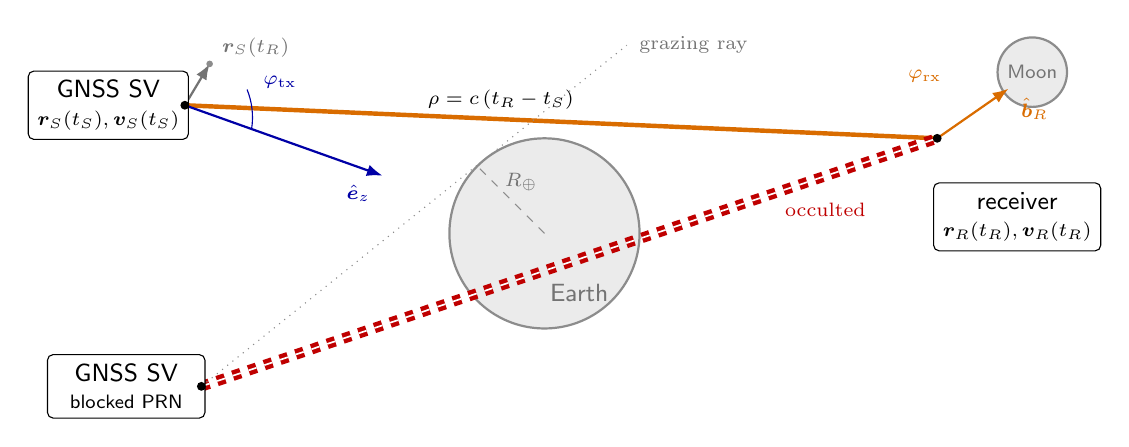
\begin{tikzpicture}[x=1.05cm, y=1.05cm, >=Latex]

    % --- occluding body (Earth) -------------------------------------------
    \fill[black!8] (0,0) circle (1.15);
    \draw[thick, black!45] (0,0) circle (1.15);
    \node[font=\small\sffamily, black!55] at (0.42,-0.72) {Earth};
    \draw[black!45, dashed] (0,0) -- (-0.81,0.81);
    \node[font=\scriptsize, black!55] at (-0.28,0.62) {$R_\oplus$};

    % --- receiver body (Moon) ---------------------------------------------
    \fill[black!8] (5.9,1.95) circle (0.42);
    \draw[thick, black!45] (5.9,1.95) circle (0.42);
    \node[font=\scriptsize\sffamily, black!55] at (5.9,1.95) {Moon};

    % --- transmitter at t_S and at t_R ------------------------------------
    \coordinate (TS) at (-4.35,1.55);
    \coordinate (TR) at (-4.05,2.05);
    \coordinate (RX) at (4.75,1.15);
    \coordinate (TB) at (-4.15,-1.85);

    % visible link
    \draw[model] (TS) -- (RX);
    \node[font=\scriptsize, above, sloped] at ($ (TS)!0.42!(RX) $)
      {$\rho = c\,(t_R - t_S)$};

    % transmitter motion during the light time
    \draw[flow, black!55] (TS) -- (TR);
    \node[font=\scriptsize, black!55, above right=-1pt and 1pt] at (TR)
      {$\vec{r}_S(t_R)$};

    % nadir / boresight of the transmitter
    \draw[flow, blue!65!black] (TS) -- ($ (TS)!0.55!(0,0) $);
    \node[font=\scriptsize, blue!65!black, below left=0pt and 1pt]
      at ($ (TS)!0.55!(0,0) $) {$\uvec{e}_z$};
    \draw[blue!65!black] ($ (TS)!0.9cm!(0,0) $) arc (-9:22:0.9);
    \node[font=\scriptsize, blue!65!black] at ($ (TS)+(1.15,0.28) $)
      {$\varphi_{\mathrm{tx}}$};

    % occulted link
    \draw[integral, red!75!black, dashed] (TB) -- (RX);
    \node[font=\scriptsize, red!75!black, below right, sloped]
      at ($ (TB)!0.78!(RX) $) {occulted};

    % grazing / tangent ray from the blocked transmitter
    \draw[black!45, dotted] (TB) -- ($ (TB)!1.5!(-0.72,0.90) $);
    \node[font=\scriptsize, black!55, right=1pt]
      at ($ (TB)!1.5!(-0.72,0.90) $) {grazing ray};

    % receiver boresight
    \draw[flow, orange!85!black] (RX) -- ($ (RX)!0.75!(5.9,1.95) $);
    \node[font=\scriptsize, orange!85!black, below right=0pt and 1pt]
      at ($ (RX)!0.75!(5.9,1.95) $) {$\uvec{b}_R$};
    \node[font=\scriptsize, orange!85!black] at ($ (RX)+(-0.15,0.75) $)
      {$\varphi_{\mathrm{rx}}$};

    % --- nodes -------------------------------------------------------------
    \node[boxnode, minimum width=2.0cm, anchor=east] at ($ (TS)+(0.05,0) $)
      {GNSS SV\\[-1pt]{\scriptsize $\vec{r}_S(t_S),\vec{v}_S(t_S)$}};
    \node[boxnode, minimum width=2.0cm, anchor=east] at ($ (TB)+(0.05,0) $)
      {GNSS SV\\[-1pt]{\scriptsize blocked PRN}};
    \node[boxnode, minimum width=1.9cm, anchor=west] at ($ (RX)+(-0.05,-0.95) $)
      {receiver\\[-1pt]{\scriptsize $\vec{r}_R(t_R),\vec{v}_R(t_R)$}};

    \fill (TS) circle (1.6pt);
    \fill[black!45] (TR) circle (1.2pt);
    \fill (TB) circle (1.6pt);
    \fill (RX) circle (1.6pt);

  \end{tikzpicture}
  \caption{Transmit/receive geometry. The signal leaves the transmitter at
    $t_S$ and arrives at $t_R$; during the light time the transmitter moves to
    $\vec{r}_S(t_R)$, and it is the \emph{retarded} state that enters the
    observation equations. The transmit antenna gain is evaluated at the
    off-boresight angle $\varphi_{\mathrm{tx}}$ from the nadir axis
    $\uvec{e}_z$ of the yaw-steering body frame, and the receive gain at
    $\varphi_{\mathrm{rx}}$ from the receiver boresight $\uvec{b}_R$. The
    lower PRN is rejected because the Earth blocks the line of sight.}
  \label{fig:gnss-geometry}
\end{figure}

\begin{lupntnote}
  All three of $\vec{r}_R$, $\vec{v}_R$ and $\vec{r}_S$, $\vec{v}_S$ are in
  the same inertial frame, so \cref{eq:gnss-rangerate} is the full inertial
  range rate. No Sagnac term appears, because none is needed: the Sagnac
  correction is exactly the difference between an Earth-fixed and an inertial
  formulation, and this model never leaves the inertial frame.
\end{lupntnote}

% ===========================================================================
\section{Clock Terms}
\label{sec:gnss-clocks}

\subsection{Receiver clock}

The receiver clock bias and drift enter as a range and a range-rate offset,
\begin{equation}
  \label{eq:gnss-rx-clock}
  \Delta\rho_R = c\,\Delta t_R, \qquad
  \Delta\dot\rho_R = c\,\dot{\Delta t}_R ,
\end{equation}
with $\Delta t_R > 0$ meaning the receiver clock \emph{leads} true time, which
makes the measured pseudorange longer than the geometric range. This is the
convention of \citet{misra2011gnss}: the receiver clock term is added.

\subsection{Transmitter clock}

The transmitter contributes three separate effects, combined into one
effective bias:
\begin{equation}
  \label{eq:gnss-tx-clock}
  \Delta t_S^{\mathrm{eff}}
  = \Delta t_S + \Delta t_S^{\mathrm{rel}} - \Delta t_S^{\mathrm{grp}} ,
  \qquad
  \dot{\Delta t}_S^{\mathrm{eff}} = \dot{\Delta t}_S ,
\end{equation}
and the corresponding range terms are
\begin{equation}
  \label{eq:gnss-tx-clock-range}
  \Delta\rho_S = c\,\Delta t_S^{\mathrm{eff}}, \qquad
  \Delta\dot\rho_S = c\,\dot{\Delta t}_S^{\mathrm{eff}} .
\end{equation}
The transmitter clock term is \emph{subtracted} from the observables: a
satellite clock that leads true time transmits early, so the signal arrives
having apparently travelled a shorter distance.

\begin{description}[leftmargin=1.4em,style=nextline,font=\normalfont\itshape]
  \item[$\Delta t_S$ --- \code{tx\_clock\_bias\_s}]
    The satellite clock offset. From SP3 it is the interpolated precise clock
    (which, in \cpp{Sp3Loader}, already contains the relativistic term); from
    BRDC it is the polynomial $a_{f0} + a_{f1}(t-t_{oc}) + a_{f2}(t-t_{oc})^2$
    of \citet{icdgps200}.
  \item[$\Delta t_S^{\mathrm{rel}}$ --- \code{relativistic\_correction\_s}]
    The periodic relativistic correction due to orbital eccentricity, in the
    state-based broadcast form
    \begin{equation}
      \label{eq:gnss-relativity}
      \Delta t_S^{\mathrm{rel}}
      = -\frac{2\,\vec{r}_S\transpose\vec{v}_S}{c^{2}} ,
    \end{equation}
    which is the Cartesian equivalent of the broadcast
    $-2\sqrt{\mu}\,e\sqrt{A}\sin E / c^2$. Its amplitude is
    $2 e \sqrt{\mu A}/c^2$, about \SI{23}{\nano\second} (\SI{7}{\meter}) for a
    GPS satellite with $e = 0.01$. Enabled by
    \code{options.apply\_transmitter\_relativity} (default true).
  \item[$\Delta t_S^{\mathrm{grp}}$ --- \code{group\_delay\_s}]
    The broadcast group delay $T_{GD}$ (or the constellation's BGD/TGD
    equivalent), which calibrates the satellite clock, defined on the
    ionosphere-free combination, to the single frequency actually tracked
    \citep{icdgps200}. It is subtracted from the effective bias, hence added
    to the pseudorange. \lupnt{} carries the field but does not populate it
    from the navigation message; it defaults to zero.
\end{description}

\begin{lstlisting}[language=cpp, caption={Effective transmitter clock terms.},
label={lst:gnss-tx-clock}]
// cpp/lupnt/measurements/gnss_measurement.cc :: GnssChannel
Real GnssChannel::EffectiveTransmitClockBiasSeconds() const {
  return tx_clock_bias_s + relativistic_correction_s - group_delay_s;
}
Real GnssChannel::EffectiveTransmitClockDrift() const { return tx_clock_drift; }

// cpp/lupnt/measurements/gnss_measurement.cc :: anonymous namespace
Real TransmitterRelativisticCorrectionSeconds(const Vec6& rv_tx) {
  return -2.0 * rv_tx.head(3).dot(rv_tx.tail(3)) / (Real(C) * Real(C));
}
\end{lstlisting}

\begin{lupntwarning}
  \cref{eq:gnss-relativity} must be evaluated in the frame in which the
  satellite clock is defined, i.e.\ Earth-centred inertial. The
  implementation applies it to \code{rv\_tx} \emph{after} conversion into
  \code{options.frame}. For \code{Frame::ECI} the two coincide; for a
  Moon-centred frame the product $\vec{r}_S\transpose\vec{v}_S$ is not the
  same quantity, and the correction is wrong by the difference. Runs that use
  a lunar measurement frame and also require the periodic relativistic term at
  the nanosecond level should supply the correction externally through
  \code{relativistic\_correction\_s} with
  \code{apply\_transmitter\_relativity = false}.
\end{lupntwarning}

% ===========================================================================
\section{Propagation Delays}
\label{sec:gnss-propagation}

\subsection{Shapiro delay}
\label{sec:gnss-shapiro}

When \code{options.apply\_shapiro\_delay} is true (the default), the one-way
gravitational (Shapiro) delay of the Sun is added as a range correction,
\begin{equation}
  \label{eq:gnss-shapiro}
  \Delta\rho_{\mathrm{Sh}}
  = \frac{2\mu_\odot}{c^{2}}
    \ln\!\left(
      \frac{r_R^{\odot} + r_S^{\odot} + \rho}
           {r_R^{\odot} + r_S^{\odot} - \rho}
    \right),
  \qquad
  \begin{aligned}
    r_R^{\odot} &= \lVert \vec{r}_R - \vec{r}_\odot(t_R) \rVert, \\
    r_S^{\odot} &= \lVert \vec{r}_S - \vec{r}_\odot(t_R) \rVert .
  \end{aligned}
\end{equation}
It is non-dispersive and always positive, so it is added to \emph{both} the
code and the carrier observable. The Sun position $\vec{r}_\odot(t_R)$ comes
from \cpp{SetSunPositionProvider}; with no provider installed the model falls
back to a fixed placeholder $(0, \SI{1}{\au}, 0)$, which is adequate for the
magnitude of the term but not for anything else. For a cislunar link
$2\mu_\odot/c^2 \approx \SI{2.95}{\kilo\meter}$ multiplies a logarithm of
order \num{1e-5}, giving a few centimetres.

\begin{lstlisting}[language=cpp, caption={Shapiro delay, guarded against the
degenerate geometry where the log argument is non-positive.},
label={lst:gnss-shapiro}]
// cpp/lupnt/measurements/gnss_measurement.cc :: GNSSMeasurements::ComputeShapiroDelay
Vec3 r_sun = SunPosition(receive_time);
Real rx_norm = (r_rx_eci - r_sun).norm();
Real tx_norm = (r_tx_eci - r_sun).norm();
Real rho = (r_rx_eci - r_tx_eci).norm();
if (rx_norm <= 0.0 || tx_norm <= 0.0) return Real(0.0);

Real numerator = rx_norm + tx_norm + rho;
Real denominator = rx_norm + tx_norm - rho;
if (denominator <= 0.0 || numerator <= 0.0) return Real(0.0);

return 2.0 * Real(GM_SUN) / (Real(C) * Real(C)) * log(numerator / denominator);
\end{lstlisting}

Only the Sun is modelled. The \code{shapiro\_mu} and
\code{shapiro\_body\_position} option fields are deprecated placeholders and
are not read. Earth's contribution to a cislunar link is a few millimetres and
is omitted.

\subsection{Ionospheric and plasmaspheric delay}
\label{sec:gnss-plasma}

The dispersive delay of the terrestrial ionosphere and plasmasphere is the
dominant medium error for a lunar receiver looking back through the Earth's
plasma envelope. It is represented as a positive \emph{code} delay in metres,
\begin{equation}
  \label{eq:gnss-plasma}
  \Delta\rho_{\mathrm{pl}}
  = \frac{40.3}{f^{2}} \int_\Gamma n_e \,\dd s \;\ge\; 0 ,
\end{equation}
with $n_e$ the electron density along the (possibly bent) ray path $\Gamma$,
$f$ in \si{\hertz} and $\Delta\rho_{\mathrm{pl}}$ in \si{\meter} when the
integral is in \si{\per\meter\squared}. Being dispersive, it advances the
carrier by as much as it delays the code:
\begin{equation}
  \label{eq:gnss-plasma-sign}
  \text{code observable uses } +\Delta\rho_{\mathrm{pl}},
  \qquad
  \text{carrier observable uses } -\Delta\rho_{\mathrm{pl}} .
\end{equation}
This is the code--carrier divergence that a dual-frequency or
carrier-smoothing algorithm exploits.

The term is \emph{disabled by default}
(\code{options.apply\_ionosphere\_plasma\_delay = false}). When enabled,
\cpp{ComputeIonospherePlasmaDelay} dispatches in strict priority order:

\begin{enumerate}[leftmargin=1.6em,itemsep=1pt]
  \item \cpp{SetCustomIonospherePlasmaDelayModel} --- a per-link callback
    $(t_R, \vec{r}_R, \vec{r}_S, f) \mapsto \Delta\rho_{\mathrm{pl}}$;
  \item \cpp{SetIonospherePlasmaRayTraceOptions} --- the built-in
    GCPM/IRI ray tracer in
    \file{cpp/lupnt/environment/plasma/tec/raytrace.cc}, returning either the
    TEC-only delay or TEC plus the second- and third-order terms according to
    \code{delay\_mode};
  \item \code{options.default\_ionosphere\_plasma\_delay\_m} --- a constant.
\end{enumerate}

The batch variant \cpp{SetBatchCustomIonospherePlasmaDelayModel} is evaluated
once for all epochs and channels; see \cref{sec:gnss-precompute}. The
electron-density model, the ray-bending integration and the higher-order terms
are specified in full in \cref{chap:ionosphere}; this chapter fixes only
\cref{eq:gnss-plasma-sign}, the interface, and the unit (metres of code delay
at the channel frequency).

\begin{lupntnote}
  The ray tracer works in geocentric Earth-fixed coordinates
  (\code{raytrace\_frame = Frame::ECEF}) and expects $\UTC$ seconds from J2000
  (\code{raytrace\_epoch\_scale = Time::UTC}), so the measurement model
  converts both endpoints and the epoch before calling it, and converts
  nothing back --- the delay is a scalar. Positions are passed in
  \si{\kilo\meter}.
\end{lupntnote}

\subsection{Tropospheric delay}
\label{sec:gnss-tropo}

The troposphere is non-dispersive and is added to both observables with the
same sign as the Shapiro term. \lupnt{} implements the Saastamoinen zenith
delay with a $1/\sin e$ mapping \citep{saastamoinen1972},
\begin{equation}
  \label{eq:gnss-tropo}
  \Delta\rho_{\mathrm{tr}}
  = \frac{1}{\sin e}
    \left[
      \frac{\num{0.0022768}\,P}{f(\varphi, h)}
      + \frac{\num{0.0022768}}{f(\varphi, h)}
        \left( \frac{1255}{T} + 0.05 \right) e_w
    \right],
\end{equation}
with $e$ the elevation angle, $P$ the total pressure in \si{\hecto\pascal},
$T$ the temperature in \si{\kelvin}, $e_w$ the water-vapour partial pressure
from a Tetens saturation formula, and
$f(\varphi,h) = 1 - \num{0.00266}\cos 2\varphi - \num{2.8e-7} h$ the
latitude/height gravity factor. The horizon singularity is guarded by clamping
$\sin e \ge \num{1e-3}$.

\begin{lupntwarning}
  \cref{eq:gnss-tropo} lives in
  \file{cpp/lupnt/measurements/ground_station_corrections.cc}
  (\cpp{TroposphereDelaySaastamoinen}) and is used by the ground-station
  tracking application, \emph{not} by \cpp{GNSSMeasurements}. The GNSS channel
  has no troposphere field: the model targets space receivers, whose links do
  not traverse the neutral atmosphere. A ground-based GNSS receiver simulated
  with this model will be missing \SIrange{2.3}{25}{\meter} of delay
  depending on elevation.
\end{lupntwarning}

\subsection{Phase wind-up}
\label{sec:gnss-windup}

A right-hand circularly polarised carrier accumulates one cycle of phase per
relative rotation of the transmit and receive antennas about the line of
sight. The standard model is
\begin{equation}
  \label{eq:gnss-windup}
  \Delta\phi_{\mathrm{wu}}
  = \operatorname{sign}\!\bigl(\uvec{u}\transpose(\uvec{D}_S\times\uvec{D}_R)\bigr)
    \cos^{-1}\!\left(
      \frac{\uvec{D}_S\transpose\uvec{D}_R}
           {\lVert \uvec{D}_S\rVert\,\lVert \uvec{D}_R\rVert}
    \right)
  \quad\text{[cycle]},
\end{equation}
with $\uvec{D}_S$ and $\uvec{D}_R$ the effective dipole vectors of the two
antennas projected onto the plane normal to $\uvec{u}$, unwrapped in time
against the previous epoch. \lupnt{} does \emph{not} implement
\cref{eq:gnss-windup}: there is no wind-up term anywhere in the measurement
code. Its effect is absorbed into \code{phase\_bias\_cycles} and, over an arc,
into the estimated ambiguity, which is acceptable while the receiver attitude
is slowly varying and no cycle-slip reset occurs. It is listed here because it
is the largest \emph{unmodelled} carrier-phase term for a spinning or
rapidly slewing receiver --- up to one full cycle, i.e.\ \SI{19}{\centi\meter}
at L1, per revolution.

% ===========================================================================
\section{Observation Equations}
\label{sec:gnss-observables}

Collecting the pieces, with $\lambda = c/f$ and the clock range terms of
\cref{eq:gnss-rx-clock,eq:gnss-tx-clock-range}, the three observables are as
follows. Each is emitted only if its \code{GnssObservable} appears in
\code{options.observables}; the default is all three, in the order
pseudorange, Doppler, carrier phase.

\subsection{Pseudorange}

\begin{equation}
  \label{eq:gnss-pseudorange}
  \boxed{\;
  P = \rho
    + \Delta\rho_{\mathrm{Sh}}
    + \Delta\rho_{\mathrm{pl}}
    + \Delta\rho_R
    - \Delta\rho_S \;}
  \qquad [\si{\meter}]
\end{equation}

Every term is in metres. The geometric range $\rho$ is the light-time-corrected
range \cref{eq:gnss-range}; the Shapiro and plasma delays are added because
both retard the code; the receiver clock is added and the effective
transmitter clock (bias plus relativity minus group delay) subtracted per
\cref{sec:gnss-clocks}.

\subsection{Doppler}

\begin{equation}
  \label{eq:gnss-doppler}
  \boxed{\;
  D = -\frac{\dot\rho + \Delta\dot\rho_R - \Delta\dot\rho_S}{\lambda} \;}
  \qquad [\si{\hertz}]
\end{equation}

The leading minus sign follows from the $\uvec{u}$ convention of
\cref{sec:gnss-geometry}: an opening link ($\dot\rho > 0$) produces a negative
frequency shift. $D$ is the shift of the received carrier relative to the
nominal frequency $f$, not the received frequency itself. Multiplying by
$-\lambda$ recovers the pseudorange rate in \si{\meter\per\second}, which is
the form the Endurance-style single-satellite Doppler navigation problem uses.

\subsection{Carrier phase}

\begin{equation}
  \label{eq:gnss-carrier}
  \boxed{\;
  \Phi = \frac{\rho
    + \Delta\rho_{\mathrm{Sh}}
    - \Delta\rho_{\mathrm{pl}}
    + \Delta\rho_R
    - \Delta\rho_S}{\lambda}
    + \phi_0 \;}
  \qquad [\text{cycle}]
\end{equation}

with $\phi_0 = \code{phase\_bias\_cycles}$ the fractional (non-integer) bias
lumping the transmit and receive hardware phase offsets and, in this model,
the unmodelled wind-up. Note the sign flip on $\Delta\rho_{\mathrm{pl}}$
relative to \cref{eq:gnss-pseudorange}. When an integer ambiguity is present
--- either in the channel (\code{integer\_ambiguity\_cycles}) or, taking
precedence, in the state at \code{indices.carrier\_integer} --- the emitted
observable is
\begin{equation}
  \label{eq:gnss-carrier-meas}
  \Phi_{\mathrm{meas}} = \Phi + N .
\end{equation}

\cref{tab:gnss-signs} summarises the sign convention for every term, which is
the single most error-prone part of any GNSS implementation.

\begin{table}[htbp]
  \centering
  \caption{Sign of each term in the three observables. ``$+$'' means the term
    increases the observable as written; entries in the Doppler column refer
    to the bracketed range-rate sum of \cref{eq:gnss-doppler}, before the
    overall $-1/\lambda$.}
  \label{tab:gnss-signs}
  \begin{tabular}{llccc}
    \toprule
    Term & Field & $P$ & $[\,\cdot\,]$ of $D$ & $\Phi$ \\
    \midrule
    geometric range / rate   & ---                             & $+\rho$ & $+\dot\rho$ & $+\rho/\lambda$ \\
    receiver clock           & state \code{clock\_bias/drift}  & $+$ & $+$ & $+$ \\
    transmitter clock        & \code{tx\_clock\_bias\_s}       & $-$ & $-$ & $-$ \\
    transmitter relativity   & \code{relativistic\_correction\_s} & $-$ & $\cdot$ & $-$ \\
    group delay              & \code{group\_delay\_s}          & $+$ & $\cdot$ & $+$ \\
    Shapiro                  & \code{shapiro\_delay\_m}        & $+$ & $\cdot$ & $+$ \\
    ionosphere / plasma      & \code{ionosphere\_plasma\_delay\_m} & $+$ & $\cdot$ & $-$ \\
    fractional phase bias    & \code{phase\_bias\_cycles}      & $\cdot$ & $\cdot$ & $+$ \\
    integer ambiguity        & \code{integer\_ambiguity\_cycles} & $\cdot$ & $\cdot$ & $+$ \\
    \bottomrule
  \end{tabular}
\end{table}

The whole of \cref{eq:gnss-pseudorange,eq:gnss-doppler,eq:gnss-carrier} is
sixteen lines of code:

\begin{lstlisting}[language=cpp, caption={The three observables.},
label={lst:gnss-observables}]
// cpp/lupnt/measurements/gnss_measurement.cc :: GnssMeasurement::ComputeValue
Vec3 dr = r_rx - r_tx;
Vec3 dv = v_rx - v_tx;
Real rho = dr.norm();
Real rho_dot = dr.dot(dv) / rho;

Real tx_bias_m  = C * channel_.EffectiveTransmitClockBiasSeconds();
Real tx_drift_mps = C * channel_.EffectiveTransmitClockDrift();
Real code_delay_m    = channel_.shapiro_delay_m + channel_.ionosphere_plasma_delay_m;
Real carrier_delay_m = channel_.shapiro_delay_m - channel_.ionosphere_plasma_delay_m;
Real range_with_clock      = rho + code_delay_m + rx_bias_m - tx_bias_m;
Real range_rate_with_clock = rho_dot + rx_drift_mps - tx_drift_mps;
Real lambda = channel_.Wavelength();

value.pseudorange_m = range_with_clock;
value.doppler_hz = -range_rate_with_clock / lambda;
value.carrier_phase_cycles
    = (rho + carrier_delay_m + rx_bias_m - tx_bias_m) / lambda + channel_.phase_bias_cycles;
value.carrier_integer_cycles = integer_cycles;
\end{lstlisting}

\begin{lupntnote}
  The Doppler observable contains no time derivative of the Shapiro or plasma
  delay. $\dd\Delta\rho_{\mathrm{Sh}}/\dd t$ is of order
  \SI{1e-5}{\meter\per\second} and negligible;
  $\dd\Delta\rho_{\mathrm{pl}}/\dd t$ can reach
  \SIrange{0.01}{0.1}{\meter\per\second} at low geocentric altitude and is a
  genuine omission for Doppler-only navigation through the plasmasphere.
\end{lupntnote}

\subsection{Time-differenced carrier phase}
\label{sec:gnss-tdcp}

The Lunar GNSS ODTS scenario also forms a time-differenced carrier phase
(TDCP) observable, expressed as a carrier \emph{range} difference in metres
between consecutive epochs,
\begin{equation}
  \label{eq:gnss-tdcp}
  \Delta\Phi_{k,k-1}
  = \lambda\bigl(\Phi_k - \Phi_{k-1}\bigr)
  = \bigl(\rho_k - \rho_{k-1}\bigr)
  + \bigl(\Delta\rho_{R,k} - \Delta\rho_{R,k-1}\bigr)
  - \bigl(\Delta\rho_{S,k} - \Delta\rho_{S,k-1}\bigr)
  + \cdots ,
\end{equation}
in which the ambiguity $N$ and the fractional bias $\phi_0$ cancel exactly as
long as lock is maintained. Because \cref{eq:gnss-tdcp} depends on both the
current and the previous receiver state, it cannot be processed by a plain
Kalman update; \lupnt{} processes it with the UDU stochastic-cloning filter
\citep{iiyama2026scud}, which carries a clone of the previous state in the
augmented vector. The lunar TDCP positioning and timekeeping results this
supports are those of \citet{iiyama2024navi}.

% ===========================================================================
\section{Visibility, Occultation and Channel Gating}
\label{sec:gnss-visibility}

Given a receiver state, \cpp{BuildChannels} walks every PRN of every attached
constellation and applies four gates in order. A PRN that fails any gate
contributes no rows to the measurement vector at that epoch, so the
measurement dimension changes from epoch to epoch.

\begin{figure}[htbp]
  \centering
  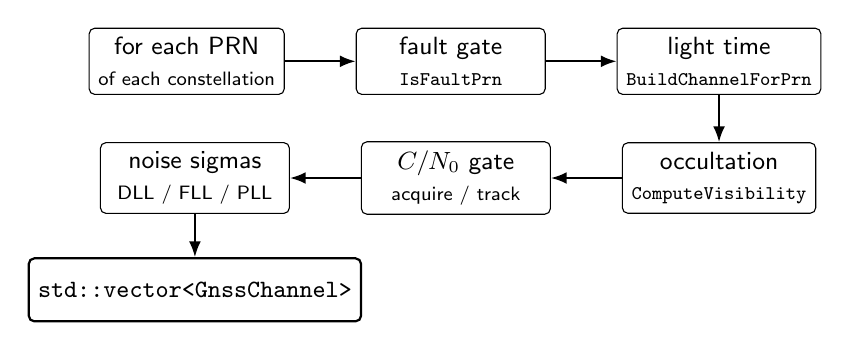
\begin{tikzpicture}[node distance=6mm and 9mm, >=Latex]
    \node[boxnode] (prn)  {for each PRN\\{\scriptsize of each constellation}};
    \node[boxnode, right=of prn] (fault) {fault gate\\{\scriptsize \code{IsFaultPrn}}};
    \node[boxnode, right=of fault] (build) {light time\\{\scriptsize \cpp{BuildChannelForPrn}}};
    \node[boxnode, below=of build] (vis) {occultation\\{\scriptsize \cpp{ComputeVisibility}}};
    \node[boxnode, left=of vis] (cn0) {$C/N_0$ gate\\{\scriptsize acquire / track}};
    \node[boxnode, left=of cn0] (sig) {noise sigmas\\{\scriptsize DLL / FLL / PLL}};

    \draw[flow] (prn) -- (fault);
    \draw[flow] (fault) -- (build);
    \draw[flow] (build) -- (vis);
    \draw[flow] (vis) -- (cn0);
    \draw[flow] (cn0) -- (sig);
    \draw[flow] (sig.south) -- ++(0,-0.55)
      node[boxnode, below, minimum width=3.1cm, anchor=north]
      {\code{std::vector<GnssChannel>}};
  \end{tikzpicture}
  \caption{Channel construction and gating inside
    \cpp{GNSSMeasurements::BuildChannels}. Each gate can drop the PRN; the
    surviving channels define the rows of the measurement vector at that
    epoch.}
  \label{fig:gnss-pipeline}
\end{figure}

\subsection{Fault gate}

PRNs registered with \cpp{SetFaultPrns} are skipped before any geometry is
computed. This is how a satellite outage or a clock-fault scenario is injected
for the fault-monitoring studies.

\subsection{Body-blocking test}
\label{sec:gnss-occultation}

Each entry of \cpp{SetOccludingBodies} is a sphere: a radius, and either a
fixed centre or a per-epoch position callback evaluated once per epoch (not
once per PRN). \cpp{ComputeVisibility}
(\file{cpp/lupnt/measurements/comms_utils.cc}) then runs two regimes.

\paragraph{Near-surface endpoints.} An endpoint with
$\lVert \vec{r} - \vec{r}_{\mathrm{body}} \rVert < R + h_{\min}$ (default
$h_{\min} = \SI{10}{\kilo\meter}$) is treated as a surface point, and the test
becomes an elevation mask. With $\vec{r}_{12} = \vec{r}_2 - \vec{r}_1$ and
$\vec{r}_{1b} = \vec{r}_{\mathrm{body}} - \vec{r}_1$,
\begin{equation}
  \label{eq:gnss-elevation}
  e = \cos^{-1}\!\left(
      \frac{\vec{r}_{12}\transpose \vec{r}_{1b}}
           {\lVert\vec{r}_{12}\rVert\,\lVert\vec{r}_{1b}\rVert}
    \right) - \frac{\pi}{2},
  \qquad
  \text{visible} \iff e > e_{\min} .
\end{equation}
$e$ is measured from the local horizon plane, positive upward. The default
mask is $e_{\min} = \SI{5}{\degree}$; the lunar-surface studies of
\citet[Ch.~6]{iiyama2026thesis} relax it to $\SI{-10}{\degree}$ to admit the
grazing rays that dominate a lunar user's sidelobe geometry.

\paragraph{Space-to-space links.} If neither endpoint is near the surface, the
test is a tangent-line occlusion test. With $\vec{r} = \vec{r}_2 - \vec{r}_1$
and $\vec{r}_{1b} = \vec{r}_1 - \vec{r}_{\mathrm{body}}$,
\begin{align}
  \label{eq:gnss-tangent}
  \theta_1 &= \cos^{-1}\!\left(
      \frac{-\vec{r}_{1b}\transpose\vec{r}}
           {\lVert\vec{r}\rVert\,\lVert\vec{r}_{1b}\rVert} \right),
  &
  \theta_2 &= \sin^{-1}\!\left(
      \frac{R}{\lVert\vec{r}_{1b}\rVert} \right),
  &
  d_{\mathrm{hor}} &= \sqrt{\lVert\vec{r}_{1b}\rVert^2 - R^2},
\end{align}
and the link is \emph{blocked} when
\begin{equation}
  \label{eq:gnss-occulted}
  \theta_1 < \theta_2
  \quad\text{and}\quad
  \lVert\vec{r}\rVert > d_{\mathrm{hor}} .
\end{equation}
$\theta_2$ is the angular radius of the body seen from $\vec{r}_1$ and
$\theta_1$ the angle between the line of sight and the direction to the body
centre, so the first condition says the ray points inside the body's angular
disc; the second says the far endpoint is beyond the tangent point rather than
in front of the body. Both are needed --- a receiver between the transmitter
and the body is not occulted even though the ray points at the body.

\begin{lstlisting}[language=cpp, caption={Space-to-space occultation test.},
label={lst:gnss-visibility}]
// cpp/lupnt/measurements/comms_utils.cc :: ComputeVisibility
Vec3 r = r2 - r1;
Real r_norm = r.norm();
Vec3 r1body = r1 - r_body;
Real dot_r_r1b = -r1body.dot(r);
Real theta1 = acos(clamp(dot_r_r1b / r_norm / r1body_norm, -1.0, 1.0));
Real theta2 = asin(clamp(R_body / r1body_norm, -1.0, 1.0));
Real r1_to_horizon = sqrt(r1body_norm * r1body_norm - R_body * R_body);
if (theta1 < theta2 && r_norm > r1_to_horizon) return false;

return true;
\end{lstlisting}

The body is a sphere with no atmosphere and no terrain: the test is purely
geometric, and an Earth-limb-grazing ray is declared visible with no
refraction, defocusing or atmospheric attenuation applied. For lunar users the
Moon is entered with its mean radius $R = \code{R\_MOON}$, so terrain relief of
a few kilometres is absorbed into the sphere radius.

\subsection{Boresight angles and the transmitter body frame}
\label{sec:gnss-attitude}

A surviving link still has to be strong enough to track, and the transmit gain
of a GNSS satellite varies by \SI{30}{\dB} between the main lobe and the
sidelobes a lunar receiver actually uses. The gain is a table lookup in the
satellite's yaw-steering body frame, so that frame must be built first.

\cpp{ComputeCN0} transforms the transmitter state, the receiver position and
the Sun position from \code{options.frame} into \code{Frame::GCRF} before
building the attitude, because ANTEX-derived patterns are defined in an
Earth-centred inertial frame. The orthonormal triad is
\begin{equation}
  \label{eq:gnss-attitude}
  \uvec{e}_z = \widehat{-\vec{r}_S}, \qquad
  \uvec{e}_y = \widehat{\uvec{e}_z \times \widehat{(\vec{r}_\odot - \vec{r}_S)}}, \qquad
  \uvec{e}_x = \widehat{\uvec{e}_y \times \uvec{e}_z},
\end{equation}
i.e.\ $\uvec{e}_z$ along nadir (the antenna boresight), $\uvec{e}_y$ along the
solar-panel axis and $\uvec{e}_x$ completing the right-handed triad. The
off-boresight and azimuth angles of the transmitter-to-receiver line of sight
$\uvec{u}$ are then
\begin{equation}
  \label{eq:gnss-boresight}
  \varphi_{\mathrm{tx}} = \cos^{-1}\!\bigl(\uvec{u}\transpose\uvec{e}_z\bigr),
  \qquad
  \theta_{\mathrm{tx}} = \atantwo\!\bigl(\uvec{u}\transpose\uvec{e}_y,\ \uvec{u}\transpose\uvec{e}_x\bigr),
\end{equation}
and the receiver off-boresight angle, measured from the receiver's pointing
target $\vec{b}$ (the Moon or Earth centre, supplied by
\cpp{SetBoresightTargetProvider}), is
\begin{equation}
  \label{eq:gnss-boresight-rx}
  \varphi_{\mathrm{rx}}
  = \cos^{-1}\!\left(
      \widehat{(\vec{b} - \vec{r}_R)}\transpose\,\widehat{(\vec{r}_S - \vec{r}_R)}
    \right).
\end{equation}

The velocity-aware overload derives the same frame from the documented nominal
yaw-steering law,
\begin{equation}
  \label{eq:gnss-yaw}
  \psi_{\mathrm{nom}} = \atantwo\bigl(-\tan\beta,\ \sin\mu\bigr),
\end{equation}
with $\beta$ the Sun elevation above the orbital plane and $\mu$ the orbit
angle from the midnight point, then rotates the orbital reference frame
($\uvec{e}_x^{\mathrm{ref}} = \widehat{\vec{v}_S}$) about nadir by
$\psi_{\mathrm{nom}}$. The two constructions are numerically identical, since
the nominal yaw law is by definition the yaw that keeps the panels
Sun-pointing \citep{kouba2009yaw,cheng2025yaw}.

\begin{lstlisting}[language=cpp, caption={Body frame, boresight angles and
link budget for one channel.}, label={lst:gnss-cn0}]
// cpp/lupnt/measurements/gnss_measurement.cc :: GNSSMeasurements::ComputeCN0
GnssAttitude::Compute(rv_tx_gcrf.head(3), Vec3(rv_tx_gcrf.tail(3)), r_sun_gcrf, ex, ey, ez);
Real phi_tx = safe_acos(u_tx2rx_gcrf.dot(ez));
Real theta_tx = atan2(u_tx2rx_gcrf.dot(ey), u_tx2rx_gcrf.dot(ex));
Real phi_rx = safe_acos(u_rx2body.dot(u_rx2tx));

Real G_tx = constellation->GetTransmitterAntenna(channel.prn, channel.frequency)
                .ComputeGain(theta_tx, phi_tx);
Real G_rx = rx_antenna_.ComputeGain(0.0, phi_rx);
Real P_tx = constellation->GetTransmitPowerDbw(channel.prn, channel.frequency);

return LinkBudget(P_tx, G_tx, G_rx, range, channel.frequency, rx_params_);
\end{lstlisting}

Setting \code{options.tx\_yaw\_model = TxYawModel::DEDICATED} replaces
\cref{eq:gnss-yaw} with the block-specific eclipse yaw law of
\cpp{GnssYawSteering}
(\cpp{Gps3EclipseYawAngle} for GPS,
\cpp{GalileoIovEclipseYawAngle} for Galileo, nominal otherwise), evaluated
continuously from geometry. These laws differ from nominal only near the
orbit noon/midnight singularity at small $\beta$, where the real satellite
rate-limits its yaw; because there is no maneuver-window state machine, the
result approximates the eclipse-season attitude rather than reproducing a
maneuver schedule. \citet[Ch.~6.4.3]{iiyama2026thesis} assumes nominal yaw
steering throughout.

\subsection{Antenna gain gating}
\label{sec:gnss-gain}

\cpp{Antenna::ComputeGain} (\file{cpp/lupnt/measurements/antenna.cc})
interpolates the measured pattern, wrapping $\theta$ to $[0,360]^\circ$ and
$\varphi$ to $[-180,180]^\circ$:

\begin{lstlisting}[language=cpp, caption={Pattern lookup, with the implicit
sidelobe cutoff.}, label={lst:gnss-antenna}]
// cpp/lupnt/measurements/antenna.cc :: Antenna::ComputeGain
Real gain = 0.0;
if (n_dim_ == 0) return gain;                       // omni antenna: G == 0 dB
theta = WrapToTwoPi(theta) * DEG;
phi = WrapToPi(phi) * DEG;
if (phi > phi_max_ || phi < -phi_max_) return NAN;  // off-pattern -> NaN
if (phi < 0 && phi_(0) >= 0) phi = -phi;            // symmetry
if (n_dim_ == 2) gain = LinearInterp2d(phi_, theta_, gain_, phi.val(), theta.val());
else if (n_dim_ == 1) gain = LinearInterp1d(phi_, gain_, phi.val());
return gain;
\end{lstlisting}

An empty antenna name gives an omnidirectional pattern ($G \equiv 0$
\si{\dB}), and a direction outside the tabulated $\varphi$ range returns
\code{NaN}. The \code{NaN} propagates through the link budget, and the
gate below drops the channel, so the pattern's angular extent acts as an
implicit sidelobe cutoff. The same happens when
\cpp{HasTransmitterInfo} is false for a PRN/frequency pair: $C/N_0$ is
\code{NaN} and the channel is dropped.

The received carrier-to-noise density follows the closed-form budget
\citep[Eq.~6.59]{iiyama2026thesis}
\begin{equation}
  \label{eq:gnss-cn0}
  \left(\frac{C}{N_0}\right)_{\si{\dBHz}}
  = P_{\mathrm{tx}}
  + G_{\mathrm{tx}}(\theta_{\mathrm{tx}}, \varphi_{\mathrm{tx}})
  + G_{\mathrm{rx}}(\varphi_{\mathrm{rx}})
  - L_{\mathrm{fs}} - L_{\mathrm{atm}} - L_{\mathrm{ad}} - L_{\mathrm{pol}}
  - 10\log_{10} k_B - 10\log_{10} T_{\mathrm{eff}} ,
\end{equation}
with $L_{\mathrm{fs}} = 20\log_{10}(4\pi \rho f / c)$ the free-space path
loss. The EIRP values, the measured gain patterns and the mapping from
$C/N_0$ to the DLL, FLL and PLL noise standard deviations are specified in
\cref{chap:link-budget}; here they matter only through the gate and through
the diagonal of the measurement covariance.

\subsection{Acquisition and tracking hysteresis}

The $C/N_0$ gate is stateful. A PRN not currently in lock must exceed the
acquisition threshold; one already in lock need only exceed the (lower)
tracking threshold:
\begin{equation}
  \label{eq:gnss-cn0-gate}
  \text{keep} \iff
  \frac{C}{N_0} >
  \begin{cases}
    (C/N_0)_{\mathrm{acq}} = \SI{22}{\dBHz}, & \text{PRN not in lock},\\[2pt]
    (C/N_0)_{\mathrm{trk}} = \SI{20}{\dBHz}, & \text{PRN in lock}.
  \end{cases}
\end{equation}
The lock set \code{tracking\_prns\_} is rebuilt after every
\cpp{BuildChannels} call from the surviving channels, and is cleared by
\cpp{ResetTracking}. The \SI{2}{\dB} hysteresis reproduces the observed
behaviour of a real receiver that holds a weak satellite it has already
acquired, and prevents the rapid acquire/drop chatter that a single threshold
produces at the sidelobe boundaries. The comparison is written
\code{!(cn0 > threshold)}, so a \code{NaN} $C/N_0$ is dropped rather than
kept. Setting \code{options.apply\_cn0\_threshold = false} disables the gate
entirely, and \cpp{SetCN0Threshold} collapses both thresholds to one value
(the deprecated single-threshold behaviour).

% ===========================================================================
\section{Measurement Jacobians}
\label{sec:gnss-jacobian}

\cpp{GnssMeasurement::ComputeVector} returns $\vec{y} = h(\vec{x})$ and, when
asked, the analytic Jacobian $\mat{H} = \partial h/\partial\vec{x}$ with
$|\code{observables}|$ rows and $\dim\vec{x}$ columns, zero-initialised so
that any state component not named in \code{indices} keeps a zero column.

\subsection{Building blocks}

Differentiating \cref{eq:gnss-range,eq:gnss-rangerate} with respect to the
receiver position and velocity, holding the transmitter state fixed,
\begin{align}
  \label{eq:gnss-drho}
  \frac{\partial \rho}{\partial \vec{r}_R} &= \uvec{u}\transpose,
  &
  \frac{\partial \rho}{\partial \vec{v}_R} &= \vec{0}\transpose, \\
  \label{eq:gnss-drhodot}
  \frac{\partial \dot\rho}{\partial \vec{r}_R}
    &= \left( \frac{\Delta\vec{v}}{\rho}
       - \frac{\dot\rho\,\Delta\vec{r}}{\rho^{2}} \right)^{\!\mathsf{T}},
  &
  \frac{\partial \dot\rho}{\partial \vec{v}_R} &= \uvec{u}\transpose .
\end{align}
\cref{eq:gnss-drhodot} can equivalently be written
\begin{equation}
  \label{eq:gnss-drhodot-proj}
  \frac{\partial \dot\rho}{\partial \vec{r}_R}
  = \frac{1}{\rho}
    \left[ \bigl( \mat{I} - \uvec{u}\,\uvec{u}\transpose \bigr) \Delta\vec{v}
    \right]^{\mathsf{T}},
\end{equation}
which makes the structure explicit: only the component of the relative
velocity \emph{perpendicular} to the line of sight changes the range rate when
the receiver moves, and the sensitivity falls off as $1/\rho$.

The clock scale factors are the derivatives of \cref{eq:gnss-clock-units},
\begin{equation}
  \label{eq:gnss-clock-deriv}
  \frac{\partial \Delta\rho_R}{\partial b_R}
    = c\,\frac{\partial \Delta t_R}{\partial b_R}
    = \frac{c}{s(\text{unit})},
  \qquad
  \frac{\partial \Delta\dot\rho_R}{\partial d_R}
    = \frac{c}{s(\text{unit})},
\end{equation}
where $s(\text{unit})$ is the seconds-to-unit scale: $s = 1$ for
\code{SECONDS}, so the factor is $c$; $s = 1/c$ for \code{METERS}, so the
factor is $1$; and $s = \num{e-3}/c$ for \code{KILOMETERS}.

\subsection{Rows}

\begin{equation}
  \label{eq:gnss-jac-pseudorange}
  \frac{\partial P}{\partial \vec{r}_R} = \uvec{u}\transpose,
  \qquad
  \frac{\partial P}{\partial b_R} = \frac{c}{s},
  \qquad
  \frac{\partial P}{\partial \vec{v}_R} = \vec{0}\transpose,
  \qquad
  \frac{\partial P}{\partial d_R} = 0 ;
\end{equation}
\begin{equation}
  \label{eq:gnss-jac-doppler}
  \frac{\partial D}{\partial \vec{r}_R}
    = -\frac{1}{\lambda}\left( \frac{\Delta\vec{v}}{\rho}
       - \frac{\dot\rho\,\Delta\vec{r}}{\rho^{2}} \right)^{\!\mathsf{T}},
  \qquad
  \frac{\partial D}{\partial \vec{v}_R} = -\frac{1}{\lambda}\uvec{u}\transpose,
  \qquad
  \frac{\partial D}{\partial d_R} = -\frac{c}{\lambda s} ;
\end{equation}
\begin{equation}
  \label{eq:gnss-jac-carrier}
  \frac{\partial \Phi}{\partial \vec{r}_R} = \frac{1}{\lambda}\uvec{u}\transpose,
  \qquad
  \frac{\partial \Phi}{\partial b_R} = \frac{c}{\lambda s},
  \qquad
  \frac{\partial \Phi_{\mathrm{meas}}}{\partial N} = 1 .
\end{equation}

For the default eight-state layout $\vec{x} = [\vec{r}_R;\ \vec{v}_R;\ b_R;\
d_R]$ with the clock in seconds, the full single-channel Jacobian is
\begin{equation}
  \label{eq:gnss-jac-block}
  \mat{H} =
  \begin{bmatrix}
    \uvec{u}\transpose & \vec{0}\transpose & c & 0 \\[4pt]
    -\frac{1}{\lambda}\left(\frac{\Delta\vec{v}}{\rho}
      - \frac{\dot\rho\,\Delta\vec{r}}{\rho^{2}}\right)^{\!\mathsf{T}}
      & -\frac{1}{\lambda}\uvec{u}\transpose & 0 & -\frac{c}{\lambda} \\[6pt]
    \frac{1}{\lambda}\uvec{u}\transpose & \vec{0}\transpose & \frac{c}{\lambda} & 0
  \end{bmatrix},
\end{equation}
and \cpp{GNSSMeasurements::ComputeFromChannels} stacks one such block per
surviving channel, giving a $3 n_{\mathrm{ch}} \times \dim\vec{x}$ matrix at
that epoch.

\begin{lstlisting}[language=cpp, caption={Analytic Jacobian rows.},
label={lst:gnss-jacobian}]
// cpp/lupnt/measurements/gnss_measurement.cc :: GnssMeasurement::ComputeVector
Vec3 u = dr / rho;
Vec3 d_rhodot_dr = dv / rho - rho_dot * dr / (rho * rho);
Vec3 d_rhodot_dv = u;
Real db_m  = ClockBiasMetersDerivative(options.clock_bias_unit);
Real dd_mps = ClockDriftMetersPerSecondDerivative(options.clock_bias_unit);

case GnssObservable::PSEUDORANGE:
  H->block(row, idx.position, 1, 3) = ToRowVec3d(u);
  if (idx.clock_bias >= 0 && idx.clock_bias < user_state.size())
    (*H)(row, idx.clock_bias) = db_m.val();
  break;

case GnssObservable::DOPPLER:
  H->block(row, idx.position, 1, 3) = ToRowVec3d(-d_rhodot_dr / lambda);
  H->block(row, idx.velocity, 1, 3) = ToRowVec3d(-d_rhodot_dv / lambda);
  if (idx.clock_drift >= 0 && idx.clock_drift < user_state.size())
    (*H)(row, idx.clock_drift) = (-dd_mps / lambda).val();
  break;

case GnssObservable::CARRIER_PHASE:
  H->block(row, idx.position, 1, 3) = ToRowVec3d(u / lambda);
  if (idx.clock_bias >= 0 && idx.clock_bias < user_state.size())
    (*H)(row, idx.clock_bias) = (db_m / lambda).val();
  if (idx.carrier_integer >= 0 && idx.carrier_integer < user_state.size())
    (*H)(row, idx.carrier_integer) = 1.0;
  break;
\end{lstlisting}

\subsection{What the Jacobian omits}

\cref{eq:gnss-jac-block} is a \emph{partial} derivative that holds the
transmitter state, the delays and the noise model fixed. Omitted are:

\begin{itemize}[leftmargin=1.4em,itemsep=1pt]
  \item the light-time coupling
    $\partial \vec{r}_S / \partial \vec{r}_R
     = \vec{v}_S\,\uvec{u}\transpose / c$, of relative size
    $\lVert\vec{v}_S\rVert/c \approx \num{1.3e-5}$;
  \item $\partial \Delta\rho_{\mathrm{Sh}} / \partial \vec{r}_R$, of order
    \num{1e-9};
  \item $\partial \Delta\rho_{\mathrm{pl}} / \partial \vec{r}_R$, which is not
    even available in closed form for the ray-traced model;
  \item the dependence of $C/N_0$, and hence of the measurement covariance
    $\mat{R}$, on the receiver state --- a genuine effect near a gain-pattern
    null, but one that a Kalman filter is not structured to use anyway;
  \item any derivative with respect to the transmitter clock, since the
    transmitter clock is not estimated.
\end{itemize}

All of these are far below the linearisation error of an extended Kalman
filter at the position uncertainties of interest. When exact derivatives are
required, the whole model is written in the forward-mode \code{Real} scalar
type and can be differentiated end to end by automatic differentiation
\citep{leal2018autodiff} instead of using \cref{eq:gnss-jac-block}.

\subsection{Measurement covariance}

The diagonal covariance is built from the per-channel sigmas
$\sigma_P$, $\sigma_D$, $\sigma_\Phi$ that
\cpp{BuildChannels} derived from $C/N_0$ through the DLL, FLL and PLL noise
formulas of \cref{chap:link-budget}:
\begin{equation}
  \label{eq:gnss-covariance}
  \mat{R} = \diag\bigl(
    \sigma_{P,1}^2,\ \sigma_{D,1}^2,\ \sigma_{\Phi,1}^2,\ \ldots,\
    \sigma_{P,n}^2,\ \sigma_{D,n}^2,\ \sigma_{\Phi,n}^2 \bigr).
\end{equation}
A sigma that is not finite and positive is replaced by $1$ in the observable's
own unit, so a channel with no link-budget information contributes a
unit-weight row rather than a singular covariance. The Doppler and
carrier-phase sigmas are stored in \si{\hertz} and cycles respectively,
obtained by dividing the range-rate and phase sigmas by $\lambda$. Correlation
between observables of the same channel, and between channels, is not
modelled.

% ===========================================================================
\section{Online and Precomputed Evaluation}
\label{sec:gnss-precompute}

Two evaluation paths must agree. The online path computes
$\mathcal{Y}(t_i, \vec{x}_i) = \cpp{Compute}(t_i, \vec{x}_i)$ one epoch at a
time, and is what a filter calls through \cpp{CreateFunction}. The precompute
path evaluates the same epochs for vectors \code{receive\_times} and
\code{user\_states} at once.

They differ only when a \emph{batch} plasma provider is installed. A ray-traced
delay is far too expensive to evaluate inside a filter update, and a batch
provider may want the whole epoch/channel grid at once (for example to
vectorise the ray tracing, or to farm it out to a separate process). In that
case \cpp{Precompute} runs in three ordered stages:

\begin{enumerate}[leftmargin=1.6em,itemsep=1pt]
  \item build all channels for all epochs with
    \code{compute\_ionosphere\_plasma\_delay = false}, so visibility, light
    time and the transmitter clock terms are resolved but
    $\Delta\rho_{\mathrm{pl}} = 0$;
  \item call the batch provider once with
    (\code{receive\_times}, \code{user\_states}, \code{channels\_by\_epoch})
    and write the returned $\Delta\rho_{\mathrm{pl},ij}$ into each channel,
    with the epoch and channel counts checked;
  \item evaluate the observables from the patched channels.
\end{enumerate}

This ordering is what avoids an online ray trace whose result would only be
overwritten by the batch result.

\begin{lstlisting}[language=cpp, caption={Batch plasma staging inside
\cpp{Precompute}.}, label={lst:gnss-precompute}]
// cpp/lupnt/measurements/gnss_measurement.cc :: GNSSMeasurements::Precompute
if (options_.apply_ionosphere_plasma_delay && batch_custom_ionosphere_plasma_delay_model_) {
  std::vector<std::vector<GnssChannel>> channels_by_epoch;
  for (size_t i = 0; i < receive_times.size(); i++)
    channels_by_epoch.push_back(BuildChannels(receive_times[i], user_states[i], false));

  std::vector<std::vector<Real>> delays_m = batch_custom_ionosphere_plasma_delay_model_(
      receive_times, user_states, channels_by_epoch);

  for (size_t i = 0; i < channels_by_epoch.size(); i++) {
    for (size_t j = 0; j < channels_by_epoch[i].size(); j++)
      channels_by_epoch[i][j].ionosphere_plasma_delay_m = delays_m[i][j];
    MatXd H;
    precomputed_.push_back(ComputeFromChannels(receive_times[i], user_states[i],
                                               channels_by_epoch[i],
                                               compute_jacobians ? &H : nullptr));
  }
  return precomputed_;
}
\end{lstlisting}

In the staged Lunar GNSS ODTS scenario the same contract is realised across a
file boundary: \cpp{LunarGnssOdtsApp::Precompute} writes all
light-time-corrected links with zero plasma delay, the Python driver
\file{python/examples/ex6_precompute.py} fills the delay terms with GCPM/IRI
ray tracing (\cref{chap:ionosphere}), and \cpp{LunarGnssOdtsApp::Step} merges
the delay
file back into the truth channels before generating pseudorange, Doppler and
optional TDCP measurements.

\cref{tab:gnss-options} lists the configuration knobs that change the model's
behaviour.

\begin{table}[htbp]
  \centering
  \caption{\cpp{GnssMeasurementOptions} --- the knobs that change the model.}
  \label{tab:gnss-options}
  \footnotesize
  \begin{tabularx}{\textwidth}{p{0.36\textwidth}lL}
    \toprule
    Option & Default & Effect \\
    \midrule
    \code{observables} & all three & selects and orders the emitted rows \\
    \code{indices} & $0,3,6,7,-1$ & state layout; a negative index drops the term \\
    \code{clock\_bias\_unit} & \code{SECONDS} & unit of $b_R$, $d_R$; sets the Jacobian scale \\
    \code{receive\_time\_scale} & \code{TAI} & scale of the epochs passed in \\
    \code{ephemeris\_time\_scale} & \code{TAI} & must be \code{TAI}; asserted \\
    \code{frame} & \code{ECI} & common frame of receiver and transmitter \\
    \code{solve\_light\_time} & true & enables \cref{eq:gnss-lighttime-offset} \\
    \code{recompute\_transmit\_time}\newline\code{\_from\_ephemeris} & false & re-solve light time per state evaluation \\
    \code{light\_time\_max\_iterations} & 10 & iteration cap \\
    \code{light\_time\_tolerance\_s} & \num{1e-11} & $\epsilon_{\mathrm{lt}}$ of \cref{eq:gnss-lighttime-stop} \\
    \code{apply\_transmitter\_relativity} & true & enables \cref{eq:gnss-relativity} \\
    \code{apply\_shapiro\_delay} & true & enables \cref{eq:gnss-shapiro} \\
    \code{apply\_visibility} & true & enables the occultation gate \\
    \code{apply\_cn0\_threshold} & true & enables \cref{eq:gnss-cn0-gate} \\
    \code{cn0\_acquisition\_threshold\_dbhz} & \num{22} & acquire threshold [\si{\dBHz}] \\
    \code{cn0\_tracking\_threshold\_dbhz} & \num{20} & hold threshold [\si{\dBHz}] \\
    \code{apply\_ionosphere\_plasma\_delay} & false & enables \cref{eq:gnss-plasma} \\
    \code{default\_ionosphere\_plasma\_delay\_m} & \num{0} & constant fallback delay \\
    \code{tx\_yaw\_model} & \code{NOMINAL} & \code{NOMINAL} or \code{DEDICATED} eclipse yaw \\
    \bottomrule
  \end{tabularx}
\end{table}

% ===========================================================================
\section{Model Boundaries}
\label{sec:gnss-boundaries}

\subsection{What is approximated}

\begin{description}[leftmargin=1.4em,style=nextline,font=\normalfont\itshape]
  \item[Transmitter ephemeris interpolation]
    In \cpp{FitStateHistoryChebyshev} the constellation-level fit is currently
    degree one over one tabulation step, i.e.\ piecewise-linear in practice.
    The
    chord error is $\tfrac{1}{8}\lVert\ddot{\vec{r}}_S\rVert (\Delta t)^2$;
    for a GPS satellite ($\lVert\ddot{\vec{r}}_S\rVert \approx
    \SI{0.56}{\meter\per\second\squared}$) this is about \SI{0.7}{\meter} at
    $\Delta t = \SI{10}{\second}$ and \SI{70}{\meter} at
    $\Delta t = \SI{100}{\second}$. The tabulation grid, not the fit, sets the
    accuracy. The SP3 loader's own fit is different and much better: degree up
    to 11 over eight steps, sampled by a tenth-order Lagrange interpolant,
    with velocity as the exact analytic derivative.
  \item[Light time]
    One-way, geometric, iterated to \SI{1e-11}{\second} $\approx
    \SI{3}{\milli\meter}$. Solved in the ephemeris frame with no
    frame-rotation term, which is exact for an inertial frame and would not be
    for an Earth-fixed one.
  \item[Relativity]
    The transmitter contribution is the periodic
    eccentricity term \cref{eq:gnss-relativity} plus the Sun's Shapiro delay.
    The constant fractional-rate offset of the satellite oscillator is assumed
    to be already absorbed into the broadcast/precise clock, per
    \citet{icdgps200}. Earth's Shapiro delay, second-order Doppler on the
    receiver clock, and the frame-dependence noted in
    \cref{sec:gnss-clocks} are not modelled here; see
    \cref{chap:time-conversions} for the receiver-side timescale treatment.
  \item[Occulting bodies]
    Spheres with a single radius and an optional elevation mask. No terrain,
    no atmosphere, no refraction, no limb attenuation, no penumbra.
  \item[Transmitter attitude]
    Nominal yaw steering, with an optional continuously-evaluated
    block-specific eclipse law that is not a maneuver schedule. Antenna phase
    variations (PCV) are not applied --- only the constant phase-centre offset
    (\cref{eq:gnss-pco}) is.
  \item[Noise]
    Diagonal, derived from $C/N_0$ through steady-state tracking-loop
    formulas. No multipath, no inter-channel or inter-observable correlation,
    no time correlation, no cycle slips.
\end{description}

\subsection{What is omitted}

\begin{itemize}[leftmargin=1.4em,itemsep=1pt]
  \item \textbf{Carrier phase wind-up} (\cref{sec:gnss-windup}). Absorbed into
    $\phi_0$ and the ambiguity; up to one cycle per receiver revolution.
  \item \textbf{Troposphere} in the GNSS path (\cref{sec:gnss-tropo}). The
    Saastamoinen model exists but is wired only into the ground-station
    application.
  \item \textbf{Group delay}. The \code{group\_delay\_s} field is honoured by
    \cref{eq:gnss-tx-clock} but is never populated from the navigation
    message; it defaults to zero. Single-frequency users of a real broadcast
    clock therefore inherit a systematic bias of a few nanoseconds.
  \item \textbf{Solid-Earth and ocean loading, antenna PCV, receiver
    hardware delays.} Not applicable to a space receiver, or absorbed into
    $\phi_0$.
  \item \textbf{Time derivatives of the medium delays} in the Doppler
    observable.
  \item \textbf{Multipath and near-field effects.} No surface model is coupled
    to the measurement path.
  \item \textbf{GLONASS.} Its FDMA frequency plan and tabulated-state
    navigation message are not supported by \cpp{RinexNavLoader}.
  \item \textbf{Galileo GST/GPST (GAGP) correction}, worth well under
    \SI{100}{\nano\second} of satellite clock.
\end{itemize}

\subsection{Expected accuracy}

With a precise (SP3 plus ANTEX) constellation, a dense ephemeris grid, Shapiro
enabled and plasma supplied by the ray tracer of \cref{chap:ionosphere}, the
modelled pseudorange reproduces the geometric truth at the level of the
ephemeris interpolation error --- decimetres for a
\SIrange{10}{30}{\second} grid --- plus the plasma model error, which
dominates at low geocentric altitude and is characterised in
\cref{chap:ionosphere}. Carrier phase is consistent with pseudorange to the
same level, with the code--carrier divergence
$2\Delta\rho_{\mathrm{pl}}$ correctly signed. Doppler carries an additional
unmodelled $\dd\Delta\rho_{\mathrm{pl}}/\dd t$ of order
\SI{0.01}{\meter\per\second}.

With a broadcast (BRDC) constellation the error is deliberately larger and is
the point of the exercise: it is the real signal-in-space error, roughly
\SIrange{0.5}{2}{\meter} in orbit and \SIrange{1}{3}{\meter} in clock, and
that is what the filter must be robust to. The synthetic SISE of
\cref{eq:gnss-sise} substitutes for it at future epochs with per-PRN
constant draws rather than the true time-correlated process, which is
optimistic over arcs longer than a few hours.

The navigation performance these numbers support --- lunar orbit
determination at the tens-of-metres level and clock estimation at the
nanosecond level from terrestrial GNSS sidelobes --- is reported in
\citet{iiyama2024navi} and \citet{iiyama2026scud}, and analysed in full in
\citet[Ch.~6]{iiyama2026thesis}.

\chapter{Link Budget and Visibility}
\label{chap:link-budget}

This chapter specifies the mathematical contract for \lupnt{}'s line-of-sight
visibility test and its carrier-to-noise-density ($C/N_0$) link budget.
Together the two decide \emph{which} GNSS channels a lunar receiver can track
and \emph{how noisy} each resulting observable is: the visibility predicate
gates channel construction, and the $C/N_0$ value drives the tracking-loop
thermal-noise models that populate the per-channel standard deviations
$\sigma_P$, $\sigma_D$ and $\sigma_\Phi$ consumed by the GNSS measurement
model.

The implementation is spread over five translation units:
\file{cpp/lupnt/measurements/comms_utils.cc} (free-space path loss,
tracking-loop jitter, visibility),
\file{cpp/lupnt/measurements/antenna.cc} (gain-pattern tables),
\file{cpp/lupnt/measurements/gnss_measurement.cc} (the \cpp{LinkBudget} and
\cpp{ComputeCN0} glue, and the $\sigma$ converters),
\file{cpp/lupnt/attitude/gnss_attitude.cc} (transmitter body frame), and
\file{cpp/lupnt/attitude/gnss_yaw_steering.cc} (nominal and maneuver yaw
laws).  Receiver-side knobs live on \cpp{GnssReceiverParams} in
\file{cpp/lupnt/agents/gnss_constellation.h}.

The reference model is the thesis, \citep[Ch.~6.4.3, Ch.~3.3]{iiyama2026thesis};
the tracking-loop and antenna conventions follow \citet{kaplan2017} and
\citet{misra2011gnss}, the yaw-attitude laws follow \citet{kouba2009yaw} and
\citet{cheng2025yaw}, and the lunar service parameters (S-band carrier,
received-power floor) follow \citep{lunanet2022}.

\section{Scope, Units and Frame Contract}
\label{sec:lb-scope}

Every quantity in this chapter obeys the following contract.

\begin{itemize}[leftmargin=1.4em]
  \item \textbf{Positions and velocities} are given in a single inertial frame
        (\code{options.frame}, typically \code{Frame::ECI} or
        \code{Frame::GCRF}) in \si{\meter} and \si{\meter\per\second}.  The
        attitude computation is performed after an explicit conversion to
        \code{Frame::GCRF}, because the yaw-steering law is defined relative to
        the Earth-centred orbital plane of the GNSS transmitter.
  \item \textbf{Epochs} passed to \cpp{ComputeCN0} are receiver signal
        \emph{reception} epochs in the \code{receive\_time\_scale} option
        (default $\TAI$); the transmitter state is evaluated at the
        light-time-corrected transmit epoch, and the Sun position at the
        reception epoch converted to $\TDB$ for the ephemeris call.
  \item \textbf{Powers and gains} are logarithmic throughout: transmit power in
        \si{\dBW}, antenna gains in \si{\dBi}, losses in \si{\dB}, and
        $C/N_0$ in \si{\dBHz}.  The only linear quantity is
        $\gamma = 10^{(C/N_0)/10}$ in \si{\hertz}, used by the tracking-loop
        models.
  \item \textbf{Angles} are in \si{\radian} in all C++ interfaces.  Antenna
        pattern tables are stored in degrees and converted on lookup; the
        elevation mask \code{min\_elev\_deg} is the sole degree-valued
        argument.
\end{itemize}

\section{Visibility Geometry}
\label{sec:lb-visibility}

Line-of-sight visibility between two points $\vec{r}_1$ and $\vec{r}_2$ in a
common frame, in the presence of one spherical occulting body of radius $R_B$
centred at $\vec{r}_B$, is evaluated by \cpp{ComputeVisibility}.  It is invoked
per transmitter channel from \cpp{GNSSMeasurements::BuildChannels} when
\code{options.apply\_visibility} is set, once per configured
\cpp{GnssOccludingBody} (typically the Moon and the Earth).

\begin{lstlisting}[language=cpp, caption={Visibility predicate signature and
defaults.}, label={lst:lb-visibility-sig}]
// cpp/lupnt/measurements/comms_utils.h :: ComputeVisibility
bool ComputeVisibility(const Vec3& r1, const Vec3& r2, Real R_body,
                       const Vec3& r_body = Vec3::Zero(),
                       const Real min_alt = 10e3,
                       const Real min_elev_deg = 5.0);
\end{lstlisting}

The test distinguishes two regimes based on whether either endpoint lies within
$R_B + h_\mathrm{min}$ of the body centre, with $h_\mathrm{min}$ the
\code{min\_alt} argument (default \SI{10}{\kilo\meter}).

\subsection{Elevation-mask regime}
\label{sec:lb-visibility-elev}

If $\vec{r}_1$ is a near-surface point, the local elevation of the link toward
$\vec{r}_2$ is
\begin{equation}
  e_1
  =
  \cos^{-1}
  \!\left(
    \frac{(\vec{r}_2 - \vec{r}_1)\transpose(\vec{r}_B - \vec{r}_1)}
         {\lVert \vec{r}_2 - \vec{r}_1 \rVert \,
          \lVert \vec{r}_B - \vec{r}_1 \rVert}
  \right)
  - \frac{\pi}{2},
  \label{eq:lb-elevation}
\end{equation}
i.e.\ the complement of the angle between the line of sight and the local
nadir direction.  The link is rejected when $e_1 < e_\mathrm{min}$, with
$e_\mathrm{min}$ the \code{min\_elev\_deg} argument (code default
$+5^\circ$).  The same test is applied symmetrically if $\vec{r}_2$ is the
near-surface endpoint.

\subsection{Horizon-occlusion regime}
\label{sec:lb-visibility-horizon}

For a space-to-space link the body is treated as a hard sphere.  With
$\vec{r} = \vec{r}_2 - \vec{r}_1$ and $\vec{r}_{1B} = \vec{r}_1 - \vec{r}_B$,
\begin{equation}
  \theta_1
  = \cos^{-1}\!\left(
      \frac{-\vec{r}_{1B}\transpose \vec{r}}
           {\lVert \vec{r} \rVert\,\lVert \vec{r}_{1B}\rVert}\right),
  \qquad
  \theta_2
  = \sin^{-1}\!\left(\frac{R_B}{\lVert \vec{r}_{1B}\rVert}\right),
  \qquad
  d_\mathrm{hor}
  = \sqrt{\lVert \vec{r}_{1B}\rVert^2 - R_B^2},
  \label{eq:lb-horizon-angles}
\end{equation}
where $\theta_1$ is the angle at $\vec{r}_1$ between the body centre and the
transmitter, $\theta_2$ is the angular radius of the body as seen from
$\vec{r}_1$, and $d_\mathrm{hor}$ is the distance from $\vec{r}_1$ to its own
tangent point on the limb.  The line of sight is blocked when the transmitter
lies inside the body's angular disc \emph{and} beyond the tangent point:
\begin{equation}
  \theta_1 < \theta_2
  \quad\text{and}\quad
  \lVert \vec{r} \rVert > d_\mathrm{hor}.
  \label{eq:lb-blocked}
\end{equation}
The second condition is what keeps a transmitter that is in front of the body
(closer than the limb) visible even though it projects onto the disc.

\begin{lupntnote}
\cpp{ComputeVisibility} handles a \emph{single} occulting body per call;
\cpp{BuildChannels} loops over all configured \cpp{GnssOccludingBody} entries
and requires every one to pass.  The GNSS specification's near-surface
threshold of $e > -10^\circ$ is the scenario-level \code{min\_elev\_deg} passed
by the caller; the code default is $+5^\circ$, so a scenario that wants the
below-horizon grazing rays must pass a negative mask explicitly.
\end{lupntnote}

\section{The Link Equation Chain in Decibels}
\label{sec:lb-chain}

The received carrier-to-noise-density ratio for one channel is assembled by the
anonymous-namespace helper \cpp{LinkBudget} and driven by
\cpp{GNSSMeasurements::ComputeCN0}.

\begin{lstlisting}[language=cpp, caption={The link-budget accumulator.},
label={lst:lb-linkbudget}]
// cpp/lupnt/measurements/gnss_measurement.cc :: LinkBudget
Real LinkBudget(Real P_tx_dbw, Real G_tx_db, Real G_rx_db, Real range_m,
                GnssFreq freq, const GnssReceiverParams& rx_params) {
  constexpr double k_B = 1.38e-23;  // [J/K] Boltzmann constant

  auto it = GNSS_FREQ_MAP.find(freq);
  LUPNT_CHECK(it != GNSS_FREQ_MAP.end(), "Unknown GNSS frequency",
              "GNSSMeasurements");
  Real freq_Hz = it->second;

  Real L_fs = FreeSpacePathLoss(range_m, freq_Hz);
  double kb_db = 10.0 * std::log10(k_B);

  return P_tx_dbw + G_tx_db + G_rx_db - rx_params.L_atm - L_fs
         - rx_params.L_ad - rx_params.L_pol - kb_db
         - 10.0 * log10(rx_params.T_eff);
}
\end{lstlisting}

\subsection{Carrier power at the receiver}
\label{sec:lb-carrier}

The chain is best read in three stages.  First, the transmitter radiates an
equivalent isotropically radiated power in the direction
$(\theta_\mathrm{tx}, \varphi_\mathrm{tx})$ of the receiver,
\begin{equation}
  \mathrm{EIRP}(\theta_\mathrm{tx}, \varphi_\mathrm{tx})
  =
  P_\mathrm{tx}
  - L_\mathrm{tx}
  + G_\mathrm{tx}(\theta_\mathrm{tx}, \varphi_\mathrm{tx})
  \qquad [\si{\dBW}],
  \label{eq:lb-eirp}
\end{equation}
with $P_\mathrm{tx}$ the transmit amplifier output power in \si{\dBW},
$L_\mathrm{tx}$ the transmit feed/cable loss in \si{\dB}, and
$G_\mathrm{tx}$ the transmit pattern gain in \si{\dBi}.  \lupnt{} folds
$L_\mathrm{tx}$ into the published $P_\mathrm{tx}$ and therefore carries no
separate transmit-cable term (see \cref{sec:lb-eirp-inverse}).

Second, the wave is attenuated on the way to the receive antenna terminals,
and the receive pattern gain is applied:
\begin{equation}
  C
  =
  \mathrm{EIRP}(\theta_\mathrm{tx}, \varphi_\mathrm{tx})
  - L_\mathrm{fs}
  - L_\mathrm{atm}
  - L_\mathrm{pol}
  - L_\mathrm{ad}
  + G_\mathrm{rx}(\varphi_\mathrm{rx})
  - L_\mathrm{rx}
  \qquad [\si{\dBW}].
  \label{eq:lb-carrier}
\end{equation}

Third, the one-sided noise power spectral density at the same reference plane
is
\begin{equation}
  N_0
  =
  10\log_{10}\!\big(k_B\,T_\mathrm{eff}\big)
  =
  10\log_{10} k_B + 10\log_{10} T_\mathrm{eff}
  \qquad [\si{\dBW\per\hertz}],
  \label{eq:lb-n0}
\end{equation}
with $k_B = \SI{1.38e-23}{\joule\per\kelvin}$, so that
$10\log_{10} k_B = \SI{-228.60}{\dB}$ referenced to \si{\watt\per\kelvin\per\hertz}.
The quantity delivered to the rest of the measurement model is the difference
$C - N_0$:
\begin{equation}
  \left(C/N_0\right)_{\mathrm{dB\text{-}Hz}}
  =
  P_\mathrm{tx}
  + G_\mathrm{tx}(\theta_\mathrm{tx}, \varphi_\mathrm{tx})
  + G_\mathrm{rx}(\varphi_\mathrm{rx})
  - L_\mathrm{fs}
  - L_\mathrm{atm}
  - L_\mathrm{ad}
  - L_\mathrm{pol}
  - 10\log_{10} k_B
  - 10\log_{10} T_\mathrm{eff}.
  \label{eq:lb-cn0}
\end{equation}
\Cref{eq:lb-cn0} is exactly what \cref{lst:lb-linkbudget} evaluates:
$L_\mathrm{tx}$ and $L_\mathrm{rx}$ are absent because they are absorbed into
$P_\mathrm{tx}$ and $G_\mathrm{rx}$ respectively.  Every term is catalogued in
\cref{tab:lb-terms}.

\begin{table}[htbp]
  \centering
  \caption{Terms of the $C/N_0$ link equation \eqref{eq:lb-cn0}, their units and
  their source in the code.}
  \label{tab:lb-terms}
  \begin{tabularx}{\textwidth}{l l l L}
    \toprule
    Symbol & Unit & Code & Meaning and source \\
    \midrule
    $P_\mathrm{tx}$ & \si{\dBW} & \cpp{P\_tx\_dbw} &
      Transmit power at the antenna port, from
      \cpp{GnssConstellation::GetTransmitPowerDbw}; for constellations that
      publish EIRP directly this field carries the EIRP. \\
    $G_\mathrm{tx}$ & \si{\dBi} & \cpp{G\_tx\_db} &
      Transmit pattern gain at off-boresight angle $\varphi_\mathrm{tx}$ and
      azimuth $\theta_\mathrm{tx}$; \cpp{Antenna::ComputeGain}. \\
    $G_\mathrm{rx}$ & \si{\dBi} & \cpp{G\_rx\_db} &
      Receive pattern gain at off-boresight angle $\varphi_\mathrm{rx}$,
      evaluated at azimuth $0$. \\
    $L_\mathrm{fs}$ & \si{\dB} & \cpp{L\_fs} &
      Free-space path loss, \cpp{FreeSpacePathLoss}; the only
      geometry-dependent loss. \\
    $L_\mathrm{atm}$ & \si{\dB} & \cpp{rx\_params.L\_atm} &
      Atmospheric/ionospheric absorption; $0$ on the vacuum lunar link. \\
    $L_\mathrm{ad}$ & \si{\dB} & \cpp{rx\_params.L\_ad} &
      Analogue-to-digital conversion and implementation loss (the thesis
      $R_\mathrm{loss}$). \\
    $L_\mathrm{pol}$ & \si{\dB} & \cpp{rx\_params.L\_pol} &
      Polarization mismatch loss between the transmitted and received
      circular polarizations. \\
    $k_B$ & \si{\joule\per\kelvin} & \cpp{k\_B} &
      Boltzmann's constant, hard-coded as \num{1.38e-23}. \\
    $T_\mathrm{eff}$ & \si{\kelvin} & \cpp{rx\_params.T\_eff} &
      Effective system noise temperature referred to the antenna port. \\
    \bottomrule
  \end{tabularx}
\end{table}

\begin{lupntnote}
\Cref{eq:lb-cn0} is thesis Eq.~(6.59),
$(C/N_0) = P_\mathrm{tx} + G_\mathrm{tx} + G_\mathrm{rx}
 - 20\log_{10}(4\pi d f / c) - L_\mathrm{pol}
 - 10\log_{10}(k_B T_\mathrm{sys}) - R_\mathrm{loss}$,
with two bookkeeping differences.  The code splits the single thesis noise term
$10\log_{10}(k_B T_\mathrm{sys})$ into
$10\log_{10} k_B + 10\log_{10} T_\mathrm{eff}$ (identical value), and it
carries an extra $L_\mathrm{atm}$ term (zero on the lunar link) while naming
the implementation loss $L_\mathrm{ad}$ rather than $R_\mathrm{loss}$.  The
numerical results are the same for $L_\mathrm{atm} = 0$ and
$T_\mathrm{eff} = T_\mathrm{sys}$.
\end{lupntnote}

\subsection{Free-space path loss}
\label{sec:lb-fspl}

Free-space path loss is the spreading of an isotropic wavefront over a sphere
of radius $d$ relative to the effective aperture $\lambda^2/4\pi$ of an
isotropic receiver:
\begin{equation}
  L_\mathrm{fs}
  =
  20\log_{10}\!\left(\frac{4\pi d f}{c}\right)
  =
  20\log_{10}\!\left(\frac{4\pi d}{\lambda}\right)
  \qquad [\si{\dB}],
  \label{eq:lb-fspl}
\end{equation}
with $d$ the transmitter-receiver slant range in \si{\meter}, $f$ the carrier
frequency in \si{\hertz} (looked up in \code{GNSS\_FREQ\_MAP}), $c$ the speed
of light, and $\lambda = c/f$.  This is thesis Eq.~(3.18), and the loss term of
Eq.~(6.59).

\begin{lstlisting}[language=cpp, caption={Free-space path loss.},
label={lst:lb-fspl}]
// cpp/lupnt/measurements/comms_utils.cc :: FreeSpacePathLoss
Real FreeSpacePathLoss(Real dist, Real freq) {
  return 20.0 * log10((4.0 * PI * dist) / (C / freq));
}
\end{lstlisting}

The slant range $d$ used by \cpp{ComputeCN0} is the geometric range between the
light-time-corrected transmitter position and the receiver position at
reception, $d = \lVert \vec{r}_\mathrm{rx}(t_\mathrm{rx})
- \vec{r}_\mathrm{tx}(t_\mathrm{tx})\rVert$, i.e.\ the same range that enters
the pseudorange model.  For a terrestrial GPS transmitter seen from lunar
distance, $d \approx \SI{4e8}{\meter}$ and $f = \SI{1575.42}{\mega\hertz}$ give
$L_\mathrm{fs} \approx \SI{208.4}{\dB}$, roughly \SI{26}{\dB} more than the
same link seen from low Earth orbit.

\subsection{EIRP: forward model versus design inverse}
\label{sec:lb-eirp-inverse}

\lupnt{} carries the transmit power and the transmit antenna gain
\emph{separately}: \cpp{GnssConstellation} exposes
\cpp{GetTransmitPowerDbw}, which supplies $P_\mathrm{tx}$, and
\cpp{GetTransmitterAntenna}, which supplies the pattern that yields
$G_\mathrm{tx}(\theta_\mathrm{tx}, \varphi_\mathrm{tx})$,
and their sum is the EIRP of \cref{eq:lb-eirp}.  For constellations that
publish EIRP directly rather than power-plus-pattern (Galileo, for example),
$P_\mathrm{tx}$ is loaded as the EIRP and the transmit pattern is set to its
peak-referenced shape, so that \cref{eq:lb-eirp} still returns the published
value on boresight.

The thesis instead poses the \emph{required} EIRP as a design output
\citep[Ch.~3.3, Eq.~(3.17)]{iiyama2026thesis}, for a surface user at a fixed
received-power floor $P_\mathrm{rx}$:
\begin{equation}
  \mathrm{EIRP}
  =
  P_\mathrm{rx}
  + L_\mathrm{fs}
  - G_\mathrm{rx}
  + L_\mathrm{tx}
  + L_\mathrm{rx}
  \qquad [\si{\dBW}],
  \label{eq:lb-eirp-required}
\end{equation}
with $L_\mathrm{tx}$ and $L_\mathrm{rx}$ the transmitter and receiver cable
losses.  \Cref{eq:lb-eirp-required} is the algebraic inverse of
\cref{eq:lb-carrier}: \lupnt{} propagates a \emph{known} EIRP forward to
$C/N_0$, whereas the thesis solves for the EIRP that meets a received-power or
$C/N_0$ requirement.  The reference sizing case is given in
\cref{tab:lb-thesis-eirp}.

\subsection{Antenna gain patterns}
\label{sec:lb-gain}

The gains $G_\mathrm{tx}$ and $G_\mathrm{rx}$ are table lookups into measured
patterns.  A pattern is a function of the off-boresight (polar) angle
$\varphi$ measured from the boresight axis and the azimuth $\theta$ about it:
\begin{equation}
  G(\theta, \varphi)
  =
  \operatorname{interp}\big(\varphi,\ \theta;\ \code{gain\_}\big)
  \qquad [\si{\dBi}].
  \label{eq:lb-gain}
\end{equation}

\begin{lstlisting}[language=cpp, caption={Pattern lookup with the coverage cut
and the mirror-symmetry fold.}, label={lst:lb-gain}]
// cpp/lupnt/measurements/antenna.cc :: Antenna::ComputeGain
Real Antenna::ComputeGain(Real theta, Real phi) const {
  Real gain = 0.0;
  if (n_dim_ == 0) return gain;  // Omni-directional antenna

  theta = WrapToTwoPi(theta) * DEG;
  phi = WrapToPi(phi) * DEG;
  if (phi > phi_max_ || phi < -phi_max_) return NAN;  // Minimum angle
  if (phi < 0 && phi_(0) >= 0) phi = -phi;            // Symmetry

  if (n_dim_ == 2) {
    gain = LinearInterp2d(phi_, theta_, gain_, phi.val(), theta.val());
  } else if (n_dim_ == 1) {
    gain = LinearInterp1d(phi_, gain_, phi.val());
  }
  return gain;
}
\end{lstlisting}

Patterns are read from ANTEX/ACE-style data files by
\cpp{Antenna::LoadAntennaPattern}, as 1D $G(\varphi)$ or 2D
$G(\varphi,\theta)$ tables, then normalized to
$\varphi \in [-180, 180]^\circ$ and $\theta \in [0, 360]^\circ$ by
\cpp{FormatAntennaPattern}.  Three conventions matter for the link budget:

\begin{enumerate}[leftmargin=1.6em]
  \item An empty antenna name gives an omni-directional antenna,
        $G \equiv \SI{0}{\dBi}$, and the gain term drops out of
        \cref{eq:lb-cn0}.
  \item Directions beyond the pattern's \code{phi\_max\_} return \code{NaN};
        this acts as an implicit hard sidelobe cutoff and propagates a
        \code{NaN} $C/N_0$, which downstream channel construction treats as
        an untrackable channel.
  \item A pattern tabulated only for $\varphi \ge 0$ is assumed symmetric
        about the boresight, and negative $\varphi$ is folded onto
        $\lvert\varphi\rvert$.
\end{enumerate}

A closed-form parabolic alternative is available for quick studies, following
the standard main-lobe approximation \citep{kaplan2017}:
\begin{equation}
  G(\varphi)
  =
  G_\mathrm{max}
  - 12\left(\frac{\varphi}{\varphi_\mathrm{3dB}}\right)^{2}
  \qquad [\si{\dBi}],
  \label{eq:lb-parabolic}
\end{equation}
with $\varphi_\mathrm{3dB}$ the half-power beamwidth, implemented as
\cpp{ParabolicAntennaGain} in \file{cpp/lupnt/measurements/comms_utils.cc}.
\Cref{eq:lb-parabolic} is valid only inside the main lobe; it diverges to
$-\infty$ and must not be extrapolated into the sidelobe region that dominates
Earth-GNSS-to-Moon links.

\subsection{Pointing loss}
\label{sec:lb-pointing}

Classical link budgets carry an explicit pointing-loss term
$L_\mathrm{point} = L_\mathrm{point,tx} + L_\mathrm{point,rx}$, defined as the
gain shortfall relative to boresight caused by an attitude error
$\delta\varphi$,
\begin{equation}
  L_\mathrm{point}(\delta\varphi)
  =
  G(0) - G(\delta\varphi)
  \;\approx\;
  12\left(\frac{\delta\varphi}{\varphi_\mathrm{3dB}}\right)^{2}
  \qquad [\si{\dB}],
  \label{eq:lb-pointing}
\end{equation}
where the approximation uses \cref{eq:lb-parabolic}.  \lupnt{} does \emph{not}
carry \cref{eq:lb-pointing} as a separate budget line: because
$G_\mathrm{tx}$ and $G_\mathrm{rx}$ are evaluated at the true geometric
off-boresight angles $\varphi_\mathrm{tx}$ and $\varphi_\mathrm{rx}$ of
\cref{sec:lb-attitude}, the deterministic part of the pointing loss is already
inside the gain terms of \cref{eq:lb-cn0}.  What is omitted is the
\emph{stochastic} part: the residual attitude-control jitter of the
transmitter and of the receive antenna gimbal.  A user who wants a jitter
allowance must fold it into $L_\mathrm{ad}$, which is the only free
implementation-loss knob in \cpp{GnssReceiverParams}.

\subsection{Atmospheric and other losses}
\label{sec:lb-losses}

Three static loss terms complete the chain.

\begin{description}[leftmargin=0pt, style=nextline]
  \item[Atmospheric loss $L_\mathrm{atm}$.]  Absorption by the neutral
        atmosphere and, at low elevation, by the ionosphere.  It is
        \SI{0}{\dB} for a lunar-surface or cislunar receiver, which is the
        default.  For an Earth-limb-grazing terrestrial-GNSS ray the physical
        value is elevation- and frequency-dependent, but \lupnt{} models it as
        a constant; the ray-traced ionospheric path in the GNSS measurement
        model contributes a \emph{delay}, not an absorption.
  \item[Polarization loss $L_\mathrm{pol}$.]  Mismatch between the transmitted
        and received polarization ellipses.  For two nominally right-hand
        circularly polarized antennas with axial ratios $\mathrm{AR}_1$,
        $\mathrm{AR}_2$ the worst-case loss is bounded by the standard
        axial-ratio expression \citep{kaplan2017}; \lupnt{} uses the constant
        \SI{1.0}{\dB} of the thesis reference budget.
  \item[Implementation loss $L_\mathrm{ad}$.]  Quantization, sampling and
        correlator implementation loss, referred to as $R_\mathrm{loss}$ in
        the thesis.  Default \SI{0.6}{\dB}.
\end{description}

All three are static per receiver: they are read once from
\cpp{GnssReceiverParams} and do not vary with geometry, epoch or channel.

\subsection{Noise temperature and $G/T$}
\label{sec:lb-gt}

The effective system noise temperature $T_\mathrm{eff}$ referred to the
receive-antenna output port is, in the standard cascade form,
\begin{equation}
  T_\mathrm{eff}
  =
  \frac{T_A}{L_\mathrm{rx}^{\,\mathrm{lin}}}
  + T_0\left(1 - \frac{1}{L_\mathrm{rx}^{\,\mathrm{lin}}}\right)
  + T_0\,(F - 1)
  \qquad [\si{\kelvin}],
  \label{eq:lb-teff}
\end{equation}
where $T_A$ is the antenna noise temperature (the brightness temperature
integrated over the pattern: cold sky, lunar regolith or Earth disc,
depending on where the beam points), $L_\mathrm{rx}^{\,\mathrm{lin}}$ is the
linear feed loss between antenna and first amplifier, $F$ is the receiver
noise factor, and $T_0 = \SI{290}{\kelvin}$ is the reference temperature.
\lupnt{} does not evaluate \cref{eq:lb-teff}; it takes the result as the single
scalar \cpp{rx\_params.T\_eff} (default \SI{167.98}{\kelvin}), so a scenario
that changes the antenna's field of view must recompute
\cref{eq:lb-teff} offline and set the new value.

The receiver figure of merit is the gain-to-noise-temperature ratio
\begin{equation}
  \left(G/T\right)
  =
  G_\mathrm{rx}(\varphi_\mathrm{rx})
  - 10\log_{10} T_\mathrm{eff}
  \qquad [\si{\dB\per\kelvin}],
  \label{eq:lb-gt}
\end{equation}
in terms of which the link equation \eqref{eq:lb-cn0} collapses to the compact
form
\begin{equation}
  \left(C/N_0\right)_{\mathrm{dB\text{-}Hz}}
  =
  \mathrm{EIRP}(\theta_\mathrm{tx}, \varphi_\mathrm{tx})
  - L_\mathrm{fs}
  - \left(L_\mathrm{atm} + L_\mathrm{ad} + L_\mathrm{pol}\right)
  + \left(G/T\right)
  + \SI{228.60}{\dB},
  \label{eq:lb-cn0-gt}
\end{equation}
where the constant is $-10\log_{10} k_B$ with $k_B = \num{1.38e-23}$.  With the
default $T_\mathrm{eff} = \SI{167.98}{\kelvin}$,
$10\log_{10} T_\mathrm{eff} = \SI{22.25}{\dB}$, so the receiver contributes a
net $+\SI{206.35}{\dB}$ to \cref{eq:lb-cn0-gt}, and the thesis reference
$G_\mathrm{rx} = \SI{14}{\dBi}$ gives
$G/T = \SI{-8.25}{\dB\per\kelvin}$.  Substituting the lunar-distance
$L_\mathrm{fs} \approx \SI{208.4}{\dB}$ of \cref{sec:lb-fspl} and a sidelobe
EIRP of about \SI{29}{\dBW} yields
$C/N_0 \approx \SI{39}{\dBHz}$, comfortably above the acquisition floor but
within a few \si{\dB} of it once the transmit pattern rolls off.

\section{Transmitter Attitude and Boresight Angles}
\label{sec:lb-attitude}

Evaluating $G_\mathrm{tx}$ requires the transmitter body frame, because the
off-boresight angles $(\theta_\mathrm{tx}, \varphi_\mathrm{tx})$ are defined in
the GNSS satellite's yaw-steering attitude.  \cpp{GNSSMeasurements::ComputeCN0}
builds that frame with \cpp{GnssAttitude} at the transmit epoch, then projects
the line of sight onto it.

\subsection{The transmitter body triad}
\label{sec:lb-triad}

The orthonormal transmitter triad
$(\uvec{e}_x, \uvec{e}_y, \uvec{e}_z)$ is the nominal Sun-pointing
``yaw-steering'' body frame,
\begin{equation}
  \uvec{e}_z = \widehat{-\vec{r}_\mathrm{tx}},
  \qquad
  \uvec{e}_y
  = \widehat{\uvec{e}_z \times
             \widehat{\left(\vec{r}_\odot - \vec{r}_\mathrm{tx}\right)}},
  \qquad
  \uvec{e}_x = \widehat{\uvec{e}_y \times \uvec{e}_z},
  \label{eq:lb-triad}
\end{equation}
where $\uvec{e}_z$ is the nadir direction (the antenna boresight),
$\uvec{e}_y$ is the cross-track direction toward the Sun side (the solar-panel
rotation axis, orthogonal to the satellite-Sun-Earth plane), and
$\uvec{e}_x$ completes the right-handed triad in the along-track sense.
$\vec{r}_\odot$ is the Sun position in the same frame.

The off-boresight and azimuth angles of the transmitter-to-receiver unit vector
$\uvec{u} = \widehat{\vec{r}_\mathrm{rx} - \vec{r}_\mathrm{tx}}$ are
\begin{equation}
  \varphi_\mathrm{tx}
  = \cos^{-1}\!\big(\uvec{u}\transpose \uvec{e}_z\big)
  \in [0, \pi],
  \qquad
  \theta_\mathrm{tx}
  = \atantwo\!\big(\uvec{u}\transpose \uvec{e}_y,\
                   \uvec{u}\transpose \uvec{e}_x\big)
  \in (-\pi, \pi].
  \label{eq:lb-tx-angles}
\end{equation}

For the receiver, \cpp{BoresightTarget(t)} supplies the receive-antenna
boresight aim point (default the frame origin; a provider can point it at the
Earth, matching the thesis Earth-pointing receiver).  With
$\uvec{b} = \widehat{\vec{r}_\mathrm{target} - \vec{r}_\mathrm{rx}}$ and
$\uvec{u}' = -\uvec{u}$ the receiver-to-transmitter line of sight,
\begin{equation}
  \varphi_\mathrm{rx}
  = \cos^{-1}\!\big(\uvec{b}\transpose \uvec{u}'\big),
  \qquad
  \theta_\mathrm{rx} \equiv 0,
  \label{eq:lb-rx-angles}
\end{equation}
i.e.\ the receive pattern is always sampled on its azimuth-zero cut, which is
exact for a 1D (axisymmetric) receive pattern and an approximation for a 2D
one.  The geometry of \crefrange{eq:lb-triad}{eq:lb-rx-angles} is drawn in
\cref{fig:lb-geometry}.

\begin{figure}[htbp]
  \centering
  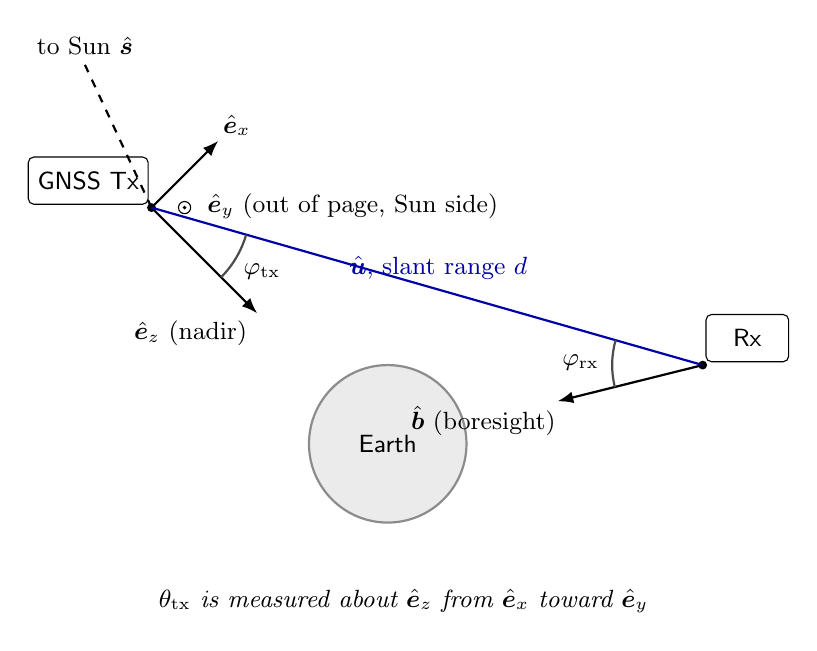
\begin{tikzpicture}[>=Latex, scale=1.0]
    % --- central body ---
    \fill[black!8] (0,0) circle (1.0);
    \draw[thick, black!45] (0,0) circle (1.0);
    \node[font=\small\sffamily] at (0,0) {Earth};

    % --- transmitter and receiver ---
    \coordinate (TX) at (-3,3);
    \coordinate (RX) at (4,1);
    \node[tsnode, above left=1pt and 1pt of TX] {GNSS Tx};
    \node[tsnode, above right=1pt and 1pt of RX] {Rx};
    \fill (TX) circle (1.6pt);
    \fill (RX) circle (1.6pt);

    % --- body triad at the transmitter ---
    \draw[flow] (TX) -- ++(-45:1.9)
      node[pos=1.0, below left=-1pt and 0pt, font=\small]
      {$\uvec{e}_z$ (nadir)};
    \draw[flow] (TX) -- ++(45:1.2)
      node[pos=1.0, above right=-2pt and -2pt, font=\small] {$\uvec{e}_x$};
    \draw[fill=white] (TX) ++(0.42,0.0) circle (2.2pt);
    \fill (TX) ++(0.42,0.0) circle (0.7pt);
    \node[font=\small, right=1pt] at ($(TX)+(0.55,0.02)$)
      {$\uvec{e}_y$ (out of page, Sun side)};

    % --- Sun direction ---
    \draw[table] (TX) -- ++(115:2.0)
      node[pos=1.0, above, font=\small] {to Sun $\uvec{s}$};

    % --- line of sight ---
    \draw[linear] (TX) -- (RX)
      node[pos=0.52, above, font=\small] {$\uvec{u}$, slant range $d$};

    % --- off-boresight angle at the transmitter ---
    \draw[thick, black!70] ($(TX)+(-45:1.25)$) arc (-45:-16:1.25);
    \node[font=\small] at ($(TX)+(-30:1.62)$) {$\varphi_\mathrm{tx}$};

    % --- receiver boresight ---
    \draw[flow] (RX) -- ++(194:1.9)
      node[pos=1.0, below left=-2pt and -3pt, font=\small]
      {$\uvec{b}$ (boresight)};
    \draw[thick, black!70] ($(RX)+(164:1.15)$) arc (164:194:1.15);
    \node[font=\small] at ($(RX)+(179:1.55)$) {$\varphi_\mathrm{rx}$};

    % --- azimuth reminder ---
    \node[font=\small\itshape, align=center] at (0.2,-2.0)
      {$\theta_\mathrm{tx}$ is measured about $\uvec{e}_z$ from
       $\uvec{e}_x$ toward $\uvec{e}_y$};
  \end{tikzpicture}
  \caption{Transmit and receive antenna geometry.  The transmitter body triad
  $(\uvec{e}_x,\uvec{e}_y,\uvec{e}_z)$ is nadir-pointing with
  $\uvec{e}_y$ orthogonal to the satellite-Sun-Earth plane; the transmit gain
  is sampled at the off-boresight angle $\varphi_\mathrm{tx}$ and azimuth
  $\theta_\mathrm{tx}$ of the line of sight $\uvec{u}$, and the receive gain at
  the angle $\varphi_\mathrm{rx}$ between the receive boresight $\uvec{b}$ and
  the reversed line of sight.}
  \label{fig:lb-geometry}
\end{figure}

\begin{lstlisting}[language=cpp, caption={Boresight-angle extraction and gain
lookup inside the $C/N_0$ computation.}, label={lst:lb-computecn0}]
// cpp/lupnt/measurements/gnss_measurement.cc :: GNSSMeasurements::ComputeCN0
Vec3 r_boresight_target_eci = BoresightTarget(receive_time);
Vec3 u_rx2body = (r_boresight_target_eci - r_rx_eci).normalized();

Real t_tdb = ConvertGnssEpoch(receive_time, options_.receive_time_scale,
                              Time::TDB);
Vec6 rv_tx_gcrf = ConvertFrame(t_tdb, rv_tx, options_.frame, Frame::GCRF);
Vec3 r_rx_gcrf  = ConvertFrame(t_tdb, r_rx_eci, options_.frame, Frame::GCRF);
Vec3 r_sun_gcrf = ConvertFrame(t_tdb, SunPosition(receive_time),
                               options_.frame, Frame::GCRF);
Vec3 u_tx2rx_gcrf = (r_rx_gcrf - rv_tx_gcrf.head(3)).normalized();

Vec3 ex, ey, ez;
GnssAttitude::Compute(rv_tx_gcrf.head(3), Vec3(rv_tx_gcrf.tail(3)),
                      r_sun_gcrf, ex, ey, ez);
Real phi_tx   = safe_acos(u_tx2rx_gcrf.dot(ez));
Real theta_tx = atan2(u_tx2rx_gcrf.dot(ey), u_tx2rx_gcrf.dot(ex));
Real phi_rx   = safe_acos(u_rx2body.dot(u_rx2tx));

Real G_tx = constellation->GetTransmitterAntenna(channel.prn,
                                                 channel.frequency)
                .ComputeGain(theta_tx, phi_tx);
Real G_rx = rx_antenna_.ComputeGain(0.0, phi_rx);
Real P_tx = constellation->GetTransmitPowerDbw(channel.prn,
                                               channel.frequency);

return LinkBudget(P_tx, G_tx, G_rx, range, channel.frequency, rx_params_);
\end{lstlisting}

The direct Sun-vector construction of \cref{eq:lb-triad} is
\cpp{GnssAttitude::Compute(r\_sat, r\_sun, ...)}:

\begin{lstlisting}[language=cpp, caption={Direct Sun-pointing body-frame
construction.}, label={lst:lb-attitude}]
// cpp/lupnt/attitude/gnss_attitude.cc :: GnssAttitude::Compute
void GnssAttitude::Compute(const Vec3& r_sat_eci, const Vec3& r_sun_eci,
                           Vec3& ex, Vec3& ey, Vec3& ez) {
  //   ez = normalize(-r_sat)                                (nadir)
  //   ey = normalize(cross(ez, normalize(r_sun - r_sat)))   (toward Sun)
  //   ex = normalize(cross(ey, ez))                         (completes triad)
  ez = (-r_sat_eci).normalized();
  Vec3 e_to_sun = (r_sun_eci - r_sat_eci).normalized();
  ey = ez.cross(e_to_sun).normalized();
  ex = ey.cross(ez).normalized();
}
\end{lstlisting}

\section{The Nominal Yaw-Steering Law}
\label{sec:lb-yaw}

The velocity-aware overload
\cpp{GnssAttitude::Compute(r, v, r\_sun, ...)} builds the same frame through
the documented \emph{nominal yaw-steering law} of \citet{kouba2009yaw}, in the
parameterization of \citep[Eq.~(1)]{cheng2025yaw}, implemented in
\file{cpp/lupnt/attitude/gnss_yaw_steering.cc}.  This is the overload actually
called by \cpp{ComputeCN0}.

\subsection{Satellite-Sun-Earth geometry}
\label{sec:lb-yaw-geometry}

Two angles parameterize the geometry.  Let
\begin{equation}
  \uvec{n}
  = \frac{\vec{r}_\mathrm{tx} \times \vec{v}_\mathrm{tx}}
         {\lVert \vec{r}_\mathrm{tx} \times \vec{v}_\mathrm{tx} \rVert},
  \qquad
  \uvec{s} = \widehat{\vec{r}_\odot},
  \label{eq:lb-orbit-normal}
\end{equation}
be the orbit normal (angular-momentum direction) and the geocentric Sun
direction.  The \emph{Sun elevation above the orbital plane} is
\begin{equation}
  \beta = \sin^{-1}\!\big(\uvec{n}\transpose \uvec{s}\big)
  \in \left[-\tfrac{\pi}{2}, \tfrac{\pi}{2}\right],
  \label{eq:lb-beta}
\end{equation}
positive when the Sun lies on the same side of the orbital plane as
$\uvec{n}$.  The \emph{orbit angle} $\mu$ is measured in the orbital plane, in
the direction of motion, from the orbit midnight point.  With the anti-Sun
direction projected into the orbital plane,
\begin{equation}
  \vec{m} = -\uvec{s} + \big(\uvec{s}\transpose\uvec{n}\big)\,\uvec{n},
  \qquad
  \uvec{m} = \widehat{\vec{m}},
  \label{eq:lb-midnight}
\end{equation}
the signed angle from $\uvec{m}$ to the satellite radial direction
$\uvec{r} = \widehat{\vec{r}_\mathrm{tx}}$ about $\uvec{n}$ is
\begin{equation}
  \mu
  = \atantwo\!\Big(
      \big(\uvec{m} \times \uvec{r}\big)\transpose \uvec{n},\
      \uvec{m}\transpose \uvec{r}
    \Big),
  \label{eq:lb-mu}
\end{equation}
so that $\mu = 0$ at the midnight point (satellite directly behind the Earth as
seen from the Sun) and $\mu = \pm\pi$ at the noon point.  The orbit noon angle
used by the maneuver laws is $\eta = \mathrm{wrap}_\pi(\mu - \pi)$.

\subsection{Nominal yaw angle and rate}
\label{sec:lb-yaw-nominal}

The nominal yaw angle that keeps the solar-panel axis $\uvec{e}_y$
perpendicular to the satellite-Sun direction while the antenna boresight stays
nadir-pointing is
\begin{equation}
  \psi(\beta, \mu)
  = \atantwo\!\big(-\tan\beta,\ \sin\mu\big),
  \label{eq:lb-yaw-nominal}
\end{equation}
with the corresponding yaw rate obtained by differentiating
\cref{eq:lb-yaw-nominal} along the orbit,
\begin{equation}
  \dot{\psi}
  = \dot{\mu}\,
    \frac{\tan\beta\,\cos\mu}
         {\sin^{2}\!\mu + \tan^{2}\!\beta}.
  \label{eq:lb-yaw-rate}
\end{equation}

\begin{lstlisting}[language=cpp, caption={Satellite-Sun-Earth geometry and the
nominal yaw law.}, label={lst:lb-yaw}]
// cpp/lupnt/attitude/gnss_yaw_steering.cc
Real GnssYawSteering::BetaAngle(const Vec3& r_sat, const Vec3& v_sat,
                                const Vec3& r_sun) {
  Vec3 n = r_sat.cross(v_sat).normalized();  // orbit normal
  Vec3 s_hat = r_sun.normalized();
  return safe_asin(n.dot(s_hat));
}

Real GnssYawSteering::OrbitAngle(const Vec3& r_sat, const Vec3& v_sat,
                                 const Vec3& r_sun) {
  Vec3 n = r_sat.cross(v_sat).normalized();
  Vec3 s_hat = r_sun.normalized();
  Vec3 r_hat = r_sat.normalized();
  Vec3 m = -s_hat - (-s_hat).dot(n) * n;   // anti-Sun, in the orbital plane
  Vec3 m_hat = m.normalized();
  return atan2(m_hat.cross(r_hat).dot(n), m_hat.dot(r_hat));
}

// Eq. (1) of Cheng et al. (2025); Kouba (2009)
Real GnssYawSteering::NominalYawAngle(Real beta, Real mu) {
  return atan2(-tan(beta), sin(mu));
}

Real GnssYawSteering::NominalYawRate(Real beta, Real mu, Real mu_dot) {
  Real tan_beta = tan(beta);
  Real sin_mu = sin(mu);
  return mu_dot * tan_beta * cos(mu) / (sin_mu * sin_mu + tan_beta * tan_beta);
}
\end{lstlisting}

\subsection{From yaw angle to body triad}
\label{sec:lb-yaw-frame}

\cpp{GnssAttitude::ComputeFromYawAngle} rotates the orbital reference axes
about the nadir axis by $\psi$.  With
\begin{equation}
  \uvec{e}_z = \widehat{-\vec{r}_\mathrm{tx}},
  \qquad
  \uvec{e}_x^{\mathrm{ref}} = \widehat{\vec{v}_\mathrm{tx}},
  \qquad
  \uvec{e}_y^{\mathrm{ref}} = \uvec{e}_z \times \uvec{e}_x^{\mathrm{ref}},
  \label{eq:lb-orbital-ref}
\end{equation}
the body axes are
\begin{equation}
  \uvec{e}_x
  = \cos\psi\,\uvec{e}_x^{\mathrm{ref}}
  + \sin\psi\,\uvec{e}_y^{\mathrm{ref}},
  \qquad
  \uvec{e}_y
  = -\sin\psi\,\uvec{e}_x^{\mathrm{ref}}
  + \cos\psi\,\uvec{e}_y^{\mathrm{ref}}.
  \label{eq:lb-yaw-rotation}
\end{equation}
Substituting $\psi$ from \cref{eq:lb-yaw-nominal} into
\cref{eq:lb-yaw-rotation} reproduces the direct Sun-vector construction
\eqref{eq:lb-triad} exactly, because the nominal yaw law is by definition the
yaw angle that keeps the solar panels Sun-pointing; the equivalence is checked
numerically in \file{cpp/test/agents/test_gnss_attitude.cc}.

\subsection{Eclipse and noon-turn caveats}
\label{sec:lb-yaw-eclipse}

\Cref{eq:lb-yaw-nominal} is singular in rate as $\beta \to 0$: near the orbit
noon and midnight points the required yaw rate \eqref{eq:lb-yaw-rate} exceeds
the attitude-control authority of a real satellite, which then rate-limits its
slew and departs from nominal by up to $180^\circ$ for tens of minutes.
\cpp{GnssYawSteering} therefore also implements the block-specific
\emph{modeled} laws of \citet{cheng2025yaw} --- GPS~IIF shadow crossing and
noon turn (Eqs.~3--5), GPS~IIR midnight and noon turns (Eqs.~6--7), the
GPS~III and Galileo~IOV collinearity-region laws (Eqs.~8--11, 17--18), the
Galileo~FOC and BDS-3~CAST cosine-transition laws (Eqs.~12--14), and the BDS-3
SECM CSNO/MCSNO laws (Eqs.~15--16).  Each is a stateless pure function of the
geometry; the \code{TxYawModel::DEDICATED} option selects the eclipse law for
GPS and Galileo and falls back to nominal for other systems.

\begin{lupntnote}
The thesis \citep[Ch.~6.4.3]{iiyama2026thesis} assumes \emph{nominal} yaw
steering, with the antenna boresight aligned to the spacecraft-Earth direction
and the solar-panel axis orthogonal to the Earth-satellite-Sun plane;
off-nominal eclipse-season steering is listed as future work.  \lupnt{}
implements the nominal law used by \cpp{ComputeCN0} and additionally exposes
the maneuver laws as building blocks, but no maneuver-window state machine is
wired into the $C/N_0$ path: \code{TxYawModel::DEDICATED} evaluates the
eclipse law \emph{continuously} from geometry rather than on a maneuver
schedule, which is an approximation of the true eclipse-season attitude.
\end{lupntnote}

\begin{lupntwarning}
The eclipse laws matter for the link budget only through the transmit azimuth
$\theta_\mathrm{tx}$, since $\varphi_\mathrm{tx}$ is unaffected by a rotation
about $\uvec{e}_z$.  For an axisymmetric (1D) transmit pattern the yaw model
is therefore irrelevant, and the two \code{TxYawModel} settings give identical
$C/N_0$.  The distinction only becomes observable with a 2D
$G(\varphi,\theta)$ pattern.
\end{lupntwarning}

\section{Receiver Tracking-Loop Noise from $C/N_0$}
\label{sec:lb-tracking}

Once $C/N_0$ is known, the per-observable measurement standard deviations
follow from the tracking-loop thermal-noise models of \citet{kaplan2017} and
\citet{misra2011gnss}.  Throughout this section
\begin{equation}
  \gamma
  = 10^{\left(C/N_0\right)_{\mathrm{dB\text{-}Hz}}/10}
  \qquad [\si{\hertz}]
  \label{eq:lb-gamma}
\end{equation}
is the linear carrier-to-noise-density ratio, computed by
\cpp{DecibelToDecimal}.  The loop parameters are listed in
\cref{tab:lb-loop-params}.

\subsection{Code tracking (DLL)}
\label{sec:lb-dll}

\cpp{GNSSMeasurements::ComputeSigmaRange} scales the dimensionless
code-tracking jitter returned by \cpp{SigmaDll} (in chips) by the chip length
in metres, $c\,T_c$, where $T_c = 1/R_c$ is the chip period of the spreading
code (from \code{GNSS\_RC\_MAP}).  \cpp{SigmaDll} carries three correlator
regimes, distinguished by the early-late spacing $d$ relative to the
front-end bandwidth $B_\mathrm{fe} = b\,R_c$.  Writing
\begin{equation}
  \kappa \equiv \frac{1}{T_c B_\mathrm{fe}} = \frac{1}{b}
  \qquad [\text{chip}]
  \label{eq:lb-kappa}
\end{equation}
for the correlator resolution set by the front-end bandwidth, the three
branches are
\begin{equation}
  \sigma_\mathrm{DLL}^2
  =
  \begin{cases}
    \dfrac{B_n}{2\gamma}\,\kappa\,
    \left(1 + \dfrac{1}{T_n \gamma}\right),
      & d \le \kappa
        \quad \text{(narrow correlator)}, \\[3ex]
    \dfrac{B_n}{2\gamma}
    \left[
      \kappa + \dfrac{(d - \kappa)^{2}}{(\pi - 1)\,\kappa}
    \right]
    \left(1 + \dfrac{2}{T_n \gamma\,(2 - d)}\right),
      & \kappa < d < \pi\kappa, \\[3ex]
    \dfrac{B_n}{2\gamma}\, d
    \left(1 + \dfrac{2}{T_n \gamma\,(2 - d)}\right),
      & d \ge \pi\kappa
        \quad \text{(wide correlator)},
  \end{cases}
  \label{eq:lb-sigma-dll}
\end{equation}
in units of chips${}^2$, with $B_n$ the DLL one-sided noise bandwidth in
\si{\hertz}, $T_n$ the coherent integration time in \si{\second}, and $d$ the
early-late spacing in chips.  The pseudorange standard deviation is
\begin{equation}
  \sigma_P
  =
  c\,T_c\,\sigma_\mathrm{DLL},
  \qquad\text{so that}\qquad
  \sigma_P^2
  =
  (c\,T_c)^2\,
  \frac{B_n}{2\gamma}\,
  \frac{1}{B_\mathrm{fe} T_c}
  \left(1 + \frac{1}{T_n \gamma}\right)
  \label{eq:lb-sigma-range}
\end{equation}
in the narrow-correlator regime, which is the branch selected by the \lupnt{}
defaults ($d = 0.1$ chip, $b = 2$, so $\kappa = 0.5 > d$).
\Cref{eq:lb-sigma-range} matches thesis Eq.~(6.60) term for term.

\begin{lstlisting}[language=cpp, caption={DLL jitter, all three correlator
regimes.}, label={lst:lb-sigmadll}]
// cpp/lupnt/measurements/comms_utils.cc :: SigmaDll
Real SigmaDll(const DllParams& params, Real CN0_w) {
  Real B_dll = params.B_dll;
  Real T_i = params.T_i;
  Real d = params.d;
  Real Tc = params.Tc;
  Real B_fe = params.B_fe;

  Real term_1 = B_dll / (2.0 * CN0_w);
  Real term_2 = 0.0;
  Real term_3 = 1.0 + 2.0 / (T_i * CN0_w * (2.0 - d));

  Real sigma_dll_2 = 0.0;
  if (d <= 1.0 / (Tc * B_fe)) {
    term_2 = 1.0 / (Tc * B_fe);
    term_3 = 1.0 + (1.0 / (T_i * CN0_w));
    sigma_dll_2 = term_1 * term_2 * term_3;
  } else if ((PI / (Tc * B_fe) > d) && (d > 1.0 / (Tc * B_fe))) {
    term_2 = 1.0 / (Tc * B_fe)
             + Tc * B_fe / (PI - 1) * pow(d - 1.0 / (Tc * B_fe), 2);
    sigma_dll_2 = term_1 * term_2 * term_3;
  } else {
    sigma_dll_2 = term_1 * d * term_3;
  }
  return sqrt(sigma_dll_2);
}
\end{lstlisting}

\begin{lupntnote}
The \cpp{DllParams} field comments do not match the usage:
\cpp{d} is documented as ``chip duration'' but is populated from
\cpp{rx\_params\_.D}, the early-to-late correlator spacing in chips, and
\cpp{Tc} is documented as ``spread code period'' but is populated with
$1/R_c$, the chip period.  The equations above follow the \emph{usage} in
\cpp{ComputeSigmaRange}, which is the reference-consistent reading.
\end{lupntnote}

\subsection{Carrier-phase tracking (PLL)}
\label{sec:lb-pll}

\cpp{GNSSMeasurements::ComputeSigmaCarrierPhase} converts the PLL phase jitter
to a length via $\lambda/2\pi$:
\begin{equation}
  \sigma_\Phi
  =
  \frac{\lambda}{2\pi}\,\sigma_\mathrm{PLL},
  \qquad
  \sigma_\mathrm{PLL}^2
  =
  \frac{B_p}{\gamma}
  \left(1 + \frac{1}{2\,T_p\,\gamma}\right)
  \qquad [\si{\radian\squared}],
  \label{eq:lb-sigma-pll}
\end{equation}
with $B_p$ the PLL one-sided noise bandwidth in \si{\hertz} and $T_p$ the
coherent integration time in \si{\second}.  The second factor is the
squaring-loss term of a Costas discriminator.

\begin{lstlisting}[language=cpp, caption={PLL jitter and its conversion to a
carrier-phase range error.}, label={lst:lb-sigmapll}]
// cpp/lupnt/measurements/comms_utils.cc :: SigmaPll
Real SigmaPll(const PllParams& params, Real CN0_w) {
  Real B_pll = params.B_pll;
  Real T_i = params.T_i;

  Real sigma_pll_2 = B_pll / CN0_w * (1.0 + 1.0 / (2.0 * T_i * CN0_w));
  return sqrt(sigma_pll_2);
}

// cpp/lupnt/measurements/gnss_measurement.cc
//   :: GNSSMeasurements::ComputeSigmaCarrierPhase
return lambda / (2.0 * PI) * SigmaPll(params, CN0_w);
\end{lstlisting}

\begin{lupntnote}
The thesis Eq.~(6.61) writes
$\sigma_\phi^2 = \left(\lambda/2\pi\right)^2
 \left[\,\dfrac{B_p}{2\gamma}\left(1 + \dfrac{1}{2 T_p \gamma}\right)\right]$.
The \lupnt{} \cpp{SigmaPll} uses $B_p/\gamma$ --- no factor of two in the
denominator --- so the code's carrier-phase \emph{variance} is larger than the
thesis expression by exactly a factor of two, i.e.\ the standard deviation is
larger by $\sqrt{2}$.  The DLL term matches the thesis (both use
$B_n/(2\gamma)$).  This discrepancy is documented, not fixed: changing it would
silently alter every carrier-phase covariance produced by the library.  Users
comparing against thesis numbers should scale $\sigma_\Phi$ by $1/\sqrt{2}$, or
halve $B_p$.
\end{lupntnote}

\subsection{Doppler and range-rate tracking (FLL)}
\label{sec:lb-fll}

\cpp{GNSSMeasurements::ComputeSigmaRangeRate} uses a frequency-lock-loop model,
converting a frequency jitter to a range rate via $\lambda$:
\begin{equation}
  \sigma_D
  =
  \frac{\lambda}{2\pi\,T_f}
  \sqrt{\frac{4 B_f}{\gamma}\left(1 + \frac{1}{T_f\,\gamma}\right)}
  \qquad [\si{\meter\per\second}],
  \label{eq:lb-sigma-fll}
\end{equation}
with $B_f$ the FLL one-sided noise bandwidth in \si{\hertz} and $T_f$ the
coherent integration time in \si{\second}.

\begin{lstlisting}[language=cpp, caption={The inlined FLL range-rate jitter.},
label={lst:lb-sigmafll}]
// cpp/lupnt/measurements/gnss_measurement.cc
//   :: GNSSMeasurements::ComputeSigmaRangeRate
return lambda / (2.0 * PI * rx_params_.T)
       * sqrt(4.0 * rx_params_.Bf / CN0_w
              * (1.0 + 1.0 / (rx_params_.T * CN0_w)));
\end{lstlisting}

\begin{lupntnote}
\cpp{ComputeSigmaRangeRate} inlines \cref{eq:lb-sigma-fll} rather than calling
the library helper \cpp{SigmaFll} in
\file{cpp/lupnt/measurements/comms_utils.cc}.  The two are not equivalent:
\cpp{SigmaFll} evaluates
\code{4 * F\_ll * B\_fll * (1 + 1/(T\_i * CN0\_w))} --- the leading term is
\emph{not} divided by $\gamma$ --- and additionally carries the squaring-loss
factor $F \in \{1, 2\}$ that doubles below the threshold
\cpp{CN0\_F\_fll}.  Only the inlined form in \cpp{ComputeSigmaRangeRate}
reproduces the reference expression \citep{kaplan2017}; \cpp{SigmaFll} is
currently unused by the measurement path.
\end{lupntnote}

\section{Reference Parameters}
\label{sec:lb-params}

\Cref{tab:lb-rx-params} lists the \lupnt{} receiver defaults;
\cref{tab:lb-loop-params} names the loop symbols used in
\crefrange{eq:lb-sigma-dll}{eq:lb-sigma-fll}; \cref{tab:lb-thesis-cn0} and
\cref{tab:lb-thesis-eirp} give the thesis reference values against which the
implementation is validated.

\begin{table}[htbp]
  \centering
  \caption{\cpp{GnssReceiverParams} defaults
  (\code{cpp/lupnt/agents/gnss\_constellation.h}).}
  \label{tab:lb-rx-params}
  \begin{tabular}{l l S l}
    \toprule
    Field & Symbol & {Default} & Unit / meaning \\
    \midrule
    \cpp{Bp}    & $B_p$              & 1.0    & \si{\hertz}, carrier (PLL) loop noise bandwidth \\
    \cpp{T}     & $T_p = T_n = T_f$  & 0.020  & \si{\second}, coherent integration time \\
    \cpp{b}     & $b$                & 2.0    & --, front-end bandwidth factor, $B_\mathrm{fe} = b R_c$ \\
    \cpp{Bn}    & $B_n$              & 0.7    & \si{\hertz}, code (DLL) loop noise bandwidth \\
    \cpp{Bf}    & $B_f$              & 0.2    & \si{\hertz}, frequency (FLL) loop noise bandwidth \\
    \cpp{D}     & $d$                & 0.1    & chip, early-to-late correlator spacing \\
    \cpp{L\_ad} & $L_\mathrm{ad}$    & 0.6    & \si{\dB}, A/D and implementation loss \\
    \cpp{L\_pol}& $L_\mathrm{pol}$   & 1.0    & \si{\dB}, polarization loss \\
    \cpp{L\_atm}& $L_\mathrm{atm}$   & 0.0    & \si{\dB}, atmospheric loss \\
    \cpp{T\_eff}& $T_\mathrm{eff}$   & 167.98 & \si{\kelvin}, effective noise temperature \\
    \bottomrule
  \end{tabular}
\end{table}

\begin{table}[htbp]
  \centering
  \caption{Tracking-loop symbols and the \cpp{DllParams} / \cpp{PllParams} /
  \cpp{FllParams} fields that carry them.}
  \label{tab:lb-loop-params}
  \begin{tabularx}{\textwidth}{l l l L}
    \toprule
    Symbol & Unit & Field & Meaning \\
    \midrule
    $\gamma$          & \si{\hertz} & \cpp{CN0\_w} &
      Linear carrier-to-noise density, $10^{(C/N_0)/10}$. \\
    $B_n$             & \si{\hertz} & \cpp{DllParams::B\_dll} &
      DLL one-sided noise bandwidth. \\
    $T_n$             & \si{\second}& \cpp{DllParams::T\_i} &
      DLL coherent integration time. \\
    $d$               & chip        & \cpp{DllParams::d} &
      Early-to-late correlator spacing. \\
    $T_c$             & \si{\second}& \cpp{DllParams::Tc} &
      Chip period, $1/R_c$. \\
    $B_\mathrm{fe}$   & \si{\hertz} & \cpp{DllParams::B\_fe} &
      Double-sided front-end bandwidth, $b R_c$. \\
    $B_p$             & \si{\hertz} & \cpp{PllParams::B\_pll} &
      PLL one-sided noise bandwidth. \\
    $T_p$             & \si{\second}& \cpp{PllParams::T\_i} &
      PLL coherent integration time. \\
    $B_f$             & \si{\hertz} & \cpp{FllParams::B\_fll} &
      FLL one-sided noise bandwidth. \\
    $T_f$             & \si{\second}& \cpp{FllParams::T\_i} &
      FLL coherent integration time. \\
    \bottomrule
  \end{tabularx}
\end{table}

\begin{table}[htbp]
  \centering
  \caption{Reference $C/N_0$ link-budget parameters, thesis Table~6.3
  \citep[Ch.~6.4.3]{iiyama2026thesis}, for a lunar receiver tracking
  terrestrial GPS.}
  \label{tab:lb-thesis-cn0}
  \begin{tabular}{l l l}
    \toprule
    Quantity & Symbol & Value \\
    \midrule
    GPS transmit power        & $P_\mathrm{tx}$      & \SIrange{16}{19}{\dBW} \\
    Receive antenna gain      & $G_\mathrm{rx}$      & \SI{14}{\dBi} \\
    System noise temperature  & $T_\mathrm{sys}$     & \SI{162}{\kelvin} \\
    Polarization loss         & $L_\mathrm{pol}$     & \SI{1.0}{\dB} \\
    Implementation loss       & $R_\mathrm{loss}$    & \SI{0.9}{\dB} \\
    \bottomrule
  \end{tabular}
\end{table}

\begin{table}[htbp]
  \centering
  \caption{Reference EIRP-sizing parameters, thesis Table~3.6
  \citep[Ch.~3.3]{iiyama2026thesis}, for the lunar augmented navigation
  service signal of \citep{lunanet2022}.}
  \label{tab:lb-thesis-eirp}
  \begin{tabular}{l l l}
    \toprule
    Quantity & Symbol & Value \\
    \midrule
    Carrier frequency             & $f$              & \SI{2492.028}{\mega\hertz} \\
    Required received power       & $P_\mathrm{rx}$  & $-160$ / $-147$ \si{\dBW} \\
    User receive antenna gain     & $G_\mathrm{rx}$  & \SI{3.0}{\dBi} \\
    \bottomrule
  \end{tabular}
\end{table}

The two received-power floors in \cref{tab:lb-thesis-eirp} correspond to the
weak-signal (acquisition-limited, omnidirectional user) and strong-signal
(data-demodulation) cases of the service specification; the resulting required
EIRP follows from \cref{eq:lb-eirp-required}.

\section{Model Boundaries}
\label{sec:lb-boundaries}

\begin{itemize}[leftmargin=1.4em]
  \item \textbf{Visibility.}  Occulting bodies are spheres and the test is a
        per-body pass/fail.  There is no atmospheric refraction, no
        tropospheric or ionospheric ducting of grazing rays, and no terrain
        horizon beyond the scalar elevation mask of
        \cref{eq:lb-elevation}.  Lunar topography, which can raise or lower the
        local horizon by several kilometres, is not represented.
  \item \textbf{Static loss terms.}  The $C/N_0$ budget is per-channel and
        static in $L_\mathrm{atm}$, $L_\mathrm{ad}$, $L_\mathrm{pol}$ and
        $T_\mathrm{eff}$: only $L_\mathrm{fs}$ and the two antenna gains vary
        with geometry.  In particular $T_\mathrm{eff}$ does not increase when
        the receive beam sweeps across the warm lunar surface or the Earth
        disc, and \cref{eq:lb-teff} is never evaluated internally.
  \item \textbf{Pointing.}  Only the deterministic geometric off-boresight loss
        is modelled, through the pattern lookups; attitude-control jitter and
        antenna phase-centre variation are not included in
        \cref{eq:lb-cn0}.  Phase-centre offsets are handled separately by the
        ANTEX machinery, in a different (non-orthonormal) frame.
  \item \textbf{Transmit attitude.}  The transmit gain uses the \emph{nominal}
        yaw-steering attitude \eqref{eq:lb-yaw-nominal}.  Maneuver-law
        attitudes exist in \cpp{GnssYawSteering} and can be selected with
        \code{TxYawModel::DEDICATED}, but they are evaluated continuously from
        geometry rather than gated by a maneuver-window state machine, and
        they affect only $\theta_\mathrm{tx}$ (see
        \cref{sec:lb-yaw-eclipse}).
  \item \textbf{Pattern coverage.}  A direction beyond \code{phi\_max\_}
        returns \code{NaN} rather than an extrapolated sidelobe level; the
        effective sidelobe cutoff is therefore a property of the data file, not
        of the model.  Link-budget studies that depend on far-sidelobe energy
        must supply patterns tabulated out to the required $\varphi$.
  \item \textbf{Tracking-loop noise.}  Only thermal noise is modelled.
        Dynamic stress error, oscillator phase noise, Allan-variance-driven
        jitter and vibration-induced jitter --- all of which appear in the full
        error budgets of \citet{kaplan2017} --- are omitted.  The PLL noise
        coefficient differs from the thesis by a factor of two in variance (see
        \cref{sec:lb-pll}); the DLL and the inlined FLL forms match their
        reference expressions, while the standalone \cpp{SigmaFll} helper does
        not (see \cref{sec:lb-fll}).
  \item \textbf{Multipath and interference.}  No multipath, no near-far
        interference from other GNSS signals, and no jamming or RFI margin are
        represented anywhere in \cref{eq:lb-cn0}.
\end{itemize}

\chapter{Ionosphere, Plasmasphere, and Ray Tracing}
\label{chap:ionosphere}

This chapter specifies the ionospheric and plasmaspheric group-delay model that
\lupnt{} applies to terrestrial GNSS signals received by cislunar and lunar
users.  A lunar receiver observes the terrestrial GNSS constellation through the
side lobes of the transmit antennas, so the useful links graze the Earth: the
line of sight passes almost tangentially through the topside ionosphere and then
runs for tens of Earth radii through the plasmasphere.  Neither the thin-shell
mapping of the classical GNSS literature nor the Klobuchar broadcast model is applicable
to such geometry, because both assume a single, steeply inclined crossing of a
compressed ionospheric shell \citep{misra2011gnss}.  \lupnt{} instead integrates
the electron density along the numerically ray-traced, bent signal path.

The model is specified in \citep{iiyama2026gcpm}, with the earlier conference
treatment in \citep{iiyama2025iono} and the full characterization in
\citep[Ch.~5]{iiyama2026thesis}; equation numbers of the form~(5.x) quoted below
refer to that chapter.  The implementation lives in the \code{pecsim} namespace
under \file{cpp/lupnt/environment/plasma/}:

\begin{itemize}[nosep]
  \item \file{tec/raytrace.h}, \file{tec/raytrace.cc} --- the tracer proper
        (\cpp{pecsim::trace\_ray}, \cpp{RayTraceConfig}, \cpp{PathProfile});
  \item \file{gcpm/gcpm_interface.h}, \file{gcpm/gcpm_interface.cc} --- the
        Global Core Plasma Model (GCPM) v2.4 electron density
        \citep{gallagher2000gcpm};
  \item \file{gcpm/iri_interface.h}, \file{gcpm/iri_interface.cc} --- the
        International Reference Ionosphere (IRI) submodel
        \citep{bilitza2022iri} and its solar-index options;
  \item \file{igrf/igrf_interface.h}, \file{igrf/igrf_interface.cc} --- the
        IGRF-14 geomagnetic field \citep{alken2021igrf};
  \item \file{tec/iono_model.h} --- the \cpp{IonoModel} backend selector;
  \item \file{tec/raytrace_wrapper.h}, \file{tec/raytrace_wrapper.cc} --- the
        batch driver used by the precompute path;
  \item \file{tec/neldermead.h}, \file{tec/neldermead.cc} --- the simplex solver
        used by the receiver-side convergence iteration.
\end{itemize}

The delay is consumed by the GNSS measurement model through
\cpp{GNSSMeasurements::\allowbreak ComputeIonosphere\allowbreak PlasmaRayTraceDelay}
(\file{cpp/lupnt/measurements/gnss_measurement.cc}), where it appears as
$\Delta\rho_\mathrm{plasma}$ in \cref{chap:gnss-measurements}.

\section{Scope, Units, and the Frame Contract}
\label{sec:iono-contract}

The tracer is a self-contained module with its own unit system, inherited from
the Fortran heritage of GCPM and IRI.  Every caller is responsible for
converting at the boundary.

\begin{lupntnote}
The entire plasma module is \textbf{km-based}.  The positions \code{x1},
\code{x2} passed to \cpp{trace\_ray} are in kilometres, the step size, gradient
step and cutoff radius are in kilometres, the Earth radius is
$R_E = \SI{6371.0}{\kilo\meter}$ and the speed of light is
$c = \SI{299792.458}{\kilo\meter\per\second}$
(\file{cpp/lupnt/environment/plasma/core/constants.h}).  Electron density is
evaluated internally in \si{\per\cubic\centi\meter} by GCPM and converted to
\si{\per\cubic\meter} before entering the delay integrals; one TEC unit is
$\SI{1}{\TECU} = \num{1e16}$ electrons per \si{\square\meter}.  Delays are
returned in \textbf{metres}.  SI callers such as \cpp{GNSSMeasurements} divide
their metre positions by $1000$ before calling \cpp{trace\_ray}, and use the
returned metres directly.
\end{lupntnote}

The tracer works in a geocentric, Earth-fixed Cartesian frame.  The GNSS
coupling converts the receiver and transmitter states from \code{options.frame}
into \code{raytrace\_frame} (default \code{Frame::ECEF}) and supplies an epoch in
\code{raytrace\_epoch\_scale} (default \code{Time::UTC}) expressed as seconds
from J2000:
%
\begin{equation}
  \label{eq:iono-inputs}
  \vec{x}_1 = \vec{r}_\mathrm{tx}^{\,\mathrm{ecef}}\,[\si{\kilo\meter}],
  \qquad
  \vec{x}_2 = \vec{r}_\mathrm{rx}^{\,\mathrm{ecef}}\,[\si{\kilo\meter}],
  \qquad
  t = t_\mathrm{rx}^{\UTC}\ \text{(s since J2000)} .
\end{equation}
%
The unit conversion applied to every density sample is
%
\begin{equation}
  \label{eq:iono-ne-units}
  n_e\,[\si{\per\cubic\meter}] = 10^{6}\, n_e\,[\si{\per\cubic\centi\meter}] ,
  \qquad
  \mathrm{TEC}\,[\si{\TECU}] = 10^{-16} \int_\Gamma n_e\,\dd s\,[\si{\per\square\meter}] .
\end{equation}
%
Because the arc length $s$ is carried in kilometres while $n_e$ is in
\si{\per\cubic\meter}, every path integrand in \cref{sec:iono-refractive}
carries an explicit factor $1000$ in the code.

\Cref{tab:iono-symbols} fixes the symbols used throughout the chapter.

\begin{table}[htbp]
  \centering
  \caption{Symbols used in the ionosphere/plasmasphere model.}
  \label{tab:iono-symbols}
  \small
  \begin{tabularx}{\textwidth}{llL}
    \toprule
    Symbol & Unit & Meaning \\
    \midrule
    $n_e$              & \si{\per\cubic\meter}   & Electron number density (GCPM output, converted from \si{\per\cubic\centi\meter}) \\
    $f$                & \si{\hertz}             & Carrier frequency of the link (\code{config.freq\_Hz}) \\
    $f_p$              & \si{\hertz}             & Electron plasma frequency, \cref{eq:iono-fp} \\
    $f_g$              & \si{\hertz}             & Electron gyro (cyclotron) frequency, \cref{eq:iono-fp} \\
    $\vec{B}$, $B$     & \si{\nano\tesla}        & Geomagnetic field vector and its magnitude (IGRF-14) \\
    $\theta$           & rad                     & Angle between $\vec{B}$ and the local ray direction $\uvec{s}$ \\
    $n$, $n_\mathrm{gr}$ & ---                   & Phase and group refractive indices \\
    $\Gamma$           & ---                     & The (bent) ray path from transmitter to receiver \\
    $s$                & \si{\kilo\meter}        & Arc length along $\Gamma$ \\
    $\uvec{s}$         & ---                     & Unit tangent to $\Gamma$ \\
    $\rho$             & \si{\kilo\meter}        & Straight-line (chord) distance $\lVert\vec{x}_2-\vec{x}_1\rVert$ \\
    $s_f$              & \si{\kilo\meter}        & Total traced arc length (\code{PathProfile::sf}) \\
    $r$                & \si{\kilo\meter} or $R_E$ & Geocentric radius (in $R_E$ when passed to GCPM) \\
    $K_p$              & ---                     & Planetary geomagnetic activity index (\code{config.kp}) \\
    $R_{12}$           & ---                     & 12-month running mean sunspot number (\code{config.rz12}) \\
    $F_{10.7}$         & sfu                     & Solar radio flux at \SI{10.7}{\centi\meter} \\
    $IG_{12}$          & ---                     & Ionospheric (effective) global index used by IRI for $f_oF_2$ \\
    $\mathrm{MLT}$     & h                       & Solar-magnetic local time \\
    $\phi_\mathrm{SM}$ & rad                     & Solar-magnetic latitude \\
    \bottomrule
  \end{tabularx}
\end{table}

\section{Solar-Magnetic Coordinates}
\label{sec:iono-sm}

GCPM is parameterized in solar-magnetic (SM) coordinates: $\uvec{z}_\mathrm{SM}$
is aligned with the geomagnetic dipole axis, $\uvec{x}_\mathrm{SM}$ lies in the
plane spanned by the dipole axis and the Earth--Sun line (tilted towards the
Sun), and $\uvec{y}_\mathrm{SM}$ completes the right-handed triad.  SM is the
natural frame for the plasmasphere because the cold-plasma distribution is
organized by dipole $L$-shells and by local time relative to the Sun.

The conversion is a chain of four elementary rotations
(\file{cpp/lupnt/environment/plasma/gcpm/conversions.cc}), applied to the
Earth-fixed (geographic, \code{GEO} $\equiv$ ITRF/ECEF) input position:
%
\begin{equation}
  \label{eq:iono-sm-chain}
  \vec{x}_\mathrm{SM}
  = \mat{T}_4\,\mat{T}_3\,\mat{T}_2\,\mat{T}_1^{-1}\,\vec{x}_\mathrm{GEO},
  \qquad
  \underbrace{\mathrm{GEO}}_{\text{ITRF}}
  \xrightarrow{\ \mat{T}_1^{-1}\ } \underbrace{\mathrm{GEI}}_{\text{GCRF}}
  \xrightarrow{\ \mat{T}_2\ } \mathrm{GSE}
  \xrightarrow{\ \mat{T}_3\ } \mathrm{GSM}
  \xrightarrow{\ \mat{T}_4\ } \mathrm{SM} .
\end{equation}
%
With the passive elementary rotations
%
\begin{equation}
  \mat{R}_x(\alpha) =
  \begin{bmatrix} 1 & 0 & 0 \\ 0 & \cos\alpha & \sin\alpha \\ 0 & -\sin\alpha & \cos\alpha \end{bmatrix},
  \quad
  \mat{R}_y(\alpha) =
  \begin{bmatrix} \cos\alpha & 0 & \sin\alpha \\ 0 & 1 & 0 \\ -\sin\alpha & 0 & \cos\alpha \end{bmatrix},
  \quad
  \mat{R}_z(\alpha) =
  \begin{bmatrix} \cos\alpha & \sin\alpha & 0 \\ -\sin\alpha & \cos\alpha & 0 \\ 0 & 0 & 1 \end{bmatrix},
\end{equation}
%
the four stages are as follows.  Let $T_0 = (\mathrm{MJD} - 51544.5)/36525$ be
the time in Julian centuries from J2000 and let $\mathrm{ut}$ be the UT hour of
day.

\paragraph{Stage 1 (GEI $\leftrightarrow$ GEO).}  A rotation about the polar
axis by the Greenwich mean sidereal angle,
%
\begin{equation}
  \label{eq:iono-t1}
  \mat{T}_1 = \mat{R}_z(\vartheta),
  \qquad
  \vartheta = \left(100.461 + 36000.770\,T_0 + 15.04107\,\mathrm{ut}\right)^{\circ} .
\end{equation}
%
The tracer applies $\mat{T}_1^{-1} = \mat{R}_z(-\vartheta)$ to lift the ECEF
input into the quasi-inertial GEI frame.

\paragraph{Stage 2 (GEI $\to$ GSE).}  A rotation into the ecliptic and then to
the Sun direction,
%
\begin{equation}
  \label{eq:iono-t2}
  \mat{T}_2 = \mat{R}_z(\lambda_\odot)\,\mat{R}_x(\varepsilon),
\end{equation}
%
with obliquity, mean anomaly, mean longitude and apparent solar longitude
%
\begin{align}
  \varepsilon    &= \left(23.439 - 0.013\,T_0\right)^{\circ}, \\
  M              &= \left(357.528 + 35999.05\,T_0 + 0.04107\,\mathrm{ut}\right)^{\circ}, \\
  \gamma         &= \left(280.46 + 36000.772\,T_0 + 0.04107\,\mathrm{ut}\right)^{\circ}, \\
  \lambda_\odot  &= \gamma + \left(1.915 - 0.0048\,T_0\right)^{\circ}\sin M
                    + 0.020^{\circ}\sin 2M .
\end{align}

\paragraph{Stages 3 and 4 (GSE $\to$ GSM $\to$ SM).}  Let $\vec{q}$ be the
geomagnetic dipole unit vector expressed in GSE.  It is built from the IGRF
dipole pole in geographic coordinates and rotated forward through stages~1
and~2:
%
\begin{equation}
  \label{eq:iono-dipole}
  \phi_\mathrm{dip} = \left(78.8 + \num{4.283e-2}\,F\right)^{\circ},
  \qquad
  \lambda_\mathrm{dip} = \left(289.1 - \num{1.413e-2}\,F\right)^{\circ},
  \qquad
  F = \frac{\mathrm{MJD} - 46066}{365.25} ,
\end{equation}
%
so that $\vec{q}_\mathrm{GEO}$ is the unit vector at latitude
$\phi_\mathrm{dip}$ and longitude $\lambda_\mathrm{dip}$, and
$\vec{q} = \mat{T}_2\mat{T}_1^{-1}\vec{q}_\mathrm{GEO}$.  Then
%
\begin{equation}
  \label{eq:iono-t3t4}
  \mat{T}_3 = \mat{R}_x(\psi), \quad \psi = -\arctan\!\left(\frac{q_y}{q_z}\right),
  \qquad
  \mat{T}_4 = \mat{R}_y(\mu), \quad
  \mu = -\arctan\!\left(\frac{q_x}{\sqrt{q_y^2+q_z^2}}\right) .
\end{equation}
%
$\mat{T}_3$ rolls the frame about the Earth--Sun line until the dipole axis lies
in the $x$--$z$ plane (giving GSM); $\mat{T}_4$ pitches by the dipole tilt angle
$\mu$ until $\uvec{z}$ coincides with the dipole axis (giving SM).  When $q_z=0$
the code substitutes $\psi = -\tfrac{\pi}{2}\operatorname{sign}(q_y)$.

\paragraph{Spherical parameters passed to GCPM.}  After the rotation the
Cartesian SM position is converted to spherical coordinates and to magnetic
local time:
%
\begin{equation}
  \label{eq:iono-mlt}
  r = \frac{\lVert\vec{x}_\mathrm{SM}\rVert}{R_E},
  \qquad
  \phi_\mathrm{SM} = \arctan\!\left(\frac{z_\mathrm{SM}}{\sqrt{x_\mathrm{SM}^2 + y_\mathrm{SM}^2}}\right),
  \qquad
  \mathrm{MLT} = 12 + \frac{12}{\pi}\,\lambda_\mathrm{SM}\ \ [\mathrm{h}],
\end{equation}
%
where $\lambda_\mathrm{SM} = \atantwo(y_\mathrm{SM}, x_\mathrm{SM})$ is wrapped
into $[0,2\pi)$ and $\mathrm{MLT}$ is reduced modulo \SI{24}{\hour}.  Noon
($\mathrm{MLT}=12$) therefore corresponds to $\lambda_\mathrm{SM}=0$, i.e.\ the
sunward side of the SM frame.

\begin{lstlisting}[language=cpp, caption={Solar-magnetic transformation and GCPM
call.  Source: \texttt{cpp/lupnt/environment/plasma/tec/raytrace.cc} ::
\code{compute\_ne}.}, label={lst:iono-computene}]
// cpp/lupnt/environment/plasma/tec/raytrace.cc :: compute_ne
double compute_ne(double t_j2000, const Vec3d& pos_geo, RayTraceConfig config, bool debug) {
  double kp = config.kp;                       // Kp index for the ionosphere model
  if (kp < 0) throw std::runtime_error("Kp index is not set. Please set the Kp index.");
  if (get_iri_model() == IRIModel::NONE)
    throw std::runtime_error("IRI model is not set. Please set the IRI model.");

  double alatr = 0.0, along = 0.0, r = 0.0;
  std::array<double, 3> pos_gei_arr = {pos_geo[0] / RE, pos_geo[1] / RE, pos_geo[2] / RE};
  std::array<double, 3> pos_sm;

  double mjd = tj2000_to_mjd(t_j2000);
  DateTime datetime = mjd_to_datetime(mjd);
  std::array<int, 2> itime = datetime_to_itime(datetime);

  geo_to_sm(itime, pos_gei_arr, pos_sm);       // GEO -> GEI -> GSE -> GSM -> SM
  cart_to_pol(pos_sm, alatr, along, r);        // r in RE, alatr in rad, along in [0, 2pi)
  double amlt = 12.0 + along / AMLTRAD;        // magnetic local time [hours]
  if (amlt > 24.0) amlt -= 24.0;

  std::vector<double> out;
  if (config.use_fortran_gcpm) out = gcpm_v24_fortran(datetime, r, amlt, alatr, kp);
  else                         out = gcpm_v24(datetime, r, amlt, alatr, kp);
  return out[0];                               // total electron density [cm^-3]
}
\end{lstlisting}

\begin{lupntnote}
The local variable is named \code{pos\_gei\_arr}, but the routine invoked is
\cpp{geo\_to\_sm}: the argument is interpreted as an Earth-fixed (GEO/ITRF)
position, consistent with \code{raytrace\_frame} defaulting to
\code{Frame::ECEF}.  The name is a historical artefact and does not indicate a
frame change.  Note also that \cref{eq:iono-t1,eq:iono-t2} are the low-precision
sidereal and solar series used by the GCPM support code; they carry
milliarcsecond-class errors that are irrelevant at the resolution of an
empirical plasma model, but they are \emph{not} the IAU~2006/2000A chain used
elsewhere in \lupnt{} (\cref{chap:frame-conversions}).
\end{lupntnote}

\section{Electron-Density Environment: GCPM v2.4 over IRI}
\label{sec:iono-density}

The electron density is supplied by the Global Core Plasma Model (GCPM) v2.4
\citep{gallagher2000gcpm}, an empirical model of the cold plasma of the inner
magnetosphere.  GCPM stitches together region-specific submodels --- the
ionosphere (delegated to IRI \citep{bilitza2022iri}), the plasmasphere, the
plasmapause, the mid-latitude trough, and the polar cap --- using
hyperbolic-tangent blending functions so that the composite density field is
continuous and differentiable, which is a prerequisite for the gradient-driven
ray tracing of \cref{sec:iono-eikonal}.

As a mathematical contract the density along the path is
%
\begin{equation}
  \label{eq:iono-ne-model}
  n_e = n_e\big(r,\ \phi_\mathrm{SM},\ \mathrm{MLT};\ K_p,\ R_{12},\ t\big) ,
\end{equation}
%
with the spatial arguments defined by \cref{eq:iono-mlt} and the remaining
arguments defined below.

\subsection{Region blending}
\label{sec:iono-blending}

Let $L = r/\cos^2\phi_\mathrm{SM}$ be the dipole $L$-shell of the sample point
(clamped by $\cos^2\phi_\mathrm{SM}\ge 10^{-5}$), and let $L_\mathrm{crit}$ be the
$L$-shell of the poleward edge of the auroral oval, obtained by bilinear
interpolation of the empirical table $P_N$ / $P_S$ in $(\mathrm{MLT},K_p)$.  The
transition half-width is $\Delta L = 2.0$.  GCPM uses the switching function
%
\begin{equation}
  \label{eq:iono-switchon}
  \sigma(L; L_\mathrm{crit}, \Delta L)
  = \frac{1}{2}\left[1 + \tanh\!\left(\frac{3.4534\,(L - L_\mathrm{crit})}{\Delta L}\right)\right] ,
\end{equation}
%
which rises from $0$ to $1$ to within \SI{0.1}{\percent} as $L$ crosses
$L_\mathrm{crit} \pm \Delta L$, and blends the plasmasphere/trough branch with
the polar-cap branch:
%
\begin{equation}
  \label{eq:iono-blend}
  n_e =
  \begin{cases}
    n_e^\mathrm{ps/trough}, & L < L_\mathrm{crit} - \Delta L, \\[4pt]
    (1-\sigma)\,n_e^\mathrm{ps/trough} + \sigma\,n_e^\mathrm{cap},
      & L_\mathrm{crit} - \Delta L \le L \le L_\mathrm{crit} + \Delta L, \\[4pt]
    n_e^\mathrm{cap}, & L > L_\mathrm{crit} + \Delta L .
  \end{cases}
\end{equation}
%
Both branches call IRI below the F2 peak and bridge smoothly to the
plasmaspheric/polar profiles above it.  The same $\sigma$ controls the ion
composition: with $h = (r-1)R_E$ the altitude in \si{\kilo\meter},
%
\begin{align}
  \label{eq:iono-composition}
  \frac{n_{\mathrm{He}^+}}{n_{\mathrm{H}^+}}
    &= 10^{\,-1.541 - 0.176\,r + \num{8.557e-3}F_{10.7} - \num{1.458e-5}F_{10.7}^2}
       \left[1 - \sigma(L; L_\mathrm{crit}, \Delta L)\right], \\
  \alpha_{\mathrm{O}^+}
    &= \frac{0.995}{\left[1 + \left(\dfrac{h - 350}{531.25}\right)^{2}\right]^{3}} + 0.005 ,
\end{align}
%
from which the $\mathrm{H}^+$, $\mathrm{He}^+$ and $\mathrm{O}^+$ partial
densities are recovered.
Only the \emph{total} electron density (output slot~0) enters the delay
integrals; the ion partition is carried for diagnostics.

\begin{lstlisting}[language=cpp, caption={GCPM v2.4 region blending.  Source:
\texttt{cpp/lupnt/environment/plasma/gcpm/gcpm\_interface.cc} ::
\code{gcpm\_v24}.}, label={lst:iono-gcpm}]
// cpp/lupnt/environment/plasma/gcpm/gcpm_interface.cc :: gcpm_v24
IRIParams params = iri_sm(0.0, 0.0, 1.01, itime);   // f107 / rz12 / hmF2 from IRI
double f107 = params.f107, rz12 = params.rz12, hmf2_km = params.hmf2_km;

alcrit   = 1.0 / pow(cos(alatcritn * DEG2RAD), 2);  // L-shell of the auroral edge
tranlow  = alcrit - altrans;                        // altrans = 2.0
tranhigh = alcrit + altrans;

clat = pow(cos(alatr), 2);
if (clat < 1.0e-5) clat = 1.0e-5;
al      = r / clat;                                 // dipole L-shell
aheight = (r - 1.0) * re;                           // altitude [km]

double edensity = 0.0;
if (al < tranlow) {
  edensity = ne_iri_ps_trough(r, al, alatr, amlt, akp, itime);
} else if (al <= tranhigh) {
  double ps_edensity  = ne_iri_ps_trough(r, al, alatr, amlt, akp, itime);
  double cap_edensity = ne_iri_cap(r, alatr, amlt, itime);
  double switch_val   = switchon(al, alcrit, altrans);
  edensity = ps_edensity * (1.0 - switch_val) + cap_edensity * switch_val;
} else {
  edensity = ne_iri_cap(r, alatr, amlt, itime);
}
double den = edensity / 1.0e6;                      // -> particles per cm^3
\end{lstlisting}

\subsection{Model inputs}
\label{sec:iono-inputs}

\begin{description}[style=nextline, leftmargin=1.2em]
  \item[$K_p$ --- \code{config.kp}]
    The planetary geomagnetic activity index.  It sets the plasmapause radius:
    higher $K_p$ erodes the plasmasphere, contracting the plasmapause from
    $\sim$4--6\,$R_E$ under quiet conditions to $\sim$2--3\,$R_E$ under active
    conditions, and it also drives the auroral-edge table that fixes
    $L_\mathrm{crit}$ in \cref{eq:iono-switchon}.  \cpp{compute\_ne} throws when
    $K_p < 0$.  Passing $K_p<0$ directly to \cpp{gcpm\_v24} instead triggers a
    lookup of the historical index for the requested epoch.
  \item[$R_{12}$ --- \code{config.rz12}]
    The 12-month running mean sunspot number, which parameterizes the IRI
    submodel.  See \cref{sec:iono-indices}.
  \item[$t$ --- the epoch]
    Sets both the IRI solar-activity state and the SM frame orientation through
    \cref{eq:iono-t1,eq:iono-t2,eq:iono-t3t4}.
\end{description}

\begin{lupntnote}
\code{config.kp} must be non-negative and an IRI model must have been selected
with \cpp{set\_iri\_model} --- \cpp{compute\_ne} throws otherwise.  GCPM and IRI
describe only the inner-magnetospheric cold plasma; contributions beyond the
cutoff radius (default $4\,R_E$, see \cref{sec:iono-eikonal}) are neglected,
where the densities are orders of magnitude lower and the residual delay is well
below the noise floor of a lunar GNSS receiver.
\end{lupntnote}

\begin{lupntwarning}
GCPM cannot be evaluated for arbitrary future epochs: it requires historical
solar and geomagnetic indices, and the bundled \file{apf107.dat} and
\file{ig_rz.dat} tables end around 2024 with only a short projection.  Both
\cpp{iri\_sm} and \cpp{gcpm\_v24\_fortran} therefore step the requested year
backwards (up to 30 times) until the solar-index tables have coverage, so a
future epoch silently falls back to the most recent available activity rather
than returning NaN.  The thesis baseline sidesteps this by using
2025-01-01 12:00 UTC as an explicit proxy epoch for a 2027 scenario and by
sweeping $K_p \in \{1, 3, 5, 6.667, 9\}$ and
$R_{12} \in \{10, 50, 100, 150, 200\}$ \citep[Ch.~5]{iiyama2026thesis}.
\end{lupntwarning}

\section{Solar Indices: \texorpdfstring{$R_{12}$}{R12}, \texorpdfstring{$F_{10.7}$}{F10.7} and \texorpdfstring{$IG_{12}$}{IG12}}
\label{sec:iono-indices}

IRI is driven by three correlated solar indices.  When the user supplies a
sunspot number $R_{12}$ directly, \lupnt{} derives the other two from it with
the PHaRLAP relations \citep{cervera2014pharlap}, which are the same polynomial
fits used inside the IRI Fortran core (thesis Eqs.~5.19--5.20):
%
\begin{align}
  \label{eq:iono-f107}
  F_{10.7} &= 63.75 + 0.728\,R_{12} + \num{0.00089}\,R_{12}^2 , \\
  \label{eq:iono-ig12}
  IG_{12}  &= -12.349154 + 1.4683266\,R_{12} - \num{0.00267690893}\,R_{12}^2 .
\end{align}
%
$F_{10.7}$ (the \SI{10.7}{\centi\meter} solar radio flux, in solar flux units)
drives the topside and composition models; $IG_{12}$ is the
ionospheric-effective index used by IRI for the F2 critical frequency $f_oF_2$.
The derived triple is written into the IRI output array \code{oarr} at the
Fortran slots for $R_{12}$, $IG_{12}$ and $F_{10.7}$ before the model call, and
IRI2020 additionally receives $F_{10.7,81} = F_{10.7}$.

\begin{lstlisting}[language=cpp, caption={PHaRLAP solar-index relations and the
IRI user-input path.  Source:
\texttt{cpp/lupnt/environment/plasma/gcpm/iri\_interface.cc} ::
\code{iri\_sub}.}, label={lst:iono-indices}]
// cpp/lupnt/environment/plasma/gcpm/iri_interface.cc :: iri_sub  (IRI 2020 branch)
R12 = iri_option_2020.R12;
if (R12 > 0.0) {
  f107 = 63.75 + R12 * (0.728 + R12 * 0.00089);
  IG12 = -12.349154 + R12 * (1.4683266 - R12 * 2.67690893e-03);
  *(oarr + 32) = static_cast<float>(R12);
  *(oarr + 38) = static_cast<float>(IG12);
  *(oarr + 40) = static_cast<float>(f107);
  *(oarr + 45) = static_cast<float>(f107);   /* F10.7_81 is set to F10.7 */
}
iri_sub_2020_(iri_option_2020.jf2020, &jmag, &blatdf, &blongdf, &yyyy, &mddd,
              &dhourf, &aheight1f, &aheight2f, &delhf, outf, oarr);
\end{lstlisting}

The sign of \code{config.rz12} selects between user-supplied and
historical/projected indices following the IRI convention, and simultaneously
switches the foF2 storm model.  \cpp{trace\_ray} pushes \code{config.rz12} into
the active option object (\cpp{IRI2007Option} or \cpp{IRI2020Option}) and
re-derives the Fortran logical-flag array \code{jf} before tracing.

\begin{table}[htbp]
  \centering
  \caption{Interpretation of \code{RayTraceConfig::rz12} and the resulting IRI
  Fortran flags.  Flag indices are one-based, as in the IRI documentation.}
  \label{tab:iono-rz12}
  \small
  \begin{tabularx}{\textwidth}{lLl}
    \toprule
    \code{rz12} & Meaning & IRI flags \\
    \midrule
    $0 < R_{12} \le 200$ & User-supplied sunspot number; $F_{10.7}$ and $IG_{12}$ derived from \cref{eq:iono-f107,eq:iono-ig12} & \code{jf(17)}, \code{jf(25)}, \code{jf(27)}, \code{jf(32)} $=$ false; storm model off \\
    $-1$ & IRI historical / projected $R_{12}$, storm model on & all four $=$ true; \code{jf(26)} $=$ true \\
    $-2$ & IRI historical / projected $R_{12}$, storm model off (IRI2007 only) & \code{jf(26)} $=$ false \\
    other & Rejected --- \cpp{update\_jf\_2007} / \cpp{update\_jf\_2020} throws \code{"Invalid value for R12"} & --- \\
    \bottomrule
  \end{tabularx}
\end{table}

\section{GCPM Interpolation Surrogate}
\label{sec:iono-gcpm-surrogate}

GCPM is expensive because each call
performs $\sim$10 IRI evaluations.  For bulk work --- Monte-Carlo delay budgets,
data-assimilation experiments --- \lupnt{} provides an optional interpolation
surrogate (\code{RayTraceConfig::use\_gcpm\_surrogate}, default off;
\file{gcpm/gcpm\_surrogate.h}, \file{gcpm/gcpm\_surrogate.cc}).  GCPM's \emph{own}
output is pre-sampled on a seven-dimensional grid in its natural solar-magnetic
frame plus UT,
%
\begin{equation}
  \label{eq:iono-gcpm-surrogate}
  n_e = f\big(r,\ \phi_\mathrm{SM},\ \mathrm{MLT},\ \mathrm{UT},\ K_p,\ R_{12},\ \mathrm{doy}\big),
\end{equation}
%
stored as $\log n_e$ and interpolated multilinearly (with MLT/UT/season periodic),
so the model's plasmapause and region-blending logic are baked in.  It is used as a
\emph{hybrid}: above $r = 1.15\,R_E$, where GCPM is plasmasphere-organized and
interpolates cleanly, the table is queried; below it, where the sharp,
\emph{geographic} F-region is not representable on a solar-magnetic grid, the call
falls through to full GCPM.  The surrogate is
exact at grid nodes, gives a $\sim$2\% median error on ray-integrated lunar-link
delays, and is $14$--$200\times$ faster than full GCPM per call --- always more
than $10\times$.

\begin{lupntwarning}
The GCPM surrogate does \emph{not} reach sub-percent accuracy, and no practical
grid can: in solar-magnetic coordinates the ionosphere's geographic structure
(solar zenith, terminator, equatorial anomaly) becomes razor-sharp, and the
ionosphere--plasmasphere bridge keeps GCPM universal-time-dependent up to
$\sim$1.6\,$R_E$ at mid/high latitude.  A genuinely sub-percent fast GCPM would
require re-deriving a smooth parametric emulator ($N_{mF_2}$, $h_{mF_2}$, and scale
heights reconstructed into a Chapman profile).  Use the surrogate where a $\sim$2\% delay error
is acceptable in exchange for the speedup; leave it off for reference evaluations.
\end{lupntwarning}

\section{Geomagnetic Field: IGRF-14}
\label{sec:iono-igrf}

The magnetic field is required only by the second- and third-order delay terms
of \cref{sec:iono-refractive}.  \lupnt{} evaluates it with the IGRF-14
coefficient set \citep{alken2021igrf}, whose scalar potential is the truncated
spherical-harmonic series
%
\begin{equation}
  \label{eq:iono-igrf-potential}
  V(r,\vartheta,\lambda,t)
  = a \sum_{n=1}^{N} \sum_{m=0}^{n}
    \left(\frac{a}{r}\right)^{n+1}
    \Big[ g_n^m(t)\cos m\lambda + h_n^m(t)\sin m\lambda \Big]\,
    P_n^m(\cos\vartheta) ,
\end{equation}
%
where $a = \SI{6371.2}{\kilo\meter}$ is the IGRF reference radius,
$\vartheta$ is geocentric colatitude, $\lambda$ is east longitude, $P_n^m$ are
Schmidt quasi-normalized associated Legendre functions, $N = 13$ for the main
field, and the Gauss coefficients are linearly interpolated between five-year
epochs with a secular-variation extrapolation beyond the last epoch,
%
\begin{equation}
  g_n^m(t) = g_n^m(T_k) + (t - T_k)\,\dot{g}_n^m ,
\end{equation}
%
with $t$ the decimal year.  The local north/east/down (NEC) components follow
from $\vec{B} = -\nabla V$ as
%
\begin{equation}
  \label{eq:iono-bfield}
  X = \frac{1}{r}\frac{\partial V}{\partial \vartheta},
  \qquad
  Y = -\frac{1}{r\sin\vartheta}\frac{\partial V}{\partial \lambda},
  \qquad
  Z = \frac{\partial V}{\partial r},
  \qquad
  B = \sqrt{X^2 + Y^2 + Z^2} \ \ [\si{\nano\tesla}] .
\end{equation}
%
The projection of the field on the ray enters the delay through
%
\begin{equation}
  \label{eq:iono-costheta}
  \cos\theta = \frac{\vec{B}\cdot\uvec{s}}{B} ,
\end{equation}
%
i.e.\ the cosine of the angle between the local field line and the local
propagation direction.  The decimal year handed to the Fortran routine is
$t = \mathrm{year} + (\mathrm{doy}-1)/365.25$.

\begin{lstlisting}[language=cpp, caption={IGRF-14 evaluation and the ray/field
angle.  Sources: \texttt{cpp/lupnt/environment/plasma/igrf/igrf\_interface.cc} and
\texttt{cpp/lupnt/environment/plasma/tec/raytrace.cc} ::
\code{compute\_B}.}, label={lst:iono-igrf}]
// cpp/lupnt/environment/plasma/igrf/igrf_interface.cc :: igrf14
std::vector<double> igrf14(double lat_rad, double lon_rad, double r_km, double decimal_year) {
  int isv = 0;               // 0 = main field, not secular variation
  int itype = 2;             // 1 = geodetic, 2 = geocentric
  double x, y, z, f;
  double colat_deg = 90.0 - lat_rad * 180.0 / M_PI;
  double elong_deg = lon_rad * 180.0 / M_PI;
  if (elong_deg < 0) elong_deg += 360.0;
  igrf14syn_(&isv, &decimal_year, &itype, &r_km, &colat_deg, &elong_deg, &x, &y, &z, &f);
  return {x, y, z};          // north, east, vertical [nT]
}

// cpp/lupnt/environment/plasma/tec/raytrace.cc :: compute_B
cart_to_pol(pos_geo_arr, lat_rad, lon_rad, r);
double decimal_year = datetime.year + (datetime.doy - 1) / 365.25;
std::vector<double> B = igrf14(lat_rad, lon_rad, r, decimal_year);   // [nT]

// cpp/lupnt/environment/plasma/tec/raytrace.cc :: ray_derivative
Vec3d B_vec = compute_B(t_epoch, x, config, debug);   // in nT
double B_dot_s = B_vec.dot(s_hat);
B         = B_vec.norm();                             // in nT
cos_theta = B_dot_s / B;
\end{lstlisting}

\begin{lupntnote}
The delay coefficients hard-coded in \file{raytrace.cc} assume $B$ in
\textbf{nanotesla}, whereas the thesis writes the symbolic coefficients for $B$
in tesla.  This is the sole source of the numerical difference between the two
sets of constants; see \cref{tab:iono-coeffs}.
\end{lupntnote}

\begin{lupntwarning}
\cpp{igrf14} returns the field in the local north/east/vertical triad, but
\cpp{ray\_derivative} dots that triple directly with $\uvec{s}$, which is
expressed in geocentric Cartesian components.  The magnitude $B$ is unaffected
(it is frame-invariant), so the $n_e B^2(1+\cos^2\theta)$ part of the third-order
term is bounded correctly, but $\cos\theta$ as computed mixes the two triads and
is therefore only an order-of-magnitude proxy for the true field/ray angle.  The
terms affected are $d_{I2}$ and the $\cos^2\theta$ part of $d_{I3}$, which the
lunar characterization places several orders of magnitude below $d_{I1}$ and
which the GNSS default (\code{TEC\_ONLY}, \cref{sec:iono-gnss}) omits entirely.
Enable \code{compute\_higher\_order} for magnitude studies, not for
sub-centimetre error budgets.
\end{lupntwarning}

\section{Refractive Index, Group Delay, and TEC}
\label{sec:iono-refractive}

\subsection{Appleton--Hartree}
\label{sec:iono-appleton}

For a cold, magnetized, collisional plasma the complex phase refractive index of
a characteristic magnetoionic mode is given by the Appleton--Hartree relation
\citep{budden1985}
%
\begin{equation}
  \label{eq:iono-ah}
  n^2 = 1 -
  \frac{X}{\,1 - \mathrm{i}Z - \dfrac{Y_T^2}{2\,(1 - X - \mathrm{i}Z)}
        \pm \sqrt{\dfrac{Y_T^4}{4\,(1 - X - \mathrm{i}Z)^2} + Y_L^2}\,} ,
\end{equation}
%
with the dimensionless parameters
%
\begin{equation}
  \label{eq:iono-xyz}
  X = \frac{f_p^2}{f^2}, \qquad
  Y = \frac{f_g}{f}, \qquad
  Y_L = Y\cos\theta, \qquad
  Y_T = Y\sin\theta, \qquad
  Z = \frac{\nu}{2\pi f} ,
\end{equation}
%
where $\nu$ is the electron collision frequency.  The characteristic frequencies
are
%
\begin{equation}
  \label{eq:iono-fp}
  f_p^2 = \frac{n_e e^2}{4\pi^2 \epsilon_0 m_e} \approx 80.6\, n_e
  \ \ [\si{\square\hertz}] ,
  \qquad
  f_g = \frac{e B}{2\pi m_e} \approx 28\,B
  \ \ [\si{\hertz},\ B\ \text{in}\ \si{\nano\tesla}] ,
\end{equation}
%
with $e$ the elementary charge, $m_e$ the electron mass and $\epsilon_0$ the
vacuum permittivity.  The upper sign selects the ordinary mode and the lower
sign the extraordinary mode; a right-hand circularly polarized GNSS signal
propagating in the northern magnetic hemisphere follows the branch for which the
$f_g\cos\theta$ term appears with the sign written below.

At GNSS frequencies the ionosphere is weakly refracting and effectively
collisionless: $X \lesssim 10^{-4}$, $Y \lesssim 10^{-3}$ and $Z \approx 0$ above
the D region.  \lupnt{} therefore uses the quasi-longitudinal series expansion of
\cref{eq:iono-ah} truncated after the $f^{-4}$ term (thesis Eqs.~5.1--5.2):
%
\begin{align}
  \label{eq:iono-phase-index}
  n &= 1
     - \frac{f_p^2}{2f^2}
     - \frac{f_p^2 f_g \cos\theta}{2f^3}
     - \frac{f_p^2}{4f^4}\!\left[\frac{f_p^2}{2} + f_g^2\left(1+\cos^2\theta\right)\right] , \\[4pt]
  \label{eq:iono-group-index}
  n_\mathrm{gr} &= 1
     + \frac{f_p^2}{2f^2}
     + \frac{f_p^2 f_g \cos\theta}{f^3}
     + \frac{3f_p^2}{4f^4}\!\left[\frac{f_p^2}{2} + f_g^2\left(1+\cos^2\theta\right)\right] .
\end{align}
%
The group index follows from the phase index through
$n_\mathrm{gr} = \dd(fn)/\dd f$, which is what produces the factors
$1 \to 2 \to 3$ on the successive orders.  The delay is dispersive, scaling as
$f^{-2}$ at leading order; this is what makes the dual-frequency
ionosphere-free combination of \cref{chap:gnss-measurements} possible.

\subsection{Group delay along the path}
\label{sec:iono-groupdelay}

Integrating $n_\mathrm{gr}-1$ along the ray gives the excess group path (thesis
Eqs.~5.4--5.7):
%
\begin{equation}
  \label{eq:iono-delay-orders}
  d_{I_\mathrm{gr}} = \int_\Gamma \left(n_\mathrm{gr}-1\right)\dd s
    = \frac{p}{f^2} + \frac{q}{f^3} + \frac{u}{f^4} ,
\end{equation}
%
with, in SI units and $B$ in tesla,
%
\begin{align}
  \label{eq:iono-p}
  p &= 40.3 \int_\Gamma n_e\,\dd s
     = 40.3\,\mathrm{TEC}
     = 40.3\left(\mathrm{TEC}_\mathrm{LOS} + \Delta\mathrm{TEC}_\mathrm{bend}\right) , \\
  \label{eq:iono-q}
  q &= -\num{2.2566e12} \int_\Gamma n_e\, B \cos\theta\,\dd s , \\
  \label{eq:iono-u}
  u &= 2437 \int_\Gamma n_e^2\,\dd s
     + \num{4.74e22} \int_\Gamma n_e\, B^2 \left(1+\cos^2\theta\right)\dd s .
\end{align}
%
The first-order coefficient is $40.3 = \tfrac{1}{2}\cdot 80.6$ and carries units
of \si{\meter\cubed\per\square\second}; the second-order coefficient is
$\num{2.2566e12} = 7527\,c$, the familiar higher-order ionospheric constant of
the GNSS literature.  The integral of $n_e$ along the path is the total electron
content,
%
\begin{equation}
  \label{eq:iono-tecu}
  \mathrm{TEC} = \int_\Gamma n_e\,\dd s\ \ [\si{\per\square\meter}],
  \qquad
  \SI{1}{\TECU} = \num{1e16}\,\si{\per\square\meter},
  \qquad
  \SI{1}{\TECU} \ \Longrightarrow\ \SI{0.162}{\meter}\ \text{at L1} .
\end{equation}
%
Because $\Gamma$ is curved, the TEC splits into a line-of-sight part
$\mathrm{TEC}_\mathrm{LOS}$, obtained by sampling the same density field along
the straight chord, and a bending increment
$\Delta\mathrm{TEC}_\mathrm{bend} = \mathrm{TEC} - \mathrm{TEC}_\mathrm{LOS}$.
For terrestrial and LEO users the second- and third-order terms remain below
about \SI{1}{\percent} of the first order; for the grazing lunar geometry the
characterization of \citep[Tab.~5.2]{iiyama2026thesis} finds them several orders
of magnitude below $d_{I1}$.

\subsection{Sign conventions}
\label{sec:iono-signs}

Three sign conventions must be kept apart.

\begin{enumerate}[nosep]
  \item \textbf{Phase versus group.}  $n < 1$ and $n_\mathrm{gr} > 1$: the code
        observable is \emph{delayed} and the carrier phase is \emph{advanced} by
        the same first-order amount.  \cref{eq:iono-delay-orders} is the group
        (code) delay and is positive.
  \item \textbf{The stored $q$.}  The code accumulates $q$ with a
        \emph{positive} coefficient \code{q\_coeff}.  The physical sign is
        carried by $\cos\theta$ (which changes sign when the ray reverses
        relative to the field) and, in the phase index, by the explicit minus in
        $n = 1 - (p/f^2 + q/2f^3 + u/3f^4)$.  The thesis instead absorbs the sign
        into the symbolic definition of $q$ in Eq.~(5.6), hence the leading minus
        in \cref{eq:iono-q}.
  \item \textbf{Phase versus group factors.}  The phase index uses
        $q/(2f^3)$ and $u/(3f^4)$; the group-delay accumulators use $q/f^3$ and
        $u/f^4$.  Both are consistent with
        \cref{eq:iono-phase-index,eq:iono-group-index} --- the group form simply
        omits the $\tfrac{1}{2}$ and $\tfrac{1}{3}$ phase factors.
\end{enumerate}

\begin{lstlisting}[language=cpp, caption={Phase index used to bend the ray, and
the three group-delay accumulators.  Source:
\texttt{cpp/lupnt/environment/plasma/tec/raytrace.cc} ::
\code{refractive\_index\_neB}, \code{ray\_derivative}.}, label={lst:iono-index}]
// cpp/lupnt/environment/plasma/tec/raytrace.cc
static const double p_coeff  = 40.3;     // first-order
static const double q_coeff  = 2.2566e3; // second-order  (for B in nT)
static const double u1_coeff = 2437;     // third-order, ne^2 part
static const double u2_coeff = 4.74e4;   // third-order, B^2 part (for B in nT)

// :: refractive_index_neB  -- the phase index that bends the ray
double p = p_coeff * ne_m3;
double q = 0.0, u = 0.0;
if (compute_q) {
  q = q_coeff * ne_m3 * B * cos_theta;
  u = u1_coeff * ne_m3 * ne_m3 + u2_coeff * ne_m3 * B * B * (1 + cos_theta * cos_theta);
}
double n = 1 - (p / f2 + q / (2 * f3) + u / (3 * f4));   // phase refractive index

// :: ray_derivative -- per-arc group-delay accumulators (s is in km, hence *1000)
dz(7) = ne_m3 * 1000;                                  // d(TEC)/ds       [m^-2 per km]
dz(8) = q_coeff * ne_m3 * B * cos_theta * 1000;        // second-order integrand
dz(9) = 1000 * (u1_coeff * ne_m3 * ne_m3
              + u2_coeff * ne_m3 * B * B * (1 + cos_theta * cos_theta));  // third order
\end{lstlisting}

\begin{table}[htbp]
  \centering
  \caption{Delay coefficients: code constants (with $B$ in \si{\nano\tesla})
  versus the SI symbolic values of \citep[Ch.~5]{iiyama2026thesis} (with $B$ in
  \si{\tesla}).}
  \label{tab:iono-coeffs}
  \small
  \begin{tabular}{llll}
    \toprule
    Term & Code constant & Value ($B$ in \si{\nano\tesla}) & SI value ($B$ in \si{\tesla}) \\
    \midrule
    $p$, first order      & \code{p\_coeff}  & $40.3$          & $40.3$ \\
    $q$, second order     & \code{q\_coeff}  & $\num{2.2566e3}$ & $\num{2.2566e12}$ \quad ($\times 10^{-9}$) \\
    $u$, third order, $n_e^2$ & \code{u1\_coeff} & $2437$      & $2437$ \\
    $u$, third order, $B^2$   & \code{u2\_coeff} & $\num{4.74e4}$ & $\num{4.74e22}$ \quad ($\times 10^{-18}$) \\
    \bottomrule
  \end{tabular}
\end{table}

\section{Vector Eikonal Ray Tracing}
\label{sec:iono-eikonal}

\subsection{Governing equations and state}
\label{sec:iono-state}

In the geometric-optics limit the signal path obeys the vector eikonal (ray)
equations, integrated with respect to arc length $s$ (thesis Eqs.~5.11--5.13):
%
\begin{equation}
  \label{eq:iono-eikonal}
  \frac{\dd t}{\dd s} = \frac{n}{c},
  \qquad
  \frac{\dd \vec{r}}{\dd s} = \uvec{s},
  \qquad
  \frac{\dd \uvec{s}}{\dd s}
    = \frac{\nabla n - \uvec{s}\,(\uvec{s}\cdot\nabla n)}{n} ,
\end{equation}
%
subject to the two-point boundary conditions
$\vec{r}(t_\mathrm{tx}) = \vec{r}_\mathrm{tx}$ and
$\vec{r}(t_\mathrm{rx}) = \vec{r}_\mathrm{rx}$.  The right-hand side of the third
equation is the component of $\nabla n$ perpendicular to the ray, normalized by
$n$: the ray bends towards increasing refractive index, and the parallel
component --- which would only rescale $\lVert\uvec{s}\rVert$ --- is projected
out, keeping $\uvec{s}$ on the unit sphere.

The integrated state has ten components,
%
\begin{equation}
  \label{eq:iono-statevec}
  \vec{z} = \big[\,\underbrace{\vec{r}}_{0..2},\ \underbrace{\uvec{s}}_{3..5},\
                  \underbrace{\Delta t}_{6},\ \underbrace{\mathrm{TEC}}_{7},\
                  \underbrace{I_2}_{8},\ \underbrace{I_3}_{9}\,\big]
       \in \mathbb{R}^{10},
\end{equation}
%
where $\Delta t = t - t_\mathrm{tx}$ and $I_2$, $I_3$ are the second- and
third-order delay integrals of \cref{eq:iono-q,eq:iono-u} (without the $f^{-3}$,
$f^{-4}$ factors, which are applied once at the end).  The refractive-index
gradient is a central finite difference with step \code{config.gradn\_dx}
(default \SI{1}{\kilo\meter}):
%
\begin{equation}
  \label{eq:iono-gradn}
  \left[\nabla n\right]_i
  = \frac{n(\vec{x} + \delta\,\uvec{e}_i) - n(\vec{x} - \delta\,\uvec{e}_i)}{2\delta},
  \qquad i = 1,2,3, \qquad \delta = \code{gradn\_dx} .
\end{equation}
%
Each gradient evaluation therefore costs six GCPM calls, which dominates the
runtime and motivates both the stored-gradient reuse of
\cref{sec:iono-correction} and the batch precompute path of
\cref{sec:iono-precompute}.

\begin{lstlisting}[language=cpp, caption={Eikonal right-hand side.  Source:
\texttt{cpp/lupnt/environment/plasma/tec/raytrace.cc} ::
\code{ray\_derivative}.}, label={lst:iono-derivative}]
// cpp/lupnt/environment/plasma/tec/raytrace.cc :: ray_derivative
Vec3d dshat_ds = Vec3d::Zero();
if (config.straight_ray) dshat_ds.setZero();
else                     dshat_ds = (grad_n - s_hat * grad_n.dot(s_hat)) / n;   // Eq. (5.13)

VecXd dz(STATE_SIZE);
dz.segment<3>(0) = s_hat;      // dr/ds   = s_hat
dz.segment<3>(3) = dshat_ds;   // ds_hat/ds
// We only track the time increase due to distance here due to machine precision
// in tracking TEC delays (= p_coeff * ne_m3 / (freq_Hz * freq_Hz) / C = ne_m3 * 1e-23)
// -> We do not want to keep epochs and TEC delays in the same vector
dz(6) = 1.0 / C;               // dt/ds  ~ 1/c (vacuum; the plasma delay is added later)
\end{lstlisting}

\begin{lupntnote}
The geometric propagation time is accumulated as $\dd t/\dd s = 1/c$ (vacuum)
rather than $n/c$, and the plasma contribution is added once at the end as
$(d_{I1} + d_{I2} + d_{I3})/c$.  This is a deliberate floating-point choice: the
per-step TEC time increment is of order $n_e \cdot 10^{-23}\,\si{\second}$, far
below the resolution of a double holding an epoch of order $10^{8}\,\si{\second}$
from J2000, so co-accumulating the two would lose the delay entirely.  The result
is algebraically identical to integrating $\dd t/\dd s = n/c$.
\end{lupntnote}

\subsection{Integration and the adaptive step schedule}
\label{sec:iono-integration}

\code{config.integ\_method} selects between the explicit Euler step
%
\begin{equation}
  \label{eq:iono-euler}
  \vec{z}_{k+1} = \vec{z}_k + h\,\vec{F}(s_k, \vec{z}_k),
  \qquad s_{k+1} = s_k + h ,
\end{equation}
%
and the classical fourth-order Runge--Kutta step \citep{hairer1993}
%
\begin{equation}
  \label{eq:iono-rk4}
  \begin{gathered}
    \vec{k}_1 = \vec{F}(s_k, \vec{z}_k), \qquad
    \vec{k}_2 = \vec{F}\!\left(s_k + \tfrac{h}{2},\ \vec{z}_k + \tfrac{h}{2}\vec{k}_1\right), \\
    \vec{k}_3 = \vec{F}\!\left(s_k + \tfrac{h}{2},\ \vec{z}_k + \tfrac{h}{2}\vec{k}_2\right), \qquad
    \vec{k}_4 = \vec{F}\!\left(s_k + h,\ \vec{z}_k + h\,\vec{k}_3\right), \\
    \vec{z}_{k+1} = \vec{z}_k
      + \frac{h}{6}\left(\vec{k}_1 + 2\vec{k}_2 + 2\vec{k}_3 + \vec{k}_4\right) .
  \end{gathered}
\end{equation}
%
RK4 costs four density/gradient evaluations per step (i.e.\ 28 GCPM calls with
the finite-difference gradient) and correspondingly quadruples the storage
width; Euler is the default because the adaptive schedule below already keeps
the local truncation error well inside the model error of GCPM itself.  After
each step $\uvec{s}$ is renormalized, which removes the drift that the
projection in \cref{eq:iono-eikonal} leaves at $O(h^2)$.

The step size is not error-controlled but keyed on altitude
$\mathrm{alt} = r - R_E$, which is an excellent proxy for the density scale
height:
%
\begin{equation}
  \label{eq:iono-step}
  h(\mathrm{alt}) =
  \begin{cases}
    \SI{10}{\kilo\meter},  & \mathrm{alt} < \SI{1000}{\kilo\meter}, \\
    \SI{20}{\kilo\meter},  & \SI{1000}{\kilo\meter} \le \mathrm{alt} < \SI{4000}{\kilo\meter}, \\
    \SI{100}{\kilo\meter}, & \mathrm{alt} \ge \SI{4000}{\kilo\meter} .
  \end{cases}
\end{equation}
%
The schedule is enabled by \code{config.use\_adaptive\_step} (default true) and
overrides \code{config.step\_size} within the plasmasphere; the final partial
step is clipped so that $s$ lands exactly on $s_f$.  Because the schedule can
reduce the step to \SI{10}{\kilo\meter} even when \code{config.step\_size} is
larger, the per-step storage matrix is allocated for the worst case
$\lceil s_f/\SI{10}{\kilo\meter}\rceil + 2$ rows and trimmed afterwards.

\begin{lstlisting}[language=cpp, caption={Altitude-keyed step schedule.  Source:
\texttt{cpp/lupnt/environment/plasma/tec/raytrace.cc} ::
\code{adjust\_stepsize}.}, label={lst:iono-step}]
// cpp/lupnt/environment/plasma/tec/raytrace.cc :: adjust_stepsize
double adjust_stepsize(double r, const VecXd& store_vec) {
  double step_size = 20.0;   // Default step size in km
  double alt = r - RE;       // Altitude in km
  if (alt < 1000)      step_size = 10.0;    // Smaller step size for closer distances
  else if (alt < 4000) step_size = 20.0;    // Default step size for medium distances
  else                 step_size = 100.0;   // Maximum step size for very far distances
  return step_size;
}
\end{lstlisting}

\subsection{Cutoff split and the terminal shot}
\label{sec:iono-cutoff}

The path is split into a plasmasphere section and a vacuum section at the cutoff
radius \code{config.cutoff\_r} (default
$4\,R_E \approx \SI{25484}{\kilo\meter}$).  Beyond the cutoff the density is
taken as zero, so $\nabla n = \vec{0}$ and the ray is exactly straight; there is
no point integrating it.  When the marching state first satisfies
$r \ge r_\mathrm{cut}$ \emph{and} $r > r_\mathrm{prev}$ (the second test prevents
an inbound ray from terminating on entry), the tracer projects the remaining
displacement onto the exit direction (thesis Eqs.~5.17--5.18):
%
\begin{equation}
  \label{eq:iono-shoot}
  \Delta s = \left(\vec{x}_\mathrm{rx} - \vec{x}_\mathrm{exit}\right)\cdot\uvec{s}_\mathrm{exit},
  \qquad
  s_f = s_\mathrm{exit} + \Delta s,
  \qquad
  \vec{x}_f = \vec{x}_\mathrm{exit} + \Delta s\,\uvec{s}_\mathrm{exit} .
\end{equation}
%
$\Delta s$ is the least-squares closest approach along the exit ray, so the
residual $\vec{x}_f - \vec{x}_\mathrm{rx}$ is exactly the component of the miss
perpendicular to $\uvec{s}_\mathrm{exit}$ --- which is precisely the quantity the
direction correction of \cref{sec:iono-correction} drives to zero.  The
propagation time is extended by the vacuum flight time $\Delta s / c$.

\begin{lstlisting}[language=cpp, caption={Cutoff exit and terminal shot.  Source:
\texttt{cpp/lupnt/environment/plasma/tec/raytrace.cc} ::
\code{propagate\_ray}.}, label={lst:iono-shoot}]
// cpp/lupnt/environment/plasma/tec/raytrace.cc :: propagate_ray
if ((r >= cutoff_r) && (r > r_prev)) {
  // Find sf that minimizes |fpos - x2|, where fpos = pos_now + dir_now * (sf - s)
  Vec3d delta_x2 = x2 - pos_now;
  double delta_s = delta_x2.dot(dir_now);
  sf = s + delta_s;
  Vec3d final_pos = pos_now + dir_now * (sf - s);
  double computed_prop_time = z(6) + (sf - s) / C;
  z.segment<3>(0) = final_pos;
  z(6) = computed_prop_time;
  cutoff_hit_p = true;
  break;
}
\end{lstlisting}

\subsection{Receiver-side convergence iteration}
\label{sec:iono-correction}

\Cref{eq:iono-eikonal} is an initial-value problem, but the physical problem is a
two-point boundary-value problem: the unknown launch direction $\uvec{s}_0$ must
be chosen so that the ray lands on the receiver.  \lupnt{} solves it by shooting.
Parameterizing the launch direction by azimuth and elevation,
$\uvec{s}_0 = \uvec{s}(\alpha, \epsilon)$, the objective is the terminal miss
distance
%
\begin{equation}
  \label{eq:iono-miss}
  J(\alpha,\epsilon)
  = \left\lVert \bar{\vec{x}}_\mathrm{rx}(\alpha,\epsilon) - \vec{x}_\mathrm{rx} \right\rVert ,
\end{equation}
%
where $\bar{\vec{x}}_\mathrm{rx}$ is the terminal position produced by
\cpp{propagate\_ray}.  The iteration is initialized with the straight-line
direction and chord length,
$\uvec{s}_0 = (\vec{x}_2 - \vec{x}_1)/\rho$ and $s_f = \rho$, and alternates two
updates for at most 20 coarse iterations:

\begin{enumerate}[nosep]
  \item \textbf{Propagation-time refresh} (\cpp{correct\_proptime}).  The
        propagation time is reset to include the plasma delay accumulated on the
        current path,
        %
        \begin{equation}
          \label{eq:iono-proptime}
          \tau \leftarrow \Delta t
            + \frac{1}{c}\left(\frac{p}{f^2} + \frac{q}{f^3} + \frac{u}{f^4}\right) ,
        \end{equation}
        %
        which in turn moves $t_\mathrm{tx} = t_\mathrm{rx} - \tau$ and hence the
        epoch at which GCPM is sampled.  This is the light-time iteration of
        thesis Eq.~(5.16), consistent with \cref{chap:gnss-measurements}.
  \item \textbf{Direction re-solve} (\cpp{correct\_dir\_neldermead}).  $J$ is
        minimized over $(\alpha, \epsilon)$ with a two-dimensional Nelder--Mead
        simplex.
\end{enumerate}

The coarse loop terminates as soon as one of
%
\begin{equation}
  \left|J_k - J_{k-1}\right| < \SI{1}{\meter},
  \qquad
  J_k > J_{k-1},
  \qquad
  J_k \le \code{corr\_tol}
\end{equation}
%
holds; if the error increased, the previous direction, state and stored
derivative matrix are restored.  To keep the cost tractable, the coarse pass
runs with \code{use\_precomputed\_vals = true}: it replays the per-step
refractive index, gradient, $n_e$, $B$ and $\cos\theta$ stored in
\code{store\_mat} on the previous propagation, together with the step sizes that
produced them, instead of re-querying GCPM at every point.  Only the geometry is
re-integrated.  The stored rows are trimmed to those actually written, so a
perturbed ray that runs longer than the reference simply stops at the last stored
row.

An optional finer pass (\code{config.fine\_correction}) re-solves with GCPM
evaluated at every step, either with Nelder--Mead again or with a
finite-difference Newton update:
%
\begin{equation}
  \label{eq:iono-newton}
  \mat{J} = \frac{\partial \bar{\vec{x}}_\mathrm{rx}}{\partial (\alpha,\epsilon)}
          \in \mathbb{R}^{3\times 2},
  \qquad
  \begin{bmatrix}\Delta\alpha \\ \Delta\epsilon\end{bmatrix}
    = \mat{J}^{+}\left(\vec{x}_\mathrm{rx} - \bar{\vec{x}}_\mathrm{rx}\right),
\end{equation}
%
where $\mat{J}$ is built by central differences with a perturbation of
$10^{-7}\,\si{\radian}$ and $\mat{J}^{+}$ is the thin-SVD pseudo-inverse (the
system is over-determined because the terminal shot of \cref{eq:iono-shoot}
already removed the along-track component).  The step is applied with unit
relaxation.  \Cref{tab:iono-neldermead} lists the simplex settings.

\begin{table}[htbp]
  \centering
  \caption{Nelder--Mead settings in \cpp{correct\_dir\_neldermead}.  $J_0$ is the
  terminal miss of the incoming solution, in \si{\kilo\meter}.}
  \label{tab:iono-neldermead}
  \small
  \begin{tabularx}{\textwidth}{lLL}
    \toprule
    Setting & Coarse pass (\code{coarse\_mode = true}) & Fine pass (\code{coarse\_mode = false}) \\
    \midrule
    Density/gradient source & replayed from \code{store\_mat} & re-evaluated from GCPM/IGRF \\
    Initial simplex edge     & $10^{-4}\,\si{\radian}$ & $10^{-6}$, $10^{-7}$ or $10^{-8}\,\si{\radian}$ for $J_0 > 0.1$, $J_0 \le 0.1$, $J_0 \le 0.01$ \\
    Simplex tolerance        & $10^{-8}$ & $10^{-4}$ \\
    Objective tolerance      & $10^{-6}\,\si{\kilo\meter}$ & \code{corr\_tol}$/1000$ \si{\kilo\meter} \\
    Iteration cap            & 200 & 50 \\
    \bottomrule
  \end{tabularx}
\end{table}

\begin{lstlisting}[language=cpp, caption={Coarse convergence loop: propagate,
refresh the propagation time, re-solve the launch direction.  Source:
\texttt{cpp/lupnt/environment/plasma/tec/raytrace.cc} ::
\code{trace\_ray}.}, label={lst:iono-traceray}]
// cpp/lupnt/environment/plasma/tec/raytrace.cc :: trace_ray
Vec3d dir = (x2 - x1).normalized();
double L  = (x2 - x1).norm();
double prop_time = L / C;     // straight-line light time as the initial guess
double sf = L;

int n_iter = 20;              // Number of iterations for coarse correction
for (int iter = 0; iter < n_iter; ++iter) {
  zf = propagate_ray(prop_time, dir, sf, x1, x2, epoch_utc_rx, config, store_mat, false);
  pos_err = (zf.segment<3>(0) - x2).norm();                      // [km]

  if ((abs(pos_err - pos_err_prev) < 1e-3) || (pos_err > pos_err_prev)
      || (pos_err <= config.corr_tol / 1000)) {
    if (pos_err > pos_err_prev) { dir = dir_prev; zf = zf_prev; store_mat = store_mat_prev; }
    break;
  }
  correct_proptime(prop_time, dir, sf, x1, x2, epoch_utc_rx, config, zf);
  pos_err_prev = pos_err; dir_prev = dir; zf_prev = zf; store_mat_prev = store_mat;
  correct_dir_neldermead(prop_time, dir, sf, x1, x2, epoch_utc_rx, config, zf, store_mat,
                         /*coarse_mode=*/true, debug_corr);
}
\end{lstlisting}

Without the correction the terminal miss is \SIrange{10}{100}{\kilo\meter} for a
grazing lunar link, purely because of bending; with it the miss is driven to the
sub-metre to \SI{100}{\meter} range, depending on whether the fine pass is
enabled.  The residual is reported in \code{PathProfile::corr\_final\_pos\_err}
and \code{PathProfile::corr\_final\_time\_err} so that a caller can reject
non-converged rays.

\begin{lupntwarning}
\code{config.correction\_method} must be \code{"neldermead"} or \code{"newton"};
\cpp{trace\_ray} throws otherwise.  The struct default is \code{"grid"}, which
\emph{would} throw, so any caller that enables \code{correction} must set this
field explicitly.  The thrown message text
(\code{"Supported methods are 'naive' and 'newton'"}) is stale with respect to
the check it accompanies.
\end{lupntwarning}

\section{Delay Decomposition}
\label{sec:iono-decomposition}

Once the corrected path has been integrated, \cpp{compute\_path\_profile}
converts the accumulators $z_7$, $z_8$, $z_9$ and the geometry into metres.  The
excess geometric path caused by bending is
%
\begin{equation}
  \label{eq:iono-dlen}
  d_\mathrm{len} = \int_\Gamma \dd s - \rho = s_f - \rho,
  \qquad
  \rho = \left\lVert \vec{r}_\mathrm{tx} - \vec{r}_\mathrm{rx} \right\rVert ,
\end{equation}
%
which is non-negative because the straight chord is the shortest path between the
endpoints.  The total group delay relative to the chord is then the sum of five
physically distinct terms (thesis Eqs.~5.8--5.10):
%
\begin{equation}
  \label{eq:iono-dtotal}
  d_\mathrm{total}
    = d_{I_\mathrm{gr}} + d_\mathrm{len}
    = \underbrace{40.3\,\mathrm{TEC}_\mathrm{LOS}}_{d_{I1,\mathrm{LOS}}}
    + \underbrace{q/f^3}_{d_{I2}}
    + \underbrace{u/f^4}_{d_{I3}}
    + \underbrace{40.3\,\Delta\mathrm{TEC}_\mathrm{bend}}_{d_{I1,B}}
    + d_\mathrm{len} .
\end{equation}
%
$d_{I1,\mathrm{LOS}}$ is what a straight-line TEC model would predict;
$d_{I1,B}$ is the additional dispersive delay incurred because the bent path
samples a different (generally denser, lower-altitude) part of the ionosphere;
$d_\mathrm{len}$ is the non-dispersive geometric lengthening.  The straight-line
reference $\mathrm{TEC}_\mathrm{LOS}$ is computed by
\cpp{compute\_tec\_straight}, which marches the same density field along the
chord with fixed steps of \code{config.step\_size} and zeroes any sample outside
the cutoff radius.

\begin{lstlisting}[language=cpp, caption={Assembly of the delay terms.  Source:
\texttt{cpp/lupnt/environment/plasma/tec/raytrace.cc} ::
\code{compute\_path\_profile}.}, label={lst:iono-profile}]
// cpp/lupnt/environment/plasma/tec/raytrace.cc :: compute_path_profile
double tec_straight = z(7);
if (config.straight_ray == false)
  tec_straight = compute_tec_straight(t_tx, initial_pos, final_pos, config);

double dist                  = (final_pos - initial_pos).norm();       // chord [km]
double tec_delay_m           = p_coeff * z(7) / freq2;                 // 40.3 * TEC_bent / f^2
double tec_delay_straight_m  = p_coeff * tec_straight / freq2;
double second_delay_m        = z(8) / freq3;
double third_delay_m         = z(9) / freq4;

double C_ms = C * 1000;                                                // [m/s]
double prop_time_total = z(6) + (tec_delay_m + second_delay_m + third_delay_m) / C_ms;

pp.dist_bend_m      = (sf - dist) * 1000;                              // excess path length [m]
pp.tec_delay_m      = tec_delay_m;
pp.tec_delay_bend_m = tec_delay_m - tec_delay_straight_m;
pp.total_delay_m    = pp.dist_bend_m + pp.tec_delay_m
                    + pp.second_delay_m + pp.third_delay_m;
pp.tecu             = z(7) / TECU;
pp.tecu_bend        = (z(7) - tec_straight) / TECU;
\end{lstlisting}

\begin{table}[htbp]
  \centering
  \caption{\cpp{PathProfile} scalar outputs and their mapping onto
  \cref{eq:iono-dtotal}.}
  \label{tab:iono-pathprofile}
  \small
  \begin{tabularx}{\textwidth}{llL}
    \toprule
    Field & Symbol & Meaning \\
    \midrule
    \code{tec\_delay\_m}      & $d_{I1,\mathrm{LOS}} + d_{I1,B}$ & First-order delay $40.3\,\mathrm{TEC}/f^2$ along the \emph{bent} path [\si{\meter}] \\
    \code{tec\_delay\_bend\_m}& $d_{I1,B}$        & Bending increment $40.3\,\Delta\mathrm{TEC}_\mathrm{bend}/f^2$ [\si{\meter}] \\
    \code{second\_delay\_m}   & $d_{I2}$          & $q/f^3$ [\si{\meter}] \\
    \code{third\_delay\_m}    & $d_{I3}$          & $u/f^4$ [\si{\meter}] \\
    \code{dist\_bend\_m}      & $d_\mathrm{len}$  & Excess geometric path $(s_f - \rho)$ [\si{\meter}] \\
    \code{total\_delay\_m}    & $d_\mathrm{total}$& Sum of the four rows above [\si{\meter}] \\
    \code{tecu}               & $\mathrm{TEC}$    & Bent-path TEC [\si{\TECU}] \\
    \code{tecu\_bend}         & $\Delta\mathrm{TEC}_\mathrm{bend}$ & Bent minus straight TEC [\si{\TECU}] \\
    \code{sf}                 & $s_f$             & Total traced arc length [\si{\kilo\meter}] \\
    \code{dist\_straight\_km} & $\rho$            & Chord length [\si{\kilo\meter}] \\
    \code{max\_sep\_line\_m}  & ---               & Maximum perpendicular separation of $\Gamma$ from the chord [\si{\meter}] \\
    \code{prop\_time\_total}  & $\tau$            & Total propagation time including plasma delay [\si{\second}] \\
    \code{corr\_final\_pos\_err} & ---            & Residual terminal miss $\bar{\vec{x}}_\mathrm{rx}-\vec{x}_\mathrm{rx}$ [\si{\kilo\meter}] \\
    \code{corr\_final\_time\_err}& ---            & Residual propagation-time inconsistency [\si{\second}] \\
    \bottomrule
  \end{tabularx}
\end{table}

The per-step arrays \code{s}, \code{r}, \code{pos\_eci}, \code{tec\_section},
\code{az\_dir}, \code{el\_dir} and \code{dist\_to\_line} carry the sampled
profile itself and are what the characterization plots of
\citep[Ch.~5]{iiyama2026thesis} are built from.

\section{Configuration Knobs}
\label{sec:iono-config}

\begin{table}[htbp]
  \centering
  \caption{\cpp{RayTraceConfig} (\texttt{cpp/lupnt/environment/plasma/tec/raytrace.h}).}
  \label{tab:iono-config}
  \small
  \begin{tabularx}{\textwidth}{llL}
    \toprule
    Field & Default & Effect \\
    \midrule
    \code{freq\_Hz}   & NaN & Carrier frequency [\si{\hertz}].  The constants \code{freq\_L1} $=\SI{1575.42}{\mega\hertz}$, \code{freq\_L2} $=\SI{1227.60}{\mega\hertz}$, \code{freq\_L5} $=\SI{1176.45}{\mega\hertz}$ are provided.  All delays scale as $f^{-2}$ at leading order, so L5 sees $\approx 1.8\times$ the L1 delay.  Must be set. \\
    \code{step\_size} & $10.0$ & Nominal integrator step [\si{\kilo\meter}]; also the fixed step of the straight-line TEC reference. \\
    \code{use\_adaptive\_step} & true & Enable the 10/20/100 \si{\kilo\meter} altitude schedule of \cref{eq:iono-step}. \\
    \code{integ\_method} & \code{"Euler"} & \code{"Euler"} or \code{"RK4"} (case-insensitive for RK4); anything else throws. \\
    \code{correction} & true & Run the bent-path launch-direction correction of \cref{sec:iono-correction}. \\
    \code{fine\_correction} & false & Run the additional fine pass with GCPM re-evaluated at every step. \\
    \code{correction\_method} & \code{"grid"} & Must be set to \code{"neldermead"} or \code{"newton"} when \code{correction} is on. \\
    \code{corr\_tol} & $1.0$ & Terminal miss tolerance [\si{\meter}]. \\
    \code{cutoff\_r} & $4R_E$ & Plasmasphere/vacuum boundary [\si{\kilo\meter}]. \\
    \code{gradn\_dx} & $1.0$ & Central-difference step for $\nabla n$ [\si{\kilo\meter}]. \\
    \code{kp} & $-1$ & Geomagnetic $K_p$; must be set $\ge 0$ or \cpp{compute\_ne} throws. \\
    \code{rz12} & $-1.0$ & Solar $R_{12}$; see \cref{tab:iono-rz12}. \\
    \code{compute\_higher\_order} & true & Include $d_{I2}$, $d_{I3}$ (requires the IGRF evaluation). \\
    \code{straight\_ray} & false & Force $\nabla n = \vec{0}$ and skip the coarse correction, producing the straight-line TEC baseline. \\
    \code{use\_fortran\_gcpm} & true & Use the Fortran GCPM v2.4 backend instead of the C++ reimplementation (GCPM backend only). \\
    \bottomrule
  \end{tabularx}
\end{table}

The electron-density backend itself is not a \cpp{RayTraceConfig} field but a
process-global selected with \cpp{set\_iono\_model},
in the same way \cpp{set\_iri\_model} selects the IRI submodel.

\section{Coupling into the GNSS Measurement Model}
\label{sec:iono-gnss}

When \code{options.apply\_ionosphere\_plasma\_delay} is true and ray-trace
options have been registered through
\cpp{SetIonospherePlasmaRayTraceOptions}, the GNSS model calls the tracer once
per link.

\begin{lstlisting}[language=cpp, caption={Per-link tracer invocation.  Source:
\texttt{cpp/lupnt/measurements/gnss\_measurement.cc} ::
\code{ComputeIonospherePlasmaRayTraceDelay}.}, label={lst:iono-gnss}]
// cpp/lupnt/measurements/gnss_measurement.cc :: ComputeIonospherePlasmaRayTraceDelay
pecsim::RayTraceConfig config = ray_opts.config;
if (ray_opts.use_channel_frequency) config.freq_Hz = GnssFrequencyHz(freq);
if (ray_opts.iri_model != pecsim::IRIModel::NONE) pecsim::set_iri_model(ray_opts.iri_model);

Real t_raytrace = ConvertGnssEpoch(receive_time, options_.receive_time_scale,
                                   ray_opts.raytrace_epoch_scale);
Real t_tdb      = ConvertGnssEpoch(receive_time, options_.receive_time_scale, Time::TDB);

Vec3 r_rx_ray = r_rx, r_tx_ray = r_tx;
if (ray_opts.raytrace_frame != options_.frame) {
  r_rx_ray = ConvertFrame(t_tdb, r_rx, options_.frame, ray_opts.raytrace_frame);
  r_tx_ray = ConvertFrame(t_tdb, r_tx, options_.frame, ray_opts.raytrace_frame);
}

pecsim::PathProfile profile = pecsim::trace_ray(
    t_raytrace.val(), ToVec3d(r_tx_ray) / 1000.0, ToVec3d(r_rx_ray) / 1000.0, config,
    ray_opts.debug_propagation, ray_opts.debug_correction);

Real delay_m = profile.tec_delay_m;
if (ray_opts.delay_mode == GnssIonospherePlasmaRayTraceDelayMode::TEC_PLUS_HIGHER_ORDER)
  delay_m += profile.second_delay_m + profile.third_delay_m;
return delay_m;
\end{lstlisting}

The returned $\Delta\rho_\mathrm{plasma}$ is a positive code delay and enters the
observation equations of \cref{chap:gnss-measurements} with opposite signs on the
two observables,
%
\begin{equation}
  \label{eq:iono-observables}
  \rho = \ldots + \Delta\rho_\mathrm{plasma} + \ldots ,
  \qquad
  \varphi = \ldots - \Delta\rho_\mathrm{plasma} + \ldots ,
\end{equation}
%
reflecting the phase advance / group delay duality of \cref{sec:iono-signs}.

The \cpp{GnssIonospherePlasmaRayTraceOptions} fields are \code{config} (the
tracer knobs of \cref{tab:iono-config}; note that \cpp{GNSSMeasurements} never
fills in $K_p$, the integrator or the step sizes --- those must come from the
caller), \code{raytrace\_frame} (default \code{ECEF}),
\code{raytrace\_epoch\_scale} (default \code{UTC}),
\code{use\_channel\_frequency} (default true, which overwrites
\code{config.freq\_Hz} with the channel frequency), \code{iri\_model}, and
\code{delay\_mode}.

\begin{lupntnote}
\code{delay\_mode} defaults to \code{TEC\_ONLY}, so the delay returned to the
measurement model is \code{profile.tec\_delay\_m} alone, i.e.\
$d_{I1,\mathrm{LOS}} + d_{I1,B}$; \code{TEC\_PLUS\_HIGHER\_ORDER} adds
$d_{I2} + d_{I3}$.  The geometric excess-path term $d_\mathrm{len}$
(\code{profile.dist\_bend\_m}) is computed and reported but is \textbf{not} added
to the pseudorange: its timing effect is already captured by the
$\Delta\mathrm{TEC}_\mathrm{bend}$ part of \code{tec\_delay\_m}, and the residual
sub-metre geometric lengthening is deliberately left out of the range equation.
\end{lupntnote}

\section{Batch Precompute}
\label{sec:iono-precompute}

Ray tracing is expensive: one GCPM call per gradient component per stage per
step per correction iteration.  Two execution paths therefore exist.

The \emph{online} path calls \cpp{trace\_ray} link-by-link inside
\cpp{GNSSMeasurements::Compute}.  The \emph{batch} path decouples the tracer from
filtering: in the staged lunar GNSS ODTS scenario, \cpp{Precompute} writes all
light-time-corrected links with zero plasma delay, a Python driver fills each
epoch/channel delay by ray tracing on a coarse cadence and interpolating to
\SI{1}{\hertz}, and \cpp{Run} merges the delay file back before forming the
observables.  The two paths agree exactly on the measurement model; see the
online/precompute equivalence discussion in \cref{chap:gnss-measurements}.

\begin{lstlisting}[language=py, caption={Batch delay generation driver.  Source:
\texttt{python/examples/ex6\_precompute.py} (writes
\texttt{precomputed\_delays.csv}).}, label={lst:iono-precompute}]
# python/examples/ex6_precompute.py
FREQ_HZ = {"L1": 1575.42e6, "L2": 1227.60e6, "L5": 1176.45e6,
           "E1": 1575.42e6, "E5a": 1176.45e6}
EARTH_RADIUS_KM = 6371.2

def _rt_params(cfg):
    """Picklable dict of RayTraceConfig attribute values, sent to each worker."""
    p = cfg.plasma
    return dict(step_size=p.raytrace_step_size_km,
                correction=p.raytrace_correction,
                fine_correction=p.raytrace_fine_correction,
                cutoff_r=p.raytrace_cutoff_radius_re * EARTH_RADIUS_KM,
                gradn_dx=p.raytrace_gradient_step_km,
                integ_method=p.raytrace_integrator,
                correction_method=p.raytrace_correction_method,
                kp=p.raytrace_kp, rz12=p.raytrace_rz12,
                use_fortran_gcpm=p.raytrace_use_fortran_gcpm,
                corr_tol=p.raytrace_correction_tolerance_m,
                compute_higher_order=p.raytrace_compute_higher_order,
                use_adaptive_step=p.raytrace_use_adaptive_step,
                straight_ray=p.raytrace_straight_ray)

def _init_worker(params):
    """Runs in each worker (fork or spawn): select the IRI model and build its RayTraceConfig."""
    global _RT_CONFIG
    pnt.set_iri_model("IRI2007")
    _RT_CONFIG = _build_rt_config(params)

def _trace_worker(task):
    """Ray-trace one link through GCPM/IRI2007 -> dict of delay columns."""
    t_utc, tx_km, rx_km, freq_hz = task
    _RT_CONFIG.freq_Hz = freq_hz
    profile = pnt.trace_ray(t_utc, tx_km, rx_km, _RT_CONFIG, False, False)
    tec_m = float(profile.tec_delay_m)
    higher_m = (float(profile.second_delay_m) + float(profile.third_delay_m)
                if _RT_CONFIG.compute_higher_order else 0.0)
    return {"tecu": float(profile.tecu),
            "tec_delay_m": tec_m,
            "second_delay_m": float(profile.second_delay_m),
            "third_delay_m": float(profile.third_delay_m),
            "ionosphere_plasma_delay_m": tec_m + higher_m}
\end{lstlisting}

Two details of the driver are load-bearing.  First, \cpp{set\_iri\_model} mutates
process-global Fortran COMMON state and reads the IRI data files, so it must be
called once per worker process in the initializer rather than per ray.  Second,
the cached delays are keyed on a fingerprint that combines the Stage-1 link
fingerprint with every \cpp{RayTraceConfig} field and the interpolation cadence,
so changing $K_p$, $R_{12}$, the integrator or the cutoff invalidates the cache
while filter tuning does not.

A pure C++ batch entry point is also exposed through
\file{cpp/lupnt/environment/plasma/tec/raytrace_wrapper.h}
(\cpp{pecsim::run\_raytrace\_batch}, \cpp{load\_raytrace\_data},
\cpp{RaytraceData}), which stores per ray the fields listed in
\cref{tab:iono-batch}.  The $K_p$ time series consumed by these runs is fetched
from GFZ Potsdam by \file{python/pylupnt/plasma/kp_loader.py} and cached under
the plasma data directory.

\begin{table}[htbp]
  \centering
  \caption{Per-ray records in \cpp{RaytraceData}
  (\texttt{raytrace\_wrapper.h}).}
  \label{tab:iono-batch}
  \small
  \begin{tabularx}{\textwidth}{lL}
    \toprule
    Field & Contents \\
    \midrule
    \code{tidxs}, \code{row\_fulls}          & Transmitter index and full-table row index \\
    \code{epoch\_utcs}                       & Reception epoch [\si{\second}] \\
    \code{tx\_positions}, \code{rx\_positions} & Endpoint positions [\si{\meter}] \\
    \code{total\_delays}                     & $d_\mathrm{total}$ [\si{\meter}] \\
    \code{tecus}                             & Bent-path TEC [\si{\TECU}] \\
    \code{tec\_delays}                       & $d_{I1,\mathrm{LOS}} + d_{I1,B}$ [\si{\meter}] \\
    \code{second\_delays}, \code{third\_delays} & $d_{I2}$, $d_{I3}$ [\si{\meter}] \\
    \code{dist\_bend\_m}                     & $d_\mathrm{len}$ [\si{\meter}] \\
    \code{tec\_delay\_bend\_m}               & $d_{I1,B}$ [\si{\meter}] \\
    \code{min\_alts}                         & Minimum (tangential) altitude along the path [\si{\meter}] \\
    \code{max\_sep\_line\_m}                 & Maximum separation from the chord [\si{\meter}] \\
    \code{final\_pos\_err\_m}                & Residual terminal miss [\si{\meter}] \\
    \bottomrule
  \end{tabularx}
\end{table}

\section{Model Boundaries and Notes}
\label{sec:iono-boundaries}

\begin{description}[style=nextline, leftmargin=1.2em]
  \item[Km-unit convention.]
    All tracer inputs and outputs are km / km-s based; SI callers scale by
    $1000$ at the boundary.  Delays, however, are returned in metres.

  \item[Magnetic-field units.]
    The delay coefficients assume $B$ in \si{\nano\tesla}; the thesis symbolic
    coefficients are the SI-tesla equivalents (\cref{tab:iono-coeffs}).  The
    field components are additionally expressed in the local north/east/down
    triad while $\uvec{s}$ is geocentric Cartesian, so $\cos\theta$ is a proxy
    rather than an exact projection.

  \item[Second and third order are small.]
    For terrestrial and LEO users they stay below about \SI{1}{\percent} of the
    first-order delay; for the lunar geometry
    \citep[Tab.~5.2]{iiyama2026thesis} places them several orders of magnitude
    below $d_{I1}$.  The GNSS default (\code{TEC\_ONLY}) omits them, and they are
    the only consumers of the IGRF evaluation.

  \item[Cutoff at $4\,R_E$.]
    Plasma outside the inner magnetosphere is neglected entirely and the path is
    taken to be exactly straight beyond the cutoff.  For a lunar receiver at
    $\approx 60\,R_E$ this means roughly \SI{93}{\percent} of the geometric path
    length contributes nothing to the delay --- which is correct to well within
    the model error, since the magnetosheath and solar-wind densities are
    $\lesssim \SI{10}{\per\cubic\centi\meter}$.

  \item[Time integration.]
    $\dd t/\dd s$ uses the vacuum $1/c$ with the plasma delay added separately;
    this is algebraically equivalent to $\dd t/\dd s = n/c$ but avoids
    catastrophic cancellation against an epoch of order $10^{8}\,\si{\second}$.

  \item[Excess path length.]
    $d_\mathrm{len}$ is characterized and reported but is \emph{not} added to the
    measurement delay (\cref{sec:iono-gnss}).

  \item[Geometric optics only.]
    The eikonal formulation assumes the WKB regime: no diffraction, no
    scintillation, no mode coupling between the ordinary and extraordinary
    branches of \cref{eq:iono-ah}, and no Faraday rotation bookkeeping.  Small
    scale irregularities below the \SIrange{10}{100}{\kilo\meter} step are not
    resolved, and GCPM does not contain them in the first place.

  \item[Empirical-model validity.]
    GCPM and IRI require historical solar and geomagnetic inputs and silently
    fall back to earlier years beyond their data coverage.  The characterization
    covers $K_p \in [1,9]$ and $R_{12} \in [10,200]$.

  \item[Magnitudes.]
    The delay is strongly dependent on the tangential (minimum) altitude of the
    path: the mean first-order delay is $\approx \SI{50}{\meter}$ for tangential
    altitudes below \SI{500}{\kilo\meter}, and falls below
    $\approx \SI{0.2}{\meter}$ above \SI{10000}{\kilo\meter}
    \citep{iiyama2026gcpm}.  Screening links by minimum altitude
    (\code{RaytraceData::min\_alts}) is therefore an effective, cheap
    approximation to running the full tracer on every link.
\end{description}

\chapter{Measurement Models}
\label{chap:measurements}

This chapter specifies the mathematical contract of \lupnt{}'s \emph{non-GNSS}
measurement models: inter-satellite crosslinks, Earth ground-station range and
range-rate with their signal-path and station-location corrections, the lunar
surface LANS/LunaNet pseudorange, and the terrain-relative lander sensors
(radar/laser altimeter and camera crater bearings). GNSS pseudorange, Doppler
and carrier phase are specified separately in \cref{chap:gnss-measurements};
the link budget that decides whether a link closes at all is specified in the
link-budget chapter. For each model this chapter gives the state dependence,
the observation equation $h(\vec{x})$, the measurement Jacobian
$\mat{H} = \partial h/\partial \vec{x}$, the noise covariance $\mat{R}$, the
configuration knobs, and the implementing code.

The concrete classes live under \file{cpp/lupnt/measurements/}: the abstract
interface in \file{cpp/lupnt/measurements/measurement.h}, the shared geometry
primitives in \file{cpp/lupnt/measurements/measurement_utils.cc}, and one
translation unit per model family. The estimators that consume the Jacobians
are specified in \cref{chap:filters}; the frame machinery every model assumes
is specified in \cref{chap:frame-conversions}. The models follow
\citet{montenbruck2000} and \citet{tapley2004} for the range/range-rate
geometry, and \citep[Ch.~6]{iiyama2026thesis} for the lunar-specific
observability arguments.

\section{Scope, Frames, Time Scales, and Light Time}
\label{sec:meas-scope}

\Cref{tab:meas-inventory} inventories the models this chapter specifies, their
implementing file, the base class they derive from, and the number of rows
they contribute per epoch.

\begin{table}[H]
  \centering
  \caption{Non-GNSS measurement models specified in this chapter. $n_L$ is the
    number of two-way crosslinks and $n_A$ the number of one-way anchor
    transmitters staged for the epoch.}
  \label{tab:meas-inventory}
  \small
  \begin{tabularx}{\textwidth}{@{}W{1.0} W{0.8} c W{1.2}@{}}
    \toprule
    Class & Source file & Rows & Base / linearization \\
    \midrule
    \brk{IslCrosslinkMeasurement} & \file{crosslink_measurement.cc}
      & $2n_L + n_A + \dots$ & \cpp{Measurement}, autodiff on raw \cpp{VecX} \\
    \brk{GroundStationRangeMeasurement} & \file{ground_range_measurement.cc}
      & $1$--$2$ & \cpp{Measurement}, closed-form design matrix \\
    \brk{SurfaceLansMeasurement} & \file{surface_measurements.cc}
      & $1$ & \brk{ErrorStateMeasurement}, analytic \\
    \brk{LanderAltimeterMeasurement} & \file{lander_measurements.cc}
      & $1$ & \brk{ErrorStateMeasurement}, DEM-supplied \\
    \brk{LanderCraterMeasurement} & \file{lander_measurements.cc}
      & $3$ & \brk{ErrorStateMeasurement}, analytic \\
    \midrule
    \multicolumn{4}{@{}l@{}}{\emph{Correction library} (not a model; applied to
      the truth observable or the prediction)} \\
    \brk{TroposphereDelaySaastamoinen} & \file{ground_station_corrections.cc}
      & --- & scalar delay, \citep{saastamoinen1972} \\
    \brk{IonosphereDelayThinShell} & \file{ground_station_corrections.cc}
      & --- & scalar delay, single-layer VTEC \\
    \brk{ShapiroRangeDelay} & \file{ground_station_corrections.cc}
      & --- & scalar delay, summed over bodies \\
    \brk{SolidEarthTideDisplacement} & \file{ground_station_corrections.cc}
      & --- & 3-vector displacement, \citep{iers2010} \\
    \bottomrule
  \end{tabularx}
\end{table}

\subsection{Time scale}
\label{sec:meas-timescale}

All models are evaluated at a single \emph{simulation} epoch $t$, in seconds
relative to the global reference epoch returned by \cpp{GetLupntEpoch()}, which
is itself an absolute epoch in $\TDB$ seconds past J2000. An application that
needs an absolute epoch (to query an ephemeris, or to rotate between a
body-fixed and an inertial frame) forms
\begin{equation}
  t_\TDB = t + t_0, \qquad t_0 = \texttt{GetLupntEpoch()},
  \label{eq:meas-epoch}
\end{equation}
exactly as \cpp{GroundStationTrackingApp::Step} does before every
\cpp{ConvertFrame} call. The epoch that is stamped on a \cpp{MeasData} and on
each error-state measurement struct (\cpp{timestamp}) is the
\emph{simulation-relative} $t$, not $t_\TDB$; the conversions between $\TDB$,
$\TT$, $\TAI$, $\UTC$ and the lunar scale $\TCL$ are specified in the
time-systems chapter. No model in this chapter carries its own clock model: the
clock bias $b$ and drift $d$ it consumes are estimated states, propagated by
the two-state clock dynamics of \cref{chap:filters}.

\subsection{Frames}
\label{sec:meas-frames}

Range and range-rate are frame invariant as long as \emph{both} endpoints are
expressed in the same frame, which is what every model assumes. Concretely:

\begin{itemize}[leftmargin=1.4em]
  \item \cpp{IslCrosslinkMeasurement} works entirely in the Moon-centred
    inertial frame \code{Frame::MOON\_CI}; the anchor positions and velocities
    (\code{anchor\_pos\_mci}, \code{anchor\_vel\_mci}) are documented as
    \code{MOON\_CI} and are \emph{not} converted inside the model.
  \item \cpp{GroundStationRangeMeasurement} works in whatever frame the caller
    uses, provided \code{Config::reference\_state} is expressed in the same
    frame as the target \cpp{State}. The hosting
    \cpp{GroundStationTrackingApp} converts the station from its body-fixed
    frame into the world (inertial) frame at $t_\TDB$ with \cpp{ConvertFrame}
    (\cref{chap:frame-conversions}) before differencing, and converts the
    target \emph{into} the station body-fixed frame only for the topocentric
    elevation gate.
  \item The error-state models (\cpp{SurfaceLansMeasurement},
    \cpp{LanderAltimeterMeasurement}, \cpp{LanderCraterMeasurement}) work in
    the Moon-fixed principal-axis frame, which is the ``nav'' frame $n$ of the
    INS; \cpp{NavErrorContext::R\_b2n} rotates the vehicle body frame $b$ into
    it. The altimeter additionally uses a local East--North--Up (ENU) triad
    anchored at a DEM tile centre.
\end{itemize}

\subsection{Light-time convention}
\label{sec:meas-lighttime}

\begin{lupntwarning}
  Every model in this chapter uses the \textbf{instantaneous} geometric range
  evaluated at a single epoch. None of them solves the light-time equation for
  a transmit epoch $t_\mathrm{tx} = t_\mathrm{rx} - \rho/c$, and none of them
  applies a Shapiro, aberration, or ionospheric correction \emph{inside} the
  observation equation. This is the deliberate difference from
  \cpp{GnssMeasurement} (\cref{chap:gnss-measurements}), which does iterate the
  transmit epoch. The one relativistic term present anywhere in this family is
  the receiver clock scaling $c\,b$ in the pseudorange rows.
\end{lupntwarning}

The omission is not silently swept away for the ground-station case: the
Shapiro delay and the neutral/dispersive media delays are available as an
\emph{external} correction library (\cref{sec:meas-gs-corrections}) that the
sensor adds to the truth observable, so that an estimator which models only the
geometric range sees them as a realistic tracking error rather than as zero.
For an Earth--Moon link the neglected light-time displacement of the target
over one signal transit is $\rho/c \approx \SI{1.28}{\second}$ times the target
velocity, i.e.\ order \SI{1}{\kilo\meter}; batch and sequential estimators that
process an entire tracking arc absorb the resulting bias into the
epoch-state solution only to the extent that it is common-mode. Users needing a
light-time-consistent non-GNSS observable should build it from the primitives
of \cref{sec:meas-primitives} with an explicit transmit-epoch iteration.

\section{The Measurement Interface}
\label{sec:meas-interface}

\subsection{The measurement struct}
\label{sec:meas-measdata}

Every model returns a \cpp{MeasData}: an epoch, a stacked observable vector
$\vec{z}$, and the corresponding noise covariance $\mat{R}$, sized
$n_z \times n_z$. By convention throughout \lupnt{}, $\mat{R}$ is diagonal (or
isotropic); off-diagonal measurement correlation is not modelled by any class
in this chapter.

\begin{lstlisting}[language=cpp, caption={The unified measurement data
  record.}, label={lst:meas-measdata}]
// cpp/lupnt/measurements/measurement.h :: MeasData
struct MeasData {
  Real timestamp = 0.0;  ///< epoch [s]
  VecXd value;           ///< stacked observable vector `z`
  MatXd covariance;      ///< measurement noise covariance `R` [n_z x n_z]
};
\end{lstlisting}

\subsection{State-vector models: \texttt{Measurement}}
\label{sec:meas-base}

A state-vector measurement maps an estimation \cpp{State} to a predicted
observable and, optionally, to its Jacobian:

\begin{lstlisting}[language=cpp, caption={The state-vector measurement
  interface and its filter adapter.}, label={lst:meas-base}]
// cpp/lupnt/measurements/measurement.h :: Measurement
virtual MeasData Compute(const State& x, MatXd* H = nullptr) const = 0;

virtual FilterMeasurementFunction CreateFunction() const {
  Ptr<Measurement> self = Clone();
  return [self](const State& x, MatXd* H, MatXd* R) -> VecXd {
    MeasData md = self->Compute(x, H);
    if (R != nullptr) *R = md.covariance;
    return md.value;
  };
}
\end{lstlisting}

The contract is
\begin{equation}
  \vec{z} = h(\vec{x}) \in \mathbb{R}^{n_z}, \qquad
  \mat{R} \in \mathbb{R}^{n_z\times n_z}, \qquad
  \mat{H} = \frac{\partial h}{\partial \vec{x}}
          \in \mathbb{R}^{n_z\times \dim(\vec{x})} ,
  \label{eq:meas-contract}
\end{equation}
with $\mat{H}$ filled only when the caller passes a non-null pointer, so that a
sigma-point filter (which needs no Jacobian) pays nothing for it.
\cpp{CreateFunction} wraps the model into the
\cpp{FilterMeasurementFunction} signature
$(\vec{x}, \mat{H}, \mat{R}) \mapsto \vec{z}$ consumed directly by the
\cpp{Filter} family of \cref{chap:filters}; the closure owns a \cpp{Clone()} of
the model, so the filter never holds a dangling reference. The
\cpp{MeasurementClone<Derived>} CRTP helper supplies \cpp{Clone()} for a
copy-constructible concrete model.

\paragraph{Jacobian block indexing.} For a \cpp{Measurement}, the columns of
$\mat{H}$ are in exactly the order of the filter \cpp{State} vector: there is
no re-ordering layer. When the filter state stacks several sub-states --- as
the crosslink model does, one $[\vec{r}, \vec{v}, b, d]$ block of
\code{sub\_state\_size} entries per satellite --- the model writes into columns
$[\,k\cdot\texttt{sub\_state\_size},\ (k{+}1)\cdot\texttt{sub\_state\_size})$
for satellite $k$, and the filter's covariance is partitioned identically. A
consider-state (Schmidt) filter therefore only needs to know which
\emph{columns} it is allowed to update; the measurement model needs no
knowledge of the partition at all.

\subsection{Error-state models: \texttt{NavErrorContext}}
\label{sec:meas-navcontext}

An INS-coupled sensor cannot be expressed against a flat \cpp{State}, because
its Jacobian depends on the nominal attitude, which does not live naturally in
a vector. These models derive from \cpp{ErrorStateMeasurement} and consume a
\cpp{NavErrorContext}: the \emph{nominal} navigation state about which the
error state is linearized.

\begin{lstlisting}[language=cpp, caption={The nominal navigation state an
  error-state model linearizes about.}, label={lst:meas-navcontext}]
// cpp/lupnt/measurements/measurement.h :: NavErrorContext
struct NavErrorContext {
  Vec3d r = Vec3d::Zero();          ///< position, Moon-fixed frame [m]
  Vec3d v = Vec3d::Zero();          ///< velocity, Moon-fixed frame [m/s]
  Mat3d R_b2n = Mat3d::Identity();  ///< body-to-nav attitude
  double clock_bias_s = 0.0;        ///< receiver clock bias [s]
  double clock_drift_sps = 0.0;     ///< receiver clock drift [s/s]
  int error_state_size = 0;         ///< dimension of the error state (columns of `H`)
};

// cpp/lupnt/measurements/measurement.h :: ErrorStateMeasurement
virtual MeasData Compute(const NavErrorContext& nominal,
                         MatXd* H = nullptr) const = 0;
\end{lstlisting}

The estimated quantity is the multiplicative-EKF (MEKF) error state
\begin{equation}
  \delta\vec{x}
  =
  \begin{bmatrix}
    \delta\vec{r}\transpose &
    \delta\vec{v}\transpose &
    \delta\vec{\theta}\transpose &
    \delta\vec{b}_a\transpose &
    \delta\vec{b}_g\transpose &
    \delta b_\mathrm{clk} &
    \delta d_\mathrm{clk}
  \end{bmatrix}\transpose
  \in \mathbb{R}^{17},
  \label{eq:meas-errorstate}
\end{equation}
with $\delta\vec{r}, \delta\vec{v}$ the nav-frame position and velocity errors,
$\delta\vec{\theta}$ the small nav-frame attitude rotation vector (so that
$\mat{R}^\mathrm{true}_{b\to n} = \exp([\delta\vec{\theta}]_\times)\,
\mat{R}^\mathrm{est}_{b\to n}$), $\delta\vec{b}_a, \delta\vec{b}_g$ the
accelerometer and gyroscope bias errors, and
$\delta b_\mathrm{clk}, \delta d_\mathrm{clk}$ the receiver clock bias and
drift errors. The dimension is
\code{kSurfaceNavErrorStateSize} $=$ \code{kLanderNavErrorStateSize} $= 17$;
\cref{tab:meas-errorstate} gives the column offsets, which are exactly the
default values of each model's nested \cpp{Config}.

\begin{table}[H]
  \centering
  \caption{Error-state layout shared by the surface-rover and lander INS
    filters. The offsets are the defaults of
    \cpp{SurfaceLansMeasurement::Config}, \cpp{LanderAltimeterMeasurement::Config}
    and \cpp{LanderCraterMeasurement::Config}, and match the \code{I\_D*}
    constants in \file{cpp/lupnt/applications/lander/lander_nav_app.cc}.}
  \label{tab:meas-errorstate}
  \small
  \begin{tabular}{@{}l c c l l@{}}
    \toprule
    Block & Offset & Size & \cpp{Config} field & Meaning \\
    \midrule
    $\delta\vec{r}$            & 0  & 3 & \code{i\_dr}  & position error [\si{\meter}] \\
    $\delta\vec{v}$            & 3  & 3 & ---            & velocity error [\si{\meter\per\second}] \\
    $\delta\vec{\theta}$       & 6  & 3 & \code{i\_dth} & attitude error [\si{\radian}] \\
    $\delta\vec{b}_a$          & 9  & 3 & ---            & accelerometer bias error [\si{\meter\per\second\squared}] \\
    $\delta\vec{b}_g$          & 12 & 3 & ---            & gyroscope bias error [\si{\radian\per\second}] \\
    $\delta b_\mathrm{clk}$    & 15 & 1 & \code{i\_dcb} & clock-bias error [\si{\second}] \\
    $\delta d_\mathrm{clk}$    & 16 & 1 & ---            & clock-drift error [\si{\second\per\second}] \\
    \bottomrule
  \end{tabular}
\end{table}

Each error-state model allocates
$\mat{H} \in \mathbb{R}^{n_z \times \texttt{error\_state\_size}}$, zeroes it,
and writes only the blocks it touches --- the LANS pseudorange writes
\code{i\_dr} and \code{i\_dcb}, the altimeter writes \code{i\_dr}, and the
crater bearing writes \code{i\_dr} and \code{i\_dth}. Everything else stays
identically zero, which is what makes the sparse-block indexing safe: an
application may resize the error state (adding, say, a scale-factor block)
without touching the models, provided the offsets in the \cpp{Config} are
updated.

\begin{lupntnote}
  Error-state models have no \cpp{CreateFunction} and no \cpp{Filter}
  integration. The hosting application drives the Joseph-form update directly
  --- \cpp{LanderNavApp::UpdateScalar} for the $1$-row models and
  \cpp{LanderNavApp::UpdateVector} for the $3$-row crater bearing --- because
  the correction must be \emph{injected} multiplicatively into the nominal
  quaternion rather than added to a state vector. See
  \cpp{LanderNavApp::InjectErrorState}.
\end{lupntnote}

\section{Shared Range Primitives}
\label{sec:meas-primitives}

The geometric building blocks are free functions in
\file{cpp/lupnt/measurements/measurement_utils.cc}. For two point masses with
positions $\vec{r}_1, \vec{r}_2$ and velocities $\vec{v}_1, \vec{v}_2$ in a
common frame,
\begin{align}
  \rho &= \lVert \vec{r}_2 - \vec{r}_1 \rVert,
  \label{eq:meas-range} \\[3pt]
  \dot{\rho}
   &= \frac{(\vec{v}_2 - \vec{v}_1)\transpose(\vec{r}_2 - \vec{r}_1)}
           {\lVert \vec{r}_2 - \vec{r}_1 \rVert}
    = \uvec{u}\transpose (\vec{v}_2 - \vec{v}_1),
  \qquad
  \uvec{u} = \frac{\vec{r}_2 - \vec{r}_1}{\rho}.
  \label{eq:meas-rangerate}
\end{align}
The range rate is the projection of the relative velocity on the line of sight;
the transverse component is invisible to it, which is the geometric statement
behind the Doppler-only observability analysis of
\citet{coimbra2025endurance}.

\begin{lstlisting}[language=cpp, caption={Range and range-rate in one pass.},
  label={lst:meas-rrr}]
// cpp/lupnt/measurements/measurement_utils.cc :: RangeAndRangeRate
Vec2 RangeAndRangeRate(const VecX& r1, const VecX& r2, const VecX& v1,
                       const VecX& v2) {
  Real r_norm = (r2 - r1).norm();
  return Vec2(r_norm, (v2 - v1).dot(r2 - r1) / r_norm);
}
\end{lstlisting}

The clock-biased forms add the light-time-equivalent clock offsets,
\begin{align}
  P    &= \rho + c\,(b_1 - b_2),
  \label{eq:meas-pseudorange} \\
  \dot{P} &= \dot{\rho} + c\,(d_1 - d_2),
  \label{eq:meas-prr}
\end{align}
with $b_i$ in seconds, $d_i$ in seconds per second, and
$c$ the speed of light (\cpp{C} in \file{cpp/lupnt/core/constants.h}), so that
both terms carry units of metres and metres per second respectively.

\begin{lstlisting}[language=cpp, caption={Clock-biased range primitives.},
  label={lst:meas-pseudorange}]
// cpp/lupnt/measurements/measurement_utils.cc
Vec1 Pseudorange(const VecX& r1, const VecX& r2, Real b1, Real b2) {
  return Range(r1, r2).array() + C * (b1 - b2);
}

Vec1 PseudorangeRate(const VecX& r1, const VecX& r2, const VecX& v1,
                     const VecX& v2, Real d1, Real d2) {
  return RangeRate(r1, r2, v1, v2).array() + C * (d1 - d2);
}
\end{lstlisting}

Overloads taking a stacked $\vec{rv} = [\vec{r}; \vec{v}]$ split the argument
at its midpoint, so the same primitives serve a 3-dimensional Cartesian state
and any higher-dimensional stacked state without change. The generic partials
used by every model in this chapter follow from
\cref{eq:meas-range,eq:meas-rangerate}:
\begin{equation}
  \frac{\partial \rho}{\partial \vec{r}_2} = \uvec{u}\transpose,
  \qquad
  \frac{\partial \dot{\rho}}{\partial \vec{r}_2}
    = \frac{\big(\Delta\vec{v} - \dot{\rho}\,\uvec{u}\big)\transpose}{\rho},
  \qquad
  \frac{\partial \dot{\rho}}{\partial \vec{v}_2} = \uvec{u}\transpose,
  \label{eq:meas-partials}
\end{equation}
with $\Delta\vec{v} = \vec{v}_2 - \vec{v}_1$, and the partials with respect to
$\vec{r}_1, \vec{v}_1$ are the negatives of these.

\subsection{One-way versus two-way observables}
\label{sec:meas-oneway-twoway}

The distinction matters for which clock states appear in $h$, and hence for
which columns of $\mat{H}$ are non-zero.

\paragraph{Two-way.} The signal leaves the interrogator, is transponded, and
returns. The \emph{sum} of the two one-way path delays is proportional to
twice the geometric range and the endpoint clock offsets cancel to first order;
\lupnt{} reports the resulting observable already halved, i.e.\ as the
one-way-equivalent $\rho$ of \cref{eq:meas-range}, with \emph{no} clock term.
The two-way crosslink rows of \cref{sec:meas-crosslink} and the ground-station
rows of \cref{sec:meas-groundrange} are of this kind, so their Jacobians touch
only position (and velocity) columns.

\paragraph{One-way.} The signal travels once, from a transmitter with a known
(or separately estimated) clock to a receiver whose clock bias is a filter
state. The observable is the pseudorange of \cref{eq:meas-pseudorange} and its
Jacobian has a $c$ entry in the receiver clock-bias column. The anchor
pseudorange rows of \cref{sec:meas-crosslink} and the LANS pseudorange of
\cref{sec:meas-lans} are of this kind.

\paragraph{Two-way time transfer.} Taking the \emph{difference} of the same two
one-way exchanges that a two-way range sums recovers the relative clock offset
of the endpoints, and its rate companion recovers the relative drift. These are
the \code{include\_time\_transfer} and \code{include\_frequency\_transfer} rows
of \cref{sec:meas-crosslink}; they are purely clock observables, with all
position and velocity partials identically zero. The same
sum/difference decomposition underlies the time-differenced carrier-phase
processing of \citet{iiyama2023tdcp} and the crosslink time-transfer analysis
of \citep[Ch.~6]{iiyama2026thesis}.

\section{Inter-Satellite Crosslink}
\label{sec:meas-crosslink}

\cpp{IslCrosslinkMeasurement}
(\file{cpp/lupnt/measurements/crosslink_measurement.h},
\file{cpp/lupnt/measurements/crosslink_measurement.cc}) models a hub
satellite's two-way crosslinks to $n_L$ linked satellites, plus optional
one-way observables to known-position anchor transmitters --- for example a
lunar surface station with a disciplined clock \citep{casadesus2025surface}.

\subsection{State dependence}

The filter state stacks one
$[\,\vec{r}\ (3),\ \vec{v}\ (3),\ b_\mathrm{clk},\ d_\mathrm{clk}\,]$ block per
satellite, of size \code{Config::sub\_state\_size} $= 8$ by default. Block $0$
is the hub; blocks $1 \dots n_L$ are the linked satellites. Within a block the
offsets are \code{idx\_position} $=0$, \code{idx\_velocity} $=3$,
\code{idx\_clock\_bias} $=6$, \code{idx\_clock\_drift} $=7$. Writing $S$ for
\code{sub\_state\_size}, satellite $i$ occupies
\begin{equation}
  \vec{r}_i = \vec{x}\big[\,iS + 0 : iS + 3\,\big], \quad
  \vec{v}_i = \vec{x}\big[\,iS + 3 : iS + 6\,\big], \quad
  b_i = \vec{x}\big[\,iS + 6\,\big], \quad
  d_i = \vec{x}\big[\,iS + 7\,\big].
  \label{eq:meas-xl-layout}
\end{equation}

\subsection{Observation equation}

Per epoch the model emits, in this fixed row order: $2n_L$ clock-independent
two-way range/range-rate rows; $n_A$ one-way anchor pseudorange rows; $n_A$
optional one-way anchor Doppler rows; $n_L$ optional two-way time-transfer
rows; and $n_L$ optional two-way frequency-transfer rows. With
$\rho_{0i}, \dot\rho_{0i}$ the hub-to-satellite-$i$ geometric range and range
rate of \cref{eq:meas-range,eq:meas-rangerate}, $\vec{r}_a, \vec{v}_a$ an
anchor position and velocity, and
$\uvec{u}_a = (\vec{r}_0 - \vec{r}_a)/\lVert \vec{r}_0 - \vec{r}_a\rVert$,
\begin{equation}
  h(\vec{x})
  =
  \begin{bmatrix}
    \big[\,\rho_{0i},\ \dot{\rho}_{0i}\,\big]_{i=1}^{n_L} \\[4pt]
    \big[\,\lVert \vec{r}_0 - \vec{r}_a\rVert + c\,b_0\,\big]_{a=1}^{n_A} \\[4pt]
    \big[\,\uvec{u}_a\transpose(\vec{v}_0 - \vec{v}_a) + c\,d_0\,\big]_{a=1}^{n_A} \\[4pt]
    \big[\,c\,(b_0 - b_i)\,\big]_{i=1}^{n_L} \\[4pt]
    \big[\,c\,(d_0 - d_i)\,\big]_{i=1}^{n_L}
  \end{bmatrix}.
  \label{eq:meas-xl-h}
\end{equation}
The optional blocks are present only when the corresponding \code{include\_*}
flag is set; the total row count is
\begin{equation}
  n_z = 2 n_L + n_A + [\,\text{doppler}\,] n_A
        + [\,\text{time}\,] n_L + [\,\text{freq}\,] n_L .
  \label{eq:meas-xl-rows}
\end{equation}

\begin{lstlisting}[language=cpp, caption={The raw autodiff-able crosslink
  model. Row order matches \cref{eq:meas-xl-h}.},
  label={lst:meas-xl-model}]
// cpp/lupnt/measurements/crosslink_measurement.cc :: IslCrosslinkMeasurement::Model
VecX r0 = x.segment(config_.idx_position, 3);
VecX v0 = x.segment(config_.idx_velocity, 3);
for (int i = 0; i < n_links; ++i) {
  const int off = sub * (i + 1);
  Vec2 yi = RangeAndRangeRate(r0, VecX(x.segment(off, 3)), v0,
                              VecX(x.segment(off + 3, 3)));
  y(2 * i) = yi(0);
  y(2 * i + 1) = yi(1);
}

const Real b_hub = x(config_.idx_clock_bias);   // hub clock bias [s]
const Real d_hub = x(config_.idx_clock_drift);  // hub clock drift [s/s]
for (int ad = 0; ad < n_anchor; ++ad) {
  const Vec3 ra = config_.anchor_pos_mci[ad].cast<Real>();
  y(2 * n_links + ad) = (r_hub - ra).norm() + C * b_hub;
}

// One-way anchor Doppler (pseudorange-rate) rows.
for (int ad = 0; ad < n_ad; ++ad) {
  const Vec3 dr = r_hub - config_.anchor_pos_mci[ad].cast<Real>();
  const Vec3 u = dr / dr.norm();
  y(2 * n_links + n_anchor + ad)
      = u.dot(v_hub - config_.anchor_vel_mci[ad].cast<Real>()) + C * d_hub;
}

// Two-way time-transfer rows: C * (b_hub - b_link_i).
for (int i = 0; i < n_tt; ++i) {
  const Real b_link = x(sub * (i + 1) + config_.idx_clock_bias);
  y(2 * n_links + n_anchor + n_ad + i) = C * (b_hub - b_link);
}
\end{lstlisting}

Two important structural facts follow from \cref{eq:meas-xl-h}. First, the
two-way crosslink rows are \emph{clock-independent}: the hub and link clock
biases cancel, so a crosslink-only update leaves the absolute clock states
unobservable and the constellation's overall clock datum must come from
elsewhere (an anchor, a time-transfer row, or a prior). Second, the
time-transfer and frequency-transfer rows are \emph{geometry-independent} ---
they are linear in the clock states with constant coefficients $\pm c$ ---
so enabling them makes the \emph{relative} clock states directly observable
without perturbing the orbit solution.

\subsection{Jacobian}

The Jacobian is taken by automatic differentiation
\citep{leal2018autodiff,griewank2008} \emph{directly on the raw} \cpp{VecX}
state rather than on a reconstructed \cpp{State}:

\begin{lstlisting}[language=cpp, caption={Autodiff on a freshly reseeded raw
  state.}, label={lst:meas-xl-jac}]
// cpp/lupnt/measurements/crosslink_measurement.cc :: IslCrosslinkMeasurement::Compute
if (H != nullptr) {
  // Reseed a fresh autodiff state (drops incoming derivative seeds) and
  // differentiate the raw-VecX model, matching the original inline behavior.
  VecX x_tmp = x.cast<double>();
  auto f = [this](const VecX& xx) -> VecX { return Model(xx); };
  jacobian(f, wrt(x_tmp), at(x_tmp), y, *H);
} else {
  y = Model(x);
}
\end{lstlisting}

The \code{x.cast<double>()} strips whatever derivative seeds the incoming state
carried and reseeds a fresh set. This is deliberate, not incidental: the
\cpp{SchmidtEKF} consider-state update relies on the incoming seeds remaining
intact for its own partitioned propagation, and differentiating in place would
consume them. The resulting $\mat{H}$ is
$n_z \times \dim(\vec{x})$ with the block sparsity implied by
\cref{eq:meas-xl-layout}: row pair $2i, 2i+1$ touches only the hub block and
block $i{+}1$, and the anchor rows touch only the hub block.

\subsection{Covariance and configuration}

$\mat{R}$ is diagonal, with one variance per row type,
\begin{equation}
  \mat{R} = \diag\!\Big(
    \underbrace{\sigma_\rho^2,\ \sigma_{\dot\rho}^2}_{\text{per link}},\ \dots,\
    \underbrace{\sigma_P^2}_{\text{per anchor}},\ \dots,\
    \underbrace{\sigma_{\dot P}^2}_{\text{per anchor}},\ \dots,\
    \underbrace{\sigma_{\mathrm{TT}}^2}_{\text{per link}},\ \dots,\
    \underbrace{\sigma_{\mathrm{FT}}^2}_{\text{per link}},\ \dots
  \Big).
  \label{eq:meas-xl-R}
\end{equation}

\begin{table}[H]
  \centering
  \caption{\cpp{IslCrosslinkMeasurement::Config} knobs and defaults.}
  \label{tab:meas-xl-config}
  \small
  \begin{tabularx}{\textwidth}{@{}l l L@{}}
    \toprule
    Key & Default & Meaning \\
    \midrule
    \code{sub\_state\_size}    & 8 & per-satellite block size $[\vec{r},\vec{v},b,d]$ \\
    \code{n\_links}            & 0 & number of two-way crosslinks $n_L$ \\
    \code{anchor\_pos\_mci}    & \{\} & anchor positions [\si{\meter}], \code{Frame::MOON\_CI} \\
    \code{anchor\_vel\_mci}    & \{\} & anchor velocities [\si{\meter\per\second}]; required only for Doppler \\
    \code{sigma\_range\_m}     & \SI{1}{\meter} & $\sigma_\rho$, two-way crosslink range \\
    \code{sigma\_range\_rate\_mps} & \SI{1e-3}{\meter\per\second} & $\sigma_{\dot\rho}$, crosslink range rate \\
    \code{sigma\_pseudorange\_m}   & \SI{200}{\meter} & $\sigma_P$, one-way anchor pseudorange \\
    \code{include\_anchor\_doppler} & \code{false} & append one anchor Doppler row per anchor \\
    \code{sigma\_anchor\_doppler\_mps} & \SI{1e-3}{\meter\per\second} & $\sigma_{\dot P}$ \\
    \code{include\_time\_transfer} & \code{false} & append $c(b_0-b_i)$ per link \\
    \code{sigma\_time\_transfer\_m} & \SI{1}{\meter} & $\sigma_\mathrm{TT}$ \\
    \code{include\_frequency\_transfer} & \code{false} & append $c(d_0-d_i)$ per link \\
    \code{sigma\_frequency\_transfer\_mps} & \SI{1e-3}{\meter\per\second} & $\sigma_\mathrm{FT}$ \\
    \bottomrule
  \end{tabularx}
\end{table}

The \SI{200}{\meter} anchor default is far larger than a code-phase receiver
would achieve in isolation; it is inflated deliberately to absorb the
near-degenerate geometry of a terrestrial-GNSS-derived surface anchor seen from
lunar orbit, where the transmitter cluster subtends a very small angle and the
resulting dilution of precision is extreme
\citep{iiyama2023tdcp,iiyama2026thesis}. The hosting
\cpp{IslOdtsApp} re-installs the measurement function every epoch, because the
tracked anchor set changes with visibility.

\section{Ground-Station Range and Range-Rate}
\label{sec:meas-groundrange}

\cpp{GroundStationRangeMeasurement}
(\file{cpp/lupnt/measurements/ground_range_measurement.h},
\file{cpp/lupnt/measurements/ground_range_measurement.cc}) models the
instantaneous two-way range and/or range rate of a target
$[\vec{r}(3), \vec{v}(3)]$ relative to a fixed reference state --- the station
--- with a closed-form design matrix.

\subsection{State dependence and observation equation}

The estimated state is the target Cartesian state
$\vec{x}_s = [\vec{r}; \vec{v}]$ (only its first six entries are read). The
station Cartesian state
$\vec{x}_\mathrm{gs} = [\vec{r}_\mathrm{gs}; \vec{v}_\mathrm{gs}]$ is a fixed
\code{Config::reference\_state} in the \emph{same} frame. With
\begin{equation}
  \Delta\vec{r} = \vec{r} - \vec{r}_\mathrm{gs}, \qquad
  \Delta\vec{v} = \vec{v} - \vec{v}_\mathrm{gs}, \qquad
  \rho = \lVert\Delta\vec{r}\rVert, \qquad
  \uvec{u} = \Delta\vec{r}/\rho,
  \label{eq:meas-gs-defs}
\end{equation}
the observable is
\begin{equation}
  h(\vec{x}_s)
  =
  \begin{bmatrix} \rho \\ \dot{\rho} \end{bmatrix}
  =
  \begin{bmatrix}
    \lVert\Delta\vec{r}\rVert \\[3pt]
    \Delta\vec{r}\transpose\Delta\vec{v} / \rho
  \end{bmatrix}.
  \label{eq:meas-gs-h}
\end{equation}
Each row is optional: \code{use\_range} and \code{use\_range\_rate} select
them, and at least one must be enabled. Doppler is \emph{not} emitted as a
separate observable; the two-way Doppler shift is the range rate scaled by
$-2f/c$ (one-way, $-f/c$) and is formed downstream from $\dot\rho$ when a
frequency observable is wanted, which is how the single-satellite Doppler
navigation of \citet{coimbra2025endurance} is reproduced in \lupnt{}.

\subsection{Jacobian}

Unlike the crosslink model, the design matrix is written in closed form ---
there is no autodiff call in this class at all --- because
\cref{eq:meas-partials} is exact and cheap:
\begin{equation}
  \frac{\partial \rho}{\partial \vec{x}_s}
  =
  \begin{bmatrix} \uvec{u}\transpose & \vec{0}\transpose \end{bmatrix},
  \qquad
  \frac{\partial \dot{\rho}}{\partial \vec{x}_s}
  =
  \begin{bmatrix}
    \dfrac{(\Delta\vec{v} - \dot{\rho}\,\uvec{u})\transpose}{\rho}
    & \uvec{u}\transpose
  \end{bmatrix}.
  \label{eq:meas-gs-jac}
\end{equation}

\begin{lstlisting}[language=cpp, caption={Closed-form ground-station
  observable and design matrix.}, label={lst:meas-gs}]
// cpp/lupnt/measurements/ground_range_measurement.cc
Vec3d dr = xs.head(3) - xgs.head(3);
Vec3d dv = xs.tail(3) - xgs.tail(3);
double rho = dr.norm();
Vec3d u = dr / rho;
double rho_dot = dr.dot(dv) / rho;

if (config_.use_range) {
  h_obs.block(row, 0, 1, 3) = u.transpose();
  y(row) = rho;
  R(row, row) = config_.range_sigma_m * config_.range_sigma_m;
  row++;
}
if (config_.use_range_rate) {
  h_obs.block(row, 0, 1, 3) = ((dv - rho_dot * u) / rho).transpose();
  h_obs.block(row, 3, 1, 3) = u.transpose();
  y(row) = rho_dot;
  R(row, row) = config_.range_rate_sigma_mps * config_.range_rate_sigma_mps;
  row++;
}
\end{lstlisting}

$\mat{H}$ is always allocated $n_z \times 6$: the class owns only the
instantaneous geometry. Batch orbit determination chains this design matrix
with the state-transition matrix $\mat{\Phi}(t_k, t_0)$ \emph{outside} the
model, forming $\tilde{\mat{H}}_k = \mat{H}_k \mat{\Phi}(t_k, t_0)$ to map the
epoch-$k$ partials back to the solve-for epoch state \citep{tapley2004}; the
mechanics are specified in \cref{chap:filters}. Covariance is
$\mat{R} = \diag(\sigma_\rho^2, \sigma_{\dot\rho}^2)$ with defaults
$\sigma_\rho = \SI{1}{\meter}$ and
$\sigma_{\dot\rho} = \SI{1e-3}{\meter\per\second}$ (the DSN tracking scenario
overrides $\sigma_\rho$ to \SI{10}{\meter}).

\subsection{Visibility gate}

The hosting \cpp{GroundStationTrackingApp} rotates the target into the station
body-fixed frame at $t_\TDB$, forms the topocentric azimuth/elevation/range
with \cpp{CartToAzElRange}, and rejects the epoch when the elevation is at or
below \code{elevation\_mask\_deg} (default \SI{10}{\degree}). The elevation
series is retained even for rejected epochs, so per-station visibility can be
analysed independently of the measurement series.

\section{Ground-Station Signal-Path and Station-Location Corrections}
\label{sec:meas-gs-corrections}

For an Earth station tracking a lunar spacecraft --- the three Deep Space
Network complexes tracking an elliptical lunar frozen orbiter, in the shipped
\file{configs/ground_station_odts.yaml} scenario --- the geometric range of
\cref{eq:meas-gs-h} omits the signal-path delays and the crustal displacement
that a real station experiences. The closed forms live in
\file{cpp/lupnt/measurements/ground_station_corrections.h} and
\file{cpp/lupnt/measurements/ground_station_corrections.cc}.

The architecture is deliberately asymmetric. \cpp{GroundStationTrackingApp} ---
the \emph{sensor} --- adds the enabled corrections to the \textbf{truth}
observable it generates, and reports the \emph{nominal} (undisplaced) station
position to the estimator. \cpp{GroundStationManagerApp} --- the
\emph{estimator} --- then chooses independently how much of each correction to
model back out of the predicted range. An enabled but unmodelled correction
therefore appears as a realistic tracking error rather than cancelling
silently. All four \code{apply\_*} keys default off, so the observable is a
pure geometric range unless requested. Path delays bias the range only; the
solid Earth tide displaces the station and so affects both range and range
rate.

\subsection{Troposphere: Saastamoinen zenith delay and obliquity mapping}
\label{sec:meas-troposphere}

The non-dispersive neutral-atmosphere delay is a Saastamoinen zenith total
delay \citep{saastamoinen1972} mapped to the slant path. The zenith delay
splits into a hydrostatic (``dry'') and a wet component, sharing the same
latitude/height gravity correction factor
\begin{equation}
  f(\varphi, h) = 1 - 0.00266\cos 2\varphi - 2.8\times 10^{-7}\,h ,
  \label{eq:meas-tropo-flat}
\end{equation}
with $\varphi$ the station geodetic latitude and $h$ its height above the
ellipsoid in metres. Then
\begin{equation}
  d^{z}_\mathrm{hyd} = \frac{0.0022768\,P}{f(\varphi,h)},
  \qquad
  d^{z}_\mathrm{wet}
    = \frac{0.0022768\,\big(1255/T + 0.05\big)\,e}{f(\varphi,h)},
  \label{eq:meas-tropo-zenith}
\end{equation}
with $P$ the total surface pressure in \si{\hecto\pascal}, $T$ the surface
temperature in \si{\kelvin}, and $e$ the water-vapour partial pressure in
\si{\hecto\pascal}. The coefficient $0.0022768$ carries units of
\si{\meter\per\hecto\pascal}. The water-vapour partial pressure is derived from
the relative humidity $RH \in [0,100]\,\%$ through a Tetens saturation formula,
\begin{equation}
  e = \frac{RH}{100}\;6.11\,
      \exp\!\left(\frac{17.27\,t_C}{t_C + 237.3}\right),
  \qquad t_C = T - \SI{273.15}{\kelvin} .
  \label{eq:meas-tropo-tetens}
\end{equation}

\paragraph{Mapping function.} The obliquity factor is the elementary
$1/\sin(\mathrm{el})$ flat-layer mapping applied to \emph{both} components,
\begin{equation}
  d_\mathrm{tropo}
  = \frac{d^{z}_\mathrm{hyd} + d^{z}_\mathrm{wet}}{\sin \mathrm{el}}
  = \frac{1}{\sin\mathrm{el}}\,
    \frac{0.0022768\,P + 0.0022768\,\big(1255/T + 0.05\big)\,e}
         {1 - 0.00266\cos 2\varphi - 2.8\times 10^{-7}\,h},
  \label{eq:meas-tropo}
\end{equation}
with $\mathrm{el}$ the topocentric elevation. The implementation floors
$\sin\mathrm{el}$ at $10^{-3}$ to guard the horizon singularity, and falls back
to $f \equiv 1$ if \cref{eq:meas-tropo-flat} would go non-positive.

\begin{lstlisting}[language=cpp, caption={Saastamoinen zenith delay with the
  $1/\sin(\mathrm{el})$ obliquity mapping.}, label={lst:meas-tropo}]
// cpp/lupnt/measurements/ground_station_corrections.cc :: TroposphereDelaySaastamoinen
double sin_el = std::sin(elevation_rad);
if (sin_el <= 1e-3) sin_el = 1e-3;  // guard against the horizon singularity

// Latitude/height gravity correction factor shared by both components.
double f_lat_h = 1.0 - 0.00266 * std::cos(2.0 * latitude_rad)
                 - 0.00000028 * height_m;
if (f_lat_h <= 0.0) f_lat_h = 1.0;

// Water-vapour partial pressure from relative humidity (Tetens formula).
double t_c = temperature_K - 273.15;
double e_sat = 6.11 * std::exp(17.27 * t_c / (t_c + 237.3));  // [hPa]
double e = (std::clamp(humidity_pct, 0.0, 100.0) / 100.0) * e_sat;

double zhd = 0.0022768 * pressure_hPa / f_lat_h;                         // [m]
double zwd = 0.0022768 * (1255.0 / temperature_K + 0.05) * e / f_lat_h;  // [m]
return (zhd + zwd) / sin_el;
\end{lstlisting}

When \code{troposphere\_pressure\_hpa} or \code{troposphere\_temperature\_k}
are left unset (or non-positive), the sensor substitutes the ISO standard
atmosphere at the station height,
\begin{equation}
  P(h) = P_0 \big(1 - 2.25577\times 10^{-5}\,h\big)^{5.2558797},
  \qquad
  T(h) = T_0 - L\,h,
  \label{eq:meas-stdatm}
\end{equation}
with $P_0 = \SI{1013.25}{\hecto\pascal}$, $T_0 = \SI{288.15}{\kelvin}$ and
$L = \SI{6.5e-3}{\kelvin\per\meter}$. The default relative humidity is
$50\,\%$. At sea level the zenith total delay is
$\approx \SI{2.4}{\meter}$, growing to $\approx \SI{14}{\meter}$ at
\SI{10}{\degree} elevation.

\subsection{Ionosphere: single-layer thin shell}
\label{sec:meas-iono}

A single-layer (thin-shell) model maps a vertical total electron content
through the ionospheric pierce point and applies the dispersive group delay,
\begin{equation}
  d_\mathrm{iono} = \frac{40.3}{f^2}\,\mathrm{STEC},
  \qquad
  \mathrm{STEC} = \frac{\mathrm{VTEC}}{\cos z'},
  \qquad
  \sin z' = \frac{R_\oplus + h}{R_\oplus + h_\mathrm{shell}}\,\sin z,
  \label{eq:meas-iono}
\end{equation}
with $z = \pi/2 - \mathrm{el}$ the station zenith angle, $z'$ the zenith angle
at the pierce point, $h$ the station height, $h_\mathrm{shell} =
\SI{350}{\kilo\meter}$ the default shell height, and $f$ the carrier frequency
in \si{\hertz}. VTEC is supplied in \si{\TECU}
($1\,\si{\TECU} = 10^{16}\,\text{electrons}/\si{\meter\squared}$); the
implementation clamps $\sin z'$ to $[-1,1]$ and floors $\cos z'$ at $10^{-6}$.
Because the delay scales as $1/f^2$, a dual-frequency link cancels it to first
order. At \SI{10}{\TECU} the zenith delay is $\approx\SI{0.06}{\meter}$ at
X-band (\SI{8.4}{\giga\hertz}) and $\approx\SI{0.83}{\meter}$ at S-band
(\SI{2.2}{\giga\hertz}). This is the terrestrial-station counterpart of the
much larger plasmaspheric delay a \emph{lunar} terrestrial-GNSS receiver sees,
which is specified separately in the ionosphere/plasmasphere chapter.

\subsection{Shapiro delay}
\label{sec:meas-shapiro}

The relativistic light-time delay, summed over the gravitating bodies (Sun and
Earth in the shipped configuration), is
\begin{equation}
  d_\mathrm{Shapiro}
  = \sum_j \frac{2\,\mu_j}{c^2}\,
    \ln\!\frac{r_{1j} + r_{2j} + r_{12}}{r_{1j} + r_{2j} - r_{12}},
  \label{eq:meas-shapiro}
\end{equation}
with $\mu_j$ the body gravitational parameter, $r_{1j}$ and $r_{2j}$ the
transmitter and receiver distances to body $j$, and $r_{12}$ the
transmitter--receiver range. Terms with a non-positive numerator or
denominator are skipped. For the Earth--Moon geometry the total is a few
metres, dominated by the Earth term.

\subsection{Solid Earth tide station displacement}
\label{sec:meas-tide}

The degree-2 in-phase crustal displacement follows the IERS Conventions
\citep{iers2010}, summed over the tide-raising bodies (Moon and Sun),
\begin{equation}
  \Delta\vec{r}
  = \sum_j \frac{\mu_j}{\mu_\oplus}\,\frac{R_\oplus^4}{R_j^3}
    \left\{
      h_2\,\uvec{r}\left[\tfrac{3}{2}\big(\uvec{R}_j\cdot\uvec{r}\big)^2
        - \tfrac{1}{2}\right]
      + 3\,l_2\,\big(\uvec{R}_j\cdot\uvec{r}\big)
        \left[\uvec{R}_j - \big(\uvec{R}_j\cdot\uvec{r}\big)\uvec{r}\right]
    \right\},
  \label{eq:meas-tide}
\end{equation}
with $\uvec{r}$ the geocentric station unit vector, $\uvec{R}_j$ and $R_j$ the
geocentric unit vector and distance of body $j$, $R_\oplus$ the Earth equatorial
radius, and the degree-2 Love and Shida numbers $h_2 = 0.6078$,
$l_2 = 0.0847$. The first brace term is radial and the second is transverse.

\begin{lstlisting}[language=cpp, caption={Degree-2 in-phase solid Earth tide
  displacement.}, label={lst:meas-tide}]
// cpp/lupnt/measurements/ground_station_corrections.cc :: SolidEarthTideDisplacement
Vec3d r_hat = r_station / r_sta;
double re4 = std::pow(earth_radius_m, 4);

Vec3d disp = Vec3d::Zero();
for (const auto& [r_body, gm] : tide_bodies) {
  double rj = r_body.norm();
  if (rj <= 0.0) continue;
  Vec3d rj_hat = r_body / rj;
  double c = rj_hat.dot(r_hat);  // cos(angle between body and station)
  double scale = (gm / GM_earth) * re4 / (rj * rj * rj);
  Vec3d radial = h2 * r_hat * (1.5 * c * c - 0.5);
  Vec3d transverse = 3.0 * l2 * c * (rj_hat - c * r_hat);
  disp += scale * (radial + transverse);
}
\end{lstlisting}

\Cref{eq:meas-tide} is built entirely from frame-invariant dot products of unit
vectors, so evaluating it with all vectors expressed in an inertial frame
returns the displacement directly in that frame --- no body-fixed round trip is
needed. The truth station position is displaced by $\Delta\vec{r}$ (peak
$\lesssim\SI{0.3}{\meter}$ radial) while the nominal catalogue position is
still what the sensor reports to the estimator. Because the displaced station
enters both $\Delta\vec{r}$ and $\Delta\vec{v}$ in \cref{eq:meas-gs-defs}, this
is the only one of the four corrections that perturbs the range rate as well as
the range.

\subsection{Estimation-side modelling and noise inflation}
\label{sec:meas-gs-modelling}

The sensor forwards each correction \emph{component} alongside the observation
(\code{tropo\_delay\_m}, \code{iono\_delay\_m}, \code{shapiro\_delay\_m},
\code{tide\_disp\_m}), and the manager decides how much to model back out. The
deterministic terms are computable and are removed in full: the Shapiro delay
is added to the predicted range when \code{model\_shapiro} is set, and the
solid Earth tide displaces the station position used in the prediction when
\code{model\_solid\_earth\_tide} is set, so both cancel down to the
estimate-versus-truth geometry difference. The media delays are only partially
calibratable, so \code{troposphere\_cancel\_fraction} and
\code{ionosphere\_cancel\_fraction} set the modelled fractions
$f_\mathrm{tropo}, f_\mathrm{iono} \in [0,1]$:
\begin{equation}
  \Delta\rho_\mathrm{model}
  = [\,\text{shapiro}\,]\,d_\mathrm{Shapiro}
  + f_\mathrm{tropo}\,d_\mathrm{tropo}
  + f_\mathrm{iono}\,d_\mathrm{iono} .
  \label{eq:meas-model-corr}
\end{equation}
The uncancelled remainder is a \emph{bias}, not noise, but it is
down-weighted by inflating the range variance,
\begin{equation}
  \sigma_\rho^2 \;\leftarrow\; \sigma_\rho^2
  + \Big[\,s\,\big((1 - f_\mathrm{tropo})\,d_\mathrm{tropo}
      + (1 - f_\mathrm{iono})\,d_\mathrm{iono}\big)\Big]^2 ,
  \label{eq:meas-sigma-inflate}
\end{equation}
with the scale $s$ set by \code{residual\_delay\_noise\_scale}. Note that
\cref{eq:meas-sigma-inflate} is evaluated \emph{per measurement}, so a
low-elevation observation --- where the mapping function of
\cref{eq:meas-tropo} is largest --- is automatically down-weighted the most.

\begin{table}[H]
  \centering
  \caption{Correction keys. The \code{apply\_*} group lives on each
    \cpp{GroundStationTrackingApp} (truth injection); the \code{model\_*} and
    \code{*\_cancel\_fraction} group lives on the single
    \cpp{GroundStationManagerApp} (estimator calibration). Truth and estimator
    are configured independently by design.}
  \label{tab:meas-gs-config}
  \small
  \begin{tabularx}{\textwidth}{@{}l l L@{}}
    \toprule
    Key & Default & Meaning \\
    \midrule
    \multicolumn{3}{@{}l@{}}{\emph{Sensor}, \cpp{GroundStationTrackingApp}} \\
    \code{apply\_troposphere}      & \code{false} & add \cref{eq:meas-tropo} to the truth range \\
    \code{troposphere\_pressure\_hpa}  & std.\ atm. & $P$; $\le 0$ selects \cref{eq:meas-stdatm} \\
    \code{troposphere\_temperature\_k} & std.\ atm. & $T$; $\le 0$ selects \cref{eq:meas-stdatm} \\
    \code{troposphere\_humidity\_pct}  & 50 & $RH$ in \cref{eq:meas-tropo-tetens} \\
    \code{apply\_ionosphere}       & \code{false} & add \cref{eq:meas-iono} to the truth range \\
    \code{ionosphere\_vtec\_tecu}  & \SI{10}{\TECU} & VTEC \\
    \code{signal\_frequency\_hz}   & \SI{8.4e9}{\hertz} & $f$; X-band downlink \\
    \code{apply\_shapiro}          & \code{false} & add \cref{eq:meas-shapiro} (Sun $+$ Earth) \\
    \code{apply\_solid\_earth\_tide} & \code{false} & displace the truth station by \cref{eq:meas-tide} \\
    \code{elevation\_mask\_deg}    & \SI{10}{\degree} & topocentric visibility gate \\
    \midrule
    \multicolumn{3}{@{}l@{}}{\emph{Estimator}, \cpp{GroundStationManagerApp}} \\
    \code{model\_shapiro}          & \code{true} & include $d_\mathrm{Shapiro}$ in \cref{eq:meas-model-corr} \\
    \code{model\_solid\_earth\_tide} & \code{true} & displace the modelled station position \\
    \code{troposphere\_cancel\_fraction} & 0.0 & $f_\mathrm{tropo}$, clamped to $[0,1]$ \\
    \code{ionosphere\_cancel\_fraction}  & 0.0 & $f_\mathrm{iono}$, clamped to $[0,1]$ \\
    \code{residual\_delay\_noise\_scale} & 1.0 & $s$ in \cref{eq:meas-sigma-inflate} \\
    \bottomrule
  \end{tabularx}
\end{table}

\begin{lupntnote}
  Leaving every \code{*\_cancel\_fraction} at its default of $0$ and every
  \code{apply\_*} at \code{false} reproduces the raw geometric residual
  exactly, which is the regression baseline. The shipped DSN scenario instead
  enables all four corrections on the sensors and calibrates $80\,\%$ of the
  troposphere and ionosphere in the estimator.
\end{lupntnote}

\section{Surface LANS / LunaNet Pseudorange}
\label{sec:meas-lans}

\cpp{SurfaceLansMeasurement}
(\file{cpp/lupnt/measurements/surface_measurements.h},
\file{cpp/lupnt/measurements/surface_measurements.cc}) is an error-state model
of a one-way code pseudorange from a relay satellite of the Lunar
Communications Relay and Navigation Systems / Lunar Augmented Navigation
Service constellation to a lunar surface rover or lander, following the
LunaNet interoperability specification \citep{lunanet2022} and the surface
station concept of \citet{casadesus2025surface}.

\subsection{State dependence}

The estimated quantity is the $17$-dimensional error state of
\cref{eq:meas-errorstate}, but the model reads only the nominal position
$\vec{r}$ and the nominal clock bias $b_\mathrm{clk}$ from the
\cpp{NavErrorContext}. The transmitter position $\vec{r}_S$ (Moon-fixed) is not
a state: it is supplied with the measurement, from the relay's broadcast
ephemeris, and its error is folded into the signal-in-space noise term rather
than estimated.

\subsection{Observation equation and Jacobian}

\begin{equation}
  h = \lVert \vec{r}_S - \vec{r} \rVert + c\,b_\mathrm{clk} .
  \label{eq:meas-lans-h}
\end{equation}
With the rover-to-satellite unit line of sight
$\uvec{u} = (\vec{r}_S - \vec{r})/\lVert \vec{r}_S - \vec{r}\rVert$, the
position partial is $\partial\rho/\partial\vec{r} = -\uvec{u}\transpose$ (the
sign is the one point where this differs from a transmitter-side partial), and
the clock partial is exactly $c$:
\begin{equation}
  \frac{\partial h}{\partial \delta\vec{r}} = -\uvec{u}\transpose,
  \qquad
  \frac{\partial h}{\partial \delta b_\mathrm{clk}} = c,
  \qquad
  \mat{H} =
  \begin{bmatrix}
    -\uvec{u}\transpose & \vec{0}\transpose_{9} & c & 0
  \end{bmatrix}
  \in \mathbb{R}^{1\times 17}.
  \label{eq:meas-lans-jac}
\end{equation}

\begin{lstlisting}[language=cpp, caption={LANS pseudorange prediction and
  error-state Jacobian.}, label={lst:meas-lans}]
// cpp/lupnt/measurements/surface_measurements.cc :: SurfaceLansMeasurement
double SurfaceLansMeasurement::PredictedRange(const Vec3d& r_rover,
                                              double clock_bias_s) const {
  double range = (r_sat - r_rover).norm();
  return range + C * clock_bias_s;
}

MeasData SurfaceLansMeasurement::Compute(const NavErrorContext& nom,
                                         MatXd* H) const {
  MeasData md;
  md.timestamp = timestamp;
  md.value = VecXd::Constant(1, PredictedRange(nom.r, nom.clock_bias_s));
  md.covariance = MatXd::Constant(1, 1, NoiseVariance());
  if (H != nullptr) {
    Vec3d u = LosUnit(nom.r);  // rover -> satellite unit vector
    *H = MatXd::Zero(1, nom.error_state_size);
    H->block(0, config.i_dr, 1, 3) = -u.transpose();  // d(range)/d(r)
    (*H)(0, config.i_dcb) = C;                        // d(rho)/d(clock_bias)
  }
  return md;
}
\end{lstlisting}

Note that the velocity, attitude and IMU-bias columns are untouched: a single
pseudorange constrains only the position projection along $\uvec{u}$ and the
clock bias. Velocity and attitude become observable through the INS
mechanization coupling of \cref{chap:filters}, not through this row.
\cpp{LosUnit} returns the zero vector for a degenerate zero-range geometry, so
$\mat{H}$ degrades to a pure clock row rather than producing a NaN.

\subsection{Covariance}

The receiver pseudorange noise and the broadcast signal-in-space error add in
quadrature,
\begin{equation}
  \mat{R} = \sigma_m^2 + \sigma_\mathrm{sise}^2 ,
  \label{eq:meas-lans-R}
\end{equation}
with defaults $\sigma_m = \SI{1}{\meter}$ (receiver) and
$\sigma_\mathrm{sise} = \SI{3}{\meter}$ (combined ephemeris and clock
signal-in-space, $1\sigma$). Treating the signal-in-space error as white is an
approximation: the truth generator in \cpp{LanderNavApp} draws a
\emph{per-satellite constant} bias \code{sise\_bias\_[j]} for the whole run,
so the residual it induces is strongly time-correlated. The same measurement
class is reused unchanged by the lander
(\code{kLanderNavErrorStateSize} $=$ \code{kSurfaceNavErrorStateSize} $= 17$).

The hosting application gates each relay on a topocentric elevation mask
computed against the local up direction,
$\uvec{u}\cdot\uvec{e}_U \ge \sin(\mathrm{el}_\mathrm{mask})$, before staging
the measurement.

\section{Lander Altimeter}
\label{sec:meas-altimeter}

\cpp{LanderAltimeterMeasurement}
(\file{cpp/lupnt/measurements/lander_measurements.h},
\file{cpp/lupnt/measurements/lander_measurements.cc}) is an error-state model
of a radar or laser altimeter return: the vehicle's height above the terrain
directly below it, under a nadir-beam, small-tilt assumption.

\subsection{Observation equation}

In a local ENU triad $(\uvec{e}_E, \uvec{e}_N, \uvec{e}_U)$ anchored at the DEM
tile centre $\vec{r}_c$, with
$[E, N, U]\transpose = \mat{R}_{\mathrm{PA}\to\mathrm{ENU}}(\vec{r} - \vec{r}_c)$,
\begin{equation}
  \mathrm{alt} = U - \mathcal{T}(E, N),
  \label{eq:meas-alt-h}
\end{equation}
where $\mathcal{T}$ is the digital elevation model (DEM) evaluated at the
horizontal footprint. Because both the predicted altitude and its position
partial depend on $\mathcal{T}$, they are supplied by the simulation through
\code{predicted\_altitude\_m} and \code{h\_pos}, and the measurement class
itself is a thin, terrain-agnostic wrapper:
\begin{equation}
  h = \widehat{\mathrm{alt}}(\vec{r}),
  \qquad
  \mat{H} =
  \begin{bmatrix}
    \vec{h}_\mathrm{pos}\transpose & \vec{0}\transpose_{14}
  \end{bmatrix}
  \in \mathbb{R}^{1\times 17},
  \qquad
  \vec{h}_\mathrm{pos} = \frac{\partial\,\mathrm{alt}}{\partial \vec{r}} .
  \label{eq:meas-alt-jac}
\end{equation}

\begin{lstlisting}[language=cpp, caption={The altimeter model is a thin wrapper
  around the DEM-supplied prediction and slope.}, label={lst:meas-alt}]
// cpp/lupnt/measurements/lander_measurements.cc :: LanderAltimeterMeasurement::Compute
md.value = VecXd::Constant(1, predicted_altitude_m);
md.covariance = MatXd::Constant(1, 1, NoiseVariance());
if (H != nullptr) {
  *H = MatXd::Zero(1, nom.error_state_size);
  H->block(0, config.i_dr, 1, 3) = h_pos.transpose();  // d(altitude)/d(r), Moon-fixed
}
\end{lstlisting}

\subsection{Slope coupling}

The interesting content is in $\vec{h}_\mathrm{pos}$. Differentiating
\cref{eq:meas-alt-h} and using
$\partial E/\partial\vec{r} = \uvec{e}_E\transpose$ and likewise for $N, U$,
\begin{equation}
  \vec{h}_\mathrm{pos}
  = \uvec{e}_U
    - s_E\,\uvec{e}_E
    - s_N\,\uvec{e}_N ,
  \qquad
  s_E = \frac{\partial \mathcal{T}}{\partial E},
  \qquad
  s_N = \frac{\partial \mathcal{T}}{\partial N} .
  \label{eq:meas-alt-slope}
\end{equation}
Over perfectly flat terrain $s_E = s_N = 0$ and the altimeter is a pure
vertical-channel measurement, orthogonal to horizontal position. Over sloped
terrain the two gradient terms couple the vertical return into the horizontal
position error --- this is exactly the mechanism by which an altimeter
contributes horizontal observability in terrain-relative navigation
\citep{dai2025fullstack}. The slopes are evaluated by central differences on
the DEM with a step $\Delta s$:

\begin{lstlisting}[language=cpp, caption={DEM prediction and central-difference
  slope, evaluated by the driving simulation.}, label={lst:meas-alt-dem}]
// cpp/lupnt/applications/lander/lander_nav_app.cc :: LanderNavApp::Step
Vec3d enu = R_pa2enu_ * (r_ - r_center_pa_);
double E = enu(0), Ne = enu(1), U = enu(2);
double alt_pred = U - world->GetElevation(E, Ne);
double sE = (world->GetElevation(E + ds_, Ne) - world->GetElevation(E - ds_, Ne))
            / (2 * ds_);
double sN = (world->GetElevation(E, Ne + ds_) - world->GetElevation(E, Ne - ds_))
            / (2 * ds_);
Vec3d H_pos = (R_pa2enu_.row(2) - sE * R_pa2enu_.row(0)
               - sN * R_pa2enu_.row(1)).transpose();
m.predicted_altitude_m = alt_pred;
m.h_pos = H_pos;
UpdateAltimeter(m);
\end{lstlisting}

The rows of \code{R\_pa2enu\_} are $\uvec{e}_E\transpose, \uvec{e}_N\transpose,
\uvec{e}_U\transpose$, so the listing is \cref{eq:meas-alt-slope} verbatim.
The measurement is staged only while the vehicle is within
\code{altimeter\_max\_range\_m} of the surface. Covariance is the scalar
$\mat{R} = \sigma_m^2$ with default $\sigma_m = \SI{2}{\meter}$.

\begin{lupntwarning}
  \cpp{LanderNavApp::UpdateAltimeter} builds its \cpp{NavErrorContext} with
  only \code{error\_state\_size} set --- the nominal position is deliberately
  \emph{not} copied in, because the model never reads it: both the predicted
  value and the Jacobian arrive pre-computed from the DEM. Any consumer that
  supplies its own \code{predicted\_altitude\_m}/\code{h\_pos} pair must
  therefore guarantee they were evaluated at the same nominal position the
  filter currently holds, since the model cannot check.
\end{lupntwarning}

\section{Camera Crater Bearing (Optical Terrain-Relative Navigation)}
\label{sec:meas-crater}

\cpp{LanderCraterMeasurement}
(\file{cpp/lupnt/measurements/lander_measurements.h},
\file{cpp/lupnt/measurements/lander_measurements.cc}) is the attitude-coupled
optical-navigation model: the unit line of sight from the lander's down-looking
camera to a mapped crater of known Moon-fixed position $\vec{r}_c$, expressed
in the vehicle \textbf{body} frame. It is the model behind the crater-based
terrain-relative navigation of \citet{dai2025fullstack}.

\subsection{State dependence and observation equation}

The model reads the nominal position $\vec{r}$ \emph{and} the nominal attitude
$\mat{R}_{b\to n}$ from the \cpp{NavErrorContext}. With the nav-frame line of
sight
\begin{equation}
  \uvec{u}_n = \frac{\vec{r}_c - \vec{r}}{\lVert \vec{r}_c - \vec{r}\rVert},
  \qquad \rho = \lVert \vec{r}_c - \vec{r}\rVert,
  \label{eq:meas-crater-un}
\end{equation}
the predicted body-frame bearing is
\begin{equation}
  h = \mat{R}_{b\to n}\transpose\,\uvec{u}_n \in \mathbb{R}^3 .
  \label{eq:meas-crater-h}
\end{equation}
The residual $\vec{y} = \uvec{u}_b^\mathrm{meas} - h$ is formed in the tangent
plane of the unit sphere, which is why the small-angle unit-vector
approximation is legitimate for small $\sigma_\mathrm{rad}$.

\subsection{Jacobian}

Differentiating the normalization in \cref{eq:meas-crater-un} gives the
standard projector form, and the attitude partial follows from the MEKF
convention
$\mat{R}^\mathrm{true}_{b\to n} = \exp([\delta\vec{\theta}]_\times)
\mat{R}^\mathrm{est}_{b\to n}$:
\begin{equation}
  \frac{\partial \uvec{u}_n}{\partial \vec{r}}
    = -\frac{1}{\rho}\big(\mat{I} - \uvec{u}_n\uvec{u}_n\transpose\big),
  \qquad
  \frac{\partial h}{\partial \delta\vec{r}}
    = \mat{R}_{b\to n}\transpose
      \left[-\frac{1}{\rho}\big(\mat{I} - \uvec{u}_n\uvec{u}_n\transpose\big)\right],
  \qquad
  \frac{\partial h}{\partial \delta\vec{\theta}}
    = \mat{R}_{b\to n}\transpose\,[\uvec{u}_n]_\times ,
  \label{eq:meas-crater-jac}
\end{equation}
where $[\vec{a}]_\times$ is the skew-symmetric cross-product matrix
\begin{equation}
  [\vec{a}]_\times =
  \begin{bmatrix}
    0 & -a_3 & a_2 \\ a_3 & 0 & -a_1 \\ -a_2 & a_1 & 0
  \end{bmatrix}.
  \label{eq:meas-skew}
\end{equation}

\begin{lstlisting}[language=cpp, caption={Crater bearing: prediction and the
  position/attitude-coupled Jacobian.}, label={lst:meas-crater}]
// cpp/lupnt/measurements/lander_measurements.cc :: LanderCraterMeasurement::Compute
Vec3d los = r_crater - nom.r;
double range = los.norm();
if (range <= 0.0) return md;             // degenerate geometry: empty value -> caller skips
Vec3d u_n = los / range;                 // nav-frame unit line-of-sight
md.value = nom.R_b2n.transpose() * u_n;  // predicted body line-of-sight
md.covariance = (sigma_rad * sigma_rad) * MatXd::Identity(3, 3);
if (H != nullptr) {
  // d(u_n)/d(r) = -(1/range)(I - u_n u_n^T); attitude term uses [u_n]_x (nav frame).
  Mat3d dun_dr = -(1.0 / range) * (Mat3d::Identity() - u_n * u_n.transpose());
  *H = MatXd::Zero(3, nom.error_state_size);
  H->block(0, config.i_dr,  3, 3) = nom.R_b2n.transpose() * dun_dr;
  H->block(0, config.i_dth, 3, 3) = nom.R_b2n.transpose() * Skew3d(u_n);
}
\end{lstlisting}

The projector $\mat{I} - \uvec{u}_n\uvec{u}_n\transpose$ annihilates the
along-line-of-sight direction: a bearing carries no range information, so the
position Jacobian has rank $2$ and the depth along $\uvec{u}_n$ must be
resolved either by a second landmark at a different bearing or by the
altimeter of \cref{sec:meas-altimeter}. The $1/\rho$ factor makes the position
sensitivity grow as the lander descends, while the attitude block
$\mat{R}_{b\to n}\transpose[\uvec{u}_n]_\times$ is range-independent --- so at
high altitude the same residual is attributed almost entirely to attitude
error, and only near the surface does it become an effective horizontal
position fix.

\subsection{Covariance and gating}

The noise is isotropic per line-of-sight component,
\begin{equation}
  \mat{R} = \sigma_\mathrm{rad}^2\,\mat{I}_3 ,
  \label{eq:meas-crater-R}
\end{equation}
with default $\sigma_\mathrm{rad} = \SI{1e-3}{\radian}$ (the lander application
configures it in arcseconds through \code{crater\_sigma\_arcsec}). Because the
predicted and measured vectors are unit vectors, the third component of the
residual is nearly redundant, and $\mat{R}$ is correspondingly slightly
conservative; the resulting $3\times 3$ innovation covariance is still
invertible for any $\sigma_\mathrm{rad} > 0$.

A degenerate zero-range geometry returns an \emph{empty} value vector rather
than a NaN, and \cpp{LanderNavApp::UpdateCrater} checks
\code{md.value.size() == 0} and skips the update. The application additionally
gates landmarks on a nadir field-of-view cone
($-\uvec{u}_n\cdot\uvec{e}_U \ge \cos(\mathrm{FOV})$, key
\code{camera\_fov\_deg}) and processes at most
\code{max\_craters\_per\_epoch} of them, sorted by increasing range. The
\cpp{Camera} device in \file{cpp/lupnt/devices/camera.h} carries only the
payload pose and image dimensions; it does not render, and the bearing
measurement is synthesized geometrically from the truth attitude plus additive
Gaussian noise.

\begin{table}[H]
  \centering
  \caption{Default measurement noise levels across the non-GNSS models.}
  \label{tab:meas-noise}
  \small
  \begin{tabularx}{\textwidth}{@{}l l L@{}}
    \toprule
    Observable & Default $1\sigma$ & Source \\
    \midrule
    Two-way crosslink range        & \SI{1}{\meter}                & \code{sigma\_range\_m} \\
    Two-way crosslink range rate   & \SI{1e-3}{\meter\per\second}  & \code{sigma\_range\_rate\_mps} \\
    One-way anchor pseudorange     & \SI{200}{\meter}              & \code{sigma\_pseudorange\_m} \\
    One-way anchor Doppler         & \SI{1e-3}{\meter\per\second}  & \code{sigma\_anchor\_doppler\_mps} \\
    Two-way time transfer          & \SI{1}{\meter}                & \code{sigma\_time\_transfer\_m} \\
    Two-way frequency transfer     & \SI{1e-3}{\meter\per\second}  & \code{sigma\_frequency\_transfer\_mps} \\
    Ground-station range           & \SI{1}{\meter}                & \code{range\_sigma\_m} \\
    Ground-station range rate      & \SI{1e-3}{\meter\per\second}  & \code{range\_rate\_sigma\_mps} \\
    LANS pseudorange (receiver)    & \SI{1}{\meter}                & \code{sigma\_m} \\
    LANS signal-in-space           & \SI{3}{\meter}                & \code{sise\_m} \\
    Altimeter                      & \SI{2}{\meter}                & \code{sigma\_m} \\
    Crater bearing                 & \SI{1e-3}{\radian}            & \code{sigma\_rad} \\
    \bottomrule
  \end{tabularx}
\end{table}

\section{Model Boundaries}
\label{sec:meas-boundaries}

\begin{itemize}[leftmargin=1.4em]
  \item \textbf{Instantaneous geometry only.} All non-GNSS models use the
    instantaneous geometric range at a single epoch: no light-time iteration,
    and no Shapiro, relativistic, or ionospheric range correction inside the
    observation equation. The only relativistic term present anywhere in this
    family is the $c\,b$ clock scaling in the pseudorange models. Compare
    \cref{chap:gnss-measurements}, which does solve the transmit epoch.
  \item \textbf{Two differentiation strategies, on purpose.}
    \cpp{IslCrosslinkMeasurement} reseeds a fresh autodiff state before
    differentiating, in order to preserve the incoming consider-state seeds
    required by \cpp{SchmidtEKF}; \cpp{GroundStationRangeMeasurement} uses a
    closed-form design matrix and never calls autodiff. Neither is a fallback
    for the other.
  \item \textbf{Error-state models bypass the \cpp{Filter} family.}
    \brk{SurfaceLansMeasurement}, \brk{LanderAltimeterMeasurement} and
    \brk{LanderCraterMeasurement} linearize about a \cpp{NavErrorContext} and
    are driven by the hosting application's Joseph-form error-state update, not
    through \brk{FilterMeasurementFunction}. They have no \cpp{Clone()} and no
    \cpp{CreateFunction}.
  \item \textbf{The altimeter carries no terrain model.} Its predicted value
    and Jacobian are DEM-supplied; the measurement class performs no terrain
    evaluation and cannot validate that the supplied pair is consistent with
    the filter's current nominal position.
  \item \textbf{Covariances are diagonal or isotropic by convention.} No model
    in this chapter emits a correlated $\mat{R}$; correlated errors that do
    exist physically --- the per-satellite constant signal-in-space bias, the
    slowly varying uncancelled troposphere --- are approximated as white and,
    for the ground-station case, absorbed by the variance inflation of
    \cref{eq:meas-sigma-inflate}.
  \item \textbf{Antenna patterns, obscuration and link closure are elsewhere.}
    Visibility here is a geometric gate only (elevation mask, field-of-view
    cone, altimeter maximum range). Whether the link actually closes at the
    required carrier-to-noise density is decided by the link-budget model, and
    the measurement models do not consult it.
  \item \textbf{Truth and estimator are configured independently.} The
    \code{apply\_*} keys inject a correction into the truth observable; the
    \code{model\_*} and \code{*\_cancel\_fraction} keys decide how much of it
    the estimator removes. Setting the two groups inconsistently is a supported
    and intentional way to study unmodelled-error sensitivity, so no
    consistency check is performed between them.
\end{itemize}

\chapter{Ephemeris and Almanac Design}
\label{chap:ephemeris-almanac}

This chapter specifies the mathematical contract of \lupnt{}'s broadcast
\emph{navigation-message} models for lunar satellites: the precise,
short-validity \cpp{LansEphemeris} and the coarse, long-validity
\cpp{LansAlmanac}. Both live in
\file{cpp/lupnt/applications/ephemeris/}: the models in
\file{cpp/lupnt/applications/ephemeris/lunanet_ephemeris.cc} and
\file{cpp/lupnt/applications/ephemeris/lunanet_almanac.cc}, their shared
numerics in \file{cpp/lupnt/applications/ephemeris/ephemeris_basis.h}, the
bit-budget analysis in
\file{cpp/lupnt/applications/ephemeris/ephemeris_app.cc}, and the runtime
message generator in
\file{cpp/lupnt/applications/ephemeris/ephemeris_gen_app.cc}.

The chapter fixes, in order: the state, frame and unit contract shared by both
models (\cref{sec:eph-contract}); the ephemeris representation --- an
osculating two-body Kepler baseline plus a Chebyshev residual plus an optional
argument-of-latitude Fourier residual (\cref{sec:eph-representation}); the
least-squares fit that determines it (\cref{sec:eph-fit}); the almanac
element-wise series representation, its mean-anomaly residual and
argument-of-latitude correction (\cref{sec:eph-almanac,sec:eph-almanac-fit});
the bit allocation and quantization that size a message against the LunaNet
budget (\cref{sec:eph-bits}); the runtime broadcast generator
(\cref{sec:eph-broadcast}); and the model boundaries
(\cref{sec:eph-boundaries}).

The algorithms follow \citep[Ch.~7, Ch.~8]{iiyama2026thesis} --- Chapter~7 for
the ephemeris, Chapter~8 for the almanac --- and the companion papers
\citep{iiyama2025ephemeris,cortinovis2023ephemeris,cortinovis2024navi}. The
bit-allocation conventions mirror the GPS broadcast interface
\citep{icdgps200}, and the message budget is the one allotted by the LunaNet
Interoperability Specification \citep{lunanet2022}. Where the code
deliberately departs from the thesis formulation, the difference is recorded
in a note rather than silently harmonised.

% ===========================================================================
\section{State, Frame, and Unit Contract}
\label{sec:eph-contract}

\subsection{Sampled trajectory and the three entry points}

Both models represent a sampled Cartesian trajectory
\begin{equation}
  \label{eq:eph-state-contract}
  \mat{RV} \in \mathbb{R}^{N\times 6},
  \qquad
  \mat{RV}_{i,:} = \big[\vec{r}(t_i)\transpose \;\; \vec{v}(t_i)\transpose\big],
  \qquad
  \vec{r}\ \text{in \si{\meter}},\quad \vec{v}\ \text{in \si{\meter\per\second}},
\end{equation}
sampled at epochs $t_i$ given in seconds, strictly increasing, and measured
from an arbitrary but fixed origin. Nothing in either model depends on the
absolute epoch: only the differences $t_k = t - t_\mathrm{ref}$ enter the
basis functions, so the caller may use elapsed simulation seconds, seconds
past J2000 in $\TDB$, or any other consistent scale. The gravitational
parameter $GM$ supplied through the options must be consistent with those
units (\SI{4.902800118e12}{\meter\cubed\per\second\squared} for the Moon, the
default \code{GM\_MOON}).

Three entry points are shared by \cpp{LansEphemeris} and \cpp{LansAlmanac}:

\begin{itemize}[leftmargin=1.4em]
  \item \cpp{Fit(t\_s, rv)} returns a flat parameter vector $\vec{\alpha}$
    whose layout is documented element-by-element by \cpp{ParamNames()} and
    whose length is \cpp{NumParams()}.
  \item \cpp{Eval(t\_s, params)} reconstructs $\mat{RV}$ at arbitrary query
    epochs from $\vec{\alpha}$ alone. This is the receiver-side operation: it
    must not need anything that is not broadcast.
  \item \cpp{EvalError(t\_s, rv\_ref, params)} returns an
    \cpp{EphemerisFitErrorStats}, the RTN-decomposed RMS and 95th-percentile
    position and velocity errors against a reference arc.
\end{itemize}

The error statistics are computed by \cpp{ComputeFitErrorStats} in
\file{cpp/lupnt/applications/ephemeris/ephemeris_basis.h}. The difference
$\delta\mat{RV} = \mat{RV}_\mathrm{fit} - \mat{RV}_\mathrm{ref}$ is rotated
into the Radial--Transverse--Normal triad built at each \emph{reference}
sample,
\begin{equation}
  \label{eq:eph-rtn}
  \mat{M}_\mathrm{RTN}(\vec{r},\vec{v}) =
  \begin{bmatrix} \uvec{R}\transpose \\ \uvec{T}\transpose \\ \uvec{N}\transpose \end{bmatrix},
  \qquad
  \uvec{R} = \frac{\vec{r}}{\lVert\vec{r}\rVert},\quad
  \uvec{N} = \frac{\vec{r}\times\vec{v}}{\lVert\vec{r}\times\vec{v}\rVert},\quad
  \uvec{T} = \uvec{N}\times\uvec{R},
\end{equation}
and the four reported components are $[R, T, N, \text{3-D norm}]$. The
95th percentile uses the nearest-rank definition, index
$\lceil 0.95N\rceil - 1$ of the sorted absolute values, so it is exactly
reproducible and never interpolates.

\subsection{The three frames}

Three frames appear in the specification \citep[\S7.1.1]{iiyama2026thesis};
they are summarised in \cref{tab:eph-frames}.

\begin{table}[H]
  \centering
  \caption{The three frames used by the navigation-message models. Only MCI and
    PA are \lupnt{} \cpp{Frame} enumerators; PAI is an internal construction of
    the fitting code and is never named in the public API.}
  \label{tab:eph-frames}
  \begin{tabularx}{\textwidth}{@{}l l L@{}}
    \toprule
    Frame & Enumerator & Role \\
    \midrule
    MCI & \code{Frame::MOON\_CI} &
      Moon-centred inertial, axes aligned with the ICRF. The default fitting
      frame; the two-body baseline is a standard osculating Kepler orbit and
      the frame spin rate is zero. \\
    PA & \code{Frame::MOON\_PA} &
      Moon-fixed principal-axis frame, rotating about its $z$-axis at
      $\omega_b = \Omega_\mathrm{Moon} = \SI{2.6617e-6}{\radian\per\second}$
      (\code{OMEGA\_MOON}). The frame in which the broadcast message is
      normally expressed. \\
    PAI & --- (internal) &
      Principal-Axis Inertial: the instantaneous orientation of PA frozen at
      each epoch. A quasi-inertial frame used only as the intermediate in
      which osculating elements are computed and interpreted. \\
    \bottomrule
  \end{tabularx}
\end{table}

Neither model ever calls \cpp{ConvertFrame}. Instead the entire PA/PAI
relationship is carried by a single scalar --- the frame spin rate --- and a
single vector operation, the $\vec{\omega}\times\vec{r}$ cross product with
$\vec{\omega} = \omega_b\uvec{z}$:
\begin{equation}
  \label{eq:eph-spin}
  \omega_b(\mathcal{F}) =
  \begin{cases}
    \Omega_\mathrm{Moon}, & \mathcal{F} = \code{MOON\_PA},\\[2pt]
    0, & \text{otherwise},
  \end{cases}
  \qquad
  \vec{\omega}\times\vec{r} = \omega_b
  \begin{bmatrix} -r_y \\ r_x \\ 0 \end{bmatrix}.
\end{equation}

\begin{lstlisting}[language=cpp, caption={Frame spin rate and the $z$-axis cross product, \code{cpp/lupnt/applications/ephemeris/lunanet\_ephemeris.cc}. The same two helpers are repeated verbatim in \code{lunanet\_almanac.cc}.}, label={lst:eph-spin}]
// cpp/lupnt/applications/ephemeris/lunanet_ephemeris.cc :: FrameSpinRate / SpinCross

// Angular velocity [rad/s] of `frame` about its z-axis relative to inertial:
// OMEGA_MOON for the rotating Moon-fixed principal-axis frame, 0 otherwise
// (so an inertial `frame`, e.g. MOON_CI, reproduces a standard Kepler orbit).
double FrameSpinRate(Frame frame) { return frame == Frame::MOON_PA ? OMEGA_MOON : 0.0; }

// z-axis (Moon pole) cross product omega x r, with omega = spin * z_hat.
Vec3d SpinCross(double spin, const Vec3d& r) { return spin * Vec3d(-r(1), r(0), 0.0); }
\end{lstlisting}

Setting $\omega_b = 0$ collapses every PA-specific term, so the inertial case
is not a separate code path but the $\omega_b \to 0$ limit of the rotating
one. When \code{options.frame == Frame::MOON\_PA} the code therefore
\emph{fits in PAI and returns in PA}: the caller supplies MOON\_PA states, the
fit adds the $\vec{\omega}\times\vec{r}$ offset to recover the PAI velocity,
\begin{equation}
  \label{eq:eph-pai-velocity}
  \vec{r}^{\,\mathrm{PAI}} = \vec{r}^{\,\mathrm{PA}},
  \qquad
  \vec{v}^{\,\mathrm{PAI}} = \vec{v}^{\,\mathrm{PA}} + \vec{\omega}\times\vec{r}^{\,\mathrm{PA}},
\end{equation}
and \cpp{Eval} subtracts it back on output. Position is untouched: PA and PAI
share their axes instantaneously, and differ only in the transport term that
appears in the velocity.

\begin{lupntnote}
  The frame handling is what lets a modest polynomial stay accurate. In
  MOON\_PA the ascending node of the fitted two-body baseline drifts at
  $-\omega_b$, so the baseline's node tracks the Moon's rotation instead of
  being chased by the polynomial residual. \cpp{EphemerisGenApp} therefore
  broadcasts with \code{output\_frame = MOON\_PA}
  (\file{cpp/lupnt/applications/ephemeris/ephemeris_gen_app.cc}), and the
  shipped study configuration \file{configs/ephemeris.yaml} sets
  \code{output\_frame: MOON\_PA} while propagating truth in MOON\_CI.
\end{lupntnote}

% ===========================================================================
\section{Ephemeris Representation}
\label{sec:eph-representation}

\cpp{LansEphemeris} \citep[\S7.2, Algorithm~3]{iiyama2026thesis} models
Cartesian position as an osculating two-body Kepler baseline plus a Chebyshev
polynomial residual and an optional Fourier residual in the argument of
latitude, with velocity obtained from the \emph{analytic} time derivatives of
all three parts. Nothing is finite-differenced.

\subsection{Base parameters}

The eight base parameters are the reference epoch, the fit span, and the six
osculating classical elements evaluated once, in PAI, at the window midpoint
$t_0$:
\begin{equation}
  \label{eq:eph-base-params}
  \vec{\alpha}_\mathrm{base} =
  \big[\,t_\mathrm{ref},\ t_\mathrm{fit},\ a,\ e,\ i,\ \Omega,\ \omega,\ M_\mathrm{ref}\,\big]\transpose .
\end{equation}
Here $t_\mathrm{ref} = t_{\lfloor N/2\rfloor}$ is the midpoint sample (not the
arc mean), $t_\mathrm{fit} = t_{N-1} - t_0$ is the full span, and
$(a,e,i,\Omega,\omega,M_\mathrm{ref})$ are \cpp{CartToClassical} applied to the
midpoint state after the PAI velocity correction \cref{eq:eph-pai-velocity}.
Local time is measured from the midpoint,
\begin{equation}
  \label{eq:eph-tk}
  t_k = t - t_\mathrm{ref} \in \Big[-\tfrac{t_\mathrm{fit}}{2},\ \tfrac{t_\mathrm{fit}}{2}\Big],
  \qquad
  z = \frac{2t_k}{t_\mathrm{fit}} \in [-1, 1],
\end{equation}
so that $z$ is the normalized Chebyshev argument. Choosing the midpoint rather
than the start of the arc halves the magnitude of $t_k$ and centres the
polynomial, which is why the elements are taken there.

If \code{use\_keplerian\_baseline} is \code{false} the six element slots are
dropped and only $[t_\mathrm{ref}, t_\mathrm{fit}]$ remain; the model then
degenerates to a pure Cartesian polynomial, useful only as a baseline for
comparison because it needs a far higher order for the same accuracy.

\subsection{Chebyshev basis and its analytic derivative}

The Chebyshev polynomials of the first kind, constant term first, are
generated by the standard three-term recurrence
\citep[Eqs.~7.1--7.2]{iiyama2026thesis}
\begin{equation}
  \label{eq:eph-cheb-rec}
  T_0(z) = 1,
  \qquad
  T_1(z) = z,
  \qquad
  T_j(z) = 2z\,T_{j-1}(z) - T_{j-2}(z),
  \quad j = 2,\dots,n_c .
\end{equation}
Differentiating \cref{eq:eph-cheb-rec} with respect to time, and using
$\dd z/\dd t = 2/t_\mathrm{fit}$ (a constant, because $t_\mathrm{fit}$ is
fixed for the window), gives a recurrence for the derivative basis that runs
alongside the value recurrence:
\begin{equation}
  \label{eq:eph-cheb-dt}
  \dot T_0 = 0,
  \qquad
  \dot T_1 = \frac{2}{t_\mathrm{fit}},
  \qquad
  \dot T_j = 2z\,\dot T_{j-1} + \frac{4}{t_\mathrm{fit}}\,T_{j-1} - \dot T_{j-2}.
\end{equation}
This is the product rule applied term by term: the $2z T_{j-1}$ product
contributes $2\dot z T_{j-1} + 2z\dot T_{j-1}$, and $2\dot z = 4/t_\mathrm{fit}$.
Because $\dot T_j$ is exact rather than a divided difference, the broadcast
velocity carries no step-size error and no additional parameters --- the same
coefficients $\vec{c}$ serve both position and velocity.

Both recurrences are evaluated column-wise over all $N$ samples at once,
returning $N\times(n_c+1)$ matrices.

\begin{lstlisting}[language=cpp, caption={Chebyshev value and derivative bases, \code{cpp/lupnt/applications/ephemeris/ephemeris\_basis.h}.}, label={lst:eph-cheb}]
// cpp/lupnt/applications/ephemeris/ephemeris_basis.h :: ChebyshevBasis / ChebyshevBasisDt

inline MatXd ChebyshevBasis(const VecXd& t_k, double t_fit, int order) {
  const int n = static_cast<int>(t_k.size());
  MatXd T(n, order + 1);
  T.col(0).setOnes();
  if (order == 0) return T;
  VecXd z = (2.0 / t_fit) * t_k;
  T.col(1) = z;
  for (int j = 2; j <= order; ++j) {
    T.col(j) = 2.0 * z.array() * T.col(j - 1).array() - T.col(j - 2).array();
  }
  return T;
}

inline MatXd ChebyshevBasisDt(const VecXd& t_k, double t_fit, int order) {
  const int n = static_cast<int>(t_k.size());
  MatXd T = ChebyshevBasis(t_k, t_fit, order);
  MatXd Tdot(n, order + 1);
  Tdot.col(0).setZero();
  if (order == 0) return Tdot;
  const double dzdt = 2.0 / t_fit;
  VecXd z = (2.0 / t_fit) * t_k;
  Tdot.col(1).setConstant(dzdt);
  for (int j = 2; j <= order; ++j) {
    Tdot.col(j) = 2.0 * z.array() * Tdot.col(j - 1).array() + 2.0 * T.col(j - 1).array() * dzdt
                  - Tdot.col(j - 2).array();
  }
  return Tdot;
}
\end{lstlisting}

\subsection{The osculating two-body baseline}

\cpp{EvalKeplerianBaseline} propagates the frozen elements
\cref{eq:eph-base-params} with the two-body mean motion
\begin{equation}
  \label{eq:eph-mean-motion}
  n = \sqrt{\frac{GM}{a^3}},
  \qquad
  M(t_k) = M_\mathrm{ref} + n\,t_k,
\end{equation}
converts $(a,e,i,\Omega,\omega,M(t_k))$ to a Cartesian PAI state with
\cpp{ClassicalToCart}, and --- when the output frame rotates --- rigidly
rotates that state into it. With $\theta(t_k) = -\omega_b t_k$ and
$\mat{C}(\theta) = \mat{R}_z(\theta)$,
\begin{equation}
  \label{eq:eph-baseline-rot}
  \vec{r}^{\,\mathrm{PA}}_\mathrm{OE} = \mat{C}(\theta)\,\vec{r}^{\,\mathrm{PAI}},
  \qquad
  \vec{v}^{\,\mathrm{PA}}_\mathrm{OE} = \mat{C}(\theta)\,\vec{v}^{\,\mathrm{PAI}}
    + \dot{\mat{C}}(\theta)\,\vec{r}^{\,\mathrm{PAI}},
\end{equation}
where
\begin{equation}
  \label{eq:eph-rotmat}
  \mat{C} =
  \begin{bmatrix}
    \cos\theta & -\sin\theta & 0 \\
    \sin\theta & \cos\theta & 0 \\
    0 & 0 & 1
  \end{bmatrix},
  \qquad
  \dot{\mat{C}} = \frac{\partial\mat{C}}{\partial\theta}\,\dot\theta
  = \omega_b
  \begin{bmatrix}
    \sin\theta & \cos\theta & 0 \\
    -\cos\theta & \sin\theta & 0 \\
    0 & 0 & 0
  \end{bmatrix}.
\end{equation}
Equations \cref{eq:eph-baseline-rot,eq:eph-rotmat} are Algorithm~3 steps~5--7
of \citep[Ch.~7]{iiyama2026thesis}. The net effect on the elements is that the
right ascension of the ascending node of the baseline drifts at $-\omega_b$,
which is precisely the secular signature a Moon-fixed observer sees, and the
velocity acquires the $-\vec{\omega}\times\vec{r}$ transport term. Both are
represented exactly by the baseline, so the polynomial residual never has to
absorb them.

For the Fourier terms the baseline additionally returns the argument of
latitude and its rate. With $E$ the eccentric anomaly from Newton iteration on
Kepler's equation $E - e\sin E = M$,
\begin{equation}
  \label{eq:eph-arglat}
  \nu = 2\atantwo\!\Big(\sqrt{1+e}\,\sin\tfrac{E}{2},\ \sqrt{1-e}\,\cos\tfrac{E}{2}\Big),
  \qquad
  u = \omega + \nu,
  \qquad
  \dot u = \dot\nu = \frac{n\sqrt{1-e^2}}{(1 - e\cos E)^2},
\end{equation}
the last equality following from $\dot E = n/(1-e\cos E)$ and
$\dot\nu = \dot E\sqrt{1-e^2}/(1-e\cos E)$. The half-angle $\atantwo$ form of
$\nu$ is used rather than the $\cos\nu$ form because it is single-valued over
the full revolution and stays accurate at $e = 0.6$, the eccentricity of the
ELFO reference orbit.

\subsection{Residual model and reconstruction}

The residual added to the baseline is, per Cartesian axis
$\xi \in \{x, y, z\}$,
\begin{equation}
  \label{eq:eph-residual}
  \Delta\xi^\mathrm{res}(t)
  = \sum_{j=0}^{n_c} C^{\xi}_{T,j}\, T_j\!\Big(\frac{2t_k}{t_\mathrm{fit}}\Big)
  + \sum_{h=1}^{M}\Big[C^{\xi}_{c,h}\cos(h u) + C^{\xi}_{s,h}\sin(h u)\Big],
\end{equation}
with the corresponding analytic derivative
\begin{equation}
  \label{eq:eph-residual-dot}
  \Delta\dot\xi^\mathrm{res}(t)
  = \sum_{j=0}^{n_c} C^{\xi}_{T,j}\,\dot T_j
  + \sum_{h=1}^{M} h\,\dot u\Big[-C^{\xi}_{c,h}\sin(h u) + C^{\xi}_{s,h}\cos(h u)\Big].
\end{equation}
\cpp{Eval} then reconstructs
\begin{equation}
  \label{eq:eph-reconstruct}
  \xi^\mathrm{PA} = \xi^\mathrm{PA}_\mathrm{OE} + \Delta\xi^\mathrm{res},
  \qquad
  \dot\xi^\mathrm{PA} = \dot\xi^\mathrm{PA}_\mathrm{OE} + \Delta\dot\xi^\mathrm{res},
\end{equation}
which is Algorithm~3 steps~8--9. The Fourier harmonics are functions of $u$,
not of $t$: they are phase-locked to the orbit rather than to the clock, which
is what lets a single harmonic pair capture a once-per-revolution residual
even when the revolution period is not commensurate with the fit window.

\subsection{Parameter layout}

The full flat vector produced by \cpp{Fit}, named element-by-element by
\cpp{ParamNames()}, is laid out as in \cref{tab:eph-params}. Its length is
\begin{equation}
  \label{eq:eph-numparams}
  N_\mathrm{eph} = b + 3(n_c + 1) + 6M,
  \qquad
  b = \begin{cases} 8, & \text{Keplerian baseline},\\ 2, & \text{otherwise},\end{cases}
\end{equation}
so the default $n_c = 8$, $M = 0$ configuration carries
$8 + 27 = 35$ parameters and the shipped study configuration
($n_c = 6$, $M = 0$) carries $8 + 21 = 29$.

\begin{table}[H]
  \centering
  \caption{\cpp{LansEphemeris} parameter layout. Index ranges assume the
    Keplerian baseline ($b = 8$); the Chebyshev block is grouped by axis, and
    the Fourier block follows it in full.}
  \label{tab:eph-params}
  \begin{tabularx}{\textwidth}{@{}l l l L@{}}
    \toprule
    Index & \cpp{ParamNames()} & Symbol & Meaning \\
    \midrule
    $0$ & \code{t\_ref} & $t_\mathrm{ref}$ & Midpoint sample epoch \si{\second} \\
    $1$ & \code{t\_fit} & $t_\mathrm{fit}$ & Fit span $t_{N-1}-t_0$ \si{\second} \\
    $2$ & \code{a} & $a$ & Osculating semi-major axis at $t_\mathrm{ref}$ (PAI) \\
    $3$ & \code{e} & $e$ & Eccentricity \\
    $4$ & \code{i} & $i$ & Inclination \\
    $5$ & \code{raan} & $\Omega$ & Right ascension of the ascending node \\
    $6$ & \code{argp} & $\omega$ & Argument of periapsis \\
    $7$ & \code{M\_ref} & $M_\mathrm{ref}$ & Mean anomaly at $t_\mathrm{ref}$ \\
    \midrule
    $8+d(n_c{+}1)+j$ & \code{x\_j}, \code{y\_j}, \code{z\_j} & $C^{\xi}_{T,j}$ &
      Chebyshev coefficient $j = 0,\dots,n_c$ of axis $d = 0,1,2$ \\
    $8+3(n_c{+}1)+2dM+2(h{-}1)$ & \code{x\_fc\_h}, \dots & $C^{\xi}_{c,h}$ &
      Cosine coefficient of harmonic $h = 1,\dots,M$ \\
    $8+3(n_c{+}1)+2dM+2(h{-}1)+1$ & \code{x\_fs\_h}, \dots & $C^{\xi}_{s,h}$ &
      Sine coefficient of harmonic $h$ \\
    \bottomrule
  \end{tabularx}
\end{table}

\Cref{tab:eph-opts} lists the configuration knobs.

\begin{table}[H]
  \centering
  \caption{\cpp{EphemerisFitOptions}, \code{cpp/lupnt/applications/ephemeris/lunanet\_ephemeris.h}.}
  \label{tab:eph-opts}
  \begin{tabularx}{\textwidth}{@{}l l L@{}}
    \toprule
    Field & Default & Effect \\
    \midrule
    \code{poly\_order} & $8$ &
      Chebyshev order $n_c$ of the position residual; the derivative basis of
      the same order supplies the velocity residual. \\
    \code{use\_keplerian\_baseline} & \code{true} &
      Subtract the osculating two-body orbit before fitting. Disabling it
      leaves a pure polynomial model needing much higher order. \\
    \code{gm} & \code{GM\_MOON} &
      Central-body $GM$ in \si{\meter\cubed\per\second\squared}, consistent
      with the state units. \\
    \code{frame} & \code{Frame::MOON\_CI} &
      Frame of the input states \emph{and} of the evaluated output; sets
      $\omega_b$ through \cref{eq:eph-spin}. \\
    \code{num\_fourier\_terms} & $0$ &
      Number of argument-of-latitude harmonics $M$; $0$ gives a pure
      Chebyshev $+$ Kepler model. Requires the Keplerian baseline. \\
    \bottomrule
  \end{tabularx}
\end{table}

\begin{lupntnote}
  \textbf{Implementation vs.\ thesis.} Thesis Eq.~7.3 shows a single
  second-harmonic Fourier term $C_c\cos 2u + C_s\sin 2u$. The code instead
  uses fundamental-and-multiples $\cos(hu),\sin(hu)$ for $h = 1,\dots,M$, of
  which the thesis form is the special case $M = 2$ with the first harmonic
  constrained to zero. With the default \code{num\_fourier\_terms = 0} the
  model is pure Chebyshev $+$ Kepler. Fourier terms require
  \code{use\_keplerian\_baseline}, because the argument of latitude is
  produced by the baseline orbit; \cpp{Fit} enforces this with a
  \cpp{LUPNT\_CHECK}.
\end{lupntnote}

% ===========================================================================
\section{Ephemeris Least-Squares Fitting}
\label{sec:eph-fit}

\cpp{LansEphemeris::Fit} \citep[\S7.3.1, Eqs.~7.5--7.7]{iiyama2026thesis}
proceeds in three stages: fix the osculating elements from the midpoint state,
subtract the baseline arc to form a position residual, and solve one linear
least-squares problem per axis over a shared design matrix.

\subsection{Stage 1 --- elements from the midpoint state}

The midpoint index is $\lfloor N/2\rfloor$. The state there is lifted to PAI
by \cref{eq:eph-pai-velocity} and converted with \cpp{CartToClassical}. No
iteration and no optimisation is involved: the elements are \emph{fixed}, not
estimated.

\subsection{Stage 2 --- the residual}

With the baseline arc $\vec{r}_\mathrm{OE}(t_m)$ evaluated at every sample by
\cref{eq:eph-baseline-rot}, the residual is
\begin{equation}
  \label{eq:eph-residual-def}
  \Delta\vec{r}(t_m) = \vec{r}(t_m) - \vec{r}_\mathrm{OE}(t_m),
  \qquad m = 1,\dots,N .
\end{equation}
Only \emph{position} enters the objective; the velocity is not fit at all. It
follows from \cref{eq:eph-reconstruct} as the analytic derivative of whatever
position model the fit produces, which guarantees that the broadcast position
and velocity are exactly consistent --- a receiver differentiating the
broadcast position numerically would recover the broadcast velocity.

\subsection{Stage 3 --- the design matrix and the QR solve}

Stacking the Chebyshev and Fourier bases side by side gives the
$N\times(n_c+1+2M)$ design matrix
\begin{equation}
  \label{eq:eph-design}
  \mat{T} =
  \big[\,\underbrace{\mat{T}_\mathrm{cheb}}_{N\times(n_c+1)}\ \big|\
        \underbrace{\mat{F}}_{N\times 2M}\,\big]
  =
  \begin{bmatrix}
    T_0(z_1) & \cdots & T_{n_c}(z_1) & \cos u_1 & \sin u_1 & \cdots & \cos(Mu_1) & \sin(Mu_1)\\
    T_0(z_2) & \cdots & T_{n_c}(z_2) & \cos u_2 & \sin u_2 & \cdots & \cos(Mu_2) & \sin(Mu_2)\\
    \vdots   &        & \vdots       & \vdots   & \vdots   &        & \vdots     & \vdots \\
    T_0(z_N) & \cdots & T_{n_c}(z_N) & \cos u_N & \sin u_N & \cdots & \cos(Mu_N) & \sin(Mu_N)
  \end{bmatrix},
\end{equation}
with $z_m = 2t_{k,m}/t_\mathrm{fit}$ and $u_m = u(t_{k,m})$ from
\cref{eq:eph-arglat}. The three axes are solved independently against the same
$\mat{T}$:
\begin{equation}
  \label{eq:eph-ls}
  \vec{\alpha}_d^{\,\star}
  = \argmin_{\vec{\alpha}\in\mathbb{R}^{n_c+1+2M}}
    \sum_{m=1}^{N}\big\lVert \Delta r_d(t_m) - \mat{T}_{m,:}\,\vec{\alpha} \big\rVert_2^2,
  \qquad d \in \{x, y, z\},
\end{equation}
whose solution splits as
$\vec{\alpha}_d^{\,\star} = [\,\vec{C}^{d}_{T}\;;\;\vec{C}^{d}_{F}\,]$, the
head being the $n_c+1$ Chebyshev coefficients and the tail the $2M$ Fourier
coefficients of that axis.

Because $\mat{T}$ does not depend on the axis, its column-pivoted Householder
QR factorization $\mat{T}\mat{P} = \mat{Q}\mat{R}$ is computed \emph{once} and
reused for all three right-hand sides. Column pivoting is not cosmetic: with
$M > 0$ the Chebyshev block and the Fourier block are not orthogonal to one
another, and with a short window relative to the orbital period the low
harmonics are nearly representable by the low-order polynomials. The revealed
rank and the pivoting keep the solve well behaved in that regime, where a
normal-equations solve would lose roughly half the available digits.

The sample-count guard is $N \ge n_c + 2M + 2$, so the system is never
underdetermined.

\begin{lstlisting}[language=cpp, caption={Design-matrix assembly and the shared per-axis QR solve, \code{cpp/lupnt/applications/ephemeris/lunanet\_ephemeris.cc}.}, label={lst:eph-fit}]
// cpp/lupnt/applications/ephemeris/lunanet_ephemeris.cc :: LansEphemeris::Fit

const int cheb_len = order + 1;
const int four_len = 2 * num_fourier;
const MatXd T = ChebyshevBasis(t_k, t_fit, order);
const MatXd F = num_fourier > 0 ? FourierBasis(arc.u, num_fourier) : MatXd(n, 0);

// Joint least-squares solve over [Chebyshev | Fourier] for each axis.
MatXd design(n, cheb_len + four_len);
design.leftCols(cheb_len) = T;
if (four_len > 0) design.rightCols(four_len) = F;
const auto qr = design.colPivHouseholderQr();
MatXd cheb_coeffs(cheb_len, 3);
MatXd four_coeffs(four_len, 3);
for (int d = 0; d < 3; ++d) {
  const VecXd sol = qr.solve(residual_pos.col(d));
  cheb_coeffs.col(d) = sol.head(cheb_len);
  if (four_len > 0) four_coeffs.col(d) = sol.tail(four_len);
}
\end{lstlisting}

\begin{lupntnote}
  \textbf{Implementation vs.\ thesis.} Thesis Eq.~7.4 samples the arc at
  Chebyshev--Lobatto nodes to suppress Runge oscillation near the window
  edges; the \lupnt{} model fits whatever epochs the caller supplies.
  \cpp{EphemerisGenApp::GenerateFromAgent} samples the predicted arc
  \emph{uniformly} across the validity window
  (\code{ephemeris\_fit\_samples = 121} by default), so node placement is a
  caller responsibility and is not enforced by \cpp{Fit}. Separately, the
  osculating elements and the polynomial coefficients are fit
  \emph{sequentially} --- elements first from the midpoint state, then a
  single linear solve for the residual --- matching the thesis's fast and
  robust scheme rather than a joint nonlinear solve over all
  $N_\mathrm{eph}$ parameters.
\end{lupntnote}

% ===========================================================================
\section{Almanac Representation}
\label{sec:eph-almanac}

\cpp{LansAlmanac} \citep[\S8.1, Eq.~8.1]{iiyama2026thesis}, Algorithm~2 of
\citep{iiyama2025ephemeris}, takes the opposite approach from the ephemeris:
instead of correcting a Cartesian baseline, it fits \emph{each osculating
element} directly as a low-order polynomial plus an element-specific Fourier
term over a multi-day window. The representation is therefore always
element-based, and there is no separate ``baseline'' to enable or disable.

\subsection{Element series}

For an element $\xi(t)$ in normalized time $s = t_k/t_\mathrm{fit}$ with
$t_k = t - t_\mathrm{ref}$ and $t_\mathrm{ref} = t_0$ (the \emph{first}
sample, unlike the ephemeris's midpoint),
\begin{equation}
  \label{eq:eph-alm-series}
  \xi(t) = \sum_{p=0}^{P}\beta^{\xi}_p\,s^p
    + \sum_{h=1}^{M}\Big[C^{\xi}_{c,h}\cos(h\,\omega_\xi t_k)
                        + C^{\xi}_{s,h}\sin(h\,\omega_\xi t_k)\Big].
\end{equation}
Note the deliberate asymmetry: the polynomial is in the dimensionless $s$, so
its coefficients have the units of $\xi$ regardless of window length, while
the Fourier arguments are in raw seconds $t_k$, so that the harmonic
frequencies are physical and independent of the window length.

The base frequency is element-specific --- the orbital mean motion for the
semi-major axis, the doubled sidereal harmonic for everything else
\citep[Eq.~8.1]{iiyama2026thesis}:
\begin{equation}
  \label{eq:eph-alm-freq}
  \omega_a = \sqrt{\frac{GM}{a_\mathrm{ref}^3}} = \frac{2\pi}{T_\mathrm{orb}},
  \qquad
  \omega_{e} = \omega_{i} = \omega_{\Omega} = \omega_{M} = \omega_{u}
    = \frac{4\pi}{T_\mathrm{sid}},
  \qquad T_\mathrm{sid} = \SI{27.321661}{\dayunit}.
\end{equation}
The semi-major axis oscillates predominantly at the orbital period, driven by
the short-period gravitational terms; the remaining elements are dominated by
the semi-monthly Earth-perturbation signature, hence the $4\pi/T_\mathrm{sid}$
(twice per sidereal month) base frequency. $a_\mathrm{ref}$ is the arithmetic
mean of the osculating semi-major axis over the fit window and is broadcast so
that the receiver can reproduce $\omega_a$ exactly.

\begin{lstlisting}[language=cpp, caption={Element-specific base frequency and the element design matrix, \code{cpp/lupnt/applications/ephemeris/lunanet\_almanac.cc}.}, label={lst:eph-alm-basis}]
// cpp/lupnt/applications/ephemeris/lunanet_almanac.cc :: ElementFreq / ElementBasis

// Base Fourier angular frequency [rad/s] for element `d`: the orbital mean
// motion (2*pi/T_orb) for the semi-major axis (d==0), else 4*pi/T_sid.
double ElementFreq(int d, double a_ref, double gm, double sidereal_period_s) {
  if (d == 0) return std::sqrt(gm / (a_ref * a_ref * a_ref));
  return 4.0 * PI / sidereal_period_s;
}

// Design matrix [N x SegmentLen]: 1, s, ..., s^p (s = t_k/t_fit) followed by
// cos(h*freq*t_k), sin(h*freq*t_k) for h = 1..num_fourier.
MatXd ElementBasis(const VecXd& t_k, double t_fit, int poly_order, int num_fourier,
                   double freq) {
  const int n = static_cast<int>(t_k.size());
  MatXd A(n, SegmentLen(poly_order, num_fourier));
  const VecXd s = t_k.array() / t_fit;
  A.col(0).setOnes();
  for (int p = 1; p <= poly_order; ++p) A.col(p) = A.col(p - 1).array() * s.array();
  const int off = poly_order + 1;
  for (int h = 1; h <= num_fourier; ++h) {
    A.col(off + 2 * (h - 1)) = (h * freq * t_k.array()).cos();
    A.col(off + 2 * (h - 1) + 1) = (h * freq * t_k.array()).sin();
  }
  return A;
}
\end{lstlisting}

Because only two distinct frequencies occur, only two design matrices are ever
built: $\mat{A}_a$ at $\omega_a$ for the semi-major axis, and $\mat{A}_s$ at
$4\pi/T_\mathrm{sid}$ shared by the other five elements.

\subsection{The six represented elements}

Six element series are carried: $a$, $e$, $i$, $\Omega$, the \emph{mean-anomaly
residual} $\Delta M$, and the \emph{argument-of-latitude correction}
$u_\mathrm{corr}$. The last two are the two substantive departures from a
classical almanac.

\paragraph{Mean-anomaly residual.} A polynomial cannot economically represent
the mean anomaly itself, which sweeps many multiples of $2\pi$ across a
15-day window. The almanac therefore broadcasts only the \emph{residual} about
the nominal two-body drift implied by the fitted semi-major axis
\citep[Algorithm~4, steps~4--5]{iiyama2026thesis}:
\begin{equation}
  \label{eq:eph-alm-mean}
  M(t) = \underbrace{\int_{0}^{t_k} n(\tau)\,\dd\tau}_{M_\mathrm{nom}(t)} + \Delta M(t),
  \qquad
  n(\tau) = \sqrt{\frac{GM}{a(\tau)^3}},
\end{equation}
where $a(\tau)$ is the \emph{fitted} semi-major axis series
\cref{eq:eph-alm-series}, not a constant. The integral is evaluated by
cumulative trapezoid quadrature (\cpp{CumTrapz},
\file{cpp/lupnt/applications/ephemeris/ephemeris_basis.h}) on the query grid,
\begin{equation}
  \label{eq:eph-alm-cumtrapz}
  M_\mathrm{nom}(t_1) = 0,
  \qquad
  M_\mathrm{nom}(t_i) = M_\mathrm{nom}(t_{i-1})
    + \tfrac{1}{2}\big[n(t_i) + n(t_{i-1})\big]\,(t_i - t_{i-1}),
\end{equation}
so it is exactly the same operation at fit time and at evaluation time. This
introduces a query-grid dependence, discussed in \cref{sec:eph-boundaries}.

\paragraph{Argument-of-latitude correction.} The argument of periapsis
$\omega$ is \emph{replaced} by $u = \nu + u_\mathrm{corr}$. For a near-circular
orbit $\omega$ is ill-defined; for the eccentric ELFO reference orbit
($e = 0.6$) $\omega$ is well-defined but the reconstruction of position from
$(\omega, M)$ is badly conditioned near periapsis, where a small mean-anomaly
error maps into a large along-track position error. Parameterizing by the
argument of latitude moves the fit onto the quantity the geometry actually
depends on, and keeps the reconstruction well-conditioned at linear polynomial
order.

\begin{lstlisting}[language=cpp, caption={Mean-anomaly reconstruction inside the almanac series evaluation, \code{cpp/lupnt/applications/ephemeris/lunanet\_almanac.cc}.}, label={lst:eph-alm-eval}]
// cpp/lupnt/applications/ephemeris/lunanet_almanac.cc :: EvalSeries

AlmanacSeries s;
s.a   = A_a * params.segment(kNumBaseParams + 0 * seg, seg);
s.e   = A_s * params.segment(kNumBaseParams + 1 * seg, seg);
s.inc = A_s * params.segment(kNumBaseParams + 2 * seg, seg);
s.node = A_s * params.segment(kNumBaseParams + 3 * seg, seg);
const VecXd m_res = A_s * params.segment(kNumBaseParams + 4 * seg, seg);
s.u_corr = A_s * params.segment(kNumBaseParams + 5 * seg, seg);
const VecXd n_series = (opt.gm * s.a.array().pow(-3)).sqrt();
s.m = CumTrapz(n_series, t_k) + m_res;   // nominal drift + residual
\end{lstlisting}

\subsection{Parameter layout and the 24 fitted parameters}

Each element occupies a contiguous segment of length
\begin{equation}
  \label{eq:eph-alm-seg}
  L_\mathrm{seg} = (P + 1) + 2M,
\end{equation}
and the full vector is three bookkeeping entries followed by six such
segments,
\begin{equation}
  \label{eq:eph-alm-params}
  \vec{\alpha}_\mathrm{alm} =
  \big[\,t_\mathrm{ref},\ t_\mathrm{fit},\ a_\mathrm{ref}\ \big|\
        \vec{\alpha}_a\ \big|\ \vec{\alpha}_e\ \big|\ \vec{\alpha}_i\ \big|\
        \vec{\alpha}_\Omega\ \big|\ \vec{\alpha}_{\Delta M}\ \big|\
        \vec{\alpha}_{u}\,\big]\transpose,
  \qquad
  N_\mathrm{alm} = 3 + 6L_\mathrm{seg}.
\end{equation}

With the defaults \code{poly\_order = 1} and \code{num\_fourier\_terms = 1},
$L_\mathrm{seg} = 4$ and each element carries
$[\beta_0, \beta_1, C_c, C_s]$ --- the \textbf{24 fitted parameters} of
\citep[\S8.1]{iiyama2026thesis}, plus the three bookkeeping entries, for
$N_\mathrm{alm} = 27$ slots in total. For comparison, a GPS almanac page
carries 13 parameters \citep{icdgps200}; the extra parameters buy
representation of the strongly perturbed lunar dynamics over a 15-day window,
which no 13-parameter Keplerian set can follow.

\begin{table}[H]
  \centering
  \caption{\cpp{LansAlmanac} parameter layout with the defaults $P = 1$,
    $M = 1$ ($L_\mathrm{seg} = 4$). The names are those returned by
    \cpp{ParamNames()}.}
  \label{tab:eph-alm-params}
  \begin{tabularx}{\textwidth}{@{}l l l L@{}}
    \toprule
    Index & Name & Symbol & Meaning \\
    \midrule
    $0$ & \code{t\_ref} & $t_\mathrm{ref}$ & First sample epoch \si{\second} \\
    $1$ & \code{t\_fit} & $t_\mathrm{fit}$ & Fit span \si{\second} \\
    $2$ & \code{a\_ref} & $a_\mathrm{ref}$ & Window-mean semi-major axis, sets $\omega_a$ \\
    \midrule
    $3$--$6$   & \code{a\_p0}\dots\code{a\_fs1}    & $\vec{\alpha}_a$ & Semi-major axis, frequency $\omega_a$ \\
    $7$--$10$  & \code{e\_p0}\dots\code{e\_fs1}    & $\vec{\alpha}_e$ & Eccentricity \\
    $11$--$14$ & \code{i\_p0}\dots\code{i\_fs1}    & $\vec{\alpha}_i$ & Inclination \\
    $15$--$18$ & \code{raan\_p0}\dots\code{raan\_fs1} & $\vec{\alpha}_\Omega$ & Node, fit directly (drifts secularly in PA) \\
    $19$--$22$ & \code{M\_p0}\dots\code{M\_fs1}    & $\vec{\alpha}_{\Delta M}$ & Mean-anomaly residual about \cref{eq:eph-alm-mean} \\
    $23$--$26$ & \code{u\_p0}\dots\code{u\_fs1}    & $\vec{\alpha}_u$ & Argument-of-latitude correction $u_\mathrm{corr}$ \\
    \bottomrule
  \end{tabularx}
\end{table}

\begin{table}[H]
  \centering
  \caption{\cpp{AlmanacFitOptions}, \code{cpp/lupnt/applications/ephemeris/lunanet\_almanac.h}.}
  \label{tab:eph-alm-opts}
  \begin{tabularx}{\textwidth}{@{}l l L@{}}
    \toprule
    Field & Default & Effect \\
    \midrule
    \code{poly\_order} & $1$ &
      Secular polynomial degree $P$ in $s = t_k/t_\mathrm{fit}$. Linear is
      preferred: the $u$ parameterization stays well-conditioned at $P = 1$,
      and every extra degree costs six broadcast fields. \\
    \code{num\_fourier\_terms} & $1$ &
      Harmonics $M$ per element, at the element-specific base frequency
      \cref{eq:eph-alm-freq}. \\
    \code{gm} & \code{GM\_MOON} & Central-body $GM$. \\
    \code{sidereal\_period\_s} & $27.321661\times\code{SECS\_DAY}$ &
      $T_\mathrm{sid}$, setting $4\pi/T_\mathrm{sid}$ for the five
      non-semi-major-axis elements. \\
    \code{frame} & \code{Frame::MOON\_CI} &
      Frame of the input states and of the output; sets $\omega_b$. \\
    \bottomrule
  \end{tabularx}
\end{table}

% ===========================================================================
\section{Almanac Least-Squares Fitting}
\label{sec:eph-almanac-fit}

\cpp{LansAlmanac::Fit} \citep[\S8.2, Eqs.~8.2--8.6]{iiyama2026thesis} computes
unwrapped osculating elements from the (PAI) states, builds the two design
matrices, and solves each element by QR least squares.

\subsection{Osculating elements and unwrapping}

Every sample is lifted to PAI by \cref{eq:eph-pai-velocity} and converted with
\cpp{CartToClassical}, giving an $N\times 6$ table
$[a, e, i, \Omega, \omega, M]$. The four angular columns $i, \Omega, \omega,
M$ are then \emph{unwrapped}: consecutive samples are forced to differ by less
than $\pi$ by adding multiples of $2\pi$ (\cpp{UnwrapAngles},
\file{cpp/lupnt/applications/ephemeris/ephemeris_basis.h}). Without this step
the least-squares target would contain $2\pi$ discontinuities that a smooth
basis cannot represent and that would contaminate every coefficient. The
reference semi-major axis follows as
\begin{equation}
  \label{eq:eph-alm-aref}
  a_\mathrm{ref} = \frac{1}{N}\sum_{m=1}^{N} a(t_m).
\end{equation}

\subsection{Per-element solves}

Each element is solved independently against its design matrix,
\begin{equation}
  \label{eq:eph-alm-ls}
  \vec{\alpha}_\xi^{\,\star}
  = \argmin_{\vec{\alpha}_\xi \in \mathbb{R}^{L_\mathrm{seg}}}
    \sum_{m=1}^{N}\big\lVert \xi(t_m) - \mat{A}_{\xi,m,:}\,\vec{\alpha}_\xi \big\rVert_2^2,
  \qquad
  \mat{A}_\xi \in \{\mat{A}_a, \mat{A}_s\},
\end{equation}
again with a column-pivoted Householder QR. As in \cref{sec:eph-fit} the two
factorizations $\mat{A}_a = \mat{Q}_a\mat{R}_a\mat{P}_a\transpose$ and
$\mat{A}_s = \mat{Q}_s\mat{R}_s\mat{P}_s\transpose$ are formed once and reused
across all the right-hand sides that share them. Here the pivoting matters for
a different reason: over a window shorter than $T_\mathrm{sid}/2$ the
harmonic columns of $\mat{A}_s$ become nearly collinear with the linear
polynomial column, and column pivoting keeps the split between ``secular'' and
``periodic'' from being resolved by round-off.

The node $\Omega$ is fit directly rather than through a rate-plus-offset
parameterization: in the PA frame it drifts secularly at $-\omega_b$, which the
linear polynomial term absorbs exactly.

\subsection{The mean-anomaly residual target}

The nominal drift is built from the \emph{already fitted} semi-major axis
series, so it is exactly what the receiver will reconstruct:
\begin{equation}
  \label{eq:eph-alm-mnom}
  a_\mathrm{fit} = \mat{A}_a\vec{\alpha}_a^{\,\star},
  \qquad
  n_\mathrm{fit} = \sqrt{GM\,a_\mathrm{fit}^{-3}},
  \qquad
  M_\mathrm{nom} = \operatorname{CumTrapz}(n_\mathrm{fit}, t_k),
\end{equation}
and the residual target is the unwrapped osculating mean anomaly minus that
drift, $\Delta M_\mathrm{target} = M_\mathrm{osc} - M_\mathrm{nom}$. This
sequential structure --- $a$ first, then $M$ against the $a$-implied drift ---
is what keeps $\Delta M$ small enough for a linear polynomial plus one
harmonic to represent it.

\subsection{The argument-of-latitude target}

The $u$ correction is fit against a target constructed so that it contains no
$2\pi$ jumps. With $\nu_\mathrm{osc}$ the true anomaly implied by the
\emph{osculating} $(M, e)$ pair and $\nu_\mathrm{fit}$ the true anomaly implied
by the \emph{fitted} $(M_\mathrm{fit}, e_\mathrm{fit})$ pair,
\begin{equation}
  \label{eq:eph-alm-utarget}
  u_\mathrm{target}(t_m)
  = \omega_\mathrm{osc}(t_m)
    + \atantwo\!\big(\sin(\nu_\mathrm{osc} - \nu_\mathrm{fit}),\
                     \cos(\nu_\mathrm{osc} - \nu_\mathrm{fit})\big),
\end{equation}
where $\omega_\mathrm{osc}$ is the already-unwrapped argument of periapsis and
the $\atantwo$ wraps the small true-anomaly discrepancy into $(-\pi, \pi]$.
The sum is therefore a smooth, slowly varying function: the unwrapped
$\omega$ carries the secular behaviour, and the wrapped $\Delta\nu$ carries a
small correction. Fitting $\omega + \Delta\nu$ directly, or wrapping the whole
sum, would reintroduce the discontinuities the parameterization exists to
avoid.

\begin{lstlisting}[language=cpp, caption={Mean-anomaly residual and argument-of-latitude targets, \code{cpp/lupnt/applications/ephemeris/lunanet\_almanac.cc}.}, label={lst:eph-alm-fit}]
// cpp/lupnt/applications/ephemeris/lunanet_almanac.cc :: LansAlmanac::Fit

const VecXd a_series = A_a * a_coeffs;
const VecXd e_series = A_s * e_coeffs;
const VecXd n_series = (options_.gm * a_series.array().pow(-3)).sqrt();
const VecXd m_nom = CumTrapz(n_series, t_k);
const VecXd m_coeffs = qr_s.solve(coe.col(5) - m_nom);
const VecXd m_fit = m_nom + A_s * m_coeffs;

// Argument-of-latitude correction u - nu(from fitted M), formed smoothly as
// argp + wrap(nu_osc - nu_fit) so the least-squares target has no 2*pi jumps.
VecXd u_target(n);
for (int i = 0; i < n; ++i) {
  const double nu_o = TrueAnomaly(SolveKepler(coe(i, 5), coe(i, 1)), coe(i, 1));
  const double nu_f = TrueAnomaly(SolveKepler(m_fit(i), e_series(i)), e_series(i));
  const double dnu = std::atan2(std::sin(nu_o - nu_f), std::cos(nu_o - nu_f));
  u_target(i) = coe(i, 4) + dnu;  // argp (unwrapped) + small residual
}
const VecXd u_coeffs = qr_s.solve(u_target);
\end{lstlisting}

\subsection{Reconstruction}

\cpp{Eval} evaluates the six series at the query epochs, wraps the (large,
unwrapped) mean anomaly into $(-\pi, \pi]$ so that the Kepler solver inside
\cpp{ClassicalToCart} stays well-conditioned, and calls \cpp{ClassicalToCart}
with $\code{argp} = u_\mathrm{corr}$:
\begin{equation}
  \label{eq:eph-alm-reconstruct}
  \vec{rv}^{\,\mathrm{PAI}} = \operatorname{ClassicalToCart}
    \big(a, e, i, \Omega, u_\mathrm{corr}, \operatorname{wrap}(M)\big),
  \qquad
  \vec{v}^{\,\mathrm{PA}} = \vec{v}^{\,\mathrm{PAI}} - \vec{\omega}\times\vec{r}.
\end{equation}
Because $u = \nu + u_\mathrm{corr}$ by construction, passing $u_\mathrm{corr}$
in the argument-of-periapsis slot reproduces exactly the $u$-based
reconstruction of \citep[Algorithm~4, steps~6--10]{iiyama2026thesis} while
also yielding the analytic two-body velocity for free.

\begin{lupntnote}
  \textbf{Implementation vs.\ thesis.} Thesis Algorithm~4 step~11 computes
  velocity by finite differencing the reconstructed position. The code instead
  returns the \emph{analytic two-body velocity} from \cpp{ClassicalToCart}
  (minus the frame $\vec{\omega}\times\vec{r}$ term), which avoids choosing a
  finite-difference step size and removes the associated truncation and
  cancellation errors. The class documentation comment in
  \file{cpp/lupnt/applications/ephemeris/lunanet_almanac.h} still describes the
  finite-difference formulation; the implementation in
  \file{lunanet_almanac.cc} is authoritative.
\end{lupntnote}

% ===========================================================================
\section{Message Size and Bit Budget}
\label{sec:eph-bits}

The broadcast cost is sized \emph{per parameter}, so that quantization keeps
the reconstructed position error under a tolerance
\citep[\S7.3.2, Eqs.~7.8--7.12]{iiyama2026thesis}. The implementation is in
\file{cpp/lupnt/applications/ephemeris/ephemeris_app.cc} --- the
\cpp{EphemerisApp} bit-budget helpers \cpp{SearchParamBits},
\cpp{RangeBits}, and \cpp{SummarizeWindows} --- and is deliberately kept out
of the model classes, which store and evaluate unquantized doubles.

\subsection{Fractional-bit search}

For each parameter index $j$, \cpp{SearchParamBits} binary-searches the
minimum number of fractional bits $k_j$ such that a $2^{-k}$ step in that
parameter alone changes the \emph{worst-case} position over the window by less
than the tolerance $\delta_x$:
\begin{equation}
  \label{eq:eph-bits-k}
  k_j = \min\Big\{\,k \in \mathbb{N} \;:\;
    \max_{m}\big\lVert f(\vec{\alpha} + 2^{-k}\uvec{e}_j,\ t_m)
                     - f(\vec{\alpha},\ t_m)\big\rVert_2 \le \delta_x \Big\},
\end{equation}
where $f(\cdot,t)$ is the model's position output at $t$ and $\uvec{e}_j$ is
the $j$-th unit vector. Both signs of the perturbation are evaluated and the
larger displacement is taken, because the map from parameter to position is
not symmetric --- for an eccentric orbit a $+\epsilon$ and a $-\epsilon$ step
in, say, the mean anomaly produce different peak excursions.

Using the maximum over the window rather than the RMS is a deliberate choice.
For the ELFO reference orbit a coarse step in a period-dependent parameter
spikes the position near periapsis while leaving the window-averaged error
almost unchanged; bounding the worst case keeps the realized quantized error
under control everywhere.

\begin{lstlisting}[language=cpp, caption={Worst-case perturbation used by the per-parameter bit search, \code{cpp/lupnt/applications/ephemeris/ephemeris\_app.cc}.}, label={lst:eph-bits}]
// cpp/lupnt/applications/ephemeris/ephemeris_app.cc :: SearchParamBits

const MatXd baseline = eph.Eval(t_s, params);
auto perturbed_error = [&](int k) {
  const double eps = std::pow(2.0, -k);
  VecXd p = params;
  p(idx) += eps;
  const MatXd plus = eph.Eval(t_s, p);
  p(idx) -= 2.0 * eps;
  const MatXd minus = eph.Eval(t_s, p);
  const double err_plus  = (plus.leftCols(3)  - baseline.leftCols(3)).rowwise().norm().maxCoeff();
  const double err_minus = (minus.leftCols(3) - baseline.leftCols(3)).rowwise().norm().maxCoeff();
  return std::max(err_plus, err_minus);
};
int lo = 0, hi = max_bits;                    // max_bits = 50
if (perturbed_error(lo) <= precision_m) return lo;
if (perturbed_error(hi) > precision_m) return hi;
while (hi - lo > 1) {
  const int mid = (lo + hi) / 2;
  if (perturbed_error(mid) <= precision_m) { hi = mid; } else { lo = mid; }
}
return hi;
\end{lstlisting}

The search is bracketed on $[0, 50]$ and returns the endpoint if the tolerance
is already met at $k = 0$ or still unmet at $k = 50$. The bisection is valid
because the perturbation magnitude, and hence the induced position offset, is
monotone in $k$.

\subsection{Range, sign, and margin bits}

Each parameter's field width is the sum of an integer part sized from its
dynamic range, the fractional part from \cref{eq:eph-bits-k}, a sign bit
$b_s \in \{0,1\}$, and a margin bit $b_m \in \{0,1\}$
\citep[Eqs.~7.11--7.12]{iiyama2026thesis}:
\begin{equation}
  \label{eq:eph-bits-range}
  b_j = \max\!\Big(\big\lceil \log_2\!\big(\alpha_{j,\max} - \alpha_{j,\min}\big)\big\rceil,\ 1\Big)
        + k_j + b_s + b_m,
  \qquad
  \text{Message size} = \sum_j b_j .
\end{equation}
The $\max(\cdot,1)$ guarantees at least one integer bit even for a parameter
whose range is below unity, and a non-positive range likewise falls back to one
bit.

\begin{lstlisting}[language=cpp, caption={Field-width rule, \code{cpp/lupnt/applications/ephemeris/ephemeris\_app.cc}.}, label={lst:eph-rangebits}]
// cpp/lupnt/applications/ephemeris/ephemeris_app.cc :: RangeBits

int RangeBits(double range, int bits_frac, bool signed_range, bool margin_bit) {
  const int bits_range
      = range > 0.0 ? std::max(1, static_cast<int>(std::ceil(std::log2(range)))) : 1;
  return bits_range + std::max(bits_frac, 0) + (signed_range ? 1 : 0) + (margin_bit ? 1 : 0);
}
\end{lstlisting}

The four parameter classes and their scale-factor conventions --- which follow
the GPS LNAV/CNAV scale-factor tables \citep{icdgps200} --- are given in
\cref{tab:eph-bitclasses}. Classification is by name prefix
(\cpp{IsAngleParam}, \cpp{IsEccentricityParam}, \cpp{IsSemiMajorAxisParam}),
tested in that order, so \code{argp} is classified as an angle even though it
also begins with \code{a}.

\begin{table}[H]
  \centering
  \caption{Bit-allocation classes. $\alpha_{j,\max}$ denotes the largest
    absolute value of parameter $j$ observed across all fitted windows.}
  \label{tab:eph-bitclasses}
  \begin{tabularx}{\textwidth}{@{}l l c c L@{}}
    \toprule
    Class & Range & $b_s$ & $b_m$ & Members (name prefix) \\
    \midrule
    Angle & $2\pi$ & $1$ & $0$ &
      \code{i}, \code{raan}, \code{argp}, \code{M}, \code{u} --- including all
      their polynomial and Fourier coefficients \\
    Eccentricity & $1$ & $0$ & $0$ & \code{e} and its coefficients \\
    Semi-major axis & $\alpha_{j,\max}$ & $0$ & $1$ &
      \code{a}, \code{a\_ref} and the $a$ coefficients \\
    Other & $\alpha_{j,\max}$ & $1$ & $1$ &
      Cartesian Chebyshev/Fourier coefficients \code{x\_*}, \code{y\_*},
      \code{z\_*} \\
    \bottomrule
  \end{tabularx}
\end{table}

Assigning the full $2\pi$ range to every coefficient of an angular element is
conservative for the higher-order coefficients, which are typically several
orders of magnitude smaller; it trades a few bits for a classification rule
that needs no per-coefficient tuning.

Indices $0$ and $1$ --- $t_\mathrm{ref}$ and $t_\mathrm{fit}$ --- are excluded
from the budget entirely. They are frame/timing metadata carried by the message
header rather than quantized model parameters.

\subsection{Sweep and realized error}

\cpp{SummarizeWindows} runs two passes over the \code{num\_windows} sampled
windows of a given length:
\begin{enumerate}[leftmargin=1.6em]
  \item \textbf{Sizing.} Fit every window; for each parameter take the maximum
    over windows of both $k_j$ from \cref{eq:eph-bits-k} and
    $|\alpha_j|$. The message must be sized for the worst window, not the
    average one.
  \item \textbf{Realization.} Re-quantize each window's parameters onto the
    chosen grid, $\hat\alpha_j = \operatorname{round}(\alpha_j/2^{-k_j})\,2^{-k_j}$,
    and evaluate \cpp{EvalError} with the \emph{quantized} vector. The
    reported RMS and 95th-percentile errors are therefore what a receiver
    decoding the actual broadcast bits would obtain, consistent with the
    reported \code{total\_bits}.
\end{enumerate}

The default tolerance is $\delta_x = \SI{0.01}{\meter}$
(\code{datasize\_precision\_m} in \cpp{EphemerisSimulationConfig}); the shipped
study configuration \file{configs/ephemeris.yaml} relaxes it to
\SI{0.05}{\meter} and sweeps
\code{fit\_window\_minutes: [30, 60, 120]} over four windows of an ELFO arc.

\begin{lupntnote}
  \textbf{Implementation vs.\ thesis.} Thesis Eqs.~7.9--7.10 size bits from a
  closed-form sensitivity,
  $k_j = -\big\lceil\log_2\!\big(\delta_x / |\partial f/\partial\alpha_j|\big)\big\rceil$,
  followed by a $\pm 1$ refinement. \lupnt{} reaches the same target with a
  direct binary search over the realized worst-case quantized error, which
  needs no derivative of the model and automatically accounts for the
  nonlinearity of the reconstruction near periapsis. The default tolerance is
  $\delta_x = \SI{0.01}{\meter}$. The LunaNet Interoperability Specification
  \citep{lunanet2022} allots roughly \textbf{\SI{900}{\bit}} to ephemeris data
  per broadcast frame \citep[\S1.2.3]{iiyama2026thesis}; the results
  \citep[Table~7.2]{iiyama2026thesis} meet the $3\sigma$ SISE thresholds
  (\SI{13.43}{\meter} and \SI{1.2}{\milli\meter\per\second} for LCRNS) within
  that budget for ELFO fits up to about \SI{240}{\minute}, with Chebyshev plus
  osculating elements --- plus Fourier terms for windows
  $\ge \SI{240}{\minute}$ --- as the best accuracy-per-bit representation. The
  same conclusion is reached independently in
  \citep{cortinovis2023ephemeris,cortinovis2024navi}.
\end{lupntnote}

% ===========================================================================
\section{Broadcast-Message Generation}
\label{sec:eph-broadcast}

\cpp{EphemerisGenApp}
(\file{cpp/lupnt/applications/ephemeris/ephemeris_gen_app.h},
\file{ephemeris_gen_app.cc}) is the \cpp{LunaNetSubApp} that produces both
message types from a satellite's own predicted arc, as a real vehicle would.
It is attached to a \cpp{LunaNetSatApp} with \cpp{AddSubApp}.

On each \cpp{Step(t)} it checks whether either message is due for refresh. When
one is, \cpp{GenerateFromAgent}:
\begin{enumerate}[leftmargin=1.6em]
  \item samples the owning agent's \emph{predicted} state at
    \code{n\_samples} epochs spaced uniformly over
    $[t_\mathrm{gen},\, t_\mathrm{gen} + T_\mathrm{window}]$ via
    \cpp{Agent::GetStateAt} --- i.e.\ the satellite propagates its own orbit
    forward before broadcasting;
  \item converts the sampled arc from the agent's dynamics frame to
    \code{output\_frame} with \cpp{ConvertFrame} if they differ (typically
    MOON\_CI $\to$ MOON\_PA);
  \item fits the corresponding model and appends a \cpp{BroadcastMessage}
    holding $[t_\mathrm{generated}, t_\mathrm{start}, t_\mathrm{end},
    \mathcal{F}, \vec{\alpha}]$.
\end{enumerate}
\cpp{LatestEphemeris(t)} and \cpp{LatestAlmanac(t)} return the last message
whose validity window contains $t$, mirroring a receiver selecting the
currently valid broadcast page; later messages supersede earlier ones.

\begin{table}[H]
  \centering
  \caption{\cpp{EphemerisGenConfig} defaults, \code{cpp/lupnt/applications/ephemeris/ephemeris\_gen\_app.h}. A non-positive refresh interval means ``refresh once per validity window''.}
  \label{tab:eph-genconfig}
  \begin{tabularx}{\textwidth}{@{}l l L@{}}
    \toprule
    Field & Default & Meaning \\
    \midrule
    \code{ephemeris\_window\_s} & \SI{2}{\hour} & Precise-ephemeris validity window \\
    \code{ephemeris\_refresh\_s} & $0$ & Refresh cadence; $\le 0$ means once per window \\
    \code{ephemeris\_fit\_samples} & $121$ & Uniform samples of the predicted arc \\
    \code{almanac\_window\_s} & \SI{15}{\dayunit} & Coarse-almanac validity window \\
    \code{almanac\_refresh\_s} & $0$ & Refresh cadence \\
    \code{almanac\_fit\_samples} & $361$ & Uniform samples of the predicted arc \\
    \code{output\_frame} & \code{Frame::MOON\_CI} &
      Broadcast frame; \cpp{Setup} forces both models' \code{frame} to it \\
    \bottomrule
  \end{tabularx}
\end{table}

\begin{lstlisting}[language=cpp, caption={Predicted-arc sampling and frame conversion before fitting, \code{cpp/lupnt/applications/ephemeris/ephemeris\_gen\_app.cc}.}, label={lst:eph-genapp}]
// cpp/lupnt/applications/ephemeris/ephemeris_gen_app.cc :: GenerateFromAgent

// Sample the agent's predicted state over the validity window, i.e. propagate
// the satellite's own orbit forward the way a real vehicle would before
// broadcasting an ephemeris/almanac for the upcoming window.
VecXd t_s(n_samples);
MatXd rv(n_samples, 6);
Frame agent_frame = Frame::MOON_CI;
for (int i = 0; i < n_samples; ++i) {
  const double tau = t_gen_s + window_s * static_cast<double>(i) / (n_samples - 1);
  Cart6 x = agent->GetStateAt(Real(tau));
  if (i == 0) agent_frame = x.GetFrame();
  t_s(i) = tau;
  rv.row(i) = x.cast<double>().transpose();
}

// Broadcast in output_frame: convert the sampled arc from the agent's dynamics
// frame if needed (tau is the absolute epoch each state was propagated to).
if (agent_frame != config_.output_frame) {
  for (int i = 0; i < n_samples; ++i) {
    const Vec6 rv_in = rv.row(i).transpose().cast<Real>();
    const Vec6 rv_out = ConvertFrame(Real(t_s(i)), rv_in, agent_frame, config_.output_frame);
    rv.row(i) = rv_out.cast<double>().transpose();
  }
}
\end{lstlisting}

Note the two different roles of the ``window'' in the two applications.
\cpp{EphemerisApp} (\cref{sec:eph-bits}) fits \emph{past} truth samples to
characterise the accuracy/datasize trade-off; \cpp{EphemerisGenApp} fits a
\emph{forward-predicted} arc, so its realized user error also contains the
satellite's own orbit-prediction error, which the fit statistics of
\cref{sec:eph-contract} do not capture.

% ===========================================================================
\section{Model Boundaries}
\label{sec:eph-boundaries}

\begin{itemize}[leftmargin=1.4em]
  \item \textbf{Frame is the caller's responsibility.} Inputs to \cpp{Fit} and
    \cpp{EvalError} must already be expressed in \code{options.frame};
    broadcasting in MOON\_PA requires the caller to \cpp{ConvertFrame} from MCI
    first. Neither model performs a frame conversion --- it only applies the
    scalar $\vec{\omega}\times\vec{r}$ correction of \cref{eq:eph-spin}, which
    is correct for a pure $z$-axis spin and ignores lunar libration and pole
    motion within the window.
  \item \textbf{Fourier terms require the baseline.} \cpp{LansEphemeris}
    Fourier terms require \code{use\_keplerian\_baseline}, because the argument
    of latitude comes from the baseline orbit. The almanac always carries the
    baseline in the sense that osculating elements \emph{are} the
    representation.
  \item \textbf{Node placement is a caller responsibility.} Chebyshev--Lobatto
    versus uniform sampling is decided outside the models, which fit the
    supplied epochs directly. Uniform sampling
    (\code{ephemeris\_fit\_samples = 121}) is what
    \cpp{EphemerisGenApp} uses, so Runge behaviour at the window edges is not
    suppressed by node placement and instead has to be paid for in polynomial
    order.
  \item \textbf{Velocity is analytic throughout.} Almanac velocity is the
    analytic two-body velocity, not a finite difference; ephemeris velocity is
    the analytic derivative of the Chebyshev and Fourier bases plus the
    baseline's rotated velocity. Consequently the broadcast velocity is
    exactly the derivative of the broadcast position in the ephemeris case,
    and is exactly two-body-consistent with the reconstructed elements in the
    almanac case.
  \item \textbf{The mean-anomaly integral is grid-dependent.} The almanac's
    $M_\mathrm{nom}$ is a cumulative trapezoid quadrature
    \cref{eq:eph-alm-cumtrapz} evaluated on the query grid. Two receivers
    evaluating the same message on different epoch grids obtain slightly
    different $M_\mathrm{nom}$; the difference is second order in the grid
    spacing and negligible at the almanac's accuracy level, but it means the
    reconstruction is not strictly a pointwise closed-form function of $t$.
  \item \textbf{The bit budget lives outside the models.} The
    quantization analysis is implemented in \cpp{EphemerisApp}, not in
    \cpp{LansEphemeris} or \cpp{LansAlmanac}, and \cpp{EphemerisGenApp} stores
    \emph{unquantized} double-precision parameters. A simulation that needs
    the realized broadcast error must apply the quantization itself.
  \item \textbf{Expected accuracy.} Over ELFO fit windows up to about
    \SI{240}{\minute}, the ephemeris model meets the LCRNS $3\sigma$ SISE
    thresholds of \SI{13.43}{\meter} and
    \SI{1.2}{\milli\meter\per\second} inside the LunaNet ephemeris allotment
    of roughly \SI{900}{\bit} \citep{lunanet2022,iiyama2025ephemeris}. The
    almanac is a deliberately coarse, long-validity model --- accurate enough
    for acquisition and visibility prediction over a 15-day window, and orders
    of magnitude less accurate than the ephemeris. It is not a fallback
    ranging source.
\end{itemize}


% ===========================================================================
% Verification sits after the specifications it checks: each chapter here
% measures a Part-III model against an independent implementation.
\part{Verification, Data, and References}
\label{part:verification}
% ===========================================================================

\chapter{External Data Products}
\label{chap:sp3-download}

\lupnt{} is not self-contained: almost every model in
Part~\ref{part:math} reads a numerical table that somebody else publishes and
maintains. Planetary positions come from the JPL Development Ephemerides
\citep{park2021de440} distributed as SPICE kernels \citep{acton1996spice};
Earth orientation and leap seconds come from the IERS conventions and the IERS
Earth Orientation Parameter (EOP) series \citep{iers2010}; spherical-harmonic
gravity fields come from the GRAIL and EGM analyses; and GNSS orbits and
clocks come from the IGS analysis centres, mirrored by NASA's Crustal Dynamics
Data Information System (CDDIS).

This chapter specifies the complete set of external products \lupnt{} expects,
where each one comes from, where it must land on disk, which environment
variable makes it findable, and which code path reads it. It then documents
the on-demand downloaders in detail --- the SPICE kernel refresh in
\file{cpp/lupnt/interfaces/spice.cc}, the IERS EOP refresh in
\file{cpp/lupnt/interfaces/eop.cc}, and the CDDIS GNSS product downloaders in
\file{cpp/lupnt/interfaces/sp3_loader.cc} and
\file{cpp/lupnt/interfaces/rinex_nav_loader.cc} --- because the GNSS ones need
credentials and are the most common source of first-run failures.

The numerical consequences of the choices described here (which DE version,
which EOP vintage, which lunar orientation kernel) are quantified in
\cref{chap:cross-validation}.

% ===========================================================================
\section{The data tree and the environment variables that find it}
\label{sec:sp3-data-tree}
% ===========================================================================

\lupnt{} resolves every data file through four functions in
\file{cpp/lupnt/core/file.cc}. They are the only places an environment
variable is read, so the contract is small and easy to check:

\begin{lstlisting}[language=cpp, caption={Path resolution.}, label={lst:sp3-file-cc}]
// cpp/lupnt/core/file.cc
std::filesystem::path GetBaseDir() {           // $LUPNT_PATH
  const char* base_path_env = std::getenv("LUPNT_PATH");
  LUPNT_CHECK(base_path_env, "Environment variable LUPNT_PATH is not set.", "File");
  return std::filesystem::path(base_path_env);
}

std::filesystem::path GetDataPath() { ... }    // $LUPNT_DATA_PATH, required

std::filesystem::path GetOutputDir(const std::string& dirname) {
  const char* output_path_env = std::getenv("LUPNT_OUTPUT_PATH");
  std::filesystem::path output_path;
  if (output_path_env == nullptr) output_path = GetDataPath() / "output";
  else                           output_path = std::filesystem::path(output_path_env);
  if (!dirname.empty()) output_path /= dirname;
  if (!std::filesystem::exists(output_path)) std::filesystem::create_directories(output_path);
  return output_path;
}

std::filesystem::path GetCspiceKernelDir() { return GetDataPath() / "ephemeris"; }
\end{lstlisting}

\cpp{GetFilePath(name)} performs a \emph{recursive} search of
\code{\$LUPNT\_DATA\_PATH} for a file whose name or stem matches \code{name}
(\cpp{FindFileInDir}), so most loaders name a file rather than a path: the
EOP loader asks for \code{eopc04\_08.62-now}, the IAU/SOFA loader for
\code{IAU\_SOFA.DAT}, and the gravity-field reader for
\code{grgm1200b.cof}. That search is convenient but it means \emph{two files
with the same basename anywhere under the data root are ambiguous}; keep the
tree as shipped.

\begin{table}[htbp]
  \centering
  \caption{Environment variables read by \lupnt{}. The \code{[activation]}
    block of \code{pixi.toml} sets \code{LUPNT\_DATA\_PATH},
    \code{LUPNT\_OUTPUT\_PATH}, \code{PECSIMPY\_BASE\_PATH} and
    \code{PYTHONPATH} automatically, so inside \code{pixi run} /
    \code{pixi shell} only the credentials need exporting.
    \code{LUPNT\_PATH} is not among them.}
  \label{tab:sp3-env}
  \small
  \begin{tabularx}{\textwidth}{@{}l W{1.35} W{0.65}@{}}
    \toprule
    Variable & Meaning & Default \\
    \midrule
    \code{LUPNT\_PATH}         & Repository root; \cpp{GetBaseDir()}. Required only by code that resolves repo-relative assets. & none (hard error) \\
    \code{LUPNT\_DATA\_PATH}   & Root of the reference-data tree, i.e.\ \code{data/LuPNT\_data}; \cpp{GetDataPath()}. Required by every loader. & none (hard error) \\
    \code{LUPNT\_OUTPUT\_PATH} & Root for generated products and download caches; \cpp{GetOutputDir()}. & \file{$LUPNT_DATA_PATH/output} \\
    \code{PECSIMPY\_BASE\_PATH}& Root of the plasma/GCPM coefficient tree, \code{data/LuPNT\_data/plasma}. & none \\
    \code{EARTHDATA\_USERNAME} & NASA Earthdata Login user, used by the CDDIS downloaders when \code{\textasciitilde/.netrc} is absent. & unset \\
    \code{EARTHDATA\_PASSWORD} & Matching password. & unset \\
    \code{LUPNT\_SKIP\_SPICE\_KERNEL\_DOWNLOAD} & Truthy value forces fully offline SPICE start-up: cached kernels only. & off \\
    \code{LUPNT\_SKIP\_SP3\_DOWNLOAD}  & Truthy value disables CDDIS SP3 fetches; only cache hits succeed. & off \\
    \code{LUPNT\_SKIP\_BRDC\_DOWNLOAD} & Same for RINEX broadcast navigation files. & off \\
    \code{LUPNT\_SKIP\_DEM\_DOWNLOAD}  & Same for the LOLA digital elevation models. & off \\
    \code{LUPNT\_TEST\_FIXTURES\_DIR}  & Overrides the C++ test fixture directory. & \code{cpp/test/fixtures} \\
    \bottomrule
  \end{tabularx}
\end{table}

The truthy test is shared by all the \code{LUPNT\_SKIP\_*} switches: any value
other than the empty string, \code{0}, \code{false}, \code{off} or \code{no}
(case-insensitive) disables the corresponding download.

\begin{lupntnote}
Outside \code{pixi}, run \file{scripts/config_development.sh} once. It appends
\code{LUPNT\_PATH}, \code{LUPNT\_DATA\_PATH} and \code{LUPNT\_OUTPUT\_PATH}
exports to the login shell profile, anchored at the repository it is run from.
\end{lupntnote}

\subsection{Layout on disk}
\label{sec:sp3-layout}

\begin{lstlisting}[language=shell, caption={The reference-data tree and the run-time cache.}, label={lst:sp3-tree}]
# $LUPNT_PATH is the repository root.
data/LuPNT_data/                 # $LUPNT_DATA_PATH  (gitignored, ~650 MB)
  ephemeris/                     #   SPICE kernels; GetCspiceKernelDir()
    ascii/                       #   ASCII DE440 header + coefficient files
  planetary_coeff/               #   EOP, leap seconds, IAU/SOFA CIP tables
  gravity/{earth,luna,mars,venus}/   # spherical-harmonic .cof files
  gnss/                          #   igs20.atx, gps_table.csv, galileo_table.xlsx
    sp3/                         #   scenario SP3 products (scripts/download_gnss_data.py)
    brdc/                        #   scenario RINEX navigation products
  antenna/                       #   transmit/receive gain patterns per constellation
  tle/<YYYY_MM_DD>/              #   dated TLE snapshots per constellation
  ground_station/                #   ground_stations.csv
  surface/                       #   lunar crater and PSR databases
  topo/                          #   body surface textures for plotting
  plasma/                        #   $PECSIMPY_BASE_PATH -- GCPM/plasmasphere tables
  dem/LOLA_5mpp/<site>/          #   LOLA DEM tiles, downloaded on demand
  examples/                      #   pre-computed example inputs

output/                          # $LUPNT_OUTPUT_PATH
  gnss_files/sp3/                #   GetOutputDir("gnss_files") -- SP3 download cache
  gnss_files/brdc/               #   RINEX navigation download cache
  ...                            #   one directory per application
\end{lstlisting}

The \file{data/LuPNT_data} tree is \emph{not} in version control. It is
published as a single \code{LuPNT\_data.zip} archive and pulled by whichever
front end runs first:

\begin{itemize}[leftmargin=1.4em]
  \item \file{cmake/FetchLuPNTData.cmake} downloads and extracts it during
    CMake configuration unless \code{LUPNT\_FETCH\_DATA} is \code{OFF}. It uses
    \file{data/LuPNT_data/gnss/igs20.atx} as the presence marker, so a partial
    tree missing that file triggers a re-download.
  \item \file{python/pylupnt/core/download_data.py} does the same from Python,
    keyed on \code{\$LUPNT\_DATA\_PATH/ephemeris} existing.
  \item \file{scripts/publish_lupnt_data.sh} pushes a new archive. The version
    string (\code{DATA\_VERSION} / \code{LUPNT\_DATA\_VERSION}) appears in
    three places and must be bumped together.
\end{itemize}

% ===========================================================================
\section{What \lupnt{} expects, and where it comes from}
\label{sec:sp3-products}
% ===========================================================================

\cref{tab:sp3-products} is the authoritative inventory. ``Refresh'' records
whether \lupnt{} tries to update the file from the network at run time
(\emph{auto}), whether a helper script fetches it on request (\emph{script}),
or whether it only ever arrives with the bundle (\emph{bundle}).

\begin{table}[htbp]
  \centering
  \caption{External data products, their provenance, and their location
    relative to \code{\$LUPNT\_DATA\_PATH} (or \code{\$LUPNT\_OUTPUT\_PATH}
    where marked).}
  \label{tab:sp3-products}
  \scriptsize
  \begin{tabularx}{\textwidth}{@{}L L l l@{}}
    \toprule
    Product (file) & Provenance & Location & Refresh \\
    \midrule
    \multicolumn{4}{@{}l}{\textit{SPICE kernels} \citep{acton1996spice}} \\
    \midrule
    Leap-second kernel \code{naif0012.tls} & NAIF generic kernels, \code{lsk/} & \code{ephemeris/} & bundle \\
    Planetary/lunar ephemeris \code{de440.bsp} & JPL DE440 \citep{park2021de440}, NAIF \code{spk/planets/} & \code{ephemeris/} & bundle \\
    Time ephemeris \code{de440t.bsp} & DE440t; adds NAIF body \code{1000000001}, the integrated $\TT-\TDB$ at the geocentre & \code{ephemeris/} & bundle \\
    Text PCK \code{pck00011.tpc} & NAIF planetary constants (radii, low-accuracy poles) & \code{ephemeris/} & bundle \\
    Earth orientation \code{earth\_latest\_high\_prec.bpc} & NAIF \code{pck/}; reconstructed $+$ short-term predicted ITRF93 & \code{ephemeris/} & auto \\
    Lunar orientation \code{moon\_pa\_de440\_200625.bpc} & NAIF \code{pck/}; DE440 principal-axes (PA) orientation & \code{ephemeris/} & auto \\
    Lunar frame kernel \code{moon\_de440\_250416.tf} & NAIF \code{fk/satellites/}; defines \code{MOON\_PA\_DE440} / \code{MOON\_ME\_DE440} & \code{ephemeris/} & auto \\
    \code{moon\_assoc\_pa.tf} & NAIF \code{fk/satellites/}; makes PA the default lunar body-fixed frame for legacy SPICE APIs & \code{ephemeris/} & auto \\
    Legacy fallbacks \code{earth\_000101\_241014\_240722.bpc}, \code{earth\_200101\_990825\_predict.bpc} & NAIF \code{pck/}, older snapshots & \code{ephemeris/} & bundle \\
    Older ephemerides \code{de405.bsp}, \code{mar097.bsp} & JPL/NAIF & \code{ephemeris/} & bundle \\
    ASCII DE440 (\code{header.440}, \code{ascp*.440}) & JPL ASCII distribution, read by \code{cpp/lupnt/interfaces/kernels.cc} & \code{ephemeris/ascii/de440/} & bundle \\
    \midrule
    \multicolumn{4}{@{}l}{\textit{Earth orientation, leap seconds, precession-nutation} \citep{iers2010}} \\
    \midrule
    Bundled EOP series \code{eopc04\_08.62-now} & IERS EOP 14 C04 (IAU1980) & \code{planetary\_coeff/} & bundle \\
    Latest EOP series \code{eopc04\_iers\_latest.txt} & \code{datacenter.iers.org}, \code{EOP\_14\_C04\_IAU1980\_one\_file\_1962-now.txt} & \code{planetary\_coeff/} & auto (on request) \\
    Leap-second table \code{tai-utc.dat} & IERS/USNO $\TAI-\UTC$ step table & \code{planetary\_coeff/} & bundle \\
    CIP/CIO table \code{IAU\_SOFA.DAT} & Tabulated IAU/SOFA $X$, $Y$, $s$ & \code{planetary\_coeff/} & bundle \\
    \midrule
    \multicolumn{4}{@{}l}{\textit{Gravity fields}} \\
    \midrule
    \code{grgm1200b.cof} (default lunar), \code{grgm900c.cof}, \code{LP165P.cof} & GRAIL-derived lunar fields \citep{lemoine2013grgm} & \code{gravity/luna/} & bundle \\
    \code{EGM96.cof} (default Earth), \code{JGM2.cof}, \code{JGM3.cof} & Earth geopotential models & \code{gravity/earth/} & bundle \\
    \code{GMM1.cof} (default Mars), \code{MGN75HSAAP.cof} (default Venus) & Mars/Venus geopotential models & \code{gravity/mars/}, \code{gravity/venus/} & bundle \\
    \midrule
    \multicolumn{4}{@{}l}{\textit{GNSS products}} \\
    \midrule
    SP3 precise orbits \code{COD0MGXFIN\_*\_01D\_05M\_ORB.SP3} & CDDIS \code{gnss/products/}; CODE MGEX final & \code{output/gnss\_files/sp3/} (cache) or \code{gnss/sp3/} (scenario) & script/auto \\
    RINEX~3 broadcast navigation \code{BRDC00IGS\_R\_*\_01D\_MN.rnx} & CDDIS \code{gnss/data/daily/}; IGS multi-GNSS merged & \code{output/gnss\_files/brdc/} or \code{gnss/brdc/} & script/auto \\
    ANTEX phase centres \code{igs20.atx} & IGS antenna exchange file, frame \code{IGS20} & \code{gnss/} & bundle \\
    Constellation tables \code{gps\_table.csv}, \code{galileo\_table.xlsx} & Per-satellite block/PRN metadata & \code{gnss/} & bundle \\
    TLE snapshots \code{gps\_<date>.txt}, \code{galileo\_<date>.txt}, \code{glonass\_<date>.txt}, \code{beidou\_<date>.txt}, \code{qzss\_<date>.txt}, \code{gnss\_<date>.txt} & Space-Track/CelesTrak two-line elements & \code{tle/2025\_01\_01/} and similar & bundle \\
    Antenna patterns & Per-constellation transmit and receive gain tables & \code{antenna/<name>/} & bundle \\
    \midrule
    \multicolumn{4}{@{}l}{\textit{Environment and surface}} \\
    \midrule
    LOLA 5\,m/px DEM tiles & \code{pgda.gsfc.nasa.gov/data/LOLA\_5mpp}; per-site GeoTIFF & \code{dem/LOLA\_5mpp/<site>/} & auto \\
    Kp index series & GFZ Potsdam JSON service & \code{plasma/} & auto \\
    GCPM/plasmasphere coefficients & Global Core Plasma Model tables & \code{plasma/data/} & bundle \\
    Ground-station catalogue \code{ground\_stations.csv} & Curated DSN/ESTRACK-style site list & \code{ground\_station/} & bundle \\
    Lunar crater / PSR databases & USGS crater database, LRO PSR list & \code{surface/} & bundle \\
    \bottomrule
  \end{tabularx}
\end{table}

\begin{lupntnote}
The Mars ephemeris is furnished under either of the two spellings in
circulation. NAIF ships the file --- and the \lupnt{} data bundle contains it
--- as \code{mar097.bsp}; the loader's existence check formerly tested only for
\code{mars097.bsp}, which never matched, so the kernel was silently never
furnished and Mars-centred states fell back on whatever \code{de440.bsp} alone
provides. The guard now iterates over both names and furnishes the first that
exists (\cref{sec:sp3-kernels}). Because the failure mode was a missing
\code{furnsh\_c} rather than an error, nothing in the log distinguished it from
a successful load, which is the general hazard of guarding a
\code{furnsh\_c} with a filename test.
\end{lupntnote}

% ===========================================================================
\section{SPICE kernels and the auto-refresh policy}
\label{sec:sp3-kernels}
% ===========================================================================

\cpp{spice::LoadSpiceKernel()} in \file{cpp/lupnt/interfaces/spice.cc} runs
once per process. It changes the working directory to
\cpp{GetCspiceKernelDir()} --- so every \cpp{furnsh\_c} argument below is a
bare filename resolved inside \file{data/LuPNT_data/ephemeris} --- and loads,
in order:

\begin{enumerate}[leftmargin=1.6em]
  \item \code{naif0012.tls}, the leap-second kernel. Without it no
    $\UTC$-based SPICE call works at all.
  \item \code{de440.bsp}, the planetary and lunar ephemeris
    \citep{park2021de440}. Its Chebyshev segments are additionally extracted
    into \lupnt{}'s own evaluator (\cpp{spk\_extract}, see
    \file{cpp/lupnt/interfaces/spice_cheby.cc}) so that body positions can be
    evaluated inside OpenMP regions without entering CSPICE, which is not
    thread safe.
  \item \code{de440t.bsp} \emph{if present}. This is DE440 plus one extra
    segment, NAIF body \code{1000000001}, holding the numerically integrated
    $\TT-\TDB$ at the geocentre. \lupnt{} prefers it over CSPICE's truncated
    analytic series in \cpp{unitim\_c}; the two differ by up to
    ${\sim}\SI{30}{\micro\second}$. If the file is absent a warning is emitted
    and the analytic series is used instead (see \cref{chap:time-conversions}).
  \item \code{pck00011.tpc}, the text planetary constants kernel. It only
    supplies the low-accuracy \code{IAU\_EARTH}/\code{IAU\_MOON} body-fixed
    frames, whose errors reach ${\sim}\SI{0.06}{\degree}$
    (${\sim}\SI{6}{\kilo\meter}$) for the Earth and ${\sim}\SI{0.005}{\degree}$
    (${\sim}\SI{155}{\meter}$) for the Moon.
  \item The high-accuracy orientation kernels, described next.
  \item The Mars ephemeris, \emph{if present}. The loader tries
    \code{mar097.bsp} and then \code{mars097.bsp}, furnishing the first that
    exists, and does nothing if neither does. Accepting both spellings is
    deliberate: NAIF publishes the file as \code{mar097.bsp}, but the longer
    form circulates widely enough that a guard on one name alone silently
    dropped the kernel.
\end{enumerate}

\begin{lstlisting}[language=cpp, caption={Furnishing the Mars ephemeris under either spelling.}, label={lst:sp3-mars}]
// cpp/lupnt/interfaces/spice.cc :: LoadSpiceKernel
for (const char* mars_bsp : {"mar097.bsp", "mars097.bsp"}) {
  if (std::filesystem::exists(mars_bsp)) {
    furnsh_c(mars_bsp);
    CheckSpiceFailure(fmt::format("Loading {}", mars_bsp));
    break;
  }
}
\end{lstlisting}

\subsection{Refreshing the orientation kernels}
\label{sec:sp3-orientation}

High-accuracy body-fixed frames --- \code{ITRF93} for the Earth and
\code{MOON\_PA\_DE440}/\code{MOON\_ME\_DE440} for the Moon --- require binary
PCKs that NAIF republishes as new data becomes available. \lupnt{} resolves
them at start-up rather than pinning versions:

\begin{itemize}[leftmargin=1.4em]
  \item \textbf{Earth.} NAIF publishes the current reconstructed plus
    short-term-predicted orientation under the stable name
    \code{earth\_latest\_high\_prec.bpc}, so \cpp{RefreshAndLoadKernel} simply
    re-downloads it every start-up. On failure the cached copy is used; if
    there is no cached copy, the older
    \code{earth\_200101\_990825\_predict.bpc} and
    \code{earth\_000101\_241014\_240722.bpc} are furnished instead.
  \item \textbf{Moon.} There is no stable name: each new ephemeris produces a
    new pair such as \code{moon\_pa\_de440\_200625.bpc} (binary PCK, NAIF
    \code{pck/}) and \code{moon\_de440\_250416.tf} (frame kernel, NAIF
    \code{fk/satellites/}). \lupnt{} fetches the two directory listings,
    matches the names against the regular expressions
    \code{moon\_pa\_de\textbackslash d+\_[0-9]\{6\}\textbackslash.bpc} and
    \code{moon\_de\textbackslash d+\_[0-9]\{6\}\textbackslash.tf}, and takes
    the lexicographically largest match --- the file names embed zero-padded DE
    numbers and dates, so lexicographic order is chronological order. If the
    listing cannot be retrieved, the newest locally cached match is used. The
    binary PCK must be loaded \emph{before} the frame kernel, since the FK is
    what binds the frame name to the orientation data.
  \item \code{moon\_assoc\_pa.tf} is then loaded so that the legacy
    (pre-N0062) SPICE APIs --- \code{LSPCN}, \code{ET2LST}, \code{ILLUM},
    \code{SRFXPT}, \code{SUBPT}, \code{SUBSOL} --- treat PA rather than ME as
    the lunar body-fixed frame.
\end{itemize}

Set \code{LUPNT\_SKIP\_SPICE\_KERNEL\_DOWNLOAD=1} to suppress all four network
lookups and run from the cache alone. This is the correct setting for
reproducible batch runs, because an auto-refreshed Earth kernel changes the
predicted portion of the orientation from week to week.

The distinction between the mean-Earth/polar-axis (ME) and principal-axes (PA)
lunar frames, and the rotation that connects them, is specified in
\cref{chap:frame-conversions}; \cref{chap:cross-validation} measures what the
choice is worth in metres.

% ===========================================================================
\section{Earth orientation parameters and leap seconds}
\label{sec:sp3-eop}
% ===========================================================================

The EOP table drives both the $\UTone-\UTC$ used by
\cref{chap:time-conversions} and the polar-motion and sidereal-rotation
matrices used by \cref{chap:frame-conversions}. It is loaded lazily by
\cpp{GetEopFileData()} / \cpp{GetEopData(mjd\_utc)} in
\file{cpp/lupnt/interfaces/eop.cc}, from
\cpp{GetFilePath(EOP\_FILENAME)} where \code{EOP\_FILENAME} is
\code{"eopc04\_08.62-now"} (declared in \file{cpp/lupnt/core/constants.h}).

The file is an IERS EOP 14 C04 (IAU1980) series: fourteen header lines
followed by whitespace-separated columns holding the year, month, day, MJD in
$\UTC$, the pole coordinates $x_p$ and $y_p$, $\UTone-\UTC$, the length of day,
the nutation corrections $\delta\psi$ and $\delta\epsilon$, and the formal
error of each. Values are interpolated with a third-order Lagrange rule;
outside the tabulated span the nearest endpoint is held constant rather than
extrapolated.

\begin{lstlisting}[language=cpp, caption={On-demand refresh from the IERS data centre.}, label={lst:sp3-eop}]
// cpp/lupnt/interfaces/eop.cc :: LoadLatestEopFromIers
static const std::string url
    = "https://datacenter.iers.org/data/latestVersion/"
      "EOP_14_C04_IAU1980_one_file_1962-now.txt";
std::filesystem::path dest_path = GetDataPath() / "planetary_coeff" / "eopc04_iers_latest.txt";
if (DownloadFile(url, dest_path)) { LoadEopFileData(dest_path, force); return true; }
// otherwise: warn and fall back to the bundled snapshot
\end{lstlisting}

\begin{lupntwarning}
\cpp{LoadLatestEopFromIers} replaces the global EOP table for the whole
process. The GMAT and Orekit cross-validation tolerances in
\cref{chap:cross-validation} are calibrated against the \emph{bundled}
vintage, which is why \code{data.eop\_latest\_iers} restores
\cpp{GetFilePath(EOP\_FILENAME)} before it returns. Anything that refreshes
EOP mid-run and then compares against a fixture will see tens of milliseconds
of $\UTone$ shift, i.e.\ hundreds of metres at geostationary radius.
\end{lupntwarning}

The separate \code{tai-utc.dat} table gives the integer $\TAI-\UTC$ steps and
\code{IAU\_SOFA.DAT} the tabulated CIP coordinates $X$, $Y$ and the CIO locator
$s$; both are read through the same \cpp{GetFilePath} name lookup.

% ===========================================================================
\section{GNSS products: SP3, clocks, RINEX navigation, ANTEX}
\label{sec:sp3-gnss}
% ===========================================================================

\subsection{What the products are}
\label{sec:sp3-formats}

\paragraph{SP3 (Standard Product 3).} A plain-text tabulation of GNSS
satellite positions --- and, in the \code{c}/\code{d} variants, clock offsets
--- on a uniform epoch grid. Each epoch begins with a line
\code{* yyyy mm dd hh mm ss.sssssss} in GPS time, followed by one
\code{P<sv>} record per satellite giving $x$, $y$, $z$ in kilometres in the
terrestrial (ECEF) frame and the clock offset in microseconds, in fixed
columns. The value \code{999999.999999} is the SP3 sentinel for
``clock unavailable''. \lupnt{}'s parser converts positions to metres,
converts the epoch from GPS to $\TAI$, and maps any clock above
\num{999990} to NaN:

\begin{lstlisting}[language=cpp, caption={SP3 record parsing.}, label={lst:sp3-parse}]
// cpp/lupnt/interfaces/sp3_loader.cc :: Sp3Loader::ParseFile
current_epoch = ConvertTime(GregorianToTime(year, month, day, hour, minute, second),
                            Time::GPS, Time::TAI);
double x = std::stod(line.substr(4, 14)) * 1000.0;   // km -> m
double y = std::stod(line.substr(18, 14)) * 1000.0;  // km -> m
double z = std::stod(line.substr(32, 14)) * 1000.0;  // km -> m
double clock_us = std::stod(line.substr(46, 14));
double clock = (clock_us > kSp3ClockSentinelUs) ? std::numeric_limits<double>::quiet_NaN()
                                                : clock_us * 1e-6;
\end{lstlisting}

\paragraph{Clocks.} \lupnt{} does \emph{not} consume separate RINEX clock
(\code{.CLK}) products. Satellite clock offsets are taken from the fourth
column of the SP3 position records, at the SP3 sampling interval
(\SI{300}{\second} for the CODE MGEX final product). Sub-\SI{300}{\second}
clock structure --- which a \SI{30}{\second} \code{.CLK} product would
resolve --- is therefore not modelled.

\paragraph{RINEX navigation (broadcast ephemeris).} The Keplerian-plus-
correction parameter sets broadcast by the satellites themselves, in RINEX~3
mixed-navigation form (\code{MN}). These are what a real receiver would use;
comparing them against SP3 is the standard way to visualise broadcast orbit
and clock error, and \file{python/examples/ex3_gnss_interface.ipynb} does
exactly that.

\paragraph{ANTEX.} Antenna phase-centre offsets and variations, per satellite
block and per frequency, in the IGS \code{ANTEX} format. \lupnt{} ships
\file{data/LuPNT_data/gnss/igs20.atx} (frame \code{IGS20}) and reads it with
\cpp{AntexLoader}; a phase-centre offset is what converts the SP3
centre-of-mass position into the antenna phase-centre position that the
observation equation actually needs.

\subsection{Provider and naming conventions}
\label{sec:sp3-naming}

Both downloaders derive a canonical product name from the query epoch. The
epoch is first converted to GPS time, the GPS week and day-of-week are
computed from the GPS epoch 1980-01-06, and the calendar year and day-of-year
are taken from the corresponding Modified Julian Date:

\begin{lstlisting}[language=cpp, caption={Product naming.}, label={lst:sp3-naming}]
// cpp/lupnt/interfaces/sp3_loader.cc :: BuildSp3ProductInfo
info.gps_week   = (int)std::floor(delta / kSecsWeek);              // delta = t_gps - t_gps_epoch
info.day_of_week= (int)std::floor((delta - info.gps_week * kSecsWeek) / SECS_DAY);
LUPNT_CHECK(info.gps_week >= 1962, "... modern CDDIS COD/MGEX `.SP3.gz` products only", "Sp3Loader");
info.filename = fmt::format("COD0MGXFIN_{:04d}{:03d}0000_01D_05M_ORB.SP3", info.year, info.doy);
info.zipped_filename = info.filename + ".gz";
info.url = fmt::format("https://cddis.nasa.gov/archive/gnss/products/{:04d}/{}",
                       info.gps_week, info.zipped_filename);
\end{lstlisting}

\begin{table}[htbp]
  \centering
  \caption{CDDIS products \lupnt{} downloads, with the naming template and the
    archive path. \code{YYYY} is the calendar year, \code{DDD} the
    zero-padded day of year, \code{YY} the two-digit year, and \code{WWWW}
    the zero-padded GPS week.}
  \label{tab:sp3-naming}
  \small
  \begin{tabularx}{\textwidth}{@{}l L L@{}}
    \toprule
    Product & File name template & CDDIS URL \\
    \midrule
    Precise orbits (SP3) &
      \code{COD0MGXFIN\_YYYYDDD0000\_01D\_05M\_ORB.SP3.gz} &
      \code{https://cddis.nasa.gov/archive/gnss/products/WWWW/} \\
    Broadcast navigation (RINEX~3), primary &
      \code{BRDC00IGS\_R\_YYYYDDD0000\_01D\_MN.rnx.gz} &
      \code{.../archive/gnss/data/daily/YYYY/DDD/YYp/} \\
    Broadcast navigation, fallback &
      same &
      \code{.../archive/gnss/data/daily/YYYY/brdc/} \\
    \bottomrule
  \end{tabularx}
\end{table}

Decoding the SP3 template: \code{COD} is the CODE analysis centre (Center for
Orbit Determination in Europe, Bern), \code{0} the solution number,
\code{MGX} the multi-GNSS experiment campaign (GPS, GLONASS, Galileo, BeiDou
and QZSS in one file), \code{FIN} the final --- as opposed to rapid or
ultra-rapid --- product, \code{01D} the one-day file span, \code{05M} the
\SI{300}{\second} sampling, and \code{ORB} the orbit content. The
\code{BRDC00IGS\_R} template is the IGS merged multi-GNSS broadcast file,
\code{R} marking a data-centre-generated (rather than station) product and
\code{MN} mixed navigation.

Two constraints follow from the naming scheme. Epochs before the GPS epoch are
rejected outright, and epochs before GPS week 1962 are rejected because the
long-form CDDIS naming convention (and the MGEX final product) does not exist
that far back. Products are daily, so a request is quantised to a calendar
day; helper scripts anchor at 12:00 to keep a midnight rollover from selecting
the neighbouring file.

\begin{lupntnote}
Both loaders accept several files at once. \cpp{Sp3Loader::LoadFile} sorts and
de-duplicates the merged epoch table per satellite: at a day boundary the same
epoch appears in two files, typically with the sentinel clock in the earlier
file and the real value in the later one, so the record with a valid clock
wins and, failing that, the later file wins. A run that crosses midnight
should load both days.
\end{lupntnote}

% ===========================================================================
\section{NASA Earthdata credentials}
\label{sec:sp3-earthdata}
% ===========================================================================

CDDIS is behind NASA's Earthdata Login (URS). Before the first download:

\begin{enumerate}[leftmargin=1.6em]
  \item Create an account at \url{https://urs.earthdata.nasa.gov}.
  \item Review the Earthdata Login API and integration notes at
    \url{https://www.earthdata.nasa.gov/engage/open-data-services-software/earthdata-developer-portal/earthdata-login-api}.
  \item Store the credentials in \file{~/.netrc} --- the file is
    \code{.netrc} in the \emph{home} directory, not \code{./netrc} in the
    repository:
\end{enumerate}

\begin{lstlisting}[language=shell, caption={Credential setup.}, label={lst:sp3-netrc}]
touch ~/.netrc
chmod 0600 ~/.netrc
cat >> ~/.netrc <<'EOF'
machine urs.earthdata.nasa.gov
  login YOUR_EARTHDATA_USERNAME
  password YOUR_EARTHDATA_PASSWORD
EOF
\end{lstlisting}

The \code{0600} mode matters: many HTTP clients refuse a world-readable
\code{.netrc}. If this is the first scripted CDDIS access, sign in through a
browser once and approve the CDDIS application-access prompt --- an
unapproved application yields a login page rather than a file, which is the
failure mode described in \cref{sec:sp3-troubleshooting}.

For short tests the loaders also accept credentials from the environment:

\begin{lstlisting}[language=shell]
export EARTHDATA_USERNAME="YOUR_EARTHDATA_USERNAME"
export EARTHDATA_PASSWORD="YOUR_EARTHDATA_PASSWORD"
\end{lstlisting}

Prefer \file{~/.netrc} for routine use, so the password is not exposed in
shell history, process environments, or terminal logs.

\subsection{How the transfer is actually performed}
\label{sec:sp3-curl}

The downloaders shell out to \code{curl} rather than linking an HTTP client:

\begin{lstlisting}[language=cpp, caption={The CDDIS fetch.}, label={lst:sp3-curl}]
// cpp/lupnt/interfaces/sp3_loader.cc :: DownloadToFileEarthdata
const bool has_env_auth = std::getenv("EARTHDATA_USERNAME") != nullptr
                          && std::getenv("EARTHDATA_PASSWORD") != nullptr;
std::string auth_arg;
if (has_env_auth) auth_arg = "-u \"$EARTHDATA_USERNAME:$EARTHDATA_PASSWORD\" ";
// The URS OAuth login redirects cddis -> urs.earthdata -> cddis/proxyauth -> original URL and
// hands off session state via a cookie.  Without -c/-b persisting that cookie across the
// redirect chain the final hop restarts the OAuth dance and loops until curl's 50-redirect
// limit, even with correct credentials.
std::string cmd = fmt::format(
    "curl -fsSL --netrc-optional -c {0} -b {0} {1}--connect-timeout 10 --max-time 600 -o {2} {3}",
    ShellQuote(cookie_jar), auth_arg, ShellQuote(tmp_path.string()), ShellQuote(url));
\end{lstlisting}

The cookie jar is \file{~/.urs_cookies} when \code{HOME} is set, otherwise
\code{.urs\_cookies} beside the destination. Downloads land in a
\code{.part} temporary and are renamed only after a non-empty transfer, so an
interrupted download never leaves a truncated product in the cache. The
gzipped product is then expanded with \code{gzip -dc} and the archive removed.
Both \code{curl} and \code{gzip} must be on \code{PATH}.

Before decompressing, \cpp{LooksLikeHtml} inspects the first 256 bytes: if
they begin with \code{<!doctype html} or \code{<html},
the download is deleted and an explicit error is raised, because CDDIS
returned the Earthdata Login page instead of the file.

% ===========================================================================
\section{Download scripts and pixi tasks}
\label{sec:sp3-scripts}
% ===========================================================================

\begin{table}[htbp]
  \centering
  \caption{The download entry points that exist in the repository, and where
    each one writes.}
  \label{tab:sp3-scripts}
  \small
  \begin{tabularx}{\textwidth}{@{}L L L@{}}
    \toprule
    Entry point & Purpose & Destination \\
    \midrule
    \code{scripts/download\_gnss\_data.py} &
      Scenario data for \code{configs/lunar\_gnss\_odts.yaml} and the
      \code{ex6\_gnss\_odts} examples. Defaults to the epoch in the YAML and
      fetches \code{--days} consecutive daily products (default 2). &
      \code{data/LuPNT\_data/gnss/sp3}, \code{data/LuPNT\_data/gnss/brdc} \\
    \code{scripts/download\_gnss\_test\_fixtures.py} \newline
      (\code{pixi run download-gnss-test-data}) &
      The fixtures the C++ suite parses: SP3 for 2026-01-14 and 2026-01-15,
      BRDC for 2026-01-14. Uses the loaders' \emph{default} cache directory. &
      \code{output/gnss\_files/sp3}, \code{output/gnss\_files/brdc} \\
    \code{python/pylupnt/core/download\_data.py} &
      Fetches and unpacks the whole \code{LuPNT\_data.zip} bundle. &
      \code{data/LuPNT\_data} \\
    \code{cmake/FetchLuPNTData.cmake} &
      Same bundle, during CMake configuration
      (\code{-DLUPNT\_FETCH\_DATA=OFF} to disable). &
      \code{data/LuPNT\_data} \\
    \code{scripts/publish\_lupnt\_data.sh} &
      Publishes a new bundle version (maintainers). & --- \\
    \bottomrule
  \end{tabularx}
\end{table}

\begin{lstlisting}[language=shell, caption={Typical first-run sequence.}, label={lst:sp3-run}]
# 1. Reference-data bundle (also happens automatically at CMake configure time).
pixi run python -c "import pylupnt"          # triggers download_data.py if needed

# 2. GNSS products for the shipped scenario (needs Earthdata credentials).
pixi run python scripts/download_gnss_data.py
pixi run python scripts/download_gnss_data.py --epoch 2026-01-01T02:00:00 --days 2

# 3. GNSS fixtures for the C++ test suite.
pixi run download-gnss-test-data

# 4. Examples that download on demand.
pixi run build-examples                      # builds cpp/examples/tutorials/ex3, ex5
\end{lstlisting}

The two GNSS destinations are deliberately different.
\file{output/gnss_files} is the loaders' own cache --- it is what
\cpp{GetOutputDir("gnss\_files")} returns and what the \cpp{GnssFilesDir()}
helper in \file{cpp/test/interfaces/test_sp3_loader.cc} resolves to --- while
\file{data/LuPNT_data/gnss/sp3} and \file{data/LuPNT_data/gnss/brdc} are the
scenario input directories referenced from the YAML configuration. A file fetched into either is reusable
by both the C++ and Python interfaces, because the Python bindings are the C++
loaders.

The tests that need those fixtures are excluded from the CI subset
(\code{pixi run test-cpp-ci}), so a machine without Earthdata credentials
still gets a green run; \code{pixi run test-cpp} runs them.

\begin{lupntwarning}
The Sphinx page this chapter derives from refers to
\code{pixi run download-sp3-example} and
\code{pixi run download-sp3-example-cpp}. No such tasks exist in
\file{pixi.toml}. The equivalents that do exist are
\code{pixi run download-gnss-test-data} and the notebooks
\file{python/examples/ex3_gnss_interface.ipynb} and
\file{python/examples/ex5_gnss_measurement_sim.ipynb}, whose C++ counterparts
are \file{cpp/examples/tutorials/ex3_gnss_interface.cc} and
\file{cpp/examples/tutorials/ex5_gnss_measurement_sim.cc}.
\end{lupntwarning}

% ===========================================================================
\section{Using the loaders}
\label{sec:sp3-api}
% ===========================================================================

The download helpers are static: they compute the product name, fetch and
cache the file if it is missing, and return the local path. Parsing is then a
constructor call. \cpp{Sp3Loader} additionally exposes
\cpp{FilenameForEpoch} and \cpp{UrlForEpoch}, which do the naming arithmetic
without touching the network --- useful for dry runs and for building an
offline mirror.

\begin{lstlisting}[language=py, caption={Python interface.}, label={lst:sp3-python}]
# python/examples/ex3_gnss_interface.ipynb (condensed)
import pylupnt as pnt

# A TAI epoch whose daily product we want.
t_tai = pnt.convert_time(
    pnt.gregorian_to_time(2026, 1, 1, 12, 0, 0), pnt.Time.TDB, pnt.Time.TAI
)

# Download + cache the CODE MGEX final SP3 (Earthdata Login required), then parse it.
sp3_path = pnt.Sp3Loader.download_file_for_epoch(t_tai, pnt.Time.TAI)
sp3 = pnt.Sp3Loader(sp3_path)

print(sp3.get_satellites()[:8])          # ['C06', 'C07', ..., 'E02', ...]
print(sp3.get_time_span("G01"))          # (t_first_tai, t_last_tai)
rv_ecef, clock_bias_s = sp3.get_pos_vel_clock("G01", t_tai)   # [m, m/s], [s]

# Broadcast ephemeris and antenna phase centres use the same pattern.
brdc = pnt.RinexNavLoader(pnt.RinexNavLoader.download_file_for_epoch(t_tai, pnt.Time.TAI))
antex = pnt.AntexLoader(pnt.get_file_path("igs20.atx"))
\end{lstlisting}

The optional third argument of \py{download\_file\_for\_epoch} is a cache
directory; passing one is how \file{scripts/download_gnss_data.py} redirects
the fetch into \file{data/LuPNT_data/gnss}.

\begin{lstlisting}[language=cpp, caption={C++ interface.}, label={lst:sp3-cpp}]
// cpp/examples/tutorials/ex5_gnss_measurement_sim.cc (condensed)
#include <lupnt/lupnt.h>
using namespace lupnt;

Real base_day_tai = ConvertTime(GregorianToTime(2026, 1, 14, 12, 0, 0.0), Time::TDB, Time::TAI);

std::vector<std::filesystem::path> sp3_paths;
for (int d = 0; d < 2; ++d)
  sp3_paths.push_back(Sp3Loader::DownloadFileForEpoch(base_day_tai + d * 86400.0, Time::TAI));

Sp3Loader loader(sp3_paths);          // merges, sorts and de-duplicates both days
const auto& sats = loader.GetSatellites();
\end{lstlisting}

\begin{lupntnote}
\cpp{Sp3Loader::GetPosVelClock} does not simply interpolate the tabulated
samples. Positions are fitted with per-satellite Chebyshev segments (segment
length $8\times$ the minimum sample step, up to 12 coefficients), and the
segments are sampled from the tabulated arc with a local high-order Lagrange
interpolant rather than a linear one --- over a \SI{300}{\second} product
interval a GNSS arc is curved enough that linear sampling would inject
kilometre-level chord error that the Chebyshev fit would then reproduce
faithfully. Clocks are interpolated linearly at query time, deliberately, to
avoid Gibbs-like ringing at day boundaries.
\end{lupntnote}

% ===========================================================================
\section{Troubleshooting}
\label{sec:sp3-troubleshooting}
% ===========================================================================

\begin{table}[htbp]
  \centering
  \caption{Common failures and their causes.}
  \label{tab:sp3-troubleshooting}
  \small
  \begin{tabularx}{\textwidth}{@{}L L@{}}
    \toprule
    Symptom & Cause and remedy \\
    \midrule
    ``CDDIS returned an Earthdata Login HTML page instead of the requested SP3 file'' &
      The request reached URS but was not authenticated. Check that
      \code{\textasciitilde/.netrc} exists in the home directory (not the repository), that
      the machine entry is exactly \code{urs.earthdata.nasa.gov}, that the
      mode is \code{0600}, that the credentials are correct, and that CDDIS
      application access has been approved in a browser. \\
    ``Maximum (50) redirects followed'' &
      The URS cookie is not being persisted. \lupnt{}'s own \code{curl}
      invocation passes \code{-c}/\code{-b}; a hand-written command must do
      the same. \\
    ``Failed to download SP3 file from CDDIS'' with no HTML &
      Network, proxy, or timeout (\code{--connect-timeout 10},
      \code{--max-time 600}), or \code{LUPNT\_SKIP\_SP3\_DOWNLOAD} is set. \\
    ``C++ SP3 download helper supports modern CDDIS COD/MGEX \code{.SP3.gz} products (GPS week $\geq$ 1962) only'' &
      The requested epoch predates the long-form naming convention. Supply the
      file manually and construct \cpp{Sp3Loader} from the path. \\
    ``Environment variable LUPNT\_DATA\_PATH is not set'' &
      Running a binary outside \code{pixi}. Export the variables in
      \cref{tab:sp3-env} or run \code{scripts/config\_development.sh}. \\
    \code{File not found: <name>} from \cpp{GetFilePath} &
      The bundle is missing or partial. Delete \code{data/LuPNT\_data} and let
      CMake or \code{download\_data.py} re-fetch it. \\
    SPICE warns that \code{de440t.bsp} was not found &
      $\TT \leftrightarrow \TDB$ silently degrades to the analytic series;
      see \cref{chap:time-conversions}. \\
    \bottomrule
  \end{tabularx}
\end{table}

The credential path can be tested independently of \lupnt{}:

\begin{lstlisting}[language=shell]
# -L follows the Earthdata redirect chain, -n reads ~/.netrc,
# -c/-b persist the URS session cookie across the chain.
curl -L -n -c ~/.urs_cookies -b ~/.urs_cookies -O \
  "https://cddis.nasa.gov/archive/gnss/products/2399/COD0MGXFIN_20260010000_01D_05M_ORB.SP3.gz"
\end{lstlisting}

% ===========================================================================
\section{Model boundaries}
\label{sec:sp3-boundaries}
% ===========================================================================

\begin{itemize}[leftmargin=1.4em]
  \item \textbf{One SP3 product only.} The downloader hard-codes the CODE
    MGEX \emph{final} product. Rapid and ultra-rapid products, other analysis
    centres, and the legacy short file names are not supported by
    \cpp{BuildSp3ProductInfo}; such files can still be parsed by passing an
    explicit path.
  \item \textbf{No separate clock products.} Clocks come from the SP3 records
    at \SI{300}{\second}. Applications sensitive to shorter-term clock
    behaviour need an external \code{.CLK} source.
  \item \textbf{No SP3 velocity records.} Only \code{P} records are parsed;
    velocities are obtained by differentiating the Chebyshev position fit, not
    from \code{V} records.
  \item \textbf{Ephemeris version is fixed by the bundle.} \lupnt{} evaluates
    DE440 \citep{park2021de440}. A comparison against a tool that evaluated a
    different DE version would carry the full inter-ephemeris difference, so
    the cross-validation avoids it by pointing GMAT at \lupnt{}'s own
    \file{de440.bsp}: with every tool on DE440 no DE-version offset remains,
    as quantified in \cref{chap:cross-validation}.
  \item \textbf{Orientation kernels are time-varying inputs.} The Earth binary
    PCK is re-downloaded at every start-up and its predicted tail changes
    between releases. Pin the data by setting
    \code{LUPNT\_SKIP\_SPICE\_KERNEL\_DOWNLOAD=1} when bit-reproducibility
    matters.
  \item \textbf{EOP outside the table is held, not extrapolated.} Epochs
    beyond the last tabulated day reuse the endpoint values, so polar motion
    and $\UTone-\UTC$ freeze rather than diverge --- convenient, but the error
    grows without any diagnostic. Refresh the series for far-future epochs.
  \item \textbf{Linear interpolation across leap seconds.} The daily
    $\UTone-\UTC$ column is interpolated straight through the \SI{1}{\second}
    step, which corrupts $\UTone$ within roughly a day of an insertion. The
    measured size of the effect, and the way the cross-validation tests handle
    it, are given in \cref{chap:cross-validation}.
  \item \textbf{External tooling assumed.} \code{curl} and \code{gzip} must be
    installed; there is no in-process HTTP or inflate implementation.
\end{itemize}

\chapter{Cross-Validation against GMAT and Orekit}
\label{chap:cross-validation}

Every model specified in Part~\ref{part:math} is checked against at least one
independent implementation. Three references are used: Orekit v13.1, a
JVM-based astrodynamics library \citep{orekit2025}; GMAT R2026a,
NASA's General Mission Analysis Tool \citep{gmat2023}, pointed at \lupnt{}'s own
DE440 ephemeris (see \cref{sec:xval-constants}); and NAIF's CSPICE
toolkit \citep{acton1996spice}, which \lupnt{} links directly and can
therefore query in-process. The first two are compared through checked-in JSON
fixtures; the third is compared live, inside the ordinary test run.

This chapter states how each comparison is constructed, tabulates every
measured difference and the tolerance asserted against it, and --- the part
that matters --- explains at specification level \emph{why} each residual is
the size it is. A tolerance that merely passes is not the goal. The intent is
that no residual in the tables below is unexplained: each one is attributed
either to floating-point representation, to a difference in the input data
(EOP vintage, DE version), or to a deliberate modelling choice
(inertial-axis $J_2$, mean-Earth versus principal-axes lunar frame). Where a
difference traces back to a model, the chapter that specifies that model is
cited: \cref{chap:time-conversions} for the time scales,
\cref{chap:frame-conversions} for the rotations, and \cref{chap:dynamics} for
the force models.

The implementing files are \file{cpp/test/orekit/} and \file{cpp/test/gmat/}
(fixture-based), and \file{cpp/test/conversions/test_frame_conversions.cc} and
\file{cpp/test/conversions/test_time_conversions_ttdb.cc} (live SPICE). The
external data products the comparison depends on are specified in
\cref{chap:sp3-download}.

% ===========================================================================
\section{Methodology}
\label{sec:xval-method}
% ===========================================================================

Neither Orekit nor GMAT is a build, run, or test dependency of \lupnt{}.
A two-stage arrangement keeps it that way:

\begin{enumerate}[leftmargin=1.6em]
  \item A developer-only \emph{generator} drives the external tool once and
    serialises its outputs into a checked-in JSON fixture.
    \file{cpp/test/orekit/gen_orekit_reference.py}, run in the optional
    \code{dev} pixi environment, writes
    \file{cpp/test/orekit/data/orekit_reference.json}.
    \file{cpp/test/gmat/gen_gmat_reference.py}, which needs a local GMAT
    desktop installation, generates a GMAT script, runs it, parses the report
    output, and writes \file{cpp/test/gmat/data/gmat_reference.json}. The
    exact script it ran is checked in beside the fixture as
    \file{cpp/test/gmat/data/gmat_reference.script}, with machine-specific
    paths replaced by placeholder tokens.
  \item Ordinary Catch2 test files under \file{cpp/test/orekit/} and
    \file{cpp/test/gmat/} load the fixture through \cpp{LoadTestJson()} in
    \file{cpp/test/utils.cc} and compare \lupnt{}'s own computation against
    it. They run as part of \code{pixi run test-cpp} on every machine, with no
    JVM, no GMAT, and no network.
\end{enumerate}

\subsection{Isolating algorithmic differences}
\label{sec:xval-constants}

Both fixtures are generated with \lupnt{}'s physical constants forced onto the
external tool, so a residual can never be a constants mismatch in disguise.
The values, from \file{cpp/lupnt/core/constants.h}, are listed in
\cref{tab:xval-constants} and recorded in the \code{\_meta} block of each
fixture.

\begin{table}[htbp]
  \centering
  \caption{Constants imposed on both sides of every comparison.}
  \label{tab:xval-constants}
  \small
  \begin{tabular}{@{}llll@{}}
    \toprule
    Symbol & \lupnt{} identifier & Value & Unit \\
    \midrule
    $\mu_\oplus$ & \code{GM\_EARTH}  & \num{398600.435507e9} & \si{\meter\cubed\per\second\squared} \\
    $\mu_{\mathrm{M}}$& \code{GM\_MOON}   & \num{4902.800118e9}   & \si{\meter\cubed\per\second\squared} \\
    $R_\oplus$   & \code{R\_EARTH}   & \num{6378137}         & \si{\meter} \\
    $J_2$        & \code{J2\_EARTH}  & \num{1.08262668e-3}   & --- \\
    \bottomrule
  \end{tabular}
\end{table}

On the GMAT side this required more than a configuration flag. A minimal
potential file, \file{cpp/test/gmat/lupnt_j2_earth.cof}, sets \code{GM},
\code{R\_eq} and the normalised \code{C20} $(= -J_2$ normalised$)$ to exactly
these values; \code{TwoBodyFM} uses it at \code{Degree=0, Order=0} (pure point
mass) and \code{J2FM} at \code{Degree=2, Order=0} (point mass plus the
degree-2 zonal term). \code{Earth.Mu}, \code{Earth.EquatorialRadius} and
\code{Luna.Mu} are additionally overridden globally so that GMAT's internal
Cartesian--Keplerian conversions use the same numbers.

The planetary ephemeris is now shared as well. GMAT ships only up to DE424 ---
no DE440 even in R2026a --- so both generators point it at \lupnt{}'s own
\file{de440.bsp} through \code{SolarSystem.EphemerisSource = 'SPICE'} and
\code{SolarSystem.SPKFilename}. Orekit likewise evaluates DE440
\citep{park2021de440}. With the same ephemeris on every side, the former
DE421-versus-DE440 Moon-frame offset is gone: what remains in the Moon-centred
and third-body comparisons is a distribution and interpolation residual, not a
DE-version difference. For the third-body and SRP force models this also means
the Sun and Moon positions that drive the perturbation are identical on both
sides.

Where the two comparisons overlap --- the frame-conversion input states, the
orbit cases, the epochs --- the fixtures use \emph{identical} inputs. The
Orekit and GMAT columns in the tables below are therefore directly comparable,
and the difference between the two columns is itself informative: it is what
lets \cref{sec:xval-causes} attribute the $J_2$ propagation residual to the
symmetry-axis convention rather than to the integrator.

\subsection{Tolerance philosophy}
\label{sec:xval-tolerances}

Each asserted tolerance is set a small factor --- typically $2$ to $20$ ---
above the measured difference, with a comment in the test file naming the
origin of that difference. Tolerances that scale with the state are written
that way rather than flattened to a constant: the GCRF--ITRF position
tolerance is $\max(\SI{100}{\meter},\, \num{2e-5}\,\lVert\vec r\rVert)$
because the underlying cause is a small rotation angle, whose linear effect
grows with radius. Flattening it would make the LEO test vacuous and the
trans-lunar test unpassable.

% ===========================================================================
\section{Scope of the comparison}
\label{sec:xval-scope}
% ===========================================================================

\begin{table}[htbp]
  \centering
  \caption{What each external reference covers.}
  \label{tab:xval-scope}
  \small
  \begin{tabularx}{\textwidth}{@{}l L L@{}}
    \toprule
    Category & versus Orekit & versus GMAT \\
    \midrule
    Time scales &
      $\TAI-\UTC$, $\TT-\TAI$, $\TDB-\TAI$, $\GPST-\TAI$, $\UTone-\UTC$ at six
      epochs bracketing the 2012 and 2016 leap seconds &
      $\TAI-\UTC$, $\TT-\TAI$, $\TDB-\TAI$ at the same epochs (GMAT R2026a
      exposes no \code{UT1ModJulian} or \code{GPSModJulian} parameter) \\
    Sidereal angles &
      GMST (IAU-82 / IERS 1996) and the Earth Rotation Angle (IAU 2000) &
      --- \\
    Earth frames &
      GCRF $\leftrightarrow$ EME2000 and GCRF $\leftrightarrow$ ITRF (IERS
      2010, no \code{simpleEOP}) for LEO, MEO, GEO and trans-lunar states at
      three epochs &
      the same states and epochs through GMAT's \code{EarthICRFCS},
      \code{EarthMJ2000Eq} and \code{EarthFixedCS} systems \\
    Moon frames &
      GCRF $\leftrightarrow$ \code{MOON\_CI} (DE440 translation);
      \code{MOON\_ME} against the analytical IAU pole model &
      GCRF $\leftrightarrow$ \code{MOON\_CI} (DE440 via SPICE); \code{MOON\_PA}
      against GMAT's SPICE-kernel Luna \code{BodyFixed}, a principal-axes
      frame \\
    Ephemerides &
      Earth$\to$Moon and Earth$\to$Sun position and velocity (DE440) at three
      epochs &
      implicit in the Moon-frame translations \\
    Kepler propagation &
      six orbits --- Earth MEO-HEO, LEO, GEO, Molniya plus lunar LLO and ELFO
      --- propagated to $0.25$, $0.5$, $0.75$ and $1.5$ periods with the
      analytical \longid{KeplerianPropagator} &
      the same six orbits, numerically propagated point-mass (RK89,
      \code{Accuracy = 1e-13}) \\
    $J_2$ acceleration &
      formula-level check at five positions
      (\longid{J2OnlyPerturbation.computeAccelerationInJ2Frame}) &
      --- \\
    $J_2$ propagation &
      three orbits with $J_2$ about the \textbf{inertial} $Z$ axis, the same
      model as \lupnt{} --- isolates integrator differences &
      two orbits with $J_2$ evaluated in the \textbf{body-fixed} frame ---
      exposes the modelling difference \\
    Harmonic gravity &
      formula-level acceleration at 42 body-fixed positions (Earth $8\times8$
      EGM96, Moon $12\times12$ GRGM1200B) via
      \longid{HolmesFeatherstoneAttractionModel}, both sides fed the same
      \code{.cof} through an ICGEM bridge &
      the Earth $8\times8$ field propagated \SI{2}{\hour} with the shared
      \code{EGM96.cof} \\
    Third body &
      formula-level acceleration from the Sun and Moon
      (\longid{ThirdBodyAttraction}), perturber positions from the shared
      DE440 &
      Sun and Moon point masses propagated \SI{2}{\hour} \\
    Solar radiation pressure &
      formula-level cannonball acceleration, fully sunlit
      (\longid{SolarRadiationPressure}) &
      cannonball propagated \SI{2}{\hour} on a continuously sunlit orbit \\
    \bottomrule
  \end{tabularx}
\end{table}

The Orekit fixture is organised into the sections \code{time\_scales},
\code{sidereal}, \code{frames}, \code{moon\_frames}, \code{ephemerides},
\code{kepler}, \code{j2\_acceleration}, \code{j2\_propagation},
\code{gravity\_acceleration}, \code{third\_body\_acceleration} and
\code{srp\_acceleration}; the GMAT fixture
\file{cpp/test/gmat/data/gmat_reference.json} into \code{time\_scales},
\code{frames}, \code{moon\_frames}, \code{kepler} and \code{j2\_propagation}.
The GMAT force-model checks live in a separate fixture
\file{cpp/test/gmat/data/gmat_forces_reference.json} (sections
\code{gravity\_propagation}, \code{third\_body\_propagation} and
\code{srp\_propagation}), generated by
\file{cpp/test/gmat/gen_gmat_forces_reference.py} so the original
kepler/$J_2$/frame fixture is untouched. Within a \code{kepler} or
\code{j2\_propagation} entry, \code{coe0} is
$[a, e, i, \Omega, \omega, M_0]$ in SI units and radians with \emph{mean}
anomaly, \code{body} is \code{"EARTH"} or \code{"MOON"}, and \code{cart0} and
each \code{propagated[].cart} are $[x,\dots,v_z]$ in metres and metres per
second --- expressed in \code{EarthMJ2000Eq} axes for the Earth cases and
Luna-centred ICRF axes for the lunar ones.

\begin{lupntnote}
GMAT's Keplerian display state accepts only \emph{true} anomaly as its sixth
element, so \file{cpp/test/gmat/gen_gmat_reference.py} solves Kepler's
equation itself and uses the resulting true anomaly purely to configure each
spacecraft. The \code{coe0}, anomaly and \code{period} entries in the GMAT
fixture are therefore Python-computed; \code{cart0} and every
\code{propagated} entry are genuine GMAT outputs.
\end{lupntnote}

% ===========================================================================
\section{Measured differences}
\label{sec:xval-results}
% ===========================================================================

The numbers below were measured when the fixtures were generated (June 2026).
They are properties of a particular pair of data vintages, not constants of
nature: regenerate the fixtures (\cref{sec:xval-regenerate}) and re-derive
them whenever the comparison data changes. ``Tolerance'' is the value the
tests actually assert.

\subsection{Time scales and sidereal angles}
\label{sec:xval-time}

\begin{table}[htbp]
  \centering
  \caption{Time-scale and Earth-rotation-angle differences. Implemented in
    \code{cpp/test/orekit/test\_time\_conversions\_orekit.cc} and
    \code{cpp/test/gmat/test\_time\_conversions\_gmat.cc}; the models are
    specified in \cref{chap:time-conversions}.}
  \label{tab:xval-time}
  \small
  \begin{tabularx}{\textwidth}{@{}W{0.85} r r W{1.15}@{}}
    \toprule
    Quantity & versus Orekit (max) & versus GMAT (max) & Tolerance and origin \\
    \midrule
    $\TAI-\UTC$, $\TT-\TAI$, $\GPST-\TAI$ &
      ${\sim}\SI{2e-8}{\second}$ & ${\sim}\SI{6e-7}{\second}$ &
      \SI{1e-6}{\second}. Exactly defined offsets, so the residual is pure
      floating-point representation: \lupnt{} stores epochs as
      seconds-since-J2000 doubles, whereas GMAT reports ${\sim}30\,000$-day
      Modified Julian dates whose subtraction amplifies the ULP. \\
    $\TDB-\TAI$ &
      ${\sim}\SI{4e-8}{\second}$ & ${\sim}\SI{5e-7}{\second}$ &
      \SI{1e-6}{\second} (Orekit) / \SI{1e-5}{\second} (GMAT). The
      ${\sim}\SI{1.7}{\milli\second}$ periodic relativistic term is
      implemented with different truncated series on each side. \\
    $\UTone-\UTC$ &
      $\leq \SI{0.024}{\second}$ (away from leap seconds) & --- &
      \SI{0.1}{\second}. EOP-table vintage difference: the two sides hold
      different IERS bulletin snapshots. See \cref{sec:xval-leap}. \\
    GMST, ERA &
      $\leq \SI{1.8e-6}{\radian}$ & --- &
      \SI{1e-5}{\radian}. Identical formulas on both sides (IAU-82 GMST,
      IAU-2000 ERA); the residual is exactly the $\UTone$ difference times the
      Earth rotation rate. \\
    \bottomrule
  \end{tabularx}
\end{table}

\subsection{Reference frames and ephemerides}
\label{sec:xval-frames}

\begin{table}[htbp]
  \centering
  \caption{Frame-conversion and ephemeris differences. Implemented in
    \code{cpp/test/orekit/test\_frame\_conversions\_orekit.cc},
    \code{cpp/test/orekit/test\_ephemeris\_orekit.cc} and
    \code{cpp/test/gmat/test\_frame\_conversions\_gmat.cc}; the models are
    specified in \cref{chap:frame-conversions}. $\lVert\vec r\rVert$ is the
    position magnitude of the test state.}
  \label{tab:xval-frames}
  \scriptsize
  \begin{tabularx}{\textwidth}{@{}l L L L@{}}
    \toprule
    Conversion & versus Orekit (max) & versus GMAT (max) & Tolerance and origin \\
    \midrule
    GCRF $\leftrightarrow$ EME2000 &
      \SI{1.8e-4}{\meter} (trans-lunar), i.e.\
      ${\sim}\num{5e-13}\,\lVert\vec r\rVert$ &
      \SI{54}{\meter} (trans-lunar), i.e.\
      ${\sim}\num{1.6e-7}\,\lVert\vec r\rVert$ &
      \SI{1e-3}{\meter} (Orekit);
      $\max(\SI{5}{\meter},\, \num{3e-7}\,\lVert\vec r\rVert)$ (GMAT).
      \lupnt{} and Orekit implement the same IERS frame-bias matrix
      \citep{iers2010}; GMAT's ICRF $\leftrightarrow$ MJ2000Eq rotation
      differs by ${\sim}\SI{1e-7}{\radian}$, slightly epoch-dependent. \\
    GCRF $\leftrightarrow$ ITRF &
      \SI{4.4}{\kilo\meter} at the trans-lunar 2025 epoch
      (${\sim}\num{1.3e-5}\,\lVert\vec r\rVert$);
      \SIrange{14}{98}{\meter} at LEO &
      \SI{1.6}{\kilo\meter} trans-lunar
      (${\sim}\num{4.5e-6}\,\lVert\vec r\rVert$);
      \SIrange{34}{36}{\meter} at LEO &
      $\max(\SI{100}{\meter},\, \num{2e-5}\,\lVert\vec r\rVert)$, velocity
      \SI{1}{\meter\per\second}. Earth-orientation ($\UTone$, polar motion)
      table vintage: a tens-of-milliseconds $\UTone$ difference rotates
      positions by $\num{1e-6}$ to $\num{1e-5}$ radians about the polar axis,
      scaling with radius. Differences grow toward 2025 epochs, where one or
      both tables are predictions. \\
    GCRF $\rightarrow$ \code{MOON\_CI} &
      \SI{0.33}{\meter} & distribution level &
      \SI{1}{\meter} (Orekit) / \SI{200}{\meter} (GMAT). A pure DE-ephemeris
      translation: \lupnt{}, Orekit and now GMAT R2026a (through \lupnt{}'s
      \file{de440.bsp} via SPICE) all evaluate DE440 \citep{park2021de440}, so
      every column is a distribution and interpolation residual at
      ${\sim}\num{5e-11}$ relative, not a DE-version offset. The \SI{200}{\meter}
      GMAT tolerance predates the shared ephemeris and is retained with wide
      margin. \\
    Moon body-fixed &
      \code{MOON\_ME} versus the IAU model: \SIrange{57}{200}{\meter}
      (${\sim}\num{3e-5}\,\lVert\vec r\rVert$) &
      \code{MOON\_PA} versus Luna \code{BodyFixed}: distribution level,
      orientation-limited &
      $\num{3e-4}\,\lVert\vec r\rVert$ (Orekit) / \SI{300}{\meter} (GMAT).
      Orekit's body-oriented Moon frame is the analytical IAU pole model,
      which approximates the DE \emph{mean-Earth} axes to
      ${\sim}\SI{3e-5}{\radian}$. GMAT loads a SPICE Luna principal-axes
      kernel, which validates \lupnt{}'s \code{MOON\_PA}: with both sides on
      DE440 the Moon-position translation agrees at the distribution level and
      the PA orientations agree at the sub-arcsecond level, so the residual is
      well inside the retained \SI{300}{\meter} tolerance. Cross-check: swapping
      the frames (PA against IAU, or ME against GMAT) increases the differences
      by a factor of $10$ to $40$ (\SIrange{0.6}{3.4}{\kilo\meter}), confirming
      each identification. \\
    Ephemerides (Earth$\to$Moon, Earth$\to$Sun) &
      Moon \SI{0.33}{\meter}, Sun \SI{7.2}{\meter}, both
      ${\sim}\num{5e-11}$ relative & --- &
      $\max(\SI{1}{\meter},\, \num{1e-10}\,\lVert\vec r\rVert)$, velocity
      \SI{1e-5}{\meter\per\second}. The same DE440 data
      \citep{park2021de440}, independently distributed and independently
      interpolated. \\
    \bottomrule
  \end{tabularx}
\end{table}

\subsection{Orbit propagation}
\label{sec:xval-orbits}

\begin{table}[htbp]
  \centering
  \caption{Propagation differences. Implemented in
    \code{cpp/test/orekit/test\_orbit\_dynamics\_orekit.cc} (test cases
    \code{dynamics.kepler\_orekit\_reference},
    \code{dynamics.j2\_acceleration\_orekit\_reference},
    \code{dynamics.j2\_propagation\_orekit\_reference}) and
    \code{cpp/test/gmat/test\_orbit\_dynamics\_gmat.cc}
    (\code{dynamics.kepler\_gmat\_reference},
    \code{dynamics.j2\_propagation\_gmat\_reference}); the models are
    specified in \cref{chap:dynamics}.}
  \label{tab:xval-orbits}
  \scriptsize
  \begin{tabularx}{\textwidth}{@{}l L L L@{}}
    \toprule
    Quantity & versus Orekit (max) & versus GMAT (max) & Tolerance and origin \\
    \midrule
    Kepler: initial COE $\rightarrow$ Cartesian &
      \SI{1.5e-8}{\meter} & \SI{1.3e-8}{\meter} &
      \SI{1e-3}{\meter}. Pure conversion arithmetic; machine precision. \\
    Kepler: propagated Cartesian &
      \SI{5.7e-8}{\meter} / \SI{5e-12}{\meter\per\second} &
      \SI{1.8e-2}{\meter} / \SI{8e-6}{\meter\per\second} &
      \SI{1e-2}{\meter} (Orekit) / \SI{0.1}{\meter} (GMAT). Orekit's
      propagator is analytical, like \lupnt{}'s, so agreement is at machine
      precision; GMAT integrates even the point-mass problem numerically
      (RK89, accuracy \num{1e-13}), so its column is integrator drift. \\
    Kepler: propagated angles ($M$, $E$, $\nu$) &
      $\leq \SI{3e-15}{\radian}$ & $\leq \SI{5e-8}{\radian}$ &
      \SI{1e-9}{\radian} (Orekit) / \SI{1e-6}{\radian} (GMAT). The same
      analytical-versus-numerical distinction. \\
    $J_2$ acceleration &
      $\leq \SI{1e-15}{\meter\per\second\squared}$ &
      --- &
      \SI{1e-12}{\meter\per\second\squared}. Identical closed-form $J_2$
      expression on both sides. \\
    $J_2$ propagation, inertial-axis $J_2$ &
      \SI{2.2e-5}{\meter} / \SI{1.9e-9}{\meter\per\second} over 1.5 orbits &
      --- &
      \SI{1e-3}{\meter} / \SI{1e-6}{\meter\per\second}. The same force model
      on both sides ($J_2$ about the inertial $Z$ axis); the residual is
      \lupnt{}'s fixed-step RK4 at \SI{1}{\second} against Orekit's adaptive
      DP853. \\
    $J_2$ propagation, body-fixed $J_2$ &
      --- &
      \SIrange{22}{182}{\meter} /
      \SIrange{0.005}{0.099}{\meter\per\second} over $0.25$ to $1.5$ orbits &
      \SI{300}{\meter} / \SI{0.15}{\meter\per\second}. \textbf{Modelling
      difference}: \cpp{JToCartTwoBodyDynamics} takes the inertial $Z$ axis as
      the oblateness symmetry axis, whereas GMAT evaluates the zonal harmonic
      in the Earth body-fixed frame. The Orekit row above --- same dynamics,
      same axis convention, ${\sim}\SI{1e-5}{\meter}$ agreement --- isolates
      the axis choice as the cause. \\
    \bottomrule
  \end{tabularx}
\end{table}

\subsection{Force models}
\label{sec:xval-forces}

Three force models are cross-validated with two deliberately different
constructions, because the two reference tools expose different quantities.
Orekit exposes force-model \emph{accelerations}, so \lupnt{}'s acceleration
functions --- \cpp{AccelarationGravityField}, \cpp{AccelerationPointMass} and
\cpp{AccelerationSolarRadiation}, specified in \cref{chap:dynamics} --- are fed
the exact inputs Orekit's models used and the acceleration vector is compared
directly. There is no integrator or frame realisation in the loop: the check
isolates the force-model \emph{algorithm}, the same style as the
$J_2$-acceleration row of \cref{tab:xval-orbits}. GMAT reports only states, so
its checks are \emph{propagation}-level: a spacecraft is propagated for a fixed
\SI{2}{\hour} arc with one force model active and the Cartesian state is
compared, exercising the assembled propagation (force model plus integrator plus
frame). \Cref{tab:xval-forces} gives both.

For the Orekit gravity check both sides read the \emph{same} \lupnt{} \code{.cof}
coefficient file: the generator parses it and writes an Orekit-readable ICGEM
copy, so the comparison isolates the harmonic recursion and the normalisation
convention rather than the adopted coefficients. For third body and SRP the
perturber position (Sun, Moon) and the reference solar pressure are stored in
the fixture and fed to \lupnt{} unchanged, decoupling the ephemeris --- already
checked by the \code{ephemerides} section --- and the adopted flux from the
perturbation formula. On the GMAT side the same coefficients, the shared DE440
(\cref{sec:xval-constants}) and \lupnt{}'s constants are forced onto the tool, so
a residual is an integrator or frame-realisation difference only. The SRP orbit
is chosen high and sunward so the spacecraft is never eclipsed: \lupnt{}'s
apparent-disk penumbra and GMAT's shadow model differ, and a continuously sunlit
arc keeps that difference out of the cannonball comparison.

\begin{table}[htbp]
  \centering
  \caption{Force-model differences. The Orekit columns are formula-level
    acceleration checks (implemented in
    \code{cpp/test/orekit/test\_force\_models\_orekit.cc}); the GMAT columns are
    propagation-level state checks over a \SI{2}{\hour} arc (implemented in
    \code{cpp/test/gmat/test\_force\_models\_gmat.cc}); the models are specified
    in \cref{chap:dynamics}.}
  \label{tab:xval-forces}
  \scriptsize
  \begin{tabularx}{\textwidth}{@{}l W{0.62} W{0.62} W{1.76}@{}}
    \toprule
    Model & versus Orekit (accel., max) & versus GMAT (state, max) & Tolerance and origin \\
    \midrule
    Spherical-harmonic gravity &
      \SI{6.2e-15}{\meter\per\second\squared} (Earth $8\times8$ EGM96, Moon
      $12\times12$ GRGM1200B; 42 cases) &
      \SI{0.19}{\meter} over \SI{2}{\hour} (Earth $8\times8$) &
      \SI{1e-9}{\meter\per\second\squared} (Orekit); \SI{3}{\meter} /
      \SI{5e-3}{\meter\per\second} (GMAT). Orekit: matched coefficients via the
      \code{.cof}$\rightarrow$ICGEM bridge, so the residual is machine-precision
      evaluation of the same recursion. GMAT: the shared \code{.cof} and DE440
      leave only integrator and ITRF-versus-GMAT-\code{EarthFixed}
      realisation. \\
    Third body (Sun + Moon) &
      \SI{1.9e-18}{\meter\per\second\squared} (4 cases) &
      \SI{0.004}{\meter} over \SI{2}{\hour} &
      \SI{1e-12}{\meter\per\second\squared} (Orekit); \SI{0.2}{\meter} /
      \SI{1e-3}{\meter\per\second} (GMAT). The perturber positions come from the
      shared DE440 on both sides, so the point-mass formula is compared in
      isolation. \\
    Solar radiation pressure &
      \SI{6.7e-24}{\meter\per\second\squared} (cannonball, sunlit; 3 cases) &
      \SI{0.003}{\meter} over \SI{2}{\hour} (high sunlit orbit) &
      \SI{1e-15}{\meter\per\second\squared} (Orekit); \SI{0.2}{\meter} /
      \SI{1e-3}{\meter\per\second} (GMAT). Matched reference pressure and Sun
      position; the sunlit orbit keeps the two differing shadow models from
      engaging. \\
    \bottomrule
  \end{tabularx}
\end{table}

The Orekit residuals sit at machine precision --- $\num{6e-15}$,
$\num{2e-18}$ and $\num{7e-24}\,\si{\meter\per\second\squared}$ --- exactly what
a comparison of two implementations of the same closed form on identical inputs
should produce. The tolerances
(\SIlist{1e-9;1e-12;1e-15}{\meter\per\second\squared}) sit far above them yet
remain many orders of magnitude below any real force-model error. The GMAT
residuals are sub-metre over two hours because every
input is matched and only the integrator and the frame realisation differ; the
tolerances retain roughly a $15\times$ to $60\times$ margin.

\subsection{Live comparisons against SPICE}
\label{sec:xval-spice}

The SPICE comparisons are structurally different from the two above. CSPICE is
linked into \lupnt{}, so no fixture is needed: the tests call
\code{sxform\_c} or \cpp{spice::ConvertTime} and compare against \lupnt{}'s
own fitted fast paths in the same process, at the same epochs, in the same
time scale. What is being validated is not an independent implementation of a
model but the \emph{fidelity of \lupnt{}'s fits} to the SPICE kernels ---
\cpp{InitFrameConversionFromSpice} for orientation and
\cpp{InitTtMinusTdbFit} for $\TT-\TDB$ --- which exist because CSPICE is not
thread safe and cannot be called from an OpenMP region.

\begin{table}[htbp]
  \centering
  \caption{Live SPICE comparisons \citep{acton1996spice}. Probe vectors for
    the orientation checks are unit vectors, so an absolute position
    difference is numerically equal to the rotation-matrix element error.}
  \label{tab:xval-spice}
  \scriptsize
  \begin{tabularx}{\textwidth}{@{}L L l L@{}}
    \toprule
    Check & SPICE reference & Tolerance & Meaning \\
    \midrule
    \cpp{GcrfToItrf} after \cpp{InitFrameConversionFromSpice} over a 3-day window &
      \code{sxform\_c("J2000", "ITRF93", et)} &
      \num{1e-6} &
      The fitted Earth orientation reproduces the high-accuracy binary PCK to
      within \SI{1e-6}{\radian}-scale rotation error. \\
    \cpp{MoonCiToPa} after the same fit &
      \code{sxform\_c("J2000", "IAU\_MOON", et)} &
      \num{1e-6} &
      Same, for the lunar principal-axes orientation. \\
    \cpp{ItrfToGcrf}$\,\circ\,$\cpp{GcrfToItrf} and
      \cpp{MoonPaToCi}$\,\circ\,$\cpp{MoonCiToPa} &
      identity &
      \num{1e-12} &
      Round-trip closure. Angle-based fitting composes a ZXZ rotation, so the
      fitted matrix is exactly orthonormal by construction. \\
    $\mat R\transpose \mat R = \mat I$ for the fitted rotation &
      identity &
      \num{1e-14} &
      Explicit orthonormality. This would have failed at ${\sim}\num{4e-8}$
      under the earlier matrix-element fitting scheme; it is the property that
      motivated fitting angles instead. \\
    \cpp{ComputeEopFromSpice} re-composed rotation &
      \code{sxform\_c("J2000", "ITRF93", et)} &
      \num{1e-9} &
      The EOP-like parameters extracted from SPICE regenerate the original
      SPICE rotation element-wise. \\
    \cpp{spice::ConvertTime} $\TDB \leftrightarrow \TT$ round trip &
      itself &
      \SI{1e-9}{\second} &
      Round-trip closure of the DE440t path near J2000. \\
    DE440t $\TT-\TDB$ versus the truncated analytic series &
      \code{unitim\_c}-style series &
      $> \SI{1e-6}{\second}$ and $< \SI{1e-3}{\second}$ &
      The two must differ meaningfully --- that difference is the fidelity
      gain from the time ephemeris --- while both remain sane $\TT-\TDB$
      models. \\
    Native Chebyshev $\TT-\TDB$ fit (16-day segments, 13 coefficients) &
      DE440t via \cpp{spice::ConvertTime} &
      $< \SI{1e-9}{\second}$ &
      The thread-safe fast path is sub-nanosecond-faithful to the kernel. \\
    Fitted \cpp{TDBToTt} over a 2024--2025 mission window ($-30$ to $+400$ days) &
      \cpp{spice::ConvertTime} &
      $\leq 1$ ULP (${\sim}\SI{0.3}{\micro\second}$) &
      End-to-end absolute epochs agree to the last representable bit. \\
    \bottomrule
  \end{tabularx}
\end{table}

The tolerance in the last row is expressed as a ULP rather than an absolute
time because it must be: at a 2025 epoch, seconds-since-J2000 is
${\sim}\num{8e8}$, and $2^{-52}$ of that is already
${\sim}\SI{0.2}{\micro\second}$. No conversion expressed in that
representation can do better, which is the same floating-point floor that
appears in the first row of \cref{tab:xval-time}. See
\cref{chap:time-conversions} for how \lupnt{} keeps the offset arithmetic away
from the absolute epoch where precision matters.

A separate test, \code{data.eop\_latest\_iers}, exercises the live IERS
refresh described in \cref{chap:sp3-download}. It tolerates being offline, and
it explicitly restores the bundled EOP file before returning, because the
tolerances in \cref{tab:xval-frames} are calibrated against the bundled
vintage.

% ===========================================================================
\section{Why the differences are the size they are}
\label{sec:xval-causes}
% ===========================================================================

Four mechanisms account for essentially every non-trivial number in
\cref{tab:xval-time,tab:xval-frames,tab:xval-orbits}. Each is a
specification-level statement about the models involved, not a numerical
accident.

\subsection{EOP vintage}
\label{sec:xval-eop}

The GCRF$\to$ITRF rotation specified in \cref{chap:frame-conversions}
factorises into precession-nutation, Earth rotation, and polar motion. Only
the last two depend on measured data, and both come from the IERS EOP series
\citep{iers2010}. The dominant term is the Earth rotation angle, driven by
$\UTone-\UTC$.

\lupnt{}, Orekit and GMAT each ship a different snapshot of that series, taken
at a different date. The IERS revises past values as more VLBI and GNSS data
are reduced, and \emph{predicts} future ones. A tens-of-milliseconds
disagreement in $\UTone$ is therefore normal between two valid tables, and it
maps directly into an angle,
\begin{equation}
  \label{eq:xval-ut1-angle}
  \delta\theta \;=\; \omega_\oplus \, \delta(\UTone),
  \qquad \omega_\oplus \approx \SI{7.292115e-5}{\radian\per\second},
\end{equation}
so $\delta(\UTone) = \SI{0.024}{\second}$ gives
$\delta\theta \approx \SI{1.75e-6}{\radian}$. That is precisely the
$\leq \SI{1.8e-6}{\radian}$ GMST and ERA residual in \cref{tab:xval-time}: the
sidereal-angle row is not an independent check of the angle formulas at all
--- those are identical on both sides --- it is a direct read-out of the
$\UTone$ disagreement.

A rotation error is a position error proportional to radius. For a
perpendicular component,
\begin{equation}
  \label{eq:xval-rot-scaling}
  \delta r \;\approx\; \delta\theta \, \lVert\vec r\rVert .
\end{equation}
At LEO ($\lVert\vec r\rVert \approx \SI{7e6}{\meter}$) an angle of
$\num{2e-6}$ to $\num{1.4e-5}$ radians gives tens of metres --- the
\SIrange{14}{98}{\meter} and \SIrange{34}{36}{\meter} entries. At trans-lunar
distance ($\lVert\vec r\rVert \approx \SI{3.5e8}{\meter}$) the same angles
give kilometres --- the \SI{4.4}{\kilo\meter} and \SI{1.6}{\kilo\meter}
entries. This is why the tolerance is written as
$\max(\SI{100}{\meter},\, \num{2e-5}\,\lVert\vec r\rVert)$ and not as a
constant, and why the difference grows toward 2025 epochs, where one or both
tables have crossed from measurement into prediction.

\subsection{\code{MOON\_ME} versus the analytical IAU pole}
\label{sec:xval-moon}

The Moon has two distinct body-fixed frames, both specified in
\cref{chap:frame-conversions}. The \emph{principal-axes} (PA) frame is aligned
with the principal axes of the lunar inertia tensor and is what the DE lunar
libration integration actually produces. The \emph{mean-Earth/mean-rotation}
(ME) frame is the cartographic frame in which lunar products are published;
it differs from PA by a small, essentially constant rotation of order
$\SI{100}{\arcsecond}$.

A third object is often confused with both: the IAU/WGCCRE analytical pole
model, a low-order trigonometric series for the lunar right ascension,
declination and prime meridian. Orekit's body-oriented Moon frame is that
analytical model. It is designed to \emph{approximate} the ME axes, and it
does so only to about $\SI{3e-5}{\radian}$. Applying
\cref{eq:xval-rot-scaling} at a low lunar orbit radius of
${\sim}\SI{1.9e6}{\meter}$ gives ${\sim}\SI{57}{\meter}$; at ELFO apoapsis it
gives the upper end of the \SIrange{57}{200}{\meter} range. The Orekit column
is therefore not measuring an error in \lupnt{} --- it is measuring the known
accuracy of the analytical model against the kernel-based ME frame, which is
why the tolerance is written as $\num{3e-4}\,\lVert\vec r\rVert$.

GMAT gives the complementary check. Its Luna \code{BodyFixed} system is loaded
from a SPICE frame kernel and is a DE-era \emph{principal-axes} frame, so it
is compared against \lupnt{}'s \code{MOON\_PA}. With both sides now on DE440
(\cref{sec:xval-de}) the Moon-position translation agrees at the
distribution-and-interpolation level, so the residual is orientation-limited
and the two PA frames agree at the sub-arcsecond level.

The identification is confirmed by deliberately mismatching the frames.
Comparing \lupnt{}'s PA against Orekit's IAU frame, or \lupnt{}'s ME against
GMAT's Luna \code{BodyFixed}, inflates the difference by a factor of $10$ to
$40$, to \SIrange{0.6}{3.4}{\kilo\meter} --- consistent with the
${\sim}\SI{100}{\arcsecond}$ PA-to-ME rotation and inconsistent with anything
else. Between the two comparisons, both \lupnt{} lunar body-fixed frames are
independently pinned.

\subsection{ICRF versus MJ2000Eq: the frame bias}
\label{sec:xval-bias}

GCRF and EME2000 (equivalently ICRF and MJ2000Eq) differ only by the constant
\emph{frame bias} matrix, the fixed rotation of order 20 milliarcseconds
that relates the dynamical mean equator and equinox of J2000.0 to the ICRS
axes. The IERS Conventions \citep{iers2010} give it exactly, and it is
time-independent by definition.

\lupnt{} and Orekit implement that matrix. They agree to
${\sim}\num{5e-13}\,\lVert\vec r\rVert$, i.e.\ \SI{1.8e-4}{\meter} even at
trans-lunar range --- pure floating-point rounding, which is what a
comparison of two identical constant matrices should look like.

GMAT's ICRF $\leftrightarrow$ MJ2000Eq rotation differs from that matrix by
${\sim}\SI{1e-7}{\radian}$ (about 20 milliarcseconds), and the
difference is slightly epoch-dependent, which a true constant bias cannot be.
This is a GMAT-side convention difference, not an error in either tool, but it
must be budgeted for: by \cref{eq:xval-rot-scaling} it is invisible at LEO
(sub-metre) and reaches ${\sim}\SI{54}{\meter}$ at trans-lunar range. Hence
the asymmetric tolerances --- \SI{1e-3}{\meter} against Orekit but
$\max(\SI{5}{\meter},\, \num{3e-7}\,\lVert\vec r\rVert)$ against GMAT. Any
lunar analysis that ingests GMAT-produced inertial states should treat
${\sim}\SI{50}{\meter}$ as an irreducible interface bias.

\subsection{Leap-second boundaries}
\label{sec:xval-leap}

$\UTone-\UTC$ is a sawtooth: it drifts smoothly, then jumps by exactly
\SI{1}{\second} when a leap second is inserted. \lupnt{}'s EOP table stores
the daily $\UTone-\UTC$ column and interpolates it \emph{linearly across} that
jump. Within roughly a day of an insertion the interpolant therefore returns a
value that is not merely inaccurate but wrong by a large fraction of a second.
The measured errors are $+\SI{0.938}{\second}$ one hour before the
2016-12-31 leap and $+\SI{0.094}{\second}$ six hours after the 2012-06-30
leap.

The correct treatment, which Orekit uses, is to interpolate the
\emph{continuous} quantity $\UTone-\TAI$ and reconstruct $\UTone-\UTC$ from it
using the leap-second step table --- exactly the decomposition
\cref{chap:time-conversions} specifies for the constant-offset scales. The
generator flags the affected epochs with \code{near\_leap\_second: true}, and
the tests skip the $\UTone$-dependent assertions ($\UTone-\UTC$, GMST, ERA)
there. The scales that do not depend on $\UTone$ --- $\TAI$, $\TT$, $\TDB$,
$\GPST$ --- are still verified at those epochs, so leap-second handling in the
integer-offset path is not left untested.

\subsection{DE version, and the two floating-point floors}
\label{sec:xval-de}

Two further mechanisms round out the picture.

\paragraph{Ephemeris version.} \lupnt{} and Orekit both evaluate DE440
\citep{park2021de440}, and their Earth$\to$Moon and Earth$\to$Sun vectors
agree to ${\sim}\num{5e-11}$ relative --- \SI{0.33}{\meter} for the Moon and
\SI{7.2}{\meter} for the Sun, both consistent with independent
redistributions of the same Chebyshev coefficients read by independent
interpolators. GMAT ships DE405, DE421 and DE424 and still has no DE440 even in
R2026a, so it is pointed at \lupnt{}'s own \file{de440.bsp} through
\code{EphemerisSource = 'SPICE'} (\cref{sec:xval-constants}). All three tools
therefore evaluate DE440, and the former DE421-versus-DE440 lunar offset is
gone: the Moon-centred columns of \cref{tab:xval-frames} are now the same
distribution-and-interpolation residual as the Orekit column, at the
${\sim}\num{5e-11}$-relative level, rather than a DE-version translation. The
third-body and SRP force checks (\cref{tab:xval-forces}) inherit the same shared
Sun and Moon positions.

\paragraph{Floating point.} Two distinct floors appear. \lupnt{} represents
epochs as seconds since J2000 in a double; at a 2016 epoch that is
${\sim}\num{5e8}$, so one ULP is ${\sim}\SI{1e-7}{\second}$. GMAT reports
Modified Julian dates of ${\sim}30\,000$ days, and differencing two of them
amplifies the ULP further. Nothing in either tool can produce a $\TAI-\UTC$
agreement better than that, which is why the exactly-defined offsets ---
quantities that are integers or fixed constants by definition --- still show
${\sim}\SI{2e-8}{\second}$ and ${\sim}\SI{6e-7}{\second}$ residuals.

\paragraph{Integrator.} Finally, GMAT integrates numerically even where an
analytical solution exists. Its ``two-body'' propagation is RK89 with
\code{Accuracy = 1e-13}, so the \code{kepler} comparison carries genuine
integrator drift (${\sim}\SI{2e-2}{\meter}$ and ${\sim}\SI{5e-8}{\radian}$ in
the fast angles over 1.5 orbits), whereas Orekit's analytical
\code{KeplerianPropagator} agrees with \lupnt{}'s analytical propagator at
machine precision. In the inertial-axis $J_2$ case the roles reverse: both
sides integrate, and the ${\sim}\SI{2.2e-5}{\meter}$ residual is \lupnt{}'s
fixed-step RK4 at \SI{1}{\second} against Orekit's adaptive DP853 (see
\cref{chap:dynamics}).

% ===========================================================================
\section{Known modelling differences and limitations}
\label{sec:xval-limitations}
% ===========================================================================

The cross-validation surfaced three items worth stating as standing
limitations rather than as test artifacts. All three are documented in the
corresponding test files.

\paragraph{UT1 interpolation across leap seconds (a \lupnt{} limitation).}
As described in \cref{sec:xval-leap}, the daily $\UTone-\UTC$ column is
interpolated straight through the \SI{1}{\second} step, producing spurious
$\UTone-\UTC$ of up to $+\SI{0.938}{\second}$ within about a day of an
insertion. Anything that consumes $\UTone$ --- GMST, ERA, and therefore the
whole GCRF$\leftrightarrow$ITRF chain --- is affected in that window. There
have been no leap seconds since 2016-12-31, so present-day work is unaffected,
but historical reprocessing across 2012-06-30 or 2016-12-31 is not.

\paragraph{$J_2$ symmetry axis (an intentional simplification).}
\cpp{JToCartTwoBodyDynamics} applies the $J_2$ acceleration about the inertial
$Z$ axis rather than the body-fixed pole. The GMAT comparison quantifies the
cost for Earth orbits: tens of metres to ${\sim}\SI{200}{\meter}$ over up to
1.5 orbits for the tested LEO and MEO-HEO cases, growing with propagation
span. The simplification buys a frame-independent, autodiff-friendly closed
form. Use the full spherical-harmonic gravity dynamics of
\cref{chap:dynamics} when it matters.

\paragraph{GMAT's ICRF/MJ2000Eq frame bias (an external convention
difference).} As described in \cref{sec:xval-bias}, GMAT's rotation differs
from the IERS frame-bias matrix used by \lupnt{} and Orekit (which agree to
sub-millimetre) by ${\sim}\SI{1e-7}{\radian}$. It is invisible in Earth orbit
and worth ${\sim}\SI{50}{\meter}$ at trans-lunar range.

\subsection{GMAT-specific caveats}
\label{sec:xval-gmat-caveats}

Five further caveats constrain what the GMAT fixture can and cannot show.
They are recorded in \code{\_meta.notes} of
\file{cpp/test/gmat/data/gmat_reference.json} and reproduced here because
anyone extending the generator will meet them.

\begin{enumerate}[leftmargin=1.6em]
  \item \textbf{No $\UTone$ or GPS time scale.} GMAT R2026a exposes no
    \code{UT1ModJulian} or \code{GPSModJulian} spacecraft parameter, so the
    \code{time\_scales} section carries only \code{tai\_minus\_utc},
    \code{tt\_minus\_tai} and \code{tdb\_minus\_tai}.
  \item \textbf{Anomalies are Python-computed}, as described in
    \cref{sec:xval-scope}; only \code{cart0} and the propagated states are
    GMAT outputs.
  \item \textbf{DE440 through SPICE, on both sides}, with the consequences in
    \cref{sec:xval-de}: GMAT has no native DE440, so it reads \lupnt{}'s
    \file{de440.bsp}.
  \item \textbf{Luna \code{BodyFixed} is principal axes}, hence the comparison
    against \code{MOON\_PA} rather than \code{MOON\_ME}
    (\cref{sec:xval-moon}).
  \item \textbf{The ``combined \code{Propagate}'' bug.} Synchronising two
    spacecraft and propagators in one command, e.g.
    \code{Propagate Prop1(SatA) Prop2(SatB) \{SatA.ElapsedSecs = X\};}, was
    found to desynchronise the second spacecraft's force model in GMAT:
    its state ended up about $60\times$ further from the two-body solution
    than the expected $J_2$ perturbation --- clearly a tool bug, not a real
    effect. The generator therefore always emits separate, sequential
    \code{Propagate <Prop>(<Sat>) \{<Sat>.ElapsedSecs = <dt>\};} commands, one
    per spacecraft-propagator pair. Preserve that pattern when extending it.
\end{enumerate}

% ===========================================================================
\section{Regenerating the fixtures and re-running the comparison}
\label{sec:xval-regenerate}
% ===========================================================================

Regeneration is needed only when adding cross-validation cases or
deliberately updating the reference values after an intentional algorithm
change. The fixtures are checked in precisely so that nobody else has to do
it.

\begin{table}[htbp]
  \centering
  \caption{Files involved in the fixture-based comparison.}
  \label{tab:xval-files}
  \small
  \begin{tabularx}{\textwidth}{@{}L L@{}}
    \toprule
    Path & Role \\
    \midrule
    \file{cpp/test/orekit/gen_orekit_reference.py} & Generator; needs the optional \code{dev} pixi environment (JVM, JCC-wrapped Orekit). \\
    \file{cpp/test/orekit/data/orekit_reference.json} & Checked-in Orekit fixture. \\
    \file{cpp/test/orekit/test_time_conversions_orekit.cc} & Time scales, GMST, ERA. \\
    \file{cpp/test/orekit/test_frame_conversions_orekit.cc} & GCRF, EME2000, ITRF and the Moon frames. \\
    \file{cpp/test/orekit/test_ephemeris_orekit.cc} & Sun and Moon DE440 ephemerides. \\
    \file{cpp/test/orekit/test_orbit_dynamics_orekit.cc} & Kepler propagation, $J_2$ acceleration and propagation. \\
    \file{cpp/test/orekit/test_force_models_orekit.cc} & Gravity, third-body and SRP accelerations (formula level). \\
    \file{cpp/test/orekit/README.md} & Per-section data dictionary and tolerance rationale. \\
    \file{cpp/test/gmat/gen_gmat_reference.py} & Generator (time / frame / kepler / $J_2$); needs a local GMAT R2026a desktop install. \\
    \file{cpp/test/gmat/gen_gmat_forces_reference.py} & Generator (gravity, third-body, SRP propagation); same GMAT install, pointed at \lupnt{}'s DE440. \\
    \file{cpp/test/gmat/data/gmat_reference.json} & Checked-in GMAT fixture. \\
    \file{cpp/test/gmat/data/gmat_forces_reference.json} & Checked-in GMAT force-model fixture. \\
    \file{cpp/test/gmat/data/gmat_reference.script} & The exact GMAT script that was run, paths tokenised. \\
    \file{cpp/test/gmat/data/gmat_forces_reference.script} & The force-model GMAT script, paths tokenised. \\
    \file{cpp/test/gmat/lupnt_j2_earth.cof} & Minimal potential file forcing \lupnt{}'s \code{GM}, \code{R\_eq} and \code{C20} onto GMAT. \\
    \file{cpp/test/gmat/test_time_conversions_gmat.cc} & $\TAI$, $\TT$, $\TDB$. \\
    \file{cpp/test/gmat/test_frame_conversions_gmat.cc} & Earth and Moon frames. \\
    \file{cpp/test/gmat/test_orbit_dynamics_gmat.cc} & Kepler and $J_2$ propagation. \\
    \file{cpp/test/gmat/test_force_models_gmat.cc} & Gravity, third-body and SRP propagation. \\
    \file{cpp/test/gmat/README.md} & Per-section data dictionary, caveats, tolerance rationale. \\
    \file{cpp/test/utils.cc} & \cpp{LoadTestJson()}, the fixture reader. \\
    \bottomrule
  \end{tabularx}
\end{table}

\begin{lstlisting}[language=shell, caption={Regenerating the Orekit fixture.}, label={lst:xval-orekit}]
# The optional `dev` environment adds the JVM-based orekit package (via JCC)
# on top of the default environment.  Normal users and CI never need it.
pixi install -e dev
pixi run -e dev python cpp/test/orekit/gen_orekit_reference.py

# First run downloads the small `orekit-data` bundle (leap seconds, EOP, DE440)
# into data/orekit-data-main/, which .gitignore already covers via **/*orekit-data*/.
# The script overwrites cpp/test/orekit/data/orekit_reference.json.

git diff --stat cpp/test/orekit/data/orekit_reference.json   # review before committing
pixi run test-cpp
\end{lstlisting}

\begin{lstlisting}[language=shell, caption={Regenerating the GMAT fixture.}, label={lst:xval-gmat}]
# GMAT R2026a is a desktop application, not a pixi/conda package: install it
# separately.  On macOS the default location is /Applications/GMAT_R2026a/.
# Point the generator at GmatConsole via GMAT_CONSOLE, or at the install
# directory via GMAT_HOME / GMAT_ROOT_DIR; common locations are searched.
# GMAT has no native DE440, so both generators point it at LuPNT's de440.bsp
# via SolarSystem.EphemerisSource = 'SPICE'.  Standard library only.
GMAT_CONSOLE=/Applications/GMAT_R2026a/bin/GmatConsole-R2026a \
    python3 cpp/test/gmat/gen_gmat_reference.py

# The force-model fixture is a separate generator (same GMAT install; it finds
# de440.bsp under LuPNT_data by default, or set LUPNT_DE440=<path>):
GMAT_CONSOLE=/Applications/GMAT_R2026a/bin/GmatConsole-R2026a \
    python3 cpp/test/gmat/gen_gmat_forces_reference.py

# The first overwrites data/gmat_reference.json and data/gmat_reference.script;
# the second overwrites data/gmat_forces_reference.json (and .script).

pixi run test-cpp
\end{lstlisting}

Re-running the comparison alone needs neither tool:

\begin{lstlisting}[language=shell, caption={Running the cross-validation tests.}, label={lst:xval-run}]
pixi run test-cpp                      # everything, including the fixture-based tests

# Or, directly through ctest, a single family at a time:
ctest --test-dir build-cpp-test-pixi --output-on-failure -R 'orekit_reference'
ctest --test-dir build-cpp-test-pixi --output-on-failure -R 'gmat_reference'
ctest --test-dir build-cpp-test-pixi --output-on-failure -R 'conversions.frame_conversions'
ctest --test-dir build-cpp-test-pixi --output-on-failure -R 'conversions.tt_tdb_high_fidelity'
\end{lstlisting}

The relevant Catch2 test-case names are
\longid{dynamics.kepler_orekit_reference},
\longid{dynamics.j2_acceleration_orekit_reference},
\longid{dynamics.j2_propagation_orekit_reference},
\longid{dynamics.gravity_field_orekit_reference},
\longid{dynamics.third_body_orekit_reference},
\longid{dynamics.srp_orekit_reference},
\longid{dynamics.kepler_gmat_reference},
\longid{dynamics.j2_propagation_gmat_reference},
\longid{dynamics.gravity_propagation_gmat_reference},
\longid{dynamics.third_body_propagation_gmat_reference},
\longid{dynamics.srp_propagation_gmat_reference},
\longid{conversions.frame_conversions.spice_fit} and
\longid{conversions.tt_tdb_high_fidelity}.

\begin{lupntwarning}
If a regenerated fixture moves a number, do not simply widen the tolerance.
Every tolerance in
\cref{tab:xval-time,tab:xval-frames,tab:xval-orbits,tab:xval-forces} is
paired with a comment naming the mechanism that sets it. A change means either
that mechanism changed --- a newer EOP snapshot in \code{orekit-data}, a
different GMAT build, a new DE --- or that something regressed. Identify which
before touching the assertion, and update the corresponding row here.
\end{lupntwarning}

% ===========================================================================
\section{Model boundaries}
\label{sec:xval-boundaries}
% ===========================================================================

\begin{itemize}[leftmargin=1.4em]
  \item \textbf{The comparison is a snapshot.} The fixtures freeze one Orekit
    build, one \code{orekit-data} EOP vintage, and one GMAT release. They
    detect regressions in \lupnt{}; they do not track the external tools.
  \item \textbf{Coverage is by category, not exhaustive.} Three epochs, four
    Earth states and two lunar states for the frames; six orbits for
    propagation; five positions for the $J_2$ formula; 42 gravity, four
    third-body and three SRP force-model cases. Extreme regimes --- very high
    eccentricity, epochs far outside the EOP table, deep-past DE coverage ---
    are not sampled.
  \item \textbf{Drag is the one perturbation not cross-validated} against these
    tools. Point mass, $J_2$, spherical-harmonic gravity, third-body
    point-mass perturbations and solar radiation pressure are now all covered
    (\cref{tab:xval-orbits,tab:xval-forces}); atmospheric drag, eclipse/shadow
    transitions and higher-order coupling remain covered only by the internal
    tests of \cref{chap:dynamics}.
  \item \textbf{Measurement, signal and estimation models are out of scope.}
    Neither reference tool models the observables of the later chapters.
  \item \textbf{$\UTone$-dependent results are skipped near leap seconds},
    so the \SI{0.024}{\second} figure in \cref{tab:xval-time} is an
    away-from-leap-second bound, not a global one.
  \item \textbf{The SPICE comparisons validate fits, not physics.} They show
    that \lupnt{}'s thread-safe fast paths reproduce the kernels; the accuracy
    of the kernels themselves is the province of NAIF and JPL
    \citep{acton1996spice,park2021de440}.
  \item \textbf{Tolerances are calibrated against the bundled EOP vintage.}
    Refreshing EOP from the IERS mid-run (\cref{chap:sp3-download}) will move
    the ITRF comparison by tens of milliseconds of $\UTone$, i.e.\ well
    outside the asserted bound at trans-lunar range.
\end{itemize}

\chapter{Citing \lupnt{} and the Work Behind It}
\label{chap:publications}

\lupnt{} began as the simulation backbone of the Stanford NAV Lab's lunar
Positioning, Navigation, and Timing research. Most of the models specified in \cref{part:math} exist
because a paper needed them, and most of the tutorial examples worked through
in \cref{chap:tutorials} are reduced versions of a published study. This
chapter closes that loop: it gives the entry to cite for the simulator itself
and maps each example to the peer-reviewed work behind it. A complete and
up-to-date publication list is maintained at
\url{https://navlab.stanford.edu/publications/conference-articles}.

\section{Citing the simulator}
\label{sec:pub-cite}

Work that uses \lupnt{} should cite the original simulator paper
\citep{iiyama2023lupnt}:

\begin{lstlisting}[language=bibtexlang, caption={BibTeX entry for the \lupnt{} simulator.}, label={lst:pub-bibtex}]
@inproceedings{IiyamaCasadesus2023,
  title     = {LuPNT: Open-Source Simulator for Lunar Positioning,
               Navigation, and Timing},
  author    = {Iiyama, Keidai and Casadesus Vila, Guillem and Gao, Grace},
  booktitle = {Proceedings of the Institute of Navigation GNSS+ conference
               (ION GNSS+ 2023)},
  year      = {2023},
  url       = {https://github.com/Stanford-NavLab/LuPNT},
}
\end{lstlisting}

For the current agent-based communications and PNT framework --- the
architecture described in \cref{chap:new-simulation} --- cite
\citep{casadesus2025lupnt} as well. The full development history and the
derivations behind the models in \cref{part:math} are collected in the thesis
\citep{iiyama2026thesis}.

\section{Examples mapped to publications}
\label{sec:pub-examples}

\cref{tab:pub-examples} maps each tutorial example (and the models it drives)
to the work it is based on, so that a notebook can be traced to the methodology
and the results behind it.

\begin{table}[H]
  \centering
  \caption{Tutorial examples and the publications behind them. The examples
           themselves are described in \cref{chap:tutorials}.}
  \label{tab:pub-examples}
  \begin{tabularx}{\textwidth}{@{}>{\raggedright\arraybackslash}p{0.24\textwidth}L@{}}
    \toprule
    Example(s) & Related publication(s) \\
    \midrule
    \code{ex1}, \code{ex2} \newline
      \emph{fundamentals: orbits, frames, time} &
      The dynamics, frame, and lunicentric time-scale conventions follow the
      thesis \citep[Ch.~2]{iiyama2026thesis} and the two simulator papers
      \citep{iiyama2023lupnt, casadesus2025lupnt}. See
      \cref{chap:time-conversions}. \\
    \addlinespace
    \code{ex3}, \code{ex5}, \code{ex6} \newline
      \emph{terrestrial-GNSS interface, measurements, ODTS} &
      Lunar orbit and clock estimation from terrestrial GPS
      \citep{iiyama2024navi, iiyama2026scud}; see \cref{chap:filters} and
      \cref{chap:gnss-measurements}. \\
    \addlinespace
    \code{ex4} \newline
      \emph{plasmasphere and ionosphere delay, ray tracing} &
      Ionospheric and plasmaspheric delay characterization with the Global Core
      Plasma Model \citep{iiyama2026gcpm, iiyama2025iono}; see
      \cref{chap:ionosphere}. \\
    \addlinespace
    \code{ex7}, \code{ex8} \newline
      \emph{ground-station and inter-satellite-link ODTS} &
      Distributed lunar ODTS and time synchronization
      \citep{iiyama2023dcp, iiyama2024contact}; ODTS with lunar surface
      stations \citep{casadesus2025surface}; the ISL-based autonomous
      clock-fault monitoring in \code{ex8} is \citep{iiyama2026edm}. See
      \cref{chap:filters} and \cref{chap:measurements}. \\
    \addlinespace
    \code{ex9} \newline
      \emph{ephemeris and almanac fitting} &
      Ephemeris and almanac design for lunar navigation satellites
      \citep{iiyama2025ephemeris}, with the earlier parameterization studies
      \citep{cortinovis2024navi, cortinovis2023ephemeris}; see
      \cref{chap:ephemeris-almanac}. \\
    \addlinespace
    \code{ex10} \newline
      \emph{surface-rover and lander navigation} &
      Lunar surface user positioning
      \citep{iiyama2023tdcp, coimbra2025endurance}; the full surface autonomy
      stack is \citep{dai2025fullstack, dai2025iongnss}. See
      \cref{chap:measurements}. \\
    \addlinespace
    \code{ex12} \newline
      \emph{constellation design} &
      LANS constellation trade-off analysis and staged deployment
      \citep{iiyama2025constellation}. \\
    \addlinespace
    \code{ex15} \newline
      \emph{Mars PNT} &
      Orbit determination and time synchronization for a future Mars relay and
      navigation constellation \citep{iiyama2025mars}. \\
    \addlinespace
    General motivation and overview &
      ``Can satellite-based radionavigation be extended to the Moon and other
      extraterrestrial bodies?'' \citep{iiyama2025insidegnss}. \\
    \bottomrule
  \end{tabularx}
\end{table}

\begin{lupntnote}
\code{ex13} (Cesium visualization) and \code{ex16} (LEO PNT with
Harris--Priester drag, \citep{harris1962priester}) are simulator and
demonstration examples: they have no dedicated publication behind them.
\end{lupntnote}


% ===========================================================================
\backmatter
\bibliographystyle{plainnat}
\bibliography{refs}
\addcontentsline{toc}{chapter}{Bibliography}

\end{document}
